\documentclass[11pt]{book}

%\RequirePackage[12tabu, orthodox]{nag}

%%%%%%%%%%%%%%%%%%%%%%%%%%%%%%%%%%%%%%%%%%%%%%%%%%%%%%%%%%%%%%%%%%%%%%%%%%%%%%%%%%%%%%%%%%%%%%%%%%%
%                                                                                                 %
% The mathematical style of these documents follows                                               %
%                                                                                                 %
% A. Thompson and B.N. Taylor. The NIST Guide for the Use of the International System of Units.   %
%    NIST Special Publication 881, 2008.                                                          %
%                                                                                                 %
% http://www.nist.gov/pml/pubs/sp811/index.cfm                                                    %
%                                                                                                 %
%%%%%%%%%%%%%%%%%%%%%%%%%%%%%%%%%%%%%%%%%%%%%%%%%%%%%%%%%%%%%%%%%%%%%%%%%%%%%%%%%%%%%%%%%%%%%%%%%%%

% $Date$
% $Revision$
% $Author$

%%%%%%%%%%%%%%%%%%%%%%%%%%%%%%%%%%%%%%%%%%%%%%%%%%%%%%%%%%%%%%%%%%%%%%%%%%%%%%%%%%%%%%%%%%%%%%%%%%%
%                                                                                                 %
% The mathematical style of these documents follows                                               %
%                                                                                                 %
% A. Thompson and B.N. Taylor. The NIST Guide for the Use of the International System of Units.   %
%    NIST Special Publication 881, 2008.                                                          %
%                                                                                                 %
% http://www.nist.gov/pml/pubs/sp811/index.cfm                                                    %
%                                                                                                 %
%%%%%%%%%%%%%%%%%%%%%%%%%%%%%%%%%%%%%%%%%%%%%%%%%%%%%%%%%%%%%%%%%%%%%%%%%%%%%%%%%%%%%%%%%%%%%%%%%%%

% Packages which force the use of better TeX coding
% Mostly from http://tex.stackexchange.com/q/19264
%%\RequirePackage[l2tabu, orthodox]{nag}
%%\usepackage{fixltx2e}
%\usepackage{isomath} % Disabled for the moment because it changes the syntax for bold and roman Greek math symbols
%%\usepackage[all,warning]{onlyamsmath}
%\usepackage{strict} % Commented out for now because it is uncommon. A copy of style.sty is in Manuals/LaTeX_Style_Files/.

\usepackage{times,mathptmx}
\usepackage[pdftex]{graphicx} % use \usepackage[pdftex,demo]{graphicx} to suppress images
\usepackage{tabularx}
\usepackage{multirow}
\usepackage{pdfsync}
\usepackage{tikz}
\usepackage{bm}
\usepackage{pgfplots}
%\pgfplotsset{compat=1.7}
\usepackage{tocloft}
\usepackage{color}
\usepackage{amsmath}
\definecolor{linknavy}{rgb}{0,0,0.50196}
\definecolor{linkred}{rgb}{1,0,0}
\definecolor{linkblue}{rgb}{0,0,1}
\usepackage{float}
\usepackage{caption}
\usepackage{graphpap}
\usepackage{rotating}
\usepackage{geometry}
\usepackage{relsize}
\usepackage{longtable}
\usepackage{lscape}
\usepackage{amssymb}
\usepackage{makeidx} % Create index at end of document
\usepackage[nottoc,notlof,notlot]{tocbibind} % Put the bibliography and index in the ToC
\usepackage{lastpage} % Automatic last page number reference.
\usepackage[T1]{fontenc}
\usepackage{enumerate}
\usepackage{upquote}
\usepackage{moreverb}
\usepackage{morefloats}
\usepackage[section]{placeins}
\usepackage{scrextend}

\newcommand{\nopart}{\expandafter\def\csname Parent-1\endcsname{}} % To fix table of contents in pdf.
\newcommand{\ct}{\tt\small} % eventually will be deprecated due to http://www.tex.ac.uk/cgi-bin/texfaq2html?label=2letterfontcmd
\newcommand{\textct}[1]{\texttt{\small #1}}

\usepackage{siunitx}
\sisetup{
    detect-all = true,
    input-decimal-markers = {.},
    input-ignore = {,},
    inter-unit-product = \ensuremath{{}\cdot{}},
    multi-part-units = repeat,
    number-unit-product = \text{~},
    per-mode = fraction,
    separate-uncertainty = true,
}

\usepackage{listings}
\usepackage{textcomp}
\definecolor{lbcolor}{rgb}{0.96,0.96,0.96}
\lstset{
    %backgroundcolor=\color{lbcolor},
    tabsize=4,
    rulecolor=,
    language=Fortran,
        basicstyle=\footnotesize\ttfamily,
        upquote=true,
        aboveskip={\baselineskip},
        belowskip={\baselineskip},
        columns=fixed,
        extendedchars=true,
        breaklines=true,
        breakatwhitespace=true,
        frame=none,
        showtabs=false,
        showspaces=false,
        showstringspaces=false,
        identifierstyle=\ttfamily,
        keywordstyle=\color[rgb]{0,0,0},
        commentstyle=\color[rgb]{0,0,0},
        stringstyle=\color[rgb]{0,0,0},
}

\usepackage{xr-hyper}
\usepackage[pdftex,
        colorlinks=true,
        urlcolor=linkblue,     % \href{...}{...} external (URL)
        citecolor=linkred,     % citation number colors
        linkcolor=linknavy,    % \ref{...} and \pageref{...}
        pdfproducer={pdflatex},
        pagebackref,
        pdfpagemode=UseNone,
        bookmarksopen=true,
        plainpages=false,
        verbose]{hyperref}

% The Following commented code makes the ``Draft'' watermark on each page.
%\usepackage{eso-pic}
%\usepackage{type1cm}
%\makeatletter
%   \AddToShipoutPicture{
%     \setlength{\@tempdimb}{.5\paperwidth}
%     \setlength{\@tempdimc}{.5\paperheight}
%     \setlength{\unitlength}{1pt}
%     \put(\strip@pt\@tempdimb,\strip@pt\@tempdimc){
%     \makebox(0,0){\rotatebox{45}{\textcolor[gray]{0.75}{\fontsize{8cm}\selectfont{RC6}}}}}
% }
%\makeatother

\captionsetup[figure]{font=small}

\setlength{\textwidth}{6.5in}
\setlength{\textheight}{9.0in}
\setlength{\topmargin}{0.in}
\setlength{\headheight}{0.in}
\setlength{\headsep}{0.in}
\setlength{\parindent}{0.25in}
\setlength{\oddsidemargin}{0.0in}
\setlength{\evensidemargin}{0.0in}
\setlength{\leftmargini}{\parindent}        % Controls the indenting of the "bullets" in a list
\cftsetindents{section}{.25in}{0.40in}      % Distance from left margin to section number; Width of section number and space before section title
\cftsetindents{subsection}{0.65in}{0.60in}  % Distance from left margin to subsection number; Width of subsection number and space before subsection title
\setlength{\cftfignumwidth}{0.45in}         % Width of figure number and space before figure caption in the list of figures
\setlength{\cfttabnumwidth}{0.45in}         % Width of table number and space before table caption in the list of tables

\newcommand{\authortitlesigs}
{
\begin{flushright}
Kevin McGrattan \\
Simo Hostikka \\
Jason Floyd \\
Randall McDermott \\
Marcos Vanella
\end{flushright}
}

\newcommand{\logosigs}{
\begin{minipage}[b]{6.5in}
\parbox[b]{3.5in}{
\includegraphics[width=1.3in]{../Bibliography/VTT_BLACK_L} \\
VTT Technical Research Centre of Finland}
\hfill
\parbox[b]{3in}{\flushright{\includegraphics[width=2.in]{../Bibliography/nistident_flright_vec}}}
\end{minipage}
}

\newcommand{\authorsigs}
{
\begin{flushright}
Kevin McGrattan \\
Randall McDermott \\
Marcos Vanella \\
{\em Fire Research Division, Engineering Laboratory, Gaithersburg, Maryland} \\[.1in]
Simo Hostikka \\
{\em Aalto University, Espoo, Finland} \\[.1in]
Jason Floyd \\
{\em UL Fire Safety Research Institute, Columbia, Maryland}
\end{flushright}
}

\newcommand{\titlesigs}
{
\small
\begin{flushright}
U.S. Department of Commerce \\
{\em Gina M. Raimondo, Secretary} \\
\hspace{1in} \\
National Institute of Standards and Technology \\
{\em Laurie E. Locascio, NIST Director and Undersecretary of Commerce for Standards and Technology}
% {\em James K. Olthoff, Performing the Non-Exclusive Functions and Duties of the Under Secretary of Commerce for Standards and Technology \& Director, National Institute of Standards and Technology}
\end{flushright}
}


\newcommand{\disclaimer}[1]{
\begin{minipage}[t][8in][s]{6.5in}
\fontsize{10}{12}\selectfont
\flushright{Certain commercial entities, equipment, or materials may be identified in this \\
document in order to describe an experimental procedure or concept adequately. \\
Such identification is not intended to imply recommendation or endorsement by the \\
National Institute of Standards and Technology, nor is it intended to imply that the \\
entities, materials, or equipment are necessarily the best available for the purpose.\\
}

\vspace{3in}

\large
\flushright{\bf National Institute of Standards and Technology Special Publication #1 \\
Natl.~Inst.~Stand.~Technol.~Spec.~Publ.~#1, \pageref{LastPage} pages (October 2013) \\
CODEN: NSPUE2 }

\vfill

\hspace{1in}

\end{minipage}
}



\newcommand{\gforneybio}
{
\item[Glenn Forney] is a computer scientist at the Engineering Laboratory of NIST.  He received a
bachelor of science degree in mathematics from Salisbury State College and a master of
science and a doctorate in mathematics from Clemson University.  He joined NIST
in 1986 (then the National Bureau of Standards) and has since worked on developing tools that
provide a better understanding of fire phenomena, most notably Smokeview, a software tool for visualizing
Fire Dynamics Simulator data.
}

\newcommand{\smvoverview}
{
This guide is part of a three volume set of companion documents describing how to use Smokeview
in Volume I, the Smokeview User's Guide~\cite{Smokeview_Users_Guide}, describing technical details of how the visualizations are performed in Volume II, the Smokeview Technical Reference Guide~\cite{Smokeview_Tech_Guide}, and presents example cases
verifying the various visualization capabilities of Smokeview in Volume III, the Smokeview Verification Guide~\cite{Smokeview_Verification_Guide}.  Details on the use and technical background of the Fire Dynamics Simulator is contained in the FDS User's~\cite{FDS_Users_Guide} and Technical reference guide~\cite{FDS_Math_Guide}
respectively.
}

% commands to use for "official" cover and title pages
% see smokeview verification guide to see how they are used

\newcommand{\headerA}[1]{
\begin{flushright}
\fontsize{20}{24}\selectfont
\bf{NIST Special Publication #1}
\end{flushright}
}


\newcommand{\headerB}[1]{
\begin{flushright}
\fontsize{28}{33.6}\selectfont
\bf{#1}
\end{flushright}
}

\newcommand{\headerC}[1]{
\vspace{.15in}
\begin{flushright}
\fontsize{12}{14}\selectfont
#1
\end{flushright}
}

\newcommand{\headerD}[1]{
\begin{flushright}
\fontsize{12}{14}\selectfont
http://dx.doi.org/10.6028/NIST.SP.#1
\end{flushright}
}



\newcommand{\dod}[2]{\frac{\partial #1}{\partial #2}}
\newcommand{\DoD}[2]{\frac{\mathrm{D} #1}{\mathrm{D} #2}}
\newcommand{\dsods}[2]{\frac{\partial^2 #1}{\partial #2^2}}
\renewcommand{\d}{\,\mathrm{d}}
\newcommand{\dx}{\delta x}
\newcommand{\dy}{\delta y}
\newcommand{\dz}{\delta z}
\newcommand{\degF}{$^\circ$F}
\newcommand{\degC}{$^\circ$C}
\newcommand{\x}{x}
\newcommand{\y}{y}
\newcommand{\z}{z}
\newcommand{\dt}{\delta t}
\newcommand{\dn}{\delta n}
\newcommand{\cH}{H}
\newcommand{\hu}{u}
\newcommand{\hv}{v}
\newcommand{\hw}{w}
\newcommand{\la}{\lambda}
\newcommand{\bO}{{\Omega}}
\newcommand{\bo}{{\mathbf{\omega}}}
\newcommand{\btau}{\mathbf{\tau}}
\newcommand{\bdelta}{{\mathbf{\delta}}}
\newcommand{\sumyw}{\sum (Y_\alpha/W_\alpha)}
\newcommand{\oW}{\overline{W}}
\newcommand{\om}{\ensuremath{\omega}}
\newcommand{\omx}{\omega_x}
\newcommand{\omy}{\omega_y}
\newcommand{\omz}{\omega_z}
\newcommand{\erf}{\hbox{erf}}
\newcommand{\erfc}{\hbox{erfc}}
\newcommand{\bF}{{\mathbf{F}}}
\newcommand{\bG}{{\mathbf{G}}}
\newcommand{\bof}{{\mathbf{f}}}
\newcommand{\bq}{{\mathbf{q}}}
\newcommand{\br}{{\mathbf{r}}}
\newcommand{\bu}{{\mathbf{u}}}
\newcommand{\bx}{{\mathbf{x}}}
\newcommand{\bk}{{\mathbf{k}}}
\newcommand{\bv}{{\mathbf{v}}}
\newcommand{\bg}{{\mathbf{g}}}
\newcommand{\bn}{{\mathbf{n}}}
\newcommand{\bS}{{\mathbf{S}}}
\newcommand{\bW}{\overline{W}}
\newcommand{\dS}{d{\mathbf{S}}}
\newcommand{\bs}{{\mathbf{s}}}
\newcommand{\bI}{{\mathbf{I}}}
\newcommand{\hp}{H}
\newcommand{\trho}{\tilde{\rho}}
\newcommand{\dph}{{\delta\phi}}
\newcommand{\dth}{{\delta\theta}}
\newcommand{\tp}{\tilde{p}}
\newcommand{\bp}{\overline{p}}
\newcommand{\dQ}{\dot{Q}}
\newcommand{\dq}{\dot{q}}
\newcommand{\dbq}{\dot{\mathbf{q}}}
\newcommand{\dm}{\dot{m}}
\newcommand{\ha}{\frac{1}{2}}
\newcommand{\ft}{\frac{4}{3}}
\newcommand{\ot}{\frac{1}{3}}
\newcommand{\fofi}{\frac{4}{5}}
\newcommand{\of}{\frac{1}{4}}
\newcommand{\twth}{\frac{2}{3}}
\newcommand{\R}{R}
\newcommand{\be}{\begin{equation}}
\newcommand{\ee}{\end{equation}}
\newcommand{\RE}{\hbox{Re}}
\newcommand{\LE}{\hbox{Le}}
\newcommand{\PR}{\hbox{Pr}}
\newcommand{\PE}{\hbox{Pe}}
\newcommand{\NU}{\hbox{Nu}}
\newcommand{\SC}{\hbox{Sc}}
\newcommand{\SH}{\hbox{Sh}}
\newcommand{\WE}{\hbox{We}}
\newcommand{\OI}{\text{\tiny \hbox{OI}}}
\newcommand{\COTWO}{\text{\tiny \hbox{CO}$_2$}}
\newcommand{\HTWOO}{\text{\tiny \hbox{H}$_2$\hbox{O}}}
\newcommand{\OTWO}{\text{\tiny \hbox{O}$_2$}}
\newcommand{\NTWO}{\text{\tiny \hbox{N}$_2$}}
\newcommand{\CO}{\text{\tiny \hbox{CO}}}
\newcommand{\HCN}{\text{\tiny \hbox{HCN}}}
\newcommand{\F}{\text{\tiny \hbox{F}}}
\newcommand{\C}{\text{\tiny \hbox{C}}}
\newcommand{\Hy}{\text{\tiny \hbox{H}}}
\newcommand{\So}{\text{\tiny \hbox{S}}}
\newcommand{\M}{\text{\tiny \hbox{M}}}
\newcommand{\xx}{\text{\tiny \hbox{x}}}
\newcommand{\yy}{\text{\tiny \hbox{y}}}
\newcommand{\zz}{\text{\tiny \hbox{z}}}
\newcommand{\smvlines}{120~000}

\newcommand{\calH}{\mathcal{H}}
\newcommand{\calR}{\mathcal{R}}

\newcommand{\dif}{\mathrm{d}}
\newcommand{\Div}{\nabla\cdot}
\newcommand{\D}{\mbox{D}}
\newcommand{\mhalf}{\mbox{$\frac{1}{2}$}}
\newcommand{\thalf}{\mbox{\tiny $\frac{1}{2}$}}
\newcommand{\tripleprime}{{\prime\prime\prime}}
\newcommand{\ppp}{{\prime\prime\prime}}
\newcommand{\pp}{{\prime\prime}}

\newcommand{\superscript}[1]{\ensuremath{^{\textrm{\tiny #1}}}}
\newcommand{\subscript}[1]{\ensuremath{_{\textrm{\tiny #1}}}}

\newcommand{\rb}[1]{\raisebox{1.5ex}[0pt]{#1}}

\newcommand{\Ra}{$\Rightarrow$}
\newcommand{\hhref}[1]{\href{#1}{{\tt #1}}}
\newcommand{\fdsinput}[1]{{\scriptsize\verbatiminput{../../Verification/Visualization/#1}}}

\definecolor{AQUAMARINE}{rgb}{0.49804,1.00000,0.83137}
\definecolor{ANTIQUE WHITE}{rgb}{0.98039,0.92157,0.84314}
\definecolor{BEIGE}{rgb}{0.96078,0.96078,0.86275}
\definecolor{BLACK}{rgb}{0.00000,0.00000,0.00000}
\definecolor{BLUE}{rgb}{0.00000,0.00000,1.00000}
\definecolor{BLUE VIOLET}{rgb}{0.54118,0.16863,0.88627}
\definecolor{BRICK}{rgb}{0.61176,0.40000,0.12157}
\definecolor{BROWN}{rgb}{0.64706,0.16471,0.16471}
\definecolor{BURNT SIENNA}{rgb}{0.54118,0.21176,0.05882}
\definecolor{BURNT UMBER}{rgb}{0.54118,0.20000,0.14118}
\definecolor{CADET BLUE}{rgb}{0.37255,0.61961,0.62745}
\definecolor{CHOCOLATE}{rgb}{0.82353,0.41176,0.11765}
\definecolor{COBALT}{rgb}{0.23922,0.34902,0.67059}
\definecolor{CORAL}{rgb}{1.00000,0.49804,0.31373}
\definecolor{CYAN}{rgb}{0.00000,1.00000,1.00000}
\definecolor{DIM GRAY }{rgb}{0.41176,0.41176,0.41176}
\definecolor{EMERALD GREEN}{rgb}{0.00000,0.78824,0.34118}
\definecolor{FIREBRICK}{rgb}{0.69804,0.13333,0.13333}
\definecolor{FLESH}{rgb}{1.00000,0.49020,0.25098}
\definecolor{FOREST GREEN}{rgb}{0.13333,0.54510,0.13333}
\definecolor{GOLD }{rgb}{1.00000,0.84314,0.00000}
\definecolor{GOLDENROD}{rgb}{0.85490,0.64706,0.12549}
\definecolor{GRAY}{rgb}{0.50196,0.50196,0.50196}
\definecolor{GREEN}{rgb}{0.00000,1.00000,0.00000}
\definecolor{GREEN YELLOW}{rgb}{0.67843,1.00000,0.18431}
\definecolor{HONEYDEW}{rgb}{0.94118,1.00000,0.94118}
\definecolor{HOT PINK}{rgb}{1.00000,0.41176,0.70588}
\definecolor{INDIAN RED}{rgb}{0.80392,0.36078,0.36078}
\definecolor{INDIGO}{rgb}{0.29412,0.00000,0.50980}
\definecolor{IVORY}{rgb}{1.00000,1.00000,0.94118}
\definecolor{IVORY BLACK}{rgb}{0.16078,0.14118,0.12941}
\definecolor{KELLY GREEN}{rgb}{0.00000,0.50196,0.00000}
\definecolor{KHAKI}{rgb}{0.94118,0.90196,0.54902}
\definecolor{LAVENDER}{rgb}{0.90196,0.90196,0.98039}
\definecolor{LIME GREEN}{rgb}{0.19608,0.80392,0.19608}
\definecolor{MAGENTA}{rgb}{1.00000,0.00000,1.00000}
\definecolor{MAROON}{rgb}{0.50196,0.00000,0.00000}
\definecolor{MELON}{rgb}{0.89020,0.65882,0.41176}
\definecolor{MIDNIGHT BLUE}{rgb}{0.09804,0.09804,0.43922}
\definecolor{MINT}{rgb}{0.74118,0.98824,0.78824}
\definecolor{NAVY}{rgb}{0.00000,0.00000,0.50196}
\definecolor{OLIVE}{rgb}{0.50196,0.50196,0.00000}
\definecolor{OLIVE DRAB}{rgb}{0.41961,0.55686,0.13725}
\definecolor{ORANGE}{rgb}{1.00000,0.50196,0.00000}
\definecolor{ORANGE RED}{rgb}{1.00000,0.27059,0.00000}
\definecolor{ORCHID}{rgb}{0.85490,0.43922,0.83922}
\definecolor{PINK}{rgb}{1.00000,0.75294,0.79608}
\definecolor{POWDER BLUE}{rgb}{0.69020,0.87843,0.90196}
\definecolor{PURPLE}{rgb}{0.50196,0.00000,0.50196}
\definecolor{RASPBERRY}{rgb}{0.52941,0.14902,0.34118}
\definecolor{RED}{rgb}{1.00000,0.00000,0.00000}
\definecolor{ROYAL BLUE}{rgb}{0.25490,0.41176,0.88235}
\definecolor{SALMON}{rgb}{0.98039,0.50196,0.44706}
\definecolor{SANDY BROWN}{rgb}{0.95686,0.64314,0.37647}
\definecolor{SEA GREEN}{rgb}{0.32941,1.00000,0.62353}
\definecolor{SEPIA}{rgb}{0.36863,0.14902,0.07059}
\definecolor{SIENNA}{rgb}{0.62745,0.32157,0.17647}
\definecolor{SILVER}{rgb}{0.75294,0.75294,0.75294}
\definecolor{SKY BLUE}{rgb}{0.52941,0.80784,0.92157}
\definecolor{SLATEBLUE}{rgb}{0.41569,0.35294,0.80392}
\definecolor{SLATE GRAY}{rgb}{0.43922,0.50196,0.56471}
\definecolor{SPRING GREEN}{rgb}{0.00000,1.00000,0.49804}
\definecolor{STEEL BLUE}{rgb}{0.27451,0.50980,0.70588}
\definecolor{TAN}{rgb}{0.82353,0.70588,0.54902}
\definecolor{TEAL}{rgb}{0.00000,0.50196,0.50196}
\definecolor{THISTLE}{rgb}{0.84706,0.74902,0.84706}
\definecolor{TOMATO }{rgb}{1.00000,0.38824,0.27843}
\definecolor{TURQUOISE}{rgb}{0.25098,0.87843,0.81569}
\definecolor{VIOLET}{rgb}{0.93333,0.50980,0.93333}
\definecolor{VIOLET RED}{rgb}{0.81569,0.12549,0.56471}
\definecolor{WHITE}{rgb}{1.00000,1.00000,1.00000}
\definecolor{YELLOW}{rgb}{1.00000,1.00000,0.00000}

\floatstyle{boxed}
\newfloat{notebox}{H}{lon}
\newfloat{warning}{H}{low}

% Set default longtable alignment
\setlength\LTleft{0pt}
\setlength\LTright{0pt}

% Prevent large paragraph separations
\raggedbottom

% Allow multi-line equations to span page breaks
\allowdisplaybreaks

% Conditional to activate Unstructured Geometry text:
\newif\ifcompgeom
% \compgeomtrue

\IfFileExists{../Bibliography/gitrevision.tex}
{\input{../Bibliography/gitrevision}}
{\newcommand{\gitrevision}{unknown} }

\begin{document}

\bibliographystyle{unsrt}
\pagestyle{empty}


\begin{minipage}[t][9in][s]{6.25in}

\headerA{
1019\\
Sixth Edition\\
}

\headerB{
Fire Dynamics Simulator\\
User's Guide\\
}

\normalsize

\headerC{
\authortitlesigs
}

\vfill

\headerD{1019}

\vfill

\logosigs

\end{minipage}

\newpage

\hspace{5in}

\newpage

\begin{minipage}[t][9in][s]{6.25in}

\headerA{
1019\\
Sixth Edition\\}

\headerB{
Fire Dynamics Simulator\\
User's Guide\\
}

\headerC{
\authorsigs
}

\headerD{1019}

\headerC{
\today \\
Revision:~\gitrevision}


\vfill

\begin{flushright}
\includegraphics[width=1in]{../Bibliography/doc}
\end{flushright}

\titlesigs

\end{minipage}

\newpage

\disclaimer{1019}

\frontmatter

\pagestyle{plain}
\pagenumbering{roman}

\chapter{FDS Developers}

The Fire Dynamics Simulator and Smokeview are the products of an international collaborative effort led by
the National Institute of Standards and Technology (NIST) and VTT Technical Research Centre of Finland. Its developers and
contributors are listed below.

\vspace{0.3in}

\begin{flushleft}

Principal Developers of FDS  \\ [0.2in]

Kevin McGrattan, NIST, Gaithersburg, Maryland \\
Simo Hostikka, Aalto University, Espoo, Finland \\
Jason Floyd, Jensen Hughes, Rockville, Maryland \\
Randall McDermott, NIST, Gaithersburg, Maryland \\
Marcos Vanella, NIST, Gaithersburg, Maryland \\ [0.3in]

Principal Developer of Smokeview  \\ [0.2in]

Glenn Forney, NIST, Gaithersburg, Maryland \\ [0.3in]

Principal Developer of FDS+Evac  \\ [0.2in]

Timo Korhonen, VTT, Finland \\ [0.3in]

Contributors \\ [0.2in]

Salah Benkorichi, BB7, UK \\
Daniel Haarhoff, J\"ulich Supercomputing Centre, Germany \\
Susan Kilian, hhpberlin, Germany \\
Vivien Lecoustre, University of Maryland, College Park, Maryland \\
Anna Matala, VTT, Finland \\
William Mell, U.S. Forest Service, Seattle, Washington \\
Kristopher Overholt, RStudio, Austin, Texas \\
Benjamin Ralph, University of Edinburgh, UK \\
Topi Sikanen, VTT, Finland \\
Julio Cesar Silva, Brazilian Navy, Brazil \\
Ben Trettel, The University of Texas at Austin \\
Craig Weinschenk, UL Firefighter Safety Research Institute, Columbia, Maryland

\end{flushleft}


\chapter{About the Developers}

\begin{description}

\item[Kevin McGrattan] is a mathematician in the Fire Research Division of NIST. He received a bachelor of science degree from the School of Engineering and Applied Science of Columbia University in 1987 and a doctorate at the Courant Institute of New York University in 1991. He joined the NIST staff in 1992 and has since worked on the development of fire models, most notably the Fire Dynamics Simulator.

\item[Simo Hostikka] is an associate professor of fire safety engineering at Aalto University School of Engineering, since January 2014. Before joining Aalto, he worked as a Principal Scientist and Team Leader at VTT Technical Research Centre of Finland. He received a master of science (technology) degree in 1997 and a doctorate in 2008 from the Department of Engineering Physics and Mathematics of the Helsinki University of Technology.  He is the principal developer of the radiation and solid phase sub-models within FDS.

\item[Jason Floyd] is a Senior Engineer at Jensen Hughes, in Rockville, Maryland. He received a bachelor of science and a doctorate in the Nuclear Engineering Program of the University of Maryland. After graduating, he was awarded a National Research Council Post-Doctoral Fellowship at the Building and Fire Research Laboratory of NIST. He is a principal developer of the combustion, control logic, and HVAC sub-models within FDS.

\item[Randall McDermott] joined the Fire Research Division at NIST in 2008. He received a B.S.~from the University of Tulsa in Chemical Engineering in 1994 and a Ph.D.~from the University of Utah in 2005. His research interests include subgrid-scale models and numerical methods for large-eddy simulation, turbulent combustion, immersed boundary methods, and Lagrangian particle methods.

\item[Marcos Vanella] joined the Fire Research Division at NIST in 2019. He received diplomas in Mechanical and Aeronautical Engineering from the National University of Cordoba, Argentina, and M.S.~and Ph.D.~degrees in Mechanical Engineering from the University of Maryland, College Park. His research interests include computer simulation and scientific software development applied to engineering systems, mainly in the areas of fluid flow and multiphysics interaction problems.

\item[Glenn Forney] is a computer scientist in the Fire Research Division of NIST.  He received a bachelor of science degree in mathematics from Salisbury State College and a master of science and a doctorate in mathematics from Clemson University.  He joined NIST in 1986 (then the National Bureau of Standards) and has since worked on developing tools that provide a better understanding of fire phenomena, most notably Smokeview, an advanced scientific software tool for visualizing Fire Dynamics Simulation data.

\item[Timo Korhonen] is a Senior Scientist at VTT Technical Research Centre of Finland. He received a master of science (technology) degree in 1992 and a doctorate in 1996 from the Department of Engineering Physics and Mathematics of the Helsinki University of Technology. He is the principal developer of the evacuation sub-model within FDS.

\item[Daniel Haarhoff] did his masters work at the J\"ulich Supercomputing Centre in Germany, graduating in 2015. His thesis is on providing and analyzing a hybrid parallelization of FDS. For this, he implemented OpenMP into FDS 6.

\item[Susan Kilian] is a mathematician with numerics and scientific computing expertise. She received her diploma from the University of Heidelberg and received her doctorate from the Technical University of Dortmund in 2002. Since 2007 she has been a research scientist for hhpberlin, a fire safety engineering firm located in Berlin, Germany. Her research interests include high performance computing and the development of efficient parallel solvers for the pressure Poisson equation.

\item[Vivien Lecoustre] is a Research Associate at the University of Maryland. He received a master of science in Aerospace Engineering from ENSMA (France) in 2005 and a doctorate in Mechanical Engineering from the University of Maryland in 2009. His research interests include radiation properties of fuels and numerical turbulent combustion.

\item[Anna Matala] worked as a research scientist at VTT Technical Research Centre of Finland 2008-2019. She received her PhD from Aalto University School of Science in 2013 and MSc in Systems and Operations Research from Helsinki University of Technology in 2008. She works as a fire safety engineering and research consultant. Her research concentrates on pyrolysis modelling and parameter estimation in fire simulations.

\item[William (Ruddy) Mell] is an applied mathematician currently at the U.S. Forest Service in Seattle, Washington. He holds a B.S. degree from the University of Minnesota (1981) and doctorate from the University of Washington (1994). His research interests include the development of large-eddy simulation methods and sub-models applicable to the physics of large fires in buildings, vegetation, and the wildland-urban interface.

\item[Kristopher Overholt] is a solutions engineer at RStudio. He received a B.S. in Fire Protection Engineering Technology from the University of Houston-Downtown in 2008, an M.S. in Fire Protection Engineering from Worcester Polytechnic Institute in 2010, and a Ph.D. in Civil Engineering from The University of Texas at Austin in 2013. He worked in the Fire Research Division at NIST from 2013 to 2015, where he was central to the development of the FDS continuous integration framework, Firebot.  He also worked on aspects of FDS related to verification and validation and quality metrics. His research interests include inverse fire modeling problems, soot deposition in fires, and the use of fire models in forensic applications.

\item[Topi Sikanen] is a Research Scientist at VTT Technical Research Centre of Finland and a graduate student at Aalto University School of Science. He received his M.Sc.~degree in Systems and Operations Research from Helsinki University of Technology in 2008. He works on the Lagrangian particle and liquid evaporation models.

\item[Ben Trettel] is a graduate student at The University of Texas at Austin. He received a B.S.~in Mechanical Engineering in 2011 and an M.S.~in Fire Protection Engineering in 2013, both from the University of Maryland. He develops models for the transport of Lagrangian particles for the Fire Dynamics Simulator.

\item[Julio Cesar Silva] is a Lieutenant in the Naval Engineers Corps of the Brazilian Navy. He worked in the Fire Research Division of NIST as a Guest Researcher from National Council for Scientific and Technological Development, Brazil. He received a M.Sc.~in 2010 and a doctorate in 2014 from Federal University of Rio de Janeiro in Civil Engineering. His research interests include fire-structure interaction and he develops coupling strategies between FDS and finite-element codes.

\item[Benjamin Ralph] is a fire safety engineer and Ph.D.~student at the BRE Centre for Fire Safety Engineering at University of Edinburgh,~UK. He received his M.Eng.~in Civil Engineering from the University of Southampton,~UK in 2008 and his P.G.Dip.~in Fire Safety Engineering from the University of Ulster,~UK in 2014. He was a Guest Researcher in the Engineered Fire Safety Group at NIST in 2016. His research interests include coupled hybrid modeling and performance-based design in fire safety engineering. He is a developer of the HVAC sub-model - specifically the transient mass and energy transport solver.

\item[Salah Benkorichi] is a researcher and a Fire Engineer at the BB7, in Manchester, UK. He received his M.Sc.~in 2016 from the University of Poitiers. His research activities focus on flame spread and pyrolysis modeling using multi-scale methods.

\item[Craig Weinschenk] is an engineer at Underwriters Laboratories Firefighter Safety Research Institute, in Columbia, Maryland. He worked in the Fire Research Division at NIST as a National Research Council Postdoctoral Research Associate in 2011. He received a B.S.~from Rowan University in 2006 in Mechanical Engineering. He received an M.S.~in 2007 and a doctorate in 2011 from The University of Texas at Austin in Mechanical Engineering. His research interests include numerical combustion, fire-structure interaction, and human factors research of fire-fighting tactics.

\end{description}





\chapter{Preface}

This Guide describes how to use the Fire Dynamics Simulator (FDS). Because new features are added periodically, check
the current version number on the inside front jacket of this manual.

Note that this Guide does not provide the background theory for FDS. A four volume set of companion documents, referred to
collectively as the FDS Technical Reference Guide~\cite{FDS_Tech_Guide}, contains details about the governing
equations and numerical methods, model verification, experimental validation, and configuration management.
The FDS User's Guide contains limited information on how to operate Smokeview, the companion
visualization program for FDS. Its full capability is described in the Smokeview User's Guide~\cite{Smokeview_Users_Guide}.


\input{../Bibliography/disclaimer}


\chapter{Acknowledgments}

The Fire Dynamics Simulator, in various forms, has been under development for almost 25 years. It was first released to the public in 2000. Since then, continued improvements have been made to the software based largely on feedback from its users. Included below are some who made important contributions related to the application of FDS.
\begin{itemize}
\item Ulf Wickstr\"{o}m of Lule\r{a} University of Technology, Sweden, provided guidance and articles on the adiabatic surface temperature concept.
\item At NIST, Dan Madrzykowski, Doug Walton, Bob Vettori, Dave Stroup, Steve Kerber, Nelson Bryner, and Adam Barowy have used FDS and Smokeview as part of several investigations of fire fighter line of duty deaths. They have provided valuable information on the model's usability and accuracy when compared to large scale measurements made during fire reconstructions.
\item Bryan Klein of Thunderhead Engineering assisted in adding cross-referencing functionality to this document, making it easier to view electronically. He also designed the on-line services for revision control, bug reporting, and general discussion of topics related to FDS.
\item At VTT, Joonas Ryyn\"{a}nen implemented and documented the FED/FIC routine.
\item The US Nuclear Regulatory Commission has provided financial support for the verification and validation of FDS, along with valuable insights into how fire models are used as part of probabilistic risk assessments of nuclear facilities. Special thanks to Mark Salley and Dave Stroup.
\item The Society of Fire Protection Engineers (SFPE) sponsors a training course on the use of FDS and Smokeview. Chris Wood of ArupFire, Dave Sheppard of the US Bureau of Alcohol, Tobacco and Firearms (ATF), and Doug Carpenter of Combustion Science and Engineering developed the materials for the course, along with Morgan Hurley of the SFPE.
\item David McGill of Seneca College, Ontario, Canada has conducted a remote-learning course on the use of FDS, and he has also maintained a web site that has provided valuable suggestions from users.
\item Paul Hart of Swiss Re, GAP Services, and Pravinray Gandhi of Underwriters Laboratories provided useful suggestions about water droplet transport on solid objects.
\item Fran\c{c}ois Demouge of the Centre Scientifique et Technique du B\^{a}timent (CSTB) in France assisted with implementation of synthetic turbulence inflow boundary conditions.
\item Max Gould, Summer Undergraduate Research Fellow, assisted in the testing and verification of non-standard boundary treatment methods.
\item Salah Benkorichi at BB7, UK, helped develop the verification cases for 3D heat transfer.
\item Daniel Haarhoff of J\"ulich Supercomputing Centre, Germany, helped to implement OpenMP directives and profile the code for FDS v6.
\item Timo Korhonen of VTT, Finland, was the principle developer of FDS+Evac (FDS versions prior to 6.7.8).
\item Vivien Lecoustre, while at the University of Maryland, College Park, improved RadCal which included adding 8 additional new fuel species to its database.
\item Anna Matala, VTT, Finland, helped develop the 1D pyrolysis model and pyrolysis kinetics parameter estimation methods.
\item Kristopher Overholt, while a post-doc at NIST, was the prinicipal developer of ``firebot'', the FDS continuous integration framework.
\item Benjamin Ralph, University of Edinburgh, UK, helped to develop mass and energy transport in the HVAC model and the system curve approach for defining the operation point of a fan.
\item Topi Sikanen, VTT, Finland, worked on the droplet and evaporation algorithms.
\item Ben Trettel, The University of Texas at Austin, developed high-order droplet tracking methods and primary droplet breakup models.
\end{itemize}
Finally, on the following pages is a list of individuals and organizations who have volunteered their time and effort to
``beta test'' FDS and Smokeview prior to its official release. Their contribution is invaluable because there is simply no other way
to test all of the various features of the model.

\newpage

\begin{longtable}{|l|l|}
\hline
\multicolumn{2}{|c|}{\bf FDS 6 Beta Testers} \\ \hline \hline
Mohammed Assal                          & CFD Algeria                                                               \\ \hline
Choon-Bum Choi                          & KyungWon Tech Co., Ltd.~(KW Tech), Korea                                  \\ \hline
William J. Ferrante                     & Roosevelt Fire District, Hyde Park, New York, USA                         \\ \hline
Emanuele Gissi                          & Corpo Nazionale dei Vigili del Fuoco, Italy                               \\ \hline
Timothy M. Groch                        & Engineering Planning and Management, Inc.,~Framingham, Massachusetts, USA \\ \hline
Georges Guigay                          & Mannvit Engineering, Iceland                                              \\ \hline
Simon J. Ham                            & Fire Safety Engineering Consultants Limited, UK                           \\ \hline
Chris Lautenberger                      & Reax Engineering, Berkeley, California, USA                               \\ \hline
Tim McDonald                            & Endress Ingenieurgesellschaft mbH, Germany                                \\ \hline
Dave McGill                             & Seneca College, Ontario, Canada                                           \\ \hline
Adrian Milford                          & Sereca Fire Consulting Ltd.,~British Columbia, Canada                     \\ \hline
Luca Nassi                              & National Fire Department, Italy                                           \\ \hline
Stephen Olenick                         & Combustion Science and Engineering, Inc.,~Columbia, Maryland, USA         \\ \hline
Natalie Ong                             & Arup Fire Singapore                                                       \\ \hline
Chris Salter                            & Hoare Lea and Partners, UK                                                \\ \hline
Joakim Sandstr\"{o}m                    & LTU/Brandskyddslaget, Sweden                                              \\ \hline
Julio Cesar Silva                       & Federal University of Rio de Janeiro, Brazil                              \\ \hline
Boris Stock                             & BFT Cognos GmbH, Aachen, Germany                                          \\ \hline
Csaba Szilagyi                          & OPTOMM Ltd.,~Budapest, Hungary                                            \\ \hline
Giacomo Villi                           & Universit\`{a} di Padova, Italy                                           \\ \hline
Andreas Vischer                         & Wijnveld//Ingenieure, Osnabr\"{u}ck, Germany                              \\ \hline
Christopher Wood                        & FireLink, LLC, Tewksbury, Massachusetts, USA                              \\ \hline
\end{longtable}

\cleardoublepage
\phantomsection
\addcontentsline{toc}{chapter}{Contents}
\tableofcontents

\cleardoublepage
\phantomsection
\addcontentsline{toc}{chapter}{List of Figures}
\listoffigures

\cleardoublepage
\phantomsection
\addcontentsline{toc}{chapter}{List of Tables}
\listoftables


\mainmatter



\part{The Basics of FDS}


\chapter{Introduction}

The software described in this document, Fire Dynamics Simulator (FDS), is a computational fluid dynamics (CFD) model of fire-driven fluid flow. FDS solves numerically a form of the Navier-Stokes equations appropriate for low-speed (Ma\footnote{The Mach Number, Ma, is the ratio of the flow speed over the speed of sound.} < 0.3), thermally-driven flow with an emphasis on smoke and heat transport from fires. The formulation of the equations and the numerical algorithm are contained in the FDS Technical Reference Guide~\cite{FDS_Math_Guide}. Verification and Validation of the model are discussed in the FDS Verification~\cite{FDS_Verification_Guide} and Validation~\cite{FDS_Validation_Guide} Guides.

Smokeview is a separate visualization program that is used to display the results of an FDS simulation. A detailed description of Smokeview is found in a separate user's guide~\cite{Smokeview_Users_Guide}.


\section{Features of FDS}

The first version of FDS was publicly released in February 2000. To date, about half of the applications of the model have been for design of smoke handling systems and sprinkler/detector activation studies. The other half consist of residential and industrial fire reconstructions. Throughout its development, FDS has been aimed at solving practical fire problems in fire protection engineering, while at the same time providing a tool to study fundamental fire dynamics and combustion.

\begin{description}
\item[Hydrodynamic Model] FDS solves numerically a form of the Navier-Stokes equations appropriate for low-speed, thermally-driven flow with an emphasis on smoke and heat transport from fires. The core algorithm is an explicit predictor-corrector scheme, second order accurate in space and time. Turbulence is treated by means of Large Eddy Simulation (LES). It is possible to perform a Direct Numerical Simulation (DNS) if the underlying numerical mesh is fine enough. See Sec.~\ref{Sim_Mode} for further details.
\item[Combustion Model] For most applications, FDS uses a single step, mixing-controlled chemical reaction which uses three lumped species (a species representing a group of species). These lumped species are air, fuel, and products. By default the last two lumped species are explicitly computed. Options are available to include multiple reactions and reactions that are not necessarily mixing-controlled.
\item[Radiation Transport] Radiative heat transfer is included in the model via the solution of the radiation transport equation for a gray gas, and in some limited cases using a wide band model. The equation is solved using a technique similar to finite volume methods for convective transport, thus the name given to it is the Finite Volume Method (FVM).  Using approximately 100 discrete angles, the finite volume solver requires about 20~\% of the total CPU time of a calculation, a modest cost given the complexity of radiation heat transfer. The absorption coefficients of the gas-soot mixtures are computed using the RadCal narrow-band model~\cite{RadCal}.  Liquid droplets can absorb and scatter thermal radiation. This is important in cases involving mist sprinklers, but also plays a role in all sprinkler cases.  The absorption and scattering coefficients are based on Mie theory.
\item[Geometry] FDS approximates the governing equations on a rectilinear mesh. Rectangular obstructions are forced to conform with the underlying mesh.
\item[Multiple Meshes] This is a term used to describe the use of more than one rectangular mesh in a calculation. It is possible to prescribe more than one rectangular mesh to handle cases where the computational domain is not easily embedded within a single mesh.
\item[Parallel Processing] FDS employs OpenMP~\cite{Chapman:OpenMP}, a programming interface that exploits multiple processing units on a single computer. For clusters of computers, FDS employs Message Passing Interface (MPI)~\cite{Gropp:1}. Details can be found in Sec.~\ref{info:parallelprocessing}.
\item[Boundary Conditions] All solid surfaces are assigned thermal boundary conditions, plus information about the burning behavior of the material. Heat and mass transfer to and from solid surfaces is usually handled with empirical correlations, although it is possible to compute directly the heat and mass transfer when performing a Direct Numerical Simulation (DNS).
\end{description}


\section{What's New in FDS 6?}

Many of the changes in FDS~6 are improvements to the various sub-models that do not affect the basic structure or parameters of the input file. Most of the changes listed below do not require additional input parameters beyond those used in FDS~5.

\subsubsection{Hydrodynamics and Turbulence}

   \begin{itemize}
   \item Conservative, total variation diminishing (TVD) scalar transport is implemented: Superbee (VLES default) and CHARM (LES and DNS default). These schemes prevent over-shoots and under-shoots in species concentrations and temperature.
   \item Improved models for the turbulent viscosity are implemented: Deardorff (default), Dynamic Smagorinsky, and Vreman. These models provide more dynamic range to the flow field for coarse resolution and converge to the correct solution at fine resolution.
   \item The conservative form of the sensible enthalpy equation is satisfied by construction in the FDS~6 formulation, eliminating temperature anomalies and energy conservation errors due to numerical mixing.
   \item The baroclinic torque is included by default.
   \item Improvements are made to the wall functions for momentum and heat flux. An optional wall heat flux model accounts for variable Prandtl number fluids.
   \item Jarrin's Synthetic Eddy Method (SEM) is implemented for turbulent boundary conditions at vents.
   \end{itemize}

\subsubsection{Species and Combustion}

    \begin{itemize}
    \item Custom species mixtures (``lumped species'') can be defined with the input group SPEC.
    \item Turbulent combustion is handled with a new partially-stirred batch reactor model. At the subgrid level, species exist in one of two states: unmixed or mixed. The degree of mixing evolves over the FDS time step by the interaction by exchange with the mean (IEM) mixing model. Chemical kinetics may be considered infinitely fast or obey an Arrhenius rate law.
    \item It is now possible to transport, produce, and consume product species such as CO and soot. Chemical mechanisms must be provided by the user and may include reversible reactions.
    \item It is now possible to deposit aerosol species onto surfaces.
    \item There are an increased number of predefined species that now include liquid properties.
    \end{itemize}

\subsubsection{Lagrangian Particles}

    \begin{itemize}
    \item The functionality of Lagrangian particles has expanded to include the same heat transfer and pyrolysis models that apply to solid walls. In other words, you can now assign a set of surface properties to planar, cylindrical, or spherical particles much like you would for a solid surface.
    \item More alternatives and user-defined option are available for the liquid droplet size distribution.
    \item You can specify the radiative properties of the liquid droplets.
    \item Drag effects of thin porous media (i.e., window screens) can be simulated using planes of particles.
    \end{itemize}

\subsubsection{Solid Phase Heat Transfer and Pyrolysis}

    \begin{itemize}
    \item The basic 1-D heat transfer and pyrolysis model for solid surfaces remains the same, but there has been a change in several of the input parameters to expand functionality and readability of the input file.
    \item The pyrolysis model allows for the surface to shrink or swell, based on the specified material densities.
    \end{itemize}

\subsubsection{HVAC}

   \begin{itemize}
    \item Filters, louvered vents, and heating/cooling capability has been added for HVAC systems.
    \item HVAC is now functional with MPI.
    \end{itemize}

\subsubsection{Radiation}

    \begin{itemize}
    \item RadCal database has been extended to include additional fuel species.
    \item In cells with heat release, the emission term is based on a corrected $\sigma \, T^4$ such that when this term is integrated over the flame volume the specified radiative fraction (default 0.35) is recovered. This differs from FDS~5 and earlier where the radiative fraction times the heat release rate was applied locally as the emission term.
    \end{itemize}

\subsubsection{Multi-Mesh Computations}

    \begin{itemize}
    \item By default, FDS now iterates pressure and velocity at mesh and solid boundaries. You can control the error tolerance and maximum number of iterations via parameters on the {\ct PRES} line.
    \end{itemize}

\subsubsection{Control Functions}

    \begin{itemize}
    \item {\ct CTRL} functions have been extended to include math operations.
    \item The evaluation of {\ct RAMP}s and {\ct DEVC}s can be stopped, freezing their value, based upon the activation of a device or control function.
    \end{itemize}

\subsubsection{Devices and Output}

    \begin{itemize}
    \item Multiple pipe networks can be specified for sprinklers for reduction of flow rate based on the number of operating heads.
    \item The numerical value of a control function can be output with a {\ct DEVC}.
    \item A line of devices can be specified using a number of {\ct POINTS} on one {\ct DEVC} line.
    \item Statistical outputs for RMS, covariance, and correlation coefficient are available.
    \end{itemize}








\chapter{Getting Started}
\label{info:gettingstarted}

FDS is a computer program that solves equations that describe the evolution of fire. It is a Fortran program that reads input parameters from a text file, computes a numerical solution to the governing equations, and writes user-specified output data to files. Smokeview is a companion program that reads FDS output files and produces animations on the computer screen. Smokeview has a simple menu-driven interface. FDS does not. However, there are various third-party programs that have been developed to generate the text file containing the input parameters needed by FDS.

This guide describes how to obtain FDS and Smokeview and how to use FDS. A separate document~\cite{Smokeview_Users_Guide} describes how to use Smokeview.

\section{How to Acquire FDS and Smokeview}
\label{info:acquire}

Detailed instructions on how to download executables, manuals, source-code and related utilities, can be found at the project home page:

\begin{center}
\href{https://pages.nist.gov/fds-smv/}{{\ct https://pages.nist.gov/fds-smv/}}
\end{center}

\noindent
The typical FDS/Smokeview distribution consists of an installation package or compressed archive, which is available for MS Windows, Mac~OS~X, and Linux.

If you ever want to keep an older version of FDS and Smokeview, copy the installation directory to some other place so that it is not overwritten during the updated installation.


\section{Computer Hardware Requirements}

The only hard requirement to run the compiled versions of FDS and Smokeview is a 64~bit Windows, Linux, or Mac OS X operating system. The single computer or compute cluster ought to have fast processors (CPUs), and at least 2 to 4~GB RAM per core. The CPU speed will determine how long the computation will take to finish, while the amount of RAM will determine how many mesh cells can be held in memory. A large hard drive is required to store the output of the calculations. It is not unusual for the output of a single calculation to consume more than 10~GB of storage space.

Most computers purchased within the past few years are adequate for running Smokeview with the caveat that additional memory (RAM) should be purchased to bring the memory size up to at least 2~GB. This is so the computer can display results without ``swapping'' to disk. For Smokeview it is also important to obtain a fast graphics card for the PC used to display the results of the FDS computations.

Running FDS using MPI requires shared disk access to each computer where cases will be run.  On Windows systems this involves a domain network with the ability to share folders.  On a Linux or Mac~OS~X system this involves NFS cross mounted files systems with ssh keys setup for passwordless login. For Multi-Mesh calculations, the FDS can operate over standard 100~Mb/s networks. A gigabit (1000~Mb/s) network will further reduce network communication times improving data transfer rates between instances of FDS running the parallel cases.


\section{Computer Operating System (OS) and Software Requirements}

The goal of making FDS and Smokeview publicly available has been to enable practicing engineers to perform fairly sophisticated simulations at a reasonable cost. Thus, FDS and Smokeview have been designed for computers running Microsoft Windows, Mac OS~X, and Linux.
\begin{description}
\item[{\bf MS Windows}] An installation package is available for the 64~bit Windows operating system. It is not recommended to run FDS/Smokeview under any version of MS Windows released prior to Windows 7.
\item[{\bf Mac OS X}] Pre-compiled executables are installed into a user selected directory using an installation script.  Mac OS~X 10.4.x or better is recommended. You can always download the latest version of FDS source and compile FDS for other versions of OS~X (See Appendix~\ref{info:compilation} for details).
\item[{\bf Linux}] Pre-compiled executables are installed into a user selected directory using an installation script. If the pre-compiled FDS executable does not work (usually because of library incompatibilities), the FDS Fortran source code can be downloaded and compiled (See Appendix~\ref{info:compilation} for details). If Smokeview does not work on the Linux workstation, you can use the Windows version to view FDS output.
\end{description}

\section{Installation Testing}

If you are running FDS under a quality assurance plan that requires installation testing, a test procedure is provided in Appendix B of the FDS Verification Guide~\cite{FDS_Verification_Guide}.  This guide can be obtained from the FDS-SMV website.



\chapter{Running FDS}
\label{info:runningFDS}

Each FDS simulation is controlled by a single text-based input file, typically given a name that helps identify the particular case, and ending with the file extension {\ct .fds}. This input file can be written directly with a text editor or with the help of a third-party graphical user interface (GUI). The simulation is started directly via the command prompt or through the GUI. The creation of an input file is covered in detail in Part~\ref{info:inputfilecreation}. This chapter describes how the simulation is run once the input file is written.

If you are new to FDS and Smokeview, it is strongly suggested that you start with an existing input file, run it as is, and then make the appropriate changes to the file for your desired scenario. By running a sample case, you become familiar with the procedure, learn how to use Smokeview, and ensure that your computer is up to the task before embarking on learning how to create new input files.

Sample input files are included as part of the standard installation. A good case for a first time user is located in the subfolder called {\ct Fires} within the folder called {\ct Examples}. Find the file called \linebreak[4]{\ct simple\_test.fds} and copy it to a folder on your computer that is not within the installation folder. The reason for doing this is to avoid cluttering up the installation folder with a lot of output files. Follow the instructions in Sec.~\ref{single_mesh} to run this simple single mesh case. The simulation should only take a few minutes. Once the simulation is completed, use Smokeview to examine the output. In this way, you will quickly learn the basics of running and analyzing simulations.


\section{Computer Basics}

\subsection{A Brief Primer on Computer Hardware}

FDS simulations can exploit multiple processing units on a single computer or multiple computers on a network. Before running an FDS simulation, you should familiarize yourself with your computer hardware.

If you are using a computer running Microsoft Windows, open up the Task Manager, Performance tab, and look for the number of {\em sockets}, {\em cores}, and {\em logical processors}\footnote{The terms sockets, cores, and logical processors are used by the Windows~10 Task Manager on a computer using an Intel processor. These terms might vary with different versions of Windows and different processors.}. The socket refers to the physical connector on the motherboard that has a power supply and a connection to random access memory (RAM). This is usually referred to as the central processing unit or CPU. Some motherboards have multiple sockets that can in turn support multiple CPUs, but for typical Windows desktops or laptops, there is one socket/CPU. Each CPU, however, typically has multiple cores, and each core is essentially an independent processing unit that shares access to power and memory. Sometimes cores are referred to as {\em physical cores} to distinguish them from {\em logical cores} or {\em logical processors}. A logical processor is one of multiple {\em threads} that can be supported by a core. For the purpose of running FDS on a Windows computer, the number of logical processors is your most important consideration.

If you are running FDS under any variety of Linux or Mac~OS~X, you can determine the number of logical processors using the command ``lscpu'' for Linux or ``sysctl hw'' for OS~X. These operating systems might use slightly different terms, but the processors are similar if not the same as those on a Windows computer.


\subsection{Two Ways to Use Multiple Processors}

FDS can be run on a single computer, using one or more cores, or it can be run on multiple computers. Starting with FDS version~6.2.0, for each supported operating system (Windows, Linux, Mac~OS~X) there is a single\footnote{Previous releases of FDS contained two executables, one that ran on a single processor and one that ran on multiple processors. Starting with FDS~6.2.0, these two executables have been combined into one, and it can run either in serial or parallel mode.} executable file called {\ct fds} (with an {\ct .exe}\ file extension on Windows).

There are two ways that FDS can be run in parallel; that is, exploit multiple cores on a single computer or multiple processors/cores distributed over multiple computers on a network or compute cluster. The first way is OpenMP (Open Multi-Processing)~\cite{Chapman:OpenMP} which allows a single computer to run a single or multiple mesh FDS simulation on multiple cores. The use of OpenMP does not require the computational domain to be broken up into multiple meshes, and it will still work with cases that have multiple meshes defined. The second way to run FDS in parallel is by way of MPI (Message Passing Interface). Here, the computational domain must be divided into multiple meshes and typically each mesh is assigned its own {\em process}. These processes can be limited to a single computer, or they can be distributed over a network.



\subsubsection{What is OpenMP?}
\label{single_mesh}

If your simulation involves only one mesh, you can only run it on one computer, but you can exploit its multiple processors or cores using OpenMP. When you install FDS, it will query your computer to determine the number of available cores. By default, FDS will use approximately half of the available cores\footnote{To determine the number of cores used by OpenMP, just type {\ct fds} at the command prompt.} on a single computer. This is done for two reasons: (1) so as not to take over your entire machine when you run a simulation, and (2) because using all cores for a single simulation may not minimize the run time. OpenMP works best when exploiting multiple (logical) cores associated with a single (physical) processor or ``socket''.  For example, if your computer has two processors, each with 4 cores, it may not be worthwhile to use all 8 cores in an OpenMP simulation. You need to experiment with your own machine to determine the strategy that is best for you. To change the number of cores that are available for a given FDS simulation, you can set an environment variable called {\ct OMP\_NUM\_THREADS}. The way to do this depends on the operating system and will be explained below.

When the job is started, FDS will print the number of cores that will be used for that job. Note that this setting only applies until you log out or restart your machine. To set the default value of available cores upon startup, the {\ct OMP\_NUM\_THREADS} environment variable can also be set in the startup configuration scripts on the machine. Refer to the documentation for your operating system for more information on how to configure environment variables upon startup.

\subsubsection{What is MPI?}
\label{info:parallelprocessing}

MPI (Message-Passing Interface)~\cite{Gropp:1} enables multiple computers, or multiple cores on one computer, to run a multi-mesh FDS job. The main idea is that you must break up the FDS domain into multiple meshes, and then the flow field in each mesh is computed as an MPI {\em process.}  The {\em process} can be thought of as a ``task'' that you would see in the Windows Task Manager or by executing the ``top'' command on a Linux/Unix machine. MPI handles the transfer of information between the meshes, i.e. MPI processes. Usually, each mesh is assigned its own {\em process} in an MPI calculation, although it is also possible to assign multiple meshes to a single MPI {\em process}. In this way, large meshes can be computed on dedicated cores, while smaller meshes can be clustered together in a single {\em process} running on a single core, without the need for MPI message passing.

Also note that FDS refers to its meshes by the numbers 1, 2, 3, and so on, whereas MPI refers to its processes by the numbers 0, 1, 2, and so on. Thus, Mesh~1 is assigned to Process~0; Mesh~2 to Process~1, and so on. You do not explicitly number the meshes or the processes yourself, but error statements from FDS or from MPI might refer to the meshes or processes by number. As an example, if a FDS case with five meshes, the first printout (usually to the screen unless otherwise directed) is:
\begin{lstlisting}
Mesh   1 is assigned to MPI Process   0
Mesh   2 is assigned to MPI Process   1
Mesh   3 is assigned to MPI Process   2
Mesh   4 is assigned to MPI Process   3
Mesh   5 is assigned to MPI Process   4
\end{lstlisting}
This means that 5 MPI processes (numbered 0 to 4) have started and that each mesh is being handled by its own process. The processes may be on the same or different computers. Each computer has its own memory (RAM), but each individual MPI process has its own independent memory, even if the processes are on the same computer.

There are different implementations of MPI, much like there are different Fortran and C compilers. Each implementation is essentially a library of subroutines called from FDS that transfer data from one process to another across a fast network. The format of the subroutine calls has been widely accepted in the community, allowing different vendors and organizations the freedom to develop better software while working within an open framework. For Mac OS~X, we use Open MPI, an open source implementation that is developed and maintained by a consortium of academic, research, and industry partners (www.open-mpi.org). For Windows and Linux, we use Intel MPI.

MPI and OpenMP can be used together. For example, 4 MPI processes can be assigned to 4 different computers, and each MPI process can be supported by, say, 8 OpenMP threads, assuming each computer has 8 cores. Most of the speed up is achieved by the MPI. For a reasonably fast network, you can expect 4 MPI processes to speed up the computation time by a factor of about 0.9 times 4. The OpenMP can provide an extra factor up to about 2, regardless of the number of cores used beyond about 4.


\newpage

\section{Launching an FDS Job}

To start an FDS simulation, you can either use a third-party graphical user interface (GUI) or you can invoke the computer's command prompt and type a one-line command, as described in the following sections.

\subsection{Single Computer Running MS Windows}

Open up the special FDS command prompt, CMDfds, which should appear on your desktop when you install FDS. By opening this special command prompt, a script is run automatically ensuring that the FDS commands and libraries are all consistent. Change directories (``cd'') to where the input file for the case is located. Decide how many logical processes you want to devote to the simulation. Suppose you have 8 logical processors (cores) available, and you have an FDS job that uses 4 meshes, type the following at the command prompt:
\begin{lstlisting}
fds_local -p 4 -o 2 job_name.fds
\end{lstlisting}
This job will exploit all $4 \times 2 = 8$ logical processors, which you can confirm by opening the Task Manager. The {\ct -p} parameter indicates the number of MPI processes, and the {\ct -o} indicates the number of OpenMP threads.

The progress of the simulation is indicated by diagnostic output that is written onto the screen. Detailed diagnostic information is automatically written to a file {\ct job\_name.out}. Screen output can be redirected to a file via the alternative command:
\begin{lstlisting}
fds_local ... job_name.fds > job_name.err
\end{lstlisting}


\subsection{Multiple Computers Running MS Windows}

The following procedure is intended for a Windows domain network; that is, a network where user accounts are centrally managed such that any user can log in to any machine using the same credentials.
\begin{enumerate}
\item The first time you run a job, you must provide your domain name and password by issuing this command:

      {\ct mpiexec -register}

\item Create a text file, say {\ct hosts.txt}, and in it list, line by line, the names of your computers:

      fred:3 \\
      wilma:2 \\
      dino:3

      where the number following the name is the number of MPI processes that you want to invoke on that computer. The sum of all the numbers should be the number of MPI processes for the job, usually equal to the number of meshes.

\item Test your network by running the following test program:

    {\ct mpiexec -machine hosts.txt test\_mpi}

    If this command returns a ``Hello World'' message from each of the computers you listed in the {\ct hosts.txt} file, proceed to the next step. If this command fails, check that you can ``see'' the other computers by ``pinging'' them, and check that the other computers can ``see'' your computer as well. Also, make sure that the same version of FDS is installed on all computers.

\item Share (with both read and write privilege) a working directory on your machine. Do not put this directory within the ``Program Files'' folder because it is write-protected. Share the working directory with everybody so that all other computers can see it. Note how this directory is defined on the other computers. Sometimes it is {\ct \textbackslash\textbackslash<my\_computer>\textbackslash<my\_shared\_directory>\textbackslash} and sometimes it is defined via the numerical IP address, like {\ct \textbackslash\textbackslash129.6.129.87\textbackslash<my\_shared\_directory>\textbackslash}. The definition depends on the way your domain name server (DNS) works. In any case, do not leave blank spaces within any directory or file names. We have found that blanks create all sorts of trouble. Unless you are a DOS/Windows expert, avoid them.

\item Within the command prompt, {\ct cd} to the working directory. At the command prompt, type:

   {\ct mpiexec -wdir <working directory> -machinefile hosts.txt fds job\_name.fds}

   where {\ct <working directory>} is the full path name of the directory from which the command was invoked.

   If you want to use more than one OpenMP thread per MPI process, add the argument

   {\ct mpiexec ... -env OMP\_NUM\_THREADS <threads> fds\_openmp job\_name.fds}

   If you accidently set too many OpenMP threads, you can overload your logical processors and reduce the job efficiency.

\item If successful, you should see the usual FDS printout indicating which MPI processes are assigned to which computer. If not successful, check with your network administrator or monitor the FDS help forums for advice.
\end{enumerate}



\subsection{Linux and Mac OS X}

A compute cluster that consists of a rack of dedicated compute nodes usually runs one of several variants of the Linux operating system. In such an environment, it is suggested, or required, that you use a job scheduler like PBS/Torque or Slurm to submit jobs by writing a short script that includes the command that launches the job, the amount of resources you require, and so on. Tips for running FDS under Linux or Mac~OS~X can be found \href{https://github.com/firemodels/fds/wiki/Installing-and-Running-FDS-on-a-Linux-Cluster}{here}.

If you opt to run the job without using a job scheduler, you can issue the commands directly at the command prompt:
\begin{lstlisting}
export OMP_NUM_THREADS=M
mpiexec -n N -hostfile hosts.txt /home/username/.../fds job_name.fds >& job_name.err &
\end{lstlisting}
The file {\ct hosts.txt} looks something like this:
\begin{lstlisting}
comp1 slots=2
comp2 slots=1
comp3 slots=2
\end{lstlisting}
where {\ct compX} are the names of available nodes and {\ct slots} indicate the number of available cores on each node. The parameter {\ct slots} is optional. On a cluster shared by others, you should not run long jobs without a job scheduler because it is possible for multiple jobs to share the same nodes/cores when a scheduler is not used. If you are using a single Linux or Mac OS X workstation, there is no need to define a host file. You just need to invoke the previously described {\ct mpiexec} line with a number of processors suitable to your case and computer.




\subsection{Using MPI and OpenMP Together}

Because it more efficiently divides the computational work, MPI is the better choice for multiple mesh simulations. However, it is possible to combine MPI and OpenMP in the same simulation. If you have multiple computers at your disposal, and each computer has multiple cores, you can assign one MPI process to each computer, and use multiple cores on each computer to speed up the processing of a given mesh using OpenMP. Typically, the use of OpenMP speeds the calculation by at most factor of 2, regardless of how many OpenMP threads you assign to each MPI process. It is usually better to divide the computational domain into more meshes and set the number of OpenMP threads to 1. This all depends on your particular OS, hardware, network traffic, and so on. You should choose a good test case and try different meshing and parallel processing strategies to see what is best for you.

\subsection{Running Very Large Jobs}

Most FDS simulations reported in the literature use one to several dozen meshes, and MPI is the method of choice to parallelize these jobs. Usually the meshes are mapped to MPI processes in a one-to-one manner and the meshes contain a comparable number of grid cells. However, it is possible to run FDS jobs that involve thousands of meshes. In 2016, the FDS developers at NIST were given access to the Oak Ridge Leadership Computing Facility at Oak Ridge National Laboratory in Tennessee. The facility provides users access to compute clusters with very large numbers of processors connected via a high speed network. FDS simulations were performed using up to approximately 10,000 MPI processes. If you have access to facilities such as this one, here are a few pointers:
\begin{enumerate}
\item Use MPI only. OpenMP will probably not speed up the run time appreciably, and it will consume cores that could be put to better use running more MPI processes.
\item For jobs using thousands of meshes/processes, add the parameter {\ct SHARED\_FILE\_SYSTEM=F} to the {\ct MISC} line. This directs FDS to break up the Smokeview ({\ct .smv}) file according to MPI process. This will greatly speed up the preliminary part of the simulation because the Smokeview file is written serially, not in parallel. For a modest number of meshes, this serial write is not a problem, but for thousands of meshes, the initialization routines can take hours. When the job completes, you can reconstruct the Smokeview file by appending the numbered files, {\ct CHID\_n.smv}, to the main Smokeview file, {\ct CHID.smv}.
\item Set {\ct DT\_CPU} to some convenient time interval on the {\ct DUMP} line. This parameter directs FDS to periodically write out a file ({\ct CHID\_cpu.csv}) that records the wall clock time that each MPI process consumes in the major subroutines. This can help you determine if any of the MPI processes spend an inordinate amount of time idling. Note that the CPU file is written out automatically at the end of the simulation.
\item Run your job for a short amount of time to estimate the time required for the full job. Most large compute clusters will limit you to a certain amount of wall clock time, after which your job is simply stopped. If you have to use the restart feature in FDS, practice first with a short job to make sure that the job can be continued properly.
\item Do a strong scaling study for your particular case. That is, run the job a fixed number of time steps with the least number of meshes that can fit within the machine's memory. Then divide the mesh by factors of 2, 4, or 8 until you reach a point where the increased number of meshes/processes does not provide a significant speed up.
\end{enumerate}


\newpage

\section{Efficiency of Multi-Process Simulations}

At the end of a calculation, FDS prints out a file called {\ct CHID\_cpu.csv} that records the amount of CPU time that each MPI process spends in the major routines. For example, the column header {\ct VELO} stands for all the subroutines related to computing the flow velocity; {\ct MASS} stands for all the subroutines related to computing the species mass fractions and density. The column header {\ct MAIN} represents all of the CPU time that is not explicitly accounted for; that is, time spend in the main control loop. Ideally, this ought to be a few percent of the overall CPU time usage.

\subsection{MPI Efficiency}

There are two basic approaches to assessing the efficiency or {\em scalability} of MPI. The first is known as ``weak scaling,'' in which the amount of work done by each MPI process stays the same and additional processes are added to solve a larger problem. For example, if you are simulating the wind over a patch of terrain, and you keep adding more and more meshes of the same physical and numerical dimension, assigning each new mesh to its own MPI process, so as to simulate a larger and larger patch of terrain, then you would expect that the overall time of the simulation would not increase significantly with each additional mesh. The efficiency of such a calculation is given by the following expression:
\be
   E_{\rm w} = \frac{t_1}{t_N}
\ee
where $t_1$ is the CPU time for the case with 1 mesh (MPI process), and $t_N$ is the CPU time for the case with $N$ meshes (MPI processes). The left hand plot of Fig.~\ref{fig:scaling_tests} shows the results of a weak scaling study of FDS. Meshes with dimension 50 by 50 by 50 are lined up side by side, ranging from 1 to 432 meshes. Ideally, the CPU time ought to be about the same for all cases, because each MPI process is doing the same amount of work. Only mesh to mesh communication should lead to inefficiencies. However, notice in the figure that the efficiency of the 1, 2, 4, and 8 mesh cases is greater than those with more MPI processes. The reason for this is that on most compute clusters, each node has multiple cores, and typically jobs run faster when a node is less than completely full. These test cases were run at NIST, where there is a compute cluster with 8 cores per node, and one with 12 cores per node.

The second way to assess MPI efficiency is known as ``strong scaling.'' Here, you simulate a given scenario on a single mesh, and then you divide the mesh so that the cell size and the overall number of cells does not change. Ideally, if you divide a given mesh into two and run the case with two MPI processes instead of one, you would expect your computation time to decrease by a factor of two. But as you increase the number of MPI processes, you increase the amount of communication required among the processes. You also increase the overall number of boundary cells to compute, even though the overall number of gas phase cells remains the same. The efficiency of such a set of calculations is given by:
\be
   E_{\rm s} =  \frac{t_1}{N \; t_N}
\ee
In the strong study demonstrated here, a single mesh of dimension 180 by 160 by 120 is divided into a range of smaller meshes, with the smallest partitioning being 432 meshes of dimension 20 by 20 by 20. The resulting decrease in the CPU time of the entire calculation and the major subroutines is shown in the right hand plot of Fig.~\ref{fig:scaling_tests}. Ideally, the CPU time should be inversely proportional to the number of meshes (MPI processes); that is, the relative CPU times ought to follow the black dotted lines. The one notable exception to this rule is for ``COMM'' or COMMunications. This curve represents the time spent in communicating information across the network.
\begin{figure}[!ht]
\includegraphics[width=3.2in]{SCRIPT_FIGURES/weak_scaling_test}
\includegraphics[width=3.2in]{SCRIPT_FIGURES/strong_scaling_test}
\caption[MPI scaling study]{Example of a weak (left) and strong (right) scaling study.}
\label{fig:scaling_tests}
\end{figure}

\subsection{OpenMP Efficiency}

To confirm the speedup provided by OpenMP, a series of test cases\footnote{The input files are available in the \href{https://github.com/firemodels/fds/tree/master/Verification/Timing_Benchmarks}{FDS GitHub repository}.} are run for two mesh sizes ($64^3$ and $128^3$), varying the number of OpenMP threads.  The setup is a simple channel flow carrying two extra species to mimic the scalar transport performed in typical fire problems. The results are shown in Fig.~\ref{fig:openmp_timing_benchmarks}.  Generally, users can expect a factor of 2 speedup using 4~cores (default setting).

\begin{figure}[ht!]
\centering
\includegraphics[width=3.2in]{SCRIPT_FIGURES/openmp_timing_benchmarks}
\caption[OpenMP timing study]{Benchmark timing comparison for the OpenMP test cases. The computer that ran these jobs has 2 (physical) sockets, and each socket has 4 (logical) cores. This explains the decrease in efficiency beyond 4 OpenMP threads.}
\label{fig:openmp_timing_benchmarks}
\end{figure}




\newpage

\section{Monitoring Progress}
\label{info:monitoring_progress}

Diagnostics for a given calculation are written into a file called {\ct CHID.out}. The current simulation time and time step is written here, so you can see how far along the program has progressed. At any time during a calculation, Smokeview can be run and the progress can be checked visually.

By default, the diagnostics in the {\ct CHID.out} file are verbose. By default, its value is {\ct F} for jobs involving 32 Meshes or less, and {\ct T} for bigger numbers. When running large MPI jobs it may be advantageous to quiet this output, which is all written by MPI process 0.  To do this, add
\begin{lstlisting}
&DUMP SUPPRESS_DIAGNOSTICS=T /
\end{lstlisting}
Be aware the output file will not monitor mesh boundary velocity errors in this case; it will echo only the simulation time and time step.  You could still output a {\ct BNDF} of {\ct QUANTITY='VELOCITY\_ERROR'}, if necessary.

To stop a calculation before its scheduled time, create a file in the same directory as the output files called {\ct CHID.stop}. The existence of this file stops the program gracefully, causing it to dump out the latest flow variables for viewing in Smokeview.

Since calculations can be hours or days long, there is a restart feature in FDS. Details of how to use this feature are given in Sec.~\ref{info:restart}. Briefly, specify at the beginning of calculation how often a ``restart'' file should be saved. Should something happen to disrupt the calculation, like a power outage, the calculation can be restarted from the time the last restart file was saved.

It is also possible to control the stop time and the dumping of restart files by using control functions as described in Sec.~\ref{info:CTRL}.




\chapter{User Support}

It is not unusual over the course of a project to run into various problems, some related to FDS, some related to your computer. FDS is a CPU and memory intensive simulation software that can push your computer's processor and memory to its limits. In fact, there are no hardwired bounds within FDS that prevent you from starting a calculation that is too large for your hardware. Even if your machine has adequate memory (RAM), you can still easily set up calculations that can require weeks or months to complete. It is difficult to predict at the start of a simulation just how long and how much memory will be required. Learn how to monitor the resource usage of your computer. Start with small calculations and build your way up.

Although many features in FDS are fairly mature, there are many that are not. FDS is used for practical engineering applications, but also for research in fire and combustion. As you become more familiar with the software, you will inevitably run into areas that are of current research interest. Indeed, burning a roomful of ordinary furniture is one of the most challenging applications of the model. So be patient, and learn to dissect a given scenario into its constitutive parts. For example, do not attempt to simulate a fire spreading through an entire floor of a building unless you have simulated the burning of the various combustibles with relatively small calculations.

Along with the FDS User's Guide, there are resources available on the Internet. These resources include an ``Issue Tracker'' for reporting bugs and requesting new features, a ``Discussion Group'' for clarifying questions and discussing more general topics rather than just specific problems, and ``Wiki Pages'' that provide supplementary information about FDS-SMV development, third-party tools, and other resources. Before using these on-line resources, it is important to first try to solve your own problems by performing simple test calculations or debugging your input file. The next few sections provide a list of error statements and suggestions on how to solve problems.


\section{The Version Number}

If you encounter problems with FDS, it is crucial that you submit, along with a description of the problem, the FDS version number. Each release of FDS comes with a version number, for example 6.7.2, where the first number is the {\em major} release, the second is the {\em minor} release, and the third is the {\em maintenance} release. Major releases occur every few years, and as the name implies significantly change the functionality of the model. Minor releases occur every few months, and may cause minor changes in functionality. Release notes can help you decide whether the changes should affect the type of applications that you typically do. Maintenance releases are just bug fixes, and should not affect code functionality. To get the version number, just type the executable at the command prompt without an input file, and the relevant information will appear, along with a date of compilation (useful to you) and a so-called Git hash tag (useful to us).  The Git hash tag refers to the GitHub repository number of the source code. It allows us to go back in time and recover the exact source code files that were used to build that executable.

Get in the habit of checking the version number of your executable, periodically checking for new releases which might already have addressed your problem, and telling us what version you are using if you report a problem.





\section{Common Error Statements}
\label{info:Errors}

An FDS calculation may end before the specified time limit. Following is a list of common error statements and how to diagnose the problems:
\begin{description}
\item[{\bf Input File Errors}:] The most common errors in FDS are due to mis-typed input statements. These errors result in the immediate halting of the program and a statement like, ``ERROR: Problem with the HEAD line.'' For these errors, check the line in the input file named in the error statement. Make sure the parameter names are spelled correctly. Make sure that a / (forward slash) is put at the end of each namelist entry. Make sure that the right type of information is being provided for each parameter, like whether one real number is expected, or several integers, or whatever. Make sure there are no non-ASCII characters being used, as can sometimes happen when text is cut and pasted from other applications or word-processing software. Make sure zeros are zeros and O's are O's. Make sure 1's are not !'s. Make sure apostrophes are used to designate character strings. Make sure the text file on a Unix/Linux machine was not created on a Windows machine, and {\em vice versa}. Make sure that all the parameters listed are still being used -- new versions of FDS often drop or change parameters forcing you to re-examine old input files.
\item [{\bf Numerical Instability Errors}:] It is possible that during an FDS calculation the flow velocity at some location in the domain can increase due to numerical error causing the time step size to decrease to a point\footnote{By default, the calculation is stopped when the time step drops below 0.0001 of the initial time step. This factor can be changed via the {\ct TIME} line by specifying the {\ct LIMITING\_DT\_RATIO}.} where logic in the code decides that the results are unphysical and stops the calculation with an error message in the file {\ct CHID.out}. In these cases, FDS ends by dumping out one final Plot3D file giving you a hint as to where the error is occurring within the computational domain. Usually, a numerical instability can be identified by fictitiously large velocity vectors emanating from a small region within the domain. Common causes of such instabilities are:
    \begin{itemize}
    \item mesh cells that have an aspect ratio larger than 2 to 1
    \item a change in grid resolution of more than a factor of 2 at a mesh interface
    \item mismatched obstructions or hollow ducts at a mesh interface where the grid resolution changes
    \item high speed flow through a small opening, in particular openings intended to model leakage. There are better ways to model leakage, as described in Sec.~\ref{info:Leaks}.
    \item a sudden change in the heat release rate
    \item the use of {\ct ADIABATIC} as a solid phase boundary condition. This parameter should only be used for testing because no solid material has a thermal conductivity of zero. Using this parameter can cause unphysical fluctuations at the solid-gas interface.
    \item the removal or creation of an obstruction, like the opening or closing of a door
    \item a high (>100 g/mol) molecular weight fuel molecule that is not in the FDS database, Appendix~\ref{info:predefined_species}. In such cases, reduce the molecular weight but maintain the atom ratios or define the fuel specific heat on {\ct SPEC}. See Sec.~\ref{user_defined_gas_species_props} for details.
    \item long, sealed tunnels, in which pressure fluctuations can cause spurious numerical artifacts. See Sec.~\ref{info:PRES} for details.
    \end{itemize}
    There are various ways to solve the problem, depending on the situation. Try to diagnose and fix the problem before reporting it. It is difficult for anyone but the originator of the input file to diagnose the problem.
\item[{\bf Inadequate Computer Resources}:] The calculation might be using more RAM than the machine has (you will see an error message like ``ERROR: Memory allocation failed for ZZ in the routine INIT'') , or the output files could have used up all the available disk space. In these situations, the computer may or may not produce an intelligible error message. Sometimes the computer is just unresponsive. It is your responsibility to ensure that the computer has adequate resources to do the calculation. Remember, there is no limit to how big or how long FDS calculations can be -- it depends on the resources of the computer. For any new simulation, try running the case with a modest-sized mesh, and gradually make refinements until the computer can no longer handle it. Then back off somewhat on the size of the calculation so that the computer can comfortably run the case. Trying to run with 90~\% to 100~\% of computer resources is risky; using MPI and mulitple machines would be better. If you are using a Linux/Unix machine, make sure that the stacksize is unlimited, which will allow FDS to access as much of the RAM as possible. Changing the stacksize limit differs with each shell type, so it is best to do an on-line search to find out how to ensure that your stacksize is unlimited.
\item[{\bf Run-Time Errors}:] An error occurs either within the computer operating system or the FDS program. An error message is printed out by the operating system of the computer onto the screen or into the diagnostic output file. This message is most often unintelligible to most people, including the programmers, although occasionally one might get a small clue if there is mention of a specific problem, like ``stack overflow,'' ``divide by zero,'' or ``file write error, unit=...'' Sometimes the error message simply refers to a ``Segmentation Fault.'' These errors may be caused by a bug in FDS, for example if a number is divided by zero, or an array is used before it is allocated, or any number of other problems. Before reporting the error to the Issue Tracker, try to systematically simplify the input file until the error goes away. This process usually brings to light some feature of the calculation responsible for the problem and helps in the debugging.
\item[{\bf MPI Timeout Errors}:] If there is an error or delay in communication from one MPI (Message Passing Interface) process to another, you might see an error statement like ``ERROR: MPI exchange ... timed out for MPI process ...'' This indicates that, for whatever reason, an MPI message never reached its destination and the program shut down. The input parameter {\ct MPI\_TIMEOUT}, specified on the {\ct MISC} line, sets the time that FDS waits for the communication to complete. By default, it is 600~s. This is an extremely long period of time to wait for an MPI communication to complete and it typically means that something has gone very wrong. If you believe that there is a reason for the delay, for example one mesh is much bigger in size or has much more work to do than other meshes, then set {\ct MPI\_TIMEOUT} to a larger value and hope for the best. However, the timeout might indicate that there is something wrong with the way the calculation has been set up, or something wrong with your network and the particular {\em communication fabric} that it uses. If you cannot determine the problem, submit a simple version of the case that fails to the \href{https://github.com/firemodels/fds/issues}{Issue Tracker}.
\item[{\bf Mesh Connection Error}:] If the arrangement of meshes is complicated, FDS may not be able to sort out which mesh is connected to which, and typically the error message ``Mesh connection test timed out for MPI process ...'' appears early in the simulation, before any time-stepping occurs. One possible remedy to this problem, besides simplifying the mesh arrangement, is to ensure that the fine meshes or any embedded meshes are listed first in the input file. That way, FDS has a better chance of registering the proper connections between meshes.
\item[{\bf File Writing Errors}:] Occasionally, especially on Windows machines, FDS fails because it is not permitted to write to a file. A typical error statement reads:
\begin{lstlisting}
forrtl: severe (47): write to READONLY file, unit 8598, file C:\Users\...\
\end{lstlisting}
 The unit, in this case 8598, is just a number that FDS has associated with one of the output files. If this error occurs just after the start of the calculation, you can try adding the phrase \\ {\ct FLUSH\_FILE\_BUFFERS=F} \\ on the {\ct DUMP} line of the input file (see Sec.~\ref{info:DT_DUMP}). This will prevent FDS from attempting to flush the contents of the internal buffers, something it does to make it possible to view the FDS output in Smokeview during the FDS simulation. On some Windows machines, you might encounter security settings that prevent command line programs such as FDS from writing to system folders that contain program files. In this case, try to rerun the case in a non-system folder (i.e., a location within your home directory).
\item[{\bf Poisson Initialization}:] Sometimes at the very start of a calculation, an error appears stating that there is a problem with the ``Poisson initialization.'' The equation for pressure in FDS is known as the Poisson equation. The Poisson solver consists of large system of linear equations that must be initialized at the start of the calculation. Most often, an error in the initialization step is due to a mesh {\ct IJK} dimension being less than 4 (except in the case of a two-dimensional calculation). It is also possible that something is fundamentally wrong with the coordinates of the computational domain. Diagnose the problem by checking the {\ct MESH} lines in the input file.
\end{description}


\section{Support Requests and Bug Tracking}

Because FDS development is on-going, problems will inevitably occur with various routines and features. The developers need to know if a certain feature is not working, and reporting problems is encouraged. However, the problem must be clearly identified. The best way to do this is to simplify the input file as much as possible so that the bug can be diagnosed (i.e., create and submit a minimal working example). Also, limit the bug reports to those features that clearly do not work. Physical problems such as fires that do not ignite, flames that do not spread, etc., may be related to the mesh resolution or scenario formulation, and you need to investigate the problem first before reporting it. If an error message originates from the operating system as opposed to FDS, first investigate some of the more obvious possibilities, such as memory size, disk space, etc.

If that does not solve the problem, report the problem with as much information about the error message and circumstances related to the problem. The input file should be simplified as much as possible so that the bug occurs early in the calculation. Attach the simplified input file if necessary, following the instructions provided at the web site. In this way, the developers can quickly run the problematic input file and hopefully diagnose the problem.

Note: Reports of specific bugs, problems, feature requests, and enhancements should be posted to the Issue Tracker and not the Discussion Group.






\part{Writing an FDS Input File}
\label{info:inputfilecreation}



\chapter{The Basic Structure of an Input File}
\label{info:fdsBasic}


\section{Naming the Input File}

The operation of FDS is based on a single ASCII\footnote{ASCII -- American Standard Code for Information Interchange. There are 256 characters that make up the standard ASCII text.} text file containing parameters organized into {\em namelist}\footnote{A {\em namelist} is a Fortran input record.} groups. The input file provides FDS  with all of the necessary information to describe the scenario. The input file is saved with a name such as {\ct job\_name.fds}, where {\ct job\_name} is any character string that helps to identify the simulation. If this same string is repeated under the {\ct HEAD} namelist group within the input file, then all of the output files associated with the calculation will then have this common prefix name.

There should be no blank spaces in the job name. Instead use the underscore character to represent a space.  Using an underscore characters instead of a space also applies to the general practice of naming directories on your system.

Be aware that FDS will simply over-write the output files of a given case if its assigned name is the same. This is convenient when developing an input file because you save on disk space. Just be careful not to overwrite a calculation that you want to keep.



\section{Namelist Formatting}

Parameters are specified within the input file by using {\em namelist} formatted records. Each namelist record begins with the ampersand character, {\ct \&}, followed immediately by the name of the namelist group, then a comma-delimited list of the input parameters, and finally a forward slash, {\ct /}. For example, the line
\begin{lstlisting}
&DUMP NFRAMES=1800, DT_HRR=10., DT_DEVC=10., DT_PROF=30. /
\end{lstlisting}
sets various values of parameters contained in the {\ct DUMP} namelist group. The meanings of these various parameters will be explained in subsequent chapters. The namelist records can span multiple lines in the input file, but just be sure to end the record with a slash or else the data will not be understood. Do not add anything to a namelist line other than the parameters and values appropriate for that group. Otherwise, FDS will stop immediately upon execution.

Parameters within a namelist record can be separated by either commas, spaces, or line breaks. It is recommended that you use commas or line breaks, and never use tab stops because they are not explicitly defined in the namelist data structure. Comments and notes can be written into the file so long as nothing comes before the ampersand except a space and nothing comes between the ampersand and the slash except appropriate parameters corresponding to that particular namelist group.

The parameters in the input file can be integers, reals, character strings, or logical parameters. A logical parameter is either {\ct T} or {\ct F} -- the periods are a Fortran convention. Character strings that are listed in this User's Guide must be copied exactly as written -- the code is case sensitive and underscores {\em do} matter. The maximum length of most character input parameters is 60.

Most of the input parameters are simply real or integer scalars, like {\ct DT=0.02}, but sometimes the inputs are
multidimensional arrays. For example, when describing a particular solid surface, you need to express the mass fractions of multiple materials that are to be found in multiple layers. The input array {\ct MATL\_MASS\_FRACTION(IL,IC)} is intended to convey to FDS the mass fraction of component {\ct IC} of layer {\ct IL}. For example, if the mass fraction of the second material of the third layer is 0.5, then write
\begin{lstlisting}
MATL_MASS_FRACTION(3,2)=0.5
\end{lstlisting}
To enter more than one mass fraction, use this notation:
\begin{lstlisting}
MATL_MASS_FRACTION(1,1:3)=0.5,0.4,0.1
\end{lstlisting}
which means that the first three materials of layer 1 have mass fractions of 0.5, 0.4, and 0.1, respectively. The notation {\ct 1:3} means array elements 1 through 3, inclusive.

Note that character strings can be enclosed either by single or double quotation marks. Be careful not to create the input file by pasting text from something other than a simple text editor, in which case the punctuation marks may not transfer properly into the text file.

Some text file encodings may not work on all systems. If file reading errors occur and no typographical errors can be found in the input file, try saving the input file using a different encoding. For example, the text file editor Notepad works fine on a Windows PC, but a file edited in Notepad may not work on Linux or Mac OS~X because of the difference in line endings between Windows and Unix/Linux operating systems. The editor Wordpad typically works better, but try a simple case first.


\section{Input File Structure}

In general, the namelist records can be entered in any order in the input file, but it is a good idea to organize them
in some systematic way. Typically, general information is listed near the top of the input file, and detailed information, like
obstructions, devices, and so on, are listed below. FDS scans the entire input file each time it processes a particular namelist group.
With some text editors, it has been noticed that the last line of the file is often not read by FDS because of the presence of an
``end of file'' character.
To ensure that FDS reads the entire input file, add
\begin{lstlisting}
&TAIL /
\end{lstlisting}
as the last line at the end of the input file. This completes the file from {\ct \&HEAD} to {\ct \&TAIL}. FDS does not even look for
this last line. It just forces the ``end of file'' character past relevant input.

Another general rule of thumb when writing input files is to only add parameters that make a change from the
default value. That way, you can more easily distinguish between what you want and what FDS wants.
Add comments liberally to the file, so long as
these comments do not fall within the namelist records.

The general structure of an input file is shown below, with many
lines of the original validation input file\footnote{The actual input file, WTC\_05.fds, is part of the FDS
Validation Suite} removed for clarity.

\begin{lstlisting}
&HEAD CHID='WTC_05', TITLE='WTC Phase 1, Test 5' /
&MESH IJK=90,36,38, XB=-1.0,8.0,-1.8,1.8,0.0,3.82 /
&TIME T_END=5400. /
&MISC TMPA=20. /
&DUMP NFRAMES=1800, DT_HRR=10., DT_DEVC=10., DT_PROF=30. /

&REAC FUEL       = 'N-HEPTANE'
      FYI        = 'Heptane, C_7 H_16'
      C          = 7.
      H          = 16.
      CO_YIELD   = 0.008
      SOOT_YIELD = 0.015 /

&OBST XB= 3.5, 4.5,-1.0, 1.0, 0.0, 0.0, SURF_ID='STEEL FLANGE' /  Fire Pan
...
&SURF ID        = 'STEEL FLANGE'
      COLOR     = 'BLACK'
      MATL_ID   = 'STEEL'
      BACKING   = 'EXPOSED'
      THICKNESS = 0.0063 /
...
&VENT MB='XMIN', SURF_ID='OPEN' /
...
&SLCF PBY=0.0, QUANTITY='TEMPERATURE', VECTOR=T /
...
&BNDF QUANTITY='GAUGE HEAT FLUX' /
...
&DEVC XYZ=6.04,0.28,3.65, QUANTITY='VOLUME FRACTION', SPEC_ID='OXYGEN', ID='EO2_FDS' /
...
&TAIL / End of file.
\end{lstlisting}
It is recommended that when looking at a new scenario, first select a pre-written input file that resembles the case, make the necessary changes, then run the case at fairly low mesh resolution to determine if the geometry is set up correctly. It is best to start off with a relatively simple file that captures the main features of the problem without getting tied down with too much detail that might mask a fundamental flaw in the calculation. Initial calculations ought to be meshed coarsely so that the run times are less than an hour and corrections can easily be made without wasting too much time. As you learn how to write input files, you will continually run and re-run your case as you add in complexity.

Table~\ref{tbl:namelistgroups} provides a quick reference to all the namelist parameters and where you can find the reference to where it is introduced in the document and the table containing all of the keywords for each group.

\vspace{\baselineskip}
\begin{table}[ht]
\begin{center}
\caption{Namelist Group Reference Table}
\label{tbl:namelistgroups}
\begin{tabular}{|c|l|c|c|}
\hline
Group Name  & Namelist Group Description   & Reference Section & Parameter Table  \\ \hline
{\ct BNDF}  & Boundary File Output         & \ref{info:BNDF} & \ref{tbl:BNDF}  \\ \hline
{\ct CATF}  & Concatenate Input Files      & \ref{info:CATF} & \ref{tbl:CATF}  \\ \hline
{\ct CLIP}  & Clipping Parameters          & \ref{info:CLIP} & \ref{tbl:CLIP}  \\ \hline
{\ct COMB}  & Combustion Parameters        & \ref{info:COMB} & \ref{tbl:COMB}  \\ \hline
{\ct CSVF}  & Initialization File          & \ref{info:CSVF} & \ref{tbl:CSVF}  \\ \hline
{\ct CTRL}  & Control Function Parameters  & \ref{info:CTRL} & \ref{tbl:CTRL}  \\ \hline
{\ct DEVC}  & Device Parameters            & \ref{info:DEVC} & \ref{tbl:DEVC}  \\ \hline
{\ct DUMP}  & Output Parameters            & \ref{info:DUMP} & \ref{tbl:DUMP}  \\ \hline
{\ct GEOM}  & Unstructured Geometry        & \ref{info:GEOM} & \ref{tbl:GEOM}  \\ \hline
{\ct HEAD}  & Input File Header            & \ref{info:HEAD} & \ref{tbl:HEAD}  \\ \hline
{\ct HOLE}  & Obstruction Cutout           & \ref{info:HOLE} & \ref{tbl:HOLE}  \\ \hline
{\ct HVAC}  & Heating, Vent., Air Cond.    & \ref{info:HVAC} & \ref{tbl:HVAC}  \\ \hline
{\ct INIT}  & Initial Condition            & \ref{info:INIT} & \ref{tbl:INIT}  \\ \hline
{\ct ISOF}  & Isosurface File Output       & \ref{info:ISOF} & \ref{tbl:ISOF}  \\ \hline
{\ct MATL}  & Material Property            & \ref{info:MATL} & \ref{tbl:MATL}  \\ \hline
{\ct MESH}  & Mesh Parameters              & \ref{info:MESH} & \ref{tbl:MESH}  \\ \hline
{\ct MISC}  & Miscellaneous                & \ref{info:MISC} & \ref{tbl:MISC}  \\ \hline
{\ct MOVE}  & Transformation Parameters    & \ref{info:MOVE} & \ref{tbl:MOVE}  \\ \hline
{\ct MULT}  & Multiplier Parameters        & \ref{info:MULT} & \ref{tbl:MULT}  \\ \hline
{\ct OBST}  & Obstruction                  & \ref{info:OBST} & \ref{tbl:OBST}  \\ \hline
{\ct PART}  & Lagrangian Particle          & \ref{info:PART} & \ref{tbl:PART}  \\ \hline
{\ct PRES}  & Pressure Solver Parameters   & \ref{info:PRES} & \ref{tbl:PRES}  \\ \hline
{\ct PROF}  & Profile Output               & \ref{info:PROF} & \ref{tbl:PROF}  \\ \hline
{\ct PROP}  & Device Property              & \ref{info:PROP} & \ref{tbl:PROP}  \\ \hline
{\ct RADF}  & Radiation Output File        & \ref{info:RADF} & \ref{tbl:RADF}  \\ \hline
{\ct RADI}  & Radiation                    & \ref{info:RADI} & \ref{tbl:RADI}  \\ \hline
{\ct RAMP}  & Ramp Profile                 & \ref{info:RAMP} & \ref{tbl:RAMP}  \\ \hline
{\ct REAC}  & Reaction Parameters          & \ref{info:REAC} & \ref{tbl:REAC}  \\ \hline
{\ct SLCF}  & Slice File Output            & \ref{info:SLCF} & \ref{tbl:SLCF}  \\ \hline
{\ct SPEC}  & Species Parameters           & \ref{info:SPEC} & \ref{tbl:SPEC}  \\ \hline
{\ct SURF}  & Surface Properties           & \ref{info:SURF} & \ref{tbl:SURF}  \\ \hline
{\ct TABL}  & Tabulated Particle Data      & \ref{info:TABL} & \ref{tbl:TABL}  \\ \hline
{\ct TIME}  & Simulation Time              & \ref{info:TIME} & \ref{tbl:TIME}  \\ \hline
{\ct TRNX}  & Mesh Stretching              & \ref{info:TRNX} & \ref{tbl:TRNX}  \\ \hline
{\ct VENT}  & Vent Parameters              & \ref{info:VENT} & \ref{tbl:VENT}  \\ \hline
{\ct WIND}  & Wind Parameters              & \ref{info:WIND} & \ref{tbl:WIND}  \\ \hline
{\ct ZONE}  & Pressure Zone Parameters     & \ref{info:ZONE} & \ref{tbl:ZONE}  \\ \hline
\end{tabular}
\end{center}
\end{table}


\section{Concatenating Input Files}
\label{info:CATF}

The namelist group {\ct \&CATF} allows for the inclusion of input information from different files into a simulation. The input line:
\begin{lstlisting}
&CATF OTHER_FILES='file_1.txt','file_2.txt' /
\end{lstlisting}
adds the contents of the two listed files into the current input file. Up to 20 files can be listed on one {\ct CATF} line, and multiple {\ct CATF} lines can be included in the input file. After reading the input file, FDS creates a new input file, {\ct CHID\_cat.fds}, and then runs the case.

\section{Protecting Old Cases}
\label{info:OVERWRITE}

When you run a job that has been run previously, FDS will automatically overwrite the old output with new. If you do not want this to happen, set {\ct OVERWRITE=F} on the {\ct MISC} line, in which case FDS will check for the existence of previously created output files and stop execution if they exist.

\section{Stopping and Restarting Calculations ({\tt .restart})}
\label{info:restart}

An important {\ct MISC} parameter is called {\ct RESTART}. Normally, a simulation consists of a sequence of events starting from ambient conditions. However, there are occasions when you might want to stop a calculation, make a few limited adjustments, and then restart the calculation from that point in time. To do this, first bring the calculation to a halt gracefully by creating a file called {\ct CHID.stop} in the directory where the output files are located. Remember that FDS is case-sensitive. The file name must be exactly the same as the {\ct CHID} and `stop' should be lower case. FDS checks for the existence of this file at each time step, and if it finds it, gracefully shuts down the calculation after first creating a file (or files in the case of a multiple mesh job) called {\ct CHID.restart} (or {\ct CHID\_nn.restart}). To restart a job, the file(s) {\ct CHID.restart} should exist in the working directory, and the phrase {\ct RESTART=T} needs to be added to the {\ct MISC} line of the input data file. For example, suppose that the job whose {\ct CHID} is ``plume'' is halted by creating a dummy file called {\ct plume.stop} in the directory where all the output files are being created. Note you will also need to delete the file {\ct CHID.stop} so that FDS does not immediately stop the calculation. To restart this job from where it left off, add {\ct RESTART=T} to the {\ct MISC} line of the input file {\ct plume.fds}, or whatever you have chosen to name the input file. The existence of a restart file with the same {\ct CHID} as the original job tells FDS to continue saving the new data in the same files as the old\footnote{By default, when a job is restarted, the spreadsheet output files will be appended at the time the job was restarted, not the time the job was stopped. If you want the output files to be appended without clipping off any existing data, even though some duplicate output will be left over, then set {\ct CLIP\_RESTART\_FILES} to {\ct F} on the {\ct DUMP} line.}.  If {\ct RESTART\_CHID} is also specified on the {\ct MISC} line, then FDS will look for old output files tagged with this string instead of using the specified {\ct CHID} on the {\ct HEAD} line. In this case, the new output files will be tagged with {\ct CHID}, and the old output files will not be altered. When running the restarted job, the diagnostic output of the restarted job is appended to output files from the original job.

There may be times when you want to save restart files periodically during a run as insurance against power outages or system crashes. If this is the case, at the start of the original run set {\ct DT\_RESTART=50.} on the {\ct DUMP} line to save restart files every 50~s, for example. The default for {\ct DT\_RESTART} is 1000000, meaning no restart files are created unless you gracefully stop a job by creating a dummy file called {\ct CHID.stop}.
It is also possible to use the new control function feature (see Sec.~\ref{info:CTRL}) to stop a calculation or dump a restart file when the computation reaches some measurable condition such as a first sprinkler activation.

Between job stops and restarts, major changes cannot be made in the calculation like adding or removing vents and obstructions. The changes are limited to those parameters that do not instantly alter the existing flow field. For example, it is possible to change the output frequency of data sent to the heat release rate ({\ct *\_hrr.csv}) or device ({\ct *\_devc.csv}) files, or even slice file output.  The new frequency is set on the {\ct DUMP} line (see Table \ref{tbl:DUMP} for a complete list of output frequencies).  If no frequency is set on the new run, the frequency from the previous run is maintained.  However, this is not true of {\ct DT\_RESTART}; if no {\ct DT\_RESTART} is present for the new run, then no restart files will be written (this prevents overwrites of old restart files).

Since the restart capability has been used infrequently by the developers, it should be considered a fragile construct. Examine the output to ensure that no sudden or unexpected events occur during the stop and restart.




\chapter{Setting the Bounds of Time and Space}

This chapter describes global input parameters that affect the general scope of the simulation, like the simulation time and the size and extent of the computational domain. Essentially, these parameters establish the spatial and temporal coordinate systems that are used by all other components of the simulation, which is why these parameters are usually listed at the top of the input file and why they are described here first.


\section{Naming the Job}
\label{info:HEAD}

The first thing to do when setting up an input file is to give the job a name.  The name of the job is important because often a project involves numerous simulations in which case the names of the individual simulations should be meaningful and help to organize the project.  The namelist group {\ct HEAD} contains two parameters, as in this example:
\begin{lstlisting}
&HEAD CHID='WTC_05', TITLE='WTC Phase 1, Test 5' /
\end{lstlisting}
\begin{description}
\item {\ct CHID} stands for \emph{Character ID}, it is a string of 50 characters or less used to tag the output files. If, for example, {\ct CHID='WTC\_05'}, it is convenient to name the input data file {\ct WTC\_05.fds} so that the input file can be associated with the output files. No periods or spaces are allowed in {\ct CHID} because the output files are tagged with suffixes that are meaningful to certain computer operating systems.  If {\ct CHID} is not specified, then it will be set to the name of the input file minus everything at and beyond the first period.
\item {\ct TITLE} is a string of 256 characters or less that describes the simulation. It is simply a descriptive text that is passed to various output files.
\end{description}


\newpage

\section{Simulation Time}
\label{info:TIME}

{\ct TIME} is the name of a group of parameters that define the time duration of the simulation and the initial time step used to advance the solution of the discretized equations.

\subsection{Basics}
\label{info:TIME_Basics}

Usually, only the duration of the simulation is required on this line, via the parameter {\ct T\_END}. The default is 1~s. For example, the following line will instruct FDS to run the simulation for 5400~s.
\begin{lstlisting}
&TIME T_END=5400. /
\end{lstlisting}
If {\ct T\_END} is set to zero, only the set-up work is performed, allowing you to quickly check the geometry in Smokeview.

If you want the time line to start at a number other than zero, you can use the parameter {\ct T\_BEGIN} to specify the time written to file for the first time step. This would be useful for matching time lines of experimental data or video recordings.

\subsection{Controlling the Time Step}
\label{info:TIME_Control}

The initial time step size can be specified with {\ct DT}. This parameter is normally set automatically by dividing the size of a mesh cell by the characteristic velocity of the flow. During the calculation, the time step is adjusted so that the CFL (Courant, Friedrichs, Lewy) condition is satisfied. The default value of {\ct DT} is $(\dx \, \dy \, \dz)^\ot/V_{\mathrm{char}}$ s.  In this formula, the characteristic velocity scale is estimated to be $V_{\mathrm{char}} = 0.2 \sqrt{gH}$ m/s, where $\dx$, $\dy$, and $\dz$ are the dimensions of the smallest mesh cell, $H$ is the height of the computational domain, and $g$ is the acceleration of gravity. Physically the characteristic velocity is an estimate of the average velocity of a buoyant plume over the height of the computational domain which provides a reasonable initial guess for the time step in a typical fire simulation.  Note that by default the time step is not allowed to increase above its initial value. To allow this to happen, set {\ct RESTRICT\_TIME\_STEP=F}

If something sudden is to happen right at the start of a simulation, like a sprinkler activation, it is a good idea to set the initial time step to avoid a numerical instability caused by too large a time step. Experiment with different values of {\ct DT} by monitoring the initial time step sizes recorded in the output file {\ct job\_name.out}.

At the end of the first part of the explicit predictor-corrector time update, the time step is checked to ensure that it is within the appropriate stability bounds. If it is not, it is adjusted up or down by 10~\% (or until it is within limits) and the predictor part of the time step is re-run. If you want to prevent FDS from automatically changing the time step, set {\ct LOCK\_TIME\_STEP} equal to {\ct T} on the {\ct TIME} line, in which case the specified time step, {\ct DT}, will not be adjusted. This parameter is intended for diagnostic purposes only, for example, timing program execution. It can lead to numerical instabilities if the initial time step is set too high.

The diagnostic output file called {\ct CHID.out} contains information about the time step and CFL number in each mesh. However, for simulations that involve dozens or hundreds of meshes, it can be difficult to assess the global time step information. For detailed information about the time step, there is an optional output file called {\ct CHID\_cfl.csv} that contains, for every time step, the time~(s), time step size~(s), maximum CFL number, the mesh and mesh indices where the maximum CFL value occurs, the six velocity components on the six faces of the grid cell where the maximum CFL number occurs, and the divergence~(1/s), viscosity~(kg/m/s), HRRPUV~(kW/m$^3$), and combustion mixing time (s) where the maximum CFL occurs. Also listed is the maximum VN (Von Neumann) number and the mesh and cell indices were it occurs. To output this file, set {\ct CFL\_FILE} to {\ct T} on the {\ct DUMP} line. It is normally set to {\ct F}

\subsubsection{The Final Time Step}

In some special circumstances it may be necessary to control the final time step of the calculation.  By default, FDS sets the last time step to be {\ct T\_END - T} where {\ct T} is the current time.  Because of floating point arithmetic, this final time step may be very small and cause unintended consequences.  You can control this final time step in two ways, using the parameters {\ct DT\_END\_MINIMUM} or {\ct DT\_END\_FILL} (you should not need both).  Using {\ct DT\_END\_MINIMUM} has the effect of setting a minimum for the final time step and so {\ct T\_END} is not strictly observed (hence our default {\ct DT\_END\_MINIMUM} is roughly the machine epsilon).  The final simulation time will be {\ct T + DT\_END\_MINIMUM}.  Alternatively, you could set {\ct DT\_END\_FILL} to some value (should be less than the last time step).  Then if {\ct T+DT+DT\_END\_FILL > T\_END}, where {\ct DT} is the computed stable time step (or specified time step), FDS will recompute the time step to be {\ct DT = T\_END - T}.  If you set one of these parameters, double check the {\ct CHID.out} file to make sure the expected behavior has been observed.


\subsection{Steady-State Applications}
\label{info:steady_state}

Occasionally, there are applications in which only the steady-state solution (in a time-averaged sense) is desired. In a time-dependent code such as FDS, reaching steady-state
requires that the simulation be run long enough that a steady-state flow field and gas temperature field develops and that steady-state temperature profiles develop in solid surfaces. Developing steady-state temperature
profiles can take a long time as the surface must be heated up in-depth. This can make the cost of the calculation prohibitive. Given steady-state boundary conditions, the time it takes a surface to
heat up is proportional to its specific heat. Therefore, under steady conditions, this time can be accelerated by reducing the specific heat. So that the {\ct SPECIFIC\_HEAT} inputs on {\ct MATL}
can remain the same but still provide a means to reduce the heating time of a surface, the {\ct MISC} input of {\ct TIME\_SHRINK\_FACTOR} can be used. The {\ct SPECIFIC\_HEAT} inputs on {\ct MATL} are reduced by this factor.
For a {\ct TIME\_SHRINK\_FACTOR} of 10, the specific heats of the various materials is reduced by a factor of 10. This speeds up the heating
of solid materials roughly by a factor of 10. An example of an application where this parameter is handy is a validation experiment where a steady heat source
warms up a compartment to a nearly equilibrium state at which point time-averaged flow quantities are measured.

{\ct TIME\_SHRINK\_FACTOR} does not reduce the time for the flow and gas temperature fields to develop; however, these often develop much faster than the wall temperature profile.

Note that when {\ct TIME\_SHRINK\_FACTOR} is used a device with {\ct QUANTITY='TIME'} or a device or control function with a {\ct DELAY} will have those values adjusted by the value of {\ct TIME\_SHRINK\_FACTOR}.  For example if a 10~s {\ct DELAY} is specified for a {\ct CTRL} input with a {\ct TIME\_SHRINK\_FACTOR} of 10, then FDS will adjust the {\ct DELAY} to 1~s. However, use of time based device or control functions that change the simulation implies a non-steady scenario where the use of {\ct TIME\_SHRINK\_FACTOR} may no longer be appropriate.

\newpage

\section{Computational Meshes}
\label{info:MESH}

All FDS calculations must be performed within a domain that is made up of rectilinear volumes called {\em meshes}. Each mesh is divided into rectangular {\em cells}, the number of which depends on the desired resolution of the flow dynamics. {\ct MESH} is the namelist group that defines the computational domain.

\subsection{Basics}
\label{info:MESH_Basics}

A mesh is a single right parallelepiped, i.e., a box. The coordinate system within a mesh conforms to the right hand rule. The origin point of a mesh is defined by the first, third and fifth values of the real number sextuplet, {\ct XB}, and the opposite corner is defined by the second, fourth and sixth values. For example,
\begin{lstlisting}
&MESH IJK=10,20,30, XB=0.0,1.0,0.0,2.0,0.0,3.0 /
\end{lstlisting}
defines a mesh that spans the volume starting at the origin and extending 1~m in the positive $x$ direction, 2~m in the positive $y$ direction, and 3~m in the positive $z$ direction. The mesh is subdivided into uniform cells via the parameter {\ct IJK}. In this example, the mesh is divided into 10~cm cubes. It is best if the mesh cells resemble cubes; that is, the length, width and height of the cells ought to be roughly the same. If it is desired that the mesh cells in a particular direction not be uniform in size, then the namelist groups {\ct TRNX}, {\ct TRNY} and/or {\ct TRNZ} may be used to alter the uniformity of the mesh (See Sec.~\ref{info:TRNX}).

Any obstructions or vents that extend beyond the boundary of the mesh are cut off at the boundary. There is no penalty for defining objects outside of the mesh, and these objects will not appear in Smokeview.

The pressure solver in FDS employs Fast Fourier Transforms (FFTs) in the $y$ and $z$ directions, and this algorithm works most efficiently if the number of cells in these directions (the {\ct J} and {\ct K} of {\ct IJK}) can be factored into low primes, like 2, 3, and 5. The number of cells in the $x$ direction (the {\ct I} in {\ct IJK}) is not affected by this restriction because the pressure solver does not use an FFT in the $x$ direction. However, since the pressure solver uses less than 10~\% of the total CPU time, the gains in using low prime dimensions are usually negligible. Experiment with different mesh dimensions to ensure that those that are ultimately used do not unduly slow down the calculation.



\subsection{Two-Dimensional and Axially-Symmetric Calculations}
\label{info:2D}

The governing equations solved in FDS are written in terms of a three dimensional Cartesian coordinate system. However, a two dimensional Cartesian or two dimensional cylindrical (axially-symmetric) calculation can be performed by setting the {\ct J} in the {\ct IJK} triplet to 1 on the {\ct MESH} line. For axial symmetry, add {\ct CYLINDRICAL=T} to the {\ct MESH} line, and the coordinate $x$ is then interpreted as the radial coordinate $r$. If you are using more than one mesh, all should be specified as 2-D or {\ct CYLINDRICAL}---you cannot mix 2-D, 3-D and cylindrical geometries. No boundary conditions should be set at the planes $y=\hbox{\ct YMIN=XB(3)}$ or $y=\hbox{\ct YMAX=XB(4)}$, nor at $r=\hbox{\ct XMIN=XB(1)}$ in an axially-symmetric calculation if $r=\hbox{\ct XB(1)=0}$ (Note that {\ct XB(1)} does not have to be 0). For better visualizations, the difference between {\ct XB(4)} and {\ct XB(3)} should be small so that the Smokeview rendering appears to be in 2-D. An example of an axially-symmetric helium plume is given in Sec.~\ref{baroclinic_torque}.

When processing results for a {\ct CYLINDRICAL} simulation, note that integrated output quantities with the {\ct SPATIAL\_STATISTIC} attribute apply only to the specified 2-D or cylindrical coordinates. Thus, the cylindrical coordinates define a cylindrical sector, like a slice of cake, even though Smokeview will not render it this way. The fully integrated quantity can be found by multiplying the reported value by $2 \pi \, \delta\theta$, where $\delta\theta$ is the difference between {\ct YMAX} and {\ct YMIN} in radians. It does not matter what values you choose for {\ct YMAX} and {\ct YMIN} as long as the rendering in Smokeview is to your liking.


\subsection{Multiple Meshes}
\label{info:multimesh}

The term ``multiple meshes'' means that the computational domain consists of more than one computational mesh, usually connected although this is not required. If more than one mesh is used, there should be a {\ct MESH} line for each. The order in which these lines are entered in the input file matters. In general, the meshes should be entered from finest to coarsest. FDS assumes that a mesh listed first in the input file has precedence over a mesh listed second if the two meshes overlap. Meshes can overlap, abut, or not touch at all. In the last case, essentially two separate calculations are performed with no communication at all between them. Obstructions and vents are entered in terms of the overall coordinate system and need not apply to any one particular mesh. Each mesh checks the coordinates of all the geometric entities and decides whether or not they are to be included.

\begin{figure}[ht!]
\includegraphics[width=\textwidth]{FIGURES/hallways}
\caption{An example of a multiple-mesh geometry.}
\label{fig:domain}
\end{figure}

To run FDS in parallel using MPI (Message Passing Interface), you {\bf must} break up the computational domain into multiple meshes so that the workload can be divided among the computers. In general, it is better to run multiple mesh cases using MPI if you have the computers available, but be aware that two computers will not necessarily finish the job in half the time as one. For MPI to work well, there has to be a comparable number of cells assigned to each MPI process, or otherwise most of the processes will sit idle waiting for the one with the largest number of cells to finish processing each time step. You can use multiple meshes on a single processor without using MPI , in which case one CPU will serially process each mesh, one by one.

Usually in an MPI calculation, each mesh is assigned its own process, and each process its own processor. However, it is possible to assign more than one mesh to a single process, and it is possible to assign more than one process to a single processor. Consider a case that involves six meshes:
\begin{lstlisting}
&MESH ID='mesh1', IJK=..., XB=..., MPI_PROCESS=0 /
&MESH ID='mesh2', IJK=..., XB=..., MPI_PROCESS=1 /
&MESH ID='mesh3', IJK=..., XB=..., MPI_PROCESS=1 /
&MESH ID='mesh4', IJK=..., XB=..., MPI_PROCESS=2 /
&MESH ID='mesh5', IJK=..., XB=..., MPI_PROCESS=3 /
&MESH ID='mesh6', IJK=..., XB=..., MPI_PROCESS=3 /
\end{lstlisting}
The parameter {\ct MPI\_PROCESS} instructs FDS to assign that particular mesh to the given process. In this case, only four processes are to be started, numbered 0 through 3. Note that the processes need to be invoked in ascending order, starting with 0. Why would you do this? Suppose you only have four processors available for this job. By starting only four processes instead of six, you can save time because `mesh2' and `mesh3' can communicate directly with each other without having to transmit data using MPI calls over the network. Same goes for `mesh5' and `mesh6'. In essence, it is as if these mesh pairs are neighbors and need not send mail to each other via the postal system. The letters can just be walked next door.

For cases involving many meshes, you might want to assign them colors using either the character string {\ct COLOR} or the integer triplet {\ct RGB}. You may also want to consider using the multiplying feature to easily create a 3-D array of meshes. See Sec.~\ref{info:MULT} for details.

Some parallel computing environments do not have a centralized file system, in which case FDS must write the output files for each process to a separate disk. If your computing cluster does not have a {\ct SHARED\_FILE\_SYSTEM}, then set this parameter to {\ct F} on the {\ct MISC} line. This parameter is also handy for MPI jobs involving hundreds or thousands of processes, in which case writing a single Smokeview file is time-consuming. When {\ct SHARED\_FILE\_SYSTEM} is set to {\ct F}, the file that Smokeview reads is broken into pieces, one for each MPI process. By doing this, you avoid serially writing to the Smokeview file. One other useful parameter for larger MPI jobs is called {\ct VERBOSE} on the {\ct MISC} line. This logical parameter suppresses information related to MPI process and OpenMP thread assignments that is printed to the diagnostic output files. By default, its value is {\ct T} for MPI jobs involving 50 or less processes, and {\ct F} for larger jobs.


\subsection{Mesh Alignment}
\label{info:mesh_alignment}

Whether the calculation is to be run using MPI or not, the rules of prescribing multiple meshes are similar, with some issues to keep in mind. The most important rule of mesh alignment is that abutting cells ought to have the same cross sectional area, or integral ratios, as shown in Fig.~\ref{fig:meshes}.

\begin{figure}[p]
\begin{picture}(325,600)(0,-20)
\setlength{\unitlength}{0.015in}

\newsavebox{\mygraph}
\savebox{\mygraph}{
\begin{picture}(0,0)
\linethickness{0.05mm}
\multiput( 0,20)(0,20){2}{\line(1,0){100}}
\multiput(20, 0)(20,0){4}{\line(0,1){60}}
\linethickness{0.50mm}
\put(0,0){\framebox(100,60){ }}
\end{picture} }

\newsavebox{\myfinegraph}
\savebox{\myfinegraph}{
\begin{picture}(0,0)
\linethickness{0.05mm}
\multiput( 0,10)(0,10){3}{\line(1,0){100}}
\multiput(10, 0)(10,0){9}{\line(0,1){40}}
\linethickness{0.50mm}
\put(0,0){\framebox(100,40){ }}
\end{picture} }

\newsavebox{\myotherfinegraph}
\savebox{\myotherfinegraph}{
\begin{picture}(0,0)
\linethickness{0.05mm}
\multiput( 0, 8)(0, 8){4}{\line(1,0){100}}
\multiput(10, 0)(10,0){9}{\line(0,1){40}}
\linethickness{0.50mm}
\put(0,0){\framebox(100,40){ }}
\end{picture} }

\put(  0,470){\usebox{\mygraph}}
\put(100,470){\usebox{\mygraph}}
\put(230,500){\parbox{2.5in}{This is the ideal kind of mesh to mesh alignment.}}

\put(  0,380){\usebox{\mygraph}}
\put(100,380){\usebox{\myfinegraph}}
\put(230,410){\parbox{2.5in}{This is allowed so long as there are an integral number of fine cells abutting each coarse cell and each coarse cell only sees fine cells from one mesh.}}

\put(  0,270){\usebox{\mygraph}}
\put( 80,290){\usebox{\myfinegraph}}
\put(230,300){\parbox{2.5in}{This is allowed, but of questionable value.}}

\put(  0,180){\usebox{\mygraph}}
\put( 80,190){\usebox{\myfinegraph}}
\put(230,210){\parbox{2.5in}{This is not allowed because each large cell must be completely covered by small ones.}}

\put(  0, 90){\usebox{\mygraph}}
\put(100,120){\usebox{\myfinegraph}}
\put(100, 80){\usebox{\myfinegraph}}
\put(230,120){\parbox{2.5in}{This is not allowed because each large cell must be completely covered by small ones of the same mesh.}}

\put(  0,  0){\usebox{\mygraph}}
\put(100,  0){\usebox{\myotherfinegraph}}
\put(230, 30){\parbox{2.5in}{This is not allowed.}}
\end{picture}

\caption[Rules governing the alignment of meshes]{Rules governing the alignment of meshes.}
\label{fig:meshes}
\end{figure}

The following rules of thumb should also be followed when setting up a multiple mesh calculation:
\begin{itemize}
\item Avoid putting mesh boundaries where critical action is expected, especially fire. Sometimes fire spread from mesh to mesh cannot be avoided, but if at all possible try to keep mesh interfaces relatively free of complicated phenomena since the exchange of information across mesh boundaries is not yet as accurate as cell to cell exchanges within one mesh.
\item In general, there is little advantage to overlapping meshes because information is only exchanged at exterior boundaries. This means that a mesh that is completely embedded within another receives information at its exterior boundary, but the larger mesh receives no information from the mesh embedded within. Essentially, the larger, usually coarser, mesh is doing its own simulation of the scenario and is not affected by the smaller, usually finer, mesh embedded within it. Details within the fine mesh, especially related to fire growth and spread, may not be picked up by the coarse mesh. In such cases, it is preferable to isolate the detailed fire behavior within one mesh, and position coarser meshes at the exterior boundary of the fine mesh. Then the fine and coarse meshes mutually exchange information.
\item Be careful when using the shortcut convention of declaring an entire face of the domain to be an {\ct OPEN} vent. Every mesh takes on this attribute. See Sec.~\ref{info:VENT} for more details.
\item If a planar obstruction is close to where two meshes abut, make sure that each mesh ``sees'' the obstruction. If the obstruction is even a millimeter outside of one of the meshes, that mesh does not account for it, in which case information is not transferred properly between meshes.
\end{itemize}
If you would like to check the mesh alignment without running the case, set {\ct CHECK\_MESH\_ALIGNMENT} to {\ct T} on any {\ct MESH} line along with setting {\ct T\_END} to zero. If the job stops with no errors, the meshes obey the alignment rules. This check can sometimes take a few tens of seconds, but you can open Smokeview after launching the job to check the alignment by eye.

The criterion for rejecting the alignment of two meshes is as follows. Suppose the size of the abutting coarse grid cell is $\dx_{\rm c}$ and the fine grid cell is $\dx_{\rm f}$. The meshes are out of alignment if
\be
   \left| \frac{ \dx_{\rm c} - n \, \dx_{\rm f} }{ \dx_{\rm f} } \right| < 0.001
\ee
where $n$ is the ratio of fine to coarse cells. The value of 0.001 can be changed via the {\ct MISC} line parameter {\ct ALIGNMENT\_TOLERANCE}.


\subsubsection{Accuracy of the Multiple Mesh Calculation}

Experiment with different mesh configurations using relatively coarse mesh cells to ensure that information is being transferred properly from mesh to mesh. There are two issues of concern. First, does it appear that the flow is being badly affected by the mesh boundary? If so, try to move the mesh boundaries away from areas of activity. Second, is there too much of a jump in cell size from one mesh to another? If so, consider whether the loss of information moving from a fine to a coarse mesh is tolerable.




\subsection{Mesh Stretching}
\label{info:TRNX}

By default the mesh cells that fill the computational domain are uniform in size. However, it is possible to specify that the cells be non-uniform in one or two\footnote{If you are stretching the mesh in two coordinate directions, limit the number of cells to approximately 1~million. The Poisson solver that is used for two-coordinate stretching exhibits floating point overflow errors during the initialization phase when very large meshes are used. If you require more than a million cells, consider using multiple meshes instead of one large mesh.}
\begin{figure}[ht]
\begin{minipage}[t]{3.1in}
\includegraphics[width=3.1in]{SCRIPT_FIGURES/piece_wise_linear_trnx}
\vspace{-.2in}
\caption[Piecewise-linear mesh transformation]{Piecewise-linear mesh transformation.}
\label{fig:grid2}
\end{minipage}
\hfill
\begin{minipage}[t]{3.1in}
\includegraphics[width=3.1in]{SCRIPT_FIGURES/polynomial_trnx}
\vspace{-.2in}
\caption[Polynomial mesh transformation]{Polynomial mesh transformation.}
\label{fig:grid1}
\end{minipage}
\end{figure}
of the three coordinate directions. For a given coordinate direction, $x$, $y$ or $z$, a function can be prescribed that transforms the uniformly-spaced mesh to a non-uniformly spaced mesh. {\bf Be careful with mesh transformations!}  If you shrink cells in one region you must stretch cells somewhere else. When one or two coordinate directions are transformed, the aspect ratio of the mesh cells in the 3D mesh will vary. To be on the safe side, transformations that alter the aspect ratio of cells beyond 2 or 3 should be avoided. Keep in mind that the large eddy simulation technique is based on the assumption that the numerical mesh should be fine enough to allow the formation of eddies that are responsible for the mixing. In general, eddy formation is limited by the largest dimension of a mesh cell, thus shrinking the mesh resolution in one or two directions may not necessarily lead to a better simulation if the third dimension is large. Transformations, in general, reduce the efficiency of the computation, with two coordinate transformations impairing efficiency more than a transformation in one coordinate direction. Experiment with different meshing strategies to see how much of a penalty you will pay.

Here is an example of how to do a mesh transformation. Suppose your mesh is defined
\begin{lstlisting}
&MESH IJK=15,10,20, XB=0.0,1.5,1.2,2.2,3.2,5.2 /
\end{lstlisting}
and you want to alter the uniform spacing in the $x$ direction. First, refer to the figures above. You need to define a function $x = f(\xi)$ that maps the uniformly-spaced {\em Computational Coordinate} ({\ct CC}) $0 \le \xi \le 1.5$ to the {\em Physical Coordinate} ({\ct PC}) $0 \le x \le 1.5$. The function has three mandatory constraints: it must be monotonic (always increasing), it must map $\xi=0$ to $x=0$, and it must map $\xi=1.5$ to $x=1.5$. The default transformation function is $f(\xi) = \xi$ for a uniform mesh, but you need not do anything in this case.

Two types of transformation functions are allowed. The first, and simplest, is a piecewise-linear function. Figure~\ref{fig:grid2} gives an example of a piecewise-linear transformation. The graph indicates how 15 uniformly spaced mesh cells along the horizontal axis are transformed into 15 non-uniformly spaced cells along the vertical axis. In this case, the function is made up of straight line segments connecting points ({\ct CC},{\ct PC}), in increasing order, as specified by the following lines in the input file:
\begin{lstlisting}
&MESH ..., TRNX_ID='my trnx' /
&TRNX ID='my trnx', CC=0.30, PC=0.50 /
&TRNX ID='my trnx', CC=1.20, PC=1.00 /
\end{lstlisting}
Note that an {\ct ID} may be applied to a set of {\ct TRNX} lines and invoked using a {\ct TRNX\_ID}, etc., on the desired {\ct MESH} lines.  This strategy also works when a {\ct MULT\_ID} is applied to the {\ct MESH}.  Alternatively, you may indicate the integer {\ct MESH\_NUMBER} (based on the order of the {\ct MESH} lines) for which you wish to apply the transformation (this approach is deprecated because it requires a set of transformation lines for each mesh, which can be impractical for MPI calculations).  If you want the transformation to be applied to all meshes, set {\ct MESH\_NUMBER} to 0.  Thus, an equivalent representation of the previous example applied to all meshes would be:
\begin{lstlisting}
&TRNX CC=0.30, PC=0.50, MESH_NUMBER=0 /
&TRNX CC=1.20, PC=1.00, MESH_NUMBER=0 /
\end{lstlisting}
The parameter {\ct CC} refers to the Computational Coordinate, $\xi$, located on the horizontal axis; {\ct PC} is the Physical Coordinate, $x$, located on the vertical axis.  The slopes of the line segments in the plot indicate whether the mesh is being stretched (slopes greater than 1) or shrunk (slopes less than 1). The tricky part about this process is that you usually have a desired shrinking/stretching strategy for the Physical Coordinate on the vertical axis, and must work backwards to determine what the corresponding points should be for the Computational Coordinate on the horizontal axis. Note that the above transformation is applied to the second mesh in a multiple mesh job. It should be also noted that the start and endpoints should not be specified in this linear grid transformation.

The second type of transformation is a polynomial function whose constraints are of the form
\[ \frac{\d^n f(\hbox{\ct CC})}{\d\xi^n} = \hbox{\ct PC}   \]
Figure~\ref{fig:grid1} gives an example of a polynomial transformation, for which the parameters are specified:
\begin{lstlisting}
&MESH ..., TRNX_ID='my trnx' /
&TRNX ID='my trnx', IDERIV=0, CC=0.75, PC=0.75 /
&TRNX ID='my trnx', IDERIV=1, CC=0.75, PC=0.50 /
\end{lstlisting}
which correspond to the constraints
$f(0.75)=0.75$ and $\frac{\d f}{\d \xi}(0.75) = 0.5$, or, in words, the
function maps 0.75 into 0.75 and the slope of the function at
$\xi=0.75$ is 0.5~.
The transform function must also pass through the points (0,0) and (1.5,1.5), meaning that FDS must compute the coefficients for the cubic polynomial $f(\xi) = c_0 + c_1 \, \xi + c_2 \, \xi^2 + c_3 \, \xi^3$. More constraints on the function lead to higher order polynomial functions, so be careful about too many constraints which could lead to non-monotonic functions. The monotonicity of the function is checked by the program and an error message is produced if it is not monotonic.

Do not specify either linear transformation points or {\ct IDERIV=0} points at coordinate values corresponding to the mesh boundaries. This is done automatically by FDS.


\subsection{Mesh Resolution}
\label{info:Mesh_Resolution}

A common question asked by new FDS users is, ``What should my grid spacing be?'' The answer is not easy because it depends considerably on what you are trying to accomplish. In general, you should build an FDS input file using a relatively coarse mesh, and then gradually refine the mesh until you do not see appreciable differences in your results. This is referred to as a mesh sensitivity study.

For simulations involving buoyant plumes, a measure of how well the flow field is resolved is given by the non-dimensional expression $D^*/\dx$, where $D^*$ is a characteristic fire diameter
\be D^* = \left(
     \frac{\dQ}{\rho_\infty \, c_p \, T_\infty \, \sqrt{g} }
     \right)^\frac{2}{5}  \ee
and $\dx$ is the nominal size of a mesh cell\footnote{The characteristic fire diameter is related to the characteristic fire size via the relation $Q^* = (D^*/D)^{5/2}$, where $D$ is the physical diameter of the fire.}. The quantity, $\dQ$, is the total heat release rate of the fire. If it changes over time, you should consider the corresponding change in resolution. The quantity $D^*/\dx$ can be thought of as the number of computational cells spanning the characteristic (not necessarily the physical) diameter of the fire. The more cells spanning the fire, the better the resolution of the calculation. It is better to assess the quality of the mesh in terms of this non-dimensional parameter, rather than an absolute mesh cell size. For example, a cell size of 10~cm may be ``adequate,'' in some sense, for evaluating the spread of smoke and heat through a building from a sizable fire, but may not be appropriate to study a very small, smoldering source.

The FDS Validation Guide~\cite{FDS_Validation_Guide} contains a table of the values of $D^*/\dx$ used in the simulation of the validation experiments. The table is near the end of the chapter that describes all the experiments. These values range over two orders of magnitude and were chosen based on a grid resolution study and the particular attributes of the given fire scenario. It would be inappropriate to take any of these values as an ``acceptable'' minimum.

There are a number of special output quantities that provide local measures of grid resolution. See Sec.~\ref{info:meshquality} for details.












\chapter{Model Geometry}

A considerable amount of work in setting up a calculation lies in specifying the geometry of the space to be modeled and applying boundary conditions to the solid surfaces. The geometry is described in terms of rectangular obstructions that can heat up, burn, conduct heat, and so on, and vents from which air or fuel can be either injected into, or drawn from, the flow domain. A boundary condition needs to be assigned to each obstruction and vent describing its thermal properties. A fire is just one type of boundary condition. This chapter describes how to build the model.


\section{Specifying Boundary Conditions}
\label{info:SURF}

Before describing how to build up the geometry, it is first necessary to explain how to describe what these bounding surfaces consist of. The {\ct SURF} namelist group defines the structure of all solid surfaces or openings within or bounding the flow domain. Boundary conditions for obstructions and vents are prescribed by referencing the appropriate {\ct SURF} line(s) whose parameters are described in this section.

The default boundary condition for all solid surfaces is that of a smooth inert wall with the surface temperature fixed at {\ct TMPA}, and is referred to as {\ct 'INERT'}. Do not confuse this with a surface for which heat transfer does not occur (this is an adiabatic surface which will change in temperature to maintain zero heat transfer, refer to Sec.~\ref{info:adiabatic}). To maintain the surface temperature at {\ct TMPA} when exposed to a gas temperature, which may be above or below {\ct TMPA}, FDS calculates the required heat transfer coefficient, and hence the heat transfer between the surface and the gas phase. You can think of {\ct INERT} as the ultimate ambient temperature heat sink; such as a water-cooled panel.

If only this boundary condition is needed, there is no need to add any {\ct SURF} lines to the input file. If additional boundary conditions are desired, they are to be listed one boundary condition at a time. Each {\ct SURF} line consists of an identification string {\ct ID='...'} to allow references to it by an obstruction or vent. Thus, on each {\ct OBST} and {\ct VENT} line that are to be described below, the character string {\ct SURF\_ID='...'} indicates the {\ct ID} of the {\ct SURF} line containing the desired boundary condition parameters. If a particular {\ct SURF} line is to be applied as the default boundary condition, set {\ct DEFAULT=T} on the {\ct SURF} line.


\newpage

\section{Creating Rectilinear Obstructions}
\label{info:OBST}

The namelist group {\ct OBST} contains parameters used to define obstructions. The entire geometry of the model is made up entirely of rectangular solids, each one introduced on a single line in the input file.

\subsection{Basics}
\label{info:OBST_Basics}

Each {\ct OBST} line contains the coordinates of a rectangular solid within the flow domain. This solid is defined by two points ($x_1$,$y_1$,$z_1$) and ($x_2$,$y_2$,$z_2$) that are entered on the {\ct OBST} line in terms of the real sextuplet {\ct XB}. In addition to the coordinates, the boundary conditions for the obstruction can be specified with the parameter {\ct SURF\_ID}, which designates which {\ct SURF} line (Sec.~\ref{info:SURF}) to apply at the surface of the obstruction. If the obstruction has different properties for its top, sides and bottom, do not specify only one {\ct SURF\_ID}. Instead, use {\ct SURF\_IDS}, an array of three character strings specifying the boundary condition {\ct ID}s for the top, sides and bottom of the obstruction, respectively. If the default boundary condition is desired, then {\ct SURF\_ID} or {\ct SURF\_IDS} need not be set. However, if at least one of the surface conditions for an obstruction is the inert default, it can be referred to as {\ct 'INERT'}, but it does not have to be explicitly defined. For example:
\begin{lstlisting}
&SURF ID='FIRE', HRRPUA=1000.0 /
&OBST XB=2.3,4.5,1.3,4.8,0.0,9.2, SURF_IDS='FIRE','INERT','INERT' /
\end{lstlisting}
puts a fire on top of the obstruction. This is a simple way of prescribing a burner.

In addition to {\ct SURF\_ID} and {\ct SURF\_IDS}, you can also use the sextuplet {\ct SURF\_ID6} as follows:
\begin{lstlisting}
&OBST XB=2.3,4.5,1.3,4.8,0.0,9.2,
      SURF_ID6='FIRE','INERT','HOT','COLD','BLOW','INERT' /
\end{lstlisting}
where the six surface descriptors refer to the planes $x=2.3$, $x=4.5$, $y=1.3$, $y=4.8$, $z=0.0$, and $z=9.2$, respectively. Note that {\ct SURF\_ID6} should not be used on the same {\ct OBST} line as {\ct SURF\_ID} or {\ct SURF\_IDS}.

Obstructions may be created or removed during a simulation. See Sec.~\ref{info:create_remove} for details.


\subsection{Thin Obstructions}

An obstruction that is relatively thin compared to the gas phase numerical grid spacing is approximated as an infinitely thin sheet. These obstructions, like window panes, form a flow and (partial) radiation barrier, but if the numerical mesh is coarse relative to its thickness, the obstruction might be unnecessarily large if it is assumed to be one layer of mesh cells thick. Smokeview renders this obstruction as a thin sheet, but it is allowed to have thermally-thick boundary conditions.

This obstruction has the drawback that it is not possible to specify a normal velocity component on its surface. A thin sheet obstruction can only have one velocity vector on its face, thus a gas cannot be injected or extracted reliably from a thin obstruction because whatever is pushed from one side is necessarily pulled from the other. If you want to create a simple fan, for example, the obstruction should be specified to be at least one mesh cell thick. To prevent FDS from allowing thin sheet obstructions, set {\ct THICKEN\_OBSTRUCTIONS=T} on the {\ct MISC} line, or {\ct THICKEN=T} on each {\ct OBST} line for which the thin sheet assumption is not allowed.

Another drawback occurs when using the default FFT-based pressure solver. Thin obstructions are more prone to errors in the normal velocity at the obstruction. If thin obstructions see large pressure gradients across the obstruction or are impacted by high normal velocities, then tighter tolerances for the FFT-based solver or the use of another pressure solver may be warranted. For details see the discussion in Sec.~\ref{pressure_solver}.

Thin obstructions may generate a mass source without specification of a normal velocity component.  The gas cell next to the obstruction is given a volumetric source term, but the momentum at the surface remains zero.

\subsection{Specified Versus Actual Areas}

The {\ct OBST} dimensions specified by {\ct XB} in the input file may not (usually do not) perfectly align with the underlying Cartesian mesh.  FDS then ``snaps'' the geometry to fill (or void) the volume of the nearest cell.  Obstructions that are too small relative to the underlying numerical mesh are rejected. That is, if at least two of the three obstruction dimensions are less than half of the corresponding cell dimensions, the obstruction is ignored.  As mentioned above, if you always want the cell to be filled, then specify {\ct THICKEN=T} on the {\ct OBST} line.

When the {\ct OBST} snaps to the Cartesian mesh, the area of the cell face is changed, and therefore the total area of a {\ct SURF} may slightly change.  If a specified mass flux boundary (including {\ct HRRPUA}) is given, then FDS will automatically adjust this mass flux so that total of the \emph{specified area} times the \emph{specified mass flux} is maintained.

\subsection{Overlapping Obstructions}

If the faces of two obstructions overlap each other, FDS will choose the surface properties of the obstruction that is specified second in the input file. If you do not want this, add {\ct OVERLAY=F} to the {\ct OBST} line of the second obstruction, in which case the surface properties of the first obstruction will be applied. The default value of {\ct OVERLAY} is {\ct T}

When obstructions overlap, Smokeview renders both obstructions independently of each other, often leading to an unsightly cross-hatching of the two surface colors where there is an overlap. A simple remedy for this is to ``shrink'' the obstruction you do not wish to take precedence by slightly by adjusting its coordinates ({\ct XB}) accordingly. Then, in Smokeview, toggle the ``q'' key to show the obstructions as you specified them, rather than as FDS rendered them.

\subsection{Preventing Obstruction Removal}

Obstructions can be protected from the {\ct HOLE} punching feature. Sometimes it is convenient to create a door or window using a {\ct HOLE}. For example, suppose a {\ct HOLE} is punched in a wall to represent a door or window. An obstruction can be defined to fill this hole (presumably to be removed or colored differently or whatever) so long as the phrase {\ct PERMIT\_HOLE=F} is included on the {\ct OBST} line. In general, any obstruction can be made impenetrable to a {\ct HOLE} using this phrase. By default, {\ct PERMIT\_HOLE=T}, meaning that an obstruction is assumed to be penetrable unless otherwise directed. Note that if a penetrable  obstruction and an impenetrable  obstruction overlap, the obstruction with {\ct PERMIT\_HOLE=F} should be listed first.

If the obstruction is not to be removed or rejected for any reason, set {\ct REMOVABLE=F} This is sometimes needed to stop
FDS from removing the obstruction if it is embedded within another, like a door within a wall.

In rare cases, you might not want to allow a {\ct VENT} to be attached to a particular obstruction, in which case set {\ct ALLOW\_VENT=F}

\subsection{Transparent or Outlined Obstructions}

Obstructions can be made semi-transparent by assigning a {\ct TRANSPARENCY} on the {\ct OBST} line. This real parameter ranges from 0 to 1, with 0 being fully transparent. The parameter should always be set along with either {\ct COLOR} or an {\ct RGB} triplet. It can also be specified on the appropriate {\ct SURF} line, along with a color indicator. If you want the obstruction to be invisible, set {\ct COLOR='INVISIBLE'}.

Obstructions are typically drawn as solids in Smokeview. To draw an outline representation, set {\ct OUTLINE} equal to {\ct T}



\subsection{Creating Holes in Obstructions}
\label{info:HOLE}

The {\ct HOLE} namelist group defines parameters that carve a hole out of an existing obstruction or set of obstructions. To do this, add lines of the form
\begin{lstlisting}
&HOLE XB=2.0,4.5,1.9,4.8,0.0,9.2 /
\end{lstlisting}
Any solid mesh cells within the volume $2.0<x<4.5$, $1.9<y<4.8$, $0.0<z<9.2$ are removed. Obstructions intersecting the volume are broken up into smaller blocks. If the hole represents a door or window, a good rule of thumb is to punch more than enough to create the hole. This ensures that the hole is created through the entire obstruction. For example, if the {\ct OBST} line denotes a wall 0.1~m thick:
\begin{lstlisting}
&OBST XB=1.0,1.1,0.0,5.0,0.0,3.0 /
\end{lstlisting}
and you want to create a door, add this:
\begin{lstlisting}
&HOLE XB=0.99,1.11,2.0,3.0,0.0,2.0 /
\end{lstlisting}
The extra centimeter added to the $x$ coordinates of the hole make it clear that the hole is to punch through the entire obstruction.

When a {\ct HOLE} is created, the affected obstruction(s) are either rejected, or created or removed at pre-determined times. See Sec.~\ref{info:create_remove} for details. To allow a hole to be controlled with either the {\ct CTRL} or {\ct DEVC} namelist groups, you will need to add the {\ct CTRL\_ID} or {\ct DEVC\_ID} parameter respectively, to the {\ct HOLE} line\footnote{If you add a {\ct CTRL\_ID} or {\ct DEVC\_ID} to the {\ct HOLE} line, do not overlap this {\ct HOLE} with another. The control logic can fail.}.   When the state of the {\ct HOLE} evaluates to {\ct F}, an obstruction will be placed in the {\ct HOLE}.  By default the obstruction filling the {\ct HOLE} will take the color of the surrounding {\ct OBST} that the {\ct HOLE} was punched through.  To make the obstruction filling the {\ct HOLE} a different color than the original obstruction, set the {\ct COLOR} or integer triplet {\ct RGB} on the {\ct HOLE} line (see Sec.~\ref{info:colors}). If you want the obstruction filling the {\ct HOLE} to be invisible, then set {\ct COLOR='INVISIBLE'}.  Additionally, you may use the keyword {\ct TRANSPARENCY}, real number from 0 to 1, to make the obstruction filling the {\ct HOLE} transparent. See Sec.~\ref{info:create_remove} for an example.

If an obstruction is not to be punctured by a {\ct HOLE}, add {\ct PERMIT\_HOLE=F} to the {\ct OBST} line. Note that a {\ct HOLE} has no effect on a {\ct VENT} or a mesh boundary. It only applies to {\ct OBST}ructions.

It is a good idea to inspect the geometry by running either a setup job
({\ct T\_END=0} on the {\ct TIME} line) or a short-time job to test the operation of devices and control functions.

\ifcompgeom

\newpage

\section{Creating Unstructured Geometry (Beta)}
\label{info:GEOM}

The namelist {\ct GEOM} describes one or more unstructured closed geometric surfaces that enclose solid portions of the fluid domain. These surfaces consist of a collection of triangular faces, where each face is built from three vertices. The user can assign a specific boundary condition to each of the faces.

\subsection{My First Geometry}
\label{info:first_geom}

To get you aquainted with the new geometry features, as much as possible, we have tried to allow for {\ct OBST} namelist parameters to be applied to {\ct GEOM}.  Therefore, subject to the limitations listed at the end of this section (see Sec.~\ref{info:geom_limitations}), you should be able to take a case built from {\ct OBST} and simply do a \emph{replace} with {\ct GEOM} to begin using unstructured geometry. For example, if you have a burner built like this
\begin{lstlisting}
&OBST XB=-1,1,-1,1,0,0.5, SURF_IDS='FIRE','INERT','INERT' /
\end{lstlisting}
You can replace this with
\begin{lstlisting}
&GEOM XB=-1,1,-1,1,0,0.5, SURF_IDS='FIRE','INERT','INERT' /
\end{lstlisting}
Further, the {\ct GEOM} may be \emph{transformed} using a {\ct MOVE} line as discussed in Sec.~\ref{info:transform_geom}.

\subsection{Unstructured Geometry Basics}
\label{info:GEOM_Basics}

A simple example of an unstructured solid is given by
\begin{lstlisting}
&GEOM ID='My Solid'
      SURF_ID='FIRE','INERT'
      VERTS= -1.0, -1.0,  0.0,
              1.0, -1.0,  0.0,
              0.0,  1.0,  0.0,
              0.0,  0.0,  1.0,
      FACES= 1,3,2, 2,
             1,4,3, 1,
             3,4,2, 1,
             2,4,1, 0 /
\end{lstlisting}
{\ct ID} specifies the name, {\ct 'My Solid'}, {\ct VERTS} specify the coordinates of each vertex ($x_1$,$y_1$,$z_1$; $x_2$,$y_2$,$z_2$, ...), and {\ct FACES} define each triangular face---three vertices and one boundary condition index: ($v_1$,$v_2$,$v_3$,$b$). The vertex indices range from 1 to the number of vertices listed in {\ct VERTS}. The order of the three vertices defines which side of the triangle is outward facing. Observed from the outside, the vertices of each triangle should be ordered counter-clockwise, following the right-hand rule convention.

The boundary condition index $b$ ranges from 0 to the number of entries in {\ct SURF\_ID}. $b=0$ applies the default boundary condition. In the example above, the first face has an index, $b=2$, which corresponds to {\ct 'INERT'}, the second and third faces have $b=1$ corresponding to {\ct 'FIRE'}, and the fourth corresponds to the default.

\subsection{Triangulated Surfaces Quality} \label{triangulated_surfaces_quality}

In order for FDS to correctly detect the solid portion of the volume from the rest
of the fluid domain, some tests are performed at start on the quality of
the triangulated surfaces.

The following conditions are enforced by FDS on the collection of vertices and faces of each {\ct GEOM}\ namelist:

\begin{enumerate}
\item Each vertex must be unique, shared by edges, be part of an only well-formed surface so that its neighbor ring of faces could in theory be continuously deformed to a disk: a vertex that abides to these conditions is called \textit{non-degenerate} and \textit{manifold}. Examples of good and bad vertices are presented in Figure \ref{figure:GEOM_non_manifold_vert}.

\item Each edge connecting vertices must have a non-zero length, and must always be shared by exactly two faces. An edge that abides to these conditions is called \textit{non-degenerate} and \textit{manifold}. See examples of good and bad edges in Figure \ref{figure:GEOM_non_manifold_edge}.

\item Each face cannot intersect the others and must have a non-zero area; such a face is called \textit{non-intersecting} and \textit{non-degenerate}.

\item The vertex orderings for the faces shall be chosen so that adjacent faces
have outward consistent normals, as illustrated in Figure \ref{figure:GEOM_oriented_surface}.

\item Each {\ct GEOM}\ namelist may define one or more distinct volumes (\textit{unconnected} volumes) that should not mutually intersect or self-intersect. See an example of a bad intersecting geometry in Figure \ref{figure:GEOM_self_intersecting}.

\end{enumerate}

If the previous conditions are respected, a well-formed {\ct GEOM}\ namelist is obtained that represents one or more \textit{closed}, \textit{manifold}, \textit{orientable}, \textit{non intersecting} triangulated surfaces, that enclose well-defined volumes. An example of a well-formed triangulated surface is presented in Figure \ref{figure:GEOM_ok_surface_2}.

\pagebreak
Whenever one of the checks on these conditions fails, FDS outputs an error message describing the problem and its location in the domain. For example:\nopagebreak
\begin{lstlisting}
ERROR: GEOM ID='Cube': Non manifold geometry at edge: ...
\end{lstlisting}

\begin{figure}
  \centering
  \begin{minipage}{.45\textwidth}
    \centering
    \includegraphics[width=1\textwidth]{../../../fig/fds/Geometry_Figures/GEOM_oriented_surface.png}
    \caption[Good {\ct GEOM}: consistent normals on a manifold orientable surface]{\textbf{Good {\ct GEOM}:} consistent normals on a manifold orientable surface.}
    \label{figure:GEOM_oriented_surface}
  \end{minipage}%
  \hfill
  \begin{minipage}{.45\textwidth}
    \centering
    \includegraphics[width=1\textwidth]{../../../fig/fds/Geometry_Figures/GEOM_ok_surface_2.png}
    \caption[Good {\ct GEOM}: a well formed triangulated surface]{\textbf{Good {\ct GEOM}:} a well formed triangulated surface.}
    \label{figure:GEOM_ok_surface_2}
  \end{minipage}%
\end{figure}

\begin{figure}
  \centering
  \begin{minipage}{.45\textwidth}
    \centering
    \includegraphics[width=1\textwidth]{../../../fig/fds/Geometry_Figures/GEOM_non_manifold_vert.png}
    \caption[Bad {\ct GEOM}: vertex shared by the two cubes]{\textbf{Bad {\ct GEOM}:} the vertex shared by the two cubes is not manifold, because it is connected to two rings of faces, that cannot be continuously deformed to a single disk. The other vertices are manifold.}
    \label{figure:GEOM_non_manifold_vert}
  \end{minipage}%
  \hfill
  \begin{minipage}{.45\textwidth}
    \centering
    \includegraphics[width=1\textwidth]{../../../fig/fds/Geometry_Figures/GEOM_non_manifold_edge.png}
    \caption[Bad {\ct GEOM}: the edge shared by the two cubes]{\textbf{Bad {\ct GEOM}:} the edge shared by the two cubes is not manifold, because more than two faces are incident on it. The other edges are manifold.\newline}
    \label{figure:GEOM_non_manifold_edge}
  \end{minipage}%
\end{figure}

\begin{figure}
  \centering
  \begin{minipage}{.45\textwidth}
    \centering
    \includegraphics[width=1\textwidth]{../../../fig/fds/Geometry_Figures/GEOM_open_surface.png}
    \caption[Bad {\ct GEOM}: FDS cannot differentiate the internal volume]{\textbf{Bad {\ct GEOM}:} FDS cannot differentiate the internal volume from the rest of the domain, because the triangulated surface is open.}
    \label{figure:GEOM_open_surface}
  \end{minipage}%
  \hfill
  \begin{minipage}{.45\textwidth}
    \centering
    \includegraphics[width=1\textwidth]{../../../fig/fds/Geometry_Figures/GEOM_open_thick_surface.png}
    \caption[Good {\ct GEOM}: adding a thickness]{\textbf{Good {\ct GEOM}:} by adding a thickness FDS can differentiate the internal volume from the rest of the domain.\newline}
    \label{figure:GEOM_open_thick_surface}
\end{minipage}%
\end{figure}

\begin{figure}
  \centering
  \includegraphics[width=.5\textwidth]{../../../fig/fds/Geometry_Figures/GEOM_self_intersecting.png}
  \caption[Bad {\ct GEOM}: volume is self-intersecting]{\textbf{Bad {\ct GEOM}:} This volume is self-intersecting.}
  \label{figure:GEOM_self_intersecting}
\end{figure}

\subsection{Intersections}

Several types of intersections can happen between {\ct GEOM}s and between {\ct GEOM}s and other namelists:

\begin{itemize}
  \item {\ct GEOM} - {\ct GEOM} and {\ct GEOM} - {\ct OBST}: whenever these types of intersection happen, FDS attempts to perform a boolean operation uniting the objects, respecting the boundary conditions of the surfaces.
When a geometry intersects with another geometry, the vertices and edges defining that intersection have not been input by the user.  The exact intersection may be very complicated to discern in the general case, and we employ a linearization that generates the approximate boundary faces within the cell from edges defined on its cartesian faces.  An example for two intersecting spheres is shown below in Fig.~\ref{figure:intersecting_spheres}. If the geometry is too complex, this operation can fail. In such a case the cell will be left void. The user is recommended to apply geometry unions in their preprocessor of choice if possible.
  \item {\ct GEOM} - {\ct HOLE}: currently there is no interaction.
\end{itemize}


\begin{figure}
  \centering
  \begin{tabular*}{\textwidth}{c@{\extracolsep{\fill}}c}
  \includegraphics[width=.4\textwidth]{../../../fig/fds/Geometry_Figures/spheres_intersection_input.png} &
  \includegraphics[width=.4\textwidth]{../../../fig/fds/Geometry_Figures/spheres_intersection_cfaces.png}
  \end{tabular*}
  \caption[Linearization at intersections: sphere example]{Linearization at intersections: sphere example. (Left) Two intersecting spheres as input to FDS. (Right) The final linearized geometry without hanging vertices.}
  \label{figure:intersecting_spheres}
\end{figure}

\subsection{Coloring and Texture Maps}

Coloring and texture maps for {\ct GEOM} objects are specified in the same way as for {\ct OBST} (see Sec.~\ref{info:colors}).

\subsection{Self-Generated Geometries}

The {\ct GEOM}\ namelist allows the quick definition of particular kinds of geometric objects, blocks using {\ct XB}, spheres using {\ct SPHERE\_ORIGIN}\ and {\ct SPHERE\_RADIUS} and a 2D terrain elevations using {\ct ZVALS}. FDS generates vertices and faces to represent these objects, equivalent to what would have been defined using {\ct VERTS}\ and {\ct FACES}.

\subsubsection{Blocks}
\label{info:geomobst}
A {\ct GEOM}\ namelist defining a block is given by

\begin{lstlisting}
&GEOM ID='block'
      SURF_ID='S1'
      XB=0.0,1.0,0.0,1.0,0.0,1.0
/
\end{lstlisting}

\noindent where {\ct XB=xmin,xmax,ymin,ymax,zmin,zmax} defines the min and max bounds of the block.
The {\ct XB}\ parameter is used in the same way as on an {\ct OBST}\ or {\ct VENT}\ line.
A block may be refined into many parts by specifying the {\ct IJK} parameter.
For example, {\ct IJK=8,6,4} would split the block into 8 parts along the $x$ dimension,
6 parts along the $y$ dimension and 4 parts along the $z$ dimension.

The {\ct SURF\_ID}\ parameter assigns the specified boundary condition to all the generated faces.  Similar to {\ct OBST}, you can also use {\ct SURF\_IDS} and {\ct SURF\_ID6} lists to specify surface conditions (see Sec.~\ref{info:OBST_Basics}).

\subsubsection{Spheres}
\label{info:geomsphere}
A {\ct GEOM}\ namelist defining a sphere centered at $(0,0,0)$ with radius $1$ is given by

\begin{lstlisting}
&GEOM ID='sphere'
      SURF_ID='S1'
      SPHERE_ORIGIN=0.0,0.0,0.0, SPHERE_RADIUS=1.0
/
\end{lstlisting}

\noindent Spheres are discretized by default so that each face is consistent in size with the grid resolution.
One may specify a {\ct N\_LEVEL}\ parameter which defines the number of times the sphere is split.


\subsubsection{Cylinders}
\label{info:GEOM_cyls}

A {\ct GEOM} namelist defining a cylinder geometry with centroid at {\ct CYLINDER\_ORIGIN} $= (0,0,0)$, axis {\ct CYLINDER\_AXIS} $= (1.,0,0)$, length {\ct CYLINDER\_LENGTH} $= 2.$ and radius {\ct CYLINDER\_RADIUS} $= 0.5$ is given by

\begin{lstlisting}
&GEOM ID='cylinder', SURF_ID='S1',
              CYLINDER_LENGTH=2.,
              CYLINDER_RADIUS=.5,
              CYLINDER_ORIGIN=0.,0.,0.,
              CYLINDER_AXIS=1.,0.,0.,
              CYLINDER_NSEG_AXIS=6,
              CYLINDER_NSEG_THETA=48 /
\end{lstlisting}
where the cylinder is discretized using 6 segments along its axis and 48 segments across its circumference. The keyword {\ct SURF\_ID} can be replaced by {\ct SURF\_IDS='S1','S2','S3'}, where the strings {\ct 'S1','S2','S3'} correspond to the surface IDs of top, sides and bottom surfaces respectively.


\subsubsection{2D Terrain Elevations}
\label{info:terrain_geom}

A {\ct GEOM}\ namelist defining a 2D terrain elevation is given by

\begin{lstlisting}
&GEOM ID='terrain'
      SURF_ID='S1'
      IJK=ivals,jvals, XB=xmin,xmax,ymin,ymax,
      EXTEND_TERRAIN=etlog, ZVAL_HORIZON=zvhr,
      ZVALS=...
/
\end{lstlisting}

\noindent where {\ct XB}\ defines a rectangular region bounded by $(x_{\rm min}, y_{\rm min})$ and $(x_{\rm max}, y_{\rm max})$
and where {\ct ZVALS} defines elevation data in this region.
{\ct IJK}\ specifies how many vertices occur in this region along each dimension.
In this example {\ct ivals}\ values occur along the x dimension and {\ct jval}\ values occur along the y dimension.
The {\ct ZVALS} keyword is used to specify elevations at each $(x,y)$ location.
The elevation data specified after the {\ct ZVALS}\ keyword is arranged in row major order.
The first row contains {\ct ivals} elevation values occurring at the the ymin position from xmin to xmax.
Similarly, the last row contains
{\ct ivals}\ elevation values for the ymax position again from xmin to xmax.
There are then {\ct jvals}\ rows and {\ct ivals}\ columns of elevation data.
The optional fields {\ct EXTEND\_TERRAIN} and {\ct ZVAL\_HORIZON} are used in the following form. If the computational domain is set larger than the {\ct XB} defined terrain patch, such that it contains the terrain completely, setting {\ct \ct EXTEND\_TERRAIN=T} allows for the terrain to be extended to the domain boundaries. This can be helpful when trying to reduce boundary effects on a calculation.
If, additionally, the real number {\ct ZVAL\_HORIZON} is set on the {\ct GEOM} line, this elevation will be used on the domain boundaries when extending the domain.
As with the blocks and spheres, FDS uses the information provided by these keywords to construct
vertices and triangular faces.  The bottom elevation of the geometry (used only for visualizaiton purposes in Smokeview) may be set with the parameter {\ct ZMIN}.

Additionally, terrain geometries can be specified defining a triangulation with a convex regular boundary, as seen from the top. This triangulation will represent the terrain of interest and will define the top boundary of a terrain {\ct GEOM}. The terrain surface is specified by {\ct VERTS} and {\ct FACES} as in a basic geometry (Sec.~\ref{info:GEOM_Basics}), and the field {\ct IS\_TERRAIN} needs to be set to {\ct T}, such that FDS knows this is a terrain unstructured surface. Surface types per faces are specified in the same manner as in basic geometries. Also, the {\ct EXTEND\_TERRAIN} logic can also be applied.

\subsubsection{Geometries Extruded From Simple Planar Polygons}
\label{info:extrpolys}
In this case, a geometry can be defined specifying the {\ct VERTS}, connectivity {\ct POLY}, and extrusion distance {\ct EXTRUDE}. For example:

\begin{lstlisting}
&GEOM ID='ExtPoly', SURF_ID='Poly1',
VERTS =
   -1.0, -1.0,  1.0,
    0.5, -1.0,  1.75,
    1.0, -1.0,  2.0,
    0.0,  0.0,  1.5,
    1.0,  1.0,  2.0,
   -1.0,  1.0,  1.0,
POLY = 1, 2, 4, 3, 5, 6,
EXTRUDE=0.5 /
\end{lstlisting}

The polygon defined by {\ct POLY} must be simple, non degenerate (no segment intersections, no repeated vertices) and all segments must lay on the same plane in three dimensional space. It can have a maximum of 1000 vertices. The value of {\ct EXTRUDE} can be a positive or negative real, but not zero. A single surface ID can be provided, or top, sides and bottom surface IDs through a  {\ct SURF\_IDS} field, in the same manner as the cylinders of Sec.~\ref{info:GEOM_cyls}. Note that the bottom surface in {\ct SURF\_IDS} always refers to the polygon defined in {\ct POLY}, from where the extrusion operation is performed.


\subsection{Generating Complex Geometries}

Generating well-formed complex geometries is a time-consuming and error-prone process.
Several third-party pre-processing tools are provided by the FDS-SMV community for automatically translating CAD files to {\ct GEOM}\ namelists.

These tools should always enforce quality checks on the triangulated surfaces and produce well-formed {\ct GEOM}\ namelists.
Links to these tools can be found at the project home page at https://pages.nist.gov/fds-smv/ under ``Third-Party Tools and Training''.


\subsection{Transforming Objects}
\label{info:transform_geom}

A geometry may be translated, rotated and scaled. For example, in the following {\ct GEOM}\ namelist,

{\small
\begin{lstlisting}
&MOVE ID='ChairMove', AXIS=...,...,..., ROTATION_ANGLE=..., DX=, /
&GEOM ID='chair'
      SURF_ID='woodSID','apholsterySID',
      VERTS=X1,Y1,Z1,...,XM,YM,ZM,
      FACES=F1_1,F1_2,F1_3,F1_SID,...,FN_1,FN_2,FN_3,FN_SID
      MOVE_ID='ChairMove'
/
\end{lstlisting}
}

\noindent the {\ct chair} object is translated and rotated using a reference to the {\ct MOVE} namelist, defined and explained in Sec.~\ref{info:MOVE}.


\subsection{Reading Geometry Node Locations And Connectivity Data From Binary}
\label{subsec:readbin}

In cases where geometries have very large numbers of nodes and surface triangles, it can be more efficient at setup time to read this data from an FDS produced binary file. This binary file can be obtained running the case in setup only mode ({\ct T\_END=0.0}).
Consider the chair geometry defined in the previous section. When a geometry is read by FDS, the {\ct XYZ} and face connectivity data {\ct FACES} is automatically written into a binary file with name {\ct CHID\_GEOM\_ID.bingeom} on the run directory (here, {\ct GEOM\_ID='chair'}). If an {\ct ID} is not provided, the name of the binary file will be  {\ct CHID\_N\_GEOM.bingeom}, where {\ct N\_GEOM} is the number defining the order of appearance of the geometry line on the FDS input file.

Then, supposing the case ID is {\ct CHID='DiningRoom'}, the next time the case is run, the geometry line can be modified to:
\begin{lstlisting}
&GEOM ID='chair',
      SURF_ID='woodSID','apholsterySID',
      BINARY_FILE='DiningRoom_chair.bingeom',
      MOVE_ID='ChairMove' /
\end{lstlisting}
where the presence of {\ct BINARY\_FILE} instructs FDS to read nodes and faces from the binary geometry file.
Note we have deleted the {\ct VERTS, FACES} arrays from the input line.
This manner of loading large geometries avoids the testing and reading of all lines related to these arrays on the FDS input file.
It is particularly efficient in large parallel calculations, where parallel file systems are used. See Sec.~\ref{inout:bingeom} for more information on geometry I/O binary format.
If a different name than the default is used, it can be specified in the field {\ct BINARY\_FILE}. The location directory can also be added in the {\ct BINARY\_FILE} string.
Terrains can also be read and written in binary format, and in this case only their top surface triangulation is recorded. The binary contains their geometry information and terrain type, but the  {\ct SURF\_ID} array has to be provided in the geometry line as shown above. The same requirement is needed for {\ct EXTEND\_TERRAIN} if terrain extension is desired.


\subsection{Handling Split Cells and Thin Geometries}
\label{info:thin_geom}

One current limitation of the unstructured geometry algorithm is that a Cartesian cell cannot be split by a thin geometry or corner, potentially creating two background pressure zones within one Cartesian cell.  By default, if a cell is split by a thin geometry, FDS will fill in the smaller of the two disjoint volumes.  However, it may be desired to leave one side perfectly smooth while allowing the other to absorb the geometry change.  For example, you want the inside wall of a tunnel or ceiling to be smooth but you are not as concerned with the outer portion for your problem.  In this scenario, you can control which side of the geometry gets filled by setting {\ct CELL\_BLOCK\_IOR} on the {\ct GEOM} line.  An example of how this works is shown in Fig.~\ref{figure:thin_geometry}. Currently, this functionality is limited to geometries where the simple {\ct IOR} can define the direction.  For example, this would not work for a hollow sphere.


\begin{figure}
  \centering
  \begin{tabular*}{\textwidth}{c@{\extracolsep{\fill}}c@{\extracolsep{\fill}}c}
  \includegraphics[width=.3\textwidth]{../../../fig/fds/Geometry_Figures/thin_object_bothsides.png} &
  \includegraphics[width=.3\textwidth]{../../../fig/fds/Geometry_Figures/thin_object_CELL_BLOCK_IOR_3.png} &
  \includegraphics[width=.3\textwidth]{../../../fig/fds/Geometry_Figures/thin_object_CELL_BLOCK_IOR_m3.png}
  \end{tabular*}
  \caption[Handling thin geometry with cell blocking]{Handling thin geometry: (left) Cell blocking on either side; (center) {\ct CELL\_BLOCK\_IOR= 3} ; (right) {\ct CELL\_BLOCK\_IOR=-3} .}
  \label{figure:thin_geometry}
\end{figure}


\subsection{Current GEOM Limitations}
\label{info:geom_limitations}

\begin{itemize}
\item Currently no control logic is available on {\ct GEOM} namelists.  That is, you cannot currently add or remove a {\ct GEOM}.
\item The {\ct MULT} construct cannot currently be applied to geometries.
\item Thin geometries and corners cannot split cells, one side must be blocked. See Sec.~\ref{info:thin_geom}.
\item You do not apply a {\ct VENT} to a {\ct GEOM}.  Surface properties must be applied face by face via {\ct SURF\_ID}.
\item No {\ct VENT} implies {\ct HVAC} cannot be applied to a {\ct GEOM} surface.  This is high on the priority list and should be available in the next maintenance release.
\item You cannot currently impose a tangential velocity in geometries. {\ct NO\_SLIP} conditions assume a zero tangential velocity. Allowing this capability is also a development priority.
\item Currently, you cannot do 3D heat transfer with complex geometry.
\item Backing external is allowed only on a single mesh.  If the back surface is on another mesh the backing will be set to {\ct VOID} (quietly).
\item {\ct BURN\_AWAY} is not allowed.
\item The {\ct HOLE} namelist is not currently connected to {\ct GEOM}.
\item Subgrid geometries (smaller than a grid cell) are possible, but not recommended currently. Similarly, gaps should be defined over a cell size thick. These still require testing and are a development priority.
\item We do not recommend triangular faces that are much smaller than the Cartesian grid cell.
\item Particles will interact with the {\ct GEOM}, but will not flow underneath a geometry due to surface tension.  That is, if particles are falling on top of a sphere, once they reach the equator they fall directly to the floor. They will behave as pellets, not droplets.
\item Be cautious with soot deposition.  While the functionality for deposition exists with geometry, it has not yet undergone thorough testing.
\end{itemize}

\subsection{The Big Picture, Run Time, and Accuracy}

\paragraph{Big picture} The long-term goal for complex geometry in FDS is to allow for relatively seemless workflow with Building Information Management (BIM) models and complex CAD geometries.  However, the past several years have been spent developing a formulation that is conservative and stable.  In so doing, for the time being we have had to abandon the immersed boundary method and move to a cut cell scheme that requires an unstructured pressure solver (ULMAT; see Sec.~\ref{pressure_solver}).

\paragraph{Run time} When using complex geometry you may notice slower runtimes for two reasons.  First, the setup time will be noticeably slower, especially if you are not importing geometry from binary (see Sec.~\ref{subsec:readbin}).  This is inevitable, because identifying and processing cutcells is time-consuming.  Second, the use of ULMAT, while more accurate at solid boundaries, is slower than the FFT pressure solver (per iteration).  Further, ULMAT gets progressively slower as the size of the mesh increases.  Therefore, for larger cases using ULMAT it is important to break the domain up into meshes with less than 150,000 cells (roughly $53^3$).

\paragraph{Accuracy} The rationale for using curvilinear geometry should be that the accuracy of the Cartesian geometry is not sufficient.  For example, you may have a sloped ceiling or some detail of a room that requires higher fidelity.  When higher accuracy is required, this usually also means that better grid resolution is required.  Keep the fidelity of the geometry and the Cartesian grid consistent with each other.  Do not expect a highly detailed geometry to give improved results if the Cartesian grid is disproportionately coarse.

\fi

\newpage

\section{Applying Surface Properties}
\label{info:VENT}

Whereas the {\ct OBST} group is used to specify obstructions within the computational domain, the {\ct VENT} group (Table \ref{tbl:VENT}) is used to prescribe planes adjacent to obstructions or external walls. Note that the label {\ct VENT} is used for historical reasons---this group of parameters has evolved well beyond its initial role as simply allowing for air to be blown into, or sucked out of, the computational domain. See Sec.~\ref{info:Velocity_BC} for a discussion of ventilation strategies that employ the {\ct VENT} parameters.

\subsection{Basics}
\label{info:VENT_Basics}

Vents are specified in a similar manner to obstructions, with the sextuplet {\ct XB} denoting a plane abutting a solid surface. Two of the six coordinates must be the same, denoting a plane as opposed to a solid. Note that only one {\ct VENT} may be specified for any given solid surface. If {\ct VENT}s overlap , FDS will output a warning message and ignore redundant {\ct VENT} lines.

The term {\ct VENT} is somewhat misleading. Taken literally, a {\ct VENT} can be used to model components of the ventilation system in a building, like a diffuser or a return. In these cases, the {\ct VENT} coordinates form a plane on a solid surface forming the boundary of the duct. No holes need to be created through the solid; it is assumed that air is pushed out of or sucked into duct work within the wall. Less literally, a {\ct VENT} is used simply as a means of applying a particular boundary condition to a rectangular patch on a solid surface. A fire, for example, is usually created by first generating a solid obstruction via an {\ct OBST} line, and then specifying a {\ct VENT} somewhere on one of the faces of the solid with a {\ct SURF\_ID} with the characteristics of the thermal and combustion properties of the fuel. For example, the lines
\begin{lstlisting}
&OBST XB=0.0,5.0,2.0,3.0,0.0,4.0, SURF_ID='big block' /
&VENT XB=1.0,2.0,2.0,2.0,1.0,3.0, SURF_ID='hot patch' /
\end{lstlisting}
specify a large obstruction (with the properties given elsewhere in the file under the name {\ct 'big block'}) with a ``patch'' applied to one of its faces with alternative properties under the name {\ct 'hot patch'}. This latter surface property need not actually be a ``vent,'' like a supply or return duct, but rather just a patch with different boundary conditions than those assumed for the obstruction. Note that the surface properties of a {\ct VENT} over-ride those of the underlying obstruction.

A {\ct VENT} must always be attached to a solid obstruction. Sometimes, a {\ct VENT} might extend beyond a solid, in which case it is either ignored or will trigger an error message. Only the portion of the {\ct VENT} that abuts the solid surface is considered. Also, a {\ct VENT} derives its orientation by having a solid cell on one side and a gas cell on the other. Do not extend a {\ct VENT} to have multiple orientations.

An easy way to specify an entire external wall is to replace {\ct XB} with {\ct MB} (Mesh Boundary), a character string whose value is one of the following: {\ct 'XMAX'}, {\ct 'XMIN'}, {\ct 'YMAX'}, {\ct 'YMIN'}, {\ct 'ZMAX'} or {\ct 'ZMIN'} denoting the planes $x=\hbox{\ct XMAX}$, $x=\hbox{\ct XMIN}$, $y=\hbox{\ct YMAX}$, $y=\hbox{\ct YMIN}$, $z=\hbox{\ct ZMAX}$ or $z=\hbox{\ct ZMIN}$, respectively. Like an obstruction, the boundary condition index of a vent is specified with {\ct SURF\_ID}, indicating which of the listed {\ct SURF} lines to apply. If the default boundary condition is desired, then {\ct SURF\_ID} need not be set.

Be careful when using the {\ct MB} shortcut when doing a multiple mesh simulation; that is, when more than one rectangular mesh is used. The plane designated by the character string {\ct MB} may be mistakenly applied to more than one mesh, possibly leading to confusion about whether a plane is a solid wall or an open boundary. Check the geometry in Smokeview to assure that the {\ct VENT}s are properly specified. Use color as much as possible to double-check the set-up.  More detail on color in Sec.~\ref{info:colors} and Table \ref{tab:colors}. Also, the parameter {\ct OUTLINE=T} on the {\ct VENT} line causes the {\ct VENT} to be drawn as an outline in Smokeview.

A safer option for multi-mesh calculations might be to use {\ct DB} (Domain Boundary), which takes the same options as {\ct MB} but applies the {\ct SURF\_ID} to the domain boundary.


\subsection{Special Vents}

\label{info:Special_VENTS}

There are four reserved {\ct SURF\_ID}'s that may be applied to a {\ct VENT} -- {\ct 'OPEN'}, {\ct 'MIRROR'}, {\ct 'PERIODIC'}, and {\ct HVAC}. The term {\em reserved} means that these {\ct SURF\_ID}s should not be explicitly defined by you. Their properties are predefined.

\subsubsection{Open Vents}

The first special {\ct VENT} is invoked by the parameter {\ct SURF\_ID='OPEN'}. This is used only if the {\ct VENT} is applied to the exterior boundary of the computational domain, where it denotes a passive opening to the outside. By default, FDS assumes that the exterior boundary of the computational domain (the {\ct XB}s on the {\ct MESH} line) is a solid wall. To create a totally or partially open domain, use {\ct OPEN} vents on the exterior mesh boundaries. It is sometimes convenient to specify doors or windows that open out to the exterior of the computational domain by simply specifying it to be {\ct OPEN}. However, keep in mind that the pressure boundary condition on such an opening is imperfect, and it is recommended that if the flow through the doorway or window is important, you should extend the domain a few meters rather than use an {\ct OPEN} boundary. You would still have to use the {\ct OPEN} boundary to open up one or more sides of the computational domain, but these openings would be far enough away from the modeled door or window that they would not affect the flow pattern.

By default, it is assumed that ambient conditions exist beyond the {\ct 'OPEN'} vent. However, in some cases, you may want to alter this assumption, for example, the temperature. If you assume a temperature other than ambient, specify {\ct TMP\_EXTERIOR} along with {\ct SURF\_ID='OPEN'}. You can modify the time history of this parameter using a ramp function, {\ct TMP\_EXTERIOR\_RAMP}. Use this option cautiously -- in many situations if you want to describe the exterior of a building, it is better to include the exterior explicitly in your calculation because the flow in and out of the doors and windows will be more naturally captured. See Sec.~\ref{info:stackeffect} for more details. If you want to specify a non-ambient pressure at the {\ct OPEN} boundary, see Sec.~\ref{info:pressure_boundary}.

The {\ct OPEN} pressure boundary condition is most stable for flows that are predominantly normal  to the vent, either mostly in or mostly out.  This is because the prescribed pressure at an {\ct OPEN} boundary is ill-conditioned (a small perturbation to the input may lead to large change in the output) if the flow is parallel to the vent.  Suppose, for example, that an outdoor flow is 10 m/s in the $x$ direction and $\pm 0.001$ m/s in the $z$ direction with an {\ct OPEN} top boundary.  The kinetic energy of this flow is roughly $k=50$ m$^2$/s$^2$.  When the vertical velocity is positive (+0.001 m/s) then the prescribed boundary condition for the stagnation pressure is set to $\cH = k = 50$ m$^2$/s$^2$.  But when the vertical velocity is negative (-0.001 m/s) then $\cH = 0$ (see \cite{FDS_Tech_Guide}).  For this reason, {\ct OPEN} vents should be used with care in outdoor applications.  See Section \ref{info:WIND} for an alternative approach.


Vents to the outside of the computational domain ({\ct OPEN} vents)
{\em  can} be opened or closed during a simulation. It is best done by creating or removing a thin obstruction that covers the {\ct OPEN VENT}.
See Sec.~\ref{info:activate_deactivate} for details.


\subsubsection{Mirror Vents}

A {\ct VENT} with {\ct SURF\_ID='MIRROR'} denotes a symmetry plane. Usually, a {\ct MIRROR} spans an entire face of the computational domain, essentially doubling the size of the domain with the {\ct MIRROR} acting as a plane of symmetry. The flow on the opposite side of the {\ct MIRROR} is exactly reversed\footnote{Note that the mirror image of a scene is {\em not} shown in Smokeview.}. From a numerical point of view, a {\ct MIRROR} is a no-flux, free-slip boundary. As with {\ct OPEN}, a {\ct MIRROR} can only be prescribed at an exterior boundary of the computational domain. Often, {\ct OPEN} or {\ct MIRROR} {\ct VENT}s are prescribed along an entire side of the computational domain, in which case the ``{\ct MB}'' notation is handy.

In conventional RANS (Reynolds-Averaged Navier-Stokes) models, symmetry boundaries are often used as a way of saving on computation time. However, because FDS is an LES (Large Eddy Simulation) model, the use of symmetry boundaries should be considered carefully. The reason for this is that an LES model does not compute a time-averaged solution of the N-S equations. In other words, for a RANS model, a fire plume is represented as an axially-symmetric flow field because that is what you would expect if you time-averaged the actual flow field over a sufficient amount of time. Thus, for a RANS model, a symmetry boundary along the plume centerline is appropriate. In an LES model, however, there is no time-averaging built into the equations, and there is no time-averaged, symmetric solution. Putting a {\ct MIRROR} boundary along the centerline of a fire plume will change its dynamics entirely. It will produce something very much like the flow field of a fire that is adjacent to a vertical wall. For this reason, a {\ct MIRROR} boundary condition is not recommended along the centerline of a turbulent fire plume. If the fire or burner is very small, and the flow is laminar, then the {\ct MIRROR} boundary condition makes sense. In fact, in 2-D calculations, {\ct MIRROR} boundary conditions are employed in the third coordinate direction (this is done automatically, you need not specify it explicitly).

\subsubsection{Periodic Vents}
\label{sec:periodic}

A {\ct VENT} with {\ct SURF\_ID='PERIODIC'} may be used in combination with another periodic vent on the opposite side of the domain.  If the domain consists of only a single mesh, the lines:
\begin{lstlisting}
&VENT MB='XMIN', SURF_ID='PERIODIC' /
&VENT MB='XMAX', SURF_ID='PERIODIC' /
\end{lstlisting}
designate that the simulation is periodic in the $x$-direction. For multi-mesh domains where {\ct PERIODIC} boundary conditions are applied, the entire domain must be a single large block and the {\ct VENT} planes must be specified using {\ct PBX}, {\ct PBY}, or {\ct PBZ}.  If $x_{\si{min}}=0$ and $x_{\si{max}}=1$, for example, use
\begin{lstlisting}
&VENT PBX=0, SURF_ID='PERIODIC' /
&VENT PBX=1, SURF_ID='PERIODIC' /
\end{lstlisting}
By default, in order to handle the most general case of a periodic domain with multiple meshes (imagine a periodic channel divided into several meshes), FDS treats the pressure boundary condition as what we call an ``interpolated boundary.''  This means that the matrix for the pressure Poisson equation is arranged for Dirichlet boundary conditions (the value of the solution is specified at the boundary).  This can lead to small errors in the solution and sometimes it is desirable to use the true periodic matrix for the Poisson equation.  But with the current solver (Fishpak) this is only possible for a single mesh.  If you want to implement true periodic boundaries for a single mesh case, set the appropriate \verb=FISHPAK_BC= value to zero on the \verb=PRES= line.  For example,
\begin{lstlisting}
&PRES FISHPAK_BC(1:3)=0,0,0 /
\end{lstlisting}
Periodic vents may not be used to connect offset vents or vents in different coordinate directions.  For such cases, you must employ HVAC capabilities (see Sec.~\ref{info:HVAC}).


\subsubsection{HVAC Vents}

A {\ct VENT} with {\ct SURF\_ID='HVAC'} denotes that the vent is connected to an HVAC system. See Sec.~\ref{info:HVAC} for a description of inputs for HVAC systems.

\subsubsection{Circular Vents}
\label{sec:circvents}
\label{circular_burner}

Circular or semi-circular vents may be specified as the intersection of a rectangle with coordinates {\ct XB} and a circle with center {\ct XYZ} and radius {\ct RADIUS}.  The rectangular surface cells that are assigned the corresponding {\ct SURF\_ID} will be those whose centroid falls within the intersection. In the example case called {\ct Fires/circular\_burner.fds}, the following two lines create a circular vent that is 1~m in diameter and flows propane gas at a rate of 0.02~kg/m$^2$/s:
\begin{lstlisting}
&SURF ID='BURNER', MASS_FLUX(1)=0.02, SPEC_ID(1)='PROPANE', TAU_MF(1)=0.01 /
&VENT XB=-0.6,0.6,-0.6,0.6,0,0, XYZ=0,0,0, RADIUS=0.5, SURF_ID='BURNER',
      SPREAD_RATE=0.05 /
\end{lstlisting}
The {\ct XB} coordinates designate the orientation of the vent. In this case, the extent of the area specified by {\ct XB} is large enough to contain the entire circle. Note also in this example that the parameter {\ct SPREAD\_RATE} causes the fire to spread outward at a rate of 0.05~m/s. The mass flux of propane through the vent is plotted in Fig.~\ref{circ_burn}. Notice that the mass flux increases following a ``t-squared'' profile. This is what is expected of a fire which spreads radially at a linear rate. In this case, the fire reaches the {\ct RADIUS} of the circle in 10~s, as expected. Note also that the parameter {\ct TAU\_MF} indicates that the fuel should ramp up quickly once the flame front reaches a given grid cell. In other words, {\ct TAU\_MF} controls the local ramp-up of fuel; the {\ct SPREAD\_RATE} controls the global ramp-up. Following the ramp-up, the fuel flows at a rate equal to the area of the circle times the mass flux of fuel per unit area. Even if the circle is crudely resolved on a coarse grid, the fuel flow rate will be adjusted to produce the desired value governed by the circular vent.
\begin{figure}[h]
\begin{center}
\includegraphics[width=3in]{SCRIPT_FIGURES/circular_burner}
\caption[Results of the {\ct circular\_burner} test case]{Results of the {\ct circular\_burner} test case.}
\label{circ_burn}
\end{center}
\end{figure}


\subsection{Controlling Vents}

{\ct VENT} functionality can be controlled in some cases using ``devices'' and ``controls,'' specified via a {\ct DEVC\_ID} or a {\ct CTRL\_ID}.
See Sec.~\ref{info:activate_deactivate} for details.

\subsection{Trouble-Shooting Vents}
\label{info:VENT_Trouble}

Unlike most of the entries in the input file, the order that you specify {\ct VENT}s can be important. There might be
situations where it is convenient to position one {\ct VENT} atop another. For example, suppose you want to designate the
ceiling of a compartment to have a particular set of surface properties, and you designate the entire ceiling to have the
appropriate {\ct SURF\_ID}. Then, you want to designate a smaller patch on the ceiling to have another set of surface
properties, like an air supply. In this case, you must designate the supply {\ct VENT} {\em first} because for that area
of the ceiling, FDS will ignore the ceiling properties and apply the supply properties. FDS processes the first {\ct VENT}, not
the second as it did in versions prior to FDS 5. Now, the rule for {\ct VENT}s is ``first come, first served.''
Keep in mind, however, that the
second {\ct VENT} is not rejected entirely -- only where there is overlap. FDS will also print out a warning to the screen (or to
standard error) saying which {\ct VENT} has priority.  Also, be careful if any of the {\ct VENT}s are applying {\ct OPEN} boundary conditions -- {\ct OPEN} boundaries disable pressure {\ct ZONE}s, which will change the solution of the problem.

Smokeview can help identify where two {\ct VENT}s overlap, assuming each has a unique {\ct COLOR}. Because Smokeview draws {\ct VENT}s
on top of each other, areas of overlap will have a grainy, awkward appearance that changes pattern as you move the scene. In situations
where you desire the overlap for the sake of convenience, you might want to slightly adjust the coordinates of the preferred {\ct VENT}
so that it is slightly offset from the solid surface. Make the offset less than about a tenth of a cell dimension so that FDS snaps it
to its desired location. Then, by toggling the ``q'' key in Smokeview, you can eliminate the grainy color overlap by showing the
{\ct VENT} exactly where you specified it, as opposed to where FDS repositioned it. This trick also works where the faces of two
obstructions overlap.

If an error message appears requesting that
the orientation of a vent be specified, first check to make sure that the vent is a plane.
If the vent is a plane, then the orientation can be forced by specifying the parameter {\ct IOR}.
If the normal direction of the {\ct VENT} is in the positive $x$ direction, set {\ct IOR=1}.
If the normal direction is in the negative $x$ direction, set {\ct IOR=-1}. For the $y$ and
$z$ direction, use the number 2 and 3, respectively. Setting {\ct IOR} may sometimes solve
the problem, but it is more likely that if there is an error message about orientation, then
the {\ct VENT} is buried within a solid obstruction, in which case the program cannot determine
the direction in which the {\ct VENT} is facing.

\newpage

\section{Coloring Obstructions, Geometry, Vents, Surfaces, and Meshes}
\label{info:colors}

It is useful when visualizing the results of a simulation to assign to objects a meaningful color or pattern. There are two ways to do this in FDS. You can either assign a single color, or you can assign a texture map, which is essentially an image of your choosing.

\subsection{Colors}

Colors for many items within FDS can be prescribed in two ways; a triplet of integer color values, {\ct RGB}, or a character string, {\ct COLOR}. The three {\ct RGB} integers range from 0 to 255, indicating the amount of Red, Green and Blue that make up the color. If you define the {\ct COLOR} by name, it is important that you type the name {\em exactly} as it is listed in the color tables. Color parameters can be specified on a {\ct SURF} line, in which case all surfaces of that type will have that color, or color parameters can be applied directly to obstructions immersed geometries, or vents. For example, the lines:
\begin{lstlisting}
&SURF ID='UPHOLSTERY', ..., RGB=0,255,0 /
&OBST XB=..., COLOR='BLUE' /
&GEOM GEOM_ID=..., COLOR='BLUE' /
\end{lstlisting}
will color all {\ct UPHOLSTERY} green and this particular obstruction or geometry blue.

Table~\ref{tab:colors} provides a small sampling of {\ct RGB} values and {\ct COLOR} names for a variety of colors\footnote{A complete listing of all 500+ colors can be found by searching the FDS source code file {\ct data.f90}.}.
It is highly recommended that colors be assigned to surfaces via the {\ct SURF} line. As the geometries of FDS simulations become more complex, it is very useful to use color as a spot check to determine if the desired surface properties have been assigned throughout the geometry.

Obstructions, geometries and vents may be colored individually, over-riding the color designated by the {\ct SURF} line. The special case {\ct COLOR='INVISIBLE'} causes the vent, geometry or obstruction not to be drawn by Smokeview. Another special case {\ct COLOR='RAINBOW'} causes the color of the vent, obstruction or mesh to be randomly selected from the full range of RGB values; this can be useful if you are using the {\ct MULT} namelist group and want to differentiate between the multiplied obstruction, vent or mesh.


\begin{table}[p]
\begin{center}
\caption[A sample of color definitions]{A sample of color definitions.}
\label{tab:colors}
\vspace{0.1in}
\begin{tabular}{|c|c|c|c|c|c||c|c|c|c|}
\hline
Name & &  R  & G & B & Name & & R & G & B   \\ \hline \hline
{\ct AQUAMARINE} & \textcolor{AQUAMARINE} {$\blacksquare$} & 127& 255& 212& {\ct MAROON} &  \textcolor{MAROON} {$\blacksquare$} & 128& 0& 0  \\ \hline
{\ct ANTIQUE WHITE} & \textcolor{ANTIQUE WHITE} {$\blacksquare$} & 250& 235& 215& {\ct MELON} &  \textcolor{MELON} {$\blacksquare$} & 227& 168& 105  \\ \hline
{\ct BEIGE} & \textcolor{BEIGE} {$\blacksquare$} & 245& 245& 220& {\ct MIDNIGHT BLUE} &  \textcolor{MIDNIGHT BLUE} {$\blacksquare$} & 25& 25& 112  \\ \hline
{\ct BLACK} & \textcolor{BLACK} {$\blacksquare$} & 0& 0& 0& {\ct MINT} &  \textcolor{MINT} {$\blacksquare$} & 189& 252& 201  \\ \hline
{\ct BLUE} & \textcolor{BLUE} {$\blacksquare$} & 0& 0& 255& {\ct NAVY} &  \textcolor{NAVY} {$\blacksquare$} & 0& 0& 128  \\ \hline
{\ct BLUE VIOLET} & \textcolor{BLUE VIOLET} {$\blacksquare$} & 138& 43& 226& {\ct OLIVE} &  \textcolor{OLIVE} {$\blacksquare$} & 128& 128& 0  \\ \hline
{\ct BRICK} & \textcolor{BRICK} {$\blacksquare$} & 156& 102& 31& {\ct OLIVE DRAB} &  \textcolor{OLIVE DRAB} {$\blacksquare$} & 107& 142& 35  \\ \hline
{\ct BROWN} & \textcolor{BROWN} {$\blacksquare$} & 165& 42& 42& {\ct ORANGE} &  \textcolor{ORANGE} {$\blacksquare$} & 255& 128& 0  \\ \hline
{\ct BURNT SIENNA} & \textcolor{BURNT SIENNA} {$\blacksquare$} & 138& 54& 15& {\ct ORANGE RED} &  \textcolor{ORANGE RED} {$\blacksquare$} & 255& 69& 0  \\ \hline
{\ct BURNT UMBER} & \textcolor{BURNT UMBER} {$\blacksquare$} & 138& 51& 36& {\ct ORCHID} &  \textcolor{ORCHID} {$\blacksquare$} & 218& 112& 214  \\ \hline
{\ct CADET BLUE} & \textcolor{CADET BLUE} {$\blacksquare$} & 95& 158& 160& {\ct PINK} &  \textcolor{PINK} {$\blacksquare$} & 255& 192& 203  \\ \hline
{\ct CHOCOLATE} & \textcolor{CHOCOLATE} {$\blacksquare$} & 210& 105& 30& {\ct POWDER BLUE} &  \textcolor{POWDER BLUE} {$\blacksquare$} & 176& 224& 230  \\ \hline
{\ct COBALT} & \textcolor{COBALT} {$\blacksquare$} & 61& 89& 171& {\ct PURPLE} &  \textcolor{PURPLE} {$\blacksquare$} & 128& 0& 128  \\ \hline
{\ct CORAL} & \textcolor{CORAL} {$\blacksquare$} & 255& 127& 80& {\ct RASPBERRY} &  \textcolor{RASPBERRY} {$\blacksquare$} & 135& 38& 87  \\ \hline
{\ct CYAN} & \textcolor{CYAN} {$\blacksquare$} & 0& 255& 255& {\ct RED} &  \textcolor{RED} {$\blacksquare$} & 255& 0& 0  \\ \hline
{\ct DIM GRAY } & \textcolor{DIM GRAY } {$\blacksquare$} & 105& 105& 105& {\ct ROYAL BLUE} &  \textcolor{ROYAL BLUE} {$\blacksquare$} & 65& 105& 225  \\ \hline
{\ct EMERALD GREEN} & \textcolor{EMERALD GREEN} {$\blacksquare$} & 0& 201& 87& {\ct SALMON} &  \textcolor{SALMON} {$\blacksquare$} & 250& 128& 114  \\ \hline
{\ct FIREBRICK} & \textcolor{FIREBRICK} {$\blacksquare$} & 178& 34& 34& {\ct SANDY BROWN} &  \textcolor{SANDY BROWN} {$\blacksquare$} & 244& 164& 96  \\ \hline
{\ct FLESH} & \textcolor{FLESH} {$\blacksquare$} & 255& 125& 64& {\ct SEA GREEN} &  \textcolor{SEA GREEN} {$\blacksquare$} & 84& 255& 159  \\ \hline
{\ct FOREST GREEN} & \textcolor{FOREST GREEN} {$\blacksquare$} & 34& 139& 34& {\ct SEPIA} &  \textcolor{SEPIA} {$\blacksquare$} & 94& 38& 18  \\ \hline
{\ct GOLD } & \textcolor{GOLD } {$\blacksquare$} & 255& 215& 0& {\ct SIENNA} &  \textcolor{SIENNA} {$\blacksquare$} & 160& 82& 45  \\ \hline
{\ct GOLDENROD} & \textcolor{GOLDENROD} {$\blacksquare$} & 218& 165& 32& {\ct SILVER} &  \textcolor{SILVER} {$\blacksquare$} & 192& 192& 192  \\ \hline
{\ct GRAY} & \textcolor{GRAY} {$\blacksquare$} & 128& 128& 128& {\ct SKY BLUE} &  \textcolor{SKY BLUE} {$\blacksquare$} & 135& 206& 235  \\ \hline
{\ct GREEN} & \textcolor{GREEN} {$\blacksquare$} & 0& 255& 0& {\ct SLATEBLUE} &  \textcolor{SLATEBLUE} {$\blacksquare$} & 106& 90& 205  \\ \hline
{\ct GREEN YELLOW} & \textcolor{GREEN YELLOW} {$\blacksquare$} & 173& 255& 47& {\ct SLATE GRAY} &  \textcolor{SLATE GRAY} {$\blacksquare$} & 112& 128& 144  \\ \hline
{\ct HONEYDEW} & \textcolor{HONEYDEW} {$\blacksquare$} & 240& 255& 240& {\ct SPRING GREEN} &  \textcolor{SPRING GREEN} {$\blacksquare$} & 0& 255& 127  \\ \hline
{\ct HOT PINK} & \textcolor{HOT PINK} {$\blacksquare$} & 255& 105& 180& {\ct STEEL BLUE} &  \textcolor{STEEL BLUE} {$\blacksquare$} & 70& 130& 180  \\ \hline
{\ct INDIAN RED} & \textcolor{INDIAN RED} {$\blacksquare$} & 205& 92& 92& {\ct TAN} &  \textcolor{TAN} {$\blacksquare$} & 210& 180& 140  \\ \hline
{\ct INDIGO} & \textcolor{INDIGO} {$\blacksquare$} & 75& 0& 130& {\ct TEAL} &  \textcolor{TEAL} {$\blacksquare$} & 0& 128& 128  \\ \hline
{\ct IVORY} & \textcolor{IVORY} {$\blacksquare$} & 255& 255& 240& {\ct THISTLE} &  \textcolor{THISTLE} {$\blacksquare$} & 216& 191& 216  \\ \hline
{\ct IVORY BLACK} & \textcolor{IVORY BLACK} {$\blacksquare$} & 41& 36& 33& {\ct TOMATO } &  \textcolor{TOMATO } {$\blacksquare$} & 255& 99& 71  \\ \hline
{\ct KELLY GREEN} & \textcolor{KELLY GREEN} {$\blacksquare$} & 0& 128& 0& {\ct TURQUOISE} &  \textcolor{TURQUOISE} {$\blacksquare$} & 64& 224& 208  \\ \hline
{\ct KHAKI} & \textcolor{KHAKI} {$\blacksquare$} & 240& 230& 140& {\ct VIOLET} &  \textcolor{VIOLET} {$\blacksquare$} & 238& 130& 238  \\ \hline
{\ct LAVENDER} & \textcolor{LAVENDER} {$\blacksquare$} & 230& 230& 250& {\ct VIOLET RED} &  \textcolor{VIOLET RED} {$\blacksquare$} & 208& 32& 144  \\ \hline
{\ct LIME GREEN} & \textcolor{LIME GREEN} {$\blacksquare$} & 50& 205& 50& {\ct WHITE} &  \textcolor{WHITE} {$\blacksquare$} & 255& 255& 255  \\ \hline
{\ct MAGENTA} & \textcolor{MAGENTA} {$\blacksquare$} & 255& 0& 255& {\ct YELLOW} &  \textcolor{YELLOW} {$\blacksquare$} & 255& 255& 0  \\ \hline
\end{tabular}
\end{center}
\end{table}


\subsection{Texture Maps}
\label{info:texture_map}

There are various ways of prescribing the color of various objects within the computational domain, but there is also a way of pasting images onto the obstructions for the purpose of making the Smokeview images more realistic. This technique is known as ``texture mapping.'' For example, to apply a wood paneling image to a wall, add to the {\ct SURF} line defining the physical properties of the paneling the line:
\begin{lstlisting}
&SURF ID='wood paneling',..., TEXTURE_MAP='paneling.jpg', TEXTURE_WIDTH=1.,
      TEXTURE_HEIGHT=2. /
\end{lstlisting}
Assuming that a JPEG file called {\ct paneling.jpg} exists in the working directory, Smokeview loads and displays the image wherever the paneling is used. PNG images may also be used for texture maps. Note that the image does not appear when Smokeview is first invoked. It is an option controlled by the {\ct Show/Hide} menu. The parameters {\ct TEXTURE\_WIDTH} and {\ct TEXTURE\_HEIGHT} are the physical dimensions of the image. In this case, the JPEG image is of a 1~m wide by 2~m high piece of paneling. Smokeview replicates the image as often as necessary to make it appear that the paneling is applied where desired. Consider carefully how the image repeats itself when applied in a scene. If the image has no obvious pattern, there is no problem with the image being repeated. If the image has an obvious direction, the real triplet {\ct TEXTURE\_ORIGIN} should be added to the {\ct VENT} or {\ct OBST} line to which a texture map should be applied. For example,
\begin{lstlisting}
&OBST XB=1.,2.,3.,4.,5.,7., SURF_ID='wood paneling', TEXTURE_ORIGIN=1.,3.,5. /
\end{lstlisting}
applies paneling to an obstruction whose dimensions are 1~m by 1~m by 2~m, such that the image of the paneling is positioned at the point (1,3,5). The default value of {\ct TEXTURE\_ORIGIN} is (0,0,0), and the global default can be changed by added a {\ct TEXTURE\_ORIGIN} statement to the {\ct MISC} line.

For geometries that are spheres, the parameter {\ct TEXTURE\_MAPPING='SPHERICAL'} on the {\ct GEOM} line lets smokeview know to wrap the texture around the sphere rather than to lay it flat from above. The following FDS input lines from the example test case {\ct geom\_texture3a.fds} defines a sphere using the image {\ct sphere\_cover\_03.png} as a texture map (this image is found in the smokeview installation directory). Figure \ref{fig:texturemappedsphere} shows a texture mapped sphere using these input lines along with rectangular texture map that was applied.

\begin{lstlisting}
&SURF ID='surf1'
      TEXTURE_MAP='sphere_cover_03.png',COLOR='BLUE',
      TEXTURE_WIDTH=1.0,TEXTURE_HEIGHT=1.0,TEXTURE_ORIGIN=0.0,0.0,0.0,
      TEXTURE_MAPPING='SPHERICAL'/
&MOVE ID='SPHERE_ROT', AXIS=0.,0.,1., ROTATION_ANGLE=270. /
&GEOM ID='sphere1',SURF_ID='surf1',SPHERE_RADIUS=0.5,
N_LAT=25,N_LONG=50,SPHERE_ORIGIN=0.0,0.0,0.0,MOVE_ID='SPHERE_ROT'
\end{lstlisting}

\begin{figure}[ht]
\begin{center}
\begin{tabular}{cc}
\includegraphics[width=3.0in]{../../../fig/fds/Geometry_Figures/sphere_cover_03}&
\includegraphics[width=3.5in]{SCRIPT_FIGURES/geom_texture3a}\\
texture map&texture mapped sphere
\end{tabular}
\end{center}
\caption[Texture mapped sphere]{Texture mapped sphere.}
\label{fig:texturemappedsphere}%
\end{figure}



\newpage

\section{Repeated Objects: The \texorpdfstring{{\tt MULT}}{MULT} Namelist Group (Table \ref{tbl:MULT})}
\label{info:MULT}

Sometimes obstructions, holes and vents are repeated over and over in the input file. This can be tedious to create and make the input file hard to read. However, if a particular set of objects repeats itself in a regular pattern, you can use a utility known as a multiplier. If you want to repeat an obstruction, for example, create a line in the input file as follows:
 \begin{lstlisting}
&MULT ID='m1', DX=1.2, DY=2.4, I_LOWER=-2, I_UPPER=3, J_LOWER=0, J_UPPER=5 /
&OBST XB=x1,x2,y1,y2,z1,z2, MULT_ID='m1' /
\end{lstlisting}
This has the effect of making an array of obstructions according to the following formulae:
\begin{eqnarray*}  \hbox{\ct x1'} = \hbox{\ct x1} + \hbox{\ct DX0} + i \; \hbox{\ct DX}  &;& \hbox{\ct I\_LOWER} \le i \le \hbox{\ct I\_UPPER} \\
                   \hbox{\ct x2'} = \hbox{\ct x2} + \hbox{\ct DX0} + i \; \hbox{\ct DX}  &;& \hbox{\ct I\_LOWER} \le i \le \hbox{\ct I\_UPPER} \\
                   \hbox{\ct y1'} = \hbox{\ct y1} + \hbox{\ct DY0} + j \; \hbox{\ct DY}  &;& \hbox{\ct J\_LOWER} \le j \le \hbox{\ct J\_UPPER} \\
                   \hbox{\ct y2'} = \hbox{\ct y2} + \hbox{\ct DY0} + j \; \hbox{\ct DY}  &;& \hbox{\ct J\_LOWER} \le j \le \hbox{\ct J\_UPPER} \\
                   \hbox{\ct z1'} = \hbox{\ct z1} + \hbox{\ct DZ0} + k \; \hbox{\ct DZ}  &;& \hbox{\ct K\_LOWER} \le k \le \hbox{\ct K\_UPPER} \\
                   \hbox{\ct z2'} = \hbox{\ct z2} + \hbox{\ct DZ0} + k \; \hbox{\ct DZ}  &;& \hbox{\ct K\_LOWER} \le k \le \hbox{\ct K\_UPPER}
\end{eqnarray*}
In situations where the position of the obstruction needs shifting prior to the multiplication, use the parameters {\ct DX0}, {\ct DY0}, and {\ct DZ0}.

\begin{figure}[t]
\includegraphics[width=\textwidth,trim={0 2in 0 1in},clip]{SCRIPT_FIGURES/pyramid}
\caption[An example of the multiplier function]{An example of the multiplier function.}
\label{fig:mult}
\end{figure}

A variation of this idea is to replace the parameters, {\ct DX}, {\ct DY}, and {\ct DZ}, with a sextuplet called {\ct DXB}. The six entries in {\ct DXB} increment the respective values of the obstruction coordinates given by {\ct XB}. For example, the $x$ coordinates are transformed as follows:
\begin{eqnarray*}  \hbox{\ct x1'} = \hbox{\ct x1} + \hbox{\ct DX0} + n \; \hbox{\ct DXB(1)}  &;& \hbox{\ct N\_LOWER} \le n \le \hbox{\ct N\_UPPER} \\
                   \hbox{\ct x2'} = \hbox{\ct x2} + \hbox{\ct DX0} + n \; \hbox{\ct DXB(2)}  &;& \hbox{\ct N\_LOWER} \le n \le \hbox{\ct N\_UPPER}
\end{eqnarray*}
Notice that we use {\ct N\_LOWER} and {\ct N\_UPPER} to denote the range of {\ct N}. This more flexible input scheme allows you to create, for example, a slanted roof in which the individual roof segments shorten as they ascend to the top. This feature is demonstrated by the following short input file that creates a hollowed out pyramid using the four perimeter obstructions that form the outline of its base:
\begin{lstlisting}
&HEAD CHID='pyramid', TITLE='Simple demo of multiplier function' /
&MESH IJK=100,100,100, XB=0.0,1.0,0.0,1.0,0.0,1.0 /
&TIME T_END=0. /
&MULT ID='south', DXB=0.01,-.01,0.01,0.01,0.01,0.01, N_LOWER=0, N_UPPER=39 /
&MULT ID='north', DXB=0.01,-.01,-.01,-.01,0.01,0.01, N_LOWER=0, N_UPPER=39 /
&MULT ID='east',  DXB=-.01,-.01,0.01,-.01,0.01,0.01, N_LOWER=0, N_UPPER=39 /
&MULT ID='west',  DXB=0.01,0.01,0.01,-.01,0.01,0.01, N_LOWER=0, N_UPPER=39 /
&OBST XB=0.10,0.90,0.10,0.11,0.10,0.11, MULT_ID='south', COLOR='RED' /
&OBST XB=0.10,0.90,0.89,0.90,0.10,0.11, MULT_ID='north', COLOR='BLUE' /
&OBST XB=0.10,0.11,0.11,0.89,0.10,0.11, MULT_ID='west',  COLOR='GREEN' /
&OBST XB=0.89,0.90,0.11,0.89,0.10,0.11, MULT_ID='east',  COLOR='CYAN' /
&MULT ID='holes', DX=0.15, DZ=0.1, I_UPPER=1, K_UPPER=1 /
&HOLE XB=0.40,0.45,0.00,1.00,0.15,0.20, MULT_ID='holes' /
&TAIL /
\end{lstlisting}
The end result of this input file is to create a pyramid by repeating long, rectangular obstructions at the base of each face in a stair-step pattern. Note in this case the use of {\ct N\_LOWER} and {\ct N\_UPPER} which automatically cause FDS to repeat the obstructions in sequence rather than as an array.

Note that the {\ct MULT}iplication functionality works for {\ct MESH}, {\ct OBST}, {\ct HOLE}, {\ct VENT}, and {\ct INIT} lines. For a {\ct MESH}, it only applies to the bounds ({\ct XB}) of the mesh, not the number of cells.

Note also that if a {\ct COLOR} is specified on a line that includes a {\ct MULT\_ID}, this color will be applied to all replicates of the object. However, you can set {\ct COLOR='RAINBOW'} which will instruct FDS to randomly choose a color for each replicate object.

\subsection{Using {\ct MULT} for Mesh Refinement}
\label{info:multmeshrefine}

Note that objects and meshes in the {\ct MULT} array may be skipped using {\ct I\_LOWER\_SKIP} and {\ct I\_UPPER\_SKIP}, etc.  The $i$ from the equation above is skipped within this interval.  As an example of how this may be useful, consider the multi-mesh case below with refinement of the interior meshes.  The resulting mesh arrangement is shown in Fig.~\ref{fig:multmeshrefine}.

\begin{lstlisting}
&MULT ID='interior fine mesh array',
      DX=1.0,I_LOWER=1,I_UPPER=2,
      DZ=1.0,K_LOWER=1,K_UPPER=2 /

&MULT ID='exterior coarse mesh array',
      DX=1.0,I_LOWER=0,I_LOWER_SKIP=1,I_UPPER_SKIP=2,I_UPPER=3,
      DZ=1.0,K_LOWER=0,K_LOWER_SKIP=1,K_UPPER_SKIP=2,K_UPPER=3 /

&MESH IJK=8,1,8, XB=0.0,1.0,-0.5,0.5,0.0,1.0, MULT_ID='interior fine mesh array' /
&MESH IJK=4,1,4, XB=0.0,1.0,-0.5,0.5,0.0,1.0, MULT_ID='exterior coarse mesh array' /
\end{lstlisting}

\vskip2\baselineskip

\begin{figure}[h!]
\centering

\resizebox{0.5\textwidth}{!}{

\begin{picture}(345,320)(0,0)
\setlength{\unitlength}{0.015in}

\newsavebox{\mymesh}
\savebox{\mymesh}{
\begin{picture}(0,0)
\thinlines
\multiput( 0,20)(0,20){4}{\line(1,0){80}}
\multiput(20, 0)(20,0){4}{\line(0,1){80}}
\thicklines
\put(0,0){\framebox(80,80){ }}
\end{picture} }

\newsavebox{\mymeshrefine}
\savebox{\mymeshrefine}{
\begin{picture}(0,0)
\thinlines
\multiput( 0,10)(0,10){8}{\line(1,0){80}}
\multiput(10, 0)(10,0){8}{\line(0,1){80}}
\thicklines
\put(0,0){\framebox(80,80){ }}
\end{picture} }

% coarse exterior meshes
\put(  0,0){\usebox{\mymesh}}
\put( 80,0){\usebox{\mymesh}}
\put(160,0){\usebox{\mymesh}}
\put(240,0){\usebox{\mymesh}}

\put(  0,80){\usebox{\mymesh}}
\put(240,80){\usebox{\mymesh}}

\put(  0,160){\usebox{\mymesh}}
\put(240,160){\usebox{\mymesh}}

\put(  0,240){\usebox{\mymesh}}
\put( 80,240){\usebox{\mymesh}}
\put(160,240){\usebox{\mymesh}}
\put(240,240){\usebox{\mymesh}}

% refined interior meshes
\put( 80, 80){\usebox{\mymeshrefine}}
\put( 80,160){\usebox{\mymeshrefine}}
\put(160, 80){\usebox{\mymeshrefine}}
\put(160,160){\usebox{\mymeshrefine}}

\end{picture}

}

\caption[Using {\ct MULT} for mesh refinement]{Using {\ct MULT} for mesh refinement.}
\label{fig:multmeshrefine}

\end{figure}


\subsection{Using {\ct MULT} to make shapes out of obstructions}
\label{info:multobst}

Block obstructions made using an {\ct OBST} line are constrained to the box defined {\ct XB}.  However, if you create a block out of an array of obstructions---each of which can be as small as a single grid cell---then that block can be manipulated into one of four basic shapes: sphere, cylinder, cone or box.  The flow obstruction is created from the intersection of the {\ct OBST} array, created using a {\ct MULT\_ID}, and the {\ct SHAPE} defined on the {\ct OBST} line.  Note that this method may be memory intensive since each grid cell can be its own {\ct OBST}, similar to the way {\ct OBST} are decomposed when using {\ct BURN\_AWAY} for pyrolysis.

%With regard to the {\ct SURF\_ID},

The first step in carving out the shape is to create a {\ct MULT} line that defines the replication of the {\ct OBST}.  Then a {\ct SHAPE} is entered on the {\ct OBST} line together with whatever parameters are required; parameters are listed in Table~\ref{tab:obst_shape}.

\begin{table}[ht]
\caption[{\ct OBST SHAPE} parameters]{{\ct OBST SHAPE} parameters.}
\label{tab:obst_shape}
\centering
\begin{tabular}{|ll|}
\hline
{\ct SHAPE} \hfill   & Parameters (default values in Table~\ref{tbl:OBST})    \hfill    \\ \hline
{\ct 'SPHERE'}       & {\ct XYZ}, {\ct RADIUS}                                  \\
{\ct 'CYLINDER'}     & {\ct XYZ}, {\ct RADIUS}, {\ct HEIGHT}, {\ct ORIENTATION} \\
{\ct 'CONE'}         & {\ct XYZ}, {\ct RADIUS}, {\ct HEIGHT}, {\ct ORIENTATION} \\
{\ct 'BOX'}            & {\ct XYZ}, {\ct LENGTH}, {\ct WIDTH}, {\ct HEIGHT}, {\ct ORIENTATION}, {\ct THETA} \\ \hline
\end{tabular}
\end{table}

An example of a sphere is given below.  By default, the center of the sphere is at (0,0,0), so only the {\ct RADIUS} is required.  If the {\ct RADIUS} is larger than the half-width the {\ct OBST} array, this is not a problem, but the end result will not be a sphere.  If the {\ct RADIUS} is smaller than the half-width, this is also permissible, but it is inefficient.

\begin{lstlisting}
&MESH IJK=50,50,50, XB=-0.125,0.125,-0.125,0.125,-0.125,0.125/
&SURF ID='shape', COLOR='ORANGE'/
&MULT ID='cube array', DX=0.005,DY=0.005,DZ=0.005, I_UPPER=41,J_UPPER=41,K_UPPER=41/
&OBST XB=-0.105,-0.100,-0.105,-0.100,-0.105,-0.100
      MULT_ID='cube array'
      SURF_ID='shape'
      SHAPE='SPHERE'
      RADIUS=0.1/
\end{lstlisting}

\begin{figure}[ht]
\centering
\includegraphics[width=.7\textwidth,trim={0 0.5in 0 0.5in},clip]{SCRIPT_FIGURES/obst_sphere}
\caption[Creating an {\ct OBST} sphere using {\ct MULT} and {\ct SHAPE}]{Creating an {\ct OBST} sphere using {\ct MULT} and {\ct SHAPE}.}
\label{fig:obst_sphere}
\end{figure}

To create a cylinder we need a height and orientation in addition to the radius.  The position of the center of the bottom face of the cylinder {\ct XYZ} defaults to (0,0,0).  An example of a vertically oriented (default) cylinder is shown below in Fig.~\ref{fig:obst_cylinder}.  Note that the magnitude of the orientation vector is not important; the vector is only used to specify the direction.

A word of caution about precise area adjustments: Changing the {\ct ORIENTATION} from the default (0,0,1) or using {\ct SHAPE} with multiple meshes voids the area adjustment algorithm.  As a result, FDS cannot achieve the exact mass flux out of the surface as prescribed by the {\ct SURF} line and the precise area given by the geometry parameters for the {\ct SHAPE} on the {\ct OBST} line.  The mass flux FDS generates will be determined by {\ct SURF} line and the size of the grid cells the {\ct OBST} snaps to.  If either reorientation or a multiple mesh calculation is required, first run a sample case to see what total flow rate the surface is achieving (usually found in the {\ct CHID\_hrr.csv} file).  Then manually adjust your mass flux (or {\ct HRRPUA}) on the appropriate {\ct SURF} line.

\begin{lstlisting}
&SURF ID='shape', COLOR='DARK GRAY'/
&MULT ID='cube array', DX=0.005,DY=0.005,DZ=0.005, I_UPPER=41,J_UPPER=41,K_UPPER=41/
&OBST XB=-0.105,-0.100,-0.105,-0.100,-0.105,-0.100
      MULT_ID='cube array'
      SURF_ID='shape'
      SHAPE='CYLINDER'
      RADIUS=0.05
      HEIGHT=0.2
      XYZ=0,0,-0.1
      ORIENTATION=0,0,1/
\end{lstlisting}

\begin{figure}[ht]
\centering
\includegraphics[width=.7\textwidth,trim={0 .5in 0 .5in},clip]{SCRIPT_FIGURES/obst_cylinder}
\caption[Creating an {\ct OBST} cylinder using {\ct MULT} and {\ct SHAPE}]{Creating an {\ct OBST} cylinder using {\ct MULT} and {\ct SHAPE}.}
\label{fig:obst_cylinder}
\end{figure}

A cone needs basically the same input parameters as a cylinder.  The position of the center of the bottom face is specified using {\ct XYZ} and the {\ct RADIUS} of the bottom face, the {\ct HEIGHT}, and the {\ct ORIENTATION} must be specified.  An example is shown below in Fig~\ref{fig:obst_cone}.

\begin{lstlisting}
&SURF ID='shape', COLOR='FOREST GREEN'/
&MULT ID='cube array', DX=0.005,DY=0.005,DZ=0.005, I_UPPER=41,J_UPPER=41,K_UPPER=41/
&OBST XB=-0.105,-0.100,-0.105,-0.100,-0.105,-0.100
      MULT_ID='cube array'
      SURF_ID='shape'
      SHAPE='CONE'
      RADIUS=0.05
      HEIGHT=0.2
      XYZ=0,0,-0.1
      ORIENTATION=0,0,1/
\end{lstlisting}

\begin{figure}[ht]
\centering
\includegraphics[width=.7\textwidth,trim={0 .5in 0 .5in},clip]{SCRIPT_FIGURES/obst_cone}
\caption[Creating an {\ct OBST} cone using {\ct MULT} and {\ct SHAPE}]{Creating an {\ct OBST} cone using {\ct MULT} and {\ct SHAPE}.}
\label{fig:obst_cone}
\end{figure}

Finally, the box shape allows to define rotated cuboids. A box shape is defined locally by its {\ct HEIGHT}, {\ct WIDTH} and {\ct LENGTH}. The location of the box center is provided in {\ct XYZ}. The angle {\ct THETA} in degrees specifies a rotation of the box respect to the global $z$ axis, following right hand rule.
Subsequently, the {\ct ORIENTATION} direction vector allows for an orientation change respect to the {\ct THETA} rotated reference frame. This direction vector changes the box orientation such that the local {\ct HEIGHT} direction matches it.
A simple example is shown Fig~\ref{fig:obst_rotbox}.

\begin{lstlisting}
&SURF ID='shape', COLOR='GRAY'/
&MULT ID='cube array', DX=0.005,DY=0.005,DZ=0.005, I_UPPER=41,J_UPPER=41,K_UPPER=41/
&OBST XB=-0.105,-0.100,-0.105,-0.100,-0.105,-0.100
      MULT_ID='cube array'
      SURF_ID='shape'
      SHAPE='BOX'
      LENGTH=0.075
      WIDTH=0.025
      HEIGHT=0.05
      XYZ=0,0,0.01
      ORIENTATION=0.5,0,1
      THETA = 45. /
\end{lstlisting}

\begin{figure}[ht]
\centering
\includegraphics[width=.6\textwidth,trim={0 .5in 0 .5in},clip]{SCRIPT_FIGURES/obst_rotbox}
\caption[Creating an {\ct OBST} rotated box using {\ct MULT} and {\ct SHAPE}]{Creating an {\ct OBST} rotated box using {\ct MULT} and {\ct SHAPE}.}
\label{fig:obst_rotbox}
\end{figure}


\chapter{Thermal Boundary Conditions}

This chapter describes how to specify the thermal properties of solid objects.

\section{Basics}
\label{info:SURF_MATL_Basics}

By default, the outer boundary of the computational domain is assumed to be a solid boundary that is maintained at ambient temperature. The same is true for any obstructions that are added to the scene. To specify the properties of solids, use the namelist group {\ct SURF} (Sec.~\ref{info:SURF}). Solids are assumed to consist of layers that can be made of different materials.  The properties of each material required are designated via the {\ct MATL} namelist group (Sec.~\ref{info:MATL}).  These properties indicate how rapidly the materials heat up, and how they burn.  Each {\ct MATL} entry in the input file must have an {\ct ID}, or name, so that they may be associated with a particular {\ct SURF} via the parameter {\ct MATL\_ID}.  For example, the input file entries:
\begin{lstlisting}
&MATL ID='BRICK', CONDUCTIVITY=0.69, SPECIFIC_HEAT=0.84, DENSITY=1600. /
&SURF ID='BRICK WALL', MATL_ID='BRICK', COLOR='RED', BACKING='EXPOSED',
      THICKNESS=0.20 /
&OBST XB=0.1,5.0,1.0,1.2,0.0,1.0, SURF_ID='BRICK WALL' /
\end{lstlisting}
define a brick wall that is 4.9~m long, 1~m high, and 20~cm thick. Note that the thickness of the wall indicated by the {\ct OBST} line is independent of the {\ct THICKNESS} specified by the {\ct SURF} line.  The {\ct OBST} line defines the geometry of the obstruction (i.e., how the obstruction is seen by the flow solver).  The {\ct SURF} line defines the heat transfer characteristics of the obstruction (i.e., how the obstruction is seen by the 1D solid phase solver).  This allows an obstruction to snap to the local grid but still have the heat transfer solution reflect the actual thickness.



\section{Surface Temperature and Heat Flux}

This section describes how to specify simple thermal boundary conditions. These are often used when there is little or no
information about the properties of the solid materials. If the properties of the materials are known, it is better to specify these
properties and let the model compute the heat flux to, and temperature of, the walls and other solid surfaces.


\subsection{Specified Solid Surface Temperature}
\label{info:specified_temperature}

Usually, the thermal properties of a solid boundary are specified via the
{\ct MATL} namelist group, which is in turn invoked by the {\ct SURF} entry via
the character string {\ct MATL\_ID}. However, sometimes it is convenient to
specify a fixed temperature boundary condition, in which case set
{\ct TMP\_FRONT} to be the surface temperature in units of $^\circ$C:

\begin{lstlisting}
&SURF ID='HOT WALL', COLOR='RED', TMP_FRONT=200. /
\end{lstlisting}

\noindent
Note that there is no need to specify a {\ct MATL\_ID} or {\ct THICKNESS}. Because the wall is to be maintained at the given temperature,
there is no need to say anything about its material composition or thickness.


\subsection{Convective Heat Transfer Options}
\label{info:convection}

This section is labeled as a special topic because normally you do not need to modify the convective heat transfer model in FDS. However, there are special cases for which the default model may not be adequate, and this section describes some options.

\subsubsection{Default Convective Heat Transfer Model}

In an LES calculation, the convective heat transfer coefficient, $h$, is based on the larger of the Nusselt (Nu) numbers for free (natural) and forced convection:
\be \dq_{\rm c}'' = h \, (T_{\rm g} - T_{\rm w}) \quad ; \quad  h = \frac{k}{L} \, \max \left( \NU_{\rm free} , \NU_{\rm forced} , \frac{2L}{\delta n}\right)   \label{q_con}
\ee
where $T_{\rm g}$ is the temperature at the center of the gas phase cell adjacent to the surface, $T_{\rm w}$ is the surface (wall) temperature, $L$ is a characteristic length, and $k$ is the thermal conductivity of the gas. For planar surfaces, $L$ is taken as 1~m and for spheres and cylinders, $L$ is taken as the diameter, $D$. The last argument on the right-hand side corresponds to the limit for DNS cases. For Lagrangian particles the assumption is that $D<<\delta n$ and so the equation for $h$ becomes:
\be h = \frac{k}{L} \, \max \left( \NU_{\rm free} , \NU_{\rm forced}\right). \label{h_particles}
\ee

For free (natural) convection, the Nusselt number is a function of the Rayleigh number:
\be
   \hbox{Ra} = \frac{2 \, g \, |T_{\rm g}-T_{\rm w}| L^3}{ (T_{\rm g}+T_{\rm w}) \nu \alpha}  \quad ; \quad  \nu = \frac{\mu}{\rho} \quad ; \quad \alpha = \frac{k}{\rho c_p}  \quad ; \quad \PR=\frac{\nu}{\alpha}
\ee
The following expressions are simplifications of those given in Ref.~\cite{Incropera:1} under the assumption that $\PR=0.7$.
\be
   \NU_{\rm free} = \left\{ \begin{array}{ll}
                                                \left( 0.825 +  0.324 \, \hbox{Ra}^{1/6}  \right)^2   &  \hbox{Vertical plate or cylinder} \\
                                                0.54 \, \hbox{Ra}^{1/4}                               &  \hbox{Horizontal hot plate facing up or cold plate facing down, Ra}\le 10^7 \\
                                                0.15 \, \hbox{Ra}^{1/3}                               &  \hbox{Horizontal hot plate facing up or cold plate facing down, Ra} >  10^7 \\
                                                \left( 0.60 +  0.321 \, \hbox{Ra}^{1/6}  \right)^2    &  \hbox{Horizontal cylinder} \\
                                                2 +  0.454 \, \hbox{Ra}^{1/4}                         &  \hbox{Sphere}
       \end{array} \right.
\ee
For forced convection, the Nusselt number takes the form:
\be
   \NU_{\rm forced} = C_0 + \left( C_1 \, \RE^m - C_2 \right) \, \PR^{1/3}  \quad ; \quad \RE = \frac{\rho |\bu| L}{\mu}
\ee
The values of the coefficients are given in Table~\ref{convective_heat_transfer_table}. Alternatively, it is possible to specify custom coefficients by setting the values of {\ct NUSSELT\_C0}, {\ct NUSSELT\_C1}, {\ct NUSSELT\_C2}, and {\ct NUSSELT\_M} on the {\ct SURF} line. If using this feature, you must define the value of all four coefficients.

\begin{table}[!ht]
\caption[Coefficients used for forced convection heat transfer correlations]{Coefficients used for forced convection heat transfer correlations~\cite{Incropera:1}}
\label{convective_heat_transfer_table}
\begin{center}
\begin{tabular}{|lccccc|}
\hline
Geometry     & $C_0$    & $C_1$   & $C_2$ & $m$    & Re             \\ \hline
Flat Plate   & 0        & 0.0296  & 0     & 0.8    & $\le 10^8$     \\
Cylinder     & 0        & 0.989   & 0     & 0.330  & $0.4-4$        \\
Cylinder     & 0        & 0.911   & 0     & 0.385  & $4-40$         \\
Cylinder     & 0        & 0.683   & 0     & 0.466  & $40-4000$      \\
Cylinder     & 0        & 0.193   & 0     & 0.618  & $4000-40000$   \\
Cylinder     & 0        & 0.027   & 0     & 0.805  & $40000-400000$ \\
Sphere       & 2        & 0.6     & 0     & 0.5    &                \\ \hline
\end{tabular}
\end{center}
\end{table}

The length scale, $L$, is specified by {\ct CONVECTION\_LENGTH\_SCALE} on the {\ct SURF} line. By default, it is 1~m for plates, and the diameter of a sphere or cylinder.

\subsubsection{Specified Convective Heat Transfer Coefficient}

If you want to specify the convective heat transfer coefficient, you can set it to a constant using \\
{\ct HEAT\_TRANSFER\_COEFFICIENT} on the {\ct SURF} line in units of \si{W/(m$^2$.K)}. If the back side of the solid obstruction faces the exterior of the computational domain and the solid conducts heat, you can specify the heat transfer coefficient of the back side using {\ct HEAT\_TRANSFER\_COEFFICIENT\_BACK}. This back side condition is appropriate for a {\ct SURF} line with {\ct BACKING='VOID'} or {\ct BACKING='EXPOSED'}.

\subsubsection{Specifying the Heat Flux at a Solid Surface}

Instead of altering the convective heat transfer coefficient, you may specify a fixed heat flux directly.  Two methods are available to do this.  The first is to specify a {\ct NET\_HEAT\_FLUX} in units of kW/m$^2$.  When this is specified FDS will compute the surface temperature required to ensure that the combined radiative and convective heat flux from the surface is equal to the {\ct NET\_HEAT\_FLUX}. The second method is to specify the {\ct CONVECTIVE\_HEAT\_FLUX}, in units of kW/m$^2$. The radiative flux is then determined based on the {\ct EMISSIVITY} on the {\ct SURF} line and the wall temperature needed to get the desired {\ct CONVECTIVE\_HEAT\_FLUX}. Note that if you wish there to be only a convective heat flux from a surface, then the {\ct EMISSIVITY} should be set to zero.  If {\ct NET\_HEAT\_FLUX} or {\ct CONVECTIVE\_HEAT\_FLUX} is positive, the wall heats up the surrounding gases. If {\ct NET\_HEAT\_FLUX} or {\ct CONVECTIVE\_HEAT\_FLUX} is negative, the wall cools the surrounding gases. You cannot specify {\ct TMP\_FRONT} with either {\ct NET\_HEAT\_FLUX} since {\ct NET\_HEAT\_FLUX} combines radiative and convective flux and FDS must compute the wall temperature to get the desired flux. If you specify {\ct TMP\_FRONT} and {\ct CONVECTIVE\_HEAT\_FLUX}, then FDS will use the gas temperature adjacent to wall cell to set the convection heat transfer coefficient to achieve the desired {\ct CONVECTIVE\_HEAT\_FLUX}. If a droplet lands surface with a specfied heat flux, no heat transfer will be predicted between the droplet and the surface. This is because the high heat transfer rates associated with droplets can lead to nonsensical wall temperatures when trying to enforce the specific flux which are then likely to result in runtime errors or numerical instabilities.

\subsubsection{Logarithmic Law of the Wall}

Near-wall treatments, such as wall models or wall functions, aim to mimic the sudden change from molecular to turbulent transport close to the walls using algebraic formulations without the need of resolving the otherwise computationally expensive region of the near-wall flow-field. The main theory follows dimensional analysis based on the idea that shear at the wall is constant. Accordingly, the non-dimensional velocity $u^+$ is calculated using a wall function \cite{FDS_Tech_Guide}.

By analogy, we define the non-dimensional temperature $T^+ \equiv (T_{\rm g}-T_{\rm w})/T_\tau$, where $T_{\rm g}$ is the gas temperature of the first off-wall grid cell and $T_\tau$ is defined with the wall heat flux, $\dot{q}''_{\rm w}$, as $T_\tau = \dot{q}''_{\rm w}/\rho_{\rm w} u_\tau c_{\rm p}$. The local heat transfer coefficient is then obtained from
\begin{equation}
h = \frac{\dot{q}''_{\rm w}}{T_{\rm g}-T_{\rm w}} = \frac{\rho_{\rm w} \, c_{\rm p} \, u_\tau}{T^+}
\end{equation}
Refer to the FDS Tech Guide \cite{FDS_Tech_Guide} for further details of the formulation. To specify this heat transfer model for a particular surface, set {\ct HEAT\_TRANSFER\_MODEL} equal to {\ct 'LOGLAW'} on the {\ct SURF} line. Note that the loglaw model is not well-suited for buoyant flows---it requires a well-resolved ``wind'' near the surface and is therefore mainly applicable to forced convection type flows with high grid resolution.



\subsection{Adiabatic Surfaces}
\label{info:adiabatic}

A common boundary condition for diagnostic simulations is to force all surfaces to be perfectly insulated, that is, there is no net heat transfer (radiative and convective) from the gas to the solid. For these cases, specify {\ct ADIABATIC=T} on the {\ct SURF} line.  FDS will compute a wall temperature so that the sum of the net convective and radiative heat flux is zero.  Specifying a surface to be {\ct ADIABATIC} is equivalent to {\ct NET\_HEAT\_FLUX=0} and {\ct EMISSIVITY=1}. In such cases, it is also common to initialize the gas and surface temperatures for the purpose of measuring the heat absorbed or generated by objects within the domain, for example:
\begin{lstlisting}
&INIT XB=..., TEMPERATURE=2000. /
&SURF ID='...', ADIABATIC=T, TMP_FRONT_INITIAL=2000. /
\end{lstlisting}
Note that {\ct TMP\_FRONT\_INITIAL} sets the initial temperature of the surface and has few other uses except for this particular application. If the surface is not {\ct ADIABATIC} and it has material properties, use {\ct TMP\_INNER} to set the surface and interior temperature.

Also note that no solid surface is truly adiabatic; thus, the specification of an adiabatic boundary condition should be used for diagnostic purposes only. Actual fire simulations can develop numerical instabilities if {\ct ADIABATIC} surfaces are used because the wall temperature and radiation fields are not updated simultaneously. If a droplet lands on an {\ct ADIABATIC} surface, no heat transfer will be predicted between the droplet and the surface. This is because the high heat transfer rates associated with droplets can lead to nonsensical wall temperatures when trying to enforce the adiabatic condition which are then likely to result in runtime errors or numerical instabilities.


\newpage

\section{Heat Conduction in Solids}
\label{info:MATL}

Specified temperature or heat flux boundary conditions are easy to apply, but only of limited usefulness in real fire scenarios. In most cases, walls, ceilings and floors are made up of several layers of lining materials. The {\ct MATL} namelist group is used to define the properties of the materials that make up bounding solids. A solid boundary can consist of multiple layers\footnote{The maximum number of material layers is 20. The maximum number of material components is 20.} of different materials, and each layer can consist of multiple material components. Heat penetration into the solid is assumed to be largely one-dimensional in the direction normal to the surface. There are some limited cases for which three-dimensional heat conduction is possible; see Sec.~\ref{info:ht3d}.

\subsection{Structure of Solid Boundaries}

Material layers and components are specified on the {\ct SURF} line via the array called {\ct MATL\_ID(IL,IC)}. The argument {\ct IL} is an integer indicating the layer index, starting at 1, the layer at the exterior boundary. The argument {\ct IC} is an integer indicating the component index. For example, {\ct MATL\_ID(2,3)='BRICK'} indicates that the third material component of the second layer is {\ct BRICK}. In practice, the materials are often listed as in the following example:
\begin{lstlisting}
&MATL ID             = 'INSULATOR'
      CONDUCTIVITY   = 0.041
      SPECIFIC_HEAT  = 2.09
      DENSITY        = 229. /

&SURF ID        = 'BRICK WALL'
      MATL_ID   = 'BRICK','INSULATOR'
      COLOR     = 'RED'
      BACKING   = 'EXPOSED'
      THICKNESS = 0.20,0.10 /
\end{lstlisting}
Without arguments, the parameter {\ct MATL\_ID} is assumed to be a list of the materials in multiple layers, with each layer consisting of only a single material component.

When a set of {\ct SURF} parameters is applied to the face of an {\ct OBST}, the first {\ct MATL\_ID} defines the first layer of solid material. The other {\ct MATL\_ID}s are applied in succession. If {\ct BACKING='EXPOSED'}, the last {\ct MATL\_ID} is applied to the opposite face of the solid. If in the example above, {\ct BRICK WALL} was applied to the entire {\ct OBST} using {\ct SURF\_ID}, then when doing a heat transfer calculation from the $+x$ face to the $-x$ face, FDS would consider the {\ct OBST} to be {\ct BRICK} followed by {\ct INSULATOR} and the same for a heat transfer calculation from the $-x$ face to the $+x$ face.  To avoid this, specify a second {\ct SURF} that has the reverse {\ct MATL\_ID} and use {\ct SURF\_ID6} to apply the two {\ct SURF} definitions to opposite faces of the {\ct OBST}.

Mixtures of solid materials within the same layer can be defined using the {\ct MATL\_MASS\_FRACTION} keyword. This parameter has the same two indices as the {\ct MATL\_ID} keyword. For example, if the brick layer contains some additional water, the input could look like this:
\begin{lstlisting}
&MATL ID            = 'WATER'
      CONDUCTIVITY  = 0.60
      SPECIFIC_HEAT = 4.19
      DENSITY       = 1000. /

&SURF ID                        = 'BRICK WALL'
      MATL_ID(1,1:2)            = 'BRICK','WATER'
      MATL_MASS_FRACTION(1,1:2) = 0.95,0.05
      MATL_ID(2,1)              = 'INSULATOR'
      COLOR                     = 'RED'
      BACKING                   = 'EXPOSED'
      THICKNESS                 = 0.20,0.10 /  <--- for layers 1 and 2
\end{lstlisting}
In this example, the first layer of material, Layer~1, is composed of a mixture of brick and water. This is given by the {\ct MATL\_ID} array which specifies Component~1 of Layer~1 to be brick, and Component~2 of Layer~1 to be water. The mass fraction of each is specified via {\ct MATL\_MASS\_FRACTION}. In this case, brick is 95~\%, by mass, of Layer 1, and water is 5~\%.

It is important to notice that the components of the solid mixtures are treated as pure substances with no voids. The density of the mixture is
\be
\rho = \left(\sum_i\frac{Y_i}{\rho_i}\right)^{-1}
\ee
where $Y_i$ are the material mass fractions and $\rho_i$ are the material bulk densities defined on the {\ct MATL} lines. In the example above, the resulting density of the wall would be about 1553~kg/m$^3$. The fact that the wall density is smaller than the density of pure brick may be confusing, but can be explained easily. If the wall can contain water, the whole volume of the wall can not be pure brick. Instead there are voids (pores) that are filled with water. If the water is taken away, there is only about 1476~kg/m$^3$ of brick left. To have a density of 1600~kg/m$^3$ for a partially void wall, a higher density should be used for the pure brick.

\subsection{Thermal Properties}

\label{info:thermal_properties}

For any solid material, specify its thermal {\ct CONDUCTIVITY} (\si{W/(m.K)}), {\ct DENSITY} (kg/m$^3$), {\ct SPECIFIC\_HEAT} (\si{kJ/(kg.K)}), and {\ct EMISSIVITY}\footnote{The {\ct EMISSIVITY} of a {\ct MATL} component of a {\ct SURF} takes precedence over the {\ct EMISSIVITY} specified on the {\ct SURF} line. This is true even if no {\ct EMISSIVITY} is explicitly specified on the {\ct MATL} line. Its default value still takes precedence over whatever might be specified on the {\ct SURF} line.} (0.9 by default). Both {\ct CONDUCTIVITY} and {\ct SPECIFIC\_HEAT} can be functions of temperature. {\ct DENSITY} and {\ct EMISSIVITY} cannot. Temperature-dependence is specified using the {\ct RAMP} convention. As an example, consider Marinite, a wall material suitable for high temperature applications:
\begin{lstlisting}
&MATL ID                 = 'MARINITE'
      EMISSIVITY         = 0.8
      DENSITY            = 737.
      SPECIFIC_HEAT_RAMP = 'c_ramp'
      CONDUCTIVITY_RAMP  = 'k_ramp' /
&RAMP ID='k_ramp', T= 24., F=0.13 /
&RAMP ID='k_ramp', T=149., F=0.12 /
&RAMP ID='k_ramp', T=538., F=0.12 /
&RAMP ID='c_ramp', T= 93., F=1.172 /
&RAMP ID='c_ramp', T=205., F=1.255 /
&RAMP ID='c_ramp', T=316., F=1.339 /
&RAMP ID='c_ramp', T=425., F=1.423 /
\end{lstlisting}
Notice that with temperature-dependent quantities, the {\ct RAMP} parameter {\ct T} means Temperature, and {\ct F} is the value of either the specific heat or conductivity. In this case, neither {\ct CONDUCTIVITY} nor {\ct SPECIFIC\_HEAT} is given on the {\ct MATL} line, but rather the {\ct RAMP} names.

The solid material can be given an {\ct ABSORPTION\_COEFFICIENT} (1/m) that allows the radiation to penetrate and absorb into the solid. Correspondingly, the emission of the material is based on the internal temperatures, not just the surface. Note that you can only apply materials with an {\ct ABSORPTION\_COEFFICIENT} to planar surfaces, not cylinders or spheres.




\subsection{Back Side Boundary Conditions}
\label{info:BACKING}

There are several options for defining the back surface boundary condition of a thermally-thick obstruction. The default, {\ct BACKING='EXPOSED'} on the {\ct SURF} line, assumes that the back side is exposed to the thermal environment behind the solid\footnote{Prior to FDS, the boundary condition {\ct BACKING='EXPOSED'} was limited to zero or one cell thick solids. This restriction no longer applies.}. FDS calculates the heat transfer through the solid into the space behind the wall and vis versa. This heat conduction calculation in the solid is based on the {\ct THICKNESS} of the material layers specified on the {\ct SURF} line, not the dimension of the {\ct OBST} or other solid that the {\ct SURF} is applied to. For example, you might be modeling a steel plate that is 5~mm thick, but your {\ct OBST} is approximated as a zero-cell thick sheet because 5~mm is less than half the grid dimension of 5~cm. FDS will still compute the heat transfer through a 5~mm thick plate of steel. If a {\ct SURF} with {\ct BACKING='EXPOSED'} is applied to a solid with a dimension that is much greater than the specified {\ct THICKNESS}, FDS will then ignore {\ct BACKING='EXPOSED'} and apply {\ct BACKING='VOID'} instead. This latter boundary condition is described below.

An alternative back side boundary condition, {\ct BACKING='INSULATED'}, assumes that the solid backs up to a perfectly insulated material, in which case no heat is lost to the back side. Use of this condition means that you do not have to specify properties of the inner insulating material because it is assumed to be perfectly insulated.

If the wall is assumed to always back up to the ambient, then the attribute {\ct BACKING='VOID'} should be set. You can also set the back side exposing gas temperature to be something other than ambient using {\ct TMP\_GAS\_BACK}. A {\ct RAMP} for {\ct TMP\_GAS\_BACK} can be specified with {\ct RAMP\_TMP\_GAS\_BACK}. The backside heat transfer coefficient is computed using a natural convection correlation (see the FDS Tech Guide \cite{FDS_Math_Guide}). Similarly, you can set the front side gas temperature using {\ct TMP\_GAS\_BACK} and ramp {\ct RAMP\_TMP\_GAS\_FRONT}. This is useful mainly for diagnostic cases where you want to control the exposing temperature.

The back side emissivity of the surface can be controlled by specifying {\ct EMISSIVITY\_BACK} on the {\ct SURF} line. If not specified, the back side emissivity will be calculated during the simulations as a mass-weighted sum of the {\ct MATL} emissivities.

\subsection{Initial Solid Temperature}
\label{info:TMP_INNER}

By default, the initial temperature of the solid material is set to ambient ({\ct TMPA} on the {\ct MISC} line). Use {\ct TMP\_INNER} on the {\ct SURF} line to specify a different initial temperature of the solid. Note that setting this temperature causes {\ct TMP\_FRONT} and/or {\ct TMP\_BACK} to be over-ridden. One can also specify an initial temperature profile using {\ct RAMP\_T\_I} where the {\ct T} value of the ramp is the depth~(m) from the face, and the {\ct F} value is temperature at that depth. {\ct RAMP\_T\_I} profile cannot be used with 3D heat transfer.

\subsection{Walls with Different Materials Front and Back}
\label{info:EXPOSED}

If an {\ct OBST} does not border the edge of the computational domain, FDS calculates the heat transfer through the specified solid {\ct THICKNESS}, and it uses the gas phase temperature and heat flux on the front and back sides for boundary conditions. A redundant calculation is performed on the opposite side of the obstruction. The first layer listed is applied to the exposed front face and the last layer to the opposite face. Take, for example, a {\ct SURF} line that is applied to a solid {\ct OBST}. On the $-x$ side of the {\ct OBST}, layer~1 is {\ct MATERIAL A}, layer~2 is {\ct MATERIAL B}, and layer~3 is {\ct MATERIAL A}.  On the $+x$ side the {\ct SURF} is applied in the same manner.
\begin{lstlisting}
&SURF ID                 = 'SYMMETRIC'
      BACKING            = 'EXPOSED'
      MATL_ID(1:3,1)     = 'MATERIAL A','MATERIAL B','MATERIAL A'
      THICKNESS(1:3)     = 0.1,0.2,0.1 /
\end{lstlisting}
Now consider the {\ct SURF} definition below. On the $-x$ side of the {\ct OBST}, layer~1 is {\ct MATERIAL A}, layer~2 is {\ct MATERIAL B}, and layer~3 is {\ct MATERIAL C}.  On the $+x$ side, the {\ct SURF} is applied in the same manner, layer~1 is {\ct MATERIAL A}, layer~2 is {\ct MATERIAL B}, and layer~3 is {\ct MATERIAL C}.  This means that both sides of the {\ct OBST} will compute heat transfer assuming {\ct MATERIAL A} is the first layer but this is not possible.
\begin{lstlisting}
&SURF ID                 = 'NON-SYMMETRIC'
      BACKING            = 'EXPOSED'
      MATL_ID(1:3,1)     = 'MATERIAL A','MATERIAL B','MATERIAL C'
      THICKNESS(1:3)     = 0.1,0.2,0.1 /
\end{lstlisting}
Therefore, you should be careful how you specify multiple layers. If the layering is symmetric, the same {\ct SURF} line can be applied to both sides. However, if the layering is not symmetric, you must create two separate {\ct SURF} lines and apply one to each side. For example, a hollow box column that is made of steel and covered on the outside by a layer of insulation material and a layer of plastic on top of the insulation material, would have to be described with two {\ct SURF} lines like the following:
\begin{lstlisting}
&SURF ID                 = 'COLUMN EXTERIOR'
      BACKING            = 'EXPOSED'
      MATL_ID(1:3,1)     = 'PLASTIC','INSULATION','STEEL'
      THICKNESS(1:3)     = 0.002,0.036,0.0063 /

&SURF ID                 = 'COLUMN INTERIOR'
      BACKING            = 'EXPOSED'
      MATL_ID(1:3,1)     = 'STEEL','INSULATION','PLASTIC'
      THICKNESS(1:3)     = 0.0063,0.036,0.002 /
\end{lstlisting}
If, in addition, the insulation material and plastic are combustible, and their burning properties are specified on the appropriate {\ct MATL} lines, then you need to indicate which side of the column would generate the fuel vapor. In this case, the steel is impermeable; thus you should add the parameter {\ct LAYER\_DIVIDE=2.0} to the {\ct SURF} line labeled {\ct 'COLUMN EXTERIOR'} to indicate that fuel vapors formed by the heating of the two first layers ({\ct 'PLASTIC'} and {\ct 'INSULATION'}) are to be driven out of that surface. You need to also specify {\ct LAYER\_DIVIDE=0.0} on the {\ct SURF} line labeled {\ct 'COLUMN INTERIOR'} to indicate that no fuel vapors are to driven into the interior of the column. In fact, values from 0.0 to 1.0 would work equally because the material {\ct 'STEEL'} would not generate any fuel vapors.

By default, {\ct LAYER\_DIVIDE} is 0.5 times the number of layers for surfaces with {\ct EXPOSED} backing, and equal to the number of layers for other surfaces.

\subsection{Specified Internal Heat Source}

\label{info:INTERNAL_HEAT_SOURCE}

The condensed phase heat conduction equation has a source term that describes the internal sources and sinks of energy.
There are three types of sources that contribute to this term:
heats of reaction for the pyrolysis (see Sec.~\ref{info:solid_pyrolysis}),
internal absorption and emission of radiation (see Sec.~\ref{info:liquid_fuels}), and the source specified by the user.
An example of the case where specified heat source could be needed is the heating of electrical cables due to internal current.

You can specify the internal source term for each layer of the surface using {\ct INTERNAL\_HEAT\_SOURCE} on the {\ct SURF} line.
Its units are {\si kW/m$^3$} and the default value is zero.
In the example below, the cylindrical surface describing a cable consists of an outer plastic layer and inner core of metal.
The metal core is heated with a power of 300 {\si kW/m$^3$}.
\begin{lstlisting}
&SURF ID                     = 'Cable'
      THICKNESS              = 0.002,0.008
      MATL_ID(1,1)           = 'PLASTIC'
      MATL_ID(2,1)           = 'METAL'
      GEOMETRY               = 'CYLINDRICAL'
      LENGTH                 = 0.1
      INTERNAL_HEAT_SOURCE   = 0.,300. /
\end{lstlisting}

\subsection{Non-Planar Walls and Targets}

\label{info:GEOMETRY}

All obstructions in FDS are assumed to conform to the rectilinear mesh, and all bounding surfaces are assumed to be flat planes. However, many objects, like cables, pipes, and ducts, are not flat. Even though these objects have to be represented in FDS as ``boxes,'' you can still perform the internal heat transfer calculation as if the object were really cylindrical or spherical. For example, the input lines:
\begin{lstlisting}
&OBST XB=0.0,5.0,1.1,1.2,3.4,3.5, SURF_ID='CABLE' /
&SURF ID='CABLE', MATL_ID='PVC', GEOMETRY='CYLINDRICAL', THICKNESS=0.01 /
\end{lstlisting}
can be used to model a power cable that is 5~m long, cylindrical in cross section, 2~cm in diameter. The heat transfer calculation is still one-dimensional; that is, it is assumed that there is a uniform heat flux all about the object. This can be somewhat confusing because the cable is represented as an obstruction of square cross section, with a separate heat transfer calculation performed at each face, and no communication among the four faces. Obviously, this is not an ideal way to do solid phase heat transfer, but it does provide a reasonable bounding surface temperature for the gas phase calculation. More detailed assessment of a cable would require a two or three-dimensional heat conduction calculation, which is not included in FDS.

Use {\ct GEOMETRY='SPHERICAL'} to describe a spherical object. Add {\ct HORIZONTAL=T} to the {\ct SURF} line if you have specified a cylindrical geometry and you want to ensure that the heat transfer coefficient is appropriate for a horizontal cylinder.


\subsection{Solid Phase Numerical Gridding Issues}
\label{info:solid_phase_stability}

Inside solids, FDS solves the one-dimensional heat transfer equation numerically in the direction normal to the surface. The node spacing for the numerical solver is not uniform, in general. The size of first cell at the surface is automatically chosen to be less than or equal to $\sqrt{\tau k/\rho c}$, where $\tau$ is a time constant set to 1~s and $k/\rho c$ is the thermal diffusivity. By default, the node spacing is less dense in the center of the layer and more dense at the boundaries to better resolve steep gradients in the temperature.

The default parameters governing the node spacing are appropriate for simple heat transfer calculations, but sometimes pyrolysis reactions cause spurious fluctuations in temperature and burning rate. The numerical accuracy and stability of the solid phase solution may be improved as follows:
\begin{description}
\item[Make the node spacing more uniform] inside the material by setting {\ct STRETCH\_FACTOR(NL)=1.} on the {\ct SURF} line. This will generate a perfectly uniform mesh for layer number {\ct NL}. Values between 1 and 2 give different levels of stretching. The default value of 2 indicates that the second cell is twice as thick as the first, the third is twice the second, and so on until the mid-depth of the layer is reached, at which point the cells shrink following the same pattern. Note that {\ct STRETCH\_FACTOR} needs to be specified for all the layers unless the default value is desired.
\item[Make the mesh cells smaller] by setting {\ct CELL\_SIZE\_FACTOR(NL)} less than 1 for the layer {\ct NL}. For example, a value of 0.5 makes the mesh cells in the layer half the size.
\item[Specify your own cell size] by specifying {\ct CELL\_SIZE} directly. This parameter over-rides {\ct STRETCH\_FACTOR} and {\ct CELL\_SIZE\_FACTOR} and it applies to all layers.
\item[Improve the time resolution] by setting {\ct WALL\_INCREMENT=1} on the {\ct TIME} line. This forces the solid phase solution to be updated every time step instead of the default every 2 time steps. If this is still not sufficient, you can direct that FDS use smaller time steps to update the solid phase heat conduction calculation than that used by the gas phase solver. This can be done specifically for a selected surface ({\ct SURF}) type. The feature works by sub-dividing the gas phase time step into halves, quarters, eighths, etc., as specified by the {\ct SURF} line integer parameter {\ct SUBSTEP\_POWER}. Its default value is 2, meaning that the solid phase time step for that particular {\ct SURF} type can be sub-divided by {\em at most} a factor of $2^2=4$. If you set {\ct SUBSTEP\_POWER} to 4, the time step will be sub-divided by {\em at most} a factor of $2^4=16$. The decision to sub-divide the time step is based on the criterion that the internal temperature of the solid should not change by more than {\ct DELTA\_TMP\_MAX}~$^\circ$C during that sub-step. The default value of {\ct DELTA\_TMP\_MAX} is 10~$^\circ$C, and this is also a {\ct SURF} parameter. You can choose {\ct QUANTITY='SUBSTEPS'} on either a {\ct DEVC} or {\ct BNDF} output line to see how many sub-steps are being used by a particular surface cell or the entire domain.
\item[Limit the number of cells in a layer] by setting {\ct N\_LAYER\_CELLS\_MAX(:)}. This array input has a default of 1000. Reducing this value does not necessarily improve accuracy, but it does save computing time. However, rarely does the solid phase require this many cells. The output file {\ct CHID.out} contains the coordinates of the solid phase nodes.
\item[Change when a wall cell is renoded] by setting {\ct RENODE\_DELTA\_T} on the {\ct SURF} line. If cells shrink during pyrolysis, FDS will try and renode the wall cell to reduce the number of wall nodes over time. If there is a large enough temperature difference between the first wall cell and the second wall cell, then renoding can result in large swings of the surface temperature which can cause spurious behavior in the pyrolysis model. {\ct RENODE\_DELTA\_T} defines a limit on the temperature difference between wall cells, where FDS will not renode the wall. The default value is 2~K.
\end{description}
If all the material components react and leave no solid residue, the thickness of the solid will shrink. Each of the shrinking layers will vanish from the computation when its thickness gets smaller than a prescribed limiting value. This value can be set on a {\ct SURF} line using {\ct MINIMUM\_LAYER\_THICKNESS}, defaulting to $1 \times 10^{-6}$~m. When all the material of a shrinking surface is consumed but {\ct BURN\_AWAY} is not prescribed, the surface temperature is set to {\ct TMP\_GAS\_BACK}, convective heat flux to zero and burning rate to zero.

See Sec.~\ref{solid_phase_verification} for ways to check and improve the accuracy of the solid phase calculation.


\subsection{Specified Front and Back Surface Temperature}
\label{info:dirichlet}

If a solid obstruction is thermally-thick, you typically do not want to specify its surface temperature because you want the surface temperature to establish itself based on the heat flux to, and heat penetration within, the solid. However, there may be situations where you might want to do this. One example is for testing the heat conduction algorithm against analytical solutions for which a specified boundary temperature is typical. An example is as follows:
\begin{lstlisting}
&SURF ID='...', MATL_ID='...', TMP_FRONT=500., TMP_BACK=20., THICKNESS=0.01 /
\end{lstlisting}
This line fixes the front temperature of a 1~cm thick plate to 500~$^\circ$C and its back side to 20~$^\circ$C. You need not specify the temperature of both surfaces. If the back side of the obstruction is exposed, be sure to assign another {\ct SURF} to the back with the opposite boundary conditions. If you want to vary the temperatures of front and back with time, use ramps {\ct RAMP\_T} and {\ct RAMP\_TMP\_BACK}, respectively.



\subsection{3-D Heat Conduction (Beta)}
\label{info:ht3d}
\label{ht3d_demo}
\label{info:mesh_separation}

The 1-D heat conduction model used in FDS is appropriate for most building materials that have a relatively low thermal conductivity; that is, they are insulating. However, materials like steel have a relatively high conductivity, and the 1-D conduction model may not be appropriate.

FDS does have a limited 3-D heat conduction capability that is appropriate for structural steel or other solid objects where lateral heat transfer may be important. To invoke the 3-D solver, specify {\ct {HT3D=T}} on a {\ct {SURF}} line as in this example:
\begin{lstlisting}
&OBST XB= 0.08, 0.12,-0.12,-0.08,-0.07, 0.17, SURF_ID='STEEL SLAB' /
&SURF ID='STEEL SLAB', MATL_ID='STEEL', HT3D=T, COLOR='BLACK', CELL_SIZE=0.01 /
&MATL ID='STEEL', DENSITY=7500, SPECIFIC_HEAT=0.5, CONDUCTIVITY=50 /
\end{lstlisting}
The {\ct CELL\_SIZE} indicates that the spatial grid for the 3-D algorithm is uniform as opposed to the 1-D solver. The {\ct CELL\_SIZE} is typically the same as the gas phase cells. It is important to specify this parameter because by default, FDS uses a non-uniform grid for 1-D heat solid phase heat transfer that is not appropriate for 3-D applications.

The 3-D conduction algorithm in FDS makes use of the 1-D solver. Every third solid phase time step, the temperature in one of the three coordinate directions is updated in time, and between each time step, this updated temperature field is transferred to the other two directions. In this way, the 3-D temperature field is updated over the course of three calls to the solid phase solver.

\subsubsection{Limitations}

\begin{enumerate}
\item {\ct HT3D} cannot be applied to an exterior boundary; it must be applied to an {\ct OBST} that is completely within the computational domain. You may use a {\ct VENT} line to apply the {\ct SURF\_ID}, but this {\ct VENT} must be applied to an {\ct OBST}.
\item Except in limited circumstances, {\ct HT3D} surfaces should only have one layer. The layer may have multiple material components.
\item Avoid contact between 3-D and 1-D solids. If two sides of a 3-D solid touch 1-D solids, there will be no lateral heat conduction computed in that particular direction.
\item If your 3-D obstruction extends beyond meshes that abut, add the parameter {\ct NEIGHBOR\_SEPARATION\_DISTANCE} to the {\ct MISC} line. Any mesh within this distance of another mesh will share geometry information for use in the 3-D heat conduction calculation.
\end{enumerate}

\subsubsection{Example: Steel Assembly}

Figure~\ref{fig:ht3d_demo} displays a simple test case in which a steel assembly is heated by a small hot object. The plot at right asserts that the net heat flux integrated over the surface is equal to the heat absorbed by the solid:
\be
   \int_0^t \int_{\partial \Omega} \dot{q}''_{\rm net} \, \d S \, \d t'  = \int_\Omega \rho_{\rm s} \, c_{\rm s} \, \Delta T_{\rm s} \, \d V  \label{ebalance}
\ee
\begin{figure}[!ht]
\centering
\vskip\baselineskip
\begin{tabular*}{\textwidth}{l@{\extracolsep{\fill}}r}
\includegraphics[height=2.2in]{SCRIPT_FIGURES/ht3d_demo_100} &
\includegraphics[height=2.2in]{SCRIPT_FIGURES/ht3d_demo}
\end{tabular*}
\caption[The \textct{ht3d\_demo} test case]{(Left) Surface temperature of a steel assembly exposed to a small hot object. (Right) Plot demonstrating that the increasing enthalpy of the steel is consistent with the integrated net heat flux over the surface.}
\label{fig:ht3d_demo}
\end{figure}
The integral on the left hand side of Eq.~(\ref{ebalance}) is evaluated in FDS using the device line:
\begin{lstlisting}
&DEVC ID='...', XB=..., QUANTITY='NET HEAT FLUX', SURF_ID='STEEL SLAB'
      SPATIAL_STATISTIC='SURFACE INTEGRAL', TEMPORAL_STATISTIC='TIME INTEGRAL'  /
\end{lstlisting}
The volume enclosed by {\ct XB} encompasses the entire assembly. The integral on the right is evaluated by:
\begin{lstlisting}
&DEVC ID='...', XB=..., QUANTITY='WALL ENTHALPY', IOR=3, SURF_ID='STEEL SLAB'
      SPATIAL_STATISTIC='SURFACE INTEGRAL', RELATIVE=T, CONVERSION_FACTOR=10000,  /
\end{lstlisting}
The quantity {\ct 'WALL ENTHALPY'} is the total energy within the volume carved out by a wall cell from front to back. This is why the {\ct IOR} is included because the integration need only be carried out for upward facing wall cells. Also, because the unit associated with this quantity is kJ rather than kJ/m$^2$, the {\ct CONVERSION\_FACTOR} is needed to cancel out the area of each wall cell (0.01~m by 0.01~m) after the summation. The parameter {\ct RELATIVE=T} means that only the change in enthalpy is desired.
.

\subsubsection{Example: Uncoated Structural Steel}

Structural steel members like I-beams are difficult to model for two reasons. First, the underlying grid must be reasonably well-resolved to capture the cross-sectional shape, and second, the lateral heat transfer can be important. At best, I-beams are typically modeled as a collection of thin (i.e. zero cell thick) obstructions representing the web and flanges.
\begin{lstlisting}
&OBST XB=0.12,1.88,0.51,0.53,0.21,0.79, SURF_ID='STEEL SLAB' /  Web
&OBST XB=0.12,1.88,0.41,0.63,0.76,0.79, SURF_ID='STEEL SLAB' /  Upper Flange
&OBST XB=0.12,1.88,0.41,0.63,0.21,0.24, SURF_ID='STEEL SLAB' /  Lower Flange
&SURF ID='STEEL SLAB', MATL_ID='STEEL', HT3D=T, COLOR='BLACK', CELL_SIZE=0.1 /
\end{lstlisting}

\begin{figure}[!ht]
\setlength{\unitlength}{0.75mm}
\begin{picture}(30,70)(40,15)
\put(51,21){\framebox(2,58){ }}
\put(41,76){\framebox(22,3){ }}
\put(41,21){\framebox(22,3){ }}
\end{picture}
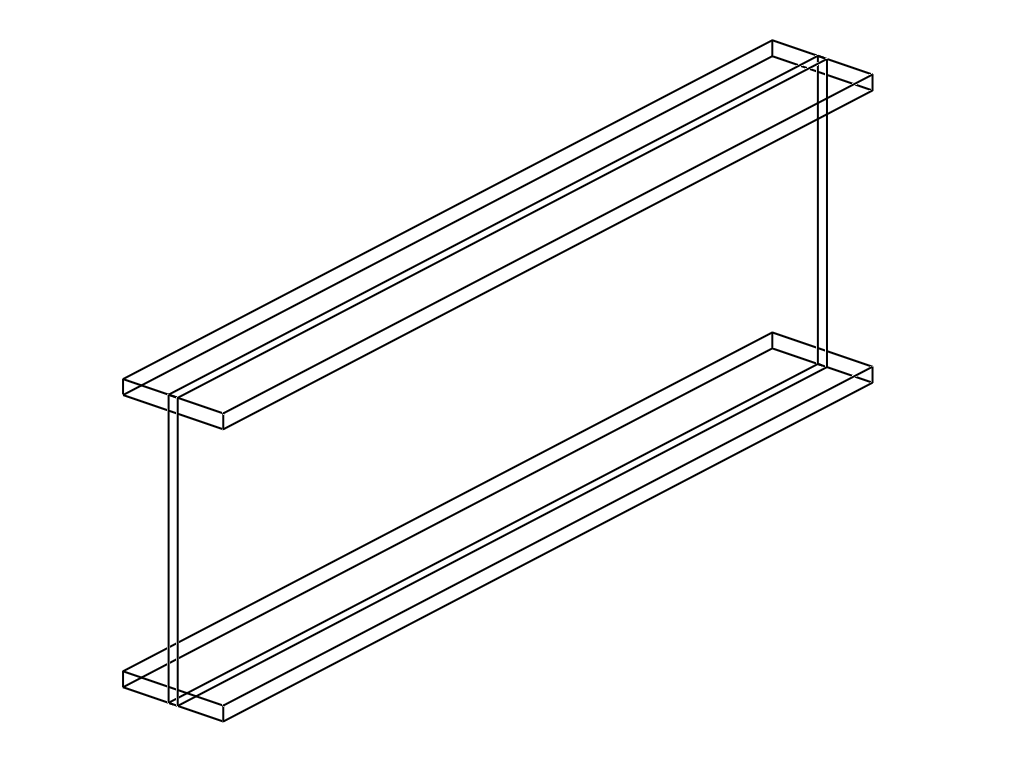
\includegraphics[height=2.0in]{FIGURES/ht3d_beam_heating_1_wire_2}
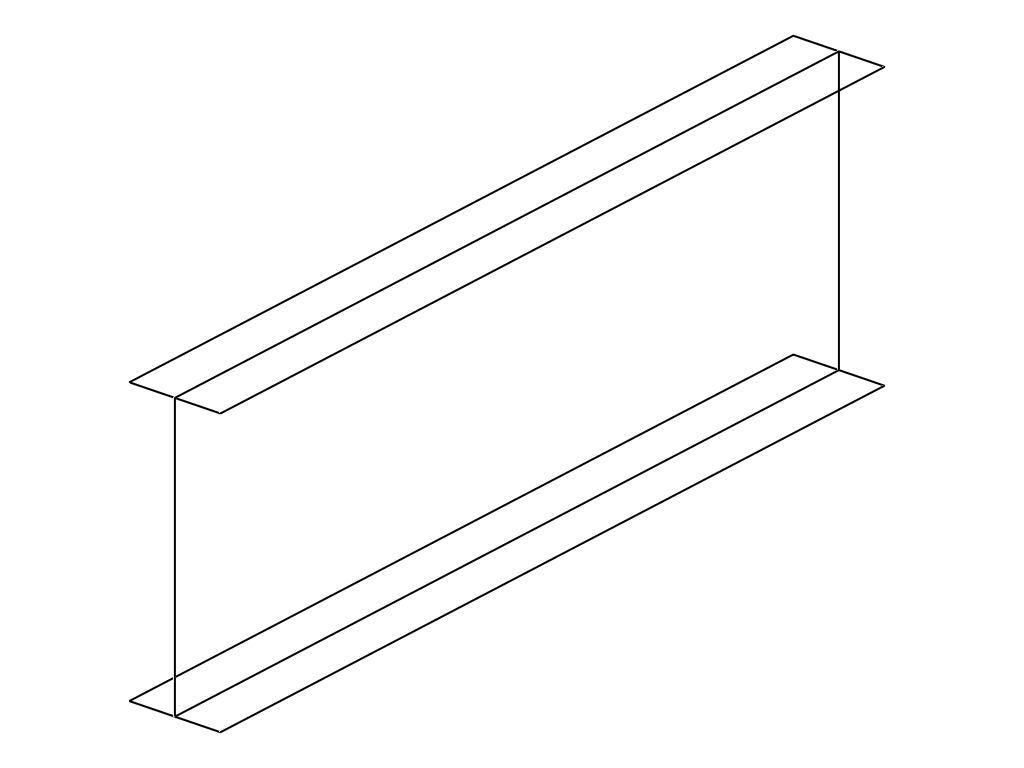
\includegraphics[height=2.0in]{FIGURES/ht3d_beam_heating_1_wire_1}
\caption[Schematic diagram of an I-beam]{(Left) Cross section of an I-beam. (Center) 3-D representation of the beam. (Right) FDS approximated thin obstructions.}
\label{fig:ht3d_beaming_heating}
\end{figure}


\subsubsection{Example: Coated Structural Steel}
\label{info:normal_direction_only}

An insulated steel beam can be modeled as a hybrid of 1-D and 3-D objects. The heat conducted through the insulation varies mainly in the direction normal to the surface, while the heat conducted along the steel beam varies mainly in the lateral direction. The following lines provide an example where a steel plate is coated with insulation. The steel plate is entered as a relatively thin obstruction, and the insulation is entered as a slightly thicker obstruction with a {\ct SURF} line that indicates that heat is to be conducted in the {\ct NORMAL\_DIRECTION\_ONLY} even though it is declared to be {\ct HT3D}. This latter parameter ensures that the thin steel obstruction and the insulation obstruction are included in the calculation of solid overlap volumes. Note that all dimensions are exact to ensure that the overlap volumes are computed properly.
\begin{lstlisting}
&OBST XB=0.12,1.88,0.51,0.53,0.21,0.79, SURF_ID='STEEL SLAB' /
&OBST XB=0.12,1.88,0.50,0.54,0.21,0.79, SURF_ID='WEB INSULATION' /
&SURF ID='STEEL SLAB', MATL_ID='STEEL', HT3D=T, COLOR='BLACK',
      CELL_SIZE=0.1, HEAT_TRANSFER_COEFFICIENT=20 /
&SURF ID='WEB INSULATION', MATL_ID='STUFF','STEEL','STUFF', COLOR='BEIGE',
      THICKNESS=0.010,0.020,0.010, HT3D=T, NORMAL_DIRECTION_ONLY=T /
\end{lstlisting}





\chapter{Fire and Pyrolysis}

FDS has several approaches for describing the pyrolysis of solids and liquids. The approach to take depends largely on the availability of material properties and the appropriateness of the underlying pyrolysis model. Note that all pyrolysis models in FDS require that you explicitly define the gas phase reaction. See Chapter~\ref{chap:combustion} for details. It should also be noted that the user has to use only one pyrolysis model at a time.

\section{Specified Heat Release Rate}
\label{multiple_reac_hrrpua}
\label{info:gas_burner}

Solids and liquid fuels can be modeled by specifying their relevant properties via the {\ct MATL} namelist group. However, if you simply want to specify a fire of a given heat release rate (HRR), you need not specify any material properties. A specified fire is basically modeled as the ejection of gaseous fuel from a solid surface or vent. This is essentially a burner, with a specified Heat Release Rate Per Unit Area, {\ct HRRPUA}, in units of kW/m$^2$. For example
\begin{lstlisting}
&SURF ID='FIRE', HRRPUA=500. /
\end{lstlisting}
applies 500~kW/m$^2$ to any surface with the attribute {\ct SURF\_ID='FIRE'}. See the discussion of time-dependent quantities in Chapter~\ref{info:RAMP} to learn how to ramp the heat release rate up and down.

An alternative to {\ct HRRPUA} with the exact same functionality is {\ct MLRPUA}, except this parameter
specifies the Mass Loss Rate of fuel gas Per Unit Area in \si{kg/(m$^2$.s)}. Do not specify both
{\ct HRRPUA} and {\ct MLRPUA} on the same {\ct SURF} line.

If either {\ct HRRPUA} or {\ct MLRPUA} are specified, but no {\ct SPEC\_ID} is given, then FDS will use the {\ct FUEL} for the first {\ct REAC} input. If a single {\ct SPEC\_ID} is given, then FDS will use that as the fuel. If multiple {\ct SPEC\_ID} along with {\ct MASS\_FRACTION} are given, then FDS will assume that the {\ct HRRPUA} or {\ct MLRPUA} refers to only species corresponding to {\ct FUEL} inputs on a {\ct REAC} line. For {\ct MLRPUA}, FDS will just multiply the {\ct MLRPUA} by the {\ct MASS\_FRACTION} of the fuel species to obtain the fuel species mass flux. If there are any non-fuel species, then the mass flux of those species will be set tp preserve their specified {\ct MASS\_FRACTION}. For {\ct HRRPUA}, FDS will compute the average heat of combustion for all the fuel species. This average heat of combustion is used to define the mass flux of fuel, i.e., the effective {\ct MLRPUA}. Non-fuel species are then treated as with {\ct MLRPUA}.

In the example below, six fuel species are used for four different surfaces with {\ct HRRPUA}. Four of the fuel species are predefined with no {\ct HEAT\_OF\_COMBUSTION} on their associated {\ct REAC} inputs; their heats of combustion can be determined using their heats of formation. One species has a {\ct HEAT\_OF\_COMBUSTION} on its {\ct REAC} input. The sixth fuel species is user defined and used in a {\ct REAC} with no {\ct HEAT\_OF\_COMBUSTION}. Its heat of combustion can be determined using {\ct EPUMO2}. surface {\ct S1} has {\ct HRRPUA} but no {\ct SPEC\_ID}; therefore, it will use the {\ct FUEL} species for the first {\ct REAC} input ({\ct METHANE}) for the fuel. The fuel mass flux for {\ct S1} will be given by the {\ct HRRPUA} divided by the {\ct METHANE} heat of combustion. Surface {\ct S2} specifies that the fuel species is {\ct MYFUEL}. Surface {\ct S3} will have a total mass flux computed using the {\ct MASS\_FLUX} weighted average of the heats of combustion for {\ct PROPANE} and {\ct ETHANE}. Surface {\ct S4} will use species {\ct MYFUEL2} whose heat of combustion will be the weighted average of the {\ct TOLUENE} and {\ct HYDROGEN} heats of combustion using the {\ct SPEC} input's {\ct MASS\_FRACTION}. Results are shown in Fig.~\ref{fig:mulitple_reac_hrrpua}.

\begin{lstlisting}
&SPEC ID='TOLUENE',LUMPED_COMPONENT_ONLY=T/
&SPEC ID='HYDROGEN',LUMPED_COMPONENT_ONLY=T/
&SPEC FUEL='MYFUEL',C=1,H=1,O=1/
&SPEC ID='MYFUEL2',SPEC_ID='TOLUENE','HYDROGEN',MASS_FRACTION=0.5,0.5/

&REAC FUEL='METHANE'/
&REAC FUEL='PROPANE'/
&REAC FUEL='ETHANE',HEAT_OF_COMBUSTION=40000/
&REAC FUEL='MYFUEL2'/

&SURF ID='S1',COLOR='RED',HRRPUA=1000/
&SURF ID='S2',COLOR='ORANGE',HRRPUA=1000,SPEC_ID='MYFUEL'/
&SURF ID='S3',COLOR='YELLOW',HRRPUA=1000,SPEC_ID='PROPANE','ETHANE',
      MASS_FRACTION=0.2,0.8/
&SURF ID='S4',COLOR='GREEN',HRRPUA=1000,SPEC_ID='MYFUEL2'/
\end{lstlisting}

If the second surface was specified as:

\begin{lstlisting}
&SURF ID='S2',COLOR='ORANGE',HRRPUA=1000,SPEC_ID='MYFUEL','NITROGEN',
      MASS_FRACTION=0.25,0.75/
\end{lstlisting}

then the fuel mass flux would be the same as before, but now it would be diluted with three times the mass flux of {\ct NITROGEN}.

\begin{figure}[ht]
\centering
\includegraphics[width=3.2in]{SCRIPT_FIGURES/multiple_reac_hrrpua}
\caption[Demonstration of specifying HRRPUA with multiple reactions.]{Demonstration of specifying HRRPUA with multiple reactions.}
\label{fig:mulitple_reac_hrrpua}
\end{figure}

\subsection{A Radially-Spreading Fire}
\label{info:spread}

Sometimes it is desired that a fire spread radially at some specified rate. Rather than trying to obtain material properties to directly model the ignition and spread of the fire, you can specify the fire spread rate directly. First, you need to add a {\ct SURF} line with a specified heat release rate, {\ct HRRPUA}, and an optional time history parameter, {\ct RAMP\_Q} or {\ct TAU\_Q} (see Section \ref{info:RAMP_Time}). Then, you must specify {\ct XYZ} and {\ct SPREAD\_RATE} on either a {\ct VENT} or the same {\ct SURF} line. The fire is directed to start at the point {\ct XYZ} (if unspecified, default is the center point of the {\ct VENT}) and spread radially at a rate of {\ct SPREAD\_RATE} (m/s). The optional ramp-up of the HRR begins at the time when the fire arrives at a given point. For example, the lines
\begin{lstlisting}
&SURF ID='FIRE', HRRPUA=500.0, RAMP_Q='fireramp' /
&RAMP ID='fireramp', T= 0.0, F=0.0 /
&RAMP ID='fireramp', T= 1.0, F=1.0 /
&RAMP ID='fireramp', T=30.0, F=1.0 /
&RAMP ID='fireramp', T=31.0, F=0.0 /
&VENT XB=0.0,5.0,1.5,9.5,0.0,0.0, SURF_ID='FIRE', XYZ=1.5,4.0,0.0, SPREAD_RATE=0.03 /
\end{lstlisting}
create a rectangular area via the {\ct VENT} line on which the fire starts at the point (1.5,4.0,0.0) and spreads outwards at a rate of 0.03~m/s. Each surface cell burns for 30~s as the fire spreads outward, creating a widening ring of fire. Note that the {\ct RAMP\_Q} is used to turn the burning on and off to simulate the consumption of fuel as the fire spreads radially. It should not be used to mimic a $t$-squared fire growth rate -- the whole point of the exercise is to mimic this curve in a more natural way. Eventually, the fire goes out as the ring grows past the boundary of the rectangle. Some trial and error is probably required to find the {\ct SPREAD\_RATE} that leads to a desired time history of the heat release rate.

If you desire that the fire spread over an area that is not confined to a flat plane, specify {\ct XYZ} and {\ct SPREAD\_RATE} on the {\ct SURF} line directly and then apply that {\ct SURF} line to the obstructions or particles over which you want the fire to spread. This technique can be useful for simulating the spread of fire through a cluttered space when the detailed properties of the materials are unknown, or when the uncertainties associated with modeling the pyrolysis of the solid fuels directly are too great.


If the starting time of the simulation, {\ct T\_BEGIN}, is not zero, be aware that the default start time of the radially spreading fire is {\ct T\_BEGIN}, not zero. This is also true of {\ct TAU\_Q}, but it is not true of {\ct RAMP\_Q}. Because this might be confusing, if you start the calculation at a time other than zero, do a quick test to ensure that the ramps or fire spread behave as expected.


\subsection{Compensating for the unresolved surface area}
\label{info:area_mult}

If the obstruction or vent with the pyrolysis model represents an object that has more complex shape than a rectangular box, or if the mesh resolution does not allow resolving the real surface area, you can add parameter {\ct AREA\_MULTIPLIER} on the {\ct SURF} line to manually adjust the burning rate with a constant factor. Default value is 1.0. This factor will also affect the rate of heat transfer between the object and gas phase.

\subsection{Thermally-Thick Solids that Burn at a Specified Rate}
\label{info:specified_burning}

Real objects, like furnishings, office equipment, and so on, are often difficult to describe via the {\ct SURF} and {\ct MATL} parameters. Sometimes the only information about a given object is its bulk thermal properties, its ``ignition'' temperature, and its subsequent burning rate as a function of time from ignition. For this situation, add lines similar to the following:
\begin{lstlisting}
&MATL ID                   = 'stuff'
      CONDUCTIVITY         = 0.1
      SPECIFIC_HEAT        = 1.0
      DENSITY              = 900.0 /

&SURF ID                   = 'my surface'
      COLOR                = 'GREEN'
      MATL_ID              = 'stuff'
      HRRPUA               = 1000.
      IGNITION_TEMPERATURE = 500.
      RAMP_Q               = 'fire_ramp'
      THICKNESS            = 0.01 /

&RAMP ID='fire_ramp', T=  0.0, F=0.0 /
&RAMP ID='fire_ramp', T= 10.0, F=1.0 /
&RAMP ID='fire_ramp', T=310.0, F=1.0 /
&RAMP ID='fire_ramp', T=320.0, F=0.0 /
\end{lstlisting}
An object with surface properties defined by {\ct 'my surface'} shall burn at a rate of 1000~kW/m$^2$ after a linear ramp-up of 10 s following its ``ignition'' when its surface temperature reaches 500~$^\circ$C. Burning shall continue for 5~min, and then ramp-down in 10~s. Note that the time {\ct T} in the {\ct RAMP} means time from ignition, not the time from the beginning of the simulation. Note also that now the ``ignition temperature'' is a surface property, not material property.

After the surface has ignited, the heat transfer into the solid is still calculated, but there is no coupling between the burning rate and the surface temperature. As a result, the surface temperature may increase too much. To account for the energy loss due to the vaporization of the solid fuel, {\ct HEAT\_OF\_VAPORIZATION} can be specified for the surface. For example, when using the lines below, the total heat flux at the material surface is reduced by a factor 1000~kJ/kg times the instantaneous burning rate.
\begin{lstlisting}
&SURF ID                   = 'my surface'
      COLOR                = 'GREEN'
      MATL_ID              = 'stuff'
      HRRPUA               = 1000.
      IGNITION_TEMPERATURE = 500.
      HEAT_OF_VAPORIZATION = 1000.
      RAMP_Q               = 'fire_ramp'
      THICKNESS            = 0.01 /
\end{lstlisting}
Finally, if you desire that the burning stop if the surface temperature drops below a specified value, set {\ct EXTINCTION\_TEMPERATURE} on the {\ct SURF} line. This value should be less than or equal to the \linebreak[4]{\ct IGNITION\_TEMPERATURE}.

The parameters {\ct HRRPUA}, {\ct IGNITION\_TEMPERATURE}, {\ct EXTINCTION\_TEMPERATURE}, and \linebreak[4]{\ct HEAT\_OF\_VAPORIZATION} are all telling FDS that you want to control the burning rate yourself, but you still want to simulate the heating up and ``ignition'' of the fuel. When these parameters appear on the {\ct SURF} line, they are acting in concert. If {\ct HRRPUA} appears alone, the surface will begin burning at the start of the simulation, like a piloted burner. The addition of an {\ct IGNITION\_TEMPERATURE} delays burning until your specified temperature is reached. The addition of {\ct HEAT\_OF\_VAPORIZATION} tells FDS to account for the energy used to vaporize the fuel. For any of these options, if a {\ct MATL} line is invoked by a {\ct SURF} line containing a specified {\ct HRRPUA}, then that {\ct MATL} ought to have only thermal properties. The {\ct MATL} line should have no reaction parameters, product yields, and so on, like those described in the previous sections. By specifying {\ct HRRPUA}, you are controlling the burning rate rather than letting the material pyrolyze based on the conditions of the surrounding environment. Also note that this simple model assumes that the solid acts like a typical {\em thermoplastic} material, i.e. it pyrolyzes near the surface leaving relatively little char.

\subsection{Scaling the Burning Rate by the Heat Flux}
\label{info:scaled_burning}

FDS has a simple model to extrapolate burning rate data collected from a cone calorimeter or similar device to the heat feedback occurring during an FDS simulation. This model is invoked by specifying a {\ct REFERENCE\_HEAT\_FLUX} along with {\ct HRRPUA}, {\ct IGNITION\_TEMPERATURE}, and {\ct RAMP\_Q} where \linebreak[4]{\ct REFERENCE\_HEAT\_FLUX} is the heat flux the test was conducted at and {\ct HRRPUA} and {\ct RAMP\_Q} define the burning rate where the test data is shifted so 0 s is the time the sample started burning in the test. When a wall cell reaches the {\ct IGNITION\_TEMPERATURE}, this model starts marching along the test data curve using a scaled time step where the scaled time step is the FDS time step adjusted by the ratio of {\ct REFERENCE\_HEAT\_FLUX} to the summation of the FDS incident radiative heat flux and net convective heat flux. At the scaled time, the ramp output is scaled by the ratio of the FDS incident flux to the {\ct REFERENCE\_HEAT\_FLUX}. Because the instantaneous heat flux at the surface varies significantly from time step to time step, the incident heat flux is time-averaged in this model. The default time-averaging window is 10 seconds, but this can be changed by the user by setting {\ct REFERENCE\_HEAT\_FLUX\_TIME\_INTERVAL} on the {\ct SURF} line. The time-averaged heat flux used in the scaling approach can be output as the boundary quantity {\ct REFERENCE\_HEAT\_FLUX}. The scaling-based pyrolysis model was developed on heat fluxes ranging from 25~kW/m$^2$ to 75~kW/m$^2$; however, by default the model does not limit the range of heat fluxes which are used in the scaling. This range can be modified by setting the surface quantities {\ct MINIMUM\_SCALING\_HEAT\_FLUX} and {\ct MAXIMUM\_SCALING\_HEAT\_FLUX}. An example where this may be desirable is in simulating fires with small ignition sources where the grid is not fine enough to resolve the flux from the initiating fuel.

An example demonstrating the scaling behavior is given below with results shown in Fig.~\ref{fig:cone_demo}. In this example a material with cone test data at 50 kW/m$^2$ is exposed to fluxes of 25, 50, and 75 kW/m$^2$. It can be seen that at 25 kW/m$^2$ the test data is stretched out in time by a factor of 2 with a reduction in burning rate of a factor of 2. Similarly at 75 kW/m$^2$, the curve is collapsed by 50~\% with the burning rate increased by 50~\%.

\begin{lstlisting}
&MATL ID='SAMPLE', CONDUCTIVITY=100, DENSITY=1000, SPECIFIC_HEAT=1, EMISSIVITY=1/

&SURF ID='SAMPLE25', IGNITION_TEMPERATURE=0, EXTERNAL_FLUX=25,
      HEAT_TRANSFER_COEFFICIENT=0, HRRPUA=1, RAMP_Q='CONE',
      REFERENCE_HEAT_FLUX=50,MATL_ID='SAMPLE',THICKNESS=0.01 /
&SURF ID='SAMPLE50', IGNITION_TEMPERATURE=0, EXTERNAL_FLUX=50,
      HEAT_TRANSFER_COEFFICIENT=0, HRRPUA=1, RAMP_Q='CONE',
      REFERENCE_HEAT_FLUX=50, MATL_ID='SAMPLE', THICKNESS=0.01 /
&SURF ID='SAMPLE75', IGNITION_TEMPERATURE=0, EXTERNAL_FLUX=75,
      HEAT_TRANSFER_COEFFICIENT=0, HRRPUA=1, RAMP_Q='CONE',
      REFERENCE_HEAT_FLUX=50, MATL_ID='SAMPLE', THICKNESS=0.01 /

&VENT XB=0.1,0.3,0.0,0.1,0.0,0.0, SURF_ID='SAMPLE25' /
&VENT XB=0.6,0.7,0.0,0.1,0.0,0.0, SURF_ID='SAMPLE50' /
&VENT XB=1.1,1.2,0.0,0.1,0.0,0.0, SURF_ID='SAMPLE75' /

&RAMP ID='CONE', T=0, F=0/
&RAMP ID='CONE', T=1, F=2.03437906875814 /
&RAMP ID='CONE', T=2, F=2.12156674313349 /
...
&RAMP ID='CONE', T=509, F=43.0125860251721 /
&RAMP ID='CONE', T=510, F=0/
\end{lstlisting}

\begin{figure}[ht]
\centering
\includegraphics[width=3.2in]{SCRIPT_FIGURES/cone_demo}
\caption[Demonstration of extrapolating cone test data to other heat fluxes.]{Demonstration of extrapolating cone test data to other heat fluxes.}
\label{fig:cone_demo}
\end{figure}


\newpage

\section{Complex Pyrolysis Models}
\label{info:solid_pyrolysis}

This section describes the parameters that describe the reactions that occur within solid
materials when they are burning. It is strongly recommended before reading this section that you read some background material on
solid phase pyrolysis, for example ``Thermal Decomposition of Polymeric Materials,'' by Witkowski, Stec, and Hull, or
``Flaming Ignition of Solid Fuels,'' by Torero, both of which are in the 5th edition of the
{\em SFPE Handbook of Fire Protection Engineering}.

\subsection{Reaction Mechanism}

A solid surface in FDS may consist of multiple layers with multiple material components per layer. The material components are described via {\ct MATL} lines and are specified on the {\ct SURF} line that describes the structure of the solid.  Each {\ct MATL} can undergo several reactions that may occur at different temperatures. It may not undergo any -- it may just heat up. However, if it is to change form via one or more reactions, designate the number of reactions with the integer {\ct N\_REACTIONS}. It is very important that you designate {\ct N\_REACTIONS} or else FDS will ignore all parameters associated with reactions. Note that experimental evidence of multiple reactions does not imply that a single material is undergoing multiple reactions, but rather that multiple material components are undergoing individual reactions at distinct temperatures.  Currently, the maximum number of reactions for each material is 10 and the chain of consecutive reactions may contain up to 20 steps.

For a given material, the $j$th reaction can produce other solid materials whose names are designated with \linebreak[4] {\ct MATL\_ID(i,j)}, gas species whose names are designated with {\ct SPEC\_ID(i,j)}, and particles whose particle classes are are designated with {\ct PART\_ID(i,j)}. Note that the index, $i$, runs from 1 to the number of materials, gaseous species, or particle classes. This index does {\em not} correspond to the order in which the {\ct MATL} or {\ct SPEC} lines are listed in the input file. For a given reaction, the relative amounts of solid, gaseous, or particle products are input to FDS via the {\em yields}: {\ct NU\_MATL(i,j)}, {\ct NU\_SPEC(i,j)}, and {\ct NU\_PART(i,j)}, respectively. The yields are all zero by default. If {\ct NU\_MATL(i,j)} is non-zero, then you {\em must} indicate what the solid residue is via {\ct MATL\_ID(i,j)}, the {\ct ID} of another {\ct MATL} that is also listed in the input file.  If {\ct NU\_SPEC(i,j)} is non-zero, then you {\em must} indicate what the gas species is via {\ct SPEC\_ID(i,j)}, the {\ct ID} of another {\ct SPEC} that is also listed in the input file. If {\ct NU\_PART(i,j)} is non-zero, then you {\em must} indicate what the particle class is via {\ct PART\_ID(i,j)}, the {\ct ID} of another {\ct PART} that is also listed in the input file. If particles are specified, the insertion rate and number of particles is controlled via the particle inputs on the {\ct SURF} containing the material. Ideally, the sum of the yields should add to 1, meaning that the mass of the reactant is conserved. However, there are times when it is convenient to have the yields sum to something less than one. For example, the spalling or ablation of concrete can be described as a ``reaction'' that consumes energy but does not produce any ``product'' because the concrete is assumed to have either fallen off the surface in chunks or pulverized powder. The concrete's mass is not conserved {\em in the model} because it has essentially disappeared from that particular surface. Producing more mass (yields more than 1) will result in an error message.

For consistency, the {\ct HEAT\_OF\_COMBUSTION(i,j)} can also be specified for each species, $i$, in each reaction, $j$. These values are used only if the corresponding heats of combustion for the gaseous species are greater than zero.  Note that {\ct HEAT\_OF\_COMBUSTION(i,j)} discussed here is not necessarily the same as the {\ct HEAT\_OF\_COMBUSTION} of the surrogate {\ct FUEL} used for gas phase combustion (e.g., {\ct 'PROPANE'}).  When the heats of combustion differ, the mass flux of the surrogate {\ct FUEL} in the gas phase is adjusted so that the correct heat release rate is attained.  This is further discussed in the next section.

In the example below, the pyrolysis of wood is included within a simulation that uses a finite-rate reaction instead of the default mixing-controlled model. Notice in this case that all of the gas species (except for the background nitrogen) are explicitly defined, and as a result, FDS needs to be told explicitly what gaseous species are produced by the solid phase reactions. In this case, 82~\% of the mass of wood is converted to gaseous {\ct 'PYROLYZATE'} and 18~\% is converted to solid {\ct 'CHAR'}.
\begin{lstlisting}
&SPEC ID = 'PYROLYZATE', MW=53.6 /
&SPEC ID = 'OXYGEN', MASS_FRACTION_0 = 0.23 /
&SPEC ID = 'WATER VAPOR' /
&SPEC ID = 'CARBON DIOXIDE' /

&MATL ID                    = 'WOOD'
      EMISSIVITY            = 0.9
      CONDUCTIVITY          = 0.2
      SPECIFIC_HEAT         = 1.3
      DENSITY               = 570.
      N_REACTIONS           = 1
      A(1)                  = 1.89E10
      E(1)                  = 1.51E5
      N_S(1)                = 1.0
      MATL_ID(1,1)          = 'CHAR'
      NU_MATL(1,1)          = 0.18
      SPEC_ID(1:4,1)        = 'OXYGEN','WATER VAPOR','CARBON DIOXIDE','PYROLYZATE'
      NU_SPEC(1:4,1)        = 0,0,0,0.82
      HEAT_OF_REACTION(1)   = 430.
      HEAT_OF_COMBUSTION(4,1)= 14500. /
\end{lstlisting}
Note that the indices associated with the parameters are not needed {\em in this case}, but they are shown to emphasize that, in general, there can be multiple reactions with corresponding kinetic parameters and products.

\subsection{Reaction Rates}
\label{sec:reaction_rates}

The mass per unit volume of material component $i$, $\rho_{{\rm s},i}(x,t)$, is a function of the depth into the solid, $x$, and time, $t$. It evolves in time according to the following equation:
\be
  \frac{\partial \rho_{{\rm s},i}}{\partial t} = - \sum_{j=1}^{N_{{\rm r},i}} r_{ij} + \sum_{i'=1}^{N_{\rm m}} \sum_{j=1}^{N_{{\rm r},i'}} \nu_{{\rm s},i'j} \; r_{i'j} \quad (i' \neq i)
\label{rr_tot}
\ee
where
\be
  r_{ij} = A_{ij} \; \rho_{{\rm s},i}^{n_{{\rm s},ij}} \;  T_{\rm s}^{n_{{\rm t},ij}} \; \exp \left(-\frac{E_{ij}}{R \, T_{\rm s}} \right) X_{\rm O_2}^{n_{{\rm O_2},ij}}
  \label{rr}
\ee
The term, $r_{ij}$, defines the rate of reaction at the temperature, $T_{\rm s}$, of the $i$th material undergoing its $j$th reaction. The second term on the right of the equation (\ref{rr_tot}) represents the contributions of other materials producing the $i$th material as a residue with a yield of $\nu_{{\rm s},i'j}$. This term is denoted by {\ct NU\_MATL(:,j)} on the $i'$-th {\ct MATL} line. $\rho_{{\rm s},i}$ is the density of the $i$th material component of the layer, defined as the mass of the $i$th material component divided by the volume of the layer. Thus, $\rho_{{\rm s},i}$ is a quantity that increases if the $i$th material component is produced as a residue of some other reaction, or decreases if the $i$th component decomposes. $n_{{\rm s},ij}$ is the reaction order and prescribed under the name {\ct N\_S(j)}, and is 1 by default. If the value of $n_{\rm s}$ is not known, it is a good starting point to assume it is 1.  $n_{{\rm t},j}$ is prescribed under the name {\ct N\_T(j)}. By default, $n_{{\rm t},j}$ is zero.

The pre-exponential factor\footnote{For versions of FDS up to and including 6.7.7, the form of the reaction rate expression was slightly different than the one currently used. In these older versions, the density term on the right hand side of Eq.~(\ref{rr}) was divided by the initial density of the layer. For first-order reactions ($n_{{\rm s},ij}=1$), this older form is equivalent to the current form. However, for reactions that are not first-order ($n_{{\rm s},ij}\neq 1$), the new value of $A_{ij}=A_{ij}^{\rm old}/\rho_{\rm s}(0)^{n_{{\rm s},ij}-1}$, where $\rho_{\rm s}(0)$ is the initial density of the layer.}, $A_{ij}$, is prescribed under the name {\ct A(j)} on the {\ct MATL} line of the $i$th material, with units of s$^{-1}$. $E_{ij}$, the activation energy, is prescribed via {\ct E(j)} in units of J/mol. Remember that 1~kcal is 4.184~kJ, and be careful with factors of 1000. For a given reaction, specify both $A$ and $E$, or neither. Do not specify only one of these two parameters. Typically, these parameters only have meaning when both are derived from a common set of experiments, like TGA (thermogravimetric analysis).

The fourth term of the reaction rate equation (\ref{rr}) can be used to simulate oxidation reactions. If the heterogeneous reaction order $n_{{\rm O_2},ij}$ is greater than zero, the reaction rate is affected by the local oxygen volume fraction, $X_{\rm O_2}$. It is calculated from the gas phase (first grid cell) oxygen volume fraction $X_{\rm O_2,g}$ by assuming simultaneous diffusion and consumption so that the concentration profile is in equilibrium, and the concentration at depth $x$ is given by
\be
X_{\rm O_2}(x) = X_{\rm O_2,g}\exp(-x/L_{\rm g})
\ee
where $L_{\rm g}$ is the gas diffusion length scale. $n_{{\rm O_2},ij}$ is prescribed under the name {\ct N\_O2(j)} on the {\ct MATL} line of the $i$th material. It is zero by default. $L_{\rm g}$ is prescribed under the name {\ct GAS\_DIFFUSION\_DEPTH(j)}, and it is 0.001 m by default.

You can specity {\ct MAX\_REACTION\_RATE(j)} (1/s) to limit the reaction rate, $r_{ij}$, below a specified value.


\subsubsection{Estimating Kinetic Parameters}
\label{info:kinetic_parameters}

The kinetic constants, $A$ and $E$, are typically not available for most real materials.  However, there is a way to model material decomposition using a simplified reaction scheme. The key assumption is that each material component undergoes only one reaction. If, for example, the composite material undergoes three distinct reactions, it must be represented by three material components, each of which undergoes one reaction. If there is an additional residue left over, then a fourth material component is needed. Any or all of the material components can leave behind a residue.

In lieu of specifying $A$ and $E$, there are several parameters that can be used by FDS to derive effective values, the most important of which is the  {\ct REFERENCE\_TEMPERATURE} ($^\circ$C). To understand this parameter, consider the plot shown in Fig.~\ref{pyrolysis}. These curves represent the results of a hypothetical TGA experiment in which a single component material undergoes a single reaction that converts the solid into a gas. The Normalized Mass (blue curve, $Y_{\rm s}$) decreases as the sample is slowly heated, in this case at a rate of 5~K/min. The Normalized Mass Loss Rate (red curve) is the rate of change of the normalized mass as a function of time ($-\d Y_{\rm s}/\d t$). Where this curve peaks is referred to in FDS as the {\ct REFERENCE\_TEMPERATURE}, which is not necessarily equivalent to an ignition temperature, nor is it necessarily the surface temperature of the burning solid. Rather, it is simply the temperature at which the mass fraction of the material decreases at its maximum rate within the context of a TGA or similar experimental apparatus.

The kinetic constants for component $i$ of a multi-component solid are given by\footnote{These formulas have been derived from an analysis that considers a first-order reaction. When using this method, do not specify a non-unity value for the reaction order {\ct N\_S} on the {\ct MATL} line.}:
\be
   E_{i,1} = \frac{ {\rm e} \, r_{{\rm p},i} }{ Y_{{\rm s},i}(0) } \, \frac{R \, T_{{\rm p},i}^2}{\dot{T}} \quad ; \quad
   A_{i,1} = \frac{ {\rm e} \, r_{{\rm p},i} }{ Y_{{\rm s},i}(0) } \, {\rm e}^{E/R \, T_{{\rm p},i}} \label{AandE}
\ee
where $T_{{\rm p},i}$ and $r_{{\rm p},i}/Y_{{\rm s},i}(0)$ are the reference temperature and rate, respectively. The {\ct REFERENCE\_RATE} is the normalized mass loss rate, in units of s$^{-1}$, at the given {\ct REFERENCE\_TEMPERATURE} divided by the mass fraction, $Y_{{\rm s},i}(0)$, of the material component in the original sample undergoing the reaction. For a single component, single reaction material, $Y_{{\rm s},1}(0)=1$. The {\ct HEATING\_RATE} ($\dot{T}$) is the rate at which the temperature of the TGA (or equivalent) test apparatus was increased. It is input into FDS in units of K/min (in the formula, it is expressed in K/s). Its default value is 5~K/min. In Fig.~\ref{pyrolysis}, the area under the red curve (Normalized Mass Loss Rate) is equal to the heating rate (in units of K/s).

\begin{figure}[ht]
\noindent
\begin{minipage}{0.5\textwidth}
\includegraphics[width=3.2in]{SCRIPT_FIGURES/pyrolysis_1}
\end{minipage}
\hfill
\begin{minipage}{0.5\textwidth}
\begin{equation*}
   \frac{\d Y_{\rm s}}{\d t} = -A \, Y_{\rm s} \, \exp(-E/RT_{\rm s})   \quad \; \quad    Y_{\rm s}(0) =1
\end{equation*}
\begin{align*}
   T_{\rm p} &= 300 \; ^\circ\mathrm{C}  \\
   r_{\rm p} &= 0.002   \; \mathrm{s}^{-1}  \\
   \dot{T} &= 5 \; \mathrm{K/min} \\
   \nu_{\rm s} &= 0 \\
\end{align*}
\end{minipage}
\caption[Simple demonstration of the pyrolysis model]{The blue curve represents the normalized mass, $Y_{\rm s}=\rho_{\rm s}/\rho_{\rm s}(0)$, of a solid material undergoing heating at a rate of 5~K/min. The red curve represents the reaction rate, $-\d Y_{\rm s}/\d t$. The ordinary differential equation that describes the transformation is shown at right. Note that the parameters $T_{\rm p}$, $r_{\rm p}$, and $\nu_{\rm s}$ represent the ``reference'' temperature, reaction rate, and residue yield of the single reaction. From these parameters, values of $A$ and $E$ can be estimated using the formulae in (\ref{AandE}). The full set of parameters for this case are listed in {\ct pyrolysis\_1.fds}.}
\label{pyrolysis}
\end{figure}

There are many cases where it is only possible to estimate the {\ct REFERENCE\_TEMPERATURE} ($T_{\rm p}$) of a particular reaction because micro-scale calorimetry data is unavailable. In such cases, an additional parameter can be specified to help fine tune the shape of the reaction rate curve, assuming some sort of measurement or estimate has been made to indicate at what temperature, and over what temperature range, the reaction takes place. The {\ct PYROLYSIS\_RANGE} ($\Delta T$) is the approximate width (in degrees Celsius or Kelvin) of the normalized mass loss rate curve, assuming its shape to be roughly triangular. Its default value is 80~$^\circ$C. Using these input parameters, an estimate is made of the peak reaction rate, $r_{{\rm p},i}$, with which $E_{i,1}$, then $A_{i,1}$, are calculated.
\be
   \frac{r_{{\rm p},i}}{Y_{{\rm s},i}(0)} = \frac{2 \, \dot{T}} {\Delta T} \, (1-\nu_{{\rm s},i}) \label{r_p}
\ee
The parameter, $\nu_{{\rm s},i}$, is the yield of solid residue.

When in doubt about the values of these various parameters, just specify the {\ct REFERENCE\_TEMPERATURE}. Note that FDS will automatically calculate $A$ and $E$ using the above formulae. Do not specify $A$ and $E$ if you specify the \linebreak[3] {\ct REFERENCE\_TEMPERATURE}, and do not specify {\ct PYROLYSIS\_RANGE} if you specify {\ct REFERENCE\_RATE}. For the material decomposition shown in Fig.~\ref{pyrolysis}, the {\ct MATL} would have the form:
\begin{lstlisting}
&MATL ID                       = 'My Fuel'
      ...
      N_REACTIONS              = 1
      SPEC_ID(1,1)             = '...'
      NU_SPEC(1,1)             = 1.
      REFERENCE_TEMPERATURE(1) = 300.
      REFERENCE_RATE(1)        = 0.002
      HEATING_RATE(1)          = 5.
      HEAT_OF_COMBUSTION(1)    = ...
      HEAT_OF_REACTION(1)      = ... /
\end{lstlisting}
Note that the indices have been added to the reaction parameters to emphasize the fact that these parameters are stored in arrays of length equal to {\ct N\_REACTIONS}. If there is only one reaction, you need not include the {\ct (1)}, but it is a good habit to get into. Note also that if the default combustion model is used, you can denote that the reaction produces fuel gas using the appropriate {\ct SPEC\_ID}. Note also that the {\ct HEAT\_OF\_COMBUSTION} is the energy released per unit mass of fuel gas that mixes with oxygen and combusts.  This has nothing to do with the pyrolysis process, so why is it specified here? The answer is that when using the default combustion model in FDS there is only one {\em gas phase} reaction of fuel and oxygen, but there can be dozens of different materials and dozens of {\em solid phase} reactions. To ensure that the fuel vapors from different materials combust to produce the proper amount of energy, it is very important to specify a {\ct HEAT\_OF\_COMBUSTION} for each material. That way, the mass loss rate of fuel gases is automatically adjusted so that the effective mass loss rate multiplied by the single, global, gas phase heat of combustion produces the expected heat release rate. This adjustment uses the value of {\ct HOC\_COMPLETE}, see Sec.~\ref{info:hoc_complete}, on the {\ct REAC} line. If, for example, the {\ct HOC\_COMPLETE} specified on the {\ct REAC} line is twice that specified on the {\ct MATL} line, the mass of contained within wall cell will be decremented by that determined by the pyrolysis model, but the mass added to gas phase would be reduced by 50~\%. A different value of heat of combustion can be specified for each species, $i$, in each reaction, $j$, via the parameter {\ct HEAT\_OF\_COMBUSTION(i,j)}.

\subsubsection{Modeling Upholstered Furnishings}
\label{couch}

The example input file called {\ct Fires/couch.fds} demonstrates a simple way to model upholstered furniture. Modeling a couch requires a simplification of its structure and materials.  At the very least, we want the upholstery to be modeled as a layer of fabric covering polyurethane foam. We need the thermal properties of each, along with estimates of the ``reference'' temperatures as described above. The foam might be described as follows:
\begin{lstlisting}
&MATL ID                    = 'FOAM'
      SPECIFIC_HEAT         = 1.0
      CONDUCTIVITY          = 0.1
      DENSITY               = 40.0
      NU_SPEC               = 1.
      SPEC_ID               = 'POLYURETHANE'
      REFERENCE_TEMPERATURE = 280.
      HEAT_OF_REACTION      = 800. /
\end{lstlisting}
Note that these properties are completely made up.  Both the fabric and the foam decompose into fuel gases via single-step reactions. The fuel gases from each have different composition and heats of combustion. FDS automatically adjusts the mass loss rate of each so that the ``effective'' fuel gas is that which is specified on the {\ct REAC} line.  Figure~\ref{couch_fig} shows the fire after 1~min, 2~min, 3~min, and 10~min. Only the flame zone of the fire is shown; the smoke is hidden so that you can see the fire progressing along the couch. Also shown in the Fig.~\ref{couch_fig} is the heat release rate of the burning couch. The ``Expected HRR'' is a rough estimate of the peak HRR of a piece of furniture of this size.

\begin{figure}[!ht]
\begin{tabular*}{\textwidth}{l@{\extracolsep{\fill}}r}
\includegraphics[height=2.15in]{SCRIPT_FIGURES/couch_60} &
\includegraphics[height=2.15in]{SCRIPT_FIGURES/couch_120} \\
\includegraphics[height=2.15in]{SCRIPT_FIGURES/couch_180} &
\includegraphics[height=2.15in]{SCRIPT_FIGURES/couch_600} \\
\multicolumn{2}{c}{\includegraphics[height=2.15in]{SCRIPT_FIGURES/couch}}
\end{tabular*}
\caption[Results of the {\ct couch} test case]{Smokeview images of the {\ct couch} test case after 1, 2, 3, and 10 min, plus the heat release rate as a function of time.}
\label{couch_fig}
\end{figure}

\FloatBarrier

\subsection{Shrinking and Swelling materials}
\label{info:shrink_swell}

Many practical materials change in thickness during the thermal reactions. For example:
\begin{itemize}
\item Non-charring materials will shrink as material is removed from the condensed phase to the gas phase.
\item Porous materials like foams would shrink when the material melts and forms a non-porous layer.
\item Some charring materials swell, i.e., get thicker, when a porous char layer is formed.
\item Intumescent fire protection materials would swell significantly, creating an insulating layer.
\end{itemize}
In FDS, the layer thickness is updated according to the ratio of the instantaneous material density and the density of the material in its pure form, i.e.,
the {\ct DENSITY} on the {\ct MATL} line. In cases involving several material components, the amount of swelling and shrinking is determined by the maximum and sum of these ratios, respectively. In mathematical terms, this means that in each time step the size of each condensed phase cell is changed according to the ratio $\delta$
\be
\delta =
   \begin{cases}
   \max_i\left(\frac{\rho_{{\rm s},i}}{\rho_i}\right) & \text{if } \max_i \left(\frac{\rho_{{\rm s},i}}{\rho_i}\right)\geq 1 \\
   \sum_i\left(\frac{\rho_{{\rm s},i}}{\rho_i}\right) & \text{if } \max_i \left(\frac{\rho_{{\rm s},i}}{\rho_i}\right)<1
   \end{cases}
\ee
For example, if the original material with a {\ct DENSITY} of 500~kg/m$^3$ is completely converted into a residue with a {\ct DENSITY} of 1000~kg/m$^3$, the thickness of the material layer will be half of the original.

You can prevent shrinking by setting {\ct ALLOW\_SHRINKING} to {\ct F} on the {\ct MATL} line. You can prevent swelling by specifying
{\ct ALLOW\_SWELLING} to {\ct F} on the {\ct MATL} line.  By default, these flags are true. Shrinking/swelling does not take place if any of the materials with non-zero density has the corresponding flag set to false.



\subsection{Multiple Solid Phase Reactions}

The solid phase reaction represented by Fig.~\ref{pyrolysis} is fairly simple---a single, homogeneous material is heated and gasified completely. Figure~\ref{pyrolysis_2} depicts a more complicated case. Here, a solid material that contains 10~\% (by mass) water and 90~\% dry solid. The water evaporates in the neighborhood of 100~$^\circ$C and the dry solid then pyrolyzes in the neighborhood of 300~$^\circ$C, leaving 20~\% of its mass behind in the form of a solid residue. The full set of parameters for this case are listed in {\ct pyrolysis\_2.fds}.

\begin{figure}[ht]
\noindent
\begin{minipage}{0.5\textwidth}
\includegraphics[width=3.2in]{SCRIPT_FIGURES/pyrolysis_2}
\end{minipage}
\hfill
\begin{minipage}{0.5\textwidth}
\footnotesize
\begin{align*}
   \frac{\d Y_{\rm s,1}}{\d t} &= -A_{1,1} \, Y_{\rm s,1} \, \exp(-E_{1,1}/RT_{\rm s})                  & Y_{\rm s,1}(0) &=0.1 \\
   \frac{\d Y_{\rm s,2}}{\d t} &= -A_{2,1} \, Y_{\rm s,2} \, \exp(-E_{2,1}/RT_{\rm s})                  & Y_{\rm s,2}(0) &=0.9 \\
   \frac{\d Y_{\rm s,3}}{\d t} &= -\nu_{{\rm s},2,1} \frac{\d Y_{\rm s,2}}{\d t}                        & Y_{\rm s,3}(0) &=0.0
\end{align*}
\begin{align*}
   T_{{\rm p},1,1} &= 100+273 \; \mathrm{K}        & T_{{\rm p},2,1}   &= 300+273 \; \mathrm{K} \\
   r_{{\rm p},1,1} &= 0.0016 \; \mathrm{s}^{-1}           & r_{{\rm p},2,1}   &= 0.0012 \; \mathrm{s}^{-1} \\
   \nu_{{\rm s},1,1} &= 0                          & \nu_{{\rm s},2,1} &= 0.2 \\
   \dot{T} &= 5 \; \mathrm{K/min} & &
\end{align*}
\end{minipage} \normalsize
\caption[A more complicated demonstration of the pyrolysis model]{Normalized mass ($\sum Y_{{\rm s},i}$, blue curve) and mass loss rate ($\sum \d Y_{{\rm s},i}/\d t$, red curve) for a material that contains 10~\% water (by mass) that evaporates at a temperature of 100~$^\circ$C, and 90~\% solid material that pyrolyzes at 300~$^\circ$C, leaving a 20~\% (by mass) residue behind. Note that the numbered subscripts refer to the material component and the reaction, respectively. The system of ordinary differential equations that governs the transformation of the materials is shown at right.}
\label{pyrolysis_2}
\end{figure}

The plot in Fig.~\ref{pyrolysis_2} contains two sets of curves. The solid curves represent the solution of the set of equations computed using a Matlab ODE solver, and the underlying dashed curves are a ``fit'' of the Matlab solution using FDS. The {\ct MATL} line for the solid material contains the following three parameters that define its decomposition:
\begin{lstlisting}
&MATL ID                    = '...'
      ...
      REFERENCE_TEMPERATURE = 300.
      PYROLYSIS_RANGE       = 100.
      HEATING_RATE          = 5.   /
\end{lstlisting}
The {\ct REFERENCE\_TEMPERATURE} is the temperature in $^\circ$C where the mass loss rate is at its peak. The {\ct HEATING\_RATE} is the linear temperature rise ($^\circ$C/min) used in the TGA experiment, which is represented here by the Matlab solution. The {\ct PYROLYSIS\_RANGE} is the approximate ``width'' of the second red hump in Fig.~\ref{pyrolysis_2}, fit by inspection. That is, the value of 100~$^\circ$C was chosen by trial and error. This is typically how one would choose kinetic parameters in FDS to match a given TGA curve.




\subsection{The Heat of Reaction}

Equation~(\ref{rr}) describes the rate of the reaction as a function of temperature.  Most solid phase reactions require energy; that is, they are {\em endothermic}. The amount of energy consumed, per unit mass of reactant that is converted into reaction products, is specified by the {\ct HEAT\_OF\_REACTION(j)}. Technically, this is the enthalpy difference between the products and the reactant. A positive value indicates that the reaction is {\em endothermic}; that is, the reaction takes energy out of the system. Usually the {\ct HEAT\_OF\_REACTION} is accurately known only for simple phase change reactions like the vaporization of water. For other reactions, it must be determined empirically (e.g., by differential scanning calorimetry).



\subsection{Liquid Fuels}
\label{info:liquid_fuels}

For a liquid fuel, the thermal properties are similar to those of a solid material, with a few exceptions. The evaporation rate of the fuel is governed by the mass transfer number (see FDS Technical Reference Guide for details). The properties of a liquid fuel are given on the {\ct MATL} line:
\begin{lstlisting}
&REAC FUEL               = 'ETHANOL'
      CO_YIELD           = 0.001
      SOOT_YIELD         = 0.008 /

&MATL ID                     = 'ETHANOL LIQUID'
      EMISSIVITY             = 1.
      NU_SPEC                = 1.
      SPEC_ID                = 'ETHANOL'
      HEAT_OF_REACTION       = 837
      CONDUCTIVITY           = 0.17
      SPECIFIC_HEAT          = 2.44
      DENSITY                = 794
      ABSORPTION_COEFFICIENT = 1140
      BOILING_TEMPERATURE    = 78.5 /

&SURF ID        = 'ETHANOL POOL'
      COLOR     = 'YELLOW'
      MATL_ID   = 'ETHANOL LIQUID'
      THICKNESS = 0.1 /
\end{lstlisting}
The inclusion of {\ct BOILING\_TEMPERATURE} on the {\ct MATL} line tells FDS to use its liquid pyrolysis model. It also automatically sets {\ct N\_REACTIONS=1}, that is, the only ``reaction'' is the phase change from liquid to gaseous fuel. Thus, {\ct HEAT\_OF\_REACTION} in this case is the latent heat of vaporization. The thermal conductivity, density and specific heat are used to compute the loss of heat into the liquid via conduction using the same one-dimensional heat transfer equation that is used for solids. Obviously, the convection of the liquid is important, but is not considered in the model. The {\ct ABSORPTION\_COEFFICIENT} denotes the absorption in depth of thermal radiation into the liquid. Liquids do not just absorb radiation at the surface, but rather over a thin layer near the surface. Its effect on the burning rate can be significant.

In this example, {\ct 'ETHANOL'} is a {\em known} species; that is, it is listed in Appendix~\ref{info:predefined_species}. For this reason, you only need to specify its CO and soot yield. If it is not known, then you must furnish additional information. Sec.~\ref{user_defined_gas_species_props} contains details, but in brief, only the molecular weight of the gas species is of relevance for the liquid pool evaporation model. If the liquid has multiple components, like gasoline or kerosene, you can furnish an individual {\ct MATL} line for each component. For practical reasons, in such cases you might still want to assume only one gas phase fuel species; thus, each {\ct MATL} line would contain the same {\ct SPEC\_ID}. If this is the case, provide the liquid component molecular weights, {\ct MW}, with units of g/mol on the {\ct MATL} lines. These unique molecular weights are used when computing the evaporation rates of the individual liquid components.

\subsubsection{Evaporation of a Pure Liquid}
\label{methanol_evaporation}

An example of liquid evaporation is given by the sample case found in the {\ct Pyrolysis} folder called {\ct methanol\_evaporation.fds}. A 1~m by 1~m pan filled with methanol at $T_\infty=20$~$^\circ$C is exposed to a uniform heat flux, $\dot{q}''=20$~kW/m$^2$. The boiling temperature of methanol is $T_{\rm b}=64.65$~$^\circ$C, its specific heat, $c=2.48$~kJ/(kg$\cdot$K), and heat of vaporization, $h_{\rm v}=1099$~kJ/kg. The evaporation rate of a burning liquid in steady state is approximately
\be
   \dot{m}'' \approx \frac{\dot{q}''}{h_{\rm g}}  \quad ; \quad  h_{\rm g} = c (T_{\rm b}-T_\infty) + h_{\rm v}
\ee
In this example, the methanol evaporates in an oxygen-depleted atmosphere and no burning occurs. The left hand plot in Fig.~\ref{methanol_evaporation_plot} displays the computed evaporation rate, $\dot{m}''$, versus the ideal, $\dot{q}''/h_{\rm g}$. The former approaches the latter as all of the absorbed energy is used to evaporate the liquid. The right hand plot shows the computed liquid surface temperature versus the liquid boiling temperature.
\begin{figure}[!ht]
\includegraphics[width=3.2in]{SCRIPT_FIGURES/methanol_evaporation_mdot}
\includegraphics[width=3.2in]{SCRIPT_FIGURES/methanol_evaporation_temp}
\caption[Results of the {\ct methanol\_evaporation} test case]{(Left) Mass loss rate of the methanol versus its expected steady state value. (Right) Computed surface temperature versus the liquid boiling temperature.}
\label{methanol_evaporation_plot}
\end{figure}


\subsubsection{Liquid Mixtures}
\label{liquid_mixture}

Most liquid fuels of interest in fire protection engineering are not pure liquids, but rather blends, like gasoline. Each component liquid has a unique boiling point, heat of vaporization, molecular weight, and specific heat that affect its evaporation rate. It is possible to specify the individual liquid components, but have them all evaporate to form the same gaseous fuel vapor. The reason for this is to save on computing cost. If each component were to evaporate to form a unique gaseous fuel species, a separate transport equation and combustion reaction would needed for each. Consider the following example---a mixture of hydrocarbon fuels is mixed with water forming an emulsion. The pool is specified as follows:
\begin{lstlisting}
&SPEC ID='WATER VAPOR' /
&REAC FUEL='N-HEXANE' /
&SURF ID        = 'POOL'
      COLOR     = 'YELLOW'
      MATL_ID(1,1:6) = 'HEXANE','HEPTANE','OCTANE','DECANE','BENZENE','WATER'
      MATL_MASS_FRACTION(1,1:6) = 0.521,0.054,0.063,0.023,0.200,0.139
      THICKNESS = 0.002 /
\end{lstlisting}
Water is to evaporate and form {\ct 'WATER VAPOR'}, but the other components are all to form {\ct 'N-HEXANE'}. On each {\ct MATL} line for each liquid component, either {\ct 'WATER VAPOR'} or {\ct 'N-HEXANE'} is declared as the {\ct SPEC\_ID}, along with the {\ct BOILING\_TEMPERATURE}, {\ct MW}, {\ct SPECIFIC\_HEAT}, and {\ct HEAT\_OF\_REACTION} (i.e. the heat of vaporization). Additionally, a {\ct HEAT\_OF\_COMBUSTION} may be specified on the {\ct MATL} line to indicate that the liquid component has a different heat of combustion than n-hexane and FDS should adjust its evaporation rate accordingly.

An example demonstrating evaporation of a liquid mixture is found in the {\ct Pyrolysis} folder and called {\ct liquid\_mixture.fds}. In this example, a 1~m by 1~m by 2~mm deep pool containing a mixture of hydrocarbon liquids and water is completely evaporated to form water vapor and the surrogate gaseous fuel vapor, n-hexane. Figure~\ref{liquid_mixture_plot} displays the mass of water and fuel vapor as a function of time.

\begin{figure}[ht]
\begin{center}
\includegraphics[width=3.2in]{SCRIPT_FIGURES/liquid_mixture}
\end{center}
\caption[Results of the {\ct liquid\_mixture} test case]{Evaporated mass of water and fuel species from an emulsified liquid fuel.}
\label{liquid_mixture_plot}
\end{figure}



\subsection{Fuel Burnout}

The thermal properties of a solid or liquid fuel determine the length of time for which it can burn. In general, the burnout time is a function of the mass loss rate, $\dot{m}''$, the density, $\rho_{\rm s}$, and the layer thickness, $\delta_{\rm s}$:
\be
   t_{\rm b} = \frac{\rho_{\rm s} \, \delta_{\rm s}}{\dm''}
\ee
However, each type of pyrolysis model handles fuel burnout in a slightly different way. These differences will be highlighted in the individual sections below.

\subsubsection{Solid Fuel Burnout When the Burning Rate is Specified}
\label{info:BURN_DURATION}

If you {\em specify} the burning rate using {\ct HRRPUA} (Heat Release Rate Per Unit Area) or {\ct MLRPUA} (Mass Loss Rate Per Unit Area), the solid surface will continue to burn at the specified rate indefinitely with no fuel burnout. You may use {\ct RAMP\_Q} to stop the burning at a desired time. You can estimate this ``burnout time'' for a surface using the heat of combustion, $\Delta H$, material density, $\rho_{\rm s}$, material thickness, $\delta_{\rm s}$, and {\ct HRRPUA}, $\dq_{\rm f}''$:
\be
   t_{\rm b} = \frac{\rho_{\rm s} \, \delta_{\rm s} \, \Delta H}{\dq''_{\rm f}}
\ee
The burnout time is not calculated and applied automatically because there are instances where the underlying solid is not considered fuel; that is, the burning rate and duration are not determined by the composition of the solid surface.

An alternative to ramping the HRR up and down is to specify {\ct BURN\_DURATION} (s) on the {\ct SURF} line. This is the time duration after ignition when the fire will extinguish. The default value of this parameter is a very large number, meaning that by default a fire with a specified HRR will burn indefinitely.


\subsubsection{Solid Fuel Burnout When the Burning Rate is Not Specified}

If you use are using a pyrolysis model in which the {\ct MATL} lines have {\ct N\_REACTIONS} greater than or equal to 1, the burnout time of the pyrolyzing solid fuel is calculated automatically by FDS based on the layer {\ct THICKNESS}, component {\ct DENSITY}, and the calculated reactions rates of the materials.


\subsubsection{Liquid Fuel Burnout}

The burnout time of a liquid fuel is calculated automatically based on the liquid layer {\ct THICKNESS}, liquid {\ct DENSITY}, and the calculated burning rate.


\subsubsection{Special topic: Making Fuels Disappear}
\label{info:BURN_AWAY}
\label{box_burn_away1}
\label{box_burn_away2}
\label{box_burn_away3}
\label{box_burn_away4}
\label{box_burn_away5}
\label{box_burn_away6}
\label{box_burn_away7}
\label{box_burn_away8}
\label{box_burn_away_2D}
\label{box_burn_away_2D_residue}

If a combustible solid is to disappear from the simulation once it is consumed, set {\ct BURN\_AWAY=T} on the {\ct SURF} line that is applied to the {\ct OBST}. The solid object disappears from the calculation cell by cell as the mass contained within each solid cell is consumed either by the pyrolysis reactions or by the prescribed HRR. The following issues should be kept in mind when using {\ct BURN\_AWAY}:
\begin{itemize}
\item Use {\ct BURN\_AWAY} cautiously. If an object has the potential of burning away, a significant amount of extra memory has to be set aside to store additional information for newly exposed surfaces.
\item The heat conduction into an {\ct OBST} that can {\ct BURN\_AWAY} is limited to 1-D. On the {\ct SURF} line, specify the {\ct THICKNESS} to be approximately that of a single cell, and also set {\ct BACKING='VOID'}. It is assumed that the solid is relatively well-insulated and that the in-depth temperature profile drops off relatively quickly at the surface. When a cell is removed, the newly exposed surface is initially at ambient temperature but heats up quickly at the surface.
\item If the volume of the obstruction changes because it has to conform to the uniform mesh, FDS does {\em not} adjust the burning rate to account for this as it does with various quantities associated with areas, like {\ct HRRPUA}.
\item A parameter called {\ct BULK\_DENSITY} (kg/m$^3$) can be specified on the {\ct OBST} line to designate the {\em combustible} mass of the solid object. The calculation uses the user-specified object dimensions, not those of the mesh-adjusted object. This parameter over-rides all other parameters with which a combustible mass would be calculated. Note that without a {\ct BULK\_DENSITY} specified, the total amount of mass burned will depend upon the grid resolution. The use of the {\ct BULK\_DENSITY} parameter ensures a specific fuel mass per unit volume that is independent of the grid resolution. Note that in the event that the solid phase reaction involves the production of solid residue (like char or ash), the {\ct BULK\_DENSITY} refers to the mass of the solid that is converted to gas upon reaction.
\item If {\ct BURN\_AWAY} is prescribed on a {\ct SURF} line, that single {\ct SURF\_ID} should be applied to the entire {\ct OBST}, not to specific faces, because it is unclear how to remove solid obstructions that have different {\ct SURF\_ID}s on different faces. An exception to this rule is where a {\ct BULK\_DENSITY} is applied to the {\ct OBST}, in which case the {\ct OBST} will disappear when the mass of fuel designated by {\ct BULK\_DENSITY} is consumed rather than that of any particular face.
\item To compensate for the inaccurate obstruction area, an additional parameter {\ct AREA\_MULTIPLIER} can be added on the {\ct SURF} line. It will multiply all mass and energy fluxes with a user-specified factor. Check that the {\ct BURN\_AWAY} works as expected if these two features are combined.
\item The mass of the object is based on the densities of all material components ({\ct MATL}), but it is only consumed by mass fluxes of the {\em known} species. If the sum of the gaseous yields is less than one, it will take longer to consume the mass.
\end{itemize}
Simple examples demonstrating how solid fuels can be forced to disappear from the domain are labeled \linebreak[4] {\ct Fires/box\_burn\_away}. These are examples of a solid block of material that is pyrolyzed until it is completely consumed. The heat flux is generated by placing hot surfaces around the box. There is no combustion because the {\ct AUTO\_IGNITION\_TEMPERATURE} has been set to a very high value. The properties of the solid material are chosen simply to assure a quick calculation. The objective is to ensure that the pyrolyzed fuel mass is consistent with the mass of the original block. The block is 0.4~m on a side, with a density of 20~kg/m$^3$. The total mass is:
\be
(0.4)^3 \; \hbox{m}^3 \times 20 \; \hbox{kg/m}^3 = 1.28 \; \hbox{kg}
\ee


\paragraph{Case 1} ({\ct box\_burn\_away1}) The solid material undergoes a single-step pyrolysis reaction at 200~$^\circ$C that converts it all to fuel gas. Figure~\ref{box_burn_away} displays the evolution of the fuel gas.

\paragraph{Case 1, 2D} ({\ct box\_burn\_away\_2D} and {\ct box\_burn\_away\_2D\_residue}) Case~1 is repeated in two dimensions. In the latter case, only half of the mass is converted to fuel, leaving behind a residue that is 50~\% of the original mass. The box is forced to burn away by setting the {\ct BULK\_DENSITY} to 10~kg/m$^3$. This is the {\em combustible} mass. These two cases exhibit a fictitious increase in solid mass when new unburned surfaces are exposed as entire mesh cells disappear. The increased mass is just an artifact of reporting the residual solid mass as the product of surface density and surface area. Both the final solid mass and the gaseous degradation products should match the expected values at the end of the simulation. The results are shown in Fig.~\ref{box_burn_away_2D_fig}.

\paragraph{Case 2} ({\ct box\_burn\_away2}) This case is similar to Case~1, except that the solid material vaporizes to form an inert {\ct 'GAS'} with a molecular weight of 50~g/mol.

\paragraph{Case 3} ({\ct box\_burn\_away3}) The pyrolysis rate is specified implicitly via {\ct HRRPUA}, even though the fuel gas does not burn.

\paragraph{Case 4} ({\ct box\_burn\_away4}) This case is similar to Case~3, but the heat of combustion for the solid material is set to a different value from that of the primary gas phase fuel, ethylene. The solid material has a specified heat of combustion of 30,000~kJ/kg while ethylene has a specified value of 40,000~kJ/kg. Figure~\ref{box_burn_away} shows that the amount of ethylene generated is $0.75 \times 1.28 \; \hbox{kg}=0.96 \; \hbox{kg}$. Because there is only one gas phase reaction, the amount of ethylene gas produced generates an equivalent amount of heat as the solid material would with its lower heat of combustion.

\paragraph{Case 5} ({\ct box\_burn\_away5}) This case is a repeat of Case~1, but with {\ct N\_SIMPLE\_CHEMSITRY\_REACTIONS} set to 2. The results should match Case~1 because the creation of fuel gas should be based upon the total heat of combustion for {\ct 'METHANE'} and not the heat of combustion for the first reaction.

\paragraph{Case 6} ({\ct box\_burn\_away6}) The solid material generates two fuel gases with equal masses, $m_1=m_2=0.64\; \hbox{kg}$, and both fuel gases have the same heat of combustion, $\Delta H_1=\Delta H_2=50,000 \; \hbox{kJ/kg}$. However, the gas phase reactions assign different heats of combustion, $\Delta H'_1=50,000 \; \hbox{kJ/kg}$ and $\Delta H'_2=25,000 \; \hbox{kJ/kg}$. The equivalent masses of gases generated, $m_1'$ and $m_2'$, are determined via $m_i \Delta H_i=m_i' \Delta H_i'$ for $i=1,2$. As a result, the second fuel will have twice as much effective mass in the gas phase.

\paragraph{Case 7} ({\ct box\_burn\_away7}) This case demonstrates that it is possible to burn and make disappear a thin, zero-cell thick obstruction. Versions of FDS prior to 6.7.2 did not allow this to happen. In the test case, a 0.4~m by 0.4~m by 0.01~m thin slab with a density of 20~kg/m$^3$ is heated and evaporates away, creating 0.032~kg of fuel gas.

\paragraph{Case 8} ({\ct box\_burn\_away8}) This case is similar to Case~4, except that the burning rate is specified using the parameter {\ct MLRPUA}.

\begin{figure}[p]
\begin{tabular*}{\textwidth}{lr}
\includegraphics[width=3.0in]{SCRIPT_FIGURES/box_burn_away1} &
\includegraphics[width=3.0in]{SCRIPT_FIGURES/box_burn_away2} \\
\includegraphics[width=3.0in]{SCRIPT_FIGURES/box_burn_away3} &
\includegraphics[width=3.0in]{SCRIPT_FIGURES/box_burn_away4} \\
\includegraphics[width=3.0in]{SCRIPT_FIGURES/box_burn_away5} &
\includegraphics[width=3.0in]{SCRIPT_FIGURES/box_burn_away6} \\
\includegraphics[width=3.0in]{SCRIPT_FIGURES/box_burn_away7} &
\includegraphics[width=3.0in]{SCRIPT_FIGURES/box_burn_away8}
\end{tabular*}
\caption[Results of the {\ct box\_burn\_away} test cases]{Output of {\ct box\_burn\_away} test cases.}
\label{box_burn_away}
\end{figure}

\begin{figure}
\begin{tabular*}{\textwidth}{lr}
\includegraphics[width=3.2in]{SCRIPT_FIGURES/box_burn_away_2D} &
\includegraphics[width=3.2in]{SCRIPT_FIGURES/box_burn_away_2D_residue}
\end{tabular*}
\caption[Results of the {\ct box\_burn\_away\_2D} test cases]{Output of {\ct box\_burn\_away\_2D} test cases.}
\label{box_burn_away_2D_fig}
\end{figure}



\newpage


\section{Testing Your Pyrolysis Model}
\label{solid_phase_verification}

The {\ct SURF} and {\ct MATL} lines describing the pyrolysis of real materials consist of a combination of empirical and fundamental properties, often originating from different sources. How do you know that the various property values and the associated thermo-physical model in FDS constitute an appropriate description of the solid? For a full-scale simulation, it is hard to untangle the uncertainties associated with the gas and solid phase routines. However, you can perform a simple check of any set of solid phase model by essentially turning off the gas phase.  In the following sections, guidance is provided on how to perform a quick simulation of the cone calorimeter and bench-scale measurements like thermal gravimetric analysis (TGA), differential scanning calorimetry (DSC), and micro-combustion calorimetry (MCC).

\subsection{Simulating the Cone Calorimeter}

This section describes how to set up a simple model of the cone calorimeter or other similar apparatus. This is not a full 3-D simulation of the apparatus, but rather a 1-D simulation of the solid phase degradation under an imposed external heat flux. You can literally create a model of the cone heater and sample holder in FDS to simulate the coupling of gas and solid phase phenomena, but before even attempting this, it is worthwhile to perform a quick simulation like the one described here to test the solid phase model only.
\begin{enumerate}
\item Create a trivially small mesh, just to let FDS run. Since the gas phase calculation is essentially being shut off, you just need three cells in each direction ({\ct IJK=3,3,3}) for the pressure solver to function properly.
\item On the {\ct MISC} line, set {\ct SOLID\_PHASE\_ONLY=T} to turn off all gas phase computation and speed up the simulation.  Note that convective heat transfer to/from the surface is still applied using the ambient temperature.  In this case the heat transfer coefficient is either specified or taken from the gas phase thermal conductivity divided by the wall-normal grid spacing.
\item Create {\ct SPEC} lines to list any gas species created in the pyrolysis process. Do not specify a reaction using a {\ct REAC} line, as there is no gas phase combustion allowed.
\item On the {\ct TIME} line, set {\ct WALL\_INCREMENT=1} to force FDS to update the solid phase every time step (normally it does this every other time step), and set {\ct DT} to a value that is appropriate for the solid phase calculation. Since there is no gas phase calculation that will limit the time step, it is best to control this yourself.
\item Generate {\ct MATL} lines, plus a single {\ct SURF} line, as you normally would, except add {\ct EXTERNAL\_FLUX} to the {\ct SURF} line. This is simply a ``virtual'' source that heats the solid. Think of this as a perfect radiant panel or conical heating unit. You can control the {\ct EXTERNAL\_FLUX} using either {\ct TAU\_EF} or {\ct RAMP\_EF}. This is useful if you want to ramp up the heat flux following ignition to account for the additional radiation from the flame. See Sec.~\ref{info:RAMP_Time} for more details about ramps.
\item Set a gas temperature, {\ct TMP\_GAS\_FRONT} ($^\circ$C), and optionally a \linebreak[4]{\ct HEAT\_TRANSFER\_COEFFICIENT} (W/(m$^2 \cdot$K)) on the {\ct SURF} line, allowing you to control the convective heat flux from gas to surface and vice versa.
\item Assign the {\ct SURF\_ID} to a {\ct VENT} that spans the bottom of the computational domain. Create {\ct OPEN} vents on all other faces of the computational domain.
\item Add solid phase output devices to the solid surface, like {\ct 'WALL TEMPERATURE'}, {\ct 'TOTAL HEAT FLUX'}, {\ct 'GAUGE HEAT FLUX'}, and {\ct 'WALL THICKNESS'}. Use these to track the condition of the solid as a function of time. The generation rate of the various gases is output via the quantity {\ct 'MASS FLUX'} along with the appropriate {\ct SPEC\_ID}. Do not specify the quantity {\ct 'BURNING RATE'} because FDS assumes that this is specific for fuel gas, and in this exercise there is no fuel gas.
\end{enumerate}
Compare your results to measurements made in a bench-scale device, like the cone calorimeter. Keep in mind, however, that the calculation and the experiment are not necessarily perfectly matched. The calculation is designed to eliminate uncertainties related to convection, combustion, and apparatus-specific phenomena. Below is an FDS input file that demonstrates how you can test a candidate pyrolysis model by running very short calculations. The simulation only involves the solid phase model. Essentially, the gas phase calculation is shut off except for the imposition of a 50~kW/m$^2$ ``external'' heat flux. The solid in this example is a 8.5~mm thick slab of PMMA. For more details, see the FDS Validation Guide under the heading ``FAA Polymers.''
\begin{lstlisting}
&HEAD CHID='pmma_example', TITLE='Black PMMA at 50 kW/m2' /
&MESH IJK=3,3,3, XB=-0.15,0.15,-0.15,0.15,0.0,0.3 /
&TIME T_END=600., WALL_INCREMENT=1, DT=0.05 /
&MISC SOLID_PHASE_ONLY=T /
&SPEC ID='METHANE' /
&MATL ID='BLACKPMMA'
      ABSORPTION_COEFFICIENT=2700.
      N_REACTIONS=1
      A(1) = 8.5E12
      E(1) = 188000
      EMISSIVITY=0.85
      DENSITY=1100.
      SPEC_ID='METHANE'
      NU_SPEC=1.
      HEAT_OF_REACTION=870.
      CONDUCTIVITY = 0.20
      SPECIFIC_HEAT = 2.2
&SURF ID='PMMA SLAB'
      COLOR='BLACK'
      BACKING='INSULATED'
      MATL_ID='BLACKPMMA'
      THICKNESS=0.0085
      EXTERNAL_FLUX=50 /
&VENT XB=-0.05,0.05,-0.05,0.05,0.0,0.0, SURF_ID = 'PMMA SLAB' /
&DUMP DT_DEVC=5. /
&DEVC XYZ=0.0,0.0,0.0, IOR=3, QUANTITY='WALL TEMPERATURE', ID='temp' /
&DEVC XYZ=0.0,0.0,0.0, IOR=3, QUANTITY='MASS FLUX', SPEC_ID='METHANE', ID='MF' /
&DEVC XYZ=0.0,0.0,0.0, IOR=3, QUANTITY='WALL THICKNESS',   ID='thick' /
&TAIL /
\end{lstlisting}


\subsection{Simulating Bench-scale Measurements like the TGA, DSC, and MCC}
\label{info:TGA_DSC_MCC}
\label{tga_analysis}

There are a number of techniques to measure the thermo-physical properties of a solid material. Most of these involve heating a very small sample at a relatively slow, linear rate. In this way, thermal conduction is minimized and the sample can be considered thermally-thin. FDS has a special feature that mimics thermogravimetric analysis (TGA), differential scanning calorimetry (DSC), and micro-combustion calorimetry (MCC) measurements. To use it, set up your input file as you normally would. Then, add the flag {\ct TGA\_ANALYSIS=T} to the {\ct SURF} line you want to analyze. You can only analyze one {\ct SURF} line at a time. Optionally, you can specify {\ct TGA\_HEATING\_RATE} (K/min) and {\ct TGA\_FINAL\_TEMPERATURE} ($^\circ$C) to indicate the linear heating rate and the final temperature of the sample. The default values are 5~K/min and 800~$^\circ$C. The initial temperature is {\ct TMPA}. Note that this feature is only appropriate for a {\ct SURF} line that describes a thermally-thick sample consisting of a single layer with multiple reacting components. For example, the following {\ct SURF} line describes a material that consists of three components:
\begin{lstlisting}
&SURF ID = 'Cable Insulation'
      TGA_ANALYSIS = T
      TGA_HEATING_RATE = 60.
      THICKNESS = 0.005
      MATL_ID(1,1) = 'Component A',
      MATL_ID(1,2) = 'Component B',
      MATL_ID(1,3) = 'Component C',
      MATL_MASS_FRACTION(1,1:3) = 0.26,0.33,0.41 /
\end{lstlisting}
The two {\ct TGA} entries will force FDS to perform a numerical version of the TGA, DSC and MCC measurements. The {\ct THICKNESS} and other boundary conditions on the {\ct SURF} line will be ignored. After running the analysis, which only takes a second or two, FDS will then shut down without running the actual simulation. To run the simulation, either remove the {\ct TGA} entries or set {\ct TGA\_ANALYSIS} to {\ct F}.

\begin{warning}
Note: If applying {\ct TGA\_ANALYSIS} to a multi-mesh case or a case where the {\ct SURF} is associated with a {\ct PART} class yet to be inserted into the calculation, FDS may not find the {\ct SURF} and hence throw an error.  It is best to simplify the domain to a single particle or wall cell in a single mesh.
\end{warning}

The result of the {\ct TGA\_ANALYSIS} is a single comma-delimited file called {\ct CHID\_tga.csv}. The first and second columns of the file consist of the time and sample temperature. The third column is the normalized sample mass; that is, the sample mass divided by its initial mass. The following columns list the mass fractions of the individual material components. The next column is the total mass loss rate, in units of s$^{-1}$, followed by the mass loss rates of the individual material components. The next column is the heat release rate per unit mass of the sample in units of W/g, typical of an MCC measurement. The final column is the heat absorbed by the sample normalized by its mass, also in units of W/g, typical of a DSC measurement. Results for a typical analysis of wood are shown in Fig.~\ref{tga_results}. In this case, a sample of wood containing about 10~\% water by mass heats up and undergoes three reactions, including the evaporation of water. Note that the TGA plots include both fuel and water vapor, while the MCC results only show fuel.

Details of the output quantities are discussed in Sec.~\ref{info:material_components}. Further details on these measurement techniques and how to interpret them are found in the FDS Verification Guide~\cite{FDS_Verification_Guide}.

\begin{figure}[ht]
\begin{tabular*}{\textwidth}{lr}
\includegraphics[width=3.2in]{SCRIPT_FIGURES/tga_analysis_mass} &
\includegraphics[width=3.2in]{SCRIPT_FIGURES/tga_analysis_mass_components} \\
\includegraphics[width=3.2in]{SCRIPT_FIGURES/tga_analysis_mlr} &
\includegraphics[width=3.2in]{SCRIPT_FIGURES/tga_analysis_mlr_components} \\
\includegraphics[width=3.2in]{SCRIPT_FIGURES/tga_analysis_mcc} &
\includegraphics[width=3.2in]{SCRIPT_FIGURES/tga_analysis_dsc}
\end{tabular*}
\caption[Sample results of a {\ct tga\_analysis}]{Sample results of a {\ct tga\_analysis}.}
\label{tga_results}
\end{figure}



\section{Pyrolysis and Energy Conservation}
\label{solid_phase_energy_conservation}

The {\ct HEAT\_OF\_REACTION} is the energy gained or lost in converting the material to residue(s) and/or gas(es). In other words the {\ct HEAT\_OF\_REACTION} is the enthalpy of the products at the current solid temperature minus the enthalpy of the initial material at the current solid temperature. For total internal energy to be conserved, this must hold true. A challenge is that while the heat of reaction may be known for a solid material, detailed knowledge of the material enthalpy or the enthalpy of any residue or gaseous products is often not known. In cases where a reference enthalpy for a material is known, you can input on the {\ct MATL} line the {\ct REFERENCE\_ENTHALPY} in kJ/kg and the {\ct REFERENCE\_ENTHALPY\_TEMPERATURE} in $^\circ$C.

FDS will attempt to adjust all material enthalpies so that internal energy is conserved. For each material reaction a linear equation is defined:
\be
H_{\rm x} \left(T_{\rm ref} \right) + H_{\rm x,adj} + H_{\rm x,r} \left(T_{\rm ref} \right) = \sum_{i=1}^{\rm N\_residues} \nu_{\rm i} \left( H_{\rm i} \left(T_{\rm ref} \right) + H_{\rm i,adj}  \right) +
\sum_{j=1}^{\rm N\_species} \nu_{\rm j}  H_{\rm j} \left(T_{\rm ref} \right)
\ee
where $H(T)$ is the enthalpy of a material or gas, $H_{\rm r}$ is the {\ct HEAT\_OF\_REACTION}, $T_{\rm ref}$ is the temperature at which the {\ct HEAT\_OF\_REACTION} was specified for, $\nu$ is a yield, and $H_{\rm adj}$ is a constant that forces the correct entahlpy to balance the reactions. During initialization, $H(T)$ for a material is initialized using the defined {\ct SPECIFIC\_HEAT} or ramp. $H(T)$ for a gas is defined per the discussion in Sec.~\ref{gas_species_props}. No adjustment parameter is included for gases since typically pryolysis is either producing a predefined species such as carbon dioxide or water vapor or it is producing a fuel species use on {\ct REAC}. For a predefined species, the enthalpy is known. When a non-predefined species is used on {\ct REAC}, FDS adjusts the species enthalpy so that the correct {\ct HEAT\_OF\_COMBUSTION} is obtained. This means it cannot be adjusted again to balance a material reaction.

The result is a system of linear equations where the $H_{\rm adj}$ values are the unknowns. This results in a matrix whose row count is the total number of reactions over all materials, and whose column count is the total number of materials that are either a reactant or a residue. The number of rows and columns may not be equal to one another. If they are equal, provided the matrix is not singular, then a standard matrix solution can be done. If there are more equations than materials, then the system is overdetermined, and there may not be a solution that conserves energy. In this case, a least-squares solution of the system is performed to find the best possible values for the $H_{\rm adj}$ values. A warning message will be written in this case. If there are more materials than reactios, then the system is underdetertmined, and there will be an infinite number of solutions. In this case, the matrix is solved to yield a minimal solution for $H_{\rm adj}$ values. That is it attempts to find values for $H_{\rm adj}$ where the vector of values has the smallest magnitude.

In the case of a singular matrix, a warning is written that no adjustment is done. A singular matrix happens when a row in the matrix is a linear combination of one or more other rows. If this happens, there is likely an error in one of the {\ct MATL} definitions.

The value of $T_{\rm ref}$ used for a reaction is the value specified by the {\ct REFERENCE\_TEMPERATURE} for that reaction. If no value is given (when the reaction is defined using {\ct A} and {\ct E}), then FDS will do a virtual TGA using just the single reaction for the single material. The temperature where the peak reaction rate occurs is used for $T_{\rm ref}$. Since in most cases the specific heat of a material and the specific heats of its residues and product gases are not the same, the heat of reaction is temperature dependent. FDS will create a temperature dependent array for the heat of reaction that accounts for this where the value at $T_{\rm ref}$ is fixed to the value specified with {\ct HEAT\_OF\_REACTION}.

This process of adjusting enthalpies can be skipped by setting {\ct ADJUST\_H=F} on a {\ct MATL} line. This should be done when material reactions do not represent actual chemical reactions. If no {\ct HEAT\_OF\_REACTION} is specified for a {\ct MATL} with a reaction then {\ct ADJUST\_H=F} will be set. Note that this means if a reaction has {\ct HEAT\_OF\_REACTION} that is actually zero, and enthalpy adjustment is desired, then set {\ct HEAT\_OF\_REACTION} to 0 in the input file for that reaction.

If the sum of the yields is less than 1, then for the purpose of solving for the $H_{\rm adj}$ values, FDS will assume that the missing mass is a material with the same specific heat as the original material.

\chapter{Ventilation}

This chapter explains how to model a ventilation system. There are two ways to do this. First, if you only want to specify air flow rates into and out of
compartments, read Sec.~\ref{info:Velocity_BC} for a description of simple velocity boundary conditions. However, if you want to
model the entire HVAC system, read Sec.~\ref{info:HVAC}.


\section{Simple Vents, Fans and Heaters}
\label{info:Velocity_BC}

The ventilation system of individual compartments within a building is described using velocity {\em boundary conditions}. For example, fresh air can be blown into, and smoke can be drawn from, a compartment by specifying a velocity in the {\em normal} direction to a solid surface. However, there are various other facets of velocity boundary conditions that are described below.

\subsection{Simple Supply and Exhaust Vents}
\label{volume_flow_1}
\label{volume_flow_2}

The easiest way to describe a supply or exhaust fan is to specify a {\ct VENT} on a solid surface, and designate a {\ct SURF\_ID} with some form of specified velocity or volume flow rate. The normal component of velocity is usually specified directly via the parameter {\ct VEL}. If {\ct VEL} is negative, the flow is directed {\em into} the computational domain, i.e., a supply vent. If {\ct VEL} is positive, the flow is drawn {\em out of} the domain, i.e., an exhaust vent. For example, the lines
\begin{lstlisting}
&SURF ID='SUPPLY', VEL=-1.2, COLOR='BLUE' /
&VENT XB=5.0,5.0,1.0,1.4,2.0,2.4, SURF_ID='SUPPLY' /
\end{lstlisting}
create a {\ct VENT} that {\em supplies} air at a velocity of 1.2~m/s through an area of nominally 0.16~m$^2$, depending on the realignment of the {\ct VENT} onto the FDS mesh. Regardless of the orientation of the plane $x=5$, the flow will be directed {\em into} the room because of the sign of {\ct VEL}. In this example the {\ct VENT} may not be exactly 0.16~m$^2$ in area because it may not align exactly with the computational mesh. If this is the case then {\ct VOLUME\_FLOW} can be prescribed instead of {\ct VEL}. The units are m$^3$/s. If the flow is entering the computational domain, {\ct VOLUME\_FLOW} should be a negative number, the same convention as for {\ct VEL}. Note that a {\ct SURF} with a {\ct VOLUME\_FLOW} prescribed can be invoked by either a {\ct VENT} or an {\ct OBST}, but be aware that in the latter case, the resulting velocity on the face or faces of the obstruction will be given by the specified {\ct VOLUME\_FLOW} divided by the area of that particular face. For example:
\begin{lstlisting}
&SURF ID='SUPPLY', VOLUME_FLOW=-5.0, COLOR='GREEN' /
&OBST XB=..., SURF_ID6='BRICK','SUPPLY','BRICK','BRICK','BRICK','BRICK' /
\end{lstlisting}
dictates that the forward $x$-facing surface of the obstruction is to have a velocity equal to 5~m$^3$/s divided by the area of the face (as approximated within FDS) flowing into the computational domain.

Note that {\ct VEL} and {\ct VOLUME\_FLOW} should not be specified on the same {\ct SURF} line.  The choice depends on whether an exact velocity is desired at a given vent, or whether the given volume flow is desired.

Note also that if the {\ct VENT} or {\ct OBST} crosses mesh boundaries, the specified {\ct VOLUME\_FLOW} will be recomputed in each mesh so that the desired volume flow is achieved. This was not the case in FDS version 6.3 and earlier. The sample cases called {\ct volume\_flow\_1.fds} and {\ct volume\_flow\_2.fds} in the {\ct Flowfields} folder demonstrate that a {\ct VENT} or an {\ct OBST} can be divided among several meshes. In both cases, air is drawn from a 1~m by 1~m by 1~m box at a rate of 0.01~m$^3$/s. These cases also ensure that the {\ct VENT} or {\ct OBST} need not be aligned with the mesh to yield the desired flow rate. Figure~\ref{volume_flow} displays the volume flow drawn though an {\ct OPEN} boundary on an opposite face of the box with either a {\ct VENT} (left) or {\ct OBST} (right) with a specified volume flow.

\begin{figure}[!ht]
\begin{tabular*}{\textwidth}{lr}
\includegraphics[width=3.2in]{SCRIPT_FIGURES/volume_flow_1} &
\includegraphics[width=3.2in]{SCRIPT_FIGURES/volume_flow_2}
\end{tabular*}
\caption[Results of the {\ct volume\_flow} test cases]{Flow rate of air drawn through a unit cube via a {\ct VENT} (left) and {\ct OBST} (right) with specified {\ct VOLUME\_FLOW}.}
\label{volume_flow}
\end{figure}



\subsection{Total Mass Flux}

\label{info:MASS_FLUX_TOTAL}

Most often, you specify a simple supply or exhaust vent by setting either a normal velocity or volume flux at a solid surface. However, you may wish to control the total mass flow rate per unit area (\si{kg/(m$^2$.s)}) via the parameter {\ct MASS\_FLUX\_TOTAL}. This parameter uses the same sign convention as {\ct VEL} above.  In fact, the value entered for {\ct MASS\_FLUX\_TOTAL} is converted internally into a velocity boundary condition whose value for an outflow is adjusted based on the local density. Note that {\ct MASS\_FLUX\_TOTAL} should only be used for an outflow boundary condition; for inflow use {\ct MASS\_FLUX} which is discussed in Sec.~\ref{info:MASS_FLUX}.


\subsection{Heaters}

You can create a simple heating vent by changing the temperature of the incoming air
\begin{lstlisting}
&SURF ID='BLOWER', VEL=-1.2, TMP_FRONT=50. /
\end{lstlisting}
The {\ct VENT} with {\ct SURF\_ID='BLOWER'} would blow 50~$^\circ$C air at 1.2 m/s into the flow domain. Making {\ct VEL} positive would suck air out, in which case {\ct TMP\_FRONT} would not be necessary.

Note that if {\ct HRRPUA} or solid phase reaction parameters are specified, no velocity should be prescribed. The combustible gases are ejected at a velocity computed by FDS.



\subsection{Louvered Vents}
\label{info:louvers}
\label{tangential_velocity}

Most real supply vents are covered with some sort of grill or louvers which act to redirect, or {\em diffuse}, the incoming air stream. It is possible to mimic this effect, to some extent, by prescribing both a normal and the tangential components of the flow. The normal component is specified with {\ct VEL} as described above. The tangential is prescribed via a pair of real numbers {\ct VEL\_T} representing the desired tangential velocity components in the other two coordinate directions ($x$ or $y$ should precede $y$ or $z$). For example, the line in the example case {\ct Flowfields/tangential\_velocity.fds}
\begin{lstlisting}
&SURF ID='LOUVER', VEL=-2.0, VEL_T=3.0,0.0, TAU_V=5., COLOR='GREEN' /
\end{lstlisting}
is a boundary condition for a louvered vent that pushes air into the space with a normal velocity of 2~m/s and a tangential velocity of 3~m/s in the first of the two tangential directions. Note that the negative sign of the normal component of velocity indicates that the fluid is injected into the computational domain. The tangential velocity of 3~m/s indicates that the flow is in the positive $y$ direction. Both the normal and tangential velocity components are ramped up with either {\ct TAU\_V} or {\ct RAMP\_V}, as shown in Fig.~\ref{fig:tangential_velocity}.

\begin{figure}[ht!]
\begin{center}
\includegraphics[width=3.5in]{SCRIPT_FIGURES/tangential_velocity}
\caption[The {\ct tangential\_velocity} test case]{Normal and tangential velocity components at a louvered vent, compared to the ideal curve.}
\label{fig:tangential_velocity}
\end{center}
\end{figure}

In cases of limited mesh resolution, it may not be possible to describe a louvered vent or slot diffuser using {\ct VEL\_T} because there may not be enough mesh cells spanning the opening. In these cases, you might consider simply specifying a flat plate obstruction in front of the {\ct VENT} with an offset of one mesh cell. The plate will simply redirect the air flow in all lateral directions.

If the louvered vent is part of an HVAC system, see \ref{info:HVAClouvers} for details on how to specify the louver.


\subsection{Specified Normal Velocity Gradient}
\label{info:vel_grad}

It is sometimes desirable to specify a Neumann boundary condition (specified gradient) for the velocity in the direction normal to the boundary.  For example, the following allows inflow and outflow along the top of the domain, but $\partial w/\partial z = 0$.  Note that {\ct FREE\_SLIP=T} only sets $\partial u/\partial z=0$ and $\partial v/\partial z=0$.
\begin{lstlisting}
&SURF ID = 'sky', COLOR = 'INVISIBLE', VEL_GRAD=0., FREE_SLIP=T /
&VENT MB='ZMAX', SURF_ID='sky' /
\end{lstlisting}


\subsection{Species and Species Mass Flux Boundary Conditions}
\label{info:MASS_FLUX}

There are two types of species boundary conditions (see Chapter~\ref{info:SPEC} for a general discussion of gas species). By default, gas species do not penetrate solid surfaces and you need not specify anything if this is all you need. If the mass fraction of the species is to be some value at a forced flow boundary where {\ct VEL}, {\ct VOLUME\_FLOW}, or {\ct MASS\_FLUX\_TOTAL} is specified, set {\ct MASS\_FRACTION(:)} equal to the desired species mass fractions on the appropriate {\ct SURF} line. If the mass flux of the species is desired, set {\ct MASS\_FLUX(:)} instead of {\ct MASS\_FRACTION(:)}. If {\ct MASS\_FLUX(:)} is set, do not specify {\ct VEL}, {\ct VOLUME\_FLOW}, or \linebreak[4]{\ct MASS\_FLUX\_TOTAL}. These are automatically calculated based on the specified mass flux. The inputs {\ct MASS\_FLUX(:)} and typically {\ct MASS\_FRACTION(:)} should only be used for inflow boundary conditions.  {\ct MASS\_FLUX(:)} should be positive with units of \si{kg/(m$^2$.s)}. Also note that the background species cannot be specified when using {\ct MASS\_FRACTION}.  The mass fraction of the background species will be set to account for any mass fraction not specified with other species.

Here is an example of how to specify a surface that generates methane at a rate of 0.025~\si{kg/(m$^2$.s)}:
\begin{lstlisting}
&SPEC ID='METHANE' /
&SURF ID='METHANE BURNER', SPEC_ID(1)='METHANE', MASS_FLUX(1)=0.025 /
&VENT XB=..., SURF_ID='METHANE BURNER' /
\end{lstlisting}
Here is example of how to specify a surface that blows methane with a velocity of 0.1~m/s:
\begin{lstlisting}
&SPEC ID='METHANE' /
&SURF ID='METHANE BLOWER', MASS_FRACTION(1)=1.0, SPEC_ID(1)='METHANE', VEL=-0.1 /
&VENT XB=..., SURF_ID='METHANE BLOWER' /
\end{lstlisting}
Note that specifying a combination of {\ct VEL} and {\ct MASS\_FRACTION} can lead to inaccurate results if the specified velocity is small because diffusion will dominate the mass transport.  To obtain an accurate species mass flux at a boundary, use {\ct MASS\_FLUX}.

Alternatively, add {\ct CONVERT\_VOLUME\_TO\_MASS=T} for velocity boundaries ({\ct VEL}, {\ct VOLUME\_FLOW}, or {\ct MASS\_FLUX\_TOTAL}), which converts volume flow to a mass flux based on the specified boundary composition ({\ct MASS\_FRACTION}) and temperature ({\ct TMP\_FRONT}):
\begin{equation}
\dot{m}_\alpha^{\prime\prime} = \rho Z_\alpha u = \frac{p_\infty \overline{W}}{R T} Z_\alpha \frac{\dot{Q}}{A}
\end{equation}
where $\rho$ is the density, $Z_\alpha$ is the mass fraction of $\alpha$, $u$ is the velocity normal to the surface, $p_\infty$ is the ambient pressure, $\overline{W}$ is the mixture molecular weight, $R$ is the ideal gas constant, $T$ is the surface temperature, $\dot{Q}$ is the volume flow rate, and $A$ is the area of the vent.  Note that using {\ct CONVERT\_VOLUME\_TO\_MASS=T} converts the {\ct SURF} into a mass flux boundary condition and so velocity profiles may not be applied.

\subsection{Tangential Velocity Boundary Conditions at Solid Surfaces}
\label{info:WALL_MODEL}

The no-slip condition implies that the continuum tangential gas velocity at a surface is zero. In turbulent flow the velocity increases rapidly through a boundary layer that is only a few millimeters thick to its ``free-stream'' value. In most practical simulations, it is not possible to resolve this boundary layer directly; thus, an empirical model is used to represent its effect on the overall flow field. For a DNS (Direct Numerical Simulation), the velocity gradient at the wall is computed directly from the resolved velocity near the wall ({\ct NO\_SLIP=T} by default). For an LES (Large Eddy Simulation), a ``log law'' wall model is applied. The ``sand grain'' surface roughness\footnote{Note the \emph{sand grain} roughness, $s$, is different than the \emph{aerodynamic} roughness, $z_0$, used in atmospheric flows (see Sec.~\ref{aerodynamic_roughness}).} (in meters) is set by {\ct ROUGHNESS} on {\ct SURF}. See the FDS Technical Reference Guide~\cite{FDS_Math_Guide} for wall model details. To force a solid boundary to have a free-slip condition, set {\ct FREE\_SLIP=T} on the {\ct SURF} line. In LES, to override the wall model and force a no-slip boundary condition, set {\ct NO\_SLIP=T} on the {\ct SURF} line.


\subsection{Synthetic Turbulence Inflow Boundary Conditions}
\label{info:synthetic_turbulence}

Real flows of low-viscosity fluids like air are rarely perfectly stationary in time or uniform in space---they are turbulent (to some degree). Of course, the turbulence characteristics of the flow may have a significant impact on mixing and other behaviors, so the specification of nominally constant and uniform boundary conditions may be insufficient.  To address this issue, FDS employs a synthetic eddy method (SEM)\footnote{SEM may not be used for HVAC vents, which are strict mass flux boundaries.}.  Refer to Jarrin \cite{Jarrin:2008} for a detailed description. In brief, ``eddies'' are injected into the flow at random positions on the boundary and advect with the mean flow over a short distance near the boundary equivalent to the maximum eddy length scale.  Once the eddy passes through this region it is recycled at the inlet of the boundary with a new random position and length scale. The eddies are idealized as velocity perturbations over a spherical region in space with a diameter (eddy length scale) selected from a uniform random distribution. The selection procedures guarantee that prescribed first and second-order statistics (including Reynolds stresses) are satisfied.

Synthetic turbulence is invoked by setting the number of eddies, {\ct N\_EDDY}, the characteristic eddy length scale, {\ct L\_EDDY}, and either the root mean square (RMS)
velocity fluctuation, {\ct VEL\_RMS}, or the Reynolds stress tensor components, {\ct REYNOLDS\_STRESS(3,3)} on the {\ct VENT} line.  In Fig.~\ref{fig:sem_profiles} we show examples using SEM for flat, parabolic, atmospheric, and ramp profiles with 10 \% turbulence intensity (see the {\ct sem\_*} test series in the Turbulence verification subdirectory).  The input lines for the atmospheric case are (see Section \ref{info:stratification} for further discussion of profile parameters).
\begin{lstlisting}
&SURF ID='inlet', VEL=-1, PROFILE='ATMOSPHERIC', Z0=0.5, PLE=0.3 /
&VENT MB='XMIN', SURF_ID='inlet', N_EDDY=100, L_EDDY=0.2, VEL_RMS=.1 /
\end{lstlisting}

\begin{figure}[ht]
\begin{tabular*}{\textwidth}{lr}
\includegraphics[width=3.2in]{SCRIPT_FIGURES/sem_flat_leddy_p2} &
\includegraphics[width=3.2in]{SCRIPT_FIGURES/sem_par_leddy_p2} \\
\includegraphics[width=3.2in]{SCRIPT_FIGURES/sem_atm_leddy_p2} &
\includegraphics[width=3.2in]{SCRIPT_FIGURES/sem_ramp_leddy_p2}
\end{tabular*}
\caption[Synthetic Eddy Method vent profiles]{Synthetic Eddy Method vent profiles: flat (upper left), parabolic (upper right), atmospheric (lower left), and linear ramp (lower right).}
\label{fig:sem_profiles}
\end{figure}

Note that the Reynolds stress is symmetric and only the lower triangular part needs to be specified.  The RMS velocity fluctuation is isotropic (equivalent for each component). Thus, {\ct VEL\_RMS} $\equiv \sqrt{2k/3}$, where $k\equiv \langle\frac{1}{2}u_i^\prime u_i^\prime\rangle$ is the turbulent kinetic energy per unit mass. Below is an example illustrating the equivalence between the RMS velocity fluctuation and the diagonal components of the Reynolds stress. Note that if {\ct VEL\_RMS} is specified, this is equivalent to
\begin{lstlisting}
REYNOLDS_STRESS(1,1) = VEL_RMS**2
REYNOLDS_STRESS(2,2) = VEL_RMS**2
REYNOLDS_STRESS(3,3) = VEL_RMS**2
\end{lstlisting}
and all other components of {\ct REYNOLDS\_STRESS} are zero. If the fluctuations are not isotropic, then the Reynolds stresses must be specified componentwise.

In Chapter 7 of Jarrin's thesis~\cite{Jarrin:2008}, he introduces the Modified Synthetic Eddy Method in which the eddy length scales are anisotropic. This allows more realistic characterization of streamwise vortices in a turbulent boundary layer. To specify the length scales corresponding to the $\sigma_{ij}$ values in Jarrin's Eq.~(7.1) use {\ct L\_EDDY\_IJ(3,3)}.  Here is an example with random values for the eddy length scales and Reynolds stress components:

\begin{lstlisting}
&VENT XB=... , SURF_ID='WIND', N_EDDY=500,
   L_EDDY_IJ(1,1)=21.,  L_EDDY_IJ(1,2)=6.22, L_EDDY_IJ(1,3)=4.23
   L_EDDY_IJ(2,1)=2.35, L_EDDY_IJ(2,2)=5.66, L_EDDY_IJ(2,3)=2.50
   L_EDDY_IJ(3,1)=5.42, L_EDDY_IJ(3,2)=0.78, L_EDDY_IJ(3,3)=1.01
   REYNOLDS_STRESS(1,1)=2.16,  REYNOLDS_STRESS(1,2)=0.,   REYNOLDS_STRESS(1,3)=-0.47
   REYNOLDS_STRESS(2,1)=0.,    REYNOLDS_STRESS(2,2)=1.53, REYNOLDS_STRESS(2,3)=0.
   REYNOLDS_STRESS(3,1)=-0.47, REYNOLDS_STRESS(3,2)=0.,   REYNOLDS_STRESS(3,3)=4.259 /
\end{lstlisting}

\subsubsection*{Synthetic Turbulence at OPEN Boundaries}
\label{info:sem_open}

For wind simulations (see Sec.~\ref{info:WIND}) it may be necessary to add a degree of inflow turbulence in order to match atmospheric conditions without drastically increasing the size of the computational domain.  The Synthetic Eddy Method of Jarrin \cite{Jarrin:2008} may be invoked on the {\ct VENT} line with an {\ct 'OPEN'} boundary.  This should be used in conjunction with a {\ct WIND} line to specify the mean wind field.  For example,

\begin{lstlisting}
&WIND SPEED=10, DIRECTION=270, ... /
&VENT DB='XMIN', SURF_ID='OPEN', N_EDDY=500, L_EDDY=3, VEL_RMS=1 /
\end{lstlisting}

Figure \ref{fig:sem_open_wind} shows results from a demonstration case ({\ct sem\_open\_wind.fds}).  In this case the mean wind speed is 10 m/s at 10 m elevation with a Monin-Obukhov length of $-667$ m (unstably stratified) and an aerodynamic roughness of $z_0=0.022$ m.  The ground temperature is set to 20 $^\circ \mbox{C}$ and the ambient temperature is set fo 19.18 $^\circ \mbox{C}$ based on the Monin-Obukhov profile.  The rms velocity fluctuation at the inlet is set to 1 m/s. The lateral boundaries are {\ct 'PERIODIC'}.  The inflow, outflow, and top boundary conditions are set to {\ct 'OPEN'}.  Note that a special OPEN boundary condition for WIND has been developed, which is discussed in the FDS Tech Guide \cite{FDS_Math_Guide}.

\begin{figure}[ht]
\begin{tabular*}{\textwidth}{lr}
\includegraphics[width=3.2in]{SCRIPT_FIGURES/sem_open_wind_u_prof} &
\includegraphics[width=3.2in]{SCRIPT_FIGURES/sem_open_wind_T_prof} \\
\end{tabular*}
\caption[Synthetic Eddy Method at OPEN boundary]{Synthetic Eddy Method at OPEN boundary with prescribed WIND field: (left) Monin-Obukhov velocity profile, (right) Monin-Obukhov temperature profile.}
\label{fig:sem_open_wind}
\end{figure}


\subsection{Random Mass Flux Variation}
\label{info:MASS_FLUX_VAR}

The current implementation of the Synthetic Eddy Method does not allow variation in mass flux defined on a {\ct SURF} line.  For example, the parameters {\ct HRRPUA} and {\ct MASS\_FLUX} follow a user-specified time history which does not include random fluctuations. However, you may specify a mass flux variation using the parameter {\ct MASS\_FLUX\_VAR}. For example, if you want a 10~\% variation in a heat release rate per unit area of 100 \si{kW/m^2} then use
\begin{lstlisting}
&SURF ID='burner', HRRPUA=100., MASS_FLUX_VAR=0.1 /
\end{lstlisting}
It may be helpful to use the boundary file output quantity {\ct 'MASS FLUX'} to visualize the variation.  For example,
\begin{lstlisting}
&BNDF QUANTITY='MASS FLUX', CELL_CENTERED=T /
\end{lstlisting}


\newpage

\section{HVAC Systems}
\label{info:HVAC}

There are occasions where simply defining fixed flow and fixed species boundary conditions is not sufficient to model the behavior of an HVAC (Heating, Ventilation, and Air Conditioning) system.
If the ability to transport heat and combustion products through a duct network or the ability to fully account for the pressurization of a compartment due to a fire on the flows in a duct network is important, you can make use of a coupled HVAC network solver. The solver computes the flows through a duct network described as a mapping of duct segments and nodes where a node is either the joining of two or more ducts (a tee for example) or where a duct segment connects to the FDS computational domain. For more information on coupled hybrid modelling in fire safety engineering, interested readers may want to refer to Ralph et al.'s literature review of the topic~\cite{Ralph:1}.

By default the HVAC solver does not allow for mass storage in the duct network (i.e., what goes in during a time step, goes out during a time step). However, if you set {\ct N\_CELLS} for and HVAC duct, then the HVAC solver will account for mass storage and will compute transient species and energy transport through the ducts.

HVAC components such as fans and binary dampers (fully open or fully closed) can be included in the HVAC network and are coupled to the FDS control function capability.  You can select from three fan models.

The HVAC solver is invoked if there is an {\ct HVAC} namelist group present in the input file.
An HVAC network is defined by providing inputs for the ducts; duct nodes; and any fans, dampers, filters, or heating and coiling coils present in the system.
Additionally you must define the locations where the HVAC network joins the computational domain.  The basic syntax for an {\ct HVAC} component is:

\begin{lstlisting}
&HVAC TYPE_ID='componenttype', ID='componentname', ... /
\end{lstlisting}


\begin{description}
\item[{\ct TYPE\_ID}] is a character string that indicates the type of component that the namelist group is defining.   {\ct TYPE\_ID} can be {\ct DUCT}, {\ct NODE}, {\ct FAN}, {\ct FILTER}, {\ct AIRCOIL}, or {\ct LEAK} (see ~Sec.~\ref{info:local_leakage}).
\item[{\ct ID}] is a character string giving a name to the component.  The name must be unique amongst all other components of that type; however, the same name can be given to components of different types (i.e., a duct and a node can have the same name but two ducts cannot).
\end{description}
A number of examples of simple HVAC systems are given in the HVAC folder of the sample cases and are discussed in the FDS Verification Guide.

As described in the Technical Reference Manual, the HVAC pressure solution is not directly coupled to the FDS pressure solution. Rather there is implicit coupling using the wall boundary condition for HVAC vents. At times this can result in stability problems. There are two methods of attempting to resolve this.

The first method is the keyword {\ct HVAC\_PRES\_RELAX} on the {\ct MISC} line with a default value of 0.5. At each time step FDS evaluates the average pressure in the FDS gas cells adjacent to nodes connecting the FDS domain to the HVAC network. The node pressure at time step n+1 is taken as:
\be
P_{node}^{n+1}=P_{FDS} \; (1-{\ct HVAC\_PRES\_RELAX}) \; + \; P_{node}^n \; {\ct HVAC\_PRES\_RELAX}
\ee
Setting this parameter closer to 1 reduces the sensitivity of the HVAC solution to short, transient pressure changes in the FDS domain; however, doing so will also result in the HVAC solution lagging for longer duration pressure changes.

The second method is setting the keyword {\ct HVAC\_LOCAL\_PRESSURE} on the {\ct MISC} line. When set, this will cause FDS to use the {\ct ZONE} pressure at a vent plus the stagnation pressure of any flow normal to the vent to determine the pressure boundary condition for a node connected to the FDS domain rather than the {\ct ZONE} pressure plus the the pressure derived from the local value of $\cH$. Note this means a sealed room must have a {\ct ZONE} assigned to it.

\subsection{HVAC Duct Parameters}
\label{info:HVACduct}

A typical input line specifying a duct is as follows:
\begin{lstlisting}
&HVAC TYPE_ID='DUCT', ID='ductname', NODE_ID='node 1','node 2', AREA=3.14,
      LOSS=1.,1., LENGTH=2., ROUGHNESS=0.001, FAN_ID='fan 1', DEVC_ID='device 1' /
\end{lstlisting}
Or, if you are using HVAC mass transport, as follows:
\begin{lstlisting}
&HVAC TYPE_ID='DUCT', ID='ductname', NODE_ID='node 1','node 2', AREA=3.14,
      LOSS=1.,1., LENGTH=2., ROUGHNESS=0.001, FAN_ID='fan 1', DEVC_ID='device 1',
      N_CELLS=200 /
\end{lstlisting}
where:
\begin{description}
\item[{\ct AIRCOIL\_ID}] is the {\ct ID} of an aircoil located in the duct.  The operation of the aircoil can be controlled by either a device or a control function.
\item[{\ct AREA}] is the cross sectional area of the duct in m$^2$.
\item[{\ct DAMPER}] is a logical parameter indicating the presence of a damper in the duct. The state of the damper is controlled by either a device or a control function (see Sec.~\ref{info:HVACdamper}).
\item[{\ct DIAMETER}] is the diameter of the duct in m.  If only {\ct DIAMETER} is specified, the {\ct AREA} will be computed assuming a round duct.  Do not specify both {\ct DIAMETER} and {\ct PERIMETER}.
\item[{\ct DEVC\_ID}]  is the {\ct ID} of a {\ct DEVC} for a damper, fan, or aircoil in the duct. An alternative is {\ct CTRL\_ID}.
\item[{\ct FAN\_ID}] is the {\ct ID} of a fan located in the duct. Instead of specifying a {\ct FAN\_ID}, you could specify the {\ct VOLUME\_FLOW} rate (m$^3$/s) through the duct. The operation of the fan can be controlled by either a device or a control function.
\item[{\ct LENGTH}] is the {\ct LENGTH} of the duct in m.  If this is not specified, it will be computed automatically as the difference between the {\ct XYZ} of the duct's endpoints or as the distance along the path between endpoints if {\ct WAYPOINTS} are defined.
\item[{\ct LOSS}] is a pair of real numbers giving the forward and reverse dimensionless "minor losses" loss coefficient (\(K_{\mbox{\tiny minor}}\)) in the duct. Minor losses are pressure losses through components such as tees, valves and bends. However, you can use {\ct LOSS} to represent wall friction losses if you want - in this case ensure you leave {\ct ROUGHNESS} unset so that the HVAC solver does not compute a friction factor. The forward direction is defined as flow from the first node listed in {\ct NODE\_ID} to the second node listed in {\ct NODE\_ID}.
\item[{\ct MASS\_FLOW}] is a fixed mass flow rate (kg/s) through the duct. Do not specify both {\ct MASS\_FLOW} and {\ct VOLUME\_FLOW} for the same duct.  You can change its value in time either using the characteristic time, {\ct TAU\_VF},  to define a tanh ({\ct TAU\_VF}>0) or t$^2$ ramp ({\ct TAU\_VF}<0); or you can specify a {\ct RAMP\_ID}.  {\ct MASS\_FLOW} should only be specified for conditions where the upstream node density will not change during the solution process.
\item[{\ct N\_CELLS}] Enables HVAC mass transport. It defines the number of cells used in a discretized duct.
\item[{\ct NETWORK\_ID}] Used for Smokeview visualization. All ducts and nodes with a common {\ct NETWORK\_ID} can be selected or deselected as a group in Smokeview.  If no value is given, the duct will be placed in the Unassigned network.
\item[{\ct NODE\_ID}] gives the {\ct ID}s of the nodes on either end of the duct segment.  Positive velocity in a duct is defined as flow from the first node to second node.
\item[{\ct PERIMETER}] is used along with {\ct AREA} to specify a duct with non-circular cross-section.  The {\ct DIAMETER} will be computed as the hydraulic diameter.
\item[{\ct RAMP\_LOSS}] If specified this {\ct RAMP} is a multiplier for the {\ct LOSS}.
\item[{\ct REVERSE}]  is a logical parameter that when {\ct T} indicates that the specified {\ct FAN\_ID} blows from the second node to the first. {\ct REVERSE} has no effect on {\ct VOLUME\_FLOW} or {\ct MASS\_FLOW} as a duct input. If {\ct VOLUME\_FLOW} or {\ct MASS\_FLOW} is specified for a duct and the reverse flow direction is needed, change the sign of the input to negative.
\item[{\ct ROUGHNESS}] is the absolute roughness in m of the duct that is used to compute the friction factor for the duct. If {\ct ROUGHNESS} is not set, the HVAC solver will not compute the friction factor and the wall friction will be zero - if this is the case you may want to account for wall friction losses in {\ct LOSS}. "Perfectly smooth" ducts and pipes still have wall losses and therefore setting {\ct ROUGHNESS} to zero will tell the HVAC solver to compute the minimum friction factor (which is non-zero) - this is not the same as leaving {\ct ROUGHNESS} unset.
\item[{\ct VOLUME\_FLOW}] is a fixed flow rate (m$^3$/s) through the duct.  Only specify one of {\ct MASS\_FLOW} or {\ct VOLUME\_FLOW}. If you specify {\ct VOLUME\_FLOW}, you can change its value in time either using the characteristic time, {\ct TAU\_VF},  to define a tanh ({\ct TAU\_VF}>0) or t$^2$ ramp ({\ct TAU\_VF}<0); or you can specify a {\ct RAMP\_ID}.  This cannot be controlled by a device or control function; however, a constant volume flow {\ct FAN} can be.
\item[{\ct WAYPOINTS}] is an array of coordinates in m that define the path a duct takes. Currently this only used for Smokeview visualization of the HVAC network. Up to 30 {\ct WAYPOINTS} can be defined. For example: {\ct WAYPOINTS(1,1:3)=1,1,1, WAYPOINTS(2,1:3)=2,2,2} as part of a duct input would mean the duct starts at the first node, then goes to the point (1,1,1), then to (2,2,2), and finally to the second node.
\end{description}
Note that only one of {\ct AIRCOIL\_ID}, {\ct DAMPER}, or {\ct FAN\_ID} should be specified for a duct.  Also note that if one of these is specified, but no device or control function is provided, then the item will be assumed to be on or open as appropriate.

To reduce the computational cost of the HVAC solver, a duct should be considered as any length of duct that connects two items that must be defined as nodes (i.e., a connection to the FDS domain, a filter, or a location where more than two ducts join).  That is, a duct should be considered as any portion of the HVAC system where flow can only be in one direction at given point in time (flow can reverse direction over time).  For example the top of Figure~\ref{fig:HVAC_Simplify} shows a segment of an HVAC system where flow from a tee goes through an expansion fitting, two elbows, an expansion fitting, and a straight length of duct before it terminates as a connection to the FDS domain.

\begin{figure}[ht]
\begin{center}
\includegraphics[width=3in]{FIGURES/hvac-simplify}
\end{center}
\caption[An example of simplifying a complex duct]{An example of simplifying a complex duct.}
\label{fig:HVAC_Simplify}
\end{figure}

This could be input as each individual fitting or duct with its associated area and loss as shown in the middle of the figure; however, this would result in five duct segments (one for each component) with six node connections resulting in eleven parameters (five velocities and six pressures) which must be solved for.  This is not needed since whatever the flow rate is in any one segment of the duct, that same flow rate exists in all other segments; thus, the velocities in any segment can be found by taking the area ratios, $v_1/v_2=A_2/A_1$.  Since flow losses are proportional to the square of the velocity, an equivalent duct can be constructed using the total length of the duct, and a representative area ($A_{\mbox{\tiny eff}}$) or diameter.  The pressure losses associated with all the segments of the duct can be collapsed to a single effective loss ($K_{\mbox{\tiny eff}}$) by summing all of the fitting losses ($K_{\mbox{\tiny minor}}$) through the duct as follows:
\be K_{\mbox{\tiny eff}} = \sum_i {(K_{\mbox{\tiny minor}})_i \left( \frac {A_{\mbox{\tiny eff}}}{A_i} \right)^2 } \ee
where $i$ is a fitting and $A_i$ is the area associated with the fitting loss.

\subsection{HVAC Dampers}
\label{info:HVACdamper}

Dampers can be modeled in one of two ways.

The first method is a simple binary (flow or no flow) damper. This can be placed in a duct by adding the keyword {\ct DAMPER} along with either a {\ct CTRL\_ID} or {\ct DEVC\_ID}.  When the control or device is {\ct T} the damper will be open, and when {\ct F} the damper will be closed and block 100~\% of the duct area.  The example below shows a duct with a damper that that is linked to a {\ct DEVC} that closes the damper at 10~s.

\begin{lstlisting}
&HVAC TYPE_ID='DUCT',ID='EXHAUST 2',NODE_ID='TEE','EXHAUST 2',AREA=0.01,
      LENGTH=1.0,LOSS=0,0,DAMPER=T,DEVC_ID='TIMER'/
&DEVC QUANTITY='TIME',ID='TIMER',SETPOINT=10,INITIAL_STATE=T,XYZ=0,0,0/
\end{lstlisting}

If you want the damper to start in the closed position and then open at a later time, the {\ct INITIAL\_STATE} of the {\ct DEVC} should not be set to {\ct T}. The following example shows a duct with a damper which starts closed and then opens at 10~s. For further details see the {\ct HVAC\_damper} example case, which is documented in the Verification Guide.

\begin{lstlisting}
&HVAC TYPE_ID='DUCT',ID='EXHAUST 2',NODE_ID='TEE','EXHAUST 2',AREA=0.01,
      LENGTH=1.0,LOSS=0,0,DAMPER=T,DEVC_ID='TIMER'/
&DEVC QUANTITY='TIME',ID='TIMER',SETPOINT=10,XYZ=0,0,0/
\end{lstlisting}

The second method is to specify a {\ct RAMP\_LOSS} for the duct. This approach multiplies the {\ct LOSS} array for the duct by the output of the {\ct RAMP}. This allows for dampers that have leakage and/or dampers that have a variable position other than fully open or fully closed. An example is shown below where the {\ct LOSS} in the duct changes from 1,1 at 10~s to 2000,2000 at 11~s.

\begin{lstlisting}
&HVAC TYPE_ID='DUCT',ID='EXHAUST 2',NODE_ID='TEE','EXHAUST 2',AREA=0.01,
      LENGTH=1.0,LOSS=1,1,RAMP_LOSS='LOSS RAMP'/
&RAMP ID='LOSS RAMP',T=10,F=1/
&RAMP ID='LOSS RAMP',T=11,F=2000/
\end{lstlisting}


\subsection{HVAC Node Parameters}
\label{info:HVACnode}

Below are three example duct node inputs representing a typical tee-type connection (multiple ducts being joined), a connection to the FDS domain, and a connection to the ambient outside the FDS domain.

\begin{lstlisting}
&HVAC TYPE_ID='NODE', ID='tee', DUCT_ID='duct 1','duct 2',..'duct n',
      LOSS=lossarray, XYZ=x,y,z /
&HVAC TYPE_ID='NODE', ID='FDS connection', DUCT_ID='duct 1', VENT_ID='vent',
      LOSS=enter,exit /
&HVAC TYPE_ID='NODE', ID='ambient', DUCT_ID='duct 1', LOSS=enter,exit,
      XYZ=x,y,z, AMBIENT=T /
\end{lstlisting}

\noindent where:

\begin{description}
\item[{\ct AMBIENT}] is a logical value.  If {\ct T}, then the node is connected to the ambient (i.e., it is equivalent to the {\ct OPEN} boundary condition on a {\ct SURF} line).
\item[{\ct DUCT\_ID}] gives the {\ct ID}s of the ducts connected to the node.  Up to 10 ducts can be connected to a node.
\item[{\ct FILTER\_ID}] gives the {\ct ID} a filter located at the node.  A node with a filter must have two connected ducts. A filter cannot be located at an ambient node, a node that is attached to a {\ct VENT}, or node with three or more ducts.
\item[{\ct LOSS}] is an $n$ by $n$ array of real numbers giving the dimensionless loss coefficients for the node.  {\ct LOSS(I,J)} is the loss coefficient for flow from duct {\ct I} to duct {\ct J} expressed in terms of the downstream duct area (see discussion in ~\ref{info:HVACduct} on how to adjust losses for area changes).  For a terminal node (e.g., a node connected to the ambient or to a {\ct VENT}) the {\ct LOSS} is entered as a pair of numbers representing loss coefficient for flow entering the HVAC system and for flow exiting the HVAC system.
\item[{\ct NETWORK\_ID}] Used for Smokeview visualization. All ducts and nodes with a common {\ct NETWORK\_ID} can be selected or deselected as a group in Smokeview. If no value is given, the node will be placed in the Unassigned network.
\item[{\ct VENT\_ID}] is the name of the {\ct VENT} where the node connects to the FDS computational domain.  No two {\ct VENTs} should be defined with the same {\ct VENT\_ID}.
\item[{\ct XYZ}] is a triplet of real numbers giving the coordinates of the node.  This location is used to compute buoyancy heads.
If the node is connected to the FDS domain, then do not specify {\ct XYZ}.  FDS will compute it as the centroid of the {\ct VENT}. Note that if you do not specify an {\ct XYZ} for an interior node, then FDS will use the default value of 0,0,0.
\end{description}

\noindent
A duct node must either have two or more ducts attached to it or it must have either {\ct AMBIENT=T} or a specified {\ct VENT\_ID}.  When defining a {\ct VENT} as a component of an HVAC system you must set {\ct SURF\_ID} to {\ct 'HVAC'} and you must set the {\ct VENT\_ID}.

It is permissible to have individual {\ct VENT} lines for an HVAC system span multiple meshes.

Note that a {\ct VENT} being used for an HVAC system should not have a {\ct CTRL\_ID} or {\ct DEVC\_ID}. If you need to turn on or off a {\ct VENT} connected to an HVAC system, use a damper in the duct connected to {\ct VENT}.

\subsection{HVAC Fan Parameters}
\label{info:HVACfan}

Below are sample inputs for the three types of fans supported by FDS.

\begin{lstlisting}
&HVAC TYPE_ID='FAN', ID='constant volume', VOLUME_FLOW=1.0, LOSS=2./
&HVAC TYPE_ID='FAN', ID='quadratic', MAX_FLOW=1., MAX_PRESSURE=1000., LOSS=2. /
&HVAC TYPE_ID='FAN', ID='user fan curve', RAMP_ID='fan curve',  LOSS=2. /
\end{lstlisting}

\noindent where:

\begin{description}
\item[{\ct LOSS}] is the loss coefficient for flow through the fan when it is not operational. FDS assumes a default value of 1.
\item[{\ct MAX\_FLOW}] is the maximum volumetric flow of the fan in m$^3$/s.  This input activates a quadratic fan model.
\item[{\ct MAX\_PRESSURE}] is the stall pressure of the fan in units of Pa.  This input activates a quadratic fan model.
\item[{\ct RAMP\_ID}] identifies the {\ct RAMP} that contains a table of pressure drop across the fan (Pa) versus the volumetric flow rates (m$^3$/s) for a user-defined fan curve.
\item[{\ct TAU\_FAN}] defines a tanh ({\ct TAU\_FAN} > 0) or t$^2$ ramp ({\ct TAU\_FAN} < 0) for the fan.  This is applied to the flow rate computed by any of the three types (constant flow, quadratic, or user-defined ramp) of fans.
\item[{\ct VOLUME\_FLOW}] is the fixed volumetric flow of the fan (m$^3$/s).  If you wish to have a time dependent flow use the {\ct VOLUME\_FLOW} input for a duct rather than for a fan.
\end{description}

\noindent
Note that only one set of fan model inputs ({\ct VOLUME\_FLOW}, {\ct RAMP\_ID}, or {\ct MAX\_FLOW + MAX\_PRESSURE}) should be specified.
Also note that {\ct FAN} defines a class of fans rather than one specific fan. Therefore, more than one duct can reference a single {\ct FAN}.

\subsubsection{Fan Curves}
\label{info:Fan_Curves}

In Sec.~\ref{info:Velocity_BC} there is a discussion of velocity boundary conditions,
in which a fan is modeled simply as a solid boundary that blows or
sucks air, regardless of the surrounding pressure field. In the HVAC model, this approach to modeling a fan occurs when the fan is specified with a {\ct VOLUME\_FLOW}.
In reality, fans operate based on
the pressure drop across the duct or manifold in which they are
installed. A very simple ``fan curve'' is given by:
\be \dot{V}_{\hbox{\footnotesize fan}} = \dot{V}_{\hbox{\footnotesize max}} \;
   \hbox{sign} (\Delta p_{\hbox{\footnotesize max}}-\Delta p)
   \sqrt{ \frac{ |\Delta p - \Delta p_{\hbox{\footnotesize max}}|}{\Delta p_{\hbox{\footnotesize max}} } }  \label{fan_curve} \ee
This simple ``fan curve'' is the ``quadratic'' fan model as the pressure is proportional to the square of the volume flow rate.

The volume flow in the absence of a pressure difference, {\ct MAX\_FLOW}, is given by $\dot{V}_{\hbox{\footnotesize max}}$.  The pressure difference, $\Delta p=p_1-p_2$, indicates the difference in
pressure between the downstream compartment, or ``zone,'' and the upstream. The subscript 1 indicates downstream and 2 indicates upstream.
The term, $\Delta p_{\hbox{\footnotesize max}}$, is the maximum
pressure difference, {\ct MAX\_PRESSURE}, the fan can operate upon, and it is assumed to be a positive number.
The flow through a fan will decrease from $\dot{V}_{\hbox{\footnotesize max}}$ at zero pressure difference to 0~m$^3$/s at $\Delta p_{\hbox{\footnotesize max}}$.
If the pressure difference increases beyond this, air will be forced backwards through the fan.   If the downstream pressure becomes negative, then the volume flow through the fan will increase beyond {\ct MAX\_FLOW}. More complicated fan curves can be specified by defining a {\ct RAMP}.  In the example inputs below, one fan of each type is specified.  A constant volume flow fan with a {\ct VOLUME\_FLOW} of 10~m$^3$/s, a quadratic fan with {\ct MAX\_FLUX=10} and {\ct MAX\_PRESSURE=500}, and a user-defined fan with the {\ct RAMP} set to the values of the quadratic fan in 200~Pa increments,

\begin{lstlisting}
&HVAC TYPE_ID='FAN', ID='constant volume', VOLUME_FLOW=10.0/
&HVAC TYPE_ID='FAN', ID='quadratic', MAX_FLOW=10., MAX_PRESSURE=500./
&HVAC TYPE_ID='FAN', ID='user fan curve', RAMP_ID='fan curve'/

&RAMP ID='fan curve',T=-10.00,F= 1000/
&RAMP ID='fan curve',T= -7.75,F=  800/
&RAMP ID='fan curve',T= -4.47,F=  600/
&RAMP ID='fan curve',T=  4.47,F=  400/
&RAMP ID='fan curve',T=  7.75,F=  200/
&RAMP ID='fan curve',T= 10.00,F=    0/
&RAMP ID='fan curve',T= 11.83,F= -200/
&RAMP ID='fan curve',T= 13.42,F= -400/
&RAMP ID='fan curve',T= 14.83,F= -600/
&RAMP ID='fan curve',T= 16.12,F= -800/
&RAMP ID='fan curve',T= 17.32,F=-1000/
\end{lstlisting}

Figure~\ref{fig:Fan_Curve} displays the fan curves for the inputs shown above.  Additional examples can be found in the {\ct ashrae7} and {\ct fan\_test} example cases, which are documented in the Verification Guide.

\begin{figure}[ht!]
\begin{center}
\includegraphics[width=3.5in]{SCRIPT_FIGURES/fan_curve}
\caption[Example of fan curves]{Fan curves corresponding to a constant fan with {\ct VOLUME\_FLOW=10}, a quadratic fan with {\ct MAX\_FLOW=10} and {\ct MAX\_PRESSURE=500}, and a user-defined {\ct RAMP} equivalent to the quadratic fan.}
\label{fig:Fan_Curve}
\end{center}
\end{figure}

\subsubsection{Jet Fans}

Fans do not have to be mounted on a solid wall, like a supply or an exhaust fan. If you just want to blow gases in a particular direction, create an obstruction {\ct OBST}, at least one cell thick, and apply to it {\ct VENT} lines that are associated with a simple HVAC system. This allows hot, smokey gases to pass through the obstruction, much like a free-standing fan.  See the example case {\ct jet\_fan.fds} which places a louvered fan (blowing diagonally down) near a fire (see Fig.~\ref{fig:Jet_Fan}).

You may also want to construct a {\em shroud} around the fan using four flat plates arranged to form a short passageway that draws gases in one side and expels them out the other. The obstruction representing the fan can be positioned about halfway along the passage (if a louvered fan is being used, place the fan at the end of the passage).

\begin{figure}[ht!]
\begin{center}
\includegraphics[width=4.5in]{SCRIPT_FIGURES/jet_fan}
\caption[Example of a jet fan]{Jet fan with a louvered output {\ct UVW=-1,0,-1}.}
\label{fig:Jet_Fan}
\end{center}
\end{figure}

\subsubsection{System Curves}
\label{info:HVAC_QFAN}

An HVAC system can be characterized with two curves. One, already discussed, is the fan curve which describes the flow through the fan as a function of the pressure head across the fan. This is a curve with zero flow at maximum pressure and maximum flow at zero pressure. The second is the system curve. This describes how the flow in an HVAC system changes as the pressure imposed by a fan changes. The system curve accounts for all the losses in the system plus any pressure differences seen at the inlets and outlets to the system. For an HVAC system whose inlets and outlets are all at the same pressure, the system curve will have zero flow at zero pressure and increasing flow as the fan pressure increases. The operation point for a specific combination of an HVAC system and a fan is given by the intersection of these two curves.

For relatively simple HVAC networks with only a single fan for in any given duct run and no large variation in pressures over the network inlet and outlets, FDS uses a simple approach for selecting the fan pressure that essentially considers the system curve to be the inverse of the fan curve. For more complex networks, FDS can generate a system curve. This is done at each time step, as the system curve depends on the specific configuration of the HVAC system (status of fans and dampers) and the pressures at the inlets and outlets to the system. The operation point of a fan is then set by finding the intersection of that fan's curve with that fan's system curve (i.e., a curve built by finding the flow rate in the HVAC system for various pressures added at the location of the fan). This approach significantly increases the cost of the HVAC solver as it must now solve a system curve for multiple fan pressures, determine the operation point, and then perform the HVAC solution used for wall boundary conditions. However, since the HVAC solver is generally a very small portion of the overall cost of a simulation, this increased cost should not significantly impact the overall run time.

This method is turned on by setting {\ct HVAC\_QFAN=T} on the {\ct MISC} line.

\subsection{HVAC Filter Parameters}
\label{info:HVACfilter}

A filter must be located at a node with two connected ducts. A filter cannot be located at an ambient node, a node that is attached to a {\ct VENT}, or node with three or more ducts.
A sample input for a filter is given by:
\begin{lstlisting}
&HVAC TYPE_ID='FILTER', ID='filter 1', LOADING=0., SPEC_ID='SOOT',
      EFFICIENCY=0.99, LOADING_MULTIPLIER=1, CLEAN_LOSS=2., LOSS=100./
\end{lstlisting}
where:
\begin{description}
\item[{\ct AREA}] is the area in m$^2$ associated with the flow loss measurement. Typically this is the area of the filter. If not provided, the average of the two attached duct areas will be used.
\item[{\ct CLEAN\_LOSS}] is the dimensionless loss coefficient for flow through the filter when it is clean (zero loading).
\item[{\ct EFFICIENCY}] is an array of the species removal efficiency from 0 to 1 where 0 is no removal of that species and 1 is complete filtration of the species.  The species are identified using {\ct SPEC\_ID}.
\item[{\ct LOADING}] is an array of the initial loading (kg) of the filter for each species being filtered.
\item[{\ct LOADING\_MULTIPLIER}] is an array of the species multiplier, $M_i$, used in computing the total filter loading when computing the loss coefficient of the filter.
\item[{\ct LOSS}] invokes a linear loss coefficient model where the dimensionless loss coefficient, $K$, is given as a linear function of the total loading, $K_{\si{FILTER}}=K_{\si{CLEAN\_LOSS}}+K_{\si{LOSS}} \sum \left( L_i M_i \right)$, where $L_i$ is the species loading and $M_i$ is a multiplier.  Only one of {\ct LOSS} or {\ct RAMP\_ID} should be specified.
\item[{\ct RAMP\_ID}] identifies the {\ct RAMP} that contains a table of pressure drop across the filter as a function of total loading (the summation term given in the definition of {\ct LOSS} above).   Only one of {\ct LOSS} or {\ct RAMP\_ID} should be specified.
\item[{\ct SPEC\_ID}] identifies the tracked species for the inputs of {\ct LOADING\_MULTIPLIER} and {\ct LOADING}.
\end{description}
A sample set of filter inputs is shown below.  These lines define a filter that removes the species {\ct PARTICULATE} with 100~\% efficiency.  The filter has an initial loss coefficient of 1 and that loss increases by a factor of 7332 for each kg of {\ct PARTICULATE} captured by the filter.  For further details see the sample case {\ct HVAC\_filter}, which is documented in the Verification Guide.

\begin{lstlisting}
&SPEC ID='PARTICULATE',MW=28.,MASS_FRACTION_0=0.001,SPECIFIC_HEAT=1./
&HVAC TYPE_ID='NODE',ID='FILTER',DUCT_ID='DUCT1','DUCT2',XYZ(3)=0.55,
      FILTER_ID='FILTER'/
&HVAC TYPE_ID='FILTER',ID='FILTER',CLEAN_LOSS=1.,SPEC_ID='PARTICULATE',EFFICIENCY=1.,
      LOSS=7732.446,LOADING_MULTIPLIER=1./
\end{lstlisting}

Note that a filter input refers to a class of filters and that multiple ducts can reference the same filter definition.

\subsection{HVAC Aircoil Parameters}
\label{info:HVACaircoil}
\label{HVAC_aircoil}

An aircoil refers to a device that either adds or removes heat from air flowing through a duct.  In a typical HVAC system this is done by blowing the air over a heat exchanger (hence the term aircoil) containing a working fluid such as chilled water or a refrigerant.  A sample input line is as follows:
\begin{lstlisting}
&HVAC TYPE_ID='AIRCOIL', ID='aircoil 1', EFFICIENCY=0.5,
      COOLANT_SPECIFIC_HEAT=4.186, COOLANT_TEMPERATURE=10., COOLANT_MASS_FLOW=1./
\end{lstlisting}
where:
\begin{description}
\item[{\ct COOLANT\_MASS\_FLOW}] is the flow rate of the working fluid (kg/s).
\item[{\ct COOLANT\_SPECIFIC\_HEAT}] is the specific heat (\si{kJ/(kg.K)}) of the working fluid.
\item[{\ct COOLANT\_TEMPERATURE}] is the inlet temperature of the working fluid ($^\circ$C).
\item[{\ct EFFICIENCY}] is the heat exchanger efficiency, $\eta$, from 0 to 1.  A value of 1 indicates the exit temperatures on both sides of the heat exchanger will be equal.
\item[{\ct FIXED\_Q}] is the constant heat exchange rate. A negative value indicates heat removal from the duct.  The heat exchange rate can be controlled by either {\ct RAMP\_ID} or by {\ct TAU\_AC}.
\item[{\ct TAU\_AC}]  defines a tanh ({\ct TAU\_AC}>0) or t$^2$ ramp ({\ct TAU\_AC}<0) for the aircoil.  This is applied to the {\ct FIXED\_Q} of the aircoil. Alternatively, a {\ct RAMP\_ID} can be given.
\end{description}
Note that either {\ct FIXED\_Q} or the set {\ct COOLANT\_SPECIFIC\_HEAT}, {\ct COOLANT\_MASS\_FLOW}, \linebreak[4]{\ct COOLANT\_TEMPERATURE}, and {\ct EFFICIENCY} should be specified.  In the latter case, the heat exchange is computed as a two step process.  First, the outlet temperature is determined assuming 100 \% efficient (i.e., both fluids exit at the same temperature):
\be
  T_{\rm fluid,out}=\frac{c_{p,{\rm gas}} \, u_{\rm duct} \, A_{\rm duct} \, \rho_{\rm duct} \, T_{\rm duct,in} + c_{p,{\rm fluid}} \, \dm_{\rm fluid} \, T_{\rm fluid,in}}{c_{p,{\rm gas}} \, u_{\rm duct} \, A_{\rm duct} \, \rho_{\rm duct} + c_{p,{\rm fluid}} \, \dm_{\rm fluid}}
\ee
Second, the actual heat exchanged is computed using the {\ct EFFICIENCY}.
\be
  \dq_{\rm coil}=\eta \, c_{p,{\rm fluid}} \, \dm_{\rm fluid} \left( T_{\rm fluid,in} - T_{\rm fluid,out} \right)
\ee
Note that an aircoil input refers to a class of aircoils and that multiple ducts can reference the same aircoil definition.

The sample input file {\ct HVAC\_aircoil.fds} demonstrates the use of the aircoil inputs.  A constant flow duct removes air (defined as 28~g/mol with a specific heat of 1~\si{kJ/(kg.K)}) from the floor and injects in through the ceiling at a volume flow rate of 1~\si{m^3/s}.  An aircoil is defined with a working fluid flowing at 10~kg/s and 100~$^\circ$C with a specific heat of 4~\si{kJ/(kg.K)}.  The aircoil has an efficiency of 50~\%.  Using the above equations the aircoil will add 45.2~kW of heat to the gas flowing through the duct resulting in a duct exit temperature of 332~K. These results are shown in  Fig.~\ref{fig_aircoil}.

\begin{figure}[t]
   \begin{tabular*}{\textwidth}{l@{\extracolsep{\fill}}r}
      \scalebox{1}{ \includegraphics[width=3.2in]{SCRIPT_FIGURES/HVAC_aircoil_Q} } &
      \scalebox{1}{ \includegraphics[width=3.2in]{SCRIPT_FIGURES/HVAC_aircoil_T} }
   \end{tabular*}
   \caption[Results of the {\ct HVAC\_aircoil} case]{(Left) Heat addition and (Right) duct exit temperature for the {\ct HVAC\_aircoil} case.}
   \label{fig_aircoil}
\end{figure}

\subsection{Louvered HVAC Vents}
\label{info:HVAClouvers}

The HVAC system being modeled may either have louvers that redirect the flow leaving a vent or the orientation of the real vent may not lie along one of the axes in FDS.  To define the flow direction for an HVAC outlet, you can use the keyword {\ct UVW} on {\ct VENT}.  {\ct UVW} is the vector indicating the direction of flow from the {\ct VENT}.  For example:
\begin{lstlisting}
&OBST XB=1.0,2.0,0.0,1.0,0.0,1.0 /
&VENT XB=1.0,1.0,0.0,1.0,0.0,1.0, SURF_ID='HVAC', ID='HVAC OUTLET', UVW=-1,0,1 /
\end{lstlisting}
The above input defines a vent lying in the $y$-$z$ plane facing in the $-x$ direction.  The flow vector indicates that the flow from this vent is in the $-x$ direction with a 45 degree up angle (the $x$ and $z$ components are equal in size).  FDS will set the tangential velocity of the vent to obtain the specified direction indicated by {\ct UVW}.  This will only be done if the vent is inputting gas into the domain. Note that the values given for {\ct UVW} are normalized to a unit vector.

\subsection{HVAC Mass Transport}
\label{info:hvacmasstransport}

FDS can account for the time delay of species and enthalpy transport through HVAC networks by discretizing individual HVAC ducts. This can by done using either {\ct N\_CELLS} on an HVAC duct input or by setting {\ct HVAC\_MASS\_TRANSPORT\_CELL\_L}. The input {\ct N\_CELLS} divides the length on the duct into {\ct N\_CELLS} uniform segments. The parameter {\ct HVAC\_MASS\_TRANSPORT\_CELL\_L} defines a cell length that is applied to all ducts in an input file unless overridden by {\ct N\_CELLS}. IF specified, the number of cells for a duct is taken as the nearest integer of the duct {\ct LENGTH} divided by {\ct HVAC\_MASS\_TRANSPORT\_CELL\_L}. The current HVAC solver does not account for heat loss in the HVAC network.

If a duct is discretized, then all other ducts in that ductrun must also be discretized. There is no requirement that the same cell size be used for all ducts in a ductrun. A ductrun is any collection of interconnected HVAC components where a path exists between two components via traversing ducts in the ductrun.

If you are using {\ct DEVC}s to output spatially-integrated statistics as per Sec.~\ref{info:statistics} (such as {\ct VOLUME MEAN}, {\ct VOLUME INTEGRAL} or {\ct MASS INTEGRAL}) then be aware that, even if the integration volume bound by {\ct XB} encapsulates the spatial location of a duct, the quantity in the duct will not be recorded by the {\ct DEVC}. For example, if there is \SI{1}{\meter\cubed} of species~\num{1} initialized in an upstream FDS compartment which is transported to a downstream FDS compartment via an HVAC network with a total volume greater than \SI{1}{\meter\cubed}, the value of total mass of species~\num{1} output by a {\ct DEVC} recording the {\ct VOLUME INTEGRAL} of {\ct DENSITY} will reduce to zero during the time for which it is in the HVAC network domain.

By default, cells in a mass transport duct are initialized to ambient values. One can initialize a duct to other values by specifying {\ct NODE\_ID} on {\ct INIT} plus {\ct TEMPERATURE} and/or {\ct SPEC\_ID} plus {\ct VOLUME\_FRACTION} or {\ct MASS\_FRACTION}. The values in the duct will then be set by linear interpolation of the values at the duct nodes.

\subsection{Specified Flow vs. Unspecified Flow}
\label{info:hvacspecified}

There are two basic approaches for defining HVAC networks in FDS.

In the first approach, one can specify enough {\ct VOLUME\_FLOW} and {\ct MASS\_FLOW} inputs such that all flows everywhere in the network are known. For example, if a tee has three ducts and two of the ducts have specified flow, then the third duct flow is known based on conservation of mass at that node. If all flows are specified everywhere in the HVAC network, then {\ct LOSS} inputs for ducts and nodes are not needed.

In the second approach, one or more ducts have flows that are not specified, in this case FDS must solve for the pressures at either end of the duct to determine the flow through the duct. As one example, if a tee has three ducts and only one of the ducts has a specified flow, then FDS will use the relative pressure drops along the two other ducts to determine the flow. If no {\ct LOSS} inputs are given, then FDS may not correctly solve for the flow. As another example, losses in the HVAC network limit how quickly flow in the ducts can change over time. If there is a single duct connecting two rooms with no {\ct LOSS} inputs given, then small pressure changes can lead to large changes in duct velocity and increase the risk of a numerical instability. If you specify an HVAC network where flow is being solved for by FDS, then you must provided {\ct LOSS} inputs for each possible flow path. FDS will perform a check at startup and return an error message if it finds insufficient losses have been specified; however, this check may not discover all cases.


\newpage

\section{Sealed Compartments, Leakage, and Void Spaces}
\label{info:ZONE}

All buildings have spaces that are relatively sealed off from the larger interior, like plenum spaces, closed rooms, HVAC ducts, and so on. In reality, these spaces are connected via seams and gaps such that none are perfectly sealed. However in FDS, these spaces are assumed to be perfectly sealed unless you say otherwise. This section introduces the concept of a ``pressure zone'' and how to work with them, in particular how to handle leakage.

These spaces are important because FDS assumes pressure to be composed of a ``background'' component, $\bp(z,t)$, plus a perturbation pressure, $\tp(\bx,t)$. Most often, $\bp$ is just the hydrostatic pressure, and $\tp$ is the flow-induced spatially-resolved perturbation. If the computational domain has no sealed void spaces and there is at least one {\ct OPEN} boundary, FDS can assume that the background pressure is simply atmospheric pressure and that it is the same throughout the entire domain. However, if void spaces exist, their background pressures will be different. For example, if a fire starts in a sealed compartment, the background pressure must rise above atmospheric.

FDS has an algorithm that identifies regions within the computational domain that are sealed; that is, are not connected to an {\ct OPEN} boundary. Thus, it is not necessary for you to explicitly declare these regions, or ``pressure zones.'' However, if you desire that a pressure zone be connected to another via a leak path, you need to explicitly declare it. The next section discusses how to do that.

\subsection{Specifying Pressure Zones}
\label{info:ZONE_Basics}

A pressure zone can be any region within the computational domain that is separated from the rest of the domain, or the exterior, by solid obstructions. There is an algorithm within FDS to identify these zones based solely on your specified obstructions. Consequently, it is not necessary that you identify these zones explicitly in the input file. However, you might want to have a particular zone leak to another zone or to the exterior of the domain. In that case, the basic syntax for a pressure {\ct ZONE} is:
\begin{lstlisting}
&ZONE XYZ=1.2,3.4,5.6, LEAK_AREA(0)=0.001 /
\end{lstlisting}
The parameter {\ct XYZ} specifies a single point $(1.2,3.4,5.6)$ that is within a sealed compartment, and it is not embedded within a solid obstruction. There can be multiple {\ct ZONE}s declared. The indices of the zones, which are required for the specification of leaks and fans, are determined simply by the order in which they are specified in the input file. By default, the exterior of the computational domain is Zone~0. If there are no {\ct OPEN} boundaries, the entire computational domain will be assumed to be Zone~1.

There are several restrictions to assigning pressure zones. First, the declared pressure zones must be completely within a region of the domain that is bordered by solid obstructions. It is possible to ``break'' pressure zones by removing obstructions between them. An example of how to break pressure zones is given below. Second, pressure zones can span multiple meshes, but it is recommended that you check the pressure in each mesh to ensure consistency. If the {\ct ZONE} does span multiple meshes, you do {\em not} need to add multiple {\ct XYZ} points for each mesh. A search algorithm will determine all other grid cells belonging to that pressure zone.

Note that if you remove a solid obstruction (like a door or window) separating two pressure zones, FDS will merge the two zones into one such that the background pressure within each remains nearly the same.



\subsubsection{Example Case: Pressure Rise in a Compartment}
\label{pressure_rise}

This example tests several basic features of FDS. A narrow channel, 3~m long, 0.002~m wide, and 1~m tall, has air injected at a rate of 0.1~kg/m$^2$/s over an area of 0.2~m by 0.002~m for 60 s, with a linear ramp-up and ramp-down over 1 s. The total mass of air in the channel at the start is 0.00718~kg. The total mass of air injected is 0.00244~kg. The domain is assumed two-dimensional, the walls are adiabatic, and {\ct STRATIFICATION} is set to {\ct F} simply to remove the slight change in pressure and density with height. The domain is divided into three meshes, each 1~m long and each with identical gridding.  We expect the pressure, temperature and density to rise during the 60~s injection period. Afterwards, the temperature, density, and pressure should remain constant, according to the equation of state. Figure~\ref{pressure_rise_fig} shows the results of this calculation.  The density matches exactly showing that FDS is injecting the appropriate amount of mass. The steady state values of the pressure, density and temperature are consistent with the ideal values obtained from the first law of thermodynamics.

\begin{figure}[ht]
\begin{tabular*}{\textwidth}{lr}
\includegraphics[height=2.2in]{SCRIPT_FIGURES/pressure_rise_T} &
\includegraphics[height=2.2in]{SCRIPT_FIGURES/pressure_rise_P} \\
\includegraphics[height=2.2in]{SCRIPT_FIGURES/pressure_rise_R} &
\end{tabular*}
\caption[Results of the {\ct pressure\_rise} test case]{Output of {\ct pressure\_rise} test case.}
\label{pressure_rise_fig}
\end{figure}


\subsubsection{Example Case: Breaking Pressure Zones}
\label{zone_break_slow}
\label{zone_break_fast}
\label{zone_break_slow_ulmat}
\label{zone_break_fast_ulmat}
\label{opening_ulmat}

In this example, three simple compartments are initially isolated from each other and from the ambient environment outside. Each compartment is a separate pressure zone. Air is blown into Zone~1 at a constant rate of 0.1~kg/s, increasing its pressure approximately 2000~Pa by 10~s, at which time Zone~1 is opened to Zone~2, decreasing the overall pressure in the two zones to roughly one-third the original value because the volume of the combined pressure zone has been roughly tripled. At 15~s, the pressure is further decreased by opening a door to Zone~3, and, finally, at 20~s the pressure returns to ambient following the opening of a door to the outside. Figure~\ref{zone_break} displays the pressure within each compartment.
\begin{figure}[ht]
\includegraphics[width=3.1in]{SCRIPT_FIGURES/zone_break_fast}
\includegraphics[width=3.1in]{SCRIPT_FIGURES/zone_break_slow}
\caption[Results of the {\ct zone\_break} test cases]{Output of {\ct zone\_break} test cases. The figure on the left results from using a pressure relaxation time of 0.5~s. The
figure on the right uses 1~s, the default.}
\label{zone_break}
\end{figure}
Notice that the pressures do not come to equilibrium instantaneously. Rather, the {\ct PRESSURE\_RELAX\_TIME} (on the {\ct PRES} line) is applied to bring the zones into equilibrium over a specified period of time. This is done for several reasons. First, in reality doors and windows do not magically disappear as they do in FDS. It takes a finite amount of time to fully open them, and the slowing of the pressure increase/decrease is a simple way to simulate the effect. Second, relatively large pressure differences between zones wreak havoc with flow solvers, especially ones like FDS that use a low Mach number approximation. To maintain numerical stability, FDS gradually brings the pressures into equilibrium. This second point ought to be seen as a warning.

Do not use FDS to study the sudden rupture of pressure vessels! Its low Mach number formulation does not allow for high speed, compressible effects that are very important in such analyses. The zone breaking functionality described in this example is only intended to be used for relatively small pressure differences (<0.1~atm) between compartments. Real buildings cannot withstand substantially larger pressures anyway.

\subsubsection{Example Case: Irregularly Shaped Zone}
\label{zone_shape}
\label{obst_coarse_fine_interface}

This example is similar to the ones in the previous section, except in this case, the pressure zone is L-shaped and split across two meshes. The objective is simply to ensure that the specification of the pressure zone is properly accounted for in the model. Figure~\ref{zone_shape_fig} compares the predicted pressure in the compartment compared to an exact solution. Air is injected into the compartment for 5~s, after which the compartment is opened to a smaller compartment. At 15~s, the smaller compartment is opened to the outside.

\begin{figure}[ht]
\centering
\includegraphics[width=3.1in]{SCRIPT_FIGURES/zone_shape}
\caption[Results of the {\ct zone\_shape} test case]{Output of {\ct zone\_shape} test case. Shown is the pressure in an L-shaped compartment that is opened to another compartment at 5~s, and the outdoors at 15~s.}
\label{zone_shape_fig}
\end{figure}



\subsection{Leaks}
\label{info:Leaks}

With a few notable exceptions, like containment buildings for nuclear power plants, real world construction is not air tight.  Small gaps occur along windows and doors and where walls abut each other and the floors and ceilings.  As a compartment is pressurized by a fire, air will escape through these small gaps.  This is referred to as leakage.

Leakage is inherently a sub-grid scale phenomenon because the leakage area is usually very small. In other words, it is not possible to define a leak directly on the
numerical mesh. It is sometimes possible to ``lump'' the leaks into a single mesh-resolvable hole, but this is problematic
for two reasons. First, the leakage area rarely corresponds neatly to the area of a single mesh cell-sized hole. Second, the
flow speeds through the hole can be large and cause numerical instabilities.

A better way to handle leakage is by exploiting the HVAC model. The compartment surface that is leaking can be thought of as a large HVAC vent that connects via a very small duct to the outside. This allows the leakage to be removed over a large area in the domain (just as it would be in reality) while correctly capturing the actual area of the leakage path. There are two approaches to this.  The first approach is by exploiting only pressure zones.  A pressure zone is a user-specified volume within the computational domain that is
entirely surrounded by solid obstructions. For example, the interior of a closed room can be, and should be, declared a pressure zone. In this approach surfaces within a pressure zone are denoted as leaking, and those surfaces can be considered an HVAC vent that connects to the outside via a tiny duct whose area is the leakage area. This leakage approach will prevent a compartment from seeing large pressure changes as fires grow and decay, but it cannot account for effects like exterior wind or the stack effect. The second approach is intended for leaks with well defined locations (a cracked open door where the crack size is subgrid) or for leaks where the stack effect is important. It uses the local pressure (which includes the zone pressure), which allows for leakage to vary in magnitude.

\subsubsection{Pressure Zone Leakage}
\label{info:zone_leakage}

The pressure zone leakage approach is intended to capture the bulk leakage that occurs through walls. This approach assumes that the amount of leaking gas is very small, and that it will exchange sufficient heat as it moves through a wall to be at the same temperature as the wall surface. With this approach the pressure between the source and destination zones is used to compute a leakage flow via the HVAC model. That flow is then uniformly imposed over all surfaces designated as part of the leakage path. The first step is to define pressure zones, leakage areas, and a description of the surfaces through which leaking occurs:
\begin{lstlisting}
&ZONE XYZ=..., LEAK_AREA(0)=0.0001 /
&ZONE XYZ=..., LEAK_AREA(1)=0.0002, LEAK_AREA(0)=0.0003 /
&SURF ID='LEAKY EXTERIOR WALL',..., LEAK_PATH=1,0 /
&SURF ID='LEAKY INTERIOR WALL',..., LEAK_PATH=1,2 /
\end{lstlisting}
The first line designates a region of the computational domain to be Pressure Zone~1. Note that the order of the {\ct ZONE} lines is important; that is, the order implicitly defines Zone~1, Zone~2, etc. Zone 0 is by default the ambient pressure exterior. In this example, a leak exists between Zone~1 and the exterior Zone~0, and the area of the leak is 0.0001~m$^2$ (1 cm by 1 cm hole, for example). Zone~2 leaks to Zone~1 (and vice versa) with a leak area of 0.0002~m$^2$. Zone~2 also leaks to the outside with an area of 0.0003~m$^2$. Note that zones need not be physically connected for a leak to occur, but in each zone, except for the exterior, there must be some surface with a designated {\ct LEAK\_PATH}. Here, in Zones~1 and 2 there are surfaces defined by both {\ct 'LEAKY EXTERIOR WALL'} and {\ct 'LEAKY INTERIOR WALL'} so as to provide a surface over which to apply the leakage. Leakage is uniformly distributed over all of the solid surfaces assigned the {\ct LEAK\_PATH}. The order of the two pressure zones designated by {\ct LEAK\_PATH} is unimportant, and the solid obstructions where the leakage is applied need not form a boundary between the two zones. Note that {\ct LEAK\_PATH\_ID} can be used instead of {\ct LEAK\_PATH}. To use {\ct LEAK\_PATH\_ID} provide the {\ct ID} for the two {\ct ZONES} where specifying {\ct 'AMBIENT'} indicates Zone 0.

The volume flow, $\dot{V}$, through a leak of area $A_{\rm L}$ is given by
\be
   \dot{V}_{\rm leak} = C_{\rm d} \, A_{\rm L} \; \hbox{sign} (\Delta p) \; \sqrt{2 \frac{ | \Delta p |}{\rho_\infty}}  \label{leak_formula}
\ee
where $C_{\rm d}$ is a discharge coefficient, $\Delta p$ is the pressure difference (Pa) between the adjacent compartments and $\rho_\infty$ is the ambient density (kg/m$^3$). The discharge coefficient normally seen in this type of formula is sometimes assumed to be~1, but you may change it.

As the interior pressure rises in a typical building, the leakage area grows as small gaps, cracks, and other leakage paths open up. Leakage tests performed according to test standards such as ASTM~E779 provide two additional data points to quantify this behavior. These are the {\ct LEAK\_PRESSURE\_EXPONENT} and the {\ct LEAK\_REFERENCE\_PRESSURE}. The use of these additional inputs are shown in the equation below as $n$ and $\Delta p_{\rm ref}$ respectively where $A_{\rm L,ref}$ is given by {\ct LEAK\_AREA}.
\be
   A_{\rm L} = A_{\rm L,ref} \left( \frac{\Delta p}{\Delta p_{\rm ref}} \right)^{n-0.5}  \label{leak_formula_2}
\ee
By default, $n=0.5$ and $\Delta p_{\rm ref}=4$~Pa, meaning that the leak area will not change with pressure unless you specify an exponent other than 0.5. The {\ct DISCHARGE\_COEFFICIENT} is 1 by default.

The HVAC output quantities can be used to determine the leakage flows. FDS names the duct connecting Zone~A with Zone~B {\ct 'LEAK A B'} and the duct nodes {\ct 'LEAK A B'} for the Zone~A side of the leak and {\ct 'LEAK B A'} for the Zone~B side.  Note that for the duct names, FDS will use the lower numbered zone as Zone~A.

FDS is limited by default to a maximum of 200 {\ct ZONE} inputs.  This can be increased if needed by the parameter {\ct MAX\_LEAK\_PATHS} on the {\ct MISC} line.

\subsubsection{Localized Leakage}
\label{info:local_leakage}

The local leakage approach is intended to represent leakage through a specific crack or for situations where the leakage is not necessarily from one sealed pressure zone to another. For example, a cracked open door might have a opening that is too small to resolve with the grid.  One would; however, still want to capture the fact that hot gases could escape the top of the crack and cold gases enter the bottom. The local leakage approach uses the local pressure rather than just the zone pressure. Therefore, one can define multiple leakage paths for different windows, over the height of a door, or over the height of a tall stairwell where stack effect might be important. To use this approach two {\ct VENT} inputs are linked via an {\ct HVAC} input with {\ct TYPE\_ID='LEAK'}. In the example below a 0.001 m$^2$ leakage path is created between the {\ct VENT} with {\ct ID='VENT 1'} and the {\ct VENT} with {\ct ID='VENT 2'}. Note that the {\ct SURF\_ID} for a {\ct VENT} with localized leakage is not {\ct 'HVAC'}. The input must correspond to a {\ct SURF} input. Wall heat transfer will be computed based upon the inputs on the referenced {\ct SURF} input.
\begin{lstlisting}
&VENT XB=...,SURF_ID='SURF 1',ID='VENT 1'/
&VENT XB=...,SURF_ID='SURF 2',ID='VENT 2'/
&HVAC ID='LEAK1',TYPE_ID='LEAK',VENT_ID='VENT 1',VENT2_ID='VENT 2',AREA=0.001/
\end{lstlisting}
This will create a duct with the name {\ct 'LEAK1'} whose two nodes will be named {\ct VENT\_ID} and {\ct VENT2\_ID}. If the leakage path is to connect to the ambient outside the domain, then set {\ct VENT2\_ID='AMBIENT'}. In this case the second node will be the first node name with {\ct AMB} appended (e.g. {\ct 'VENT 1 AMB'}). Note that each {\ct VENT} must lie in one pressure zone; however, it may span more than one {\ct MESH}. You may add the parameters {\ct LEAK\_PRESSURE\_EXPONENT}, {\ct LEAK\_REFERENCE\_PRESSURE}, and {\ct DISCHARGE\_COEFFICIENT} to the {\ct HVAC} line, according to Eqs.~(\ref{leak_formula}) and. (\ref{leak_formula_2}). All localized leakage HVAC components are given the {\ct NETWORK\_ID='LEAK'}.

Unlike the zone leakage approach, this approach has the option to preserve the energy of the gas flowing through the leak. For example, for door crack using with pressure zone leakage, the outflowing gas at the top of the door would always be the same temperature as the outside of the door. To maintain hot gas flowing out of the leak, add {\ct LEAK\_ENTHALPY=T} to the {\ct HVAC} input. For each outflowing wall cell, this will compute the enthalpy difference between the temperature of the leak flow and the temperature of the surface and add it as a source of heat to the adjacent gas cell.  The default value is {\ct LEAK\_ENTHALPY=F}

This approach also has the option of changing the flow loss by specifying {\ct LOSS} on the {\ct HVAC} input.  The default is {\ct LOSS=1}; the same as for pressure zone leakage.

Particles can be transported through a local leakage path by setting {\ct TRANSPORT\_PARTICLES=T} on the {\ct HVAC} input for that leakage path. This requires that the two {\ct VENT}s for the leakage path are identical in area and orientation and offset by no more than one grid cell.

\subsubsection{Example Case: door\_crack}
\label{door_crack}

This example involves a small compartment that contains a fan in one wall and a closed door with leakage at its bottom in the opposite wall.
A small (160~kW) fire is added to the compartment. Initially, the pressure rises due to the heat from the fire and the fan blowing air into the compartment.
Eventually the pressure rise inside the compartment exceeds the maximum pressure of the fan, at which point the compartment begins to exhaust from both the fan and the leakage.
Pressure will continue to rise due to the fire until the pressure relief due to leakage and back flow through the fan equals the pressure increase from the fire.

\begin{figure}[ht]
\begin{tabular*}{\textwidth}{l@{\extracolsep{\fill}}r}
\includegraphics[width=3.2in]{SCRIPT_FIGURES/door_crack_Pressure} &
\includegraphics[width=3.2in]{SCRIPT_FIGURES/door_crack_HRR}
\end{tabular*}
\caption[Results of the {\ct door\_crack} test case]{Output of {\ct door\_crack} test case. Symbols are expected values.}
\end{figure}


\subsection{Breaking Pressure Zones}
\label{background_pressure}

There are two parameters on the {\ct PRES} line that control iterative procedures related to the coupling of velocity and pressure. One is called {\ct RELAXATION\_FACTOR} and its default value is 1. When there is an error in the normal component of velocity at a solid boundary, this parameter dictates that the correction be applied in 1 time step. If its value were 0.5, the correction would be applied in 2 time steps.

A similar parameter is the {\ct PRESSURE\_RELAX\_TIME}. It controls the rate at which the pressures in adjacent compartments are brought into equilibrium following a breach. Its default value is 1~s, meaning that equilibrium is achieved in roughly a second.


\subsection{Filling Pressure Zones}
\label{info:filling_zones}

Sometimes a complicated geometry might have relatively small void spaces that are not connected to other parts of the domain or {\ct OPEN} boundaries. Sometimes these spaces are desired; sometimes not. That is, sometimes they are artifacts of the geometry generation software. If you do not want these void spaces within the domain, you can set a parameter called {\ct MINIMUM\_ZONE\_VOLUME} on the {\ct MISC} line. This parameter, which has units of m$^3$, tells FDS to fill in all void spaces less than this minimum volume. By default, its value is 0~m$^3$, meaning that no voids are filled. If you make its value huge, all voids will be filled.

On rare occasions you may need to suppress pressure {\ct ZONE}s completely. This is not recommended, but might be useful for debugging or diagnostic purposes. If you need to remove all implicit {\ct ZONE}s, set {\ct NO\_PRESSURE\_ZONES} on the {\ct MISC} line. This is not the same as setting a high value for {\ct MINIMUM\_ZONE\_VOLUME}. Rather, it tells FDS to simply ignore the void spaces and use the same background pressure throughout the domain.

\newpage


\section{Pressure Boundary Conditions}
\label{info:pressure_boundary}

In some situations, it is more convenient to specify a pressure, rather than a velocity, at a boundary. Suppose, for example, that you are modeling the
interior of a tunnel, and a wind is blowing at one of the portals that affects the overall flow within the tunnel. If (and only if) the portal is defined using an {\ct OPEN} vent, then the {\em dynamic pressure} at the boundary can be specified like this:
\begin{lstlisting}
&VENT XB=..., SURF_ID='OPEN', DYNAMIC_PRESSURE=2.4, PRESSURE_RAMP='wind' /
&RAMP ID='wind', T= 0.0, F=1.0 /
&RAMP ID='wind', T=30.0, F=0.5 /
            .
            .
\end{lstlisting}
The use of a {\em dynamic pressure} boundary affects the FDS algorithm as follows.  At {\ct OPEN} boundaries, the hydrodynamic pressure (head) $\cH$ is specified as
\begin{eqnarray}
\cH &=& \mbox{\ct DYNAMIC\_PRESSURE}/\rho_\infty + {|\mathbf{u}|^2}/2 \quad  \mbox{(outgoing)}  \nonumber \\
\cH &=& \mbox{\ct DYNAMIC\_PRESSURE}/\rho_\infty \quad                       \mbox{(incoming)}
\end{eqnarray}
where $\rho_\infty$ is the ambient density and $\mathbf{u}$ is the most recent value of the velocity on the boundary.
The {\ct PRESSURE\_RAMP} allows you to alter the pressure as a function of time. Note that you do not
need to ramp the pressure up or down starting at zero, like you do for various other ramps.
The net effect of a positive dynamic pressure at an otherwise quiescent boundary is to
drive a flow into the domain. However, a fire-driven flow of sufficient strength can push back against this incoming flow.

The following lines, taken from the sample case, {\ct pressure\_boundary}, demonstrates how to specify
a time-dependent pressure boundary at the end of a tunnel. The tunnel is 10~m long, 1~m wide, 1~m tall
with a fire in the middle and a pressure boundary imposed on the right side. The left side ({\ct XMIN}) is
just an {\ct OPEN} boundary with no pressure specified. It is assumed to be at ambient pressure.
\begin{lstlisting}
&VENT MB = 'XMIN' SURF_ID = 'OPEN' /
&VENT MB = 'XMAX' SURF_ID = 'OPEN', DYNAMIC_PRESSURE=2.4, PRESSURE_RAMP='wind_ramp' /
&RAMP ID='wind_ramp', T= 0., F= 1. /
&RAMP ID='wind_ramp', T=15., F= 1. /
&RAMP ID='wind_ramp', T=16., F=-1. /
\end{lstlisting}
Figure~\ref{pressure_boundary} shows two snapshots from Smokeview taken before and after the time when the positive pressure is imposed at the right portal of a tunnel. The fire leans to the left because of the preferential flow in that direction. It leans back to the right when the positive pressure is directed to become negative.

\begin{figure}[ht]
\includegraphics[width=\textwidth]{SCRIPT_FIGURES/pressure_boundary_left}
\includegraphics[width=\textwidth]{SCRIPT_FIGURES/pressure_boundary_right}
\caption[Snapshots of the {\ct pressure\_boundary} test case]{Snapshots from the sample case {\ct pressure\_boundary}
showing a fire in a tunnel leaning left, then right, due to a positive, then negative, pressure imposed at
the right portal.}
\label{pressure_boundary}
\end{figure}



\section{Special Flow Profiles}
\label{info:profiles}

By default, the air injected at a vent has a uniform or ``top hat'' velocity profile, but the parameter {\ct PROFILE} on the {\ct SURF} line can yield other profiles.

\subsubsection{Parabolic}
\label{parabolic_profile}

{\ct PROFILE='PARABOLIC'} produces a parabolic profile with {\ct VEL} (m/s) being the maximum velocity or {\ct VOLUME\_FLOW} (m$^3$/s) being the desired volume flow. As an example, the test case in the {\ct Flowfields} examples folder called {\ct parabolic\_profile.fds} demonstrates how you can create a circular or rectangular vent, each with a parabolic inlet profile. The two {\ct VENT} lines below create circular and rectangular inlets, respectively, each of which inject air (or the background gas) at a rate of 0.5~m$^3$/s {\em into} the compartment.
\begin{lstlisting}
&SURF ID='BLOW', VOLUME_FLOW=-0.5, PROFILE='PARABOLIC' /
&VENT SURF_ID='BLOW', XB=-3,1,-3,1,0,0, RADIUS=2., XYZ=-1,-1,0 /
&VENT SURF_ID='BLOW', XB= 3,5,-2,1,0,0 /
\end{lstlisting}
The purpose of the test case is to ensure that the proper amount of gas (in this case nitrogen) is forced into the compartment, as confirmed by the pressure rise. Figure~\ref{parabolic_profile_fig} displays a comparison of the calculated versus the exact pressure rise in a large compartment with these two parabolic vents. The pressure should rise according to the equation and analytical solution:
\be
   \frac{\d p}{\d t} = \frac{\gamma \, \dot{V}}{V} \, p   \quad \Longrightarrow \quad p(t) - p_0 = p_0 \left( {\rm e}^{\frac{\gamma \, \dot{V}}{V} \, t} - 1 \right)
\ee
where the ratio of specific heats, $\gamma=1.4$, volume flow rate, $\dot{V}=1$~m$^3$/s, volume, $V=4000$~m$^3$, and ambient pressure, $p_0=101325$~Pa. Note that to obtain this simple result, FDS was run with the option {\ct CONSTANT\_SPECIFIC\_HEAT\_RATIO} set to true.
\begin{figure}[ht]
\centering
\includegraphics[width=3.2in]{SCRIPT_FIGURES/parabolic_profile}
\caption[Results of the {\ct parabolic\_profile} test case]{Results of the {\ct parabolic\_profile} test case}
\label{parabolic_profile_fig}
\end{figure}




\subsubsection{Boundary Layer (Circular Vent)}

{\ct PROFILE='BOUNDARY LAYER'} may be used for circular vents created using {\ct RADIUS}. By adding {\ct VEL\_BULK} on the {\ct SURF} line together with {\ct VEL}, FDS will produce a plug flow core profile, with max velocity given by {\ct VEL}, and a quadratic profile in the boundary layer.  The form of the profile is illustrated in Fig.~\ref{fig:bl_profile} for a circular vent.  The functional form of the velocity profile (here taken a vertical profile) is
\begin{equation}
w(r) = \left\{ \begin{array}{ll} w_{\si{max}} & \quad \mbox{if} \quad r \le R-\delta \\ w_{\si{max}}\left(1 - \left(\frac{r-(R-\delta)}{\delta}\right)^2\right) & \quad \mbox{if} \quad R-\delta < r \le R \end{array} \right.
\end{equation}
The bulk velocity is the volumetric flow rate divided by the circular flow area.  {\ct VEL\_BULK} is negative pointing into the domain.  The boundary layer thickness is $\delta$.  This feature is handy for dealing with the case where the maximum velocity is higher than the bulk velocity.  Here is an example input file line:
\begin{lstlisting}
&SURF ID='JET', VEL=-69, VEL_BULK=-53, PROFILE='BOUNDARY LAYER', ... /
\end{lstlisting}

\begin{figure}[ht]
\begin{center}
\includegraphics[width=3.2in]{FIGURES/bl_profile}
\caption[Boundary layer profile]{Boundary layer profile.}
\label{fig:bl_profile}
\end{center}
\end{figure}












\chapter{User-Specified Functions}
\label{info:RAMP}

Many of the parameters specified in the FDS input file are fixed constants. However, there are several parameters that may vary in time, temperature, or space. The namelist groups, {\ct RAMP} and {\ct TABL}, allow you to control the behavior of these parameters.  {\ct RAMP} allows you to specify a function with one independent variable (such as time) and one dependent variable (such as velocity). {\ct TABL} allows you to specify a function of multiple independent variables (such as a solid angle) and multiple dependent variables (such as a sprinkler flow rate and droplet speed).



\section{Time-Dependent Functions}
\label{info:RAMP_Time}

At the start of any calculation, the temperature is ambient everywhere, the flow velocity is zero everywhere, nothing is burning, and the mass fractions of all species are uniform. You can control the rate at which things turn on, or turn off, by specifying time histories either with pre-defined functions or with user-defined functions.  The parameters {\ct TAU\_Q}, {\ct TAU\_T}, and {\ct TAU\_V} indicate that the heat release rate ({\ct HRRPUA}); surface temperature ({\ct TMP\_FRONT}); and/or normal velocity ({\ct VEL}, {\ct VOLUME\_FLOW}), or {\ct MASS\_FLUX\_TOTAL} are to ramp up to their prescribed values as follows, using the heat release rate, $\dot{Q}(t)$, as an example:
\begin{equation}
\dot Q(t) = \left\{ \begin{array}{ll} \dot Q_0 \, \left( t/\tau \right)^2      &  \mbox{if {\ct TAU\_Q} is negative} \\[.1in]
                                      \dot Q_0 \, \tanh \left( t/\tau \right)  &  \mbox{if {\ct TAU\_Q} is positive}  \end{array} \right.
\end{equation}
$\dot Q_0$ is the user-specified heat release rate. If the fire ramps up following a $t$-squared curve, then it remains constant after {\ct TAU\_Q} seconds.  These rules apply to {\ct TAU\_T} and {\ct TAU\_V} as well. The default value for all {\ct TAU}s is 1~s\footnote{You can change the default ramp-up time by setting {\ct TAU\_DEFAULT} on the {\ct MISC} line.}.  If something other than a tanh or $t$-squared ramp up is desired, then a user-defined function can be input. To do this, set {\ct RAMP\_Q}, {\ct RAMP\_T} or {\ct RAMP\_V} equal to a character string designating the ramp function to use for that particular surface type, then somewhere in the input file generate lines of the form:
\begin{lstlisting}
 &RAMP ID='rampname1', T= 0.0, F=0.0 /
 &RAMP ID='rampname1', T= 5.0, F=0.5 /
 &RAMP ID='rampname1', T=10.0, F=0.7 /
\end{lstlisting}
Here, {\ct T} is the time, and {\ct F} indicates the fraction of the heat release rate, wall temperature, velocity, mass fraction, etc., to apply. Linear interpolation\footnote{By default, FDS uses a linear interpolation routine to find time or temperature-dependent values between user-specified points. The default number of interpolation points is 5000, more than enough for most applications. However, you can change this value by specifying {\ct NUMBER\_INTERPOLATION\_POINTS} on any {\ct RAMP} line.} is used to fill in intermediate time points. Note that each set of {\ct RAMP} lines must have a unique {\ct ID} and that the lines must be listed with monotonically increasing {\ct T}. Note also that the {\ct TAU}s and the {\ct RAMP}s are mutually exclusive. For a given surface quantity, both cannot be prescribed. As an example, a simple blowing vent can be controlled via the lines:
\begin{lstlisting}
&SURF ID='BLOWER', VEL=-1.2, TMP_FRONT=50., RAMP_V='BLOWER RAMP', RAMP_T='HEATER RAMP' /
&RAMP ID='BLOWER RAMP', T= 0.0, F=0.0 /
&RAMP ID='BLOWER RAMP', T=10.0, F=1.0 /
&RAMP ID='BLOWER RAMP', T=80.0, F=1.0 /
&RAMP ID='BLOWER RAMP', T=90.0, F=0.0 /
&RAMP ID='HEATER RAMP', T= 0.0, F=0.0 /
&RAMP ID='HEATER RAMP', T=20.0, F=1.0 /
&RAMP ID='HEATER RAMP', T=30.0, F=1.0 /
&RAMP ID='HEATER RAMP', T=40.0, F=0.0 /
\end{lstlisting}
Use {\ct TAU\_T} or {\ct RAMP\_T} to control the ramp-ups for surface temperature. The surface temperature at time $t$, $T_{\rm w}(t)$, is
\be
   T_{\rm w}(t) = T_0 + f(t) \left( {\ct TMP\_FRONT} - T_0 \right)
\ee
where $f(t)$ is the result of evaluating the {\ct RAMP\_T} at time $t$, $T_0$ is the ambient temperature, and {\ct TMP\_FRONT} is specified on the same {\ct SURF} line as {\ct RAMP\_T}. Use {\ct TAU\_MF(N)} or {\ct RAMP\_MF(N)} to control the ramp-ups for either the mass fraction or mass flux of species {\ct N}. For example:
\begin{lstlisting}
&SURF ID='...', MASS_FLUX(1:2)=0.1,0.3, SPEC_ID(1:2)='ARGON','NITROGEN',
      TAU_MF(1:2)=5.,10. /
\end{lstlisting}
indicates that argon and nitrogen are to be injected at rates of 0.1~\si{kg/(m$^2$.s)} and 0.3~\si{kg/(m$^2$.s)} over time periods of approximately 5~s and 10~s, respectively.

When a time-base {\ct RAMP} is evaluated, the time used for the {\ct RAMP} is the time since the item (e.g., {\ct VENT}, {\ct OBST}, {\ct DEVC}) using the {\ct RAMP} became active. This means {\ct RAMP}s use the actual time if the activation time of the item using the {\ct RAMP} is the same as {\ct T\_BEGIN} (see ~\ref{info:TIME_Basics}). Otherwise, they are evaluated using the time from when the {\ct RAMP} activates. Therefore, if you are setting {\ct T\_BEGIN} in order to test a time-based {\ct CTRL} or {\ct DEVC} that is ultimately linked to a {\ct RAMP}, then you should set {\ct T\_BEGIN} to be slightly less than the time the {\ct RAMP} will activate. For example, if you are testing a {\ct VENT} that is to open at 10~s whose {\ct SURF\_ID} uses a {\ct RAMP}, then {\ct T\_BEGIN} should be set slightly less than 10~s.

Table~\ref{tau_table} lists the various quantities that can be controlled by {\ct RAMP}s.

\begin{table}[ht]
\caption[Parameters used to control time-dependence]{Parameters for controlling the time-dependence of given quantities.}
\label{tau_table}
\begin{center}
\begin{tabular}{|l|l|l|l|l|}
\hline
Quantity            & Group       & Input Parameter(s)                                      & {\ct TAU}           & {\ct RAMP ID}       \\ \hline \hline
Volume Flow   & {\ct HVAC}  & {\ct VOLUME\_FLOW}                                        & {\ct TAU\_FAN}      & {\ct RAMP\_ID}       \\ \hline
Heating Rate   & {\ct HVAC}  & {\ct FIXED\_Q}                                            & {\ct TAU\_AC}        & {\ct RAMP\_ID}       \\ \hline
Heat Release Rate   & {\ct SURF}  & {\ct HRRPUA}                                            & {\ct TAU\_Q}        & {\ct RAMP\_Q}       \\ \hline
Heat Flux           & {\ct SURF}  & {\ct NET\_HEAT\_FLUX}, etc.                                            & {\ct TAU\_Q}        & {\ct RAMP\_Q}       \\ \hline
Temperature         & {\ct SURF}  & {\ct TMP\_FRONT}                                        & {\ct TAU\_T}        & {\ct RAMP\_T}       \\ \hline
Velocity            & {\ct SURF}  & {\ct VEL}                                               & {\ct TAU\_V}        & {\ct RAMP\_V}       \\ \hline
Volume Flux         & {\ct SURF}  & {\ct VOLUME\_FLOW}                                      & {\ct TAU\_V}        & {\ct RAMP\_V}       \\ \hline
Mass Flux           & {\ct SURF}  & {\ct MASS\_FLUX\_TOTAL}                                 & {\ct TAU\_V}        & {\ct RAMP\_V}       \\ \hline
Mass Fraction       & {\ct SURF}  & {\ct MASS\_FRACTION(N)}                                 & {\ct TAU\_MF(N)}    & {\ct RAMP\_MF(N)}   \\ \hline
Mass Flux           & {\ct SURF}  & {\ct MASS\_FLUX(N)}                                     & {\ct TAU\_MF(N)}    & {\ct RAMP\_MF(N)}   \\ \hline
Particle Mass Flux  & {\ct SURF}  & {\ct PARTICLE\_MASS\_FLUX}                              & {\ct TAU\_PART}     & {\ct RAMP\_PART}    \\ \hline
External Heat Flux  & {\ct SURF}  & {\ct EXTERNAL\_FLUX}                                    & {\ct TAU\_EF}       & {\ct RAMP\_EF}      \\ \hline
Pressure            & {\ct VENT}  & {\ct DYNAMIC\_PRESSURE}                                 &                     & {\ct PRESSURE\_RAMP}\\ \hline
Flow                & {\ct PROP}  & {\ct FLOW\_RATE}                                        & {\ct FLOW\_TAU}     & {\ct FLOW\_RAMP}    \\ \hline
Gravity             & {\ct MISC}  & {\ct GVEC(1)}                                           &                     & {\ct RAMP\_GX}      \\ \hline
Gravity             & {\ct MISC}  & {\ct GVEC(2)}                                           &                     & {\ct RAMP\_GY}      \\ \hline
Gravity             & {\ct MISC}  & {\ct GVEC(3)}                                           &                     & {\ct RAMP\_GZ}      \\ \hline
\end{tabular}
\end{center}
\end{table}


\section{Temperature-Dependent Functions}
\label{info:RAMP_Temperature}

Thermal properties like conductivity and specific heat can vary significantly with temperature. In such cases, use
the {\ct RAMP} function like this:
\begin{lstlisting}
&MATL ID                 = 'STEEL'
      FYI                = 'A242 Steel'
      SPECIFIC_HEAT_RAMP = 'c_steel'
      CONDUCTIVITY_RAMP  = 'k_steel'
      DENSITY            = 7850. /

&RAMP ID='c_steel', T= 20., F=0.45   /
&RAMP ID='c_steel', T=377., F=0.60   /
&RAMP ID='c_steel', T=677., F=0.85   /

&RAMP ID='k_steel', T= 20., F=48.    /
&RAMP ID='k_steel', T=677., F=30.    /
\end{lstlisting}
Note that for temperature ramps, as opposed to time ramps, the parameter {\ct F} is the actual physical quantity, not just a fraction of some other quantity. Thus, if {\ct CONDUCTIVITY\_RAMP} is used, there should be no value of {\ct CONDUCTIVITY} given. Note also that for values of temperature, {\ct T}, below and above the given range, FDS will assume a constant value equal to the first or last {\ct F} specified. Note also that the {\ct DENSITY} of a material cannot be controlled with a {\ct RAMP} function.

\section{Spatially-Dependent Velocity Profiles}
\label{info:RAMP_Vel_Prof}

Similar to using {\ct PROFILE=`ATMOSPHERIC'} on {\ct SURF}, it is possible to specify {\ct PROFILE=`RAMP'} to generate 1D or 2D profiles of the normal component of velocity on a surface.  The following code generates a $u(z)$ profile on the {\ct `XMIN'} boundary.

\begin{lstlisting}
&SURF ID='inlet', VEL=-7.72, PROFILE='RAMP', RAMP_V_Z='u_prof' /
&VENT MB='XMIN', SURF_ID='inlet'/

&RAMP ID='u_prof', T=0.,      F=0.   /
&RAMP ID='u_prof', T=0.0098,  F=0.   /
&RAMP ID='u_prof', T=0.01005, F=0.2474 /
&RAMP ID='u_prof', T=0.01029, F=0.4521 /
&RAMP ID='u_prof', T=0.01077, F=0.6256 /
&RAMP ID='u_prof', T=0.01174, F=0.7267 /
&RAMP ID='u_prof', T=0.01368, F=0.8238 /
&RAMP ID='u_prof', T=0.01562, F=0.8795 /
&RAMP ID='u_prof', T=0.01756, F=0.9378 /
&RAMP ID='u_prof', T=0.0195,  F=0.9663 /
&RAMP ID='u_prof', T=0.02144, F=0.9922 /
&RAMP ID='u_prof', T=0.02338, F=0.9987 /
&RAMP ID='u_prof', T=0.02532, F=1 /
&RAMP ID='u_prof', T=0.0588,  F=1 /
\end{lstlisting}

Note that {\ct V} indicates the velocity component normal to the surface.  You can also specify {\ct RAMP\_V\_X} and {\ct RAMP\_V\_Y} and add these to the {\ct SURF}.  Note that only profiles in the planar directions will affect a given surface.  That is, if the surface is oriented in the $y-z$ plane, only {\ct RAMP\_V\_Y} and {\ct RAMP\_V\_Z} apply.  In the {\ct RAMP} definition {\ct T} is the independent variable and {\ct F} is the dependent variable.  In this example, {\ct T} is the $z$ coordinate in meters and {\ct F} is the factor multiplying {\ct VEL} on the {\ct SURF} line.  Two ramps may be applied to a surface.

{\ct T} does not need to be directly related to the FDS mesh.  The velocity points will be interpolated linearly by the ramp function.  In fact, this functionality is convenient for taking experimental data directly as a boundary condition to FDS.  You basically just need to list {\ct T} and {\ct F} from the data (you can set {\ct VEL=-1} if you want).  The results for this particular case are included under the heading ``Backward Facing Step'' in the FDS Validation Guide~\cite{FDS_Validation_Guide}. In this problem, the step height is $h=0.0098$ m, and the specification of the inlet profile is critical to correctly matching the reattachment point downstream of the step.


\section{Scaling, Rotation and Translation}
\label{info:MOVE}

It is possible to scale, rotate and/or translate various objects within an FDS simulation using the namelist group called {\ct MOVE}. For example, the line
\begin{lstlisting}
&MOVE ID='spin', ROTATION_ANGLE=45., X0=2., Y0=3., Z0=4., AXIS=1,0,0 /
\end{lstlisting}
causes an object to be rotated 45$^\circ$ about the direction vector ({\ct AXIS}) (1,0,0) emanating from the point $(x_0,y_0,z_0)$. You can scale the object in its original unrotated axes respect to $(x_0,y_0,z_0)$, by either defining the factor {\ct SCALE}$>0.$ for scaling in every direction, or factors {\ct SCALEX, SCALEY, SCALEZ}  for different scaling by direction. You may also translate the object in the three coordinate directions using the parameters {\ct DX}, {\ct DY}, {\ct DZ}, each in meters.
It is also possible to rotate, scale and translate an object using a $3 \times 4$ transformation matrix. The equation that describes the transformation for a point $p$ with coordinates $x,y,z$ is:
%
\begin{equation}
\left\{ \begin{array}{c} x' \\ y' \\ z' \\ \end{array} \right\} =
\left[ \begin{array}{cccc} i_1 & j_1 & k_1 & a_1 \\ i_2 & j_2 & k_2 & a_2 \\ i_3 & j_3 & k_3 & a_3 \\ \end{array} \right]
\left\{ \begin{array}{c} x \\ y \\ z \\ 1 \\ \end{array} \right\}
\end{equation}
%
where the primes refer to the new location of point $p$. In that case the previous {\ct MOVE} line is defined as:
\begin{lstlisting}
&MOVE ID='My Move', T34 = i1,i2,i3, j1,j2,j3, k1,k2,k3, a1,a2,a3 /
\end{lstlisting}
where $(i_1,i_2,i_3)$, $(j_1,j_2,j_3)$ and $(k_1,k_2,k_3)$ are the orthogonal basis vectors for the rotation and scaling operations, and $(a_1,a_2,a_3)$ is the translation vector. Note that if {\ct T34} is defined, it takes precedence over all other transformation parameters.

Currently, the move feature only applies to point and line devices, and in future shall be applied to non-rectangular immersed objects.



\chapter{Chemical Species}
\label{info:SPEC}

FDS was designed primarily to study fire phenomena, and much of the basic chemistry of combustion is handled with a minimum of user inputs. However, there are many applications in which you might want to simulate the movement of gases in the absence of fire, or additional chemical species might be added to a simulation that involves fire.  Gas species are defined with the input group
{\ct SPEC}.  This input group is used to define both {\em primitive} gas species and {\em lumped} species (mixtures of one or more primitive {\ct SPEC}).

There are different roles that a gas species might play in a simulation. A gas species might be explicitly tracked. In other words, a transport equation is solved for it. A gas species might be one component of a mixture of gases that are transported together. For example, FDS exploits the idea that the products of combustion from a fire mix and travel together; you only need to solve one transport equation for this ``lumped species.'' Or, a gas species might do both such as H$_2$O which could be both part of a lumped species for combustion products as well as an explicitly tracked species tracking H$_2$O from sprinkler droplet evaporation.

The default combustion model in FDS assumes that the reaction is mixing-controlled, and transport equations are solved for three species: the two lumped species of Products and Air (the default background) and the species Fuel (as defined on {\ct REAC}). There is no reason to solve individual (and costly) transport equations for the major reactants and products of combustion---Fuel, O$_2$, CO$_2$, H$_2$O, N$_2$, CO and soot---because they are all pre-tabulated functions of the three species. More detail on combustion is given in Chapter~\ref{chap:combustion}. For the moment, just realize that you need not, {\em and should not}, explicitly list the reactants and products of combustion using {\ct SPEC} lines if all you want is to model a fire involving a hydrocarbon fuel.



\section{Specifying Primitive Species}
\label{info:primitive}

The {\ct SPEC} namelist group is used to define a gas species in FDS. Once defined the species can be tracked as a single species (i.e., a primitive species) and/or the species can be used as part of one or more lumped species, also defined with {\ct SPEC}.  It is possible for a species to be both part of a lumped species and tracked separately. Often an extra gas introduced into a calculation is the same as a product of combustion, like water vapor from a sprinkler or carbon dioxide from an extinguisher. These gases are tracked separately. Thus, water vapor generated by the combustion is tracked via the {\ct PRODUCTS} lumped species variable and water vapor generated by evaporating sprinkler droplets is tracked via its own transport equation.

If a species is only to be used as part of one or more lumped species, {\ct LUMPED\_COMPONENT\_ONLY=T} must be added to the {\ct SPEC} line.  This tells FDS not to allocate space for the species in the array of tracked gases. If a species is to be used as the background species, the parameter {\ct BACKGROUND=T} should be set on the {\ct SPEC} line. A species with {\ct LUMPED\_COMPONENT\_ONLY=T} cannot be used as an individual species, and it cannot be used as the background species.  However, a primitive species with {\ct BACKGROUND=T} can also be used as part of a lumped species definition.  Note that the default background species is {\ct AIR} which is defined as a lumped species consisting of N$_2$, O$_2$, CO$_2$, and H$_2$O.  If no background species is defined in the input file, then FDS will create the background species of {\ct AIR} by internally creating the input lines shown in Example 2 in Sec.~\ref{info:lumped}.

Note that while you can define as many species using {\ct SPEC} as you wish in an input file, any namelist input tied to a list of species, such as any {\ct SPEC\_ID} input or {\ct MASS\_FRACTION} input, is limited to using no more than 20 species.

\subsection{Basics}
\label{info:SPEC_Basics}
\label{gas_filling}

Each {\ct SPEC} line should include at the very least the name of the species via a character string, {\ct ID}. Once the extra species has been declared, you introduce it at surfaces via the parameters {\ct MASS\_FRACTION(:)} or {\ct MASS\_FLUX(:)} along with the character array {\ct SPEC\_ID(:)}. A very simple example of how a gas can be introduced into the simulation is given by the simple input file called {\ct gas\_filling.fds}. The relevant lines are as follows:
\begin{lstlisting}
&SPEC ID='HYDROGEN' /
&SURF ID='LEAK', SPEC_ID(1)='HYDROGEN', MASS_FLUX(1)=0.01667, RAMP_MF(1)='leak_ramp' /
&RAMP ID='leak_ramp', T=  0., F=0.0 /
&RAMP ID='leak_ramp', T=  1., F=1.0 /
&RAMP ID='leak_ramp', T=180., F=1.0 /
&RAMP ID='leak_ramp', T=181., F=0.0 /
&VENT XB=-0.6,0.4,-0.6,0.4,0.0,0.0, SURF_ID='LEAK', COLOR='RED' /
&DUMP MASS_FILE=T /
\end{lstlisting}
The hydrogen is injected through a 1~m by 1~m vent at a rate of 0.01667~\si{kg/(m$^2$.s)} and shut off after 3~min. The total mass of hydrogen at that point ought to be 3~kg (see Fig.~\ref{gas_filling_fig}). Notice that no properties were needed for the {\ct HYDROGEN} because it is a species whose properties are included in Appendix~\ref{info:predefined_species}. The background species in this case is assumed to be air. The mass flow rate of the hydrogen is controlled via the ramping parameter {\ct RAMP\_MF(1)}. The parameter {\ct MASS\_FILE=T} instructs FDS to produce an output file that contains a time history of the hydrogen mass.

\begin{figure}[ht]
\begin{center}
\includegraphics[width=3.1in]{SCRIPT_FIGURES/gas_filling_mass}
\end{center}
\caption[Results of the {\ct gas\_filling} test case]{Hydrogen mass vs.~time for {\ct gas\_filling} test case.}
\label{gas_filling_fig}
\end{figure}

\subsubsection{Initial Conditions}

If the initial mass fraction of the gas is something other than zero, then the parameter {\ct MASS\_FRACTION\_0} is used to specify it. For example, if you want the initial concentration in the domain to be 90\% background (air) diluted with 10\% argon, use

\begin{lstlisting}
&SPEC ID='ARGON', MASS_FRACTION_0=0.1 /
\end{lstlisting}

\subsubsection{Specifying Humidity}
\label{info:humidity}

If you are using the default background lumped species {\ct AIR}, then you can specify {\ct HUMIDITY} on {\ct MISC} to set the ambient mass fraction of water vapor. {\ct HUMIDITY} is the relative humidity of water vapor in units of \%. It is 40 \% by default.

If you are defining the primitive species of {\ct WATER VAPOR}, then {\ct MASS\_FRACTION\_0} is independent of {\ct HUMIDITY}.  That is setting {\ct MASS\_FRACTION\_0} for the species {\ct WATER VAPOR} will not change the ambient humidity, it will add additional water vapor.

\subsection{Pre-Defined Gas and Liquid Properties}
\label{gas_species_props}

Gases and liquids whose properties are tabulated within FDS are listed in Appendix~\ref{info:predefined_species}. The physical properties of these species are known and do not need to be specified. When using one of these species you need only specify the correct {\ct ID} and provide, if needed, the initial mass fraction. FDS will then use precompiled data to compute the various thermophysical properties.

\subsection{User-Defined Gas and Liquid Properties}
\label{user_defined_gas_species_props}

If the gas species is not included in Appendix~\ref{info:predefined_species}, then you must specify its thermo-physical properties.  By using the inputs discussed below, you can also override the default properties for a pre-defined gas species.  For a gas species not included in Appendix~\ref{info:predefined_species}, its molecular weight, {\ct MW}, should be specified on the {\ct SPEC} line in units of g/mol, otherwise the molecular weight of nitrogen will be used. The molecular weight will be computed by FDS if a chemical formula is specified. If the species is participating in a reaction, and it is not the fuel species, then a reference enthalpy  also be specified, see Sec.~\ref{info:Enthalpy}.  The remaining thermo-physical properties of conductivity, diffusivity, enthalpy, viscosity, absorptivity (thermal radiation), and liquid properties are discussed below. Most properties can be defined as a constant value or as a temperature dependent look-up table using a {\ct RAMP}. For the latter, if the temperature in a gas cell is above or below the endpoints of the {\ct RAMP}, the endpoint value will be used. FDS will not extrapolate beyond the ends of the {\ct RAMP}.

If conductivity, viscosity, or diffusivity are not specified they will be computed assuming the Lennard-Jones parameters for nitrogen and the specified molecular weight of the species. See Sec.~\ref{info:Enthalpy} for the assumptions made if no specific heat or reference enthalpy are specified.

Note that when using LES, the molecular values of conductivity, viscosity, or diffusivity are not used in the transport calculation (see the FDS Technical Reference Guide \cite{FDS_Tech_Guide} chapter titled Momentum Transport and Pressure). They are, however, used in correlations related to calculating heat and mass transfer coefficients.

\subsubsection{Specifying a Chemical Formula}
\label{info:FORMULA}

If you want FDS to compute the molecular weight of the gas species, you can input a {\ct FORMULA} rather than the molecular weight, {\ct MW}. This will also be used as the label for the gas species by Smokeview.  {\ct FORMULA} is a character string consisting of elements followed by their atom count. Subgroups bracketed by parentheses can also be given.  The element name is given by its standard, case-sensitive, IUPAC\footnote{International Union of Pure and Applied Chemistry} abbreviation (e.g., C for carbon, He for helium). The following are all equivalent:
\begin{lstlisting}
&SPEC ID='ETHYLENE GLYCOL', FORMULA='C2H6O2'/
&SPEC ID='ETHYLENE GLYCOL', FORMULA='OHC2H4OH'/
&SPEC ID='ETHYLENE GLYCOL', FORMULA='C2H4(OH)2'/
\end{lstlisting}

Fuels compatible with the simple chemistry approach to defining reactions can use the inputs {\ct C, H, O,} and {\ct N}. Which specify the number of atoms of those elements in the fuel molecule. If these inputs are used, then {\ct FORMULA} should not be specified and vice versa. The following would be equivalent to the prior examples:

\begin{lstlisting}
&SPEC ID='ETHYLENE GLYCOL', C=2, H=6, O=2/
\end{lstlisting}


\subsubsection{Conductivity}

Conductivity can be specified in one of three ways: it can be defined as a constant using {\ct CONDUCTIVITY} (\si{W/(m.K)}), it can be defined as a temperature vs. specific heat ramp  using {\ct RAMP\_K}, or it can be computed by FDS using {\ct MW}, {\ct PR\_GAS} on {\ct SPEC} (default value is {\ct PR} on {\ct MISC}), and the Lennard-Jones potential parameters $\sigma$ ({\ct SIGMALJ}) and $\epsilon/k$ ({\ct EPSILONKLJ}).  If no inputs are specified, FDS will compute the conductivity using the {\ct MW} and the Lennard-Jones parameters for nitrogen.

\subsubsection{Diffusivity}

Diffusivity is assumed to be the binary diffusion coefficient between the given species and the background species. Diffusivty can be specified in one of three ways:  it can be defined as a constant using {\ct DIFFUSIVITY} (m$^2$/s), it can be defined as a temperature vs. diffusivity ramp  using {\ct RAMP\_D}, or it can be computed by FDS using {\ct MW} and the Lennard-Jones potential parameters $\sigma$ ({\ct SIGMALJ}) and $\epsilon/k$ ({\ct EPSILONKLJ}).  If no inputs are specified, FDS will compute the diffusivity using the {\ct MW} and the Lennard-Jones parameters for nitrogen.

\subsubsection{Enthalpy}
\label{info:Enthalpy}

The enthalpy of the gas mixture is given by the following formula:
\be
   h(T) = h(T_{\rm ref}) + \int_{T_{\rm ref}}^T c_p(T') \, \d T'
\ee
where $c_p$ is the {\ct SPECIFIC\_HEAT} (\si{kJ/(kg.K)}) with optional temperature dependence using {\ct RAMP\_CP}.  The value of $h(T_{\rm ref})$ can be specified in two ways. The first is to specify {\ct REFERENCE\_TEMPERATURE}, $T_{\rm ref}$ ($^\circ$C) and the value of the enthalpy at that temperature using {\ct REFERENCE\_ENTHALPY}, $h(T_{\rm ref})$ (kJ/kg).  The second is to specify the {\ct ENTHALPY\_OF\_FORMATION} in kJ/mol. For this input $T_{\rm ref}$ is taken as the \linebreak[4] {\ct H\_F\_REFERENCE\_TEMPERATURE} on the {\ct MISC} line. The default value of either reference temperature is 25~$^\circ$C.

If no input for $h(T_{\rm ref})$ is provided, then FDS will assume that the enthalpy at 0~K is 0~kJ/kg, i.e. if a constant {\ct SPECIFIC\_HEAT} is given, then {\ct REFERENCE\_ENTHALPY} will be set to $h(T_{\rm ref})=c_p T_{\rm ref}$.

If no input for specific specific heat is provided, then the specific heat of the gas will be calculated from its molecular weight using the relation:
\be
   c_{p,\alpha} = \frac{\gamma}{\gamma-1} \frac{\R}{W_\alpha}
\ee
The ratio of specific heats, {\ct GAMMA}, is 1.4 by default and can be changed on the {\ct MISC} line. If you want all the gas specific heats to follow this relation, set {\ct CONSTANT\_SPECIFIC\_HEAT\_RATIO=T} on the {\ct MISC} line. For high molecular weight species, use of the default gamma will result in very low values of the specific heat which can cause issues with the default extinction model. In this case it is recommended that the specific heat be defined. If the FDS is determining the specific heat using this relation, then it is recommended that you check the {\ct CHID.out} and verify that reasonable specific heat values have been created.

Note that species used in chemical reactions must either be predefined or have an explicitly defined $h(T_{\rm ref})$. The exception is the species defined as {\ct FUEL} on the {\ct REAC} input as long as a {\ct HEAT\_OF\_COMBUSTION} is defined or the reaction is a simple chemistry reaction where {\ct EPUMO2} applies.

Also note that if a predefined species name is used and any enthalpy related input in this section is specified for that species, FDS will not use the predefined enthalpy of formation.

\subsubsection{Viscosity}

The dynamic viscosity of the gas species can be specified in one of three ways:  it can be defined as a constant using {\ct VISCOSITY}, it can be defined as a temperature vs. viscosity ramp  using {\ct RAMP\_MU}, or it can be computed  using the Lennard-Jones potential parameters $\sigma$ ({\ct SIGMALJ}) and $\epsilon/k$ ({\ct EPSILONKLJ}).  If no viscosity inputs are provided, FDS will use the Lennard-Jones values for nitrogen.

\subsubsection{Radiative Properties}
\label{info:radiative_spec_props}

Species that can absorb and emit thermal radiation are defined via the parameter {\ct RADCAL\_ID} on the {\ct SPEC} line.  Some of the predefined species have this parameter already defined as shown in Appendix~\ref{info:predefined_species}.  There are, however, many other species which are absorbing.  For absorbing species not listed in Appendix~\ref{info:predefined_species}, {\ct RADCAL\_ID} can be used to identify a RadCal~\cite{RadCal} species to serve as a surrogate. For example:
\begin{lstlisting}
&SPEC ID='ETHANOL', RADCAL_ID='METHANOL' /
\end{lstlisting}
would use the RadCal absorptivities for {\ct METHANOL} when computing the absorptivity of {\ct ETHANOL}. For absorbing species not present in RadCal, it is recommended to choose a RadCal surrogate with similar molecular functional groups and molecular mass. The infrared spectrum is greatly affected by the species molecular functional groups.

Species molecular mass also affects the spectrum: a heavier species of a given molecular functional group tends to absorb and emit more infrared radiation than a lighter species of the same functional group.  For simple chemistry, if the fuel is not present in Appendix~\ref{info:predefined_species} and no {\ct FUEL\_RADCAL\_ID} is provided on the {\ct REAC} line, then the absorption properties of methane will be used.

\subsubsection{Gibbs Energy}
\label{info:gibbs_energy}

If a reverse chemical reaction is specified using {\ct REVERSE=T} on a {\ct REAC} input, the equilibrium constant is determined from the Gibbs free energy.  The Gibbs free energy (kJ/mol) as a function of temperature for a species can be specified with {\ct RAMP\_G\_F} on the {\ct SPEC} line.  An example reverse reaction is provided in Sec.~\ref{info:finite} on finite rate kinetics.

\subsubsection{Liquids}

The only instance where detailed liquid properties are needed is when defining a liquid droplet for a species not listed in Appendix~\ref{info:predefined_species}. The necessary properties are described in Sec.~\ref{thermal_part_props}.

\subsubsection{Prandtl Number}

The Prandtl number for a gas species can be specified using {\ct PR\_GAS} on {\ct SPEC}. If no value is given, the default value of {\ct PR} on {\ct MISC} will be used. If
{\ct PR\_GAS} is defined for a known species, it will override the existing value.

\subsection{Air}

There are two predefined species for air in FDS. The first predefined species is the default background species of {\ct AIR}. This is a lumped species consisting of oxygen, nitrogen, carbon dioxide, and water vapor whose mass fractions are controlled by the {\ct Y\_CO2\_INFTY}, {\ct Y\_O2\_INFTY}, and {\ct HUMIDITY} inputs. This lumped species is automatically defined by FDS if no other {\ct SPEC} input is defined as the {\ct BACKGROUND}. Note that {\ct ID='AIR'} cannot be used on a {\ct SPEC} input unless that input or some other {\ct SPEC} input is defined as the {\ct BACKGROUND}. The second predefined species is the primitive species of {\ct LJ AIR}. This is an effective gas species whose molecular weight and enthalpy are defined based on the {\ct Y\_CO2\_INFTY} and {\ct Y\_O2\_INFTY} inputs, and whose other thermophysical properties use the Lennard-Jones parameters for air. For simulations without combustion, using {\ct LJ AIR} as the {\ct BACKGROUND} species will slightly reduce the computational cost.


\subsection{Two Gas Species with the Same Properties}
\label{info:SPEC_advanced}

In general only one species for a given {\ct ID} can be defined; however, you may wish to model multiple inlet streams of a species and be able to identify how well the streams are mixing.  This can be done by defining a new species with a single component.  For example, the lines:
\begin{lstlisting}
&SPEC ID='CARBON DIOXIDE', LUMPED_COMPONENT_ONLY=T/
&SPEC ID='CO2 1',SPEC_ID='CARBON DIOXIDE'/
&SPEC ID='CO2 2',SPEC_ID='CARBON DIOXIDE'/
&DEVC XYZ=..., QUANTITY='MASS FRACTION', SPEC_ID='CO2 1', ID='Device 1'/
&DEVC XYZ=..., QUANTITY='MASS FRACTION', SPEC_ID='CO2 2', ID='Device 2'/
\end{lstlisting}
define two duplicate species, both of which are {\ct CARBON DIOXIDE}.  Both will use the built in property data for CO$_2$ (note specifying one or more properties for a duplicate species will override the default properties).  The {\ct ID} for each duplicate species can then be used in the remainder of the input file.  In this example, the {\ct LUMPED\_COMPONENT\_ONLY} was given so that FDS only tracks {\ct CO2 1} and {\ct CO2 2} and not {\ct CARBON DIOXIDE}.  Note that the {\ct ID} you provide for a duplicate species cannot match the {\ct ID} of any other primitive or lumped {\ct SPEC} input.  Also note that this feature can only be used to duplicate a predefined species (i.e. a species listed in Appendix~\ref{info:predefined_species}).

In the above example, the two {\ct DEVC} lines refer to the {\ct ID}s of the duplicate species.  If instead the primitive species {\ct ID} was used, then the output would sum the mass fractions over all species containing that primitive species.  For example, if the output quantities in the example above are changed as shown below, then {\ct Device 1} would just output the mass fraction of {\ct CO2 1} and {\ct Device 2} would output the sum of both.
\begin{lstlisting}
&DEVC XYZ=..., QUANTITY='MASS FRACTION', SPEC_ID='CO2 1', ID='Device 1'/
&DEVC XYZ=..., QUANTITY='MASS FRACTION', SPEC_ID='CARBON DIOXIDE', ID='Device 2'/
\end{lstlisting}
Another application of this would be if you wanted to track the water that evaporated from sprinklers, separately from the water
that resulted from combustion.  The following inputs would allow you to do that:
\begin{lstlisting}
&REAC FUEL='PROPANE', ... /
&SPEC ID='WATER VAPOR SPK', SPEC_ID='WATER VAPOR' /
&PART ID='Sprinkler Droplets',SPEC_ID='WATER VAPOR SPK'/
&DEVC XYZ=..., QUANTITY='MASS FRACTION', SPEC_ID='WATER VAPOR SPK', ID='Spr H2O'/
&DEVC XYZ=..., QUANTITY='MASS FRACTION', SPEC_ID='WATER VAPOR', ID='All H2O'/
\end{lstlisting}
The gas species called {\ct WATER VAPOR SPK} has the same properties as {\ct WATER VAPOR}. The first device records only water that results from droplet evaporation, and the second device records water that originates from both sprinklers and combustion.

By default, duplicate species are considered to be a lumped species and not a primitive species.  That is, by default, a duplicate species cannot be used in a lumped species definition.  Setting {\ct PRIMITIVE=T} will have FDS treat the duplicate species as a primitive species and allow it to be used in a lumped species definition.  Note that when this is done, one can no longer aggregate {\ct SPEC\_ID} based outputs over the original and the duplicate species as the aggregation is done on the basis of the primitive species names.  This is demonstrated in the example below.  The species {\ct O2} and {\ct O3} are duplicate species of {\ct OXYGEN}.  {\ct O3} is defined as a primitive species and {\ct O2} is considered only a lumped species.  The initial {\ct DEVC} outputs in order would be 0.3 (0.1 for {\ct OXYGEN} plus 0.2 for {\ct O2}), 0.2 (the {\ct O2} initial value), and 0.3 (the {\ct O3} initial value).  Note the {\ct OXYGEN} output is not 0.6 since the {\ct O3} is defined as a new primitive species.
\begin{lstlisting}
&SPEC ID='NITROGEN',BACKGROUND=T/
&SPEC ID='OXYGEN',MASS_FRACTION_0=0.1/
&SPEC ID='O2 LUMPED',SPEC_ID='OXYGEN',MASS_FRACTION_0=0.2/
&SPEC ID='O2 DUPLICATE PRIMITIVE',SPEC_ID='OXYGEN',MASS_FRACTION_0=0.3,PRIMITIVE=T/

&DEVC XYZ=0.5,0.5,0.5,QUANTITY='MASS FRACTION',SPEC_ID='OXYGEN'/
&DEVC XYZ=0.5,0.5,0.5,QUANTITY='MASS FRACTION',SPEC_ID='O2 LUMPED'/
&DEVC XYZ=0.5,0.5,0.5,QUANTITY='MASS FRACTION',SPEC_ID='O2 DUPLICATE PRIMITIVE'/
\end{lstlisting}

\subsection{Soot}
\label{info:SOOT}
The predefined species of {\ct SOOT'} is defined with with {\ct FORMULA='C'}. To specify soot that contains other atoms, use {\ct FORMULA}. If new thermophysical properties are not specified, define the {\ct FORMULA} to keep the molecular weight near 12~g/mol, i.e {\ct FORMULA='C0.86H1.7'} rather than {\ct FORMULA='C10H20'}.

\newpage

\section{Specifying Lumped Species (Mixtures of Primitive Species)}
\label{info:lumped}

The {\ct SPEC} namelist group also allows you to define species mixtures. The purpose of a species mixture is to reduce the number of species transport equations that are explicitly solved. Air, for example, is composed of nitrogen, oxygen, water vapor, and carbon dioxide. If we define the four component species of air, we will have four total species. Alternatively, we can define a ``lumped species'' that represents the air mixture, which saves on comptational time because we need only solve one transport equation.  A lumped species is a group of species that transport and react together in the same proportion.  This implies the molecular diffusivities of each component of the mixture are the same, which is an approximation\footnote{Turbulent diffusion usually dominates by a couple orders of magnitude making equal diffusivities a good approximation.}.

The following inputs define equivalent initial mixtures. But in the first example three species are explicitly tracked and in the second example only a background mixture is specified.  Note that this example represents the background species created by FDS when no background is explicitly defined in the input file.  It is also noted that any implicitly defined species (such as the nitrogen, oxygen, water vapor, and carbon dioxide for the air background species or the species in the lumped product species for simple chemistry, see ~\ref{info:simple_chemistry}), can be referenced by any of the outputs such as {\ct DEVC} or {\ct SLCF}.

\subsubsection{Example 1: All primitive species}

\begin{lstlisting}
&SPEC ID='NITROGEN', BACKGROUND=T / Note: The background must be defined first.
&SPEC ID='OXYGEN',         MASS_FRACTION_0=0.23054 /
&SPEC ID='WATER VAPOR',    MASS_FRACTION_0=0.00626 /
&SPEC ID='CARBON DIOXIDE', MASS_FRACTION_0=0.00046 /
\end{lstlisting}

\subsubsection{Example 2: Defining a background species}

\begin{lstlisting}
&SPEC ID='NITROGEN',       LUMPED_COMPONENT_ONLY=T /
&SPEC ID='OXYGEN',         LUMPED_COMPONENT_ONLY=T /
&SPEC ID='WATER VAPOR',    LUMPED_COMPONENT_ONLY=T /
&SPEC ID='CARBON DIOXIDE', LUMPED_COMPONENT_ONLY=T /

&SPEC ID='AIR', BACKGROUND=T,
      SPEC_ID(1)='NITROGEN',       MASS_FRACTION(1)=0.76274,
      SPEC_ID(2)='OXYGEN',         MASS_FRACTION(2)=0.23054,
      SPEC_ID(3)='WATER VAPOR',    MASS_FRACTION(3)=0.00626,
      SPEC_ID(4)='CARBON DIOXIDE', MASS_FRACTION(4)=0.00046 /
\end{lstlisting}
The logical parameter {\ct LUMPED\_COMPONENT\_ONLY} indicates that the species is only present as part of a lumped species. When {\ct T}, FDS will not allocate space to track that species individually. The parameters to define a lumped species are:
\begin{description}
\item[{\ct BACKGROUND}] Denotes that this lumped species is to be used as the background species.
\item[{\ct ID}] Character string identifying the name of the species. You must provide this.  This cannot be the same as an {\ct ID} of another {\ct SPEC} input.
\item[{\ct SPEC\_ID}] Character array containing the names of the primitive species that make up the lumped species.
\item[{\ct MASS\_FRACTION}] The mass fractions of the components of the lumped species in the order listed by {\ct SPEC\_ID}.  FDS will normalize the values to 1. Alternatively, {\ct VOLUME\_FRACTION} can be specified. Do not use both on an {\ct SPEC} line.
\item[{\ct MASS\_FRACTION\_0}] The initial mass fractions of lumped species.
\end{description}
When defining a lumped species, either {\ct MASS\_FRACTION} or {\ct VOLUME\_FRACTION} must be used to define the component species. The addition of lumped species to FDS has changed the meaning of {\ct SPEC\_ID} on some FDS inputs.  For {\ct INIT},
{\ct MATL}, {\ct PART}, and {\ct SURF}, {\ct SPEC\_ID} refers to either a tracked primitive species or a lumped species.  For outputs and devices, {\ct DEVC}, that require a {\ct SPEC\_ID}, the {\ct SPEC\_ID} input can refer to either a tracked primitive species, a lumped species, or a lumped species component that is not tracked.  For {\ct REAC} see the discussion on specifying reactions in Chapter~\ref{info:REAC}.

It is possible to create a separately tracked copy of a lumped species by using {\ct COPY\_LUMPED}. For example, if in Example 2 above one added the line:

\begin{lstlisting}
&SPEC ID='AIR2', COPY_LUMPED=T, SPEC_ID='AIR'/
\end{lstlisting}
then FDS would create a copy of the {\ct AIR} lumped species called {\ct AIR2}.

\subsection{Combining Lumped and Primitive Species}

There are cases where you may wish to have a single primitive species be both part of a lumped species and also a separately tracked species.  For example, when using simple chemistry, Sec.~\ref{info:simple_chemistry}, FDS will include water vapor in the product species and in the air background species.  If you also wish to have sprinklers in the simulation, then you will need to track water vapor from the sprinklers separately from that in the air or products.  This is simply done by adding the line:

\begin{lstlisting}
&SPEC ID='WATER VAPOR'/
\end{lstlisting}
This will override the implicitly created water vapor species defined with {\ct LUMPED\_COMPONENT\_ONLY=T} and cause FDS to track water vapor as a separate species.  Note that in this case if you requested an output for the mass fraction of {\ct WATER VAPOR} you would get the water vapor in the air and product lumped species as well as that which evaporated from sprinkler droplets.  If you wanted in this case (where water vapor is implicitly defined), to be able to track the water vapor from sprinklers separately you could follow the example in Sec.~\ref{info:SPEC_advanced} and define:

\begin{lstlisting}
&SPEC ID='SPRINKLER WATER VAPOR',SPEC_ID='WATER VAPOR'/
\end{lstlisting}
Using the species  {\ct SPRINKLER WATER VAPOR} for the sprinklers would allow you to track sprinkler generated water vapor separately.

\chapter{Combustion}

\label{chap:combustion}
\label{info:REAC}
\label{info:COMB}

Combustion can be modeled in two ways. By default, the reaction of fuel and oxygen is infinitely fast and controlled only by mixing, hence the label {\em mixing-controlled}. The alternative is that the reaction is {\em finite-rate}. The latter approach usually requires very fine grid resolution that is not practical for large-scale fire applications. This chapter describes both methods, with an emphasis on the more commonly used mixing-controlled model.

There are two groups of parameters that govern combustion. The first, called the {\ct COMB} namelist group, contains parameters that pertain to any and all reactions. Specific parameters about a particular reaction are specified using the {\ct REAC} namelist group. There can only be one {\ct COMB} line, but multiple {\ct REAC} lines if there are multiple reactions. If you are modeling a fire, you {\em must} specify the fuel and basic stoichiometry using a {\ct REAC} line. You need not specify a {\ct COMB} line unless you want to modify mainly numerical parameters.


\section{Single-Step, Mixing-Controlled Combustion}

This approach to combustion, referred to below as the ``simple chemistry'' combustion model, considers a single fuel species that is composed primarily of C, H, O, and N that reacts with oxygen in one mixing-controlled step to form H$_2$O, CO$_2$, soot, and CO. Information about the reaction is provided on the {\ct REAC} line. Starting with FDS~6, you {\em must} specify a {\ct REAC} line to model a fire. You are responsible for defining the basic fuel chemistry and the post-combustion yields of CO and soot (the default yields are 0). More than one simple chemistry reaction can be defined; however, each simple chemistry reaction must have a unique fuel.

\subsection{Simple Chemistry Parameters}
\label{info:simple_chemistry}

For the simple chemistry model, each reaction is assumed to be of the form:
\be \mathrm{C_xH_yO_zN_v} + \nu_{\OTWO} \; \mathrm{O_2} \rightarrow
    \nu_{\COTWO} \; \mathrm{CO_2} + \nu_{\HTWOO} \; \mathrm{H_2O} +
    \nu_{\CO}   \; \mathrm{CO}   + \nu_{\rm S} \; \mathrm{Soot} + \nu_{\HCN} \; \mathrm{HCN} +
    \nu_{\NTWO} \; \mathrm{N_2} \ee
You need only specify the chemical formula of the fuel along with the yields of CO and soot, and the volume fraction of hydrogen in the soot, $X_\Hy$. FDS will use that information and calculate the stoichiometric coefficients automatically as follows:
\begin{eqnarray*}
\nu_{\OTWO}    &=& \nu_{\COTWO} + \frac{\nu_{\CO}}{2} + \frac{\nu_{\HTWOO}}{2} - \frac{\hbox{z}}{2}   \\
\nu_{\COTWO}   &=& \hbox{x} - \nu_{\CO} - \nu_{\HCN} - (1-X_\Hy) \, \nu_{\rm S} \\
\nu_{\HTWOO}   &=& \frac{\hbox{y}}{2} - \frac{X_\Hy}{2} \, \nu_{\rm S} - \frac{\nu_{\HCN}}{2}\\
\nu_{\CO}      &=& \frac{W_{\rm F}}{W_{\CO}} \, y_{\CO}  \\
\nu_{\rm s}    &=& \frac{W_{\rm F}}{W_{\rm S}} \, y_{\rm S}  \\
\nu_{\HCN}     &=& \frac{W_{\rm F}}{W_{\HCN}} \, y_{\HCN}  \\
\nu_{\NTWO}    &=& \frac{\rm v}{2} - \nu_{\HCN} \\
W_{\rm s}      &=& X_\Hy \, W_\Hy + (1-X_\Hy) \, W_\C
\end{eqnarray*}
The following parameters may be prescribed on the {\ct REAC} line when using the simple chemistry model.
Note that the various {\ct YIELD}s are for well-ventilated, post-flame conditions. There are options to
predict various species yields in under-ventilated fire scenarios, but these special models still require
the post-flame yields for CO, soot and any other species listed below.
\begin{description}
\item[{\ct FUEL}] (Required) A character string that identifies fuel species for the reaction. The {\ct FUEL} species must be either a predefined species or defined on a {\ct SPEC} input. Appendix~\ref{info:predefined_species} provides a listing of the available predefined species. If the {\ct FUEL} is in the table, then FDS will use the predefined thermophysical properties and chemical formula for the fuel. See Sec.~\ref{info:primitive} for details on specifying a user-defined species.
\item[{\ct ID}] A character string that identifies the reaction. Normally, this label is not used by FDS, but it is useful to
label the {\ct REAC} line if more than one reactions are specified.
\item[{\ct CO\_YIELD}] The fraction of fuel mass converted into carbon monoxide, $y_{\CO}$. Note that this parameter is only appropriate when the
simple chemistry model is applied. (Default 0.)
\item[{\ct SOOT\_YIELD}] The fraction of fuel mass converted into smoke particulate, $y_{\rm s}$.
Note that this parameter is only appropriate when the simple chemistry model is applied.  (Default 0.)
\item[{\ct HCN\_YIELD}] The fraction of fuel mass converted into hydrogen cyanide, $y_{\HCN}$. Note that this parameter is only appropriate when the
simple chemistry model is applied and the fuel contains nitrogen. (Default 0.)
\item[{\ct FUEL\_RADCAL\_ID}] RadCal species to be used for the fuel.  The default is the default RadCal species for the fuel species or {\ct 'METHANE'} if there is no species default. See Sec.~\ref{info:RadCal_fuelspecies} for details.
\end{description}
The ambient mass fractions for the constituents of air are specified on {\ct MISC} using the inputs:
\begin{description}
\item[{\ct Y\_O2\_INFTY}] Ambient mass fraction of oxygen (Default for dry air is 0.232378)
\item[{\ct Y\_CO2\_INFTY}] Ambient mass fraction of carbon dioxide (Default for dry air is 0.000595)
\item[{\ct HUMIDITY}] Relative humidity of the background air species, in units of \%. (Default 40~\%).
\end{description}
A few sample {\ct REAC} lines are given here.
\begin{lstlisting}
&REAC FUEL = 'METHANE' /
\end{lstlisting}
In this case, there is no need for a {\ct FORMULA} or atom count because the {\ct FUEL} is listed in Appendix~\ref{info:predefined_species}. It is assumed that the soot and CO yields are zero.  FDS will compute the yields of product species and the heat of combustion based upon predefined values.
\begin{lstlisting}
&REAC FUEL               = 'PROPANE'
      SOOT_YIELD         = 0.01
      CO_YIELD           = 0.02
      HEAT_OF_COMBUSTION = 46460. /
\end{lstlisting}
In this case, the fuel species is again predefined.  However, here the heat of combustion is specified explicitly rather than calculated. Additionally, minor species yields have been specified with the soot yield specified as 0.01 and the CO yield specified as 0.02.
See Sec.~\ref{info:heat_of_combustion} for more details on the heat of combustion.
\begin{lstlisting}
&SPEC ID       = 'MY FUEL'
      FORMULA  = 'C3H8O3N4'/

&REAC FUEL               = 'MY FUEL'
      HEAT_OF_COMBUSTION = 46124. /
\end{lstlisting}
In this case, the fuel is not predefined.  Therefore, either the {\ct FORMULA} or the atom counts must be defined on {\ct SPEC}.  This input defined the {\ct FORMULA}. In this case, the heat of combustion is known and specified; however, if it weren't FDS would compute it using {\ct EPUMO2} and the fuel chemistry. Note that simple chemistry can also be used for cases where the fuel is a lumped species so long as the defining primitive species contain only C, H, N, and O atoms. An example can be found in Section \ref{info:Complex_Fuel}.

When simple chemistry is being used, FDS will automatically create three lumped species: {\ct AIR}, {\ct FUEL}, and {\ct PRODUCTS}.  The actual name of the fuel species will be the name given on the {\ct REAC} line (for example {\ct MY FUEL} in the last sample above). FDS creates these lumped species in the same manner as you would in an input file.  FDS first defines the primitive species and then defines the lumped species. In essence FDS internally creates input lines like those shown in Example 2 of Sec.~\ref{info:lumped}. This means when doing simple chemistry, that even though you did not explicitly define oxygen in the input file, you can request an output for oxygen since it was implicitly defined by FDS.

Multiple simple chemistry reactions can be defined. Each new reaction will require that FDS track a new fuel and product species.

\subsection{Heat of Combustion}
\label{info:heat_of_combustion}

The energy release per unit volume (kJ/m$^3$) from a gas phase chemical reaction (or system of reactions) is found by taking the sum of the net change in mass for each species in a given time step multiplied by the respective species' enthalpy of formation (kJ/kg). In this formulation, the enthalpy of formation for all participating species needs to be specified. If a reaction (simple chemistry or user-defined) contains only species defined in Appendix~\ref{info:predefined_species}, then all of the enthalpies of formation are known. These values can be found in the FDS source code in data.f90. For reactions with species that are not included in Appendix~\ref{info:predefined_species}, there are several options to ensure that all of the enthalpies of formation are specified.

\subsubsection{Option 1: Specify Enthalpy of Formation}

You can specify unknown enthalpies on the {\ct SPEC} line in units of kJ/mol:
\begin{lstlisting}
&SPEC ID = 'GLUCOSE', FORMULA = 'C62H12O6', ENTHALPY_OF_FORMATION=-1.297E3 /
\end{lstlisting}

\subsubsection{Option 2: Specify Heat of Combustion}

For a given reaction, if the only species missing an enthalpy of formation is the fuel, the missing value can be found if the heat of combustion is specified on {\ct REAC}. Sec.~\ref{info:Complex_Fuel} provides an example for which the fuel, polyvinyl chloride, has an unspecified enthalpy of formation but a specified heat of combustion on the {\ct REAC} line.

\subsubsection{Option 3: Specify Heat of Combustion Based on Oxygen Consumption (Simple Chemistry)}

If the enthalpy of formation of the fuel and heat of combustion are not specified, for simple chemistry cases only, the heat of combustion is assumed to be
\begin{equation}
\Delta h \approx \frac{\nu_{\OTWO} \, W_{\OTWO} } { \nu_{\rm F} \, W_{\rm F} } \; \; \hbox{\ct EPUMO2}  \quad \quad \hbox{kJ/kg}
\label{EPUMO2}
\end{equation}
The quantity {\ct EPUMO2} (kJ/kg) is the amount of energy released per unit mass of oxygen consumed. Its default is 13,100~kJ/kg. Typically, a chemical reaction is balanced by setting the stoichiometric coefficient of the fuel $\nu_{\rm F}$ to 1. In FDS, the stoichiometric coefficients of the chemical reaction are normalized by the  stoichiometric coefficient of the fuel, effectively setting $\nu_{\rm F}$ to 1. Note that if both {\ct EPUMO2} and {\ct HEAT\_OF\_COMBUSTION} are specified that FDS will ignore the value for {\ct EPUMO2}. From the {\ct HEAT\_OF\_COMBUSTION}, FDS solves for the enthalpy of formation of the fuel.

If heats of reaction have been specified on the {\ct MATL} lines and the heats of combustion of the materials differ from that specified by the governing gas phase reaction, then add a {\ct HEAT\_OF\_COMBUSTION} (kJ/kg) to the {\ct MATL} line. In a realistic fire scenarios, there may be many fuel gases generated by the various burning objects in the building. Specify the stoichiometry of the predominant reaction via the {\ct REAC} namelist group. If the stoichiometry of the burning material differs from the global reaction, the {\ct HEAT\_OF\_COMBUSTION} is used to ensure that an equivalent amount of fuel is injected into the flow domain from the burning object.

The heat of combustion can be determined in a couple of ways. One approach is to take the difference in the heats of formation for the products (assuming complete combustion) and the reactants. This is typically how values are tabulated for pure fuels (e.g., one species) in handbooks. This ideal heat of combustion does not account for the  {\ct SOOT\_YIELD}, {\ct CO\_YIELD}, or {\ct HCN\_YIELD} that occurs in a real fire. Carbon and hydrogen that go to soot and CO rather than CO$_2$ and H$_2$O result in a lower effective heat of combustion. Setting {\ct IDEAL=T} will reduce the {\ct HEAT\_OF\_COMBUSTION} based upon the inputs for {\ct SOOT\_YIELD}, {\ct CO\_YIELD}, and {\ct HCN\_YIELD}. If {\ct EPUMO2} is specified instead of {\ct HEAT\_OF\_COMBUSTION}, then the {\ct EPUMO2} will not be changed.

The second approach to determining the heat of combustion is to burn a known mass of the material in a calorimeter and divide the heat release rate by the mass loss rate (known as the effective heat of combustion).  In this approach, represented by {\ct IDEAL=F}, the measured value of the heat release rate includes the effects of any CO or soot that is produced and no adjustment is needed.  The default value is {\ct IDEAL=F}. Note that predefine fuel species have their heat of formation defined; therefore, the heat of combustion for those species will be appropriately adjusted for soot and CO production.

Note: If you specify a heat of combustion on the {\ct REAC} line, FDS will calculate the enthalpy of formation of the fuel such that the user-specified heat of combustion is maintained. This is important to recognize for cases where a heat of combustion is measured experimentally or if you want to model impurities in the fuel that would not be realized using the standard heat of formation of the fuel.

If the reaction is under defined, FDS will return an error at the start of the calculation.


\subsection{Two-Step Simple Chemistry}
\label{info:two-step_simple_chemistry}
\label{propane_flame_2reac}
\label{multiple_reac_n_simple}

The default simple chemistry single-step combustion model has a two-step option. This option is invoked by setting {\ct N\_SIMPLE\_CHEMISTRY\_REACTIONS} to 2 on the {\ct REAC} line for each simple chemistry reaction where two-steps are desired. All of the other parameters that are appropriate for the default single-step model are still applicable. The two-step scheme basically takes all of the carbon in the fuel molecule and converts it to CO and Soot in the first step, and then oxidizes most of the CO and Soot to form CO$_2$ in the second step. The hydrogen in the fuel molecule can form either H$_2$ or H$_2$O in the first step as well.
\begin{eqnarray}
  \mathrm{C_xH_yO_zN_v} + \nu_{\text{\tiny \OTWO ,1}} \; \mathrm{O_2} &\longrightarrow& \underbrace{ \nu_{\mathrm{\tiny H_2,1}} \! \mathrm{H_2} + \nu_{\text{\tiny \HTWOO,1}} \! \mathrm{H_2O} + \nu_{\text{\tiny \CO ,1}} \! \mathrm{CO}   + \nu_{\text{\tiny S,1}} \! \mathrm{Soot} + \nu_{\text{\tiny \HCN,1}} \! \mathrm{HCN} +
  \nu_{\text{\tiny \NTWO ,1}} \!  \mathrm{N_2} }_{\rm Int.~Products} \\[0.1in]
   \mathrm{Int.~Products} + \nu_{\text{\tiny \OTWO,2}} \! \mathrm{O_2} &\longrightarrow& \nu_{\text{\tiny \COTWO}} \! \mathrm{CO_2} + \nu_{\text{\tiny \HTWOO ,2}} \! \mathrm{H_2O} + \nu_{\text{\tiny \CO ,2}} \! \mathrm{CO}   + \nu_{\text{\tiny S,2}} \, \mathrm{Soot} + \nu_{\text{\tiny \HCN,2}} \, \mathrm{HCN} +
    \nu_{\text{\tiny \NTWO ,2}} \! \mathrm{N_2}
\end{eqnarray}
By default, in the first step, two out of three carbon atoms in the fuel are converted to CO. There is not yet a solid basis for this assumption, and the distribution of carbon to CO and Soot can be changed via the parameter {\ct FUEL\_C\_TO\_CO\_FRACTION} on the {\ct REAC} line. It is 2/3, by default. Also by default one out of five nitrogen atoms in the fuel are converted to HCN. This value is based on testing of nitrogen containing fuels over a range of equivalence ratios \cite{IAFSS:Purser} and can be changed via the parameter {\ct FUEL\_N\_TO\_HCN\_FRACTION}. In addition, a fraction of the hydrogen in the fuel molecule can form H$_2$ in the first step. The controlling parameter is called {\ct FUEL\_H\_TO\_H2\_FRACTION} and it is zero by default because this chemistry is not well understood and has been added to the two-step scheme as a placeholder for future research.

Note that the parameters {\ct CO\_YIELD}, {\ct SOOT\_YIELD}, and {\ct HCN\_YIELD} retain their meanings from the single-step simple chemistry model; that is, they represent the {\em post-flame} yields of these species. Essentially, the two-step model acknowledges the fact that CO and Soot are present at much higher concentrations within the flame envelop than their post-flame yields would suggest.

The two-step simple chemistry option should only be invoked when you have an interest in near-flame phenomena where the increased concentration of CO and Soot play an important role in the flame chemistry and radiative emission. The resolution of the fire should be reasonably good, as well. What ``reasonably good'' means depends on the particular circumstances, but suffice it to say that you ought to experiment by running simple simulations with and without the two-step option to see if it leads to significantly different results. The cost of the two-step scheme is an additional transport equation for the scalar variable referred to as ``Intermediate Products.''

A simple demonstration of two-step simple chemistry is given by the example cases in the {\ct Species} folder: {\ct propane\_flame\_2reac.fds} and {\ct propane\_flame\_2reac\_simple.fds}. Both cases employ the same two-step reaction scheme:
\begin{eqnarray}
   \mathrm{C_3H_8} + 3 \; \mathrm{O_2} & \longrightarrow & 2 \; \mathrm{CO} + \mathrm{C} + 4 \; \mathrm{H_2O} \\
   2 \; \mathrm{CO} + \mathrm{C} + 4 \; \mathrm{H_2O} + 2 \; \mathrm{O_2} & \longrightarrow & 3 \; \mathrm{CO_2} + 4 \; \mathrm{H_2O}
\end{eqnarray}
The simple version of the input file specifies the combustion parameters as follows:
\begin{lstlisting}
&REAC FUEL='PROPANE', SOOT_YIELD=0., CO_YIELD=0., N_SIMPLE_CHEMISTRY_REACTIONS=2, FUEL_C_TO_CO_FRACTION=0.6667 /
\end{lstlisting}
For simplicity in setting up the complex form of the input file, the post-flame Soot (C) and CO yields are set to zero. Within the flame envelop, Soot and CO are to be generated following the specified \linebreak[4]{\ct FUEL\_C\_TO\_CO\_FRACTION} by which 2 of the 3 carbon atoms in the fuel molecule make up CO, and 1 carbon atom forms. To check that the two formulations are the same, Fig.~\ref{fig:propane_flame_2reac} displays the heat release and radiative heat release rates for the first few seconds of simulation.
\begin{figure}[!ht]
\begin{center}
\includegraphics[height=2.2in]{SCRIPT_FIGURES/propane_flame_2reac}
\end{center}
\caption[Results of the {\ct propane\_flame\_2reac} test cases]{Demonstration that the simplified form of the two-step simple chemistry input parameters are equivalent to a more complex form.}
\label{fig:propane_flame_2reac}
\end{figure}

A more complex demonstration of the two-step simple chemistry is given by the \linebreak[4] {\ct multiple\_reac\_n\_simple.fds} case also located in the {\ct Species} folder. This case contains three reactions, two of which have two-step simpple chemistry (with different values for {\ct FUEL\_C\_TO\_CO\_FRACTION} anf {\ct FUEL\_C\_TO\_CO\_FRACTION}), and the third which is simple chemistry only (with a {\ct CO\_YIELD} of 0.3). In the case, three boxes are each initialized with a small amount of the fuel from one reaction and insufficient oxygen to complete the first (or only) step. The results in Fig.~\ref{fig:multiple_reac_n_simple} shows that FDS correctly performs each reaction as one or two steps with the appropriate yields.

\begin{figure}[!ht]
\begin{tabular*}{\textwidth}{l@{\extracolsep{\fill}}r}
\includegraphics[width=3in]{SCRIPT_FIGURES/multiple_reac_n_simple_CH4} &
\includegraphics[width=3in]{SCRIPT_FIGURES/multiple_reac_n_simple_C3H8} \\
\includegraphics[width=3in]{SCRIPT_FIGURES/multiple_reac_n_simple_C2H6}
\end{tabular*}
\caption[Results of the {\ct multiple\_reac\_n\_simple} test case.]{Results of the {\ct multiple\_reac\_n\_simple} test case; demonstration that FDS correctly assigns one or two step reactions with the correct yields. From top left cases are methane with two-step chemistry and {\ct FUEL\_X\_TO\_Y\_FRACTION}s of 0.2, propane with single-step chemistry and a {\ct CO\_YIELD} of 0.3, and ethane with two-step chemistry and fractions of 0.8.}
\label{fig:multiple_reac_n_simple}
\end{figure}


\subsection{Complete Heat of Combustion}
\label{info:hoc_complete}

As discussed in Sec.~\ref{info:solid_pyrolysis} and Sec.~\ref{info:fuel_droplets}, mass loss of fuel from solids or droplets is adjusted in the gas phase so that the correct total heat release rate is obtained. If a multiple-step reaction scheme, such as discussed in the prior section, is being used, then the {\ct HEAT\_OF\_COMBUSTION} for the {\ct REAC} line of the first step does is not the complete heat of combustion for that fuel. Using this value to adjust mass loss rates would result in an incorrect heat release rate. If a multi-step reaction is being defined and the fuel is being produced by pyrolysis or evaporation, the parameter {\ct HOC\_COMPLETE} should be set on the {\ct REAC} line for the first step. This value will be used for adjusting mass loss rate instead of the {\ct HEAT\_OF\_COMBUSTION}. Note that if two-step simple chemistry is being used, then FDS will automatically compute the value of {\ct HOC\_COMPLETE}.


\subsection{Turbulent Combustion}

\label{info:turbulent_combustion}

Unless you are performing a Direct Numerical Simulation (DNS), the reaction rate of fuel and oxygen is not based on the diffusion of fuel and oxygen at a well-resolved flame sheet. Instead, semi-empirical rules are invoked by FDS to determine the rate of mixing of fuel and oxygen within a given mesh cell at a given time step. Each computational cell can be thought of as a batch reactor where only the mixed composition can react. The variable, $\zeta(t)$, denotes the unmixed fraction, ranging from zero to one and governed by the equation:
\begin{equation}
\frac{\d \zeta}{\d t}=\frac{-\zeta}{\tau_{\rm mix}}
\label{eq:edc_mix}
\end{equation}
Here, $\tau_{\rm mix}$ is the mixing time scale. The change in mass of a species is found from the combination of mixing and the production/destruction rate found from the chemical reaction. If a cell is initially unmixed, $\zeta_0=1$ by default, then combustion is considered non-premixed within the grid cell.  In this case, the fuel and air are considered completely separate at the start of the time step and must mix together before they burn.  This means if the mixing is slow enough, that unburned fuel may exist at the end of the time step even if sufficient oxygen is present in the grid cell to burn all the fuel. If the cell is initially fully mixed, $\zeta_0=0$, then the combustion is considered premixed (e.g., equivalent to infinitely fast mixing). You can set the amount of mixing in each cell at the beginning of every time step using the parameter {\ct INITIAL\_UNMIXED\_FRACTION} on the {\ct COMB} line.

The mixing time, $\tau_{\rm mix}$, is a function of the the level of turbulence in the neighborhood of the point of interest. However, you may override the calculation of $\tau_{\rm mix}$ by setting a {\ct FIXED\_MIX\_TIME} (s) on the {\ct COMB} line. Alternatively, you can bound the computed value of $\tau_{\rm mix}$ by setting a lower bound {\ct TAU\_CHEM} and/or an upper bound {\ct TAU\_FLAME} on the {\ct COMB} line.

The Technical Reference Guide~\cite{FDS_Math_Guide} contains more detailed information about the turbulent combustion model.

\subsection{Flame Extinction}
\label{info:extinction}

Modeling suppression of a fire due to the introduction of a suppression agent like CO$_2$ or water mist, or due to the exhaustion of oxygen within a closed compartment is challenging because the relevant physical mechanisms typically occur at subgrid-scale. Flames are extinguished due to lowered temperatures and dilution of the fuel or oxygen supply. There are two flame extinction models in FDS that determine whether or not combustion is viable based on the cell temperature and the oxygen and fuel concentrations. In brief, for combustion to occur there must be sufficient oxygen and fuel to raise the cell temperature from its current value to a {\em critical flame temperature} (CFT). The CFT is based on the {\em oxygen index (OI)} concept discussed in Beyler's chapter in the SFPE Handbook~\cite{SFPE:Beyler}. The oxygen index is the volume fraction of oxygen in the oxidizer stream when extinguishment occurs. The adiabatic flame temperature\footnote{If you want to know the actual adiabatic flame temperature for each of your specified reactions, add {\ct COMPUTE\_ADIABATIC\_FLAME\_TEMPERATURE=T} to the {\ct COMB} line. The result is written to the file called {\ct CHID.out}.} of a stoichiometric mixture of fuel and oxygen at this limiting oxygen concentration, $T_{\rm OI}$, is taken as the CFT. Values for the CFT ($T_{\rm OI}$) are listed in Table~\ref{tab:CFT}. Both extinction models make use of the CFT.

The {\ct EXTINCTION\_MODEL} is specified on the {\ct COMB} line\footnote{To eliminate any gas phase suppression, set {\ct SUPPRESSION=F} on the {\ct COMB} line.}. {\ct 'EXTINCTION~1'} is the default for Very Large Eddy Simulation (VLES) and for Simple Very Large Eddy Simulation (SVLES) mode, whereas {\ct 'EXTINCTION~2'} is used for DNS and LES. The difference between the two models is that for {\ct 'EXTINCTION~1'}, only the cell temperature and oxygen concentration are considered because detailed thermophysical gas species properties are not invoked, as they are in the {\ct 'EXTINCTION~2'} model. Generally speaking, {\ct 'EXTINCTION~2'} requires a relatively fine grid because it uses the bulk cell temperature in its calculation of the critical flame temperature.

\subsubsection{Extinction Model 1}

The {\ct 'EXTINCTION~1'} model is summarized by the left hand plot of Fig.~\ref{fig:extinct}, which indicates the ranges of cell temperature and oxygen concentration where combustion is viable. This model is meant to be used for simulations where the grid cells are relatively large and flames cannot be resolved. In particular, this means that above approximately 600~$^\circ$C, no flame extinction is assumed unless the oxygen concentration drops to zero. There are a few parameters associated with this model. First, the {\ct LOWER\_OXYGEN\_LIMIT}, which is sometimes referred to as the {\em lower oxygen index}, is the oxygen volume fraction at the left end of the solid line in Fig.~\ref{fig:extinct}. Values for various fuels are given in Table~\ref{tab:CFT}. Second, above the {\ct FREE\_BURN\_TEMPERATURE}, whose default value is 600~$^\circ$C, combustion is not suppressed. The default value is a typical indicator of flashover. Finally, the {\ct CRITICAL\_FLAME\_TEMPERATURE} establishes the point of intersection of the sloped line and the $x$ axis. Values for various fuels are listed in Table~\ref{tab:CFT}, but given the simplicity of this model, the default value is recommended.

\subsubsection{Extinction Model 2}

The {\ct 'EXTINCTION~2'} model is summarized by the right hand plot of Fig.~\ref{fig:extinct}. For this model, the {\ct CRITICAL\_FLAME\_TEMPERATURE} plays a larger role because there must be sufficient fuel and oxygen within a cell to raise its temperature beyond the CFT. The calculations of species component enthalpies is more exact with this model as well. For unlisted fuels, you can set the CFT on the {\ct REAC} line or simply accept the default value, 1427~\si{\degreeCelsius} (1700~K). If you know the oxygen index $X_{\rm OI}$, for a particular fuel, the CFT be calculated from the following equation:
\begin{align}
T_{\rm OI} = T_0 +  X_{\rm OI}  \frac{\Delta H_{\rm c}/r}{n \, \overline{c_p}}
\end{align}
where
\begin{tabbing}
$T_0$     \hspace{0.5in}             \=  Initial temperature of the fuel/air mixture (ambient conditions) (K) \\
$X_{\rm OI}$                         \>  Limiting oxygen volume fraction \\
$\Delta H_{\rm c}/r$                 \>  Heat of combustion per mole of oxygen consumed (kJ/mol)  \\
$n$                                  \>  Number of moles of products of combustion per mole of fuel/air mixture  \\
$\overline{c_p}$                     \>  Average heat capacity (kJ/(mol$\cdot$K)) of products of combustion in the range $T_0$ to $T_{\rm OI}$
\end{tabbing}

\begin{table}[!ht]
\caption[Default Critical Flame Temperatures for common fuels]{Default Critical Flame Temperatures for common fuels.}
\vspace{0.1in}
\label{tab:CFT}
\begin{center}
\begin{tabular}{|l|l|c|c|}
\hline
Fuel              & Formula          & $X_{\rm OI}$    & $T_{\rm OI}$ ($^\circ$C)   \\ \hline \hline
{\ct ACETONE}     & C$_3$H$_6$O      & 0.129        & 1457 \\ \hline
{\ct ACETYLENE}   & C$_2$H$_2$       & 0.085        & 1267 \\ \hline
{\ct BENZENE}     & C$_6$H$_6$       & 0.133        & 1537 \\ \hline
{\ct BUTANE}      & C$_4$H$_{10}$    & 0.134        & 1557 \\ \hline
{\ct ETHANE}      & C$_2$H$_6$       & 0.118        & 1357 \\ \hline
{\ct ETHANOL}     & C$_2$H$_6$O      & 0.126        & 1397 \\ \hline
{\ct ETHYLENE}    & C$_2$H$_4$       & 0.105        & 1337 \\ \hline
{\ct HYDROGEN}    & H$_2$            & 0.054        & 807  \\ \hline
{\ct ISOPROPANOL} & C$_3$H$_8$O      & 0.128        & 1427 \\ \hline
{\ct METHANE}     & CH$_4$           & 0.139        & 1507 \\ \hline
{\ct METHANOL}    & CH$_3$OH         & 0.111        & 1257 \\ \hline
{\ct DECANE}      & C$_{10}$H$_{22}$ & 0.135        & 1507 \\ \hline
{\ct N-HEPTANE}   & C$_7$H$_{16}$    & 0.134        & 1497 \\ \hline
{\ct N-HEXANE}    & C$_6$H$_{14}$    & 0.134        & 1497 \\ \hline
{\ct N-OCTANE}    & C$_8$H$_{18}$    & 0.134        & 1507 \\ \hline
{\ct N-PENTANE}   & C$_5$H$_{12}$    & 0.134        & 1487 \\ \hline
{\ct PROPANE}     & C$_3$H$_8$       & 0.127        & 1447 \\ \hline
All other species &                  & 0.135        & 1427 \\ \hline
\end{tabular}
\end{center}
\end{table}

\subsubsection{Extinction Model Verification}

In the verification cases called {\ct Extinction/extinction\_x.fds}, 100 small, sealed boxes are initialized with temperatures from 300~K to 1875~K and oxygen mass fractions from 0.0115 to 0.2185, combined with the stoichiometric amount of fuel, and the remainder nitrogen. A one-step, complete reaction of methane is assumed:
\begin{equation}\label{eq:methane_ex}
\mathrm{CH_4 + 2\, O_2 \rightarrow  CO_2 + 2\, H_2O}
\end{equation}
Based on the oxygen and methane concentration and the temperature in each box, combustion can or cannot occur according to the {\ct 'EXTINCTION~1'} and {\ct 'EXTINCTION~2'} models, as shown in Fig.~\ref{fig:extinct}.
\begin{figure}[h!]
\includegraphics[height=3.2in]{SCRIPT_FIGURES/extinction_1}
\includegraphics[height=3.2in]{SCRIPT_FIGURES/extinction_2}
\caption[The \textct{extinction} test cases]{Result of {\ct 'EXTINCTION~1'} (left) and {\ct 'EXTINCTION~2'} (right) for the given initial temperatures and oxygen concentrations.}
\label{fig:extinct}
\end{figure}
The FDS predictions based on the {\ct 'EXTINCTION~2'} model (right) confirm that conditions that sustain burning (red crosses) or cause extinction (blue stars) fall closely on the expected results using thermophysical properties of the reactants and products.  The simpler model, {\ct 'EXTINCTION~1'} (left), merely conforms to the specified Burn-No Burn criterion. More detailed information on the extinction models can be found in the Technical Reference Guide~\cite{FDS_Tech_Guide}.


\FloatBarrier

\subsection{Piloted Ignition}
\label{info:ignition}

By default, FDS employs either the {\ct 'EXTINCTION 1'} or {\ct 'EXTINCTION 2'} model to determine if combustion is viable. If local extinction occurs, the unburned fuel gas can re-ignite if it mixes with sufficient oxygen elsewhere in the domain, even if this re-ignition might not happen in reality because the temperature might be too low to sustain combustion. To prevent spurious re-ignition from happening, you can set the {\ct AUTO\_IGNITION\_TEMPERATURE} on the {\ct REAC} line, in \si{\degree C}, below which combustion will not occur.  For most fuels of interest, the AIT may be found in Beyler's chapter of the SFPE Handbook~\cite{SFPE:Beyler}. The default AIT is $-273 \; ^\circ$C, meaning that fuel and oxygen will burn when mixed providing that either of the extinction models allows combustion to occur.

The value of AIT may need to be lowered for cases where the grid size is greater than 10~cm. The purpose of AIT is simply to prevent fuel and oxygen from spontaneously igniting, which is the default behavior of FDS. If an AIT is specified, then you must also specify some form of heat/ignition source must be present to start the fire; or you can specify the real sextuplet {\ct AIT\_EXCLUSION\_ZONE} on the {\ct REAC} line to designate a volume in which ignition occurs spontaneously even when the AIT is enforced everywhere else. Note that you can specify multiple exclusion zones as follows:
\begin{lstlisting}
&REAC ..., AIT_EXCLUSION_ZONE(1:6,1)=..., AIT_EXCLUSION_ZONE(1:6,2)=... /
\end{lstlisting}
You can control the turning on and off of an exclusion zone using either {\ct AIT\_EXCLUSION\_ZONE\_DEVC\_ID(N)} or {\ct AIT\_EXCLUSION\_ZONE\_CTRL\_ID(N)} where {\ct N} refers to the index of the listed exclusion zones. If there is only one exclusion zone, you need not add an index. If the status of the specified device or controller is true, the exclusion zone is in effect.

An alternative to the ignition zone method is to specify a ``pilot fuel'' with a low AIT.  In cells where the pilot fuel is present and the local cell temperature is above the AIT specified for the specific pilot fuel reaction, combustion is allowed to proceed. For example, you can initialize a series of particles with a controlled mass flux of fuel:
\begin{lstlisting}
&REAC FUEL='METHANE', ..., AUTO_IGNITION_TEMPERATURE=540. /
&REAC FUEL='ETHYLENE', ..., AUTO_IGNITION_TEMPERATURE=-273. /
\end{lstlisting}
With the appropriate chemistry defined, the above {\ct REAC} lines will allow for ethylene to be used as a pilot fuel, avoiding an ignition threshold temperature for any cell where ethylene and its oxidizer are present.

You can also simulate a spark ignition using the following lines of input:
\begin{lstlisting}
&REAC FUEL='METHANE', AUTO_IGNITION_TEMPERATURE=540 /
&PROP ID='spark', SPARK=T /
&DEVC ID='spark-1', XYZ=..., QUANTITY='TIME', SETPOINT=10, PROP_ID='spark' /
\end{lstlisting}
In this case, methane and air will not combust unless the grid cell temperature exceeds 540~$^\circ$C. However, within the grid cell containing the specified point {\ct XYZ}, a ``spark'' is generated at 10~s which effectively causes the AIT to go to 0~K and ignition of fuel and air is allowed, assuming a suitable amount of fuel and air is present.


\newpage

\section{Complex Stoichiometry}
\label{info:REAC_Diagnostics}

The ``simple chemistry'' parameters described above can only be used when there is a single mixing-controlled reaction and the fuel molecule contains only C, O, H, and N.
For any other situation, you must specify the reaction stoichiometry in greater detail. This means that you must explicitly specify the gas species, or species mixtures, along with
the stoichiometry of the reaction.

\subsection{Balancing the Atoms}

Consider a single reaction involving methane. When you specify the {\ct REAC} line to be:
\begin{lstlisting}
&REAC FUEL='METHANE' /
\end{lstlisting}
FDS assumes the following reaction:
\begin{multline}
1\,\underbrace{\mathrm{ (CH_4) }}_\text{Fuel} \; + \;
9.636 \; \underbrace{ \mathrm{\left( 0.2076 \; O_2 + 0.7825 \; N_2 + 0.0095 \; H_2O + 0.0004 \; CO_2 \right)}}_\text{Air} \longrightarrow \\
10.636 \; \underbrace{\mathrm{(0.0944 \; CO_2 +  0.1966 \; H_2O + 0.7090 \; N_2)}}_\text{Products}
\end{multline}

\noindent By default, there are trace amounts of carbon dioxide and water vapor in the air, which, like the nitrogen, is carried along in the reaction. This is important, because the more complicated way to specify a single step reaction of methane is as follows:

\begin{lstlisting}
&SPEC ID='NITROGEN',       LUMPED_COMPONENT_ONLY=T /
&SPEC ID='OXYGEN',         LUMPED_COMPONENT_ONLY=T /
&SPEC ID='WATER VAPOR',    LUMPED_COMPONENT_ONLY=T /
&SPEC ID='CARBON DIOXIDE', LUMPED_COMPONENT_ONLY=T /
&SPEC ID='METHANE' /

&SPEC ID='AIR', BACKGROUND=T,
      SPEC_ID(1)='OXYGEN',         VOLUME_FRACTION(1)=0.2076,
      SPEC_ID(2)='NITROGEN',       VOLUME_FRACTION(2)=0.7825,
      SPEC_ID(3)='WATER VAPOR',    VOLUME_FRACTION(3)=0.0095,
      SPEC_ID(4)='CARBON DIOXIDE', VOLUME_FRACTION(4)=0.0004 /

&SPEC ID='PRODUCTS',
      SPEC_ID(1)='CARBON DIOXIDE', VOLUME_FRACTION(1)=0.0944,
      SPEC_ID(2)='WATER VAPOR',    VOLUME_FRACTION(2)=0.1966,
      SPEC_ID(3)='NITROGEN',       VOLUME_FRACTION(3)=0.7090 /

&REAC FUEL='METHANE', SPEC_ID_NU='METHANE','AIR','PRODUCTS',
      NU=-1,-9.636,10.636, HEAT_OF_COMBUSTION=50000. /
\end{lstlisting}

\noindent
The reaction stoichiometry is specified using the stoichiometric coefficients, {\ct NU(N)}, corresponding to the tracked\footnote{A ``tracked'' species is one for which {\ct LUMPED\_COMPONENT\_ONLY} is {\ct F}} species, {\ct SPEC\_ID\_NU(N)}. If complex stoichiometry is being used, a {\ct FUEL} input is not required. If no {\ct FUEL} input is given, FDS will assume it is the first species in {\ct SPEC\_ID\_NU} with a negative value for {\ct NU}. There are several parameters on the {\ct REAC} line that control the specification of the stoichiometry:
\begin{description}
\item[{\ct CHECK\_ATOM\_BALANCE}] If chemical formulas are provided for all species that participate in a reaction, then FDS will check the stoichiometry to ensure that atoms are conserved.  Setting this flag to {\ct F} will bypass this check.  (Default {\ct T})
\item[{\ct REAC\_ATOM\_ERROR}] Error tolerance in units of atoms for the reaction stoichiometry check.  (Default 0.00001)
\item[{\ct REAC\_MASS\_ERROR}] Relative error tolerance computed as (mass of products - mass of reactants)/(mass of products) for the reaction stoichiometry mass balance check.  (Default 0.0001)
\end{description}



\subsection{Complex Fuel Molecules}
\label{info:Complex_Fuel}

\paragraph{Simple Chemistry Compatible Fuels}

For complex fuel molecules that contain only C, H, N, and O the simple chemistry reaction parameters can still be applied. Consider natural gas, which is often a mixture of several component gases. To build the fuel mixture, the primitive (component) species need be defined. Each primitive species will get a {\ct LUMPED\_COMPONENT\_ONLY} designation, which means that each of these species will not be explicitly tracked as they are components to a mixture.  Note that these lumped components can only contain C, H, N, and O atoms. The lumped fuel, {\ct 'natural gas'}, can be created using the defined primitive components and subsequently the reaction can be defined using simple chemistry (Section \ref{info:simple_chemistry}):
\begin{lstlisting}
&SPEC ID='METHANE',       LUMPED_COMPONENT_ONLY=T/
&SPEC ID='ETHYLENE',      LUMPED_COMPONENT_ONLY=T/
&SPEC ID='NITROGEN',      LUMPED_COMPONENT_ONLY=T/
&SPEC ID='CARBON DIOXIDE',LUMPED_COMPONENT_ONLY=T/

&SPEC ID='natural gas'
      SPEC_ID(1)='METHANE',       VOLUME_FRACTION(1)=92.2
      SPEC_ID(2)='ETHYLENE',      VOLUME_FRACTION(2)= 3.3
      SPEC_ID(3)='NITROGEN',      VOLUME_FRACTION(3)= 3.9
      SPEC_ID(4)='CARBON DIOXIDE',VOLUME_FRACTION(4)= 0.6/

&REAC FUEL='natural gas'
      SOOT_YIELD=0.01 /
\end{lstlisting}

\paragraph{Non-Simple Chemistry Compatible Fuels}
\label{pvc_combustion}

Fires, however, often involve fuels that do not just consist of C, H, N, and O. For example, chlorine is commonly found in building and household materials, and because
of its propensity to form the acid gas HCl, you may want to account for it in the basic reaction scheme. Suppose the predominant fuel in the fire is polyvinyl chloride (PVC). Regardless of its detailed polymeric structure, it can be regarded as C$_2$H$_3$Cl for the purpose of modeling. Assuming that all of the Cl in the fuel is converted into HCl, you can derive a single-step reaction mechanism using appropriate soot and CO yields for the specified fuel. In this example, the SFPE Handbook~\cite{SFPE:Tewarson} is used to find soot and CO yields for PVC; 0.172 and 0.063, respectively. For a given species, $\alpha$, its stoichiometric coefficient, $\nu_\alpha$, can be found from its yield, $y_\alpha$, and its molecular weight, $W_\alpha$, according to the formula:
\begin{equation}\label{eq:stoic_yield}
\nu_\alpha = \frac{W_{\rm F}}{W_\alpha} \; y_\alpha
\end{equation}
Since it is assumed that all of the Cl is converted to HCL, the remainder of the stoichiometric coefficients come from an atom balance. An equation can now be written to include the appropriate numerical values for the stoichiometric coefficients.
\begin{multline}\label{eq:PVC_reac2}
1\,\underbrace{\mathrm{(C_2H_3Cl)}}_\text{Fuel} + 1\,\underbrace{\mathrm{(1.53 \; O_2 + 1.53 \;(3.76) \; N_2})}_\text{Air} \longrightarrow \\
1\,\underbrace{\mathrm{(HCl +  H_2O + 0.14 \; CO + 0.96 \; CO_2 + 0.90\; C + 1.53\; (3.76) \, N_2)}}_\text{Products}
\end{multline}
The choice of fuel in this example, PVC, is not defined in Appendix~\ref{info:predefined_species}, therefore its properties must be defined on a {\ct SPEC} line. In this example, we use the species' chemical formula. The example will also use the lumped species formulation to minimize the number of scalar transport equations that need to be solved. Therefore, each species that does not have an explicit transport equation is a {\ct LUMPED\_COMPONENT\_ONLY}.
\begin{lstlisting}
&SPEC ID = 'PVC', FORMULA = 'C2H3Cl' /
&SPEC ID = 'OXYGEN',            LUMPED_COMPONENT_ONLY = T /
&SPEC ID = 'NITROGEN',          LUMPED_COMPONENT_ONLY = T /
&SPEC ID = 'HYDROGEN CHLORIDE', LUMPED_COMPONENT_ONLY = T /
&SPEC ID = 'WATER VAPOR',       LUMPED_COMPONENT_ONLY = T /
&SPEC ID = 'CARBON MONOXIDE',   LUMPED_COMPONENT_ONLY = T /
&SPEC ID = 'CARBON DIOXIDE',    LUMPED_COMPONENT_ONLY = T /
&SPEC ID = 'SOOT',              LUMPED_COMPONENT_ONLY = T /
\end{lstlisting}
For the oxidizer and products, which are both composed of multiple primitive species, {\ct SPEC} lines are needed to define the composition of the lumped species. You can define the {\ct SPEC} using either the {\ct MASS\_FRACTIONS} of the component gases or the {\ct VOLUME\_FRACTIONS}. If Eq.~(\ref{eq:PVC_reac2}) is properly balanced, you can directly use the stoichiometric coefficients of the primitive species to define the lumped species.
\begin{lstlisting}
&SPEC ID='AIR', BACKGROUND=T
      SPEC_ID(1)='OXYGEN',   VOLUME_FRACTION(1)=1.53,
      SPEC_ID(2)='NITROGEN', VOLUME_FRACTION(2)=5.76 /

&SPEC ID='PRODUCTS',
      SPEC_ID(1)='HYDROGEN CHLORIDE', VOLUME_FRACTION(1)=1.0,
      SPEC_ID(2)='WATER VAPOR',       VOLUME_FRACTION(2)=1.0,
      SPEC_ID(3)='CARBON MONOXIDE',   VOLUME_FRACTION(3)=0.14,
      SPEC_ID(4)='CARBON DIOXIDE',    VOLUME_FRACTION(4)=0.96,
      SPEC_ID(5)='SOOT',              VOLUME_FRACTION(5)=0.90,
      SPEC_ID(6)='NITROGEN',          VOLUME_FRACTION(6)=5.76 /
\end{lstlisting}
To set the initial concentration of fuel, an {\ct INIT} line is used:
\begin{lstlisting}
&INIT MASS_FRACTION(1)=0.229, SPEC_ID(1)='PVC' /
\end{lstlisting}
Since this is not a simple chemistry problem, either the enthalpy of formation of PVC or the heat of combustion of the reaction should be specified. In this case, the heat of combustion for PVC is taken from the SFPE Handbook~\cite{SFPE:Tewarson}.
\begin{lstlisting}
&REAC FUEL='PVC', HEAT_OF_COMBUSTION=16400, SPEC_ID_NU='PVC','AIR','PRODUCTS',
      NU=-1,-1,1, FIXED_MIX_TIME=0.1 /
\end{lstlisting}
Note that the sign of {\ct NU} corresponds to whether that species is consumed (-) or produced (+). Figure~\ref{pvc_combustion_fig} displays the mass fractions of the product species for the sample case {\ct PVC\_Combustion}. Also note that the values for {\ct NU} reflect the composition of the species as defined on the {\ct SPEC} lines. If, for example, the PVC {\ct SPEC} was defined as {\ct CH1.5Cl0.5}, then the {\ct REAC} would require {\ct NU=-2,-1,1}. A fixed turbulent mixing time of 0.1~s is used for this example only because the reactants are initially mixed within a chamber with no imposed flow. Normally, this parameter is not necessary.

\begin{figure}[ht]
\centering \includegraphics[height=2.2in]{SCRIPT_FIGURES/pvc_combustion_spec}
\caption[Results of the {\ct pvc\_combustion} test case]{Product species mass fractions for model PVC example.}
\label{pvc_combustion_fig}
\end{figure}


\subsection{Multiple Fast Reactions}
\label{info:priority}

For large-scale fire simulations, the numerical grid is usually too coarse to resolve detailed, finite-rate flame chemistry. However, you may still specify a combustion scheme that consists of multiple fast reactions. For example, consider this three step scheme that describes the formation of CO and soot as intermediate species in the combustion of propane:
\begin{eqnarray}
\label{eq:propane_3step}
\mathrm{C_3H_8} + \mathrm{3 \, O_2} &\longrightarrow& \mathrm{2 \, CO +  4 \, H_2O + C} \\
\mathrm{CO} + \mathrm{0.5 \, O_2} &\longrightarrow& \mathrm{CO_2} \\
\mathrm{C} + \mathrm{O_2} &\longrightarrow& \mathrm{CO_2}
\end{eqnarray}
In the first step, the fuel is converted quickly to CO, H$_2$O and soot (C), and then the CO and soot are converted to CO$_2$ if there is available oxygen. All the reactions are ``fast'' relative to the mixing time of the reactants within a grid cell, but the second and third reactions are assumed to occur more slowly than the first. By default, FDS forces all fast reactions to occur instantaneously and simultaneously. However, if you want to specify that the reactions occur serially, use the parameter {\ct PRIORITY} as in the following set of input lines:
\begin{lstlisting}
&SPEC ID='NITROGEN',          BACKGROUND=T /
&SPEC ID='PROPANE',           MASS_FRACTION_0=0.0 /
&SPEC ID='OXYGEN',            MASS_FRACTION_0=0.23 /
&SPEC ID='WATER VAPOR',       MASS_FRACTION_0=0.0 /
&SPEC ID='CARBON MONOXIDE',   MASS_FRACTION_0=0.0 /
&SPEC ID='CARBON DIOXIDE',    MASS_FRACTION_0=0.0 /
&SPEC ID='SOOT',              MASS_FRACTION_0=0.0 /

&REAC ID='R1'
      FUEL='PROPANE'
      SPEC_ID_NU='PROPANE','OXYGEN','CARBON MONOXIDE','WATER VAPOR','SOOT'
      NU=-1,-3,2,4,1 /
&REAC ID='R2'
      FUEL='CARBON MONOXIDE'
      SPEC_ID_NU='CARBON MONOXIDE','OXYGEN','CARBON DIOXIDE'
      NU=-1,-0.5,1
      PRIORITY=2 /
&REAC ID='R3'
      FUEL='SOOT'
      SPEC_ID_NU='SOOT','OXYGEN','CARBON DIOXIDE'
      NU=-1,-1,1
      PRIORITY=2 /
\end{lstlisting}
By specifying {\ct PRIORITY=2} for reactions {\ct R2} and {\ct R3}, you are assuming that the first reaction, {\ct R1}, occurs first, followed by {\ct R2} and {\ct R3}. This sequence allows for the build-up of soot and CO in compartments that are oxygen starved.

Note that in this reaction scheme, the extinction model is applied to the first reaction but not the second and third because the default extinction model is only applied to the first of multiple fast reactions. For more information on extinction, see Sec.~\ref{info:extinction}.



\subsection{Multiple Fuels}
\label{info:multi-reac}
\label{energy_budget_adiabatic_two_fuels}

There may be times when your design/model fire is best described by more than one fuel or by more than a single-step chemical reaction. For this example consider two simultaneous, mixing-controlled reactions of polyurethane and wood. Both of these fuels are complex molecules not included in Appendix~\ref{info:predefined_species}, so they must be defined on the {\ct SPEC line}. Polyurethane is defined by the chemical formula C$_{25}$H$_{42}$O$_{6}$N$_{2}$ and wood is defined by CH$_{1.7}$O$_{0.74}$N$_{0.002}$. Consider a combustion reaction for polyurethane with a soot yield of $y_{\rm s}$ = 0.131 and a CO yield of $y_{\mathrm{CO}}$= 0.01 \cite{SFPE:Tewarson} is:
\begin{multline}\label{eq:pu_combust}
1\,\underbrace{\mathrm{(C_{25}H_{42}O_{6}N_{2})}}_\text{Fuel} + 27.32741\,\underbrace{\mathrm{(O_2 + 3.76 \; N_2})}_\text{Air} \longrightarrow \\
1\,\underbrace{\mathrm{(19.74412\; CO_2 + 0.16659 \; CO + 21 \; H_2O + 5.08930\; C + 103.7511 \; N_2)}}_\text{Products\_1}
\end{multline}
and the reaction for wood with a soot yield of $y_{\rm s}$ = 0.015 and a CO yield of $y_{\mathrm{CO}}$= 0.004 \cite{SFPE:Tewarson} is:
\begin{multline}\label{eq:wood_combust}
1\,\underbrace{\mathrm{(CH_{1.7}O_{0.74}N_{0.002})}}_\text{Fuel} + 1.021246\,\underbrace{\mathrm{(O_2 + 3.76 \; N_2})}_\text{Air} \longrightarrow \\
1\,\underbrace{\mathrm{(0.964384141\; CO_2 + 0.003655 \; CO + 0.85 \; H_2O + 0.03196\; C + 3.84076 \; N_2)}}_\text{Products\_2}
\end{multline}
Similar to example in Sec.~\ref{info:Complex_Fuel}, we will use the lumped species approach to minimize the number of species that FDS needs to transport. Therefore, the species are defined in the following manner:
\begin{lstlisting}
&SPEC ID = 'POLYURETHANE', FORMULA = 'C25H42O6N2' /
&SPEC ID = 'WOOD', FORMULA = 'CH1.7O0.74N0.002' /
&SPEC ID = 'OXYGEN',            LUMPED_COMPONENT_ONLY = T /
&SPEC ID = 'NITROGEN',          LUMPED_COMPONENT_ONLY = T /
&SPEC ID = 'WATER VAPOR',       LUMPED_COMPONENT_ONLY = T /
&SPEC ID = 'CARBON MONOXIDE',   LUMPED_COMPONENT_ONLY = T /
&SPEC ID = 'CARBON DIOXIDE',    LUMPED_COMPONENT_ONLY = T /
&SPEC ID = 'SOOT',              LUMPED_COMPONENT_ONLY = T /
\end{lstlisting}
Examination of Eq.~(\ref{eq:pu_combust}) and Eq.~(\ref{eq:wood_combust}) shows that, while Products\_1 and Products\_2 are composed of the same species, the species do not exist in the same proportion. As a result, we must construct two separate product lumped species.
\begin{lstlisting}
&SPEC ID = 'AIR',
      SPEC_ID(1) = 'OXYGEN',   VOLUME_FRACTION(1)=1,
      SPEC_ID(2) = 'NITROGEN', VOLUME_FRACTION(2)=3.76,
      BACKGROUND=T /

&SPEC ID = 'PRODUCTS_1',
      SPEC_ID(1) = 'CARBON DIOXIDE',  VOLUME_FRACTION(1) = 19.74412,
      SPEC_ID(2) = 'CARBON MONOXIDE', VOLUME_FRACTION(2) =  0.16659,
      SPEC_ID(3) = 'WATER VAPOR',     VOLUME_FRACTION(3) = 21.,
      SPEC_ID(4) = 'SOOT',            VOLUME_FRACTION(4) =  5.08930,
      SPEC_ID(5) = 'NITROGEN',        VOLUME_FRACTION(5) = 103.7111 /

&SPEC ID = 'PRODUCTS_2',
      SPEC_ID(1) = 'CARBON DIOXIDE',  VOLUME_FRACTION(1) = 0.96438,
      SPEC_ID(2) = 'CARBON MONOXIDE', VOLUME_FRACTION(2) = 0.00365,
      SPEC_ID(3) = 'WATER VAPOR',     VOLUME_FRACTION(3) = 0.85,
      SPEC_ID(4) = 'SOOT',            VOLUME_FRACTION(4) = 0.03196,
      SPEC_ID(5) = 'NITROGEN',        VOLUME_FRACTION(5) = 3.84076 /
\end{lstlisting}
Once we have constructed the lumped species, we can define the {\ct REAC} lines.
\begin{lstlisting}
&REAC ID = 'plastic',
      FUEL = 'POLYURETHANE',
      HEAT_OF_COMBUSTION=26200,
      SPEC_ID_NU = 'POLYURETHANE','AIR','PRODUCTS_1'
      NU=-1,-27.32741,1 /

&REAC ID = 'wood'
      FUEL = 'WOOD',
      HEAT_OF_COMBUSTION=16400,
      SPEC_ID_NU = 'WOOD','AIR','PRODUCTS_2'
      NU=-1,-1.02121,1 /
\end{lstlisting}
In both of these reactions, the {\ct ENTHALPY\_OF\_FORMATION} of the chosen fuels is unknown to FDS, so the {\ct HEAT\_OF\_COMBUSTION} is specified for each reaction. Typically, the heat release per unit area ({\ct HRRPUA}) parameter is used to specify the fire size on the {\ct SURF} line. The {\ct HRRPUA} parameter cannot currently be used when there is more than one fuel, so the mass flux of fuel must be specified for each fuel. In this example, we want both fuels to flow out of the same burner and ramp up to a 1200~kW fire after 60~s. First, we create a 1~m$^2$ burner by defining a {\ct VENT} line:
\begin{lstlisting}
&VENT XB=4.0,5.0,4.0,5.0,0.0,0.0, SURF_ID='FIRE1', COLOR='RED'/
\end{lstlisting}
The {\ct VENT} points to the {\ct SURF\_ID='FIRE1'} which we can define using both fuels. The mass flux values for each fuel are determined by the desired heat release, the proportion of the total heat release rate each fuel contributes, the burner area, and the heat of combustion of each fuel. In this case we want a 1200~kW fire where each fuel contributes 50\% to the total heat release rate (600~kW).
\begin{align}
\dot{m}''_{\rm poly} &= \frac{600~\mathrm{kW}}{1~\mathrm{m^2}}\frac{1}{26200~\si{kJ/kg}} = 0.022901~\si{kg/(m^2.s)}\\
\dot{m}''_{\rm wood} &= \frac{600~\mathrm{kW}}{1~\mathrm{m^2}}\frac{1}{16400~\si{kJ/kg}} = 0.036585~\si{kg/(m^2.s)}
\end{align}

\begin{lstlisting}
&SURF ID='FIRE1', SPEC_ID(1)='POLYURETHANE', MASS_FLUX(1)=0.022901, RAMP_MF(1)='poly'
                  SPEC_ID(2)='WOOD',         MASS_FLUX(2)=0.036585, RAMP_MF(2)='wood'/
\end{lstlisting}
Note that the {\ct SPEC\_ID}, {\ct MASS\_FLUX}, and {\ct RAMP\_MF} correspond to one another for each fuel. It does not matter which fuel is {\ct (1)}, just that the numbering is consistent. We also want each fuel to follow a ramp such that fire starts at 0~kW at the initial time, reaches 1200~kW at 100~s, and remains at 1200~kW for the remainder of a 600~s simulation.
\begin{lstlisting}
&RAMP ID='poly', T = 0,   F = 0.0 /
&RAMP ID='poly', T = 50 , F = 0.5 /
&RAMP ID='poly', T = 100, F = 1.0 /
&RAMP ID='poly', T = 600, F = 1.0 /

&RAMP ID='wood', T = 0  , F = 0.0 /
&RAMP ID='wood', T = 50 , F = 0.5 /
&RAMP ID='wood', T = 100, F = 1.0 /
&RAMP ID='wood', T = 600, F = 1.0 /
\end{lstlisting}
Here, {\ct T} corresponds to the time and {\ct F} is the fraction of the mass flux specified on the {\ct SURF} line. Fig.~\ref{fig:hrr_two_fuels} compares the resulting FDS heat release rate (HRR) to the expected HRR from the defined ramp. Note that in this simulation, there is 10~s averaging on the FDS output HRR ({\ct \&DUMP DT\_HRR=10}) and the expected results account for this averaging.

\begin{figure}[ht]
\centering
\includegraphics[width=3.2in]{SCRIPT_FIGURES/energy_budget_adiabatic_two_fuels}
\caption[HRR for {\ct energy\_budget\_adiabatic\_two\_fuels} test case]{HRR for {\ct energy\_budget\_adiabatic\_two\_fuels} test case.}
\label{fig:hrr_two_fuels}
\end{figure}
Note that when using multiple chemical reactions, you must set {\ct SUPPRESSION=F} on the {\ct COMB} line.

\subsection{Using the {\ct EQUATION} input parameter}
\label{info:EQUATION}

When specifying a reaction scheme using all primitive variables ({\em i.e., no lumped species}), a convenient shortcut for specifying the reaction is via the input parameter {\ct EQUATION}, which allows the specification of the reaction in text form.  The rules are:

\begin{itemize}
\item The species must be explicitly tracked.
\item The species name is its chemical formula as defined on the {\ct SPEC} line or by the species {\ct ID}.
\item The stoichiometry is given before each species and is separated by an asterisk. Real numbers are allowed but exponential notation is not (i.e., {\ct 201.1} but not {\ct 2.011E2}).
\item The reactants and products are separated by an equals sign.
\end{itemize}

\noindent For example, if the reaction defines the complete combustion of methane using primitive species, then the following would be equivalent:

\begin{lstlisting}
&REAC FUEL='METHANE', EQUATION ='METHANE+2*OXYGEN=CARBON DIOXIDE+2*WATER VAPOR' /
&REAC FUEL='METHANE', EQUATION ='CH4+2*O2=CO2+2*H2O' /
&REAC FUEL='METHANE', EQUATION ='METHANE+2*O2=CO2+2*H2O' /
\end{lstlisting}



\newpage

\section{Finite Rate Combustion}
\label{info:finite}

By default, FDS uses a mixing-controlled combustion model, meaning that the reaction rate is infinite and limited only by species concentrations. However, FDS can also employ finite-rate reactions using an Arrhenius model. It is recommended that finite-rate reactions be invoked only when FDS is running in DNS mode ({\ct SIMULATION\_MODE='DNS'} on the {\ct MISC} line). You can use the finite-rate reaction model in an LES calculation, but because the temperature in a large scale calculation is smeared out over a mesh cell, some of the reaction parameters may need to be modified to account for the lower cell-averaged temperatures. A specific finite-rate reaction will only be computed if all species consumed or otherwise required (third-body or catalyst) in the reaction are present with a mass fraction greater than {\ct ZZ\_MIN\_GLOBAL} and the local cell temperature is above {\ct FINITE\_RATE\_MIN\_TEMP}, both specified on {\ct COMB}. The default value for {\ct ZZ\_MIN\_GLOBAL} is $1\times 10^{-10}$, which is generally adequate. An exception might be for detailed chemistry where equations involving free-radicals are used.  The user should consider setting {\ct FINITE\_RATE\_MIN\_TEMP} to be around 100 \si{\degreeCelsius} to avoid unnecessary and expensive time integration of the ODEs for detailed kinetics.

\subsubsection{Single Step Reaction}

Consider a single-step reaction mechanism for complete propane combustion:
\begin{equation}\label{eq:propane_1step}
\mathrm{C_3H_8 + 5\,O_{2} \rightarrow 3\,CO_{2} + 4\,H_{2}O}
\end{equation}
In this case, we explicitly define all primitive species:
\begin{lstlisting}
&SPEC ID='NITROGEN', BACKGROUND=T/
&SPEC ID='PROPANE' /
&SPEC ID='OXYGEN' /
&SPEC ID='WATER VAPOR' /
&SPEC ID='CARBON DIOXIDE' /
\end{lstlisting}
The rate expression for the fuel, $\mathrm{C_3H_8}$, is
\begin{equation}\label{eq:finite_rate}
\frac{\d C_{\mathrm{C_3H_8}}}{\d t}= -k \, \prod C_{\alpha}\,^{N_{S,\alpha}}
\end{equation}
where $C_\alpha$ is the concentration of species $\alpha$ in units of mol/cm$^3$ and the rate constant is defined as
\begin{equation}\label{eq:reac_rate}
k = A \, T^{N_{T}} \, {\rm e}^{-E_a/RT}
\end{equation}
\begin{description}
\item[$A$] is the pre-exponential factor [\,((\si{mol/cm^3})$^{1-n}$)/s\,], where $n=\sum N_{S,\alpha}$ is the \emph{order} of the reaction,
\item[$E_a$] is the activation energy [\,\si{J/mol}\,],
\item[$N_{S,\alpha}$] is an array containing the concentration exponents (default values are the stoichiometric coefficients),
\item[$N_T$] is the temperature exponent (default 0, meaning no temperature dependence),
\item[$R$] is the universal gas constant, 8.314~J/(mol$\cdot$K).
\end{description}
If we use Arrhenius parameters found from experiments or the literature (for this case Westbrook and Dryer~\cite{Westbrook:1}), the rate expression for the single-step propane reaction defined by Eq.~(\ref{eq:propane_1step}) becomes:
\begin{equation}\label{eq:reac_rate2}
\frac{\d C_{\mathrm{C_3H_8}}}{\d t} = -8.6 \times 10^{11} \; T^{0} \; {\rm e}^{-125520/RT} \; C_{\mathrm{C_3H_8}}\,^{0.1} \; C_{\mathrm{O_2}}\,^{1.65}
\end{equation}
and the resulting {\ct REAC} line is:
\begin{lstlisting}
&REAC ID = 'R1'
      FUEL = 'PROPANE'
      A = 8.6e11
      E = 125520
      SPEC_ID_NU = 'PROPANE','OXYGEN','CARBON DIOXIDE','WATER VAPOR'
      NU = -1,-5,3,4
      SPEC_ID_N_S = 'PROPANE','OXYGEN'
      N_S = 0.1,1.65 /
\end{lstlisting}
The array {\ct SPEC\_ID\_NU} contains the list of tracked species participating in the reaction as a product or reactant.  Note that a primitive species with {\ct LUMPED\_COMPONENT\_ONLY=T} cannot be used in a reaction since it is not tracked separately.  The array {\ct SPEC\_ID\_N\_S} contains the list of species with the exponents, {\ct N\_S}, in Eq.~(\ref{eq:finite_rate}).  This array must contain only primitive species, i.e., no species mixtures. The array of stoichiometric coefficients, {\ct NU}, can be taken directly from Eq.~(\ref{eq:propane_1step}).

\subsection{Multiple Step Reaction}

If we extend Eq.~(\ref{eq:propane_1step}) to include reactions from Westbrook and Dryer~\cite{Westbrook:1} that account for carbon monoxide production, we obtain:
\begin{align}\label{eq:propane_2step}
\mathrm{C_3H_8+3.5 \, O_2}&\rightarrow  \mathrm{3\,CO+4 \, H_2O} \\
\nonumber \mathrm{CO + 0.5 \, O_2} &\leftrightharpoons \mathrm{CO_2}
\end{align}
In this case we will combine fast chemistry with finite-rate chemistry to create a mixed reaction mechanism. As before, we use primitive species rather than mixtures. A {\ct REAC} line is needed for each reaction including the reverse reaction. The propane oxidation reaction is a fast chemistry while the reversible carbon monoxide reaction is finite-rate. The Arrhenius parameters are modified from Andersen et al.~\cite{AndersenJ:1}:
\begin{lstlisting}
&REAC ID = 'R1'
      FUEL = 'PROPANE'
      SPEC_ID_NU = 'PROPANE','OXYGEN','CARBON MONOXIDE','WATER VAPOR'
      NU = -1,-3.5,3,4 /

&REAC ID = 'R2'
      FUEL = 'CARBON MONOXIDE'
      A = 1.5e9
      E = 41840
      SPEC_ID_NU = 'CARBON MONOXIDE','OXYGEN','CARBON DIOXIDE'
      NU = -1,-0.5,1
      SPEC_ID_N_S = 'OXYGEN','CARBON MONOXIDE','WATER VAPOR'
      N_S = 0.25,1,0.5 /

&REAC ID = 'R3'
      FUEL = 'CARBON DIOXIDE'
      A = 6.16e13
      E = 328026
      SPEC_ID_NU = 'CARBON DIOXIDE','OXYGEN','CARBON MONOXIDE'
      NU = -1,0.5,1
      SPEC_ID_N_S = 'OXYGEN','CARBON DIOXIDE','WATER VAPOR'
      N_S = -0.25,1,0.5
      N_T = -0.97 /
\end{lstlisting}
For the reaction R2, the reaction rate depends on the water vapor concentration, as indicated by its assignment of a value of {\ct N\_S}. However, it does not explicitly participate in the reaction because it is not assigned a stoichiometric coefficient, {\ct NU}.  Reactions of this sort are often written in textbooks as
\begin{equation}\label{eq:inert_1step}
\mathrm{a \, X + b \, Y \overset{H_2O}{\longrightarrow} X_aY_b}
\end{equation}
However, for the purposes of inputting into FDS, since H$_2$O is neither a product nor a reactant it would not be specified in the chemical reaction using either {\ct EQUATION} or {\ct NU}.  It would instead be given a rate exponent using {\ct N\_S} to indicate that its presence is required.

As discussed previously (Sec.~\ref{info:heat_of_combustion}), energy release is calculated using the net change of species in a time step along with the enthalpy of formation of each species. This approach makes specifying an endothermic reaction, such as the reversible CO$_2$ reaction (R3), no different than typical FDS exothermic combustion reactions.

\subsection{Reaction Rates from Equilibrium Constants}
\label{info:eqbm_reac}

In some cases, only the forward rate parameters will be known for a reversible reaction, and the reverse rate paremeters must be obtained from equilibrium.  This can be achieved by adding {\ct REVERSE=T} on the {\ct REAC} line. FDS will create a reverse reaction where the {\ct NU} values for the reverse reaction are set to {\ct -NU} for the forward reaction. The reverse rate constant will be determined using the change in Gibbs free energy of the reaction. The {\ct ID} for the reverse reaction will be the {\ct ID} of the forward reaction with {\ct \_R} appended. Below is an example (taken from \cite{Jones_Lindstedt:1988}) for hydrogen combustion with oxygen and the corresponding reverse water vapor dissociation reaction. In this case the reverse reaction {\ct ID} would be {\ct R1\_R}.
\begin{align}\label{eq:h2_comb_to_water}
\mathrm{H_2 + 0.5 \, O_2} &\leftrightharpoons  \mathrm{H_2O}
\end{align}
\begin{lstlisting}
&REAC ID = 'R1'
      REVERSE = T
      FUEL = 'HYDROGEN'
      A = 0.85e16
      E = 167360.
      RADIATIVE_FRACTION=0.0
      SPEC_ID_NU='HYDROGEN','OXYGEN','WATER VAPOR'
      SPEC_ID_N_S='HYDROGEN','OXYGEN'
      NU= -1,-0.5,1
      N_S = 0.25,1.5
      N_T = -1 /
\end{lstlisting}

\subsection{Third Body Reactions}
\label{info:third_body}

Some reactions require collision with a third body (any other molecule) to activate the reaction. Reactions of this type are often write in textbooks as
\begin{equation}\label{eq:third_body}
\mathrm{a \, X + b \, Y + M \rightarrow X_aY_b + M }
\end{equation}
This type of reaction is specified by adding {\ct THIRD\_BODY=T} to the {\ct REAC} line for the reaction.  The species M should not otherwise be defined. In some third body reactions one or more gas species may be more or less effective as a collision species. Any species with a non-unity collision efficiency can be listed using {\ct THIRD\_EFF\_ID(N)} and {\ct THIRD\_EFF(N)} to define the collision efficiencies of specific species.
\subsection{Catalysts}

Some reactions require the presence of a specific molecule to stabilize the reaction rather than any species as in a third body reaction. An example is given below:
\begin{equation}\label{eq:catalyst}
	\mathrm{a \, X + b \, Y + \, Z \rightarrow X_aY_b + Z }
\end{equation}
A catalyst can be specified by listing the catalyst species twice in {\ct SPEC\_ID\_NU} and giving the {\ct NU} values for each side of the equation. The reaction will move forward in FDS using the net {\ct NU} and the default value for {\ct NU\_S} will be the left-hand side stoichiometric coefficient. For a reverse reaction, the value or {\ct NU\_S} for the catalyst will be the right-hand side stoichiometric coefficient.

\subsection{Chemical Time Integration}
\label{info:chem_integration}

The set of ordinary differential equations (ODEs) for the combustion reactions are solved over the course of a time step using one of a variety of solvers. The solver is specified via the character string {\ct ODE\_SOLVER} on the {\ct COMB} line. The chosen solver governs all reactions. If all reactions are fast, i.e. occur instantaneously following the mixing process, then the default solver is {\ct 'EXPLICIT EULER'}. If any of the reactions are finite-rate, then the default solver is {\ct 'RK2 RICHARDSON'}, a fourth-order scheme generated from three second-order Runge-Kutta steps with Richardson extrapolation (the third step provides a means of error control; details are provided in the of the FDS Tech Guide \cite{FDS_Math_Guide}). Two other schemes are available---{\ct 'RK2'} and {\ct 'RK3'}, second and third-order Runge-Kutta schemes without Richardson extrapolation.

An important consideration for the time integration of chemical reactions is the number of iterations the ODE solver takes for a given FDS time step. For infinitely fast chemistry, the number of iterations is 1. For finite rate chemical reactions, the number of iterations can vary between 1 and the lesser of\linebreak[4] {\ct MAX\_CHEMISTRY\_SUBSTEPS} (default 20) and that needed to satisfy the error tolerance of the ODE solver,\linebreak[4] {\ct RICHARDSON\_ERROR\_TOLERANCE}. If the maximum value is reached, you can increase the number of iterations or decrease the error tolerance constraint of the integrator. You may also just fix the number of iterations by setting {\ct N\_FIXED\_CHEMISTRY\_SUBSTEPS}. Its default value is -1, meaning that the number of time steps is determined by the ODE solver. These various numerical parameters are all set on the {\ct COMB} line, and they pertain to all reactions.

If you have multiple reactions with widely ranging time-scales, you might want to specify \linebreak[4]{\ct CHECK\_REALIZABILITY} to be {\ct T} on the {\ct COMB} line, which forces the program to issue a warning if the species mass fractions do not remain between 0 and 1 during the integration scheme.



\newpage

\section{Aerosol Deposition}
\label{info:deposition}

It is possible within FDS to model the deposition of smoke and aerosols onto solid surfaces. The aerosol deposition model is invoked by defining a species with the parameter {\ct AEROSOL=T} on the {\ct SPEC} line along with the parameters {\ct DENSITY\_SOLID}, {\ct CONDUCTIVITY\_SOLID}, and {\ct MEAN\_DIAMETER}. By default, with {\ct AEROSOL=T}, FDS will compute all of the aerosol deposition mechanisms discussed in the Technical Reference Guide~\cite{FDS_Math_Guide}. For diagnostic purposes, each surface deposition mechanism can be selectively disabled by using the logical parameters {\ct GRAVITATIONAL\_DEPOSITION}, {\ct THERMOPHORETIC\_DEPOSITION}, and {\ct TURBULENT\_DEPOSITION}. All surface deposition can be disabled by the logical parameter {\ct DEPOSITION}. In the gas phase, aerosol transport is affected by gravity and temperature gradients. These effects can be selectively disabled with {\ct GRAVITATIONAL\_SETTLING} and {\ct THERMOPHORETIC\_SETTLING}. All the deposition parameters are on the {\ct MISC} line.  The deposition velocity at the wall can be output using the solid phase output {\ct QUANTITY} called {\ct 'DEPOSITION VELOCITY'}.

The parameter {\ct THERMOPHORETIC\_DIAMETER} can be used to define a particle diameter to use in lieu of the {\ct MEAN\_DIAMETER} when computing the thermophoretic force. This may be appropriate for flaky or string like aerosol particles when the thermophoretic force can operate on each of the primary particles composing the larger aerosol.

\subsection{Example Case: Soot Deposition from a Propane Flame}

The {\ct propane\_flame\_deposition} example shows how to define a reaction that invokes the aerosol deposition model in FDS. The fuel is propane with a specified soot yield of 0.0544. Note that this is a fabricated soot yield that is used only for demonstration and verification purposes. The reaction is given by:
\begin{multline}\label{eq:PROPANE_depo}
1\,\underbrace{\mathrm{(C_3H_8)}}_\text{Fuel} \,+\, 4.8 \; \underbrace{\mathrm{(O_2\,+\, 3.7619 \; N_2})}_\text{Air} \, \longrightarrow \\
1 \; \underbrace{\mathrm{(18.10631 \; N_2 \, + \, 2.8 \; CO_2 \,+ \, 4\; H_2O)}}_\text{Products} \,+\,
\,0.2 \; \underbrace{\mathrm{C}_\text{Soot}}
\end{multline}
Note that the stoichiometric coefficient for soot ensures that the mass of soot produced is 0.0544 times the mass of fuel consumed. This example uses the lumped species formulation to minimize the number of scalar transport equations that need to be solved. Note that for soot to deposit it must be explicitly tracked by defining {\ct AEROSOL=T} on the {\ct SPEC} line.
\begin{lstlisting}
&SPEC ID = 'PROPANE' /
&SPEC ID = 'OXYGEN',            LUMPED_COMPONENT_ONLY = T /
&SPEC ID = 'NITROGEN',          LUMPED_COMPONENT_ONLY = T /
&SPEC ID = 'WATER VAPOR',       LUMPED_COMPONENT_ONLY = T /
&SPEC ID = 'CARBON DIOXIDE',    LUMPED_COMPONENT_ONLY = T /
&SPEC ID = 'SOOT',              AEROSOL = T /
\end{lstlisting}
If Eq.~(\ref{eq:PROPANE_depo}) is properly balanced, you can directly use the stoichiometric coefficients of the primitive species to define the lumped species:

\begin{lstlisting}
&SPEC ID = 'AIR', SPEC_ID ='NITROGEN','OXYGEN',
      VOLUME_FRACTION = 3.76,1., BACKGROUND = T /
&SPEC ID = 'PRODUCTS', SPEC_ID ='NITROGEN','CARBON DIOXIDE','WATER VAPOR',
      VOLUME_FRACTION = 18.10978,2.81643,4.0 /
\end{lstlisting}

\noindent
The heat of combustion for propane is found in the SFPE Handbook~\cite{SFPE:Tewarson}.

\begin{lstlisting}
&REAC FUEL = 'PROPANE', HEAT_OF_COMBUSTION=44715.,
      SPEC_ID_NU = 'PROPANE','AIR','PRODUCTS','SOOT',
      NU=-1.,-4.81643,1.,0.18357/
\end{lstlisting}

\noindent
Note: The sign of {\ct NU} corresponds to whether that species is consumed (-) or produced (+). Figure~\ref{soot_deposition} shows the soot surface deposition on the wall.  This boundary quantity is given by the input below.

\begin{lstlisting}
&BNDF QUANTITY='SURFACE DEPOSITION', SPEC_ID='SOOT' /
\end{lstlisting}

\begin{figure}[ht]
\centering
\includegraphics[width=3.2in]{SCRIPT_FIGURES/propane_flame_deposition}
\caption[Wall soot deposition for the {\ct propane\_flame\_deposition} test case]{Wall soot deposition for the {\ct propane\_flame\_deposition} test case.}
\label{soot_deposition}
\end{figure}


\subsection{Soot Surface Oxidation}

If soot deposition is being computed, the soot present on surfaces can undergo oxidation if the local temperature is high enough and oxygen is present. Soot oxidation is enabled with the logical flag {\ct SOOT\_OXIDATION} on the {\ct MISC} input. Oxidation is computed as a single step, Arrhenius reaction using the soot surface density and the local oxygen mole fraction. The reaction uses a rate constant of $4.7 \times 10^{12}$ and an activation energy of 211~kJ/mol. These values are based upon work performed by Hartman, Beyler, Riahi, and Beyler~\cite{Hartman_2012}.

Soot oxidation cannot be used with simple chemistry; you must use primitive species. See the sample case {\ct soot\_oxidation\_wall} in the Verification Guide.

\section{Aerosol Agglomeration}
\label{info:agglomeration}

Aerosol particles will, over time, collide with one another and stick together to form larger particles. This process is called agglomeration. The agglomeration model in FDS is automatically invoked by defining an aerosol species with size bins. The agglomeration model can be disabled the logical flag {\ct AGGLOMERATION} on the {\ct MISC} input. Particle bins are defined by giving a minimum particle diameter, {\ct MIN\_DIAMETER} in m, a maximum particle diameter, {\ct MAX\_DIAMETER} in m, and the desired number of size bins, {\ct N\_BINS}, on the {\ct SPEC} line for an aerosol species. Note that if multiple aerosol species are defined, the agglomeration model will agglomerate each species independently, that is particles of different species do not agglomerate together into a larger mixed-species particle. The following input defines a soot species as an aerosol with 10 bins between 1 and 100~$\mu$m. Each bin will be created as its own lumped species with names {\ct SOOT\_1} through {\ct SOOT\_10}. A summary of the particle bins will be written to the {\ct CHID.out} file.

\begin{lstlisting}
&SPEC ID='SOOT', AEROSOL=T,MIN_DIAMETER=1.E-6,MAX_DIAMETER=100.E-6,
      N_BINS=10,LUMPED_COMPONENT_ONLY=T/
\end{lstlisting}

\section{Aerosol Scrubbing}
\label{info:scrubbing}

Water sprays can remove aerosols from the air. For example, rain can lower the concentrations pollen and other particulates in the air. This behavior can be modeled with FDS by setting {\ct AEROSOL\_SCRUBBING=T} on {\ct MISC}. Setting this turns on an aerosol scrubbing model that removes aerosols from the gas phase. Once removed the mass is no longer tracked; i.e. the scrubbing model simply acts as a sink for aerosols.

\section{Vapor Condensation}
\label{info:condensation}

If a species with liquid properties, e.g. {\ct WATER VAPOR}, is defined with {\ct AEROSOL=T}, then FDS will predict condensation for that species. FDS creates a second species called {\ct ID\_COND}. For example if the species is {\ct WATER VAPOR}, then the second species will be called {\ct WATER VAPOR\_COND}. This second species will be an aerosol species that tracks the condensed phase. The particle diameter for the condensed vapor is given by {\ct MEAN\_DIAMETER}, the condensed species specific heat will use the {\ct SPECIFIC\_HEAT\_LIQUID} liquid values, and the particle density will use {\ct DENSITY\_LIQUID} rather than {\ct DENSITY\_SOLID}. The initial mass fraction of condensed phase can be defined with {\ct MASS\_FRACTION\_COND\_0}. For example, the input below defines {\ct WATER VAPOR} as a condensable species with an initial vapor mass fraction of 0.1 and an initial condensate mass fraction of 0.05.

The condensation routine requires the presence of nucleation sites to start the condensation process. If condensed gas is already present, the number of condensate particles is used. Otherwise, FDS assumes a background concentration of fine aerosols (pollen, bacterial spores, etc.). The default values is 10,000,000 nucleation sites per cubic meter. This value can be changed by setting {\ct NUCLEATION\_SITES} on {\ct MISC}.

\begin{lstlisting}
&SPEC ID='WATER VAPOR', AEROSOL=T,MEAN_DIAMETER=1.E-6,
      MASS_FRRACTION_0=0.1,MASS_FRACTION_COND=0.05/
\end{lstlisting}

Condensation can occur in both gas cells and on wall cells. The heat transfer to a wall due to condensation can be output with the {\ct QUANTITY} of {\ct CONDENSATION HEAT FLUX}. The amount of vapor that condenses can be output with the {\ct QUANTITY} of {\ct SURFACE DEPOSITION} using the condensed phase {\ct SPEC\_ID}.

\chapter{Radiation}

\section{Basic Radiation Parameters: The \texorpdfstring{{\tt RADI}}{RADI} Namelist Group}
\label{info:RADI}
\label{info:CHI_R}

{\ct RADI} is the namelist group that contains parameters related to the radiation solver. There can be only one {\ct RADI} line in the input file.

An important quantity in fire science is the fraction of the fire's heat release rate released in the form of thermal radiation, commonly referred to as the {\em radiative fraction}, symbolically denoted $\chi_{\rm r}$. It is a function of the fire size, flame temperature, and the chemical composition of the fuel and combustion products. The flame temperature, as opposed to the average cell temperature, is not reliably calculated in a large scale fire simulation because the flame sheet is not well-resolved on a relatively coarse numerical grid. Thus, the source term in the radiation transport equation (RTE), because of its $T^4$ dependence, cannot be reliably calculated. As a practical alternative, the parameter {\ct RADIATIVE\_FRACTION} on the {\ct REAC} line allows you to specify explicitly the fraction of the total combustion energy that is released in the form of thermal radiation.  By default, the {\ct RADIATIVE\_FRACTION} is set to a specific value that is based on the reaction's {\ct FUEL} for an LES calculation, and it is set to zero for DNS, in which case the amount of energy radiated by the fire is predicted rather than prescribed. Table~\ref{tab:chi_r} lists the default radiative fraction for some common pure fuels. Many of these values are based on measurements performed on relatively small flames by Tewarson~\cite{SFPE:Tewarson}. These values may change with increasing fire size; thus, the measurements cited by Beyler~\cite{Beyler2:SFPE} may be more appropriate for larger fires. If in doubt, select the value that is appropriate for your fire. There is no single value of radiative fraction for a given fuel.

\vspace{\baselineskip}

\noindent There are four ways of treating thermal radiation in FDS, as explained in the following sections.

\begin{table}[!ht]
\caption[Default radiative fraction for some common fuels]{Default radiative fraction for some common fuels.}
\label{tab:chi_r}
\begin{center}
\begin{tabular}{|l|c|c|}
\hline
Species                  & $\chi_{\rm r}$   & Reference                               \\ \hline \hline
{\ct ACETONE}            & 0.27             & \cite{SFPE:Tewarson}                    \\ \hline
{\ct ACETYLENE}          & 0.49             & \cite{SFPE:Tewarson}                    \\ \hline
{\ct BENZENE}            & 0.60             & \cite{SFPE:Tewarson}                    \\ \hline
{\ct BUTANE}             & 0.30             & \cite{Beyler2:SFPE}                     \\ \hline
{\ct DODECANE}           & 0.40             & \cite{Beyler2:SFPE}                     \\ \hline
{\ct ETHANE}             & 0.25             & \cite{SFPE:Tewarson}                    \\ \hline
{\ct ETHANOL}            & 0.25             & \cite{SFPE:Tewarson}                    \\ \hline
{\ct ETHYLENE}           & 0.25             & \cite{Beyler2:SFPE}                     \\ \hline
{\ct HYDROGEN}           & 0.20             & \cite{Beyler2:SFPE}                     \\ \hline
{\ct ISOPROPANOL}        & 0.29             & \cite{SFPE:Tewarson}                    \\ \hline
{\ct METHANE}            & 0.20             & \cite{Beyler2:SFPE}                     \\ \hline
{\ct METHANOL}           & 0.16             & \cite{SFPE:Tewarson}                    \\ \hline
{\ct N-DECANE}           & 0.40             & \cite{Beyler2:SFPE}                     \\ \hline
{\ct N-HEPTANE}          & 0.40             & \cite{Beyler2:SFPE}                     \\ \hline
{\ct N-HEXANE}           & 0.40             & \cite{Beyler2:SFPE}                     \\ \hline
{\ct N-OCTANE}           & 0.40             & \cite{Beyler2:SFPE}                     \\ \hline
{\ct PROPANE}            & 0.30             & \cite{Beyler2:SFPE}                     \\ \hline
{\ct PROPYLENE}          & 0.37             & \cite{SFPE:Tewarson}                    \\ \hline
{\ct TOLUENE}            & 0.40             & \cite{Hamins:NISTIR7013}                \\ \hline
All other species        & 0.35             &                                         \\ \hline
\end{tabular}
\end{center}
\end{table}

\subsection{Radiation Option 1. No Radiation Transport}
\label{info:radiation_off}

It is possible to turn off the RTE solver (saving roughly 20 \% in CPU time) by adding the statement {\ct RADIATION=F} to the {\ct RADI} line.  If burning is taking place and radiation is turned off, then the total heat release rate is reduced by the {\ct RADIATIVE\_FRACTION}, which is an input on the {\ct REAC} line. Default values for various pure fuels are listed in Table~\ref{tab:chi_r}. With {\ct RADIATION} set to {\ct F}, the radiated energy from a fire simply disappears from the computational domain. For fire simulations or any scenario with temperature increases of hundreds of degrees Celsius, it is not recommended that you turn off the radiation transport. This feature is used mainly for diagnostic purposes or when the changes in temperature are relatively small.

\subsection{Radiation Option 2. Optically-Thin Limit; Specified Radiative Fraction}

There are some fire scenarios where you might want to set the absorption coefficient in the RTE, $\kappa$, to zero by setting {\ct OPTICALLY\_THIN} to {\ct T} on the {\ct RADI} line, in which case reabsorption of thermal radiation by all gases is neglected. Essentially, the fire radiates the user-specified {\ct RADIATIVE\_FRACTION} of energy, and this energy is transported to the domain boundaries without being reabsorbed by colder gases. This is not something you want to do for a compartment fire scenario, where absorption and emission of thermal radiation by hot and cold smoke is an important consideration. Rather, you might want to choose this option for scenarios where you have a fire outside of a compartment or in a relatively large open space and you want to explicitly dictate the net radiation energy that is transported to targets and solid boundaries. For example, the radiative fraction of very large hydrocarbon fuel fires can decrease with increasing diameter because of the re-absorption of radiated energy by the smoke and combustion products. This is why a large oil fire appears to be comprised mostly of smoke, and this smoke shields external objects from the thermal radiation. Predicting this phenomenon is difficult and can be grid-dependent. In such cases, you may want to just specify the {\ct RADIATIVE\_FRACTION} on the {\ct REAC} line and then {\ct OPTICALLY\_THIN=T} on the {\ct RADI} line, in which case the fire will radiate the given fraction of energy and FDS will not attempt to calculate the re-absorption of this energy by the combustion products or surrouding gases.

\subsection[Radiation Option 3. Optically-Thick; Specified Radiative Fraction]{Radiation Option 3. Optically-Thick; Specified Radiative Fraction (LES Default)}

In its normal operation, the RTE transfers energy from hot, emitting gases, like flames, to colder, absorbing gases like water vapor or soot particulate. The absorption coefficient, $\kappa$, computed using RadCal, governs both the emission and absorption of thermal radiation. Because flame temperatures are not well-resolved for typically large-scale fire simulations, the source term in the RTE is adjusted in grid cells for which the radiative fraction, $\chi_{\rm r}$, times the local heat release rate per unit volume, $\dot{q}'''$, is greater than 10~kW/m$^3$
\be
   \chi_{\rm r} \, \dot{q}''' > 10 \; \hbox{kW/m}^3 \label{clip}
\ee
The adjustment ensures that the net radiative emission from the combusting region (i.e. the fire) is the specified {\ct RADIATIVE\_FRACTION} multiplied by the total combustion energy generated in this region. Elsewhere, hot and cold gases emit and absorb thermal radiation according to their bulk temperature and radiative properties, in particular the absorption coefficient, $\kappa$.

The net radiative loss from the computational domain is reported as a function of time in the column {\ct Q\_RADI} in the output file {\ct CHID\_hrr.csv}. The absolute value of {\ct Q\_RADI} divided by the total heat release rate, {\ct HRR}, is usually not exactly equal to the specified {\ct RADIATIVE\_FRACTION}. The reason for this is that the specified radiative fraction of the fire's energy can be reabsorbed by colder combustion products such as smoke and water vapor, thereby decreasing the absolute value of {\ct Q\_RADI}. Or, hot layer smoke and combustion products can heat up and emit thermal radiation, adding to the absolute value of {\ct Q\_RADI}.

The correction factor that is applied to the RTE source term in the region defined by Eq.~(\ref{clip}) by default is bound between 1 and 100, meaning that the correction factor only increases the net radiative output of the combusting region, if necessary, to achieve the desired {\ct RADIATIVE\_FRACTION}. However, you can change the default behavior of the correction as follows. First, you can force the RTE source term to be modified in all grid cells by changing the 10 in Eq.~(\ref{clip}) to -1 via {\ct QR\_CLIP} on the {\ct RADI} line, in which case the solver will apply the radiative fraction to the entire domain, not just the cells where combustion occurs. This will essentially force the net radiative loss from the entire domain to obey the {\ct RADIATIVE\_FRACTION}. Second, you can allow the RTE source term to increase or decrease in value to achieve the desired {\ct RADIATIVE\_FRACTION} by changing the lower limit of the correction factor, {\ct C\_MIN}, from its default value of 1 to, say, 0.5 on the {\ct RADI} line. The corresponding parameter, {\ct C\_MAX}, limits the correction factor to 100.

\subsection[Radiation Option 4. Optically-Thick; Unspecified Radiative Fraction]{Radiation Option 4. Optically-Thick; Unspecified Radiative Fraction (DNS Default)}

If it can be assumed that the temperature field is well-resolved and the radiation absorption coefficient and RTE source term can be calculated without correction, then {\ct RADIATIVE\_FRACTION} ought to be set to zero. This is the default for a DNS (Direct Numerical Simulation), and you can set it for LES calculations that are highly resolved, like where the grid cells are a few millimeters in size. Of course, do a grid resolution study to determine if the resulting radiative fraction, i.e. {\ct -Q\_RAD/HRR}, is grid independent.


\section{Spatial and Temporal Resolution of the Radiation Transport Solver}
\label{info:RADI_Resolution}

There are several ways to improve the spatial and temporal accuracy of the discrete radiation transport equation (RTE), but each typically increases the computation time. The spatial accuracy can be improved by increasing the number of angles from the default 100 with the integer parameter {\ct NUMBER\_RADIATION\_ANGLES}. A good way to determine if you need better spatial resolution is to add slice ({\ct SLCF}) files of the quantity {\ct 'INTEGRATED INTENSITY'}. Typically, you see high values of this quantity near sources of heat, and these values decrease farther away. Ideally, you should see a somewhat smooth and circular pattern far from the heat source, but because of the finite number of solid angles along which the radiation intensity is tracked, you will see in the far field a star-like pattern that is not physical. If there are no important ``targets'' far from the heat source, this nonphysical pattern can be ignored, but if there are important targets, then increase the number of angles until you see a relatively smooth pattern over the region of interest.

The frequency of calls to the radiation solver can be changed from every 3 time steps with an integer called {\ct TIME\_STEP\_INCREMENT}. The increment over which the angles are updated can be reduced from 5 with the integer called {\ct ANGLE\_INCREMENT}. If {\ct TIME\_STEP\_INCREMENT} and {\ct ANGLE\_INCREMENT} are both set to 1, the radiation field is completely updated in a single time step, but the cost of the calculation increases significantly. By default, the radiation transport equation is fully updated every 15 time steps. Given the relatively small time steps dictated by the CFL constraint, 15 time steps is usually still a relatively short interval of time. Increasing the temporal resolution of the radiation solver rarely adds to the overall accuracy of the calculation. Spatial resolution is far more important.

If you are using multiple meshes, the radiation solver cannot transfer energy from mesh to mesh within a single time step. If you notice an obvious delay in the propagation of radiative intensity from one mesh to another, you can increase the number of times the radiative intensity is updated within a single time step using {\ct RADIATION\_ITERATIONS}, which is 1 by default. You rarely need to do this, unless it is obvious from the animation of various slice files.

The radiation solver is called before the start of the calculation to establish the radiation field in the event that you specify something to have a non-ambient temperature initially. By default, the radiation and wall boundary routines are iterated three times to establish thermal equilibrium. To change the number of iterations, set {\ct INITIAL\_RADIATION\_ITERATIONS} on the {\ct RADI} line.







\section{Absorption Coefficient of Gases and Soot}
\label{info:RADI_Gas_and_Soot}

By default FDS employs a gray gas model for the radiation absorption coefficient. Other options are the wide band model (often called Box Model in the radiation literature), and the Weighted Sum of Gray Gases (WSGG) model. The models are discussed in detail in the FDS Technical Reference Guide~\cite{FDS_Math_Guide}.
The radiation properties of most common gases involved in combustion processes (water vapor, carbon dioxide, carbon monoxide, fuel) and soot particles are automatically taken into account if the simulation involves combustion. In simulations with no combustion nor radiating species, it is possible to use a constant absorption coefficient by specifying {\ct KAPPA0} on the {\ct RADI} line.

You can output the gray absorption coefficient using the output {\ct QUANTITY} {\ct 'ABSORPTION COEFFICIENT'}.
The Wide Band and WSGG  models employ several values of the absorption coefficients for each location, and the {\ct 'ABSORPTION COEFFICIENT'} output quantity only shows one of them, making this output practically useless.

If aluminum oxide is being modeled, the optical properties of soot can be replaced by the optical properties of aluminum oxide by setting {\ct AEROSOL\_AL2O3=T} on {\ct MISC}. Any species with {\ct RADCAL\_ID='SOOT'} will be treated as aluminum oxide.

\subsection{Gray Gas Model (default)}
\label{info:RadCal}

The absorption coefficient is a function of gas composition and temperature. In the beginning of the simulation, FDS calls the RadCal narrow band model several times to build a look-up table of temperature dependent, gray specific absorption coefficients of all gases present in the simulation plus soot.  There are several considerations with regard to RadCal:

\subsubsection{Path Length}

For a given gas temperature and species composition, RadCal computes a single effective absorption coefficient that is independent of wavelength. To calculate this coefficient, a user-specified {\ct PATH\_LENGTH} (m) is needed. Its default value is 0.1~m. The choice of {\ct PATH\_LENGTH} can be based on the physical size of the fire, the compartment, or the overall computational domain, depending on the application. The default value has been chosen to capture accurately radiation heat transfer in and around the fire itself. A useful ``rule of thumb'' for this length scale is $4V/A$, where $V$ is the volume of the region of interest and $A$ is the encompassing surface area. This region might be the volume occupied by the fire itself or a flashed-over compartment. Alternatively, if the application involves calculating the heat flux to distant targets, a more appropriate {\ct PATH\_LENGTH} might be the distance from the fire to the target. A sensitivity analysis should be done in any case to determine how the chosen {\ct PATH\_LENGTH} affects the predicted values.

\subsubsection{Fuel Species}

\label{info:RadCal_fuelspecies}

The original version of RadCal included only absorption data for methane, which was used as a surrogate for any fuel. However, more fuel species have been added to RadCal. The current list of fuels includes: {\ct METHANE}, {\ct ETHYLENE}, {\ct ETHANE}, {\ct PROPANE}, {\ct N-HEPTANE}, {\ct METHANOL}, {\ct TOLUENE}, {\ct PROPYLENE}, and {\ct MMA}. These species are in addition to the RadCal species of: {\ct CARBON DIOXIDE}, {\ct CARBON MONOXIDE}, {\ct WATER VAPOR}, and {\ct SOOT}.

\subsection{Wide Band Model (Box Model)}

\label{info:RADI_Wide_Band}

To use the optional wide band (box) model, set {\ct WIDE\_BAND\_MODEL=T} on the {\ct RADI} line. It is recommended that this option only be used when the fuel is relatively non-sooting because it adds significantly to the cost of the calculation. Do not specify a {\ct RADIATIVE\_FRACTION} because it will not be used.

When using the wide band model, the electromagnetic spectrum is divided in a relatively small number of bands, and within each band, the absorption coefficient is assumed constant, thus the name 'box'. These values are calculated with RadCal. The default operation with  {\ct WIDE\_BAND\_MODEL=T} assumes six bands, and the sets of band limits have been pre-defined for the six bands of water, carbon dioxide, carbon monoxide, and a handful of fuel species. These fuels are {\ct 'ETHANE'}, {\ct 'ETHYLENE'}, {\ct 'METHANE'}, {\ct 'METHANOL'}, {\ct 'N-HEPTANE}, {\ct 'PROPANE'}, {\ct 'PROPYLENE'}, and {\ct 'TOLUENE'}.

It is possible to set your own band limits by specifying {\ct BAND\_LIMITS} on the {\ct RADI} line. The limits should be given in ascending order, in units of microns ($\mu$m). The maximum number of bands is 9, in which case you would specify 10 real numbers separated by commas.

\subsection{Weighted Sum of Gray Gases (WSGG)}
\label{info:RADI_WSGG}

To activate the WSGG model, set {\ct WSGG\_MODEL=T} on the RADI line. The WSGG model calculates the absorption coefficient as a weighted sum of four gray coefficients, each being a function of gas composition (water vapor, carbon dioxide and soot) and temperature. Other gases are ignored. Do not set {\ct BAND\_LIMITS}.

\section{Radiative Absorption and Scattering by Particles}

\label{info:RADI_Two_Phase}

The absorption and scattering of thermal radiation by Lagrangian particles is included in the radiation transport equation. The radiative properties can be given by specifying the components of the material refractive index on the corresponding {\ct PART} line, using keywords {\ct REAL\_REFRACTIVE\_INDEX} and {\ct COMPLEX\_REFRACTIVE\_INDEX}. Alternatively, wavelength dependent values of these two quantities can be tabulated in a {\ct TABLE} and called using the {\ct RADIATIVE\_PROPERTY\_TABLE}. More details can be found in Sec.~\ref{radiative_part_props}.

The radiative properties of the water and fuel particles (droplets) are determined automatically. For fuel, the properties of heptane are assumed. The heptane values can be overridden by specifying them on the {\ct PART} line.

Other parameters affecting the computations of particle-radiation interaction are listed here. {\ct RADTMP} is the assumed radiative source temperature. It is used in the spectral weighting during the computation of the mean scattering and absorption cross sections. The default is 900~$^\circ$C. {\ct NMIEANG} is the number of angles in the numerical integration of the Mie-phase function. Increasing {\ct NMIEANG} improves the accuracy of the radiative properties of water droplets. The cost of the better accuracy is seen in the initialization phase, not during the actual simulation. The default value for {\ct NMIEANG} is 15. For each class of particles, the Mie coefficients are calculated for a wide range of droplet diameters to ensure that the all possible run-time situations can be covered. To speed up the initialization phase, the range of diameters can be limited by parameters {\ct MIE\_MINIMUM\_DIAMETER} and {\ct MIE\_MAXIMUM\_DIAMETER}. Also, the size of the Mie coefficient tables can be specified using {\ct MIE\_NDG} parameter.




\section{Other Considerations}

\paragraph{Multi-fuel radiative fraction}

If multiple fuels are present, e.g., one fuel for cardboard and one fuel for polystyrene combustion, then the radiant fraction will be computed locally as  a reaction-weighted value, similar to the approach described by Gupta et al.~\cite{Gupta:2015}. For example, if the two fuels are 20\% and 40\% radiative fraction with, respectively, 80\% and 20\% of the heat in a grid cell, $\chi_{\rm r}$ would be $0.8 \times 0.2 + 0.2 \times 0.4 = 0.24$. Thus, $\chi_{\rm r}$ will vary in space and time. The value of the multi-fuel radiative fraction can be output using the output {\ct QUANTITY} of {\ct CHI\_R}.

\paragraph{Time variation of radiative fraction}
\label{ramp_chi_r}

Even for a single fuel species the global flame radiative fraction may depend on other parameters of the problem like global equivalent ratio.  If a time variation of the radiative fraction is necessary, it may be added through a ramp function, {\ct RAMP\_CHI\_R}, on the {\ct REAC} line. The results of running the {\ct ramp\_chi\_r} test case containing the {\ct RAMP} given below is shown in Fig.~\ref{ramp_chi}.

\begin{lstlisting}
&REAC FUEL='METHANE', RADIATIVE_FRACTION=1.0, RAMP_CHI_R='CHI_R RAMP' /
&RAMP ID='CHI_R RAMP', T= 0.0, F=0.238 /
&RAMP ID='CHI_R RAMP', T= 2.0, F=0.238 /
&RAMP ID='CHI_R RAMP', T= 4.0, F=0.182 /
&RAMP ID='CHI_R RAMP', T= 6.0, F=0.158 /
&RAMP ID='CHI_R RAMP', T= 8.0, F=0.140 /
&RAMP ID='CHI_R RAMP', T= 10.0, F=0.140 /
\end{lstlisting}

\begin{figure}[h]
\begin{center}
\includegraphics[width=3in]{SCRIPT_FIGURES/ramp_chi_r}
\caption[Results of the {\ct ramp\_chi\_r} test case]{Results of the {\ct  ramp\_chi\_r} test case.}
\label{ramp_chi}
\end{center}
\end{figure}



\chapter{Particles and Droplets}
\label{info:PART}


Lagrangian particles can be used to represent a wide variety of objects that are too small to resolve on the numerical grid. FDS considers three major classes of Lagrangian particles: massless tracers, liquid droplets, and everything else. The parameters describing particles are found on the {\ct PART} line.



\section{Basics}
\label{info:PART_Basics}

Properties of different types of
Lagrangian particles are designated via the {\ct PART} namelist group.
Once a particular type of particle has been described using
a {\ct PART} line, then the name of that particle type is invoked
elsewhere in the input file via the parameter {\ct PART\_ID}. There are no reserved {\ct PART\_ID}s -- all must be defined.
For example, an input file may have several {\ct PART} lines that include the
properties of different types of Lagrangian particles:
\begin{lstlisting}
&PART ID='my smoke',... /
&PART ID='my water',... /
\end{lstlisting}
Particles are introduced into the calculation in several different ways: they may be introduced via a sprinkler or nozzle (liquid droplets are usually introduced this way), they may be introduced at a blowing vent or burning surface (mass tracer particles or particles representing embers are usually introduced this way), and they may be introduced randomly or at fixed points within a designated volume (solid particles that represent subgrid-scale objects are usually introduced this way). Details are found below.

The way to describe particles depends on the type.
If you simply want massless tracers, specify {\ct MASSLESS=T} on the {\ct PART} line. If you specify a {\ct SPEC\_ID}, then FDS automatically assumes that you want relatively small, thermally-thin evaporating liquid droplets. For any other type of particle, such as particles that represent subgrid-scale objects, like office clutter or vegetation, you add a {\ct SURF\_ID} to the {\ct PART} line. All of these different types of particles are described below.


\subsection*{Computational versus Physical Particles}
\label{info:computational_v_physical_part}

In order to conserve mass and energy while minimizing computational cost, FDS \emph{computational} particles usually represent a larger number of \emph{physical} particles with the same geometric and thermophysical properties.  Within FDS, each particle is assigned a \emph{weighting factor} representing the number of physical particles per computational particle.  You can output the {\ct 'PARTICLE WEIGHTING FACTOR'} using a {\ct DEVC} or visualize the {\ct 'PARTICLE WEIGHTING FACTOR'} in Smokeview.

\section{Massless Particles}
\label{info:MASSLESS}

The simplest use of Lagrangian particles is for visualization, in which case the
particles are considered massless tracers. In this case, the particles are
defined via the line
\begin{lstlisting}
&PART ID='tracers', MASSLESS=T, ... /
\end{lstlisting}
Note that if the particles are {\ct MASSLESS}, it is not appropriate to color them according to any particular property. Particles are not colored by gas phase quantities, but rather by properties of the particle itself. For example, {\ct 'PARTICLE TEMPERATURE'} for a non-massless particle refers to the temperature of the particle itself rather than the local gas temperature. Also note that if {\ct MASSLESS=T}, the {\ct SAMPLING\_FACTOR} (Sec.~\ref{info:part_output}) is set to 1 unless you say otherwise, which would be pointless
since {\ct MASSLESS} particles are for visualization only.

\subsection*{Turbulent Dispersion (Massless Tracers)}

Massless tracer particles may also be useful in modeling dispersion of a tracer gas that does not affect the mean flow field (passive scalar).  The number density of the particles then may be translated into a local mass concentration.  See how to output number concentration in Sec.~\ref{PDPA}.

To account for subgrid-scale turbulent motions, add {\ct TURBULENT\_DISPERSION=T} to the {\ct PART} line.  The particles will then undergo a random walk based on the subgrid diffusivity.  As an example, see the {\ct random\_walk} test cases in the {\ct WUI} directory of the verification suite.

\subsection*{Turbulent Dispersion (Massive Particles)}

{\ct TURBULENT\_DISPERSION=T} may also be used with massive particles.  In this case, a random walk model is not used; instead, the fluid velocity used in the drag calculation is augmented with a fluctuating component that is taken from an estimate of the subgrid kinetic energy.  Details of the formulation are discussed in the FDS Technical Reference Guide \cite{FDS_Math_Guide}.


\newpage

\section{Liquid Droplets}
\label{info:liquid_droplets}
Lagrangian particles that are not just massless tracers fall into two main categories -- liquid droplets or solid particles. This section describes the former; and the next, the latter.

To define an evaporating liquid droplet, you must specify the name of the gas species created by evaporation via the {\ct SPEC\_ID} on the {\ct PART} line.  For example,
\begin{lstlisting}
&PART ID='my droplets', SPEC_ID='WATER VAPOR', ... /
\end{lstlisting}
By specifying a {\ct SPEC\_ID}, you are implicitly invoking the droplet evaporation model. Alternatively, if you specify a {\ct SURF\_ID}, you are designating a solid particle that behaves according to the given {\ct SURF} line. Solid particles are described in Sec.~\ref{info:PART_SURF}.

By default liquid droplet evaporation uses the Ranz-Marshall correlation~\cite{Ranz} with a B-number. Additional correlations are available by setting {\ct EVAP\_MODEL} on {\ct PART}. The available options are:

\begin{description}
\item [{\ct RANZ-MARSHALL NO B-NUMBER}] uses the Ranz-Marshall correlation with no B-number.
\item[{\ct RANZ-MARSHALL B-NUMBER}] uses Ranz-Marshall correlation along with an evaporating species B-number applied to both the Nusselt and Sherwood number correlations. This is the default value. This is the M0 model from Sazhin \cite{Sazhin:2006}.
\item[{\ct RANZ-MARSHALL LEWIS B-NUMBER}] is the default correlation with the Sherwood number correlation using a B-number based on the Lewis number computed at the film condition. This is the M1 model from Sazhin \cite{Sazhin:2006}.
\item[{\ct RANZ-MARSHALL FLUX-LIMITED LEWIS NO B-NUMBER}] is the previous model plus a flux limiting factor applied to the B-number. This is the M2 model from Sazhin \cite{Sazhin:2006}.
\end{description}

\subsection{Thermal Properties}
\label{thermal_part_props}

The properties you need to supply for a liquid droplet depend on whether or not the {\ct SPEC\_ID} is listed in Appendix~\ref{info:predefined_species}, and if the column labelled ``Liquid'' is checked with a ``Y'', meaning that its liquid properties are known. The following sub-sections provide instructions on what to do in various instances. Note that the {\ct INITIAL\_TEMPERATURE} ($^\circ$C) of the liquid droplets is specified on the {\ct PART} line. Its default value is the overall ambient temperature of the simulation, {\ct TMPA}, from the {\ct MISC} line.

Heat transfer and evaporation from liquid droplets to the gas uses correlations for the heat and mass transfer coefficients. These can instead be respectively specified using {\ct HEAT\_TRANSFER\_COEFFICIENT\_GAS} and {\ct MASS\_TRANSFER\_COEFFICIENT} on the {\ct PART} line.

\subsubsection{Known Liquid/Gas Species}

If the {\ct SPEC\_ID} is listed in Appendix~\ref{info:predefined_species}, and if the column labelled ``Liquid'' is checked with a ``Y'', you need only list the following:
\begin{lstlisting}
&SPEC ID='WATER VAPOR' /
&PART ID='water droplets', SPEC_ID='WATER VAPOR', ... /
\end{lstlisting}
There might be other optional parameters listed on the {\ct PART} line, but these are the ones that are absolutely necessary. In addition, if {\ct SPEC\_ID='WATER VAPOR'} the droplets are not only assigned the thermo-physical properties of water, but also the radiation absorption properties are set to that of water, and the droplets are colored blue in Smokeview.

\subsubsection{Unknown Liquid/Gas Species}

If the {\ct SPEC\_ID} is not listed in Appendix~\ref{info:predefined_species} with a ``Y'' in the ``Liquid'' column, you must provide all of the following properties of the liquid on the {\ct SPEC} line:
\begin{description}
\item[{\ct DENSITY\_LIQUID}] (kg/m$^3$).
\item[{\ct SPECIFIC\_HEAT\_LIQUID}] (\si{kJ/(kg.K})). If the specific heat of the liquid is a function of temperature, use {\ct RAMP\_CP\_L} to provide the function $c_p(T)$.
\item[{\ct VAPORIZATION\_TEMPERATURE}] Boiling temperature of the liquid, $T_{\rm boil}$ ($^\circ$C).
\item[{\ct MELTING\_TEMPERATURE}] Melting (solidification) temperature of the liquid ($^\circ$C).
\item[{\ct ENTHALPY\_OF\_FORMATION}] The heat of formation of the gas (kJ/mol).
\item[{\ct HEAT\_OF\_VAPORIZATION}] Latent heat of vaporization of the liquid, $h_{\rm v}$ (kJ/kg).
\item[{\ct H\_V\_REFERENCE\_TEMPERATURE}] The temperature corresponding to the {\ct HEAT\_OF\_VAPORIZATION} ($^\circ$C).
\item[{\ct VISCOSITY\_LIQUID}] The viscosity of the liquid (\si{kg/(m.s)}).
\item[{\ct CONDUCTIVTY\_LIQUID}] The conductivity of the liquid (\si{W/(m.K)}).
\item[{\ct BETA\_LIQUID}] The coefficient of thermal expansion of the liquid (1/K).
\end{description}
Note that FDS will adjust the liquid enthalpy so that the following relationship holds:
\be
   h_{\rm gas}(T_{\rm boil}) = h_{\rm liquid}(T_{\rm boil}) + h_{\rm v}
\ee

\subsubsection{Custom Liquid/Gas Species}

Note that only one gas species can be used in the droplet evaporation model because the model does not consider a distillation curve for evaporation.  However, custom properties can be assigned to a {\ct SPEC}.  In addition to the liquid properties mentioned above, see Sec.~\ref{user_defined_gas_species_props} on user-defined gas properties.


\subsubsection{Fuel Liquid/Gas Species}
\label{info:fuel_droplets}
\label{spray_burner}

If the liquid droplets burn, the {\ct SPEC\_ID} on the {\ct PART} line should designate the {\ct FUEL} on the {\ct REAC} line. Depending on the combustion model, you may not need to create a separate {\ct SPEC} line. Fuel droplets will be colored yellow by default in Smokeview and any resulting fuel vapor will burn according to the combustion model specified on the {\ct REAC} line. The droplets evaporate into an equivalent amount of fuel vapor such that the resulting heat release rate (assuming complete combustion) is equal to the evaporation rate multiplied by the {\ct HEAT\_OF\_COMBUSTION}. The {\ct HEAT\_OF\_COMBUSTION} can be specified on the {\ct PART} line, or the {\ct REAC} line, or it will be calculated automatically by FDS. If it is specified on the {\ct PART} line, the burning rate will be adjusted to account for the difference between the heats of combustion of this particular droplet and the other fuels in the model. If you let FDS calculate the heat of combustion automatically, run the model for a few time steps and look for the ``Heat of Combustion'' listed in the {\ct CHID.out} file. Use this value to specify the flow rate from the nozzle to achieve your desired heat release rate.

If a spray nozzle is used to generate the fuel droplets, its characteristics are specified in the same way as those for a sprinkler.  If the fuel species is listed in Appendix~\ref{info:predefined_species} and the column labelled ``RadCal Surrogate'' is not blank, then the droplets will be assigned fuel radiation absorption properties corresponding to the listed species.

Note that to limit the computational cost of sprinkler simulations, liquid droplets disappear when they hit the ``floor'' of the computational domain, regardless of whether it is solid or not. However, this may not be desired when using liquid fuels. To stop FDS from removing liquid droplets from the floor of the domain, add the phrase {\ct POROUS\_FLOOR=F} to the {\ct MISC} line. An alternate solution is make sure the {\ct OBST} the fuel is landing on is at least one cell thick.

In the example file ({\ct Fires/spray\_burner.fds}), heptane from two nozzles is sprayed downwards into a steel pan.  The flow rate is increased linearly so that the fire grows to 2~MW in 20 s, burns steadily for another 20 s, and then ramps down linearly in 20 s. The key input parameters are given here:
\begin{lstlisting}
&REAC FUEL='N-HEPTANE',SOOT_YIELD=0.01 /

&DEVC ID='nozzle_1', XYZ=4.0,-.3,0.5, PROP_ID='nozzle', QUANTITY='TIME', SETPOINT=0. /
&DEVC ID='nozzle_2', XYZ=4.0,0.3,0.5, PROP_ID='nozzle', QUANTITY='TIME', SETPOINT=0. /

&PART ID='heptane droplets', SPEC_ID='N-HEPTANE',
      QUANTITIES(1:2)='PARTICLE DIAMETER','PARTICLE TEMPERATURE',
      DIAMETER=1000., SAMPLING_FACTOR=1 /

&PROP ID='nozzle', PART_ID='heptane droplets',  HEAT_OF_COMBUSTION=44500.,
      FLOW_RATE=1.97, FLOW_RAMP='fuel', PARTICLE_VELOCITY=10.,
      SPRAY_ANGLE=0.,30., SMOKEVIEW_ID='nozzle' /
&RAMP ID='fuel', T= 0.0, F=0.0  /
&RAMP ID='fuel', T=20.0, F=1.0  /
&RAMP ID='fuel', T=40.0, F=1.0  /
&RAMP ID='fuel', T=60.0, F=0.0  /
\end{lstlisting}
Many of these parameters are self-explanatory. Note that a 2~MW fire is achieved via 2 nozzles flowing heptane at 1.96~L/min each:
\be
   2 \times 1.97 \; \frac{\hbox{L}}{\hbox{min}} \times \frac{1}{60} \; \frac{\hbox{min}}{\hbox{s}} \times 684 \;
   \frac{\hbox{kg}}{\hbox{m}^3} \times \frac{1}{1000} \; \frac{\hbox{m}^3}{\hbox{L}} \times 44500 \;
   \frac{\hbox{kJ}}{\hbox{kg}} = 2000 \; \hbox{kW}
\ee
The parameter {\ct HEAT\_OF\_COMBUSTION} over-rides that for the overall reaction scheme. Thus, if other droplets or solid objects have different heats of combustion, the effective burning rates are adjusted so that the total heat release rate is that which you expect. However, exercises like this ought to be conducted just to ensure that this is the case. The HRR curve for this example is given in Fig.~\ref{spray_burner_fig}.

\begin{figure}[ht]
\begin{center}
\includegraphics[width=3.5in]{SCRIPT_FIGURES/spray_burner_HRR}
\end{center}
\caption[Results of the {\ct spray\_burner} test case]{Heat Release Rate (HRR) of spray burner test.}
\label{spray_burner_fig}
\end{figure}

Note also that this feature is subject to mesh dependence. If the mesh cells are too coarse, the evaporating fuel can be diluted to such a degree that it may not burn. Proper resolution depends on the type of fuel and the amount of fuel being ejected from the nozzle. Always test your burner at the resolution of your overall simulation.


\subsection{Radiative Properties}
\label{radiative_part_props}

The radiative properties of water and fuel droplets are determined automatically. For fuel, the properties of heptane are assumed. For other types of particles, the radiative properties can be given by specifying the components of the material refractive index on the corresponding {\ct PART} line, using keywords {\ct REAL\_REFRACTIVE\_INDEX} and {\ct COMPLEX\_REFRACTIVE\_INDEX}. Alternatively, wavelength dependent values of these two quantities can be specified using a spectral property table ({\ct TABL}) whose {\ct ID} is indicated on the {\ct PART} line via {\ct RADIATIVE\_PROPERTY\_TABLE}. Each row of a spectral property table contains three real numbers: wavelength ($\mu$m), and the real and complex components of the refractive index. The real part of the refractive index should be a positive number. If it is greater than 10, the particles are treated as perfectly reflecting spheres. The complex part should be a non-negative number. Values less than $10^{-6}$ are treated as non-absorbing. Below is an example of the use of the spectral property table, listing the properties at wavelengths 1, 5 and 10 $\mu$m.
\begin{lstlisting}
&PART ID='my particles',..., RADIATIVE_PROPERTY_TABLE='radtab' /
&TABL ID='radtab', TABLE_DATA= 1.0,1.33,0.0001 /
&TABL ID='radtab', TABLE_DATA= 5.0,1.33,0.002  /
&TABL ID='radtab', TABLE_DATA=10.0,1.33,0.001  /
\end{lstlisting}
For calculating the absorption of thermal radiation by particles, FDS uses a running average of particle temperature and density. The {\ct RUNNING\_AVERAGE\_FACTOR} is set on the {\ct PART} line, and its default value is 0.5 for liquid droplets and 0 for solid particles. The value of 0 indicates that no running average is used. Similarly, the parameter {\ct RUNNING\_AVERAGE\_FACTOR\_WALL}, also set on the {\ct PART} line, controls the running average of droplet or particle mass on solid surfaces. Its defaults are the same as for {\ct RUNNING\_AVERAGE\_FACTOR}.


\subsection{Size Distribution}
\label{info:particle_size}
\label{droplet_distributions}

The size distribution of liquid droplets is specified using a cumulative volume fraction (CVF)\footnote{The CVF indicates the fraction of total mass carried by droplets less than the given diameter.} indicated by the character string {\ct DISTRIBUTION} on the {\ct PART} line. The default is \linebreak[3] {\ct 'ROSIN-RAMMLER-LOGNORMAL'}:
\be F(D) = \left\{
   \begin{array}{ll}
   \frac{1}{\sqrt{2\pi}} {\displaystyle \int_0^D} \, \frac{1}{\sigma\, D'} \,
   \exp \left( -\frac{[\ln(D'/D_{\rm v,0.5})]^2}{2\sigma^2} \right) \; \d D'       & (D \le D_{\rm v,0.5}) \\ [0.2in]
   1 - \exp \left( -0.693 \left(\frac{D}{D_{\rm v,0.5}}\right)^\gamma \right)      & (D > D_{\rm v,0.5})
   \end{array} \right.
\ee
Alternatively, you can specify {\ct 'LOGNORMAL'} or {\ct 'ROSIN-RAMMLER'} alone rather than the combination of the two. Figure~\ref{droplet_distributions_fig} displays the possible size distributions. Notice that the {\ct 'LOGNORMAL'} and \linebreak[4]{\ct 'ROSIN-RAMMLER'} distributions have undesirable attributes at opposite tails, which is why the combination of the two is commonly used. Figure~\ref{droplet_distributions_fig} also shows a comparison between the prescribed distribution and the actual realized distribution of droplet sizes. The dashed lines show the measured droplet size distributions, while the solid lines show the prescribed sampling distributions. The sampled distributions are measured with the {\ct HISTOGRAM} function. A sample size of 10000 droplets was used.

The median volumetric diameter, $D_{\rm v,0.5}$, is specified via the parameter {\ct DIAMETER} ($\mu$m) on the {\ct PART} line. You must specify the {\ct DIAMETER} in cases where the droplets evaporate (in which case you also need to specify a {\ct SPEC\_ID} to indicate the gas species generated by the evaporating droplets). The width of the lognormal distribution, $\sigma$, is specified with {\ct SIGMA\_D} on the {\ct PART} line. The width of the Rosin-Rammler distribution, $\gamma$, is specified with {\ct GAMMA\_D} (default 2.4). Note that in the combined distribution, the parameter, $\sigma$, is calculated $\sigma=2/(\sqrt{2\pi} \, (\ln\,2) \; \gamma)=1.15/\gamma$ which ensures that the two functions are smoothly joined at $D = D_{\rm v,0.5}$. You can also add a value for {\ct SIGMA\_D} to the {\ct PART} line if you want to over-ride this feature. The larger the value of $\gamma$, the narrower the droplet size is
distributed about the median value.

\begin{figure}[ht]
\begin{tabular}{ll}
\includegraphics[height=2.2in]{SCRIPT_FIGURES/droplet_distributions_1} &
\includegraphics[height=2.2in]{SCRIPT_FIGURES/droplet_distributions_2} \\
\includegraphics[height=2.2in]{SCRIPT_FIGURES/droplet_distributions_3} &
\includegraphics[height=2.2in]{SCRIPT_FIGURES/droplet_distributions_4}
\end{tabular}
\caption[Droplet size distributions]{Droplet size distributions. The first three plots are based on a specified CVF (black curves) from which the CNF (red curves) is derived. The fourth plot (lower right) is an example of a specified CNF from which the CVF is derived. The solid lines show the prescribed sampling distribution, while the dashed lines show the actual sampled droplet size distribution, measured with the {\ct HISTOGRAM} functionality.}
\label{droplet_distributions_fig}
\end{figure}


You can specify your own cumulative number fraction (CNF)\footnote{The CNF indicates the fraction of total droplets whose diameters are less than the given diameter.} by specifying a {\ct CNF\_RAMP\_ID} on the {\ct PART} line and including a {\ct RAMP} that gives the CNF:
\begin{lstlisting}
&PART ID='my droplets',..., CNF_RAMP_ID='my CNF' /
&RAMP ID='my CNF', T=  0.1, F=0.000000 /
&RAMP ID='my CNF', T= 200., F=0.000003 /
...
&RAMP ID='my CNF', T=2000., F=1.000000 /
\end{lstlisting}
Note that the {\ct RAMP} variable {\ct T} indicates the diameter and is given in micrometers. The fourth plot in Fig.~\ref{droplet_distributions_fig} is an example of where the CNF is specified and the CVF is calculated from it. It is essentially the reverse of what is shown in the first plot, where the CVF is specified and the CNF is calculated from it.

As droplets are created in the simulation, their diameters are randomly chosen based on the given distribution. To avoid very small particle weights, the built-in distributions are clipped at the cumulative fractions of {\ct CNF\_CUTOFF} and (1 - {\ct CNF\_CUTOFF}).  Note that {\ct CNF\_CUTOFF} is set on the {\ct MISC} line. The default value of {\ct CNF\_CUTOFF} is 0.005. You can prevent excessively large droplets from being chosen by specifying a {\ct MAXIMUM\_DIAMETER}, which is assigned an extremely large value by default. The lower end of the size distribution is set using {\ct MINIMUM\_DIAMETER} whose default value is 0.005 times the value of {\ct DIAMETER}. If a {\ct CNF\_RAMP\_ID} is given, then the default value of {\ct MINIMUM\_DIAMETER} is set as the diameter of the ramp corresponding to {\ct CNF\_CUTOFF}. Note that an extremely small {\ct MINIMUM\_DIAMETER} might result in numerical issues if the weighted droplet mass of the {\ct MINIMUM\_DIAMETER} approaches the numerical precision of the gas mass in a cell. A warning will be written if there is a very low value (<0.01~$\mu$m) of {\ct MINIMUM\_DIAMETER}. Droplets are removed when their diameter decreases below {\ct KILL\_DIAMETER}. For a {\ct MONODISPERSE} distribution, {\ct KILL\_DIAMETER} is set to 0.5~\% of the mass of the droplet at its initial {\ct DIAMETER}. Otherwise droplets are removed when the droplet mass is 0.5~\% of the mass of the {\ct MINIMUM\_DIAMETER}. The droplet diameter range is divided into a series of bins\footnote{By default, the range of particle sizes is divided into six bins, and the sampled particles are divided among these bins. This ensures that a reasonable number of particles are assigned to the entire spectrum of sizes. To change the default number of bins, set {\ct N\_STRATA} on the {\ct PART} line.}.

To prevent FDS from generating a distribution of droplets altogether, set {\ct MONODISPERSE} to {\ct T} on the {\ct PART} line, in which case every droplet will be assigned the same {\ct DIAMETER}.

If you set {\ct CHECK\_DISTRIBUTION=T} on the {\ct PART} line, FDS will write out the cumulative distribution function for that particular particle class in a file called {\ct CHID\_PART\_ID\_cdf.csv}. If you do this, you might want to avoid spaces in the {\ct ID} of the {\ct PART} line.

\subsection{Dense Clouds of Droplets}
\label{info:DENSE_VOLUME_FRACTION}

If the local liquid droplet density is relatively high, as at a sprinkler or hose nozzle, the drag on individual droplets is reduced by wake effects. FDS includes a sub-model that accounts for drag reduction due to wake effects. This model is invoked if the local liquid volume fraction is greater than a threshold value called {\ct DENSE\_VOLUME\_FRACTION}, a parameter that is set on the {\ct PART} line. Setting this parameter to a relatively large number (1 is sufficient) turns off the wake reduction model. Its default value is $1\times 10^{-5}$.

\subsection{Primary Breakup}
\label{info:primary_breakup}

Using {\ct DENSE\_VOLUME\_FRACTION} for wake reduction may not provide enough drag reduction for a fire hose stream.  To accommodate this scenario, FDS introduces a ``primary breakup'' method.  If {\ct PRIMARY\_} {\ct BREAKUP\_LENGTH} is set on the {\ct PART} line, then until a particle travels that distance its drag coefficient is multiplied by {\ct PRIMARY\_BREAKUP\_DRAG\_REDUCTION\_FACTOR}, also set on {\ct PART}, and typically a small value, even zero.  In this way, the particle stream behaves like a hose stream prior to instability.  The parameters are empirical and the model should be tuned for a specific hose nozzle, see \cite{Theobald:1981}, for example.
\begin{lstlisting}
&PART ID='hose stream',..., PRIMARY_BREAKUP_LENGTH=10, PRIMARY_BREAKUP_DRAG_REDUCTION_FACTOR=0 /
\end{lstlisting}

\subsection{Secondary Breakup}
\label{info:secondary_breakup}

If {\ct BREAKUP=T} is set on the {\ct PART} line, particles may undergo secondary breakup.
In this case you should also specify the {\ct SURFACE\_TENSION} (N/m) of the liquid and the resulting ratio of the median volumetric diameter, $D_{\rm v,0.5}$, {\ct BREAKUP\_RATIO}. Its default is 3/7. Optionally, specify the distribution parameters \linebreak[4]{\ct BREAKUP\_GAMMA\_D} and {\ct BREAKUP\_SIGMA\_D}. These parameters are defined the same as {\ct GAMMA\_D} and {\ct SIGMA\_D} in sec.~\ref{info:particle_size} but instead apply after breakup.


\subsection{Warning Messages Related to Droplets}
\label{info:Droplet_Warnings}

An important parameter for any simulation involving liquid droplets is {\ct PARTICLES\_PER\_SECOND} on the {\ct PROP} line, which is specified by the {\ct DEVC} line that includes the sprinkler or nozzle coordinates. The default value is 5000 particles per second. In some cases, this value might be too low, and you may want to raise it. The reason is that each liquid droplet that FDS explicitly tracks represents many, many more actual droplets, and the effect on the simulation of this one ``super drop'' may be relatively large. For example, a single droplet within a grid cell might decrease the gas temperature rapidly over the duration of just one time step---something that would not happen if there were many more droplets within the cell. You might even see within the output file named {\ct case\_name.err} warning messages like:
\begin{lstlisting}
WARNING Delta TMP_G. Mesh: 5 Particle: 3245
\end{lstlisting}
This means that during the temperature update of a particular grid cell in Mesh~5, the droplet whose index is 3245 caused the cell gas temperature ({\ct TMP\_G}) to change too rapidly. If you only see a few of these messages, it is not a problem given how many droplets and time steps there are. However, if you see these messages persistently, you might want to increase the {\ct PARTICLES\_PER\_SECOND} to reduce the likelihood that a single droplet will make such a dramatic change in a single time step.


\newpage

\section{Solid Particles}
\label{info:PART_SURF}

Lagrangian particles can represent a wide variety of subgrid-scale objects, from office clutter to vegetation. To create solid, non-liquid particles, you must add a {\ct SURF\_ID} to the {\ct PART} line. The specified {\ct SURF} line contains the parameters that describe the thermophysical properties and geometric parameters of the particle. These properties are the same as those you would apply to an {\ct OBST} or {\ct VENT}. FDS uses the same solid phase conduction and pyrolysis algorithm for particles as it does for solid walls.

If the {\ct SURF} line that is associated with the particle class calls for it, the particles will heat up due to convection from the surrounding gases and radiation from near and distant sources. The convective heat transfer coefficient takes into account the particle geometry, and the radiative heat flux is based on the integrated intensity. That is, the radiation heat flux is the average over all angles.


\subsection{Basic Geometry and Boundary Conditions}
\label{info:PART_GEOMETRY}

To demonstrate the basic syntax for solid particles, the following input lines create a collection of hot spheres:
\begin{lstlisting}
&PART ID='spheres', SURF_ID='HOT', STATIC=T, PROP_ID='ball' /
&SURF ID='HOT', TMP_FRONT=500., RADIUS=0.005, GEOMETRY='SPHERICAL' /
&PROP ID='ball', SMOKEVIEW_ID='SPHERE', SMOKEVIEW_PARAMETERS(1)='D=0.01' /
&INIT PART_ID='spheres', XB=0.25,0.75,0.25,0.75,0.25,0.75, N_PARTICLES=10 /
\end{lstlisting}
The {\ct PART} line establishes the class of particles. In this case, the presence of a {\ct SURF\_ID} indicates that the particles are solids with the properties given by the {\ct SURF} line {\ct 'HOT'}. {\ct STATIC} is a logical parameter whose default is {\ct F} that indicates if the particles are stationary. The {\ct PROP\_ID} references a {\ct PROP} (property) line that just tells Smokeview that the particles are to be drawn as spheres of diameter 0.01~m. See Sec.~\ref{info:SMOKEVIEW_PART} for details and options. The {\ct INIT} line randomly fills the given volume with 10 of these hot spheres. See Sec.~\ref{info:initial_droplets} for details.

If the {\ct SURF} line includes a {\ct MATL\_ID}, the particle mass will be based upon the value(s) of {\ct DENSITY} of the referenced {\ct MATL} line(s). If there is to be no heat conduction calculation in depth, do not specify a {\ct MATL\_ID}. Instead, you can specify, for example, the surface temperature, {\ct TMP\_FRONT} ($^\circ$C), heat release rate per unit area, {\ct HRRPUA} (kW/m$^2$), or species {\ct MASS\_FLUX} (\si{kg/(m$^2$.s)}).

The {\ct GEOMETRY} options for solid particles are {\ct 'SPHERICAL'}, {\ct 'CYLINDRICAL'}, or {\ct 'CARTESIAN'}.
By default, the {\ct GEOMETRY} is {\ct 'CARTESIAN'}, in which case you need to provide the {\ct LENGTH} and {\ct WIDTH} of the rectangular plate. It is assumed that the plate is symmetric front and back (note this means you should set {\ct BACKING='INSULATED'} on the {\ct SURF} line). You need only specify the layers that make up the half-thickness. The array {\ct THICKNESS(N)} indicates the thickness(es) of each layer of the plate, not the total thickness of the plate itself. If the plate is composed of only one material component, the specified {\ct THICKNESS} is taken as the half-thickness of the plate.

For  {\ct 'CYLINDRICAL'} or {\ct 'SPHERICAL'} particles, specify the {\ct INNER\_RADIUS} and {\ct THICKNESS} of the individual layers. Alternatively, you can just specify the {\ct RADIUS} if the cylinder or sphere is solid and has only one material component. The default value of {\ct INNER\_RADIUS} is 0~m, which means that the radius of the cylinder or sphere is the sum of the {\ct THICKNESS} values. Remember that the layers are to be listed starting at the surface, not the center. For {\ct 'CYLINDRICAL'} particles, specify a {\ct LENGTH} as well.

\subsubsection{Thermally Thick Droplet Model}
\label{info:themally_thick_droplet}

Note that if the {\ct GEOMETRY} is set to {\ct 'SPHERICAL'} and a {\ct BOILING\_TEMPERATURE} is specified, thus invoking the liquid pyrolysis model, then the mass transfer relationships will follow those of an evaporating droplet.  The difference between this model and the default droplet model is that in this case the internal droplet temperature will be solved for using the 1D conduction solver.  Usually, the {\ct CELL\_SIZE\_FACTOR} needs to be decreased to get sufficient resolution inside the drop---you should double check the number of solid phase nodes by examining the {\ct CHID.out} file.



\subsection{Drag}
\label{info:particle_drag}

The drag force exerted by moving or stationary particles is detailed in the FDS Technical Reference Guide, chapter ``Lagrangian Particles''~\cite{FDS_Math_Guide}. For solid particles, the default drag law is that of a solitary sphere. To invoke a different drag law, that of a solitary cylinder for example, set {\ct DRAG\_LAW = 'CYLINDER'} on the {\ct PART} line. A summary of the available drag laws is given in table~\ref{tbl:draglaws}. If none of these options is applicable, you may specify a constant value of the drag coefficient for a particle class (a specific {\ct PART\_ID}) by setting a {\ct DRAG\_COEFFICIENT} on the {\ct PART} line. The {\ct DRAG\_COEFFICIENT} over-rides the {\ct DRAG\_LAW}.

\begin{table}[ht]
\begin{center}
\caption{Drag laws available in FDS}
\label{tbl:draglaws}
\begin{tabular}{|c|c|}
\hline
{\ct DRAG\_LAW}           & Reference   \\ \hline\hline
{\ct 'SPHERE'} (default)  & FDS Tech Guide \cite{FDS_Math_Guide}   \\ \hline
{\ct 'CYLINDER'}          & FDS Tech Guide \cite{FDS_Math_Guide}   \\ \hline
{\ct 'DISK'}              & FDS Tech Guide \cite{FDS_Math_Guide}   \\ \hline
{\ct 'POROUS MEDIA'}      & Sec.~\ref{info:porous_media}           \\ \hline
{\ct 'SCREEN'}            & Sec.~\ref{info:particle_screen}        \\ \hline
\end{tabular}
\end{center}
\end{table}

If you are modeling a relatively dense collection of solid particles, like vegetation, you should set the {\ct DRAG\_COEFFICIENT} explicitly and not rely on the correlations for spheres and cylinders which were developed for relatively independent bodies, not clusters.


\subsection{Radiation Absorption and Emission}
\label{info:particle_radiation_absorption}

Solid particles absorb and emit thermal radiation. The contribution from particles to the radiation absorption coefficient in each grid cell, $ijk$, is given by:
\be
   \kappa_{{\rm p},ijk} = \frac{\sum \epsilon_{\rm p} \, A_{\rm p}}{4 \, V_{ijk}}
\ee
where the summation is made over each grid cell of volume, $V_{ijk}$. The emissivity of each individual particle is given by $\epsilon_{\rm p}$ and $A_{\rm p}$ is the particle surface area.


\subsection{Size Distribution}
\label{info:solid_particle_size_distribution}
\label{hot_rods}

By default, solid particles of a given class are monodisperse; that is, have the same initial size which is specified via the {\ct SURF} line that is designated on the {\ct PART} line. However, it is possible to specify a distribution for the diameter of solid cylinders and spheres. Consider a case where you have a collection of cylindrical wooden rods whose diameters are uniformly distributed between 4000~$\mu$m and 6000~$\mu$m:
\begin{lstlisting}
&SURF ID='rod', MATL_ID='...', THICKNESS=0.0030, LENGTH=0.02, GEOMETRY='CYLINDRICAL' /
&PART ID='rods', SURF_ID='rod', ..., MONODISPERSE=F, CNF_RAMP_ID='dist', N_STRATA=1 /
&RAMP ID='dist', T=4000., F=0. /
&RAMP ID='dist', T=6000., F=1. /
\end{lstlisting}
The material properties of the rods are specified via the {\ct MATL} line (not shown). The nominal {\rm radius} of the rods is given by the parameter {\ct THICKNESS} (m) on the {\ct SURF} line, but the distribution of the rod {\em diameters} is specified by the parameter {\ct CNF\_RAMP\_ID} (Cumulative Number Fraction) on the {\ct PART} line. The {\ct RAMP} lines designate the cumulative distribution function of the rod {\em diameters}, where the pairs ({\ct T},{\ct F}) denote a uniform distribution between 4000~$\mu$m and 6000~$\mu$m. Note that the units of the distribution are $\mu$m, not m. The parameter {\ct N\_STRATA} indicates the number of bins sub-dividing the diameter range, which is set to 1 here because the range is relatively small compared to typical liquid droplet size distributions. Note that the particle arrays for surface heat transfer are allocated based upon the {\ct THICKNESS} on {\ct SURF}. To avoid potential array size issues, it is suggested that {\ct THICKNESS} on {\ct SURF} be defined as the maximum value on the {\ct RAMP}.

Following is an example of how to apply a distribution of solid particles. In the example case called {\ct WUI/hot\_rods.fds}, $L=0.02$~m long wooden rods whose radii are uniformly distributed between $r=0.002$~m and $r=0.003$~m ($f(r)=1000, \; 0.002<r<0.003; \; f(r)=0$ elsewhere) are poured onto a hot (800~$^\circ$C) floor and burned. The original density of the material is $\rho_{\rm p}=440$~kg/m$^3$. In total, 4000 rods are ejected from a small vent over the course of 10~s. The total mass is
\be
   m=4000 \times \pi \overline{r^2} L \rho_{\rm p} \approx 0.7 \; \hbox{kg} \quad ; \quad \overline{r^2}=\int_{0.002}^{0.003} r^2 f(r) \d r \approx 6.333 \times 10^{-6}
\ee
Figure~\ref{hot_rods_image} displays the distribution of radii and the mass of rods as a function of time. Note that 8~\% of the mass remains as char.

\begin{figure}[ht]
\includegraphics[height=2.2in]{SCRIPT_FIGURES/hot_rods_dist}
\includegraphics[height=2.2in]{SCRIPT_FIGURES/hot_rods_mass}
\caption[Results of the {\ct hot\_rods} test case]{(Left) Distribution of rod diameters. (Right) Total mass of rods as a function of time.}
\label{hot_rods_image}
\end{figure}


\subsection{Solid Particle Movement on Solid Surfaces}
\label{info:surface_solid_particles}

By default, solid particles do not ``stick'' or adhere to solid surfaces like liquid droplets do. However, you can make solid particles act like liquid droplets by setting {\ct ADHERE\_TO\_SOLID=1} on the {\ct PART} line, in which case the particles will stick and be reassigned a new speed and direction. If the surface is horizontal, the direction is randomly chosen. If vertical, the direction is downwards. The parameters {\ct HORIZONTAL\_VELOCITY} and {\ct VERTICAL\_VELOCITY} on the {\ct PART} line allow you to control the speed at which particles move horizontally or vertically (downward). The defaults are 0.2~m/s and 0.5~m/s, respectively. If you want the particle to truly stick and not move on a surface, set these values to 0.


\subsection{Splitting Particles}
\label{info:particle_split}

If an {\ct ORIENTATION} vector is assigned on a {\ct PART} line, the radiative flux to the particle is calculated as if there is a flat plate normal to the direction of the vector, like a conventional heat flux gauge. That is, the heat flux is not an integrated average over the entire particle but rather the directional heat flux with the given orientation. The reason for this exception to the general rule is that often single particles are used as ``targets'' to record a heat flux at a given point in the domain with a given orientation. These particles can be thought of as tiny heat flux gauges that do not disturb the flow.


\subsection{Gas Generating Particles}
\label{info:particle_mass_generation}
\label{surf_mass_part_specified}

Lagrangian particles can be used to generate gases at a specified rate. The syntax is similar to that used for a solid wall. For example, the following input lines create three particles -- one shaped like a rectangular plate, one a cylinder, and one a sphere -- that generate argon, sulfur dioxide, and helium, respectively. The particles have no mass; they simply are used to generate the gases at a specified rate.
\begin{lstlisting}
&SPEC ID='ARGON' /
&SPEC ID='SULFUR DIOXIDE' /
&SPEC ID='HELIUM' /

&INIT PART_ID='plate', XYZ=-1.,0.,1.5, N_PARTICLES=1  /
&INIT PART_ID='tube',  XYZ= 0.,0.,1.5, N_PARTICLES=1  /
&INIT PART_ID='ball',  XYZ= 1.,0.,1.5, N_PARTICLES=1  /

&PART ID='plate', SAMPLING_FACTOR=1, SURF_ID='plate bc', STATIC=T /
&PART ID='tube',  SAMPLING_FACTOR=1, SURF_ID='tube bc',  STATIC=T /
&PART ID='ball',  SAMPLING_FACTOR=1, SURF_ID='ball bc',  STATIC=T /

&SURF ID='plate bc', THICKNESS=0.001, LENGTH=0.05, WIDTH=0.05, SPEC_ID(1)='ARGON',
      MASS_FLUX(1)=0.1, TAU_MF(1)=0.001 /
&SURF ID='tube bc',  GEOMETRY='CYLINDRICAL', LENGTH=0.05, RADIUS=0.01,
      SPEC_ID(1)='SULFUR DIOXIDE', MASS_FLUX(1)=0.1, TAU_MF(1)=0.001 /
&SURF ID='ball bc',  GEOMETRY='SPHERICAL', RADIUS=0.01, SPEC_ID(1)='HELIUM',
      MASS_FLUX(1)=0.1, TAU_MF(1)=0.001 /
\end{lstlisting}
In this case, there is no calculation of heat conduction in depth. Only the surface area is important. For the plate, the surface area is twice the length times the width. For the cylinder, the area is twice the radius times $\pi$ times the length. For the sphere, the area is $4\pi$ times the radius squared. Figure~\ref{surf_mass_part_specified_fig} displays the output of the test case called {\ct surf\_mass\_part\_specified.fds}, demonstrating that the production rate of the gases is as expected.

\begin{figure}[ht]
\begin{center}
\includegraphics[height=2.2in]{SCRIPT_FIGURES/surf_mass_part_specified}
\end{center}
\caption[Example of specified gas mass production from particles]{Gas production from three Lagrangian particles.}
\label{surf_mass_part_specified_fig}
\end{figure}





\subsection{Porous Media}
\label{info:porous_media}

A 3-D array of particles can be used to represent the drag exerted by porous media, as in the following example:
\begin{lstlisting}
&SURF ID='LIGAMENT', MATL_ID='ALUMINUM ALLOY', THICKNESS=7.3E-5,
      GEOMETRY='CYLINDRICAL', HEAT_TRANSFER_COEFFICIENT=10. /
&MATL ID='ALUMINUM ALLOY', DENSITY=2690., CONDUCTIVITY=218., SPECIFIC_HEAT=0.9 /
&PART ID='FOAM', DRAG_LAW='POROUS MEDIA', SURF_ID='LIGAMENT',
      POROUS_VOLUME_FRACTION=0.12, STATIC=T,
      DRAG_COEFFICIENT=0.1,0.1,0.1, PERMEABILITY=1.0E-7,1.E-7,1.E-7 /
&INIT XB=1.010,1.095,0.0,0.5,0.0,0.5, N_PARTICLES_PER_CELL=1, CELL_CENTERED=T,
      PART_ID='FOAM' /
\end{lstlisting}
These lines are a model of aluminum foam. The basic geometry of the foam ligaments is defined with the {\ct SURF} line. It is assumed that the ligaments are made of an aluminum alloy whose properties are given on the {\ct MATL} line. The radius of the assumed cylindrical ligament is indicated by the {\ct THICKNESS}. Note that the {\ct LENGTH} of the cylinder which is normally required on the {\ct SURF} line is computed automatically so that the volume fraction of the grid cell occupied by the foam, specified by {\ct POROUS\_VOLUME\_FRACTION} on the {\ct PART} line, is achieved. In a sense, the foam is modeled by a long cylinder chopped up into small pieces and represented by a single particle in each grid cell.

The {\ct PART} line provides information about the particles. The {\ct DRAG\_LAW} indicates a special empirical model for the porous media. This model states that the pressure drop through the media is given by
\be
   \label{eqn_porous_media}
   \Delta p =  \delta \, \left(\frac{\mu}{K} u + \rho \frac{Y}{\sqrt{K}} u^2 \right)
\ee
where $\delta$ is the thickness of the foam block in the flow direction, $\mu$ is the viscosity of the gas, $u$ is the velocity component in the flow direction, $\rho$ is the density of the gas, $K$ is the {\ct PERMEABILITY} in units of m$^2$, and $Y$ is a dimensionless inertial term that you specify using the parameter {\ct DRAG\_COEFFICIENT}.  When using the porous media model the {\ct PERMEABILITY} and {\ct DRAG\_COEFFICIENT} must be specified for all three directions.

The {\ct INIT} line designates the volume occupied by the porous media using the sextuplet {\ct XB}. A single particle is inserted into the center of each cell occupied by the foam by specifying the parameters {\ct N\_PARTICLES\_PER\_CELL=1} and {\ct CELL\_CENTERED=T}.

A sample calculation involving porous media is contained in the folder {\ct Sprinklers\_and\_Sprays}. The input file is called {\ct porous\_media.fds}.

\subsection{Screens}
\label{info:particle_screen}

A 2-D array of particles can be used to represent the drag exerted by a window screen, as in the following example:
\begin{lstlisting}
&INIT N_PARTICLES_PER_CELL=1, CELL_CENTERED=T, PART_ID='SCREEN',
      XB=1.01,1.02,0.0,1.0,0.0,1.0/
&PART ID='SCREEN', DRAG_LAW='SCREEN', FREE_AREA_FRACTION=0.4, STATIC=T,
      SURF_ID='SCREEN', ORIENTATION=1,0,0 /
&SURF ID='SCREEN', THICKNESS=0.00015, GEOMETRY='CYLINDRICAL',
      MATL_ID='ALUMINUM' /
&MATL ID='ALUMINUM', DENSITY=2700., CONDUCTIVITY=200., SPECIFIC_HEAT=0.9 /
\end{lstlisting}
The {\ct INIT} line designates the plane of the screen using the sextuplet {\ct XB}. A single particle is inserted into each cell by specifying the parameter {\ct N\_PARTICLES\_PER\_CELL=1}.  The particles are be defined with a {\ct SURF\_ID} containing the material properties of the screen.  A special drag law for screens is specified via the {\ct DRAG\_LAW}.  {\ct ORIENTATION} is the direction normal to the screen, and {\ct FREE\_AREA\_FRACTION} is the fraction of the screen's surface area that is open. In the example, an aluminum screen with a 40~\% free area and an 0.0003~m wire diameter is placed normal to the $x$-axis.  Note that the {\ct LENGTH} parameter on the {\ct SURF} line will be computed automatically so the fraction of the grid cell flow area occupied by the screen is equal to 1 - {\ct FREE\_AREA\_FRACTION}. The pressure drop across the screen is given by
\be
   \label{eqn_screen}
   \Delta p =  l \; \left(\frac{\mu}{K} u + \rho \frac{Y}{\sqrt{K}} u^2 \right)
\ee
where $l$ is the screen thickness (equal to the wire diameter), $\mu$ is the viscosity of the gas, $u$ is the velocity normal to the screen, $\rho$ is the density of the gas, and $Y$ and $K$ are empirical constants given by \cite{Bartzanas:1}
\begin{eqnarray}
   K &=& 3.44 \times 10^{-9} \; \hbox{\ct FREE\_AREA\_FRACTION}^{1.6} \; \; \hbox{m}^2 \\
   Y &=& 0.043 \; \hbox{\ct FREE\_AREA\_FRACTION}^{2.13}
\end{eqnarray}
This correlation was developed using screens with {\ct FREE\_AREA\_FRACTION} ranging from ~0.3 to ~0.6.

The {\ct MISC} input parameter {\ct PARTICLE\_CFL\_MAX} controls the time step on the pressure drop across a screen (or other porous media). If a screen or other porous media introduces numerical instabilities, reducing the value of {\ct PARTICLE\_CFL\_MAX} below 1 may resolve them.

\subsection{Electrical Cables}
\label{info:THIEF}

Petra Andersson and Patrick Van Hees of the Swedish National Testing and Research Institute (SP) have proposed that the thermally-induced electrical failure (THIEF) of a cable can be predicted via a simple one-dimensional heat transfer calculation, under the assumption that the cable can be treated as a homogeneous cylinder~\cite{Andersson:2005}. Their results for PVC cables were encouraging and suggested that the simplification of the analysis is reasonable and that it should extend to other types of cables. The assumptions underlying the THIEF model are as follows:
\begin{enumerate}
\item The heat penetration into a cable of circular cross section is largely in the radial direction. This greatly simplifies the analysis, and it is also conservative because it is assumed that the cable is completely surrounded by the heat source.
\item The cable is homogeneous in composition. In reality, a cable is constructed of several different types of polymeric materials, cellulosic fillers, and a conducting metal, most often copper.
\item The thermal properties -- conductivity, specific heat, and density -- of the assumed homogeneous cable are independent of temperature. In reality, both the thermal conductivity and specific heat of polymers are temperature-dependent, but this information is very difficult to obtain from manufacturers.
\item It is assumed that no decomposition reactions occur within the cable during its heating, and ignition and burning are not considered in the model. In fact, thermoplastic cables melt, thermosets form a char layer, and both off-gas volatiles up to and beyond the point of electrical failure.
\item Electrical failure occurs when the temperature just inside the cable jacket reaches an experimentally determined value.
\end{enumerate}
Obviously, there are considerable assumptions inherent in the Andersson and Van Hees THIEF model, but their results for various polyvinyl chloride (PVC) cables suggested that it may be sufficient for engineering analyses of a wider variety of cables. The U.S. Nuclear Regulatory Commission sponsored a study of cable failure known as CAROLFIRE~\cite{CAROLFIRE}. The primary project objective of CAROLFIRE was to characterize the various modes of electrical failure (e.g., hot shorts, shorts to ground) within bundles of power, control and instrument cables. A secondary objective of the project was to develop a simple model to predict thermally-induced electrical failure when a given interior region of the cable reaches an empirically determined threshold temperature. The measurements used for these purposes are described in Volume II of the CAROLFIRE test report. Volume III describes the modeling.

The THIEF model can only predict the temperature profile within the cable as a function of time, given a time-dependent exposing temperature or heat flux. The model does not predict at what temperature the cable fails electrically. This information is gathered from experiment. The CAROLFIRE experimental program included bench-scale, single cable experiments in which temperature measurements were made on the surface of, and at various points within, cables subjected to a uniform heat flux. These experiments provided the link between internal cable temperature and electrical failure. The model can only predict the interior temperature and infer electrical failure when a given temperature is reached. It is presumed that the temperature of the centermost point in the cable is not necessarily the indicator of electrical failure. This analysis method uses the temperature just inside the cable jacket rather than the centermost temperature, as that is where electrical shorts in a multi-conductor cable are most likely to occur first.

To use the THIEF model in FDS, add lines similar to the following to the input file:
\begin{lstlisting}
&MATL ID='plastic', DENSITY=2535., CONDUCTIVITY=0.2, SPECIFIC_HEAT=1.5 /
&SURF ID='cylinder', THICKNESS=0.00815, LENGTH=0.1, MATL_ID='plastic',
      GEOMETRY='CYLINDRICAL' /
&PART ID='Cable Segment', SURF_ID='cylinder', ORIENTATION=0,0,1,
      STATIC=T /
&INIT ID='Cable', XB=0.01,0.01,0.,0.,0.,0., N_PARTICLES=1, PART_ID='Cable Segment' /
&DEVC ID='Cable Temp', INIT_ID='Cable',
      QUANTITY='INSIDE WALL TEMPERATURE', DEPTH=0.0015 /
\end{lstlisting}
The THIEF model assumes that the cable plastic material has a thermal conductivity of 0.2~\si{W/(m.K)} and a specific heat of 1.5~\si{kJ/(kg.K)}. If you change these values, you are no longer using the THIEF model. The density is the mass per unit length of the cable divided by its cross sectional area. The {\ct THICKNESS} is the radius of the cylindrical cable in units of m. The {\ct LENGTH}, in m, is needed by FDS because it assumes that the cable is a cylindrical segment of a certain length. It has no impact on the simulation, and its value it typically the size of a grid cell. The {\ct ORIENTATION} tells FDS the direction of the prevailing radiative source. {\ct STATIC=T} prevents the cable from moving. The {\ct INIT} line is used to position the cable within the computational domain. The {\ct DEVC} line records the cables inner temperature, in this case 1.5~mm below the surface. This is typically the jacket thickness.


\newpage

\section{Particle Insertion}
\label{info:controlling_droplets}

There are three ways of introducing droplets or particles into a simulation:
\begin{enumerate}
\item Define a sprinkler or nozzle using a {\ct PROP} line that includes a {\ct PART\_ID} that specifies the particle or droplet parameters. The individual sprinklers or nozzles are specified via {\ct DEVC} lines.
\item Add a {\ct PART\_ID} to a {\ct SURF} line, in which case particles or droplets will be ejected from that surface with an outward normal velocity given by a negative value of {\ct VEL}.
\item Create an {\ct INIT} line that defines a volume within the computational domain in which the particles/droplets are to be introduced initially and/or periodically in time.
\end{enumerate}
It is not unusual to include hundreds of thousands of particles in a simulation. Visualizing all of the particles in Smokeview can sometimes be impractical due to memory limitations. To limit the amount of particles, you can make use of the following parameters on the {\ct PART} line:
\begin{description}
\item[{\ct SAMPLING\_FACTOR}] Sampling factor for the output file {\ct CHID.prt5}. This parameter can be used to reduce the size of the particle output file used to animate the simulation. The default value is 1 for {\ct MASSLESS} particles, meaning that every particle or droplet will be shown in Smokeview. The default is 10 for all other types of particles. {\ct MASSLESS} particles are discussed in Sec.~\ref{info:MASSLESS}.
\item[{\ct AGE}]  Number of seconds the particle or droplet exists, after which time it is removed from the calculation. This is a useful parameter to use when trying to reduce the number of droplets or particles in a simulation.
\end{description}
Be careful when setting parameters related to particle/droplet insertion, as it is very easy to overwhelm the simulation with millions of them. The parameter {\ct MAXIMUM\_PARTICLES} on the {\ct DUMP} line sets the maximum number of particles that can be included on any given mesh at any given time. Its default value is 1000000. If this value is exceeded, FDS will automatically remove particles, starting with the oldest.

By default, FDS initially allocates space for 50 particles per mesh. If more particles are needed, the arrays are expanded by  {\ct NEW\_PARTICLE\_INCREMENT}, an integer set on the {\ct PART} line. Its default value is 1000. In most cases, this should be enough. However, for cases with a very large number of particles, such as a wildland fire simulation, you might want to increase this value to save on the reallocation time. This does not affect how particles are inserted into the domain (as described above), only how much new storage is reserved when the current allocation is exceeded. Be careful, as it is possible to massively over-allocate and reserve large amounts of unused memory.


\subsection{Particles Introduced at a Solid Surface}
\label{info:particle_flux}
\label{particle_flux}

There are three ways of introducing particles at a solid surface. You can specify a particle mass flux and inject particles regularly in time, you can restrict the production of particles to actively burning surfaces (as a means of generating embers), or you can specify a particle surface density and introduce the particles at the start of the simulation.

\subsubsection{Particles specified using a mass flux}

If the particles have mass and are introduced from a solid surface, specify {\ct PARTICLE\_MASS\_FLUX} on the {\ct SURF} line. The number of particles inserted at each solid cell every {\ct DT\_INSERT} seconds is specified by {\ct NPPC} (Number of Particles Per Cell) on the {\ct SURF} line defining the solid surface. The default value of {\ct DT\_INSERT} is 0.01~s and {\ct NPPC} is 1. As an example, the following set of input lines:
\begin{lstlisting}
&PART ID='particles', ... /
&SURF ID='SLOT', PART_ID='particles', VEL=-5., PARTICLE_MASS_FLUX=0.1 /
&OBST XB=-0.2,0.2,-0.2,0.2,4.0,4.4, SURF_IDS='INERT','SLOT','INERT' /
\end{lstlisting}
creates an obstruction that ejects particles out of its sides at a rate of 0.1~\si{kg/(m$^2$.s)} and a velocity of 5~m/s (the minus sign indicates the particles are ejected from the surface). FDS will adjust the mass flux if the obstruction or vent dimensions are changed to conform to the numerical grid. The {\ct ID}s have no meaning other than as identifiers. By default, the particle initial velocity is the surface normal velocity. This means that the surface on which particles are specified must have a non-zero normal velocity directed into the computational domain. This happens automatically if the surface is burning. If not then either specify a non-zero and negative {\ct VEL}, or if you do not wish to also inject gas you can specify {\ct VEL\_PART}. {\ct VEL\_PART} has the same sign convention as {\ct VEL}. If {\ct VEL\_PART} is specified, it will override the gas velocity for the surface and inject the particle at {\ct VEL\_PART}. There is a simple input file called {\ct particle\_flux.fds} that demonstrates how the above input lines can produce a stream of particles from a block. The total mass flux from the block is the product of the {\ct PARTICLE\_MASS\_FLUX} times the total area of the sides of the block, 0.4~m $\times$ 0.4~m $\times$ 4. The expected accumulated mass of particles on the ground after 10~s is expected to be 0.64~kg, as shown in Fig.~\ref{particle_flux_fig}.

\begin{figure}[ht]
\begin{center}
\includegraphics[height=2.2in]{SCRIPT_FIGURES/particle_flux}
\end{center}
\caption[Results of the {\ct particle\_flux} test case]{Simple test case to demonstrate mass conservation of particles ejected from an obstruction.}
\label{particle_flux_fig}
\end{figure}

Note also that you can independently control particles that emanate from a solid surface. For example, a device might control the activation of a fan, but you can over-ride the device and control the particles separately. To do this, specify either a device or controller via a {\ct DEVC\_ID} or {\ct CTRL\_ID} on the {\ct PART} line that defines the particles. For more information on devices and controls, see Sections~\ref{info:basic_control}~and~\ref{info:CTRL}.

\subsubsection{Particles specified using an ember generation height}

If you specify an {\ct EMBER\_GENERATION\_HEIGHT} (m), particles are assumed to represent embers (or firebrands) and are only generated at surfaces that are actively burning (non-zero fuel mass flux). The height parameter dictates the vertical offset distance from the burning surface at which particles are produced. This is important in cases where the vertical fuel structure may not be resolved, such as level set fire spread (Sec.~\ref{info:level_set}), but the height of ember production plays a role in the lofting potential. If a single number is provided for the {\ct EMBER\_GENERATION\_HEIGHT}, all particles are generated at that offset distance. If two numbers are provided, particles are randomly generated within the specified offset range, following a uniform distribution. For example, if {\ct EMBER\_GENERATION\_HEIGHT=0.0,1.0} then particles will be produced anywhere up to 1.0~m above the burning surface.

The rate of ember production can then be set using the method described previously. A number flux can be set using {\ct DT\_INSERT} and {\ct NPPC}, and these particles can be weighted to match a specified {\ct PARTICLE\_MASS\_FLUX}. It is recommended to set {\ct VEL\_PART=0.0} when modeling ember generation in this way, so that particles start from rest and are naturally lofted by the surrounding flow.

\subsubsection{Particles specified using a surface density}

Instead of a mass flux, you can specify the {\ct PARTICLE\_SURFACE\_DENSITY} (kg/m$^2$) for particles introduced at the start of a simulation. You can introduce {\ct NPPC} particles per cell, although 1 is sufficient to represent the specified surface density. This feature is useful for creating subgrid-scale dry vegetative fuels.


\subsection{Particles or Droplets Introduced at a Sprinkler or Nozzle}
\label{info:sprinkler_droplets}

A sprinkler or nozzle is added to the simulation using a {\ct PROP} line to describe the features of the device and a {\ct DEVC} line to position and orient the device within the computational domain. {\ct PARTICLES\_PER\_SECOND} is the  number of droplets inserted every second per active sprinkler or nozzle (Default 5000). It is listed on the {\ct PROP} line that includes other properties of the sprinkler or nozzle. Note that this parameter only affects sprinklers and nozzles. Changing this parameter does {\em not} change the flow rate, but rather the number of droplets used to represent the flow. In some simulations, it is a good idea to increase the {\ct PARTICLES\_PER\_SECOND} beyond its default so that the particle/droplet mass is distributed more uniformly inside the domain. If this parameter is too small, it can lead to a non-physical evaporation pattern, sometimes even to the point of causing a numerical instability. If you encounter a numerical instability shortly after the activation of a sprinkler or nozzle, consider increasing {\ct PARTICLES\_PER\_SECOND} to produce a smoother evaporation pattern that is more realistic. Keep in mind that for a real sprinkler or nozzle, there are many more droplets created per second than the number that can be simulated.

The {\ct PARTICLE\_VELOCITY} specified on the {\ct PROP} line indicates the initial velocity of the droplets/particles. If this value is relatively large, FDS computes the trajectory of the droplet/particle by taking sub-steps of the gas phase time step to ensure that the droplet/particle does not traverse more than a single grid cell within a sub-time step. A stricter limit on the time step is given by the parameter {\ct PARTICLE\_CFL} on the {\ct MISC} line which is set to {\ct F} by default (see Section \ref{info:PART_Stability}). If {\ct T} the gas phase time step is limited by the particle CFL. Normally, it is not necessary to restrict the gas phase time step to account for fast droplets/particles---the sub-time stepping is usually adequate.


\subsection{Particles or Droplets Introduced within a Volume}
\label{info:initial_droplets}

Sometimes it is convenient to introduce Lagrangian particles within a particular region of the domain. To do this, use an {\ct INIT} line which contains the {\ct PART\_ID} for the type of particle to be inserted. Particles specified via an {\ct INIT} line can represent a number of different kinds of subgrid-scale objects. The particles can be massless tracers or they can be solid or liquid particles with mass. If not massless, specify {\ct MASS\_PER\_VOLUME} in units of kg/m$^3$. Do not confuse this parameter with {\ct DENSITY}, explained in the next section. For example, water has a {\ct DENSITY} of 1000~kg/m$^3$, whereas a liter of water broken up into droplets and spread over a cubic meter has a {\ct MASS\_PER\_VOLUME} of 1~kg/m$^3$. The number of Lagrangian particles inserted is controlled by the parameter {\ct N\_PARTICLES}.

\subsubsection{Randomly Distributed Particles within a Specified Volume}

The parameter {\ct N\_PARTICLES} on the {\ct INIT} line indicates the number of particles to insert within a specified region of the domain. This region can take on a number of shapes, depending on the parameter {\ct SHAPE = (['BLOCK']\footnote{There is no need to specify {\ct SHAPE='BLOCK'}, just omit {\ct SHAPE} in this case.},'CYLINDER','CONE','LINE','RING')}. For {\ct 'BLOCK'}, {\ct 'CONE'}, and {\ct 'RING'} the particle positions are randomly distributed by default.  For {\ct 'RING'} you can position the particles uniformly by setting {\ct UNIFORM=T} on the {\ct INIT} line.  By default, the region is a rectangular {\ct 'BLOCK'} designated with the real sextuplet {\ct XB}. The format for {\ct XB} is the same as that used on the {\ct OBST} line.
\begin{lstlisting}
&INIT PART_ID='my particles', XB=..., N_PARTICLES=..., MASS_PER_VOLUME=... /
\end{lstlisting}
Note that the volume of the specified region is calculated according to the {\ct SHAPE} dimensions, regardless of whether there are solid obstructions within this region. Note also that in most applications, the number of particles, {\ct N\_PARTICLES}, is somewhat arbitrary but should be chosen to provide at least a few particles per grid cell. FDS will then automatically assign a weighting factor to each particle to ensure that the {\ct MASS\_PER\_VOLUME} is achieved. In some applications, on the other hand, it may be important to specify the number of particles. For example, if using particles to model the burning of electrical cables, you may want to specify how many cables are actually burning. The {\ct MASS\_PER\_VOLUME} can be ramped up and down in time using the ramp function {\ct RAMP\_PART} on the {\ct INIT} line.

If the volume specified by the sextuplet {\ct XB} crosses mesh boundaries, be aware that {\ct N\_PARTICLES} refers to the entire volume, not just the volume within a particular mesh. FDS will automatically compute the necessary number of particles to assign to each mesh.

Alternatively, you can specify {\ct SHAPE='CONE'}, in which case the particles will be randomly distributed within a vertical cone. This is primarily used for representing trees. The dimensions of the cone are specified via the parameters {\ct RADIUS}, {\ct HEIGHT}, and base position {\ct XYZ}. The latter is a triplet of real numbers designating the point at the center of the base of the cone. Here is an example of how one might make a tree:
\begin{lstlisting}
&PART ID='tree crown foliage',
      DRAG_LAW='CYLINDER',
      SURF_ID='needles',
      QUANTITIES='PARTICLE TEMPERATURE','PARTICLE MASS','PARTICLE DIAMETER',
      STATIC=T,
      COLOR='FOREST GREEN' /
&INIT PART_ID='tree crown foliage',
      XYZ=0.0,0.0,0.0,
      RADIUS=1,
      HEIGHT=2,
      SHAPE='CONE',
      N_PARTICLES_PER_CELL=1,
      CELL_CENTERED=T,
      MASS_PER_VOLUME=2.0  /
\end{lstlisting}
Note that in this example, exactly one particle is specified per grid cell, positioned exactly in the center of the cell. The number of actual pine needles this single particle represents depends on the specified {\ct MASS\_PER\_VOLUME} and the mass of an individual cylindrical particle. That information would be provided by the {\ct SURF} line {\ct 'needles'}.

Additionally, for {\ct 'CONE'} and {\ct 'CYLINDER'} shapes it is possible to specify an {\ct INNER\_RADIUS}. This will remove a concentric volume with the specified inner radius, leaving a conical or cylindrical shell. This can be useful if a tree crown has foliage concentrated towards the exterior of the volume. Note that the {\ct MASS\_PER\_VOLUME} will be applied only to the occupied volume of the shell, thus the total mass of the tree crown will decrease when specifying an {\ct INNER\_RADIUS} for a fixed {\ct MASS\_PER\_VOLUME}. Examples of different crown geometries can be found in the {\ct tree\_shapes.fds} verification case in the {\ct fds/Verification/WUI/} directory.

\subsubsection{Specifying a Fixed Number of Particles per Grid Cell}

There are special applications where you might want to specify {\ct N\_PARTICLES\_PER\_CELL} to indicate the number of particles within each grid cell of a specified region. When using {\ct N\_PARTICLES\_PER\_CELL}, the particles will be randomly placed within each cell.  If you set {\ct CELL\_CENTERED=T}, the particles will be placed at the center of each cell.

\subsubsection{Specifying a Weight Factor for Particles}

Use {\ct PARTICLE\_WEIGHT\_FACTOR} to specify how many actual particles each of the computational particles represent. This can be used in conjunction with {\ct N\_PARTICLES\_PER\_CELL} to reduce the computational cost when a large number of identical particles would be placed in the same grid cell.


\subsubsection{Single Particle Insertion}
\label{bucket_test_3}

If you introduce only a single particle, which is often a handy way of creating a target, you may use the real triplet {\ct XYZ} rather than {\ct XB} to designate the particle's position.  You can give this single particle an initial velocity using the real triplet {\ct UVW}. You can also add {\ct DX}, {\ct DY}, and/or {\ct DZ} to create a line of particles that are offset from {\ct XYZ} by these increments in units of meters. For example,
\begin{lstlisting}
&INIT PART_ID='target', XYZ=1.2,3.4,5.6, N_PARTICLES=10, DX=0.1 /
\end{lstlisting}
creates a line of 10 particles starting at the point (1.2,3.4,5.6) separated by 0.1~m. This is handy for creating arrays of devices, like heat flux gauges. See Sec.~\ref{info:heat_flux} for more details.

In special cases, you might want a single liquid droplet to be inserted at a particular point with a particular velocity every {\ct DT\_INSERT}~s following the activation of a particular device, as follows:
\begin{lstlisting}
&INIT N_PARTICLES=1, XYZ=..., UVW=..., DIAMETER=200., DT_INSERT=0.05,
      PART_ID='drops', DEVC_ID='nozzle' /
\end{lstlisting}
Note that the {\ct DIAMETER} ($\mu$m) on the {\ct INIT} line is only valid for liquid droplets. It over-rides the {\ct DIAMETER} on the {\ct PART} line labeled {\ct 'drops'}. A simple test case that demonstrates this functionality is called {\ct bucket\_test\_3}, in which water droplets are launched in different directions from a common point. Their size, velocity, insertion frequency, and mass flux are varied, and a check is made that water mass is conserved (see Fig.~\ref{bucket_test_3_fig}).

\begin{figure}[ht]
\centering
\includegraphics[height=2.2in]{SCRIPT_FIGURES/bucket_test_3}
\caption[Results of the {\ct bucket\_test\_3} case]{Accumulated water collected at the floor in the {\ct bucket\_test\_3} case.}
\label{bucket_test_3_fig}
\end{figure}

\subsubsection{Periodic Insertion of Particles within a Specified Volume}

If you want to introduce particles within a given region periodically in time and not just initially, set {\ct DT\_INSERT} on the {\ct INIT} line to a positive value indicating the time increment (s) for insertion. The parameter {\ct N\_PARTICLES} now indicates the number of droplets/particles inserted every {\ct DT\_INSERT} seconds. If the droplets/particles have mass, use {\ct MASS\_PER\_TIME} (kg/s) instead of {\ct MASS\_PER\_VOLUME} to indicate how much mass is to be introduced per second. This parameter can be ramped up and down in time using the ramp function {\ct RAMP\_PART} on the {\ct INIT} line.

If you want to delay the insertion of droplets, you can use either a {\ct DEVC\_ID} or a {\ct CTRL\_ID} on the {\ct INIT} line to name the controlling device. See Sec.~\ref{info:basic_control} for more information on controlling devices.

\subsubsection{Controlled Particle Movement}
\label{info:path_ramp}
\label{part_path_ramp_jog}

Particles can either be static, massless tracers (go with the flow), massive droplets or thermally thick solids (experience drag), or have its position controlled by a {\ct PATH\_RAMP}.  A scenario where this might be useful is when you have a heat or mass source that changes position in time.  Or, you might want a {\ct DEVC} measurement location to change with time; the {\ct DEVC} can be linked to a particle through an {\ct INIT} line with a {\ct PATH\_RAMP}, as we will discuss next.

The {\ct INIT} parameter {\ct PATH\_RAMP(1:3)} is a list of three character strings for the ramp IDs associated with the $x$, $y$, and $z$ positions of a particle.  We use the volume insert method for the particle, with {\ct N\_PARTICLES=1}.  An example may be found in the verification case {\ct part\_path\_ramp\_jog.fds} in the {\ct fds/Verification/Miscellaneous/} directory.  The output of the example is shown in Fig.~\ref{fig:part_path_ramp_jog}.  The basics that are needed to implement the path ramp are the following:

\begin{lstlisting}
&RAMP ID='PART RAMP X', T=0,  F=0/ start position at X=0 m at Time=0 s
&RAMP ID='PART RAMP X', T=10, F=5/ move linearly to  X=5 m at Time=10 s
! define a particle class as a mass source
&PART ID='MASS SOURCE', SAMPLING_FACTOR=1, SURF_ID=..., PROP_ID=.../
! initialize the particle position and assign path ramp
&INIT ID='JOG', XB=..., PART_ID='MASS SOURCE',
      PATH_RAMP(1)='PART RAMP X', N_PARTICLES=1 /
! monitor the position (or other quantities) using a device
&DEVC QUANTITY='PARTICLE X', INIT_ID='JOG', ID='X', TIME_AVERAGED=F /
\end{lstlisting}

\begin{figure}[ht]
\centering
\includegraphics[height=2.2in]{SCRIPT_FIGURES/part_path_ramp_jog}
\caption[Results of the {\ct part\_path\_ramp\_jog} case]{Particle path for {\ct part\_path\_ramp\_jog} case.}
\label{fig:part_path_ramp_jog}
\end{figure}


\newpage

\section{Particle Removal}
\label{info:particle_removal}

Lagrangian particles can be removed from a simulation in a number of ways:
\begin{enumerate}
\item Specify the {\ct AGE} on the {\ct PART} line so that particles are removed after this period of time after insertion.
\item Liquid droplets disappear when they hit the ``floor'' of the computational domain, regardless of whether it is solid or not. This feature mimics the presence of floor drains. To stop FDS from removing liquid droplets from the floor of the domain, add the phrase {\ct POROUS\_FLOOR=F} to the {\ct MISC} line. Be aware, however, that droplets that land on the floor continue to move horizontally in randomly selected directions; bouncing off obstructions, and consuming CPU time. Note also that solid particles do not disappear from the floor of the domain like liquid droplets.
\item If droplets or particles are drawn towards an extracting vent, they will not be removed unless you specify a minimum {\ct PARTICLE\_EXTRACTION\_VELOCITY} (m/s). That is, if the vent's extraction velocity exceeds this value, the particles or droplets will be removed from the simulation. Otherwise, the droplets/particles will be behave as if they have struck any other solid surface. By default, this parameter is a large positive value, meaning that you must specify a positive value less than the normal vent extraction velocity for this parameter to have an effect. If you want all particles/droplets to be extracted, set the value to a very small positive  number.
\end{enumerate}






\section{Suppression by Water}
\label{info:suppression}

Modeling fire suppression by water has three principal components: transporting the water droplets through the air, tracking the water along the solid surface, and predicting the reduction of the burning rate. This section addresses the latter two.


\subsection{Droplet Movement on Solid Surfaces}
\label{info:surface_droplets}
\label{cascade}

When a liquid\footnote{Solid particles do not stick to solid surfaces by default like liquid droplets. However, you can make solid particles act like liquid droplets by setting {\ct ADHERE\_TO\_SOLID=1} on the {\ct PART} line.} droplet strikes a solid surface\footnote{If you do not want droplets to accumulate on solid surfaces, set {\ct ADHERE\_TO\_SOLID=-1} on the {\ct PART} line. It is normally 1 for liquid droplets.}, it sticks and is reassigned a new speed and direction. If the surface is horizontal, the direction is randomly chosen. If vertical, the direction is downwards. The parameters {\ct HORIZONTAL\_VELOCITY} and {\ct VERTICAL\_VELOCITY} on the {\ct PART} line allow you to control the speed at which droplets move horizontally or vertically (downward). The defaults are 0.2~m/s and 0.5~m/s, respectively.

When a liquid droplet hits a solid surface, it is assumed to form a thin film that is assumed to be no less than 0.00001~m thick. This value, {\ct MINIMUM\_FILM\_THICKNESS} (m), can be changed on the {\ct MISC} line. The diameter of the droplet, once it strikes a solid surface, is not important because it is assumed to mix with other droplets forming the film. However, when the droplet leaves the solid surface in the form of a ``drip,'' it reforms into a droplet, and its new diameter is assumed to be 1000~$\mu$m unless you specify an alternative {\ct SURFACE\_DIAMETER} on the {\ct PART} line in units of $\mu$m.

The heat transfer between the solid surface and the liquid film layer makes use of an empirical turbulent heat transfer correlation that is a function of the properties of the liquid and the user-specified {\ct HORIZONTAL\_VELOCITY} or {\ct VERTICAL\_VELOCITY}. Details can be found in the FDS Technical Reference Guide chapter, ``Lagrangian Particles.'' Alternatively, you may specify a constant value on the {\ct PART} line, {\ct HEAT\_TRANSFER\_COEFFICIENT\_SOLID}, in units of W/m$^2$/K.

There are some applications, like the suppression of racked storage commodity fires, where it is useful to allow water droplets to move horizontally along the underside of a solid object. It is difficult to model this phenomenon precisely because it involves surface tension, surface porosity and absorption, and complicated geometry. However, a way to capture some of the effect is to set {\ct ALLOW\_UNDERSIDE\_PARTICLES=T} on the {\ct MISC} line. It is normally false. Also, note that when droplets hit obstructions, the vertical direction is assumed to coincide with the $z$ axis, regardless of any change to the gravity vector, {\ct GVEC}.

A useful sample case to demonstrate various features of droplet motion on solid obstructions is the test case called {\ct Sprinklers\_and\_Sprays/cascade.fds}. The image to the left in Fig.~\ref{cascade_image} shows 1~L of water droplets cascading down the sides of an array of boxes. The plot to the right checks that the total water mass is conserved. Note that some of the water evaporates into the compartment that initially has zero humidity.

\begin{figure}[ht]
\includegraphics[height=3in]{SCRIPT_FIGURES/cascade_image}
\includegraphics[height=3in]{SCRIPT_FIGURES/cascade}
\caption[Results of the {\ct cascade} test case]{(Left) Smokeview rendering of the {\ct cascade} test case, demonstrating that water droplets move randomly at 0.2~m/s over horizontal surfaces, and descend uniformly at 0.5~m/s over vertical surfaces. The plot at the right demonstrates that water mass is conserved in the simulation.}
\label{cascade_image}
\end{figure}


\subsection{Reduction of the Burning Rate}
\label{e_coefficient}

Water reduces the fuel pyrolysis rate by cooling the fuel surface and also changing the chemical reactions that liberate fuel gases from the solid. If the solid or liquid fuel has been given reaction parameters via the {\ct MATL} line, there is no need to set any additional suppression parameters. It is assumed that water impinging on the fuel surface takes energy away from the pyrolysis process and thereby reduces the burning rate of the fuel. If the surface has been assigned a {\ct HRRPUA} (Heat Release Rate Per Unit Area), a parameter needs to be specified that governs the suppression of the fire by water because this type of simulated fire essentially acts like a gas burner whose flow rate is explicitly specified. An empirical way to account for fire suppression by water is to characterize the reduction of the pyrolysis rate in terms of an exponential function. The local mass loss rate of the fuel is expressed in the form
\be
   \dm_{\rm f}''(t) = \dm_{\rm f,0}''(t) \; {\rm e}^{-\int k(t) \; dt} \label{nistexting}
\ee
Here $\dm_{\rm f,0}''(t)$ is the user-specified burning rate per unit area when no water is applied and $k$ is a function of the local water mass per unit area, $m_{\rm w}''$, expressed in units of kg/m$^2$.
\be
k(t) = \hbox{\ct E\_COEFFICIENT} \; m_{\rm w}''(t) \quad          \si{1/s}
\ee
The parameter {\ct E\_COEFFICIENT} must be obtained experimentally, and it is expressed in units of \si{m$^2$/(kg.s)}. Usually, this type of suppression algorithm is invoked when the fuel is complicated, like a cartoned commodity.  The simple example case {\ct Sprinklers\_and\_Sprays/e\_coefficient.fds} demonstrates the use of this parameter.  A water nozzle is placed over a 0.6~m by 0.6~m gas burner defined with the {\ct SURF} line shown below.  The nozzle discharges 0.1~L of water in 0.1 s, 10~s after ignition of the fire. The water's mass per unit area is $0.1/0.36 \approx 0.278$~kg/m$^2$.  Figure~\ref{e_coef_fig} shows the heat release rate of the fire, decreasing from 36~kW to 0~kW in approximately 20~s. There are two cases considered---one where the burner and rim are constructed of conventional {\ct OBST}s and one where the burner is formed using immersed boundary {\ct GEOM}s.
\begin{lstlisting}
&SURF ID='FUEL', HRRPUA=100., E_COEFFICIENT=1. /
\end{lstlisting}
The expected HRR curve is:
\be
   \dot{Q}(t) = 36 \, {\rm e}^{-0.278 \, (t-10.4)} \quad \hbox{kW}
\ee

\begin{figure}[ht]
\begin{tabular*}{\textwidth}{lr}
\includegraphics[width=3.2in]{SCRIPT_FIGURES/e_coefficient_obst} &
\includegraphics[width=3.2in]{SCRIPT_FIGURES/e_coefficient_geom}
\end{tabular*}
\caption[Results of the {\ct e\_coefficient} test case]{Output of the  {\ct e\_coefficient} test case.}
\label{e_coef_fig}
\end{figure}



\chapter{Wind and Atmospheric Stratification}

Most of the parameters that describe the atmosphere are entered on a single namelist line called {\ct WIND}. There are various ways to specify a wind in FDS:
\begin{enumerate}
\item If you simply want to specify a wind speed and direction and perhaps vary these quantities in time and with height, see Sec.~\ref{info:wind_ramps}.
\item If the periphery of your computational domain is relatively flat and you have some knowledge of the surface roughness and atmospheric conditions, see Sec.~\ref{info:WIND} on how to apply Monin-Obukhov similarity theory.
\item If your domain spans kilometers and you would like to apply winds in terms of the pressure gradient and coriolis forces, or you want to apply a geostrophic wind, see Sec.~\ref{info:atmospheric_forces}.
\item If you want to model the wind as one would do for a wind tunnel; that is, to create essentially a ``wall of wind'' where an entire side of the computational domain is turned into a giant fan blowing air laterally, see Sec.~\ref{info:wall_of_wind}.
\end{enumerate}
The temperature stratification of the atmosphere is discussed in Sec.~\ref{info:stratification}. This is relevant unless you have chosen to apply wind and temperature profiles based on Monin-Obukhov theory. Finally, boundary conditions for outdoor simulations are discussed in Sec.~\ref{info:wind_BC}.


\section{Wind Method 1: Specified Wind Speed and Direction}
\label{info:wind_ramps}

The simplest way to introduce a wind in FDS is to specify its {\ct SPEED} and {\ct DIRECTION}. For example, for a southwesterly wind blowing 5~m/s, add the following line:
\begin{lstlisting}
&WIND SPEED=5., DIRECTION=225. /
\end{lstlisting}
It is assumed here that the wind speed and direction do not change with height save for the effect of ground friction. The wind {\ct DIRECTION} follows the usual meteorological convention---a northerly wind has direction of 0$^\circ$ and blows from north to south, or in the negative $y$ direction in the FDS coordinate system. An easterly wind has a direction of 90$^\circ$ and blows from east to west, or in the negative $x$ direction.

The wind {\ct SPEED} and {\ct DIRECTION} can be made functions of time and/or height using {\ct RAMP} functions. With respect to time, consider the following lines of input:
\begin{lstlisting}
&WIND SPEED=1., RAMP_SPEED_T='spd', RAMP_DIRECTION_T='dir' /

&RAMP ID='dir', T=   0, F=300 /
&RAMP ID='dir', T= 600, F=330 /
&RAMP ID='dir', T=1200, F=350 /
.
.
&RAMP ID='spd', T=   0, F=2.8 /
&RAMP ID='spd', T= 600, F=3.1 /
&RAMP ID='spd', T=1200, F=3.5 /
.
.
\end{lstlisting}
These lines direct FDS to vary the wind speed and direction over time, according to the {\ct RAMP} functions {\ct 'spd'} and {\ct 'dir'}, respectively. The parameter {\ct T} is the time in s. For the direction ramp function, {\ct F} represents the direction angle in degrees from the north (positive $y$ direction). For the speed ramp function, {\ct F} represents a multiplier of the base {\ct SPEED}, which in this case is 1~m/s.

You can also vary the wind velocity components with height using the ramp functions {\ct RAMP\_SPEED\_Z} and {\ct RAMP\_DIRECTION\_Z}.
\begin{lstlisting}
&WIND SPEED=1., RAMP_SPEED_Z='spd', RAMP_DIRECTION_Z='dir' /

&RAMP ID='dir', Z=   0, F=300 /
&RAMP ID='dir', Z= 200, F=330 /
&RAMP ID='dir', Z= 500, F=350 /
.
.
&RAMP ID='spd', Z=   0, F=1.0 /
&RAMP ID='spd', Z= 200, F=1.5 /
&RAMP ID='spd', Z= 500, F=1.8 /
.
.
\end{lstlisting}
The parameter {\ct Z} represents the height (m). As with the time functions above, for the direction ramp function, {\ct F} represents the direction angle in degrees from the north (positive $y$ direction). This value is added to any time-varying value set by {\ct RAMP\_DIRECTION\_T}. For the speed ramp function, {\ct F} represents a multiplier of the base {\ct SPEED}. This value is multiplied by any time-varying value set by {\ct RAMP\_SPEED\_T}.

Often for longer simulations lasting hours, you may not know exactly how the wind {\ct DIRECTION} varies, but you can provide an estimate based on the {\em stability class} of the atmosphere. Using the terminology of the atmospheric dispersion community~\cite{Hanna:1982}, the perturbation to the wind {\ct DIRECTION} can be modeled as:
\be
   \theta'(t+\dt) = R^2 \, \theta'(t) + N\left( 0,\sqrt{1-R^2} \, \sigma_\theta \right) \quad ; \quad R={\rm e}^{-\dt/\tau}  \quad ; \quad \theta'(0) = 0
\ee
where $N(\mu,\sigma)$ denotes a normal random variable with mean $\mu$ and standard deviation $\sigma$, $\sigma_\theta$ ({\ct SIGMA\_THETA} specified with units of degrees on the {\ct WIND} line) depends on the stability class of the atmosphere and $\tau$ ({\ct TAU\_THETA}) is a time scale with a default value of 300~s.

\subsubsection{Example}
\label{wind_example_5}
\label{wind_example_10}

The input files called {\ct wind\_example\_nn.fds} in the samples folder called {\ct Atmospheric\_Effects} demonstrate wind functionality. Each case considers a flat patch of terrain 1000~m by 1000~m by 100~m high. In the examples called {\ct wind\_example\_5} and {\ct wind\_example\_10}, a 5~m/s wind is turned 90$^\circ$ in 10~min. One case is run at 5~m resolution and other at 10~m. Figure~\ref{wind_example_fig_1} shows the delay in the mean velocity components due to the fact that the wind profile is imposed only at external boundaries.
\begin{figure}[ht]
\includegraphics[width=3.2in]{SCRIPT_FIGURES/wind_example_5}
\includegraphics[width=3.2in]{SCRIPT_FIGURES/wind_example_10}
\caption[Results of the {\ct wind\_example\_5} and {\ct wind\_example\_10} test cases]{Mean velocity components of a 5~m/s wind turning 90$^\circ$ in 10~m. The grid resolutions are 5~m (left) and 10~m (right).}
\label{wind_example_fig_1}
\end{figure}



\newpage

\section{Wind Method 2: Monin-Obukhov Similarity}
\label{info:WIND}

Monin-Obukhov similarity theory provides vertical wind and temperature profiles based on surface and atmospheric conditions. These profiles are applied at the exterior boundary of the computational domain; thus, the terrain must be relatively flat at the periphery. You might have a hill or valley within the domain, but the periphery should be flat to allow the wind field to develop naturally away from the boundary.

\subsection{Basic Equations}

It is assumed that the wind speed profile, $u$, and potential temperature\footnote{The potential temperature is given by $$\theta=T \left( \frac{p_0}{p} \right)^{R/(W_{\rm air} \, c_p)}$$ where $p_0$ is typically 100~kPa and $R/(W_{\rm air} \, c_p) \approx 0.286$.}, $\theta$, vary with height, $z$, according to:
\begin{eqnarray}
   u(z)      &=&            \frac{u_*}{\kappa}     \left[ \ln \left( \frac{z}{z_0} \right) - \Psi_{\rm m} \left( \frac{z}{L} \right) \right] \label{u_om} \\[.15in]
   \theta(z) &=& \theta_0 + \frac{\theta_*}{\kappa} \left[ \ln \left( \frac{z}{z_0} \right) - \Psi_{\rm h} \left( \frac{z}{L} \right) \right]
\end{eqnarray}
where $u_*$ is the friction velocity, $\kappa=0.41$ is the Von K\'{a}rm\'{a}n constant, $z_0$ is the \emph{aerodynamic} roughness length, $\theta_*$ is the scaling potential temperature, $\theta_0$ is the ground level potential temperature, $L$ is the Obukhov length, and the similarity functions are those proposed by Dyer~\cite{Dyer:1974}:
\begin{eqnarray}
   \Psi_{\rm M}\left(\frac{z}{L}\right) &=& \left\{ \begin{array}{c@{\quad:\quad}l} \displaystyle -5 \, \frac{z}{L} & L \ge 0 \\[.2in]  \displaystyle 2 \, \ln \left[\frac{1+\zeta}{2}\right] + \ln \left[\frac{1+\zeta^2}{2}\right]-2 \, \tan^{-1}(\zeta) + \frac{\pi}{2} & L<0 \end{array} \right.  \\[.2in]
   \Psi_{\rm H}\left(\frac{z}{L}\right) &=& \left\{ \begin{array}{c@{\quad:\quad}l} \displaystyle -5 \, \frac{z}{L} & L \ge 0 \\[.2in]  \displaystyle 2 \, \ln \left[\frac{1+\zeta^2}{2}\right] & L<0 \quad \quad  \displaystyle \zeta=\left( 1 - \frac{16 \, z}{L} \right)^{1/4}  \end{array} \right.
\end{eqnarray}
The Obukhov length, $L$, characterizes the thermal stability of the atmosphere. When $L$ is negative, the atmosphere is unstably stratified; when positive, the atmosphere is stably stratified.  The stabilizing or destabilizing effects of stratification are strongest as $L$ nears zero.  Accordingly, a neutrally stratified atmosphere would have an infinite Obukhov length. Generally, an unstable atmosphere exhibits a decreasing temperature with height and relatively large fluctuations in wind direction/velocity. Unstable atmospheres are strongly affected by the buoyancy-generated turbulence, resulting in enhanced mixing.  Conversely, highly stable atmospheric conditions suppress turbulent mixing.

In the event that these various parameters are not reported or known, they can be estimated from the basic meteorological conditions. From just a single measured mean wind velocity, $u_{\rm ref}$, taken at a height, $z_{\rm ref}$, the friction velocity can be calculated from:
\be
   u_* = \frac{\kappa \, u_{\rm ref}}{\ln(z_{\rm ref}/z_0)}
\ee
The Obukhov length, $L$, can be chosen from Table~\ref{OL}. Suggested values of the aerodynamic roughness length\footnote{Note that \emph{aerodynamic} roughness, $z_0$, is not the same as \emph{sand grain} roughness, $s$, discussed in Sec.~\ref{info:WALL_MODEL}. For more information, see Sec.~\ref{aerodynamic_roughness}.}, $z_0$, are given in Table~\ref{z0}.
\begin{table}[!ht]
\centering
\caption[Suggested values of Obukhov length]{Suggested values of the Obukhov length, $L$ (m).}
\begin{tabular}{|l|c|c|} \hline
Stability           & Value Range            & Suggested Value  \\  \hline \hline
Very Unstable       & $-200 \le L < 0$       & $-100$           \\ \hline
Unstable            & $-500 \le L < -200$    & $-350$           \\ \hline
Neutral             & $|L|>500$              & $1000000$        \\ \hline
Stable              & $200 < L \le 500$      & $350$            \\ \hline
Very Stable         & $0 < L \le 200$        & $100$            \\ \hline
\end{tabular}
\label{OL}
\end{table}

\begin{table}[!ht]
\centering
\caption[Davenport-Wieringa roughness length classification]{Davenport-Wieringa roughness length classification~\cite{Stull:2000}.}
\begin{tabular}{|c|c|c|} \hline
$z_0$ (m)    & Classification    & Landscape  \\  \hline \hline
0.0002       & sea               & sea, paved areas, snow-covered flat plain, tidal flats, smooth desert \\ \hline
0.005        & smooth            & beaches, pack ice, snow-covered fields                                \\ \hline
0.03         & open              & grass prairie, farm fields, tundra, airports, heather                 \\ \hline
0.1          & roughly open      & low crops and occasional obstacles (single bushes)                    \\ \hline
0.25         & rough             & high crops, scattered obstacles such as trees or hedgerows, vineyards \\ \hline
0.5          & very rough        & mixed farm fields and forest clumps, orchards, scattered buildings    \\ \hline
1.0          & closed            & suburbs, villages, forests                                            \\ \hline
>2           & chaotic           & large towns and cities, irregular forests                             \\ \hline
\end{tabular}
\label{z0}
\end{table}

The scaling potential temperature, $\theta_*$, can be obtained from the relation:
\be
   \theta_* = \frac{u_*^2 \, \theta_0}{g \, \kappa \, L}  \label{thera_star_eq}
\ee
Alternatively, the scaling potential temperature can be estimated from the expression for the sensible heat flux:
\be
   \dot{q}''_{\rm c} = -\rho \, c_p \, u_* \, \theta_*   \label{heat_flux_ABL}
\ee
Note that a positive value of the heat flux indicates that the ground is warmer than the air above.

Figure~\ref{wind_profiles} displays a few sample wind profiles. Notice that the sign of $L$ determines whether the atmosphere is stable or unstable; that is, whether the temperature increases or decreases relative to the ground temperature.

\begin{figure}[p]
   \begin{tabular*}{\textwidth}{l@{\extracolsep{\fill}}r}
      \includegraphics[width=3.2in]{FIGURES/vel_L=-100}  &
      \includegraphics[width=3.2in]{FIGURES/tmp_L=-100}  \\
      \includegraphics[width=3.2in]{FIGURES/vel_L=100}  &
      \includegraphics[width=3.2in]{FIGURES/tmp_L=100}  \\
      \includegraphics[width=3.2in]{FIGURES/vel_L=-350}  &
      \includegraphics[width=3.2in]{FIGURES/tmp_L=-350}
   \end{tabular*}
   \caption[Sample vertical wind and temperature profiles]{Sample vertical wind and temperature profiles.}
   \label{wind_profiles}
\end{figure}


\subsection{Applying Monin-Obukhov Profiles to FDS}
\label{info:wind_general}

The following input line specifies a southwesterly wind blowing 5~m/s over a relatively flat, rural landscape on a bright, sunny day:
\begin{lstlisting}
&WIND SPEED=5., Z_REF=3, DIRECTION=225., L=-100., Z_0=0.03 /
\end{lstlisting}
Setting a non-zero value of {\ct L} indicates that you want to use Monin-Obukhov profiles. The {\ct SPEED} indicates the wind speed at a height of {\ct Z\_REF} (m). If {\ct Z\_REF} is not specified, it is assumed that the wind speed is taken at a height 2~m off the ground. It is assumed that the temperature at {\ct Z\_REF} is the specified ambient, {\ct TMPA}, unless you specify {\ct TMP\_REF} ($^\circ$C). The wind {\ct DIRECTION} follows the usual meteorological convention---a northerly wind has direction of 0$^\circ$ and blows from north to south, or in the negative $y$ direction in the FDS coordinate system. An easterly wind has a direction of 90$^\circ$ and blows from east to west, or in the negative $x$ direction. You can vary the direction of the wind in time only, not in space:
\begin{lstlisting}
&WIND ..., RAMP_DIRECTION_T='dir' /

&RAMP ID='dir', T=   0, F=300 /
&RAMP ID='dir', T= 600, F=330 /
&RAMP ID='dir', T=1200, F=350 /
\end{lstlisting}
Here, {\ct T} is time in seconds and {\ct F} is the wind direction in degrees. You may not vary the speed in time or space.

If you know the value of $u_*$ or $\theta_*$, you can input these on the {\ct WIND} line as {\ct U\_STAR} (m/s) and {\ct THETA\_STAR} (K). Otherwise, they will be computed from $L$ and $z_0$. Do not input all four of these parameters together.

Also, do not specify parameters on the {\ct SURF} line that defines the ground that might not be consistent with the specified M-O parameters. A fixed temperature is usually sufficient given that the atmospheric profile is being imposed at the boundaries.

\subsubsection{Example}
\label{wind_example_32}

The input files called {\ct wind\_example\_nn.fds} in the samples folder called {\ct Atmospheric\_Effects} demonstrate wind functionality. Each case considers a flat patch of terrain 1000~m by 1000~m by 100~m high. In the example called {\ct wind\_example\_32} there are various rectangular blocks scattered about the domain to represent buildings and the wind is held steady. Figure~\ref{wind_example_fig_2} displays the specified wind speed and temperature profiles in the vertical direction compared to the computed time average profiles. The profiles should be similar, but not exactly the same.

\begin{figure}[ht]
\includegraphics[width=3.2in]{SCRIPT_FIGURES/wind_example_u_prof}
\includegraphics[width=3.2in]{SCRIPT_FIGURES/wind_example_T_prof}
\caption[Results of the {\ct wind\_example\_32} test case]{Simulated vs. specified vertical wind speed and temperature profiles.}
\label{wind_example_fig_2}
\end{figure}





\newpage

\section{Wind Method 3: Advanced Meteorological Concepts}
\label{info:atmospheric_forces}

If your computational domain spans kilometers, you might consider a more fundamental set of parameters to describe the wind field. This is a challenge because it is difficult to infer far-field meteorological conditions from a few near-field, near-surface wind or temperature readings that you might have from a few weather stations. If you pursue this course, you will most likely need to use some trial and error to ensure that your far-field conditions yield something close to the data obtained at the weather stations.

\subsection{Pressure Gradient Force}
\label{info:force_vector}

Winds are driven by horizontal pressure gradients that push air masses from regions of high to low surface pressure. This optional {\it pressure gradient force}, $\bF$, is an extra force term added to the momentum equation:
\begin{equation}
\frac{\partial \bu}{\partial t} + \dots = \bF/\rho
\end{equation}
The pressure gradient force can be related to the average wind speed, $U$, over the height of the boundary layer, $H$, by~\cite{Stull:2000}
\be
   \| \bF \| \approx \rho \, C_{\rm D} \, \frac{ U^2 }{H}
\ee
where $C_{\rm D}$ is a dimensionless drag coefficient ranging between $2 \times 10^{-3}$ for relatively smooth surfaces to $2 \times 10^{-2}$ for rough or forested surfaces. This relation is appropriate for neutrally stable conditions, i.e. windy and relatively low surface heating. For unstable conditions, i.e. light winds and strong surface heating, the relation becomes
\be
   \| \bF \| \approx \rho \, b_{\rm D} \sqrt{g H \frac{\Delta \theta}{\theta} } \, \frac{ U }{H}
\ee
where $b_{\rm D} = 1.83 \times 10^{-3}$ and $\Delta \theta /\theta$ is the relative change in potential temperature between the ground and the mid-height of the boundary layer. Note that these relationships are approximate. You need to conduct some numerical experiments if you want to match a particular wind measurement.

The {\ct PRESSURE\_GRADIENT\_FORCE} is input on the {\ct WIND} line in units of Pa/m, for example
\begin{lstlisting}
&WIND PRESSURE_GRADIENT_FORCE=0.01, DIRECTION=315, INITIAL_SPEED=5 /
\end{lstlisting}
The wind {\ct DIRECTION} follows the usual meteorological convention---a northerly wind has direction of 0$^\circ$ and blows from north to south, or in the negative $y$ direction in the FDS coordinate system. An easterly wind has a direction of 90$^\circ$ and blows from east to west, or in the negative $x$ direction. You can vary the direction of the wind in time only, not in space:
\begin{lstlisting}
&WIND ..., RAMP_DIRECTION_T='dir' /
&RAMP ID='dir', T=   0, F=300 /
&RAMP ID='dir', T= 600, F=330 /
&RAMP ID='dir', T=1200, F=350 /
\end{lstlisting}
Here, {\ct T} is time in seconds and {\ct F} is the wind direction in degrees. The {\ct INITIAL\_SPEED} sets the horizontal wind components at the start of the simulation. This is provided as a convenience because it may take on the order of hours of simulation time to slowly increase the wind speed via the pressure gradient force alone. The {\ct INITIAL\_SPEED} only sets the initial wind speed, but has no longer term effect. You may vary the {\ct PRESSURE\_GRADIENT\_FORCE} in time using {\ct RAMP\_PGF\_T}.

There are some applications, like tunnels, where the pressure gradient force is a convenient way to introduce an air flow due to some external force. In such cases, it is sometimes more convenient to use the vector {\ct FORCE\_VECTOR(1:3)} along with the corresponding time ramps {\ct RAMP\_FVX\_T}, {\ct RAMP\_FVY\_T}, and {\ct RAMP\_FVZ\_T} to control each individual component. The {\ct PRESSURE\_GRADIENT\_FORCE} is simply the magnitude of the {\ct FORCE\_VECTOR} with the same units.



\subsection{Coriolis Force}
\label{info:coriolis_force}

The Coriolis force accounts for a rotating reference frame \cite{Stull:2000}.  The Coriolis acceleration augments the right-hand side of the Navier-Stokes equations as follows:
\begin{equation}
\DoD{\mathbf{u}}{t} = ... - 2 {\bm\Omega} \times \mathbf{u}
\end{equation}
Where is ${\bm\Omega}$ is the rotation vector (see Fig.~\ref{fig:rotation_vector}).  To apply the Coriolis force in FDS, you have two options: either specify the components of ${\bm\Omega}$ directly on the {\ct WIND} lines via {\ct CORIOLIS\_VECTOR(3)}, or you can take the easy route and simply specify the {\ct LATITUDE} (degrees) of the domain, provided you align the $x$ direction with east.  In this latter case, FDS will compute the rotation vector for you as
\begin{equation}
\label{eq:earth_rotvec}
{\bm\Omega} = \omega \left[ \begin{array}{c} 0 \\ \cos(\phi \pi/180) \\ \sin(\phi \pi/180) \end{array} \right]
\end{equation}
where $\omega$ is Earth's rotation rate, about $1.16 \times 10^{-5}$ $2\pi$/s.

The nondimensional number that determines if the Coriolis force is significant is the Rossby number.  Let $U$ be the relevant velocity scale and $L$ the length scale of the problem.  The Coriolis freqency is given by $f_c=2 \omega \sin(\phi\pi/180)$.  The Rossby number is then given by
\begin{equation}
\label{eq:rossby_number}
\mbox{Ro} = \frac{U}{f_c L}
\end{equation}
When the Rossby number is large, the Coriolis force is negligible.  In building fires, this is typically the case, as $U$ and $L$ are of order unity and $f_c = {\cal O}(10^4)$.

\begin{figure}[!ht]
\centering
\includegraphics[scale=1.0]{FIGURES/Coriolis_vector}
\caption[Coriolis effect]{The rotation vector ${\bm\Omega}$ points from the Earth's center to the North Pole.  To apply the effect of rotation on our model, we need to know the components of the rotation vector in the reference frame of the computational domain.  Typically, we align the computational domain so that $x$ points east, $y$ points north, and $z$ represents elevation.  The angle $\phi$ [degrees] is the latitude, positive [$0^{\circ}$, $90^{\circ}$] in the northern hemisphere, negative [$0^{\circ}$, $-90^{\circ}$] in the southern hemisphere.  The rotation rate $\omega$ is (obviously) 1 rotation per day or $2\pi/(24 \times 3600) \approx 1.16 \times 10^{-5}$ $2\pi$/s.}
\label{fig:rotation_vector}
\end{figure}


\subsection{Geostrophic Wind}
\label{info:geostrophic_wind}

The \emph{geostropic wind} is a theoretical construct obtained from the lateral momentum equations when the Coriolis force is in balance with the horizontal pressure gradient at steady state \cite{Stull:2000}.  The horizontal wind components can be written as
\begin{align}
\label{eq:geostrophic_wind}
U_g &= - \frac{1}{\rho f_c} \frac{\partial \bar{p}}{\partial y} \\
V_g &= + \frac{1}{\rho f_c} \frac{\partial \bar{p}}{\partial x}
\end{align}
If the geostrophic wind speed is known, it can be entered on the {\ct WIND} line via {\ct GEOSTROPHIC\_WIND(1:2)} = $(U_g, V_g)$.  Notice that specification of the wind in $x$ implies a mean pressure gradient in $y$ and vice versa.  When a geostropic wind is specified, FDS converts this value to the implied {\ct FORCE\_VECTOR} according to Eq.~(\ref{eq:geostrophic_wind}).  To achieve the specified geostrophic wind aloft, you must also have the Coriolis force turned on (see Sec.~\ref{info:coriolis_force}).  Since the geostrophic wind is equivalent to applying {\ct FORCE\_VECTOR}, you may also apply a time ramp (see Sec.~\ref{info:force_vector}).


\subsection{Surface Roughness}
\label{aerodynamic_roughness}

The default wall model used in FDS, in the ``fully rough'' limit, is given by the following log law:
\be
   \frac{u(z)}{u_*} = \frac{1}{\kappa} \, \ln \left( \frac{z}{s} \right) + 8.5  \label{loglaw}
\ee
The \emph{sand grain} roughness, $s$, is related to the \emph{aerodynamic} roughness length, $z_0$, discussed in Sec.~\ref{info:WIND}.  Substituting the velocity profile given by Monin-Obukhov similarity theory, Eq.~(\ref{u_om}), into Eq.~(\ref{loglaw}), and noting that $\psi_{\rm m} \approx 0$ near the ground, the effective translation of roughness factors is
\be
\label{eq:roughness_conversion}
   s = z_0 \, {\rm e}^{8.5 \, \kappa} \approx 32.6 \, z_0
\ee
The sand grain roughness, $s$, is specified on a {\ct SURF} line via the parameter {\ct ROUGHNESS} (m). This parameter has a more intuitive meaning than its counterpart in M-O similarity theory, $z_0$, because it can be viewed as the characteristic height of ground level obstructions. Table~\ref{z0} presents suggested values of $z_0$, and Eq.~\ref{eq:roughness_conversion} can be used to compute the {\ct ROUGHNESS} length that is input on the {\ct SURF} line that defines the ground.

\subsection{Thermal Boundary Conditions at the Ground}

The ground temperature relative to the air temperature is an important consideration in defining the stability of the atmospheric boundary layer. Cold air blowing over warm ground leads to greater dispersion than warm air blowing over cold ground. You can apply a variety of thermal boundary conditions on the {\ct SURF} line that defines the ground: (1) a fixed or time-varying temperature using {\ct WALL\_TEMPERATURE} ($^\circ$C), (2) a {\ct CONVECTIVE\_HEAT\_FLUX} (kW/m$^2$), or (3) parameters that define the ground as a thermally-thick solid. Setting the {\ct CONVECTIVE\_HEAT\_FLUX} is convenient if you want to make contact with Monin-Obukhov similarity theory, where Eqs.~(\ref{thera_star_eq}) and (\ref{heat_flux_ABL}) can be combined to provide an expression for the convective heat flux at the surface:
\be
   \dot{q}_{\rm c}'' = - \frac{u_*^3 \, \theta_0 \, \rho \, c_p}{g \, \kappa \, L}  \label{qdot_L}
\ee
Note that $\rho$ (kg/m$^3$) is the density and $c_p$ is the specific heat of the air near the ground.


\subsection{Example}

Figure~\ref{ABL_profiles} displays velocity and temperature profiles generated by FDS over a 1000~m square domain with periodic boundaries and a height of 200~m. The wind fields are generated using pressure gradient forces, $F$, of various values, and the ground is given several different values of {\ct CONVECTIVE\_HEAT\_FLUX} ($\dot{q}_{\rm c}''$) and surface {\ct ROUGHNESS} ($s$). Eqs.~(\ref{eq:roughness_conversion}) and (\ref{qdot_L}) are used to convert the specified $\dot{q}_{\rm c}''$ and $s$ to $L$ and $z_0$ that are then used to generate Monin-Obukhov velocity and temperature profiles with which to compare the simulations. Note that these simulations do not invoke the Monin-Obukhov profiles directly. Rather, the M-O profiles are used to test if the FDS simulations produce realistic vertical profiles using just a specified pressure gradient force, $F$, surface roughness, $s$, and surface heat flux, $\dot{q}_{\rm c}''$.

\begin{figure}[p]
   \begin{tabular*}{\textwidth}{l@{\extracolsep{\fill}}r}
      \includegraphics[width=3.1in]{SCRIPT_FIGURES/atmospheric_boundary_layer_1_vel}  &
      \includegraphics[width=3.1in]{SCRIPT_FIGURES/atmospheric_boundary_layer_1_tmp}  \\
      \includegraphics[width=3.1in]{SCRIPT_FIGURES/atmospheric_boundary_layer_2_vel}  &
      \includegraphics[width=3.1in]{SCRIPT_FIGURES/atmospheric_boundary_layer_2_tmp}  \\
      \includegraphics[width=3.1in]{SCRIPT_FIGURES/atmospheric_boundary_layer_3_vel}  &
      \includegraphics[width=3.1in]{SCRIPT_FIGURES/atmospheric_boundary_layer_3_tmp}  \\
      \includegraphics[width=3.1in]{SCRIPT_FIGURES/atmospheric_boundary_layer_4_vel}  &
      \includegraphics[width=3.1in]{SCRIPT_FIGURES/atmospheric_boundary_layer_4_tmp}
   \end{tabular*}
   \caption[The {\ct atmospheric\_boundary\_layer} test cases]{Comparison of FDS-predicted velocity and temperature profiles compared to those generated using Monin-Obukhov similarity theory.}
   \label{ABL_profiles}
\end{figure}


\newpage

\section{Wind Method 4: The ``Wall of Wind''}
\label{info:wall_of_wind}

An alternative to using Monin-Obukhov similarity theory in specifying a wind is to specify a power law wind profile at an external boundary of the computational domain. This essentially creates a ``wall of wind'' and for early versions of FDS it was the recommended method for specifying a wind. However, the techniques described above are preferable because they handle the lateral boundaries of the computational domain in a more natural way.

To specify a ``wall of wind'', set {\ct PROFILE='ATMOSPHERIC'} on the {\ct SURF} line that is assigned to an exterior lateral boundary of the computational domain. This generates a power law atmospheric wind profile of the form $u=u_0 (z/z_0)^p$ where $z$ is the height above the ground. If an atmospheric profile is prescribed, also prescribe {\ct Z0} for $z_0$  and {\ct PLE} for $p$. {\ct VEL} specifies the reference velocity $u_0$. Note that $z_0$ is not the ground, but rather the height above the ground where the wind speed is measured, like an elevated weather station. It is assumed that the ground is located at 0~m; to change this assumption, set {\ct GROUND\_LEVEL} on the {\ct WIND} line to be the appropriate elevation. Be careful not to apply an atmospheric velocity profile (e.g. negative $z$) below {\ct GROUND\_LEVEL} or FDS will stop with an error.

When using the ``wall of wind'' approach, be aware that the wind field requires time to develop. To speed things along, you may want to initialize the flow to the chosen wind speed throughout the domain, but you may not want this initial wind field to persist indefinitely. In such cases, add the line:
\begin{lstlisting}
&WIND U0=..., V0=..., W0=... /
\end{lstlisting}
where {\ct U0}, {\ct V0}, and {\ct W0} are your desired initial wind field. Setting the velocity components directly will initialize the simulation with a constant flow field, but the flow field will die off and the {\ct SURF} line with the atmospheric profile will govern the wind flow.


\newpage

\section{Temperature Stratification}
\label{info:stratification}

Note: If you have chosen to apply Monin-Obukhov wind and temperature profiles, this section is not applicable.

Typically, in the first few hundred meters of the atmosphere, the temperature decreases several degrees Celsius per kilometer. This small temperature change is important when considering the rise of smoke since the temperature of the smoke decreases rapidly as it rises. The {\ct LAPSE\_RATE} of the atmosphere can be specified on the {\ct WIND} line in units of $^\circ$C/m. A negative sign indicates that the temperature {\em decreases} with height. This need only be set for outdoor calculations where the height of the domain is tens or hundreds of meters. The default value of the {\ct LAPSE\_RATE} is 0~$^\circ$C/m.

Alternatively, you can specify {\ct RAMP\_TMP0\_Z} on the {\ct WIND} line if you want a non-linear change in temperature with height. For example,
\begin{lstlisting}
&WIND ..., RAMP_TMP0_Z='T profile', ...  /

&RAMP ID='T profile', Z= 0.001 , F= 1.0258  /
&RAMP ID='T profile', Z= 0.500 , F= 1.0019  /
&RAMP ID='T profile', Z= 1.000 , F= 1.0000  /
&RAMP ID='T profile', Z= 1.900 , F= 0.9986  /
&RAMP ID='T profile', Z= 3.000 , F= 0.9977  /
&RAMP ID='T profile', Z= 4.000 , F= 0.9972  /
\end{lstlisting}
The value of {\ct Z} is the height (m) above the ground. The value of {\ct F} is the ratio of the temperature at the given height in degrees K to the ambient temperature in degrees K, {\ct TMPA}+273.

By default, FDS assumes that the density and pressure decrease with height, regardless of the application or domain size. For most simulations, this effect is negligible, but it can be turned off completely by setting {\ct STRATIFICATION=F} on the {\ct WIND} line.

\subsection{Stack Effect}
\label{info:stackeffect}
\label{stack_effect}

Tall buildings often experience buoyancy-induced air movement due to temperature differences between the interior and exterior, known as {\em stack effect}~\cite{Klote_Milke}. These temperature differences create flows within vertical shafts (stairwells, atriums, elevator shafts, etc.) due to leaks or openings at different levels. To simulate this phenomenon in FDS, you must include the entire building, or a substantial fraction of it, both inside and out, in the computational domain. It is important to capture the pressure and density decrease in the atmosphere based on the specified temperature profile that is entered on the {\ct WIND} line.

For the case where the stack flow is through small leakage paths, divide the building into one or more pressure {\ct ZONE}s. The leakage paths can be defined in terms of HVAC components. Note that the leakage model combines all leaky surfaces over the entire height of the building and as a result averages out the pressure gradients. For doing stack effect calculations individual leakage paths should be defined. A simple example is described next.

\subsubsection{Example Case: Atmospheric\_Effects/stack\_effect}

The {\em stack\_effect} test case is a two-dimensional simulation of a 100~m tall building whose interior air temperature is slightly warmer than its exterior. The building has leakage paths at the top and ground floors only. Since the inside air temperature is slightly warmer, the inside air pressure is slightly higher as well, and it drives air out of the building and in turn draws air into the building at the ground level.
The interior air temperature, $T_{\rm b}$, is initially 20~$^\circ$C (293~K), and the exterior air temperature, $T_\infty$, is
10~$^\circ$C (283~K). The {\ct LAPSE\_RATE} is set to 0~$^\circ$C/m; thus, $T_0(z)=T_\infty$ outside the building and $T_0(z)=T_{\rm b}$ inside the building. Two small leakage openings are defined 2.5~m above the ground floor and 2.5~m below the roof using the HVAC solver. Each opening is given an area of 0.01~m$^2$ and a loss coefficient of 2 (e.g., an entrance loss into the leak path of 1 and and exit loss out of the leak path of 1 both of which represent a sharp edge opening).

The initial density stratification inside and outside the building can be calculated using the relation:
\be
  \frac{\rho_0(z)}{\rho_\infty} = \exp \left(- \frac{g \overline{W}}{\R T_0} z \right)
\ee
where $\R$ is the universal gas constant, $g$ is the acceleration of gravity, and $\overline{W}$ is the average molecular weight of the air, $z$ is the height above the {\ct GROUND\_LEVEL}, and $T_0$ is the ambient temperature. Applying this formula to the external and internal locations at the lower and upper vents results in densities of 1.2412, 1.1989, 1.2272, and 1.1858~kg/m$^3$, respectively.

Since the openings in the building are equally spaced over its height, the neutral plane should be close to its midpoint. This can be computed from:
\be
  \frac{\Delta H }{H_{\rm n}} = 1 + \frac{T_{\rm b}}{T_\infty}
\ee
where $H_{\rm n}$ is the neutral plane height above the bottom vent and $\Delta H=95$~m is the distance between the leak points. This gives a neutral plane of 46.68~m above the lower vent or 49.18~m above the bottom of the building. Note that this is close to the midpoint value of 50~m above the bottom of the building. The pressure difference across the building's wall is computed from
\be
   \Delta p = \frac{\overline{W} \, p_0(z) \, g \, \Delta z} \R \left( \frac{1}{T_\infty} - \frac{1}{T_{\rm b}} \right)
\ee
where $ \Delta z$ is the distance from the leak point to the neutral plane.  Using the neutral plane location, the $ \Delta z$ values are -46.68~m for the lower vent and +48.32~m for the upper vent which respectively result in lower and upper vent pressure differences of -19.4~Pa and +20.4~Pa.  Using the loss of 2 and the pressure difference in the HVAC momentum equation results in a steady-state inflow velocity at the bottom of 3.95~m/s and an outflow velocity at the top of 4.15~m/s. Results for velocity and density are shown in Fig.~\ref{fig_stack_effect}.

\begin{figure}[t]
   \begin{tabular*}{\textwidth}{l@{\extracolsep{\fill}}r}
      \scalebox{1}{ \includegraphics[width=3.2in]{SCRIPT_FIGURES/stack_effect_v} } &
      \scalebox{1}{ \includegraphics[width=3.2in]{SCRIPT_FIGURES/stack_effect_rho} }
   \end{tabular*}
   \caption[Results of the {\ct stack\_effect} test case]{(Left) Velocity at the upper and lower vents for the {\ct stack\_effect} case.  (Right) Upper and lower exterior and interior densities.}
   \label{fig_stack_effect}
\end{figure}


\section{External Boundary Conditions}
\label{info:wind_BC}

For typical outdoor simulations, the lateral exterior and upper boundaries of the computational domain are either open or periodic, and the lower boundary represents the earth. Do not change the gravity vector when doing outdoor simulations, as there are many assumptions made that assume that the ground is down and the sky is up.

FDS assumes the ground to be ambient temperature, {\ct TMPA}, initially, and the temperature of the atmosphere either increases or decreases with height according to the stability condition. You can set the ground temperature to a different temperature using {\ct TMP\_FRONT}, or you provide material properties and allow the ground to heat up or cool down naturally. You may also set a {\ct CONVECTIVE\_HEAT\_FLUX}, where a positive value means that the ground is warmer than the air above.

Usually, the top of the domain is set to be {\ct 'OPEN'}, meaning that even though the wind field is more or less parallel to it, there might be, for example, a hot plume that can rise out of the computational domain.

The lateral boundaries of the domain can be set either to {\ct SURF\_ID='OPEN'}, {\ct 'PERIODIC'}, or {\ct 'PERIODIC FLOW ONLY'}. {\ct SURF\_ID='OPEN'} is the usual inflow/outflow condition for any case where the computational domain is open to an infinite ambient void. {\ct SURF\_ID='PERIODIC'} assumes that the domain repeats itself endlessly in each direction. This is an important assumption because the turbulent atmospheric boundary layer that is modeled using Monin-Obukhov similarity theory is assumed to develop over distances far beyond the computational domain. {\ct SURF\_ID='PERIODIC FLOW ONLY'} is the same as {\ct 'PERIODIC'} except that only the velocity field is periodic, but scalar quantities are not. That is, you do not want a smoke plume that exits the eastern boundary of the domain to reappear instantly at the western boundary, even though you still might want the velocity field to be periodic.



\chapter{Wildland Fire Spread}

There are three ways of simulating wildland fire spread in FDS:
\begin{enumerate}
\item {\bf Particle Model:} The vegetation is represented by a collection of Lagrangian particles that are heated via convection and radiation (Sec.~\ref{pine_needles}).
\item {\bf Boundary Fuel Model:} Ground vegetation is modeled like a porous solid with a thickness equal to the height of the vegetation (Sec.~\ref{info:boundary_fuel_model}).
\item {\bf Level Set Model:} The fire front propagates using purely empirical rules (Sec.~\ref{info:level_set}).
\end{enumerate}
The Particle Model and Boundary Fuel Model use the same basic pyrolysis model (Sec.~\ref{vegetation_model}), and the fire spread rate is {\em predicted} by the model. The Level Set Model relies on a set of experimentally-determined spread rates for different types of vegetation and wind speeds.


\section{Thermal Degradation Model for Vegetation}
\label{vegetation_model}

\subsection{Solid Phase}

The solid-phase thermal degradation process for generic vegetation are typically modeled with three reactions (note that the stoichiometric coefficients are mass-based)~\cite{Porterie:2006,Morvan:CF2004,Houssami:2016}:

\vspace{\baselineskip}

\noindent 1. Endothermic moisture evaporation
\be
 {\rm Wet\ Vegetation} \rightarrow \nu_{\rm moist} \, {\rm Moisture} + (1-\nu_{\rm moist}) \, {\rm Dry\ Vegetation} \quad ; \quad \nu_{\rm moist} = \frac{M}{1+M} \label{water_reac}
\ee

\noindent 2. Endothermic pyrolysis of Dry Vegetation
\be
 {\rm Dry\ Vegetation} \rightarrow \nu_{\rm char} \, {\rm Char} + (1-\nu_{\rm char}) \, {\rm Fuel\ Gas}  \label{pyr_reac}
\ee

\noindent 3. Exothermic char oxidation
\be
 \label{char_reaction}
 {\rm Char} + \nu_{\rm O_2, char} \, {\rm O_2} \rightarrow (1+ \nu_{\rm O_2,char} - \nu_{\rm ash}) \, {\rm CO_2} + \nu_{\rm ash} \, {\rm Ash}
\ee
$M$ is the vegetation {\em moisture content} or {\em moisture fraction} determined on a dry weight basis, specified with {\ct MOISTURE\_FRACTION} on the {\ct SURF} line. $\nu_{\rm char}$ is the mass fraction of Dry Vegetation that is converted to char during pyrolysis, specified with the parameter {\ct NU\_MATL} on the {\ct MATL} line that describes the Dry Vegetation. The character string {\ct MATL\_ID} on the same {\ct MATL} line indicates the name of the char.  $\nu_{\rm O_2,char}$ is the mass of oxygen consumed per unit mass of char oxidized. $\nu_{\rm ash}$ is the mass fraction of char that is converted to ash during char oxidation, specified by {\ct NU\_MATL} on the {\ct MATL} line describing the char.

It is assumed that the Dry Vegetation in Eq.~(\ref{pyr_reac}) is 47~\% (by mass) carbon~\cite{Ma:BGS2018} with an effective organic component C$_{3.4}$H$_{6.2}$O$_{2.5}$~\cite{Ritchie:1}. In general, it is assumed that char may be comprised of more than pure carbon and is defined as $\mathrm{C_{x'}O_{z'}A}$ in Eq.~\ref{char_chemistry}. In the specific case where char is composed of pure carbon which reacts completely with O$_2$ to form CO$_2$ then $\nu_{\rm O_2,char}=2.67$ and $\nu_{\rm ash}=0$. A full discussion of the composition of the Char and Fuel Gas is given in Sec.~\ref{veg_pyrolysis_gas_phase}.

The char reaction, Eq.~(\ref{char_reaction}), is usually modified in FDS when the default ``simple chemistry'' model is used; that is, the one-step, mixing-controlled reaction for the lumped species Fuel, Air, and Products. In this case, O$_2$ and CO$_2$ are not explicitly calculated, but rather are implicitly defined in terms of the lumped species, {\ct AIR} and {\ct PRODUCTS}, which are defined based on the stoichiometry of the reaction. Equation~(\ref{char_reaction}) cannot be written in terms of the lumped species, but a close approximation is as follows:
\be
 \label{lumped_char_reaction}
 {\rm Char} + \frac{\nu_{\rm O_2, char}}{Y_{{\rm O_2},\infty}} \, {\rm Air} \rightarrow \left( 1+ \frac{\nu_{\rm O_2, char}}{Y_{{\rm O_2},\infty}} - \nu_{\rm ash} \right) \, {\rm Products} + \nu_{\rm ash} \, {\rm Ash}
\ee
In the input file, this reaction is specified by the following parameters on the {\ct MATL} line that defines the char:
\begin{lstlisting}
&MATL ID                 = 'char'
      ...
      MATL_ID            = 'ash'
      NU_MATL            = 0.02
      SPEC_ID            = 'PRODUCTS','AIR'
      NU_SPEC            = 8.15,-7.17 /
\end{lstlisting}
What this means is that the decomposition of 1~g of char requires 7.17~g of Air and produces 8.15~g of Products and 0.02~g of Ash. The Products in this case are the products of the single step gas phase reaction, not just CO$_2$. The discrepancy is minor, and the alternative to using this approximation is to explicitly track all gas species and apply Eq.~(\ref{char_reaction}) directly. If O$_2$ is not explicitly tracked FDS will infer $\nu_{\rm O_2,char}$ in Eq.~\ref{lumped_char_reaction} from the mass fraction of O$_2$ in the reactant (e.g. Air). Assuming $Y_{{\rm O_2},\infty}=0.23$, this example implies $\nu_{\rm O_2,char}=1.65$, which is a common value used for vegetative material~\cite{Porterie:2006}. An oxygen mass fraction of 0.23 is usually a good approximation for Air when converting between the lumped species and oxygen stoichiometric coefficients. The actual mass fractions of the components of a lumped species can always be confirmed by checking the {\ct CHID.out} file.

In the referenced papers~\cite{Porterie:2006,Morvan:CF2004,Houssami:2016}, the reaction rates are written in terms of ``bulk'' quantities. For example,  in the paper by Mell et al.~\cite{Mell:2009}, the mass of dry vegetation per unit volume is denoted $\langle m^{\prime\prime\prime}_{\rm dry}\rangle_{V_{\rm b}}$, where the angled brackets denote the explicit LES filtering over the grid cell volume $V_{\rm b}$. However, in FDS the reaction rates are written in terms of the component densities of the composite solid:
\be
   \rho_{\rm s} = \rho_{\rm s,dry} + \rho_{\rm s,H_2O} + \rho_{\rm s,char} + \rho_{\rm s,ash}
\ee
The reaction rates for evaporation of H$_2$O and pyrolysis of the dry vegetation are:
\begin{eqnarray}
  r_{\rm H_2O} &=& \rho_{\rm s, H_2O}  \; A_{\rm H_2O} \, T^{-\frac{1}{2}} \exp \left(  -\frac{E_{\rm H_2O}}{R \, T} \right) \label{r_H2O} \\[.1in]
  r_{\rm pyr}  &=& \rho_{\rm s,dry}    \; A_{\rm pyr} \,                   \exp \left(  -\frac{E_{\rm pyr}}{R \, T}  \right)
\end{eqnarray}
where $T$ is the temperature of the vegetation. Note that the exponent $-1/2$ in Eq.~(\ref{r_H2O}) is specified using {\ct N\_T=-0.5} on the {\ct MATL} line for water, and the exponent 0 in Eq.~(\ref{r_char}) is specified using {\ct N\_S=0} on the {\ct MATL} line for the char species. The default values of the kinetic constants are given in Table~\ref{tab:veg_kinetics}.

In the case of char the surface oxidation rate is determined by~\cite{Boonmee:2005}:
\be
r_{\rm char} = Y_{\rm O_2,surf} \, \sigma \, A_{\rm char} \exp \left(  -\frac{E_{\rm char}}{R \, T} \right) \label{r_char}
\ee
This model is invoked by setting {\ct SURFACE\_OXIDATION\_MODEL} to {\ct T} on the {\ct MATL} line. Use of this model automatically assumes the reaction is zeroth order for the solid phase density ({\ct N\_S=0}) and first order for the oxygen mass fraction ({\ct N\_O2=1}), and FDS will override any values provided by the user. Suggested kinetic constants are given in Table~\ref{tab:veg_kinetics}. The reaction rate depends on the surface area to volume ratio of the solid, $\sigma$. It also depends on the oxygen mass fraction at the material surface, $Y_{\rm O_2,surf}$. This is determined from a mass conservation approach which assumes the oxygen consumed by the reaction must be supplied by transport to the surface from the oxygen in the surrounding gas ($Y_{\rm O_2,\infty}$). This produces the following balance between transport and kinetics~\cite{Turns:1996}:
\begin{eqnarray}
  h_m \, \ln(B+1) &=& Y_{\rm O_2,surf} \, \sigma \, A_{\rm char} \exp \left(  -\frac{E_{\rm char}}{R \, T} \right) \\[.1in]
  B  &=& \frac{Y_{\rm O_2,\infty} - Y_{\rm O_2,surf}}{\nu_{\rm O_2,char}+Y_{\rm O_2,surf}}
\end{eqnarray}
The mass transfer coefficient is $h_m = h/c_p$, using the heat and mass transfer analogy ($h$ is obtained from Eq.~(\ref{h_particles})). A linear approximation of $\ln(B + 1) \approx B$ is applied, allowing $Y_{\rm O_2,surf}$ to be calculated from a quadratic equation and substituted into Eq.~(\ref{r_char}). It is important to note that the transport equation assumes a single reaction for char that produces CO$_2$, as in Eq.~(\ref{lumped_char_reaction}). This approach also assumes the oxidation of char is a surface reaction where the details of temperature and oxygen gradients through the particle depth can be neglected and is therefore most applicable for thermally thin solids. These assumptions are not enforced by FDS in any way, however, and so consideration should be given when using the {\ct SURFACE\_OXIDATION\_MODEL}.


\begin{table}[!ht]
\caption[Default vegetation kinetic constants]{Default vegetation pyrolysis constants.}
\vspace{0.1in}
\label{tab:veg_kinetics}
\begin{center}
\begin{tabular}{|l|l|l|}
\hline
Parameter               & Value                         & Reference                                  \\ \hline \hline
Dry Vegetation          & $\rm{C_{3.4}H_{6.2}O_{2.5}A}$ & Ritchie et al.~\cite{Ritchie:1}            \\ \hline
Fuel Gas                & $\rm{C_{2.1}H_{6.2}O_{2.2}}$  & Sec.~\ref{veg_pyrolysis_gas_phase}      \\ \hline
Char                    & $\rm{C_{1.3}O_{0.3}A}$        & Sec.~\ref{veg_pyrolysis_gas_phase}      \\ \hline
$A_{\rm H_2O}$          & 600,000 $\sqrt{K}$/s          & Porterie et al.~\cite{Porterie:2006}       \\ \hline
$E_{\rm H_2O}$          & 48,200 J/mol                  & Porterie et al.~\cite{Porterie:2006}       \\ \hline
$A_{\rm pyr}$           & 1040 s$^{-1}$                 & Grishin~\cite{Grishin:1997}                \\ \hline
$E_{\rm pyr}$           & 61,041 J/mol                  & Grishin~\cite{Grishin:1997}                \\ \hline
$A_{\rm char}$          & 465  kg/m$^2$/s               & Boonmee and Quintiere~\cite{Boonmee:2005}  \\ \hline
$E_{\rm char}$          & 68,000 J/mol                  & Boonmee and Quintiere~\cite{Boonmee:2005}  \\ \hline
$\nu_{\rm O_2,char}$    & 1.65                          & Kashiwagi and Nambu~\cite{Kashiwagi:CF1992} \\ \hline
$\nu_{\rm char}$        & 0.25                          & Assumption                                  \\ \hline
$\nu_{\rm ash}$         & 0.04                          & Assumption                                  \\ \hline
$\Delta h_{\rm c}$      & 17,400 kJ/kg                  & Sec.~\ref{veg_pyrolysis_gas_phase}      \\ \hline
$\Delta h_{\rm pyr}$    & 418 kJ/kg                     & Porterie et al.~\cite{Porterie:2006}        \\ \hline
$\Delta h_{\rm char}$   & -25,000 kJ/kg                 & Kashiwagi and Nambu~\cite{Kashiwagi:CF1992} \\ \hline
$\Delta h_{\rm H_2O}$   & 2,259 kJ/kg                   & Porterie et al.~\cite{Porterie:2006}        \\ \hline
\end{tabular}
\end{center}
\end{table}


The equation governing the temperature of the thermally-thick solid is
\be
\label{eq:Tv_thermally_thick}
\rho_{\rm s} \, c_{\rm s} \, \frac{\partial T_{\rm s}}{\partial t} = \frac{1}{r^I}\frac{\partial}{\partial r} \left( r^I k_{\rm s} \frac{\partial T_{\rm s}}{\partial r} \right) + \dot{q}'''_{\rm s}
\ee
where $I$ is 1 for cylindrical and 2 for spherical coordinates. The source term is given by
\be
\dot{q}'''_{\rm s} = -\left( \Delta{h_{\rm H_2O}}\ r_{\rm H_2O} + \Delta {h_{\rm pyr}}\ r_{\rm pyr} +  \Delta{h_{\rm char}}\ r_{\rm char} \right)
\ee
and the boundary condition
\be
k \frac{\partial T_{\rm s}}{\partial r} = \dot{q}_{\rm c}''  +  \dot{q}_{\rm r}''
\ee
The specific heat of the composite solid is given by
\be
c_{\rm s} = \frac{\sum \rho_{\rm s,\alpha} \, c_\alpha}{\rho_{\rm s}}
\ee
Suggested values~\cite{Boardman:Fuel_2021} for the specific heats, in units of kJ/(kg$\cdot$ K), as functions of temperature ($^\circ$C) are listed here:
\begin{eqnarray}
c_{\rm dry}, \; c_{\rm char}  &=& \left\{ \begin{array}{cl}
           1.1+0.01 \, T & T<200 \; ^\circ {\rm C} \\
           2             & T\ge 200 ^\circ {\rm C} \end{array} \right.  \\
c_{\rm ash}  &=& 2 \\[.1in]
c_{\rm H_2O} &=& 4.19
\end{eqnarray}
The rate of change of the total mass is
\be
\frac{\partial \rho_{\rm s}}{\partial t} = -r_{\rm H_2O} - (1 - \nu_{\rm char}) \, r_{\rm pyr} - (1-\nu_{\rm ash}) \, r_{\rm char}
\ee
The rate of change for the components of the vegetative mass during thermal degradation are:
\begin{eqnarray}
\dod{\rho_{\rm s,H_2O}}{t}  &=& -r_{\rm H_2O} \\[.1in]
\dod{\rho_{\rm s,dry}}{t}   &=& -r_{\rm pyr}  \\[.1in]
\dod{\rho_{\rm s,char}}{t}  &=& -\nu_{\rm char}\ r_{\rm pyr} - r_{\rm char}
\end{eqnarray}
Gaseous products created during the thermal degradation process are water vapor (during evaporation), fuel vapor (during pyrolysis), and CO$_2$ (during char oxidation). The source terms (kg m$^{-3}$ s$^{-1}$) for these species are, respectively, $r_{\rm H_2O}$, $(1-\nu_{\rm char}) \, r_{\rm pyr}$, and  $(1+\nu_{\rm O_2,char} - \nu_{\rm ash}) \, r_{\rm char}$. In addition, the char oxidation process consumes oxygen in the gas phase at a rate of $-\nu_{\rm O_2,char} \, r_{\rm char}$.

Figure~\ref{vege_inputs} includes sample input lines demonstrating how the vegetation model can be applied to particles that represent pine needles that are 1~mm in diameter and 5~cm long. Note that the special surface oxidation model is invoked by setting {\ct SURFACE\_OXIDATION\_MODEL} to {\ct T} on the {\ct MATL} line. All parameters described above must be explicitly specified in the input file---there are no hard-wired default values.

\begin{figure}[ht]
\begin{lstlisting}
&MATL ID = 'MOISTURE'
      DENSITY = 1000.
      CONDUCTIVITY = 0.6
      SPECIFIC_HEAT = 4.190
      A = 600000.
      E = 48200.
      N_T = -0.5
      NU_SPEC = 1.
      SPEC_ID = 'WATER VAPOR'
      HEAT_OF_REACTION = 2259. /

&MATL ID = 'DRY VEGETATION'
      DENSITY = 400.
      CONDUCTIVITY = 0.1
      SPECIFIC_HEAT_RAMP = '...'
      A = 1040.
      E = 61,041.
      NU_MATL = 0.25
      MATL_ID = 'CHAR'
      NU_SPEC = 0.74
      SPEC_ID = 'Fuel Gas'
      HEAT_OF_REACTION = 418. /

&MATL ID = 'CHAR'
      DENSITY  = 300.
      CONDUCTIVITY = 0.05
      SPECIFIC_HEAT_RAMP = '...'
      SURFACE_OXIDATION_MODEL = T
      A = 465.
      E = 68000.
      MATL_ID = 'ASH'
      NU_MATL = 0.10
      SPEC_ID = 'PRODUCTS','AIR'
      NU_SPEC = 8.07,-7.17
      HEAT_OF_REACTION= -25000. /

&MATL ID = 'ASH'
      DENSITY = 67.
      CONDUCTIVITY = 0.1
      SPECIFIC_HEAT_RAMP = '...' /
\end{lstlisting}
\caption[Material parameters describing vegetation]{Input parameters describing vegetation.}
\label{vege_inputs}
\end{figure}

\FloatBarrier

\subsection{Gas Phase}
\label{veg_pyrolysis_gas_phase}

To estimate the heat of combustion of the gas phase reaction of fuel vapors generated by the pyrolysis of vegetation, the decomposition reaction given in Eqs.~(\ref{pyr_reac}) and (\ref{char_reaction}) is written as an equivalent set of reactions assuming that the Dry Vegetation is given by the effective formula C$_{\rm x}$H$_{\rm y}$O$_{\rm z}$A, where A represents the inorganic components that eventually form the Ash.
\begin{eqnarray}
   \underbrace{\mathrm{C_xH_yO_zA \; (s)}}_{\rm Dry\ Vegetation} &\rightarrow& \underbrace{\mathrm{C_{x'}O_{z'}A \; (s)}}_{\rm Char} \; + \; \underbrace{\mathrm{C_{x-x'}H_yO_{z-z'} \; (g)}}_{\rm Fuel\ Gas} \\
   \underbrace{\mathrm{C_{x'}O_{z'}A \; (s)}}_{\rm Char} \; + \; \underbrace{\mathrm{\nu_{\rm O_2} O_2 \; (g)}}_{\rm Oxygen} &\rightarrow& \underbrace{\mathrm{\nu_{\rm CO_2} \, CO_2 \; (g)}}_{\rm Carbon\ Dioxide} \; + \; \underbrace{\mathrm{A \; (s)}}_{\rm Ash} \label{char_chemistry}
\end{eqnarray}
\be
   \nu_{\rm O_2} = \frac{\nu_{\rm O_2,char} \, \nu_{\rm char} \, W_{\rm fuel}}{W_{\rm O_2}}   \quad ; \quad
   \nu_{\rm CO_2} =  \frac{(1+ \nu_{\rm O_2,char} - \nu_{\rm ash}) \, \nu_{\rm char} \, W_{\rm fuel}}{W_{\rm CO_2}}  \quad ; \quad
   W_{\rm fuel} = \frac{12 {\rm x} + {\rm y} + 16 {\rm z}}{1- \nu_{\rm ash} \, \nu_{\rm char}}
\ee
\be
   {\rm x}' = \nu_{\rm CO_2}  \quad ; \quad
   {\rm z}' = 2 \left(\nu_{\rm CO_2} - \nu_{\rm O_2} \right)
\ee
The ideal one step gas phase reaction of the Fuel Gas is as follows:
\be
   {\rm C}_{{\rm x}-{\rm x}'}{\rm H}_{\rm y}{\rm O}_{{\rm z}-{\rm z}'} + \nu_{\rm O_2}' \, {\rm O}_2 \rightarrow ({\rm x}-{\rm x}') \, {\rm CO}_2 + \frac{{\rm y}}{2} \, {\rm H_2O}  \quad : \quad
   \nu_{\rm O_2}' = \frac{2({\rm x}-{\rm x}')+{\rm y}/2-({\rm z}-{\rm z}')}{2}
\ee
The heat of combustion of the gas phase reaction (heat release per unit mass fuel gas consumed) can be estimated from the heat release per unit mass of oxygen consumed, $E=13.98$~MJ/kg, measured by Tihay et al.~\cite{Tihay:CF2014}:
\be
   \Delta h_{\rm c} \approx  \frac{W_{\rm O_2} \,  \nu_{\rm O_2}'}{12({\rm x}-{\rm x}')+{\rm y}+16({\rm z}-{\rm z}')} E   \label{Delta_h_pyr}
\ee
The total heat release rate of burning vegetation is the sum of both the gas phase combustion of pyrolyzed plant matter and the solid phase exothermic char oxidation reaction. The effective heat of combustion, $\Delta h_{\rm c,eff}$, is a weighted average of the two reactions. The heat of combustion of the pyrolyzed plant matter, $\Delta h_{\rm c}$, is approximately $17400$~kJ/kg according to Eq.~(\ref{Delta_h_pyr}). The heat of reaction for the char oxidation, $\Delta h_{\rm char}$ is approximately -$25000$~kJ/kg (the minus sign in this instance refers to an {\em exothermic} solid phase reaction). The effective heat of combustion is found from:
\be
   (1-\nu_{\rm char}\nu_{\rm ash}) \, \Delta h_{\rm c,eff} =  (1-\nu_{\rm char}) \Delta h_{\rm c} + \nu_{\rm char}(1-\nu_{\rm ash}) (-\Delta h_{\rm char}) \label{DeltaHeff}
\ee

\subsection{Examples}
\label{char_oxidation_1}
\label{char_oxidation_2}

Consider the sample case called {\ct WUI/char\_oxidation\_1.fds} where $m=0.0531$~kg of dry vegetation is completely consumed by fire except for a small amount of ash. The char and ash yields are $\nu_{\rm char}=0.25$ and $\nu_{\rm ash}=0.04$. The heat of combustion of the pyrolyzed fuel vapor is $\Delta h_{\rm c}=17400$~kJ/kg; thus the effective heat of combustion for the mass of vegetation consumed is $\Delta h_{\rm c,eff}=19146$~kJ/kg according to Eq.~(\ref{DeltaHeff}). The area under the heat release rate curve in the left hand plot of Fig.~\ref{char_oxidation_1_fig} should be $m (1-\nu_{\rm char}\nu_{\rm ash}) \Delta h_{\rm c,eff} \approx 1012$~kJ and the mass of ash remaining should be $\nu_{\rm char}\nu_{\rm ash} m \approx 0.000531$~kg, as shown in the right hand plot of Fig.~\ref{char_oxidation_1_fig}.
\begin{figure}[ht]
\includegraphics[height=2.2in]{SCRIPT_FIGURES/char_oxidation_1_hrr}
\includegraphics[height=2.2in]{SCRIPT_FIGURES/char_oxidation_1_mass}
\caption[The {\ct char\_oxidation\_1} test case]{Heat release rate (left) and total mass (right) as functions of time in the {\ct char\_oxidation\_1} test case.}
\label{char_oxidation_1_fig}
\end{figure}


The sample case called {\ct Verification/WUI/char\_oxidation\_2.fds} considers two pines needle both with an initial temperature $T_{\rm s,i}=293.15$~K introduced into an adiabatic box with a volume $V=0.125$~m$^3$ and initial temperature $T_{\rm g,i}=1073.15$~K. The needles are a cylinder with length $L=0.1$~m and radius $r=0.0005$~m. They are composed of plant matter with a density of $\rho_{\rm s}=500$~kg/m$^3$, specific heat $c_{\rm s}=1$~kJ/(kg$\cdot$K), and mass $m_{\rm p}=\pi r^2 L \rho_{\rm s}$ with one needle dry and the other needle having 20~\% moisture. The box is initially filled with nitrogen and oxygen, the latter with an initial mass fraction of 0.05. The vegetation undergoes three reactions, one in which $(1-\nu_{\rm char}) \, m_{\rm p}$ is converted to fuel gas and $\nu_{\rm char} \, m_{\rm p}$ to solid char, and the second in which the char oxidizes to form CO$_2$ gas and solid ash, and the third is the evaporation of moisture. The char yield $\nu_{\rm char}=0.25$ and the ash yield $\nu_{\rm ash}=0.02$. Note that the ash yield is the faction of char that is converted to ash, not the fraction of the original pine needle.

To simplify calculation of the exact answer, all species and material $c$ values, except for the moisture, are set to $1$~kJ/(kg$\cdot$K). Energy is conserved if the enthalpy change of the particle is equal and opposite to the internal energy change of the gas. Note that it is internal energy and not enthalpy since the box is sealed and any pressure rise must be accounted for in the energy balance. For this case, since the gas species have a specified specific heat, their heat of formation are all 298.15~kJ/kg. Since there are four materials and three material reactions, following the discussion in Sec.~\ref{solid_phase_energy_conservation}, FDS will perform a least squares solution to determine the material heats of formation (the enthalpy at 298.15 K). The result of this calculation is a pulp heat of formation of 6145~kJ/kg, a char heat of formation of 25,290~kJ/kg, an ash heat of formation of -231~kJ/kg, and a moisture heat of formation of -2202~kJ/kg.

At the start of the simulation the particle enthalpy is:
\be
H_{part} = 0.1~{\rm m} \times \pi \times (0.0005~{\rm m})^2 \times 500~{\rm kg/m}^3 \times (6145-5)~{\rm kJ/kg} = 0.2411~{\rm kJ}
\ee

At the end of the simulation only ash is left which is 2~\% of the char mass which was 25~\% of the inital particle mass. The ash will end up at the gas temperature.

\be
H_{part} = 0.1~{\rm m} \times \pi \times (0.0005~{\rm m})^2 \times 500~{\rm kg/m}^3 \times 0.02 \times 0.25 \times (775-231)~{\rm kJ/kg} = 0.0001~{\rm kJ}
\ee

The particle will therefore lose 0.2410~kJ.

\begin{figure}[ht]
\includegraphics[height=2.2in]{SCRIPT_FIGURES/char_oxidation_2_solid_mass}
\includegraphics[height=2.2in]{SCRIPT_FIGURES/char_oxidation_2_mass} \\
\includegraphics[height=2.2in]{SCRIPT_FIGURES/char_oxidation_2_energy}
\includegraphics[height=2.2in]{SCRIPT_FIGURES/char_oxidation_2_temp}
\caption[The {\ct char\_oxidation\_2} test case]{(Top left) Mass of virgin foliage, char and ash. (Top right) Total mass of solid and fuel vapor, CO$_2$, and O$_2$. (Lower left) Energy lost by the pine needle (black) and gained by the gas (red). (Bottom right) Surface temperature of the pine needle and mean gas temperature of the enclosure.}
\label{char_oxidation_2_fig}
\end{figure}


\newpage

\section{Lagrangian Particle Model}
\label{info:vegetation}
\label{pine_needles}

Lagrangian particles can be used to represent different types of vegetation, like leaves, grass, and so on. The best way to explain how to use this feature is by way of example.  The sample input file in the {\ct WUI} (Wildland-Urban Interface) folder called {\ct pine\_needles.fds}\footnote{The parameter values in this example have been chosen simply to demonstrate the technique. These values should not be used for a real calculation.} describes a collection of pine needles that occupy a unit cube. The input parameters for this case are spread among a number of namelist groups.

First, the {\ct PART} line defines a class of solid particles that represent pine needles:
\begin{lstlisting}
&PART ID='pine needles', SAMPLING_FACTOR=1, SURF_ID='wet vegetation',
      DRAG_COEFFICIENT=2.8, PROP_ID='needle image', STATIC=T /
\end{lstlisting}
{\ct STATIC=T} specifies that the needles do not move, and {\ct SAMPLING\_FACTOR=1} specifies that each needle is to be shown in Smokeview. More importantly, this line specifies a drag coefficient for the needles based on wind tunnel measurements made at NIST~\cite{Falkenstein-Smith:2018}. The force per unit volume exerted by the vegetation is given by:
\be
   \bof_{\rm b} = \frac{\rho}{2} \, C_{\rm d} \, C_{\rm s} \, \beta \, \sigma \, \bu \, ||\bu||
\ee
where $\rho$ is the air density, $C_{\rm d}$ is the drag coefficient, $C_{\rm s}$ is the {\ct SHAPE\_FACTOR} (0.25 by default), $\beta$ is the packing ratio (mass per unit volume divided by the material density), $\sigma$ is the surface area to volume ratio (see below), and $\bu$ is the air velocity.

The {\ct PART} line also tells Smokeview to visualize each needle as a tube that is 0.1~m long and 0.5~mm in diameter:
\begin{lstlisting}
&PROP ID='needle image', SMOKEVIEW_ID='TUBE',
      SMOKEVIEW_PARAMETERS='L=0.1','D=0.0005' /
\end{lstlisting}
The geometry and composition of the needle is described on the {\ct SURF} line that is referenced by the {\ct PART} line:
\begin{lstlisting}
&SURF ID = 'wet vegetation'
      MATL_ID  = 'dry pine'
      MOISTURE_FRACTION = 0.25
      SURFACE_VOLUME_RATIO = 8000.
      LENGTH = 0.1
      GEOMETRY = 'CYLINDRICAL' /
\end{lstlisting}
The needle is composed of two materials---{\ct 'dry pine'} and {\ct 'MOISTURE'}. Following the convention used in forestry, the moisture content is expressed via the {\ct MOISTURE\_FRACTION}, which is the mass of moisture divided by the mass of {\em dry} vegetation. Do not confuse this with the mass fraction of moisture, $Y_{\rm m}$, which is related to the moisture fraction, $M$, via
\be
   Y_{\rm m} = \frac{M}{1+M}
\ee
The length of each needle is specified directly, but its diameter is specified via the surface area to volume ratio, $\sigma=2/r$ for a cylinder. For a sphere, $\sigma=3/r$, where $r$ is the radius of the cylinder or sphere. The {\ct GEOMETRY} can be {\ct 'CARTESIAN'}, i.e. a plate, {\ct 'CYLINDRICAL'}, or {\ct 'SPHERICAL'}. For a plate, $\sigma=1/\delta$ where $\delta$ is the half-thickness of the plate. The {\ct MATL\_ID} specifies the thermo-physical properties of the pine needle.
\begin{lstlisting}
&MATL ID = 'dry pine'
      DENSITY = 500.
      CONDUCTIVITY = 0.1
      SPECIFIC_HEAT = 1.0
      REFERENCE_TEMPERATURE = 300.
      NU_MATL = 0.2
      NU_SPEC = 0.8
      SPEC_ID = 'CELLULOSE'
      HEAT_OF_REACTION = 1000
      MATL_ID  = 'CHAR' /

&MATL ID = 'CHAR'
      DENSITY = 200.
      CONDUCTIVITY = 1.0
      SPECIFIC_HEAT = 1.6 /
\end{lstlisting}
Note that if you specify a {\ct MOISTURE\_FRACTION} on the {\ct SURF} line, FDS will automatically add a {\ct MATL} line for {\ct 'MOISTURE'} as it is written in Fig.~\ref{vege_inputs}. FDS will also alter the {\ct DENSITY} of the dry vegetation, in this case {\ct 'dry pine'}, so that the size and wood content of the particle do not change when moisture is added. The modified density of the ``dry'' vegetation, $\tilde{\rho}_{\rm d}$, is given by:
\be
   \tilde{\rho}_{\rm d} = \frac{\rho_{\rm d}} {1-\frac{\rho_{\rm d}}{\rho_{\rm m}} M }
\ee
where $\rho_{\rm d}$ is the user-specified density of the dry vegetation and $\rho_{\rm m}$ is the density of the moisture, typically assumed to be 1000~kg/m$^3$. The rationale behind this adjustment is that dry vegetation contains small pores that trap moisture. Thus, when moisture is added, the size and vegetation content of the particle do not change.

Each {\ct MATL} line must include the {\ct DENSITY}, {\ct CONDUCTIVITY} and {\ct SPECIFIC\_HEAT} of that component. If the material component undergoes a reaction, there needs to be either a {\ct REACTION\_TEMPERATURE} or more detailed kinetic parameters like the ones listed in Fig.~\ref{vege_inputs}. Material components that react need stoichiometric coefficients {\ct NU\_SPEC} and {\ct NU\_MATL} to designate how much of the material mass is converted to a gas {\ct SPEC}ies and how much to a solid {\ct MAT}eria{\ct L}. In this case, {\ct 'CELLULOSE'} is the gas-phase fuel specified on the {\ct REAC} line. The gas species {\ct 'WATER VAPOR'} is defined by a {\ct SPEC} line. Even though water vapor is included in the combustion products, you still need to explicitly specify {\ct 'WATER VAPOR'} as the gasified form of the moisture in the pine needles.

Finally, the pine needles are introduced into the simulation via the {\ct INIT} line:
\begin{lstlisting}
&INIT PART_ID='pine needles', XB=0.,1.,0.,1.,0.,1., N_PARTICLES=1000,
      MASS_PER_VOLUME=0.8, DRY=T /
\end{lstlisting}
This line inserts 1000 Lagrangian particles representing pine needles randomly within a unit cube. The {\ct MASS\_PER\_VOLUME} is the mass (kg) of solid needles divided by the volume (m$^3$) they occupy, sometimes called the ``bulk density.'' The parameter {\ct DRY=T} means that if you have specified a {\ct MOISTURE\_FRACTION} on the {\ct SURF} line that describes the vegetation, then the actual mass per volume of wet vegetation is
\be
  m_{\rm w}''' = m_{\rm d}''' \, (1+M)
\ee
In the example, 1~kg of wet pine needles occupy 1~m$^3$. The number of particles used to represent the pine needles is somewhat arbitrary. FDS will automatically weight the specified number so that the total mass per volume is 1~kg. The vegetation is heated until all of the water and fuel evaporate. The fuel is not allowed to burn by setting the ambient oxygen concentration to 1~\%. Figure~\ref{pine_needles_fig} shows the evolution of the fuel, water and char mass. Agreement with the expected values means that mass is conserved.

\begin{figure}[ht]
\begin{center}
\includegraphics[height=2.2in]{SCRIPT_FIGURES/pine_needles}
\end{center}
\caption[Example of burning vegetation]{Evolution of vegetation mass in the {\ct pine\_needles} test case.}
\label{pine_needles_fig}
\end{figure}

\FloatBarrier

\subsection{Trees}
\label{info:trees}

A coniferous tree (e.g. pine, spruce, fir) can be represented in FDS as a collection of Lagrangian particles as follows:
\begin{lstlisting}
&PART ID='needles', DRAG_COEFFICIENT=2.8, SURF_ID='needle surface', STATIC=T,
      COLOR='FOREST GREEN' /
&INIT ID='needles', PART_ID='needles', XYZ=..., CROWN_BASE_WIDTH=3.2,
      CROWN_BASE_HEIGHT=0.2, TREE_HEIGHT=2, SHAPE='CONE', N_PARTICLES_PER_CELL=1,
      MASS_PER_VOLUME=10., DRY=T /
\end{lstlisting}
These lines create a collection of particles in the shape of a cone. The dimensions of the cone are specified via the parameters {\ct CROWN\_BASE\_WIDTH}, the diameter of the base of the cone (m), {\ct CROWN\_BASE\_HEIGHT}, the distance (m) from the ground to the base of the cone, {\ct TREE\_HEIGHT}, the height (m) of the tree from ground to tip, and the position triplet, {\ct XYZ}, of the trunk at the ground. Note that in this example, exactly one particle is specified per grid cell, positioned randomly within the cell. The number of actual pine needles this single particle represents depends on the specified (dry) {\ct MASS\_PER\_VOLUME}. Additional details on specifying different standard tree crown geometries can be found in Section~\ref{info:initial_droplets}.

A handy way to introduce many trees into a simulation is by way of a {\ct SURF} line as follows:
\begin{lstlisting}
&SURF ID='forest',..., INIT_IDS(1:2)='needles','branches', INIT_PER_AREA=0.1 /
\end{lstlisting}
This line indicates that solid boundaries with the surface properties given by {\ct 'forest'} shall have 1 tree per 10~m$^2$, as indicated by the parameter {\ct INIT\_PER\_AREA}. The trees may consist of more than one type of particle, as indicated by the array {\ct INIT\_IDS}. Note that this construct is designed for trees and is only invoked on upward-facing horizontal boundaries. Also note that the coordinates {\ct XYZ} on the {\ct INIT} line should be {\ct 0,0,0} so that it can be re-positioned accordingly.


\subsection{Bulk density input files}
\label{bulk_density_file}

In some cases, the user may have access to detailed 3-dimensional spatial information on the distribution of vegetation bulk density, or {\ct MASS\_PER\_VOLUME}, within a tree crown or a forest canopy. These data may be available in a voxelized (gridded) format and are increasingly common with the advancement of both remote sensing techniques (e.g. lidar) and tools for modeling forest canopy structure. It is possible to directly import such bulk density data by specifying a {\ct BULK\_DENSITY\_FILE} on the {\ct INIT} line. Each file should specify the bulk density values for the type of vegetation defined by the {\ct PART\_ID} and {\ct SURF\_ID} associated with the particular {\ct INIT} line. For example, one file may specify the spatial distribution of foliage, another for branches, and so on:
\begin{lstlisting}
&INIT ID='insert', PART_ID='foliage part', BULK_DENSITY_FILE='canopy_foliage.bdf'/
\end{lstlisting}
For a full example, see the {\ct bulk\_density\_file.fds} test cases in the {\ct WUI} directory of the verification suite. Bulk density data are assumed to be provided on a dry-mass basis. {\ct DRY=T} is set automatically and moisture mass is added following the specification of the associated {\ct SURF} (see Sec.~\ref{pine_needles} for detail).


The {\ct BULK\_DENSITY\_FILE} must be a FORTRAN unformatted (binary) file and follows the following convention:
\begin{lstlisting}
WRITE(LU_VEG_IN) VXMIN,VXMAX,VYMIN,VYMAX,VZMIN,VZMAX
WRITE(LU_VEG_IN) VDX,VDY,VDZ
WRITE(LU_VEG_IN) NVOX
WRITE(LU_VEG_IN) VCX,VCY,VCZ
WRITE(LU_VEG_IN) MASS_PER_VOLUME
        .
        .
WRITE(LU_VEG_IN) VCX,VCY,VCZ
WRITE(LU_VEG_IN) MASS_PER_VOLUME
\end{lstlisting}
The sextuplet {\ct VXMIN,VXMAX,VYMIN,VYMAX,VZMIN,VZMAX} gives the bounds (upper and lower voxel faces) of the entire vegetation containing volume. This is uesd to determine whether a specific mesh contains any of the vegetation. The triplet {\ct VDX,VDY,VDZ} gives the spatial resolution of the input data and {\ct NVOX} is the total number of voxels which actually contain vegetation. The coordiantes of each voxel center are given by {\ct VCX,VCY,VCZ} and the bulk density by {\ct MASS\_PER\_VOLUME}. Third-party tools to create vegetation inputs are in development. However, an example python script for creating a custom {\ct BULK\_DENSITY\_FILE} can be found in the cad GitHub repository, {\ct firemodels/cad}.

FDS effectively creats a {\ct BLOCK} shaped {\ct INIT} line for each voxel. In this way, it is possible to change the FDS resolution and meshing without needing to create a new {\ct BULK\_DENSITY\_FILE}. By default, if a {\ct BULK\_DENSITY\_FILE} is specified FDS will input vegetation with {\ct N\_PARTICLES\_PER\_CELL = 1} to minimize memory usage. However, if an FDS grid cell intersects multiple vegetation voxels (for example, due to misalignment between FDS and voxel resolution), more than one particle will be added to the cell. The input mass will be conserved; this will simply increase memory usage, and it is generally recommended to provide a {\ct BULK\_DENSITY\_FILE} with the same resolution as your simulation if possible.

Additionaly, the {\ct BULK\_DENSITY\_FILE} can be scaled using a {\ct BULK\_DENSITY\_FACTOR}. The value of this input, also provided on the {\ct INIT} line, will be multiplied by all values in the {\ct BULK\_DENSITY\_FILE} when they are read in. This allows quick adjustment of the overall canopy density without having to regenerate new binary files. It can also be used to re-apply the same {\ct BULK\_DENSITY\_FILE} for different classes of particles, such as foliage and branches, which may have the same spatial distribution of material but different proportions of bulk density.

\subsection{Firebrands}
\label{info:firebrands}
\label{dragon_5a}

Firebrands are small pieces of burning wood and vegetation that can be lofted into the air and blown by the wind ahead of a wildland fire front. Manzello et~al.~\cite{Manzello:FSJ2008a} have developed a variety of experimental apparatus designed to generate firebrands in a laboratory setting. The example input file called {\ct dragon\_5a} in the {\ct WUI} (Wildland-Urban Interface) folder is a very simple mock-up of one of these experiments. The word ``dragon'' is based on the nickname of the apparatus; 5a is the figure number in Ref.~\cite{Manzello:FSJ2008a} on which this example case is loosely based. In the experiment, 700~g of small dowels (length 50~mm, diameter 8~mm) made of Ponderosa Pine wood were poured into a small steel chamber equipped with several propane burners. The dowels were left to burn for roughly a minute subject to a slow induced air flow after which time the air flow was increased and firebrands were propelled horizontally out of a 15~cm duct 2.25~m above the lab floor. It is reported that after several replicate experiments, the average mass of the firebrands collected from pans on the floor was 57~g. The average diameter of the collected dowels was 5.6~mm, and the average length was 13.5~mm.

It is not possible to simulate the experiment in FDS exactly as it was performed. The reason is that in the experiment, all 700~g of the wooden dowels were poured into the heating chamber at once. FDS cannot handle such a dense packing of Lagrangian particles. Instead, the simulated dowels are introduced at a rate of 10 per second. FDS also does not have a mechanism to break-up the dowels, reducing their length from 50~mm to 13.5~mm. Thus, the initial cylindrical particles are 13.5~mm and remain that length throughout the simulation. The diameter of the cylindrical particles is reduced, however, from 8~mm to 5.6~mm, which takes the initial density of 440~kg/m$^3$ down to 71~kg/m$^3$ because the mass of the firebrands is assumed to be 8~\% of the original. The plot in Fig.~\ref{dragon_5a_fig} shows the increasing mass of firebrands thrown to the floor in the simulation after 100~s of particle insertion. The total mass of particles inserted into the apparatus is:
\be \pi \, (0.004 \; {\rm m})^2 \times (0.0135 \; {\rm m}) \times (440 \; {\rm kg/m}^3) \times (10 \; {\rm part/s}) \times (100 \; {\rm s}) \approx 0.3 \; {\rm kg} \ee
The amount expected on the floor is approximately 0.024~kg.

\begin{figure}[ht]
\begin{center}
\includegraphics[height=2.2in]{SCRIPT_FIGURES/dragon_5a}
\end{center}
\caption[Mass generation of firebrands in the {\ct dragon\_5a} test case]{Mass generation of firebrands in the {\ct dragon\_5a} test case.}
\label{dragon_5a_fig}
\end{figure}


\subsection{Ember Generation}
\label{info:ember_generation}

Although in its early stages of development, a rudimentary ember generation algorithm is available for use in FDS.  Lagrangian particle classes may be tagged as ``ember particles'' and thus subject to lofting by a drag force.  Two parameters control the point at which a given particle becomes an ember.  First is the density threshold, controlled by the parameter {\ct EMBER\_DENSITY\_THRESHOLD} on the {\ct PART} line.  As a vegetative particle burns and converts to char its density decreases from that of a woody material with a density of 500-1000 \si{kg/m^3} to char with a density of 50-100 \si{kg/m^3}.  As the wood turns to char its structural integrity diminishes and the drag forces may rip the vegetative element apart.  While the phenomenon of course depends on the force exerted by the gas flow around the particle, we use a velocity threshold as a surrogate to the drag force, since this is more intuitive.  The threshold is controlled by {\ct EMBER\_VELOCITY\_THRESHOLD} on {\ct PART}.  The {\ct EMBER\_PARTICLE} tag should only be applied to particle classes that are initially {\ct STATIC}.  A typical example is given below.
\begin{lstlisting}
&PART ID='small branches', STATIC=T, EMBER_PARTICLE=T, EMBER_DENSITY_THRESHOLD=75., EMBER_VELOCITY_THRESHOLD=3.0
\end{lstlisting}

\paragraph{Ember Removal}
\label{info:ember_removal}

In some cases, tracking embers may be prohibitively expensive and it may be sufficient simply to remove the particles from the calculation once they reach the ember thresholds.  If this is desired, add {\ct TRACK\_EMBERS=F} to the {\ct PART} line.


\newpage

\section{Boundary Fuel Model}
\label{info:boundary_fuel_model}

In many simulations of wildland fire, the ground vegetation layer is too thin to be resolved explicitly, as is done when using Lagrangian particles to represent the vegetation. In such cases, the ground vegetation can be modeled as a porous boundary consisting of a layer of dry vegetation, moisture, and air, underneath of which is hard ground~\cite{Perez-Ramirez:FT2017}. The drag exerted by the vegetation is modeled using a special velocity boundary condition, and convective heat transfer is modeled via a source term in the one-dimensional heat conduction equation that is solved through the layer of vegetation and solid ground. Thermal radiation penetrates the vegetation layer via a 1-D radiative transport equation that is used for semi-transparent solids.

To invoke this {\em Boundary Fuel Model}, create a {\ct SURF} line similar to the following:
\begin{lstlisting}
&SURF ID = 'Ground Vegetation'
      MATL_ID(1,1) = 'Dry Vegetation'
      MATL_ID(2,1) = 'Soil'
      MOISTURE_FRACTION(1) = 0.218
      SURFACE_VOLUME_RATIO(1) = 3092.
      MASS_PER_VOLUME(1) = 5.
      THICKNESS(1:2) = 0.076,0.1 /
\end{lstlisting}
The presence of the parameter {\ct MASS\_PER\_VOLUME} automatically triggers the Boundary Fuel Model. Note that its argument of 1 refers to the first layer; the second layer being {\ct Soil}. If you specify {\ct MOISTURE\_FRACTION}, FDS will automatically add a {\ct MATL} line for {\ct 'MOISTURE'}.

The drag exerted on the wind flowing through the vegetation is imposed as a force term in the gas phase grid cell adjacent to the boundary:
\be
    \bof_{\rm b} = \frac{\rho}{2} \, C_{\rm s} \, \sigma \, \beta \, C_{\rm d} \, \frac{h_{\rm b}}{\dz} \, \bu ||\bu||
\ee
where $\rho$ is the density of the gas, $C_{\rm s}$ is the {\ct SHAPE\_FACTOR} of the subgrid-scale vegetation (0.25 by default), $\sigma$ is the surface area to volume ratio ({\ct SURFACE\_VOLUME\_RATIO}), $\beta$ is the packing ratio (mass per volume divided by the solid density), $C_{\rm d}$ is the {\ct DRAG\_COEFFICIENT} (2.8 by default), $h_{\rm b}$ is the depth of the vegetation ({\ct THICKNESS(1)}), $\dz$ is the height of the grid cell, and $\bu$ is the gas velocity in the first grid cell.

Thermal radiation is absorbed in depth according to a 1-D radiative transport solver. The absorption coefficient is given by:
\be
   \kappa = C_{\rm s} \, \sigma \, \beta
\ee
Thermal convection is not imposed at the interface between the gas phase and the vegetation layer, but rather is imposed via a source term in the 1-D heat conduction solver:
\be
   \langle \dq_{\rm c,b}''' \rangle = \sigma \, \beta \, \dq_{\rm c}''
\ee
where $\dq_{\rm c}''$ is given in Eq.~(\ref{q_con}) under the assumption that the subgrid-scale vegetation is cylindrical and the gas velocity and temperature are taken from the first gas phase grid cell adjacent to the boundary.


\subsection{Burnout Time}
\label{veg_burnout_time}

For scenarios where the fire's rate of spread (ROS) is relatively slow and the numerical grid is relatively coarse, the spatial resolution may be inadequate. Consider the simple relationship between the ROS, the width of the fire front, $W$, and the average burn duration of a particular patch of vegetation, $\Delta t_{\rm b}$:
\be
   W = {\rm ROS} \times \Delta t_{\rm b}
\ee
The more grid cells spanning the front width, the better resolved the simulation. In badly resolved simulations, the time required for the fire to spread the width of a grid cell may be comparable or longer than the burnout time, $\Delta t_{\rm b}$. In such cases, it is necessary to specify an effective ``burnout time'' that accounts for the unresolved burning occurring at sub-grid scales. This parameter, {\ct MINIMUM\_BURNOUT\_TIME} (s), is specified on the {\ct SURF} line that provides parameters for the vegetation. By default, it has a very large value, meaning that it is ignored unless specified.


\newpage


\section{Comparing the Particle and Boundary Fuel Models of Vegetation}
\label{ground_vegetation}

For the purpose of comparing the two methods of representing ground vegetation, either as particles or a porous boundary, consider the simple test cases in the sample folder named {\ct WUI} (Wildland-Urban Interface) under the heading {\ct ground\_vegetation}.

\subsection{Combustible Load}
\label{ground_vegetation_load}

In the first case, {\ct WUI/ground\_vegetation\_load.fds}, two 3~m long channels contain $A=1$~m$^2$ of generic ground vegetation with a dry mass per unit volume, $m_{\rm d}'''=4$~kg/m$^3$, dry density, $\rho_{\rm d}=400$~kg/m$^3$, height, $h_{\rm b}=0.075$~m, char yield, $y_{\rm char}=0.25$, ash yield, $y_{\rm ash}=0.02$, moisture fraction, $M=0.1$. The ceiling of the channel is set to 700~$^\circ$C and the lateral walls are periodic, mimicking an infinitely wide fire front. No wind is imposed in this example. The total amount of mass evaporated is
\be
   (1+M) \, m_{\rm d}''' \, h_{\rm b} \, (1-y_{\rm char}y_{\rm ash}) \, A = 0.32835 \; \hbox{kg}
\ee
Figure~\ref{ground_vegetation_load_fig} displays the heat release rate (left) and cumulative mass consumption (right) of the two calculations.

\begin{figure}[ht]
\includegraphics[width=3.2in]{SCRIPT_FIGURES/ground_vegetation_load_HRR}
\includegraphics[width=3.2in]{SCRIPT_FIGURES/ground_vegetation_load_Mass}
\caption[Results of the {\ct ground\_vegetation\_load} test case]{(Left) Heat release rate of the two ground vegetation simulations. (Right) Cumulative mass consumption of the two cases.}
\label{ground_vegetation_load_fig}
\end{figure}

\subsection{Vegetation Drag}
\label{ground_vegetation_drag}

In this next example, ground vegetation with the same properties as the previous example lines the floor of two wind tunnels that are 8~m long, 1~m wide, and 0.5~m tall. The height of the vegetation is 2.5~cm, and the grid size in the simulation is 5~cm. The tunnel walls and ceiling are free-slip. Particles model the vegetation in one tunnel; the Boundary Fuel Model is applied in the other. A 2~m/s wind is imposed for 30~s, followed by 4~m/s for another 30~s, and finally 6~m/s for another 30~s. The pressure upstream of the vegetation is recorded. The tunnel is open downstream, where the pressure is ambient. The upstream pressure ought to be similar, as shown in Fig.~\ref{ground_vegetation_drag_fig}.

\begin{figure}[ht]
\centering
\includegraphics[width=3.2in]{SCRIPT_FIGURES/ground_vegetation_drag}
\caption[Results of the {\ct ground\_vegetation\_drag} test case]{Pressure upwind of a 6~m wide strip of ground vegetation.}
\label{ground_vegetation_drag_fig}
\end{figure}

\subsection{Vegetation Radiation Absorption}
\label{ground_vegetation_radi}

In this next example, ground vegetation lines the floors of two unit cubes with hot ceilings and cold floors. The walls are {\ct MIRROR} boundaries so that the ceiling and floor can be taken as infinitely wide parallel plates. The height of the vegetation is $\delta=0.05$~m, and the grid size in the simulation is 5~cm.  Particles model the vegetation in one cube; the Boundary Fuel Model is applied in the other. The surface area to volume ratio of the vegetation, $\sigma_{\rm v}=3092$~m$^{-1}$, the packing ratio, $\beta=0.02$, and the shape factor, $C_{\rm s}$=0.25. The ceiling temperature, $T_{\rm c}=993$~K; the floor temperature, $T_{\rm f}=293$~K. The emissivity of both surfaces is 1. The radiation absorption coefficient, $\kappa \equiv C_{\rm s} \sigma_{\rm v} \beta=15.46$~m$^{-1}$, and the expected heat flux to the floor is:
\be
   \dq'' = \sigma (T_{\rm c}^4-T_{\rm f}^4) \, {\rm e}^{- 2 \kappa \delta} = 11.66 \; \hbox{kW/m}^2
\ee
The results are shown in Fig.~\ref{ground_vegetation_radi_fig}. The Lagrangian particles that represent the vegetation only occupy a single layer of grid cells; thus, the radiation absorption calculation for particles is not expected to be accurate.

\begin{figure}[ht]
\centering
\includegraphics[width=3.2in]{SCRIPT_FIGURES/ground_vegetation_radi_HF}
\caption[Results of the {\ct ground\_vegetation\_radi} test case]{Heat flux penetrating a patch of ground vegetation.}
\label{ground_vegetation_radi_fig}
\end{figure}

\subsection{Vegetation Convective Heating}
\label{ground_vegetation_conv}

In this next example, two small wind tunnels blowing hot air at $U=2$~m/s and $T_{\rm air}=300$~$^\circ$C contain small amounts of vegetation modeled using either Lagrangian particles or the Boundary Fuel Model. The tunnel walls are {\ct ADIABATIC} so that heat is not lost to the walls. Two cylindrical particles of different diameters ($\sigma_{\rm v,A}=3000$~m$^{-1}$ and $\sigma_{\rm v,B}=1500$~m$^{-1}$)  occupy adjacent grid cells that abut the solid floor. Each particle represents all the vegetation within the grid cell. In the other tunnel, two adjacent patches on the floor represent the equivalent amount of vegetation via the Boundary Fuel Model. The initial vegetation temperature is $T_0=20$~$^\circ$C. Radiation heat transfer is turned off. The expected temperature increase with time is found by solving:
\be
   \rho_{\rm s} \, c_{\rm s} \, \frac{\d T}{\d t} = \sigma_{\rm v} \, h \, (T_{\rm air} - T)  \quad ; \quad   h= \frac{k_{\rm air}}{D} \, 0.683 \, \RE^{0.466} \, \PR^{0.333}  \quad ; \quad  \RE = \frac{\rho_{\rm air} U D}{\mu_{\rm air}} \quad ; \quad \PR=0.7
\ee
where the solid density $\rho_{\rm s}=400$~kg/m$^3$, specific heat $c_{\rm s}=1.5$~kJ/(kg$\cdot$K), $\rho_{\rm air}\approx 0.60$~kg/m$^3$, $\mu_{\rm air}\approx 3 \times 10^{-5}$~kg/(m$\cdot$s), $k_{\rm air}\approx 4 \times 10^{-5}$~kW/(m$\cdot$K), $D=4/\sigma_{\rm v}$. The solution is:
\be
   T(t) = T_{\rm air} - (T_{\rm air}-T_0) \, \exp \left(- \frac{h \, \sigma_{\rm v} \, t}{\rho_{\rm s} \, c_{\rm s}} \right) \; ^\circ\hbox{C}
\ee
The resulting vegetation temperatures are shown in Fig.~\ref{ground_vegetation_conv_fig}.

\begin{figure}[ht]
\includegraphics[width=3.2in]{SCRIPT_FIGURES/ground_vegetation_conv_temp_A}
\includegraphics[width=3.2in]{SCRIPT_FIGURES/ground_vegetation_conv_temp_B}
\caption[Results of the {\ct ground\_vegetation\_conv} test case]{Temperature of convectively heated vegetation of two different sizes. (Left) $\sigma_{\rm v}=3000$~m$^{-1}$. (Right) $\sigma_{\rm v}=1500$~m$^{-1}$.}
\label{ground_vegetation_conv_fig}
\end{figure}


\newpage



\section{Level Set Model for Wildland Fire Spread}
\label{info:level_set}

For simulations of wildland fires spanning large areas that cannot be gridded finely enough to predict fire spread using a physics-based model, there is an empirical model built into FDS based on level sets~\cite{Bova:IJWF2015}. The methodology reproduces in an Eulerian framework the approach used in the Lagrangian-based fire front-tracking model FARSITE~\cite{Finney:FARSITE}. This approach makes use of the Rothermel-Albini~\cite{Rothermel:1972,Albini:1976} surface fire spread rate formulae and the assumption that a surface fire spreading from a point under certain wind, slope and vegetation conditions does so with an ellipse-shaped\footnote{There are other formulations of the level set method besides an elliptical fire front. The parameter {\ct LEVEL\_SET\_ELLIPSE=T} on the {\ct MISC} line is a placeholder until other methods are implemented.} fire front with, for a given wind speed, a fixed length-to-breadth ratio~\cite{Richards:1990}.

To invoke the level set feature, you {\em must} set {\ct LEVEL\_SET\_MODE} on the {\ct MISC} line to be either 1, 2, 3 or 4:
\begin{description}
\item[{\ct LEVEL\_SET\_MODE=1}] Only the level set simulation is performed. The wind is not affected by the terrain, and there is no fire.
\item[{\ct LEVEL\_SET\_MODE=2}] The wind field is established over the terrain, but it is ``frozen'' when the fire ignites.
\item[{\ct LEVEL\_SET\_MODE=3}] The wind field follows the terrain, but there is no actual fire in the simulation. It is just front-tracking.
\item[{\ct LEVEL\_SET\_MODE=4}] The wind and fire are fully-coupled. When the fire front arrives at a given surface cell, it burns for a finite duration and with a heat release per unit area provided as part of the fuel model.
\end{description}
For Modes 2 through 4, the wind speed and direction that are used in the level set equation are taken from the first grid cell above ground level.

Regardless of the mode, the front propagation is initiated by specifying a small area to be ignited at a particular time:
\begin{lstlisting}
&SURF ID='Ignited Area', VEG_LSET_IGNITE_TIME=0., COLOR='RED' /
&VENT XB=..., SURF_ID='Ignited Area' /
\end{lstlisting}
These lines indicate that a patch of terrain specified using {\ct XB} on the {\ct VENT} line ignites at the start of the simulation. If the terrain is constructed using the immersed boundary framework (i.e. a {\ct GEOM} line), add the logical parameter {\ct GEOM=T} to the {\ct VENT} line to indicate that the terrain geometry is an immersed boundary and does not conform exactly with the numerical grid. In such a case, the coordinates given by {\ct XB} designate a horizontal patch at the lowest level of the computational domain, and this plane is then projected upwards until it cuts through the terrain surface.

There are two options for specifying surface properties for the terrain:

\paragraph{Surface Option 1}

The parameters for the 13 original Rothermel-Albini fuel models are listed in Table~\ref{tbl:Rothermel}. To use fuel model 5, for example, add the following lines:
\begin{lstlisting}
&SURF ID='Wet Brush', VEG_LSET_FUEL_INDEX=5, VEG_LSET_M1=0.06 /
\end{lstlisting}
This set of inputs invokes fuel model 5, but it also provides you with a way to change the default moisture content of the dead and live fuel components. {\ct M1}, {\ct M10}, and {\ct M100} set the moisture fraction of the 1~h, 10~h, and 100~h dead fuels, and {\ct MLW} and {\ct MLH} set the moisture fraction of the live woody and herbaceous fuels. The default values of these parameters are listed at the bottom of Table~\ref{tbl:Rothermel}.

\paragraph{Surface Option 2}

In this second option, you create your own custom fuel type as follows:
\begin{lstlisting}
&SURF ID = 'My Fuel'
      VEG_LSET_ROS_00 = 0.007
      VEG_LSET_SIGMA = 3344.
      VEG_LSET_BETA = 0.0041
      VEG_LSET_HT = 0.91
      VEG_LSET_SURF_LOAD = 0.5
      VEG_LSET_CHAR_FRACTION = 0.25
      VEG_LSET_FIREBASE_TIME = 20 /
\end{lstlisting}
{\ct VEG\_LSET\_ROS\_00} is the no-wind, no-slope rate of spread for the given fuel model. {\ct VEG\_LSET\_SIGMA} (m$^{-1}$) and {\ct VEG\_LSET\_BETA} are the average surface to volume ratio ($\sigma$) and packing ratio ($\beta$) of the underlying vegetation. {\ct VEG\_LSET\_HT} (m) is the height of the vegetation. When the fire front arrives at a given surface cell, fuel vapors are generated at a rate given by
\be
   \dot{m}_{\rm f}'' = (1-\nu_{\rm char}) \frac{m_{\rm f}''}{\delta t} \; {\rm kg}/({\rm m}^2 \cdot {\rm s})  \quad ; \quad \delta t = \frac{75600}{\sigma} \; \hbox{s}
\ee
Here, $m_{\rm f}''$ is the dry fuel loading in units of kg/m$^2$ ({\ct VEG\_LSET\_SURF\_LOAD}, default 0.3~kg/m$^2$); $\nu_{\rm char}$ is the char fraction ({\ct VEG\_LSET\_CHAR\_FRACTION}, default 0.2); and $\delta t$ is the duration of the fire at a given location. The expression for the burn duration is given by Albini~\cite{Albini:1976}, but you can enter your own burn duration using {\ct VEG\_LSET\_FIREBASE\_TIME} (s).



\begin{sidewaystable}[p]
\small
\caption[Rothermel wildland fuel models]{Parameters corresponding to the 13 Rothermel-Albini fuel models~\cite{Rothermel:1972,Albini:1976}.}
\label{tbl:Rothermel}
\centering
\begin{tabular}{@{\extracolsep{\fill}}|c|l|c|c|c|c|c|c|c|c|c|c|c|c|c|}
\hline
   &                       &                              \multicolumn{6}{|c|}{Dead Fuels}                           &               \multicolumn{4}{|c|}{Live Fuels}                   &         &                  & No-Wind, \\ \cline{3-12}
   &  Fuel                 & \multicolumn{2}{|c|}{Fine} & \multicolumn{2}{|c|}{Medium} & \multicolumn{2}{|c|}{Large} & \multicolumn{2}{|c|}{Woody} & \multicolumn{2}{|c|}{Herbaceous}   & Fuel    & $M_{\rm x,dead}$ & No-Slope \\ \cline{3-12}
   &  Type                 & $\sigma$  & $m''$          & $\sigma$  & $m''$           & $\sigma$  & $m''$           & $\sigma$  & $m''$            & $\sigma$  & $m''$                  & Depth   &                  & RoS      \\
   &                       & m$^{-1}$  & (kg/m$^2$)     & m$^{-1}$  & (kg/m$^2$)      & m$^{-1}$  & (kg/m$^2$)      & m$^{-1}$  & (kg/m$^2$)       & m$^{-1}$  & (kg/m$^2$)             & (m)     &                  & (m/s) \\ \hline \hline
1  &  Short Grass          & 11500     & 0.17           & ---       & ---             & ---       & ---             & ---       & ---              & ---       & ---                    & 0.30    & 0.12  &   0.030        \\ \hline
2  &  Timbergrass          & 9840      & 0.45           & 358       & 0.22            & 98        & 0.11            & 4920      & 0.70             & 4920      & 0.70                   & 0.30    & 0.15  &   0.017        \\ \hline
3  &  Tall Grass           & 4920      & 0.68           & ---       & ---             & ---       & ---             & ---       & ---              & ---       & ---                    & 0.76    & 0.25  &   0.034        \\ \hline
4  &  Chaparral            & 6560      & 1.12           & 358       & 0.90            & 98        & 0.45            & ---       & ---              & 4920      & 1.12                   & 1.83    & 0.20  &   0.035        \\ \hline
5  &  Brush                & 6560      & 0.22           & 358       & 0.11            & ---       & ---             & 4920      & 0.45             & ---       & ---                    & 0.61    & 0.20  &   0.010        \\ \hline
6  &  Dormant Brush        & 5740      & 0.34           & 358       & 0.56            & 98        & 0.45            & ---       & ---              & ---       & ---                    & 0.76    & 0.25  &   0.013        \\ \hline
7  &  Southern Rough       & 5740      & 0.26           & 358       & 0.42            & 98        & 0.34            & 4920      & 0.08             & ---       & ---                    & 0.76    & 0.40  &   0.010        \\ \hline
8  &  Closed Timber Litter & 6560      & 0.34           & 358       & 0.22            & 98        & 0.56            & ---       & ---              & ---       & ---                    & 0.06    & 0.30  &   0.002        \\ \hline
9  &  Hardwood Litter      & 8200      & 0.66           & 358       & 0.09            & 98        & 0.03            & ---       & ---              & ---       & ---                    & 0.06    & 0.25  &   0.006        \\ \hline
10  &  Timber              & 6560      & 0.68           & 358       & 0.45            & 98        & 1.12            & 4920      & 0.45             & ---       & ---                    & 0.30    & 0.25  &   0.007        \\ \hline
11  &  Light Slash         & 4920      & 0.34           & 358       & 1.01            & 98        & 1.24            & ---       & ---              & ---       & ---                    & 0.30    & 0.15  &   0.004        \\ \hline
12  &  Medium Slash        & 4920      & 0.90           & 358       & 3.15            & 98        & 3.71            & ---       & ---              & ---       & ---                    & 0.70    & 0.20  &   0.010        \\ \hline
13  &  Heavy Slash         & 4920      & 1.57           & 358       & 5.17            & 98        & 6.29            & ---       & ---              & ---       & ---                    & 0.91    & 0.25  &   0.014        \\ \hline
\end{tabular}
\flushleft
For all models, the total mineral content $S_{\rm t}=0.056$, the effective mineral content $S_{\rm e}=0.01$, the heat of combustion $\Delta H=18600$~kW/kg, density $\rho_{\rm p}=510$~kg/m$^3$, moisture content of fine, medium, and large dead vegetation, $M_{\rm d,1}=0.03$, $M_{\rm d,2}=0.04$, $M_{\rm d,3}=0.05$, moisture content of live woody and herbaceous vegetation $M_{\rm l,w}=M_{\rm l,h}= 0.70$.
\end{sidewaystable}

\subsection{Simple Test Cases}

\subsubsection{Examples of Uncoupled Level Set Calculations}

Bova et al.~\cite{Bova:IJWF2015} compare the level set calculation that has been implemented in FDS with the identical algorithm in the U.S. Forest Service FARSITE model. The three contour plots in Fig.~\ref{Bova_fig} match those in Figs.~1(a), 1(b), and 4(a) in the paper. The FDS input files, {\ct WUI/Bova\_1a.fds}, {\ct WUI/Bova\_1b.fds}, and {\ct WUI/Bova\_4a.fds} all have the same {\ct SURF} line that defines the vegetation. Note that in these examples, there is no actual fire nor does the level set calculation depend on the local wind field ({\ct LEVEL\_SET\_MODE=1} on the {\ct MISC} line). The purpose of the exercise is simply to test the level set algorithm.
\begin{lstlisting}
&MISC ..., LEVEL_SET_MODE = 1 /
&SURF ID = 'Custom Grass'
      VEG_LSET_ROS_00 = 0.04
      VEG_LSET_SIGMA = 11400.
      VEG_LSET_BETA = 0.0012
      VEG_LSET_HT = 0.51 /
\end{lstlisting}

\begin{figure}[p]
\begin{center}
\includegraphics[height=2.7in]{SCRIPT_FIGURES/Bova_1a} \\
\includegraphics[height=2.7in]{SCRIPT_FIGURES/Bova_1b} \\
\includegraphics[height=2.7in]{SCRIPT_FIGURES/Bova_4a}
\end{center}
\caption[Bova et al. level set test cases]{Level set test cases from Bova et al.~\cite{Bova:IJWF2015}, Figs.~1(a), 1(b), and 4(a).}
\label{Bova_fig}
\end{figure}

\FloatBarrier

\subsubsection{Examples of Coupled Level Set Calculations}
\label{level_set_fuel_model_1}

In this example, {\ct WUI/level\_set\_fuel\_model\_1.fds}, a fire is ignited directly in the center of a square patch of flat terrain, $L=1000$~m on a side, with no wind. {\ct VEG\_LSET\_FUEL\_INDEX=1} (Short Grass) is selected as the vegetation type. The simulation is performed on a uniform mesh with $\dx=25$~m grid cells. For this type of vegetation, the mass loss rate is calculated to be $\dot{m}''=0.00955$~kg/m$^2$/s, the heat of combustion is assumed to be $\Delta H=18607$~kJ/kg, and the local duration of burning is calculated to be $\Delta t=6.584$~s. These values are all reported in the file {\ct level\_set\_fuel\_model\_1.out}. After 10~h of simulation, the fire sweeps over the entire domain, consuming $\dot{m}'' L^2 \Delta t \approx 62877$~kg of vegetation. The left hand side of Fig.~\ref{level_set_fuel_model_1_fig} displays the fire intensity (burning rate) after 5~h, and the right hand side displays the integrated mass loss. Note that in this case the rate of spread is ${\rm ROS} \approx 0.03$~m/s, which means that the fire front crosses a single grid cell in approximately $\dx/{\rm ROS} \approx 830$~s, a much greater time period than the vegetation burning time, $\Delta t$. To ensure a relatively smooth fire front and burning rate, the mass loss rate and burning duration are adjusted by dividing and multiplying these values, respectively, by $\dx/{\rm ROS}$.

\begin{figure}[ht]
\includegraphics[trim=.5in 0 .5in 0, clip, height=2.4in]{SCRIPT_FIGURES/level_set_fuel_model_1.png}
\includegraphics[height=2.4in]{SCRIPT_FIGURES/level_set_fuel_model_1_mass.pdf}
\caption[No wind level set test case]{Level set test case for Fuel Model 1.}
\label{level_set_fuel_model_1_fig}
\end{figure}

\subsection{Ember Ignition}
\label{info:Ember_Ignition}

If an airborne ember lands on the ground, there is a chance that it might ignite a new fire. To model this behavior if you are using the level set approach for fire spread, specify the parameter {\ct EMBER\_POWER\_MEAN} on the {\ct SURF} line describing the ground level vegetation. The ember power, in units of kW, is the net radiative and convective energy generated by the ember. The {\ct EMBER\_POWER\_MEAN} is the mean value of a normal distribution of ignition propensity; that is, there is a 50~\% likelihood that an ember with this power will ignite the surface vegetation. A typical value for the mean is on the order of 0.01~kW (10~W), depending on the ground vegetation. You can also specify the standard deviation of the distribution, {\ct EMBER\_POWER\_SIGMA}, whose default value is 0.001~kW.


\subsection{Wildfire Spread over Realistic Terrain using QGIS}
\label{info:earth}

Wildfire spread over releastic terrain can be modeled in FDS using a plugin to QGIS called qgis2fds: \\
\href{https://github.com/firetools/qgis2fds}{https://github.com/firetools/qgis2fds} \\
QGIS is an open source GIS (Geographic Information System) and qgis2fds is a Python script developed by Emanuele Gissi and Ruggero Poletto that embeds topography and landuse data in an FDS input file.

A typical input file created with qgis2fds includes the latitude and longitude of the origin of the computational domain via {\ct ORIGIN\_LAT} and {\ct ORIGIN\_LON} on the {\ct MISC} line, in units of decimal degree. Another useful parameter is {\ct NORTH\_BEARING} (default 0$^\circ$) which indicates the direction of true north.
\begin{lstlisting}
&MISC ORIGIN_LAT=35.7207093
      ORIGIN_LON=-83.5212387
      NORTH_BEARING=0.
      TERRAIN_IMAGE='ridge_ls_1_tex.png'
      LEVEL_SET_MODE=1 /
\end{lstlisting}
A set of sample input files created by qgis2fds reside within the gitHub repository \\
\href{https://github.com/firemodels/cad}{https://github.com/firemodels/cad} \\ in the folder called {\ct Wildland\_Fire\_Spread\_Example}. There are four cases that demonstrate the four level set fire spread options over a 2~km by 2~km patch of mountainous terrain, as shown in Fig.~\ref{ridge_map}. For each case, a hypothetical fire spreads from its point of origin over a ridge. Each case simulates 10~h of real time. The results of the four variants of the level set fire spread method are shown in Fig.~\ref{ridge_figs}.

\begin{figure}[!ht]
\includegraphics[width=\textwidth]{FIGURES/ridge_terrain_image.png}
\caption[Satellite image of sample terrain]{Satellite image of sample terrain.}
\label{ridge_map}
\end{figure}

\begin{figure}[p]
\begin{tabular*}{\textwidth}{l@{\extracolsep{\fill}}r}
\includegraphics[trim=.5in 0 .5in 0, clip, height=3.0in]{FIGURES/ridge_ls_1.png} &
\includegraphics[trim=.5in 0 .5in 0, clip, height=3.0in]{FIGURES/ridge_ls_2.png} \\
\includegraphics[trim=.5in 0 .5in 0, clip, height=3.0in]{FIGURES/ridge_ls_3.png} &
\includegraphics[trim=.5in 0 .5in 0, clip, height=3.0in]{FIGURES/ridge_ls_4.png}
\end{tabular*}
\caption[Results of sample wildland fire spread simulations]{Sample wildland fire spread showing the extent of the fire front after 10~h. The plot in the upper left uses the mode 1 of the level set approach, where the wind field does not conform to the terrain but does vary in time. The plot in the upper right uses mode~2, where the terrain-conforming wind field is frozen at the time of ignition. The plot in the lower left uses mode~3, where the wind varies spatially and temporally over the entire course of the fire. The plot in the lower right uses mode~4, where the wind varies with the terrain, but also is influenced by the fire plume.}
\label{ridge_figs}
\end{figure}




\chapter{Devices and Control Logic}

Sprinklers, smoke detectors, heat flux gauges, and thermocouples may seem to be completely unrelated, but from the point of view of FDS, they are simply devices that operate in specific ways depending on the properties assigned to them. They can be used to record some quantity of the simulated environment, like a thermocouple, or they can represent a mathematical model of a complex sensor, like a smoke detector, and in some cases they can trigger events to happen, like a timer.

All devices, in the broadest sense of the word, are designated via the namelist group {\ct DEVC}. In addition, advanced functionality and properties are accommodated via additional namelist groups called {\ct CTRL} (Control) and {\ct PROP} (Properties).


\section{Device Location and Orientation}
\label{info:DEVC}

Regardless of the specific properties, each device needs to be sited either at a point within the computational domain, or
over a span of the domain, like a beam smoke detector. For example, a sprinkler is sited within the domain with a line like:
\begin{lstlisting}
&DEVC XYZ=3.0,5.6,2.3, PROP_ID='Acme Sprinkler 123', ID='Spk_39' /
\end{lstlisting}
The physical coordinates of the device are given by a triplet of real numbers, {\ct XYZ}.  FDS uses these coordinates to determine in which gas or wall cell the device is located. Devices are evaluated using cell centered or face centered values of the cell the device is located in; no interpolation is done. The properties of the device are contained on the {\ct PROP} line designated by {\ct PROP\_ID}, which will be explained below for each of the special devices included in FDS. The character string {\ct ID} is merely a descriptor to identify the device in the output files, and if any action is tied to its activation.

Not all devices need to be associated with a particular set of properties via the {\ct PROP\_ID}. For example, pointwise output quantities are specified with a single {\ct DEVC} line, like
\begin{lstlisting}
&DEVC ID='TC-23', XYZ=3.0,5.6,2.3, QUANTITY='TEMPERATURE'  /
\end{lstlisting}
which tells FDS to record the temperature at the given point as a function of time. The {\ct ID} is a label in the output file whose name is {\ct CHID\_devc.csv}. Note that FDS outputs the data stored for that cell without performing any interpolation with surrounding cells.

Some devices have a particular orientation. The parameter {\ct IOR} (Index of Orientation) is required for any device that is placed on the surface of a solid. The values $\pm$1 or $\pm$2 or $\pm$3 indicate the direction that the device ``points.'' For example, {\ct IOR=-1} means that the device is mounted on a wall that faces in the negative $x$ direction. {\ct ORIENTATION} is used for devices that are not on a surface and require a directional specification, like a sprinkler. {\ct ORIENTATION} is specified with a triplet of real number values that indicate the components of the direction vector. The default value of {\ct ORIENTATION} is (0,0,-1). For example, a default downward-directed sprinkler spray can be redirected in other direction.
If you were to specify
\begin{lstlisting}
&DEVC XYZ=3.0,5.6,2.3, PROP_ID='...', ID='...', ORIENTATION=0.707,0.707,0.0 /
\end{lstlisting}
the sprinkler would point in the direction halfway between the positive $x$ and $y$ directions. For other devices, the {\ct ORIENTATION} would only change the way the device is drawn by Smokeview.

The delivered density to the floor from a sprinkler depends upon where the sprinkler arms are located.  Rather than redefining the spray pattern for every possible direction that the sprinkler can be attached to the pipe, the {\ct DEVC} can be given the parameter {\ct ROTATION}.  The default {\ct ROTATION} is 0 degrees, which for a downwards pointing sprinkler is the positive x-axis.  Positive {\ct ROTATION} will rotate the 0 degree point towards the positive y-axis.

\section{Device Output}
\label{info:out:DEVC}

Each device has a {\ct QUANTITY} associated with it. The time history of each {\ct DEVC} quantity is output to a comma-delimited ASCII file called {\ct CHID\_devc.csv} (see Sec.~\ref{out:DEVC} for output file format). This file can be imported into most spreadsheet software packages.  Most spreadsheet programs limit the number of columns to some number (for example the 2003 version Microsoft Excel had a 256 column limit).  As a default, FDS places no limit on the amount of columns in a comma-separated value (.csv) file.  If your spreadsheet application allows fewer columns than the number of {\ct DEVC} or {\ct CTRL} in your input file then set {\ct COLUMN\_DUMP\_LIMIT} equal to {\ct T} on the {\ct DUMP} line. Use {\ct DEVC\_COLUMN\_LIMIT} and {\ct CTRL\_COLUMN\_LIMIT} to indicate the limit of columns in the device and control output files. Their default values are 254. If more devices or controls are present than the limit, then multiple output files will be written. The file name will have a number appended to it. For example, if two device file are required, they will be named {\ct CHID\_1\_devc.csv} and {\ct CHID\_2\_devc.csv}.

The {\ct DEVC} output is written to a file every {\ct DT\_DEVC} seconds or at discrete times indicated by {\ct RAMP\_DEVC}, both of which are specified on the {\ct DUMP} line. By default, the output {\ct QUANTITY} is time-averaged between printouts. To prevent this, add {\ct TIME\_AVERAGED=F} to the {\ct DEVC} line.

A useful option for the {\ct DEVC} line is to add {\ct RELATIVE=T}, which will indicate that only the change in the initial value of the {\ct QUANTITY} is to be output. This can be useful for verification and validation studies. You can also output the absolute value of the device quantity by setting {\ct ABSOLUTE\_VALUE} to {\ct T} on the {\ct DEVC} line.

You can change the values of the output {\ct QUANTITY} by multiplying by {\ct CONVERSION\_FACTOR} and/or adding {\ct CONVERSION\_ADDEND}. For example, to change temperature output from the default $^\circ$C to $^\circ$F, the {\ct CONVERSION\_FACTOR} should be set to 1.8 and the {\ct CONVERSION\_ADDEND} to 32. You can then change the units that appear in the output files by setting {\ct UNITS='F'} or whatever the case may be. If you do not convert the output {\ct QUANTITY} from its default value, you need not set the {\ct UNITS}.

If you do not want the {\ct DEVC} {\ct QUANTITY} to be included in the output file, set {\ct OUTPUT=F} on the {\ct DEVC} line. Sometimes, devices are just used as clocks or control devices. In these cases, you might want to prevent its output from cluttering the output file. If the {\ct DEVC} {\ct QUANTITY='TIME'}, then {\ct OUTPUT} is set to {\ct F} automatically.

All devices must have a specified {\ct QUANTITY}.  Some special devices (Sec.~\ref{info:PROP}) have their {\ct QUANTITY} specified on a {\ct PROP} line. A {\ct QUANTITY} specified on a {\ct PROP} line associated with a {\ct DEVC} line will override a {\ct QUANTITY} specified on the {\ct DEVC} line.





\section{Special Device Properties}
\label{info:PROP}

Many devices are fairly easy to describe, like a point measurement, with only a few parameters which can be included on the {\ct DEVC} line. However, for more complicated devices, it is inconvenient to list all of the properties on each and every {\ct DEVC} line. For example, a simulation might include hundreds of sprinklers, but it is tedious to list the properties of the sprinkler each time the sprinkler is sited. For these devices, use a separate namelist group called {\ct PROP} to store the relevant parameters. Each {\ct PROP} line is identified by a unique {\ct ID}, and invoked by a {\ct DEVC} line by the string {\ct PROP\_ID}. The best way to describe the {\ct PROP} group is to list the various special devices and their properties.


\subsection{Sprinklers}
\label{info:sprinklers}

To specify one or more sprinklers, you need to specify several different groups of parameters that fall into a variety of namelist groups. For example, here is a basic sprinkler description:
\begin{lstlisting}
&SPEC ID='WATER VAPOR' /
&PART ID='my droplets', DIAMETER=1000., SPEC_ID='WATER VAPOR' /
&PROP ID='K-11', QUANTITY='SPRINKLER LINK TEMPERATURE', RTI=148., C_FACTOR=0.7,
      ACTIVATION_TEMPERATURE=74., OFFSET=0.10, PART_ID='my droplets', FLOW_RATE=189.3,
      PARTICLE_VELOCITY=10., SPRAY_ANGLE=30.,80., SMOKEVIEW_ID='sprinkler_upright'   /
&DEVC ID='Spr-1', XYZ=22.8,19.7,7.4, PROP_ID='K-11' /
&DEVC ID='Spr-2', XYZ=22.8,22.7,7.4, PROP_ID='K-11' /
\end{lstlisting}
A sprinkler, known as {\ct 'Spr-1'}, is located at a point in space given by {\ct XYZ}. It is a {\ct 'K-11'} type sprinkler, whose properties are given on the {\ct PROP} line. Note that the various names ({\ct ID}s) mean nothing to FDS, except as a means of associating one thing with another, so try to use {\ct ID}s that are meaningful.  The parameter {\ct QUANTITY='SPRINKLER LINK TEMPERATURE'} {\em does} have a specific meaning to FDS, directing it to compute the activation of the device using the standard RTI (Response Time Index~\cite{Heskestad:3}) algorithm. Properties associated with sprinklers included in the {\ct PROP} group are:
\begin{description}
\item[{\ct RTI}] Response Time Index in units of (m$\cdot$s)$^{1/2}$. (Default 100.)
\item[{\ct C\_FACTOR}] Conduction Factor in units of (m/s)$^{1/2}$. (Default 0.)
\item[{\ct ACTIVATION\_TEMPERATURE}] in units of $^\circ$C. (Default 74~$^\circ$C)
\item[{\ct INITIAL\_TEMPERATURE}] of the link in units of $^\circ$C. (Default {\ct TMPA})
\item[{\ct FLOW\_RATE} or {\ct MASS\_FLOW\_RATE}] in units of L/min or kg/s. An alternative is to provide the {\ct K\_FACTOR} in units of $\si{L/(min.bar^{\ha})}$ and the {\ct OPERATING\_PRESSURE}, the gauge pressure at the sprinkler, in units of bar. The flow rate is then given by $K \sqrt{p}$. Note that 1 bar is equivalent to 14.5~psi, 1 gpm is equivalent to 3.785~L/min, 1~gpm/psi$^\ha$ is equivalent to 14.41~L/min/bar$^\ha$.  If {\ct MASS\_FLOW\_RATE} is given then {\ct PARTICLE\_VELOCITY} must also be defined. Note that {\ct FLOW\_RATE} is only appropriate for liquid droplets; solid particles should use {\ct MASS\_FLOW\_RATE}
\item[{\ct OFFSET}] Radius (m) of a sphere surrounding the sprinkler where the water droplets are initially placed in the simulation (Default 0.05~m). It is assumed that beyond the {\ct OFFSET} the droplets have completely broken up and are transported independently of each other. Do not locate a sprinkler or nozzle within {\ct OFFSET} meters of a mesh boundary. If you do, the droplets introduced into the adjacent mesh will be rejected. The entire spray pattern of the sprinkler need not lie within one mesh, but the volume immediately surrounding the sprinkler itself must lie in one mesh.
\item[{\ct PARTICLE\_VELOCITY}]  Initial droplet velocity. (Default 0~m/s)
\item[{\ct ORIFICE\_DIAMETER}] Diameter of the nozzle orifice in m (default 0~m). This input provides an alternative way to set droplet velocity by giving values for {\ct FLOW\_RATE} and {\ct ORIFICE\_DIAMETER}, in which case the droplet velocity is computed by dividing the flow rate by the orifice area. Use this method if you do not have any information about droplet velocity. However, quite often you must fine-tune the {\ct PARTICLE\_VELOCITY} in order to reproduce a particular spray profile. The {\ct ORIFICE\_DIAMETER} is not used if either {\ct PARTICLE\_VELOCITY} or {\ct SPRAY\_PATTERN\_TABLE} is specified.
\item[{\ct SPRAY\_ANGLE}] A pair of angles (in degrees) through which the droplets are sprayed. The angles outline a conical spray pattern relative to the south pole of the sphere centered at the sprinkler with radius {\ct OFFSET}. For example, {\ct SPRAY\_ANGLE=30.,80.} directs the water spray through a band between 30$^\circ$ and 80$^\circ$ of the {\ct ORIENTATION} vector, which is (0,0,-1) by default (see Figure~\ref{Sprinkler_Sketch}). Elliptical spray patterns can be specified via a pair of spray angles. For example, {\ct SPRAY\_ANGLE(1:2,1)=0.,60.}  and {\ct SPRAY\_ANGLE(1:2,2)=0.,30.}, defines a spray pattern with 60 degree angle in the direction of the $x$ axis and a 30 degree angle in the direction of the $y$ axis. From above, the spray pattern resembles an ellipse. {\ct SPRAY\_PATTERN\_SHAPE} determines how the droplets are distributed within the specified {\ct SPRAY\_ANGLE}. Choices are {\ct 'UNIFORM'} and {\ct 'GAUSSIAN'}. The default distribution is {\ct 'GAUSSIAN'}. The parameter {\ct SPRAY\_PATTERN\_MU} controls the latitude of the maximum density of droplets for the {\ct 'GAUSSIAN'} distribution. The width of the distribution is controlled by the parameter {\ct SPRAY\_PATTERN\_BETA}.
\item[{\ct SPRAY\_PATTERN\_TABLE}] Name of a set of {\ct TABL} lines containing the description of the spray pattern.
\item[{\ct PART\_ID}] The name of the {\ct PART} line containing properties of the droplets. See Chapter~\ref{info:PART} for additional details.
\item[{\ct PRESSURE\_RAMP}] The name of the {\ct RAMP} lines specifying the dependence of pipe pressure on the number of active sprinklers and nozzles.
\item[{\ct SMOKEVIEW\_ID}] The name of a drawing of a sprinkler to include in the Smokeview animation.
\end{description}

\begin{figure}[ht]
\includegraphics[width=6.5in]{FIGURES/Sprinkler_Sketch}
\caption[Sketch of sprinkler spray]{Sketch showing the role of {\ct OFFSET} and {\ct SPRAY\_ANGLE}.}
\label{Sprinkler_Sketch}
\end{figure}

\subsubsection{Specifying Complex Spray Patterns}
\label{info:spraypattern}
\label{info:TABL}
\label{bucket_test_2}

As an example of the more advanced sprinkler options, a sprinkler with an elliptical spray pattern and uniform mass flux distribution within the spray angle is given by:
\begin{lstlisting}
&PROP ... SPRAY_ANGLE(1:2,1)=0.,60., SPRAY_ANGLE(1:2,2)=0.,30.,
      SPRAY_PATTERN_SHAPE='UNIFORM' /
\end{lstlisting}
For full-cone sprays, the parameter {\ct SPRAY\_PATTERN\_MU} is set to zero by default. For hollow-cone sprays it is set to the average of {\ct SPRAY\_ANGLE(1:2,1)}, the spray angle in the $x$ direction. The following example uses  {\ct SPRAY\_PATTERN\_MU} to define a spray that is somewhere between a full-cone and a hollow-cone spray:
\begin{lstlisting}
&PROP ... SPRAY_ANGLE=0.,30., SPRAY_PATTERN_MU=15. /
\end{lstlisting}

Figure \ref{fig:spray_pattern_parameters} gives a sense of how the parameters {\ct SPRAY\_PATTERN\_MU} and {\ct SPRAY\_PATTERN\_BETA} affect the distribution.  In each row of the figure, the maximinum angle, {\ct SPRAY\_ANGLE(2,1)}, is varied from 22.5 to 45 degrees.  Each plot varies the spread parameter, {\ct SPRAY\_PATTERN\_BETA}, from 0 (uniform) to 1000 (narrow distribution).  The peak angle of the distribution, {\ct SPRAY\_PATTERN\_MU}, is varied from 0 to 10 to 20 as you go from the top to the bottom row.

\begin{figure}[h!]
\begin{center}
\includegraphics[width=0.49\textwidth]{FIGURES/spray_pattern_mu_0_phimax_22p5}
\includegraphics[width=0.49\textwidth]{FIGURES/spray_pattern_mu_0_phimax_45}\\
\includegraphics[width=0.49\textwidth]{FIGURES/spray_pattern_mu_10_phimax_22p5}
\includegraphics[width=0.49\textwidth]{FIGURES/spray_pattern_mu_10_phimax_45}\\
\includegraphics[width=0.49\textwidth]{FIGURES/spray_pattern_mu_20_phimax_22p5}
\includegraphics[width=0.49\textwidth]{FIGURES/spray_pattern_mu_20_phimax_45}
\end{center}
\caption[Spray pattern parameters]{Spray pattern parameters, peak and spread.}
\label{fig:spray_pattern_parameters}
\end{figure}

If a more complex spray pattern is desired than one characterized by a {\ct SPRAY\_ANGLE}, then a \linebreak[4]{\ct SPRAY\_PATTERN\_TABLE} can be specified using the {\ct TABL} namelist group. Specify the total flow using {\ct FLOW\_RATE} on the {\ct PROP} line, the name of the spray pattern using {\ct SPRAY\_PATTERN\_TABLE} and then one or more {\ct TABL} lines of the form:
\begin{lstlisting}
&TABL ID='table_id', TABLE_DATA=LAT1,LAT2,LON1,LON2,VELO,FRAC /
\end{lstlisting}
where each {\ct TABL} line for a given {\ct 'table\_id'} provides information about the spherical distribution of the spray pattern for a specified solid angle. {\ct LAT1} and {\ct LAT2} are the bounds of the solid angle measured in degrees from the south pole (0 is the south pole and 90 is the equator, 180 is the north pole).  Note that this is not the conventional way of specifying a latitude, but rather a convenient system based on the fact that a typical sprinkler sprays water downwards, which is why 0 degrees is assigned to the ``south pole,'' or the $-z$ direction. The parameters {\ct LON1} and {\ct LON2} are the bounds of the solid angle (also in degrees), where 0 (or 360) is aligned with the $-x$ axis and 90 is aligned with the $-y$ axis.  {\ct VELO} is the velocity (m/s) of the droplets at their point of insertion. {\ct FRAC} the fraction of the total flow rate of liquid that should emerge from that particular solid angle.

In the test case called {\ct bucket\_test\_2}, the spray consists of two jets, each with a velocity of 5~m/s and a combined flow rate of 60~L/min. The sprinkler is set to operate for only 5~s. The first jet contains 0.2 of the total flow, the second, 0.8 of the total. The jets are centered at points 60$^\circ$ below the ``equator,'' and are separated by 180$^\circ$.
\begin{lstlisting}
&PROP ... FLOW_RATE=60., SPRAY_PATTERN_TABLE='TABLE1' /
&TABL ID='TABLE1', TABLE_DATA=30,31,  0,  1,5,0.2 /
&TABL ID='TABLE1', TABLE_DATA=30,31,179,180,5,0.8 /
\end{lstlisting}
Note that each set of {\ct TABL} lines must have a unique {\ct ID}.  Also note that the {\ct TABL} lines can be specified in any order. Figure~\ref{bucket_test_2_fig} verifies that the sprinkler releases 5~kg of water (1~kg/s for 5~s).

\begin{figure}[ht]
\centering
\includegraphics[height=2.2in]{SCRIPT_FIGURES/bucket_test_2}
\caption[Results of the {\ct bucket\_test\_2} case]{Accumulated water collected at the floor in the {\ct bucket\_test\_2} case.}
\label{bucket_test_2_fig}
\end{figure}




\subsubsection{Varying Pipe Pressure}
\label{info:pressureramp}

In real sprinkler systems, the pipe pressure is affected by the number of actuated sprinklers. Typically, the pressure is higher than the design value when the first sprinkler activates, and decreases as more and more sprinklers are activated. The pipe pressure has an effect on flow rate, droplet velocity and droplet size distribution. In FDS, the varying pipe pressure can be specified on a {\ct PROP} line using {\ct PRESSURE\_RAMP}. On each {\ct RAMP} line, the number of open sprinklers or nozzles is associated with certain pipe pressure (bar). For example:
\begin{lstlisting}
&PROP ID='My nozzle'
      OFFSET=0.1
      PART_ID='water drops'
      FLOW_RATE=0.9
      OPERATING_PRESSURE = 10.0
      PARTICLE_VELOCITY=15.0
      SPRAY_ANGLE=0.0,80.0
      PRESSURE_RAMP = 'PR1' /

&RAMP ID = 'PR1' T = 1, F = 16. /
&RAMP ID = 'PR1' T = 2, F = 10. /
&RAMP ID = 'PR1' T = 3, F = 8. /
\end{lstlisting}
These lines would indicate that the pressure is 16~bar when the first sprinkler activates, 10~bar when two sprinklers are active, and 8~bar when three or more sprinklers are active. When counting the number of active sprinklers, FDS accounts for all active sprinklers or nozzles with a given {\ct PART\_ID}.

When pressure ramps are used, both {\ct FLOW\_RATE} and {\ct PARTICLE\_VELOCITY} are dependent on the {\ct OPERATING\_PRESSURE}. Specify either the {\ct FLOW\_RATE}, or the {\ct K\_FACTOR} and {\ct OPERATING\_PRESSURE}. In the latter case, the flow rate is given by $K \sqrt{p}$ and the droplet velocity by using the liquid density and the {\ct ORIFICE\_DIAMETER}.  If spray pattern table is used, the droplet velocity is determined separately for each line of the table by applying $K\sqrt{p}$ and the {\ct ORIFICE\_DIAMETER}. The median diameter of the particle size distribution is scaled as $d_m(p) = d_m(p_o)(p_o/p)^{1/3}$, where $p_o$ is the {\ct OPERATING\_PRESSURE} and $d_m(p_o)$ is specified by parameter {\ct DIAMETER} on the corresponding {\ct PART} line.

For some simulations there may be groups of independent sprinklers or nozzles.  For example one might have one set of nozzles for a fuel spray and a second set for water spray.  In this case the flow of water would not be impacted by how many fuel spray nozzles are open.  To have the {\ct PRESSURE\_RAMP} only count a subset of sprinklers or nozzles, the keyword {\ct PIPE\_INDEX} can be used on the {\ct DEVC} line. For example:
\begin{lstlisting}
&DEVC ID='Spr_1',  XYZ=2.00,2.00,8.00, PROP_ID='My nozzle',  PIPE_INDEX=1 /
&DEVC ID='Spr_2',  XYZ=1.00,1.00,8.00, PROP_ID='My nozzle',  PIPE_INDEX=1 /
&DEVC ID='Fuel_1', XYZ=2.00,2.00,1.00, PROP_ID='Fuel Spray', PIPE_INDEX=2 /
&DEVC ID='Fuel_2', XYZ=1.00,1.00,1.00, PROP_ID='Fuel Spray', PIPE_INDEX=2 /
\end{lstlisting}
These lines indicate that the fuel spray nozzles are a separate pipe network from the water sprinklers.  With these inputs, a {\ct PRESSURE\_RAMP} for the water sprinklers would not count any active fuel spray nozzles.  See the example case {\ct flow\_rate\_2} in the Verification Guide for further details on the use of {\ct PIPE\_INDEX}.

\subsection{Nozzles}
\label{info:nozzles}

Nozzles are very much like sprinklers, only they do not activate based on the standard RTI (Response Time Index) model. To simulate a nozzle that activates at a given time, specify a {\ct QUANTITY} and {\ct SETPOINT} directly on the {\ct DEVC} line. The following lines:
\begin{lstlisting}
&DEVC XYZ=23.91,21.28,0.50, PROP_ID='nozzle', ORIENTATION=0,0,1, QUANTITY='TIME',
      SETPOINT=0., ID='noz_1' /
&DEVC XYZ=26.91,21.28,0.50, PROP_ID='nozzle', ORIENTATION=0,0,1, QUANTITY='TIME',
      SETPOINT=5., ID='noz_2' /
&PROP ID='nozzle', PART_ID='heptane drops', FLOW_RATE=2.132,
      FLOW_TAU=-50., PARTICLE_VELOCITY=5., SPRAY_ANGLE=0.,45.    /
\end{lstlisting}
designate two nozzles of the same type, one which activates at time zero, the other at 5~s. Note that nozzles must have a designated
{\ct PROP\_ID}, and the {\ct PROP} line must have a designated {\ct PART\_ID} to describe the liquid droplets.

\subsubsection{Example Case: Setting the Flow Rate of a Nozzle}
\label{flow_rate}

This example demonstrates the use of pressure ramps and control logic for opening and closing nozzles. It also serves as a verification test for the water flow rate. There are four nozzles that open at designated times: 0 s, 15 s, 30 s and 45 s. At time 60 s, all the nozzles are closed. The number of open nozzles is measured using a device with quantity {\ct 'OPEN NOZZLES'}. A comparison of the FDS result and the exact, intended values is shown in Fig.~\ref{flow_rate_fig}.  Note that {\ct 'OPEN NOZZLES'} counts only nozzles belonging to the specified {\ct PIPE\_INDEX}. The pressure ramp has been designed to deliver a total flow rate of 10~L/min at all values of open nozzles. Mathematically this means that
\be
n K \sqrt{p} = 10 \;\hbox{L/min} \quad \Rightarrow \quad
p = \left( \frac{10 \;\hbox{L/min}}{n K}\right)^2
\ee
where $n$ is the number of open nozzles. The corresponding nozzle and pressure ramp definitions are
\begin{lstlisting}
&PROP ID='Head', OFFSET=0.10, PART_ID='water drops', K_FACTOR=2.5, OPERATING_PRESSURE=1.,
      PRESSURE_RAMP='PR', PARTICLE_VELOCITY=2., SPRAY_ANGLE= 0.,60. /

&RAMP ID='PR',   T= 1., F=16. /
&RAMP ID='PR',   T= 2., F=4. /
&RAMP ID='PR',   T= 3., F=1.778 /
&RAMP ID='PR',   T= 4., F=1. /
\end{lstlisting}
The water is tracked using a device measuring the accumulated mass per unit area, integrated over the total floor area. The total mass of water should increase from zero to 10~kg in 60~s. A comparison of the FDS prediction and this analytical result is shown in Fig.~\ref{flow_rate_fig}. The slight delay of the FDS result is caused by the time it takes from the droplets to fall down on the floor.

\begin{figure}[ht]
\begin{tabular*}{\textwidth}{lr}
\includegraphics[width=3.2in]{SCRIPT_FIGURES/flow_rate_open_nozzles} &
\includegraphics[width=3.2in]{SCRIPT_FIGURES/flow_rate_water_mass}
\end{tabular*}
\caption[Results of the {\ct flow\_rate} test case]{Output of the {\ct flow\_rate} test case.}
\label{flow_rate_fig}
\end{figure}

\subsection{Specified Entrainment (Velocity Patch)}
\label{info:velocity_patch}

The details of the sprinkler head geometry and spray atomization are practically impossible to resolve in a fire calculation.  As a result, the local gas phase entrainment by the sprinkler is difficult to predict.  As an alternative, it is possible to specify the local gas velocity in the vicinity of the sprinkler nozzle.  The {\ct PROP} line may be used to specify a polynomial function for a specific velocity component and this function may be ``patched'' into the flow field using a device.  This device is given the quantity {\ct 'VELOCITY PATCH'} and is initially inactive.  The velocity patch must be activated with a separate control device, as discussed in Section \ref{info:basic_control}.  You specify the local region for the velocity patch using {\ct XB} for the device.  The polynomial is defined as a second-order Taylor expansion about the point {\ct XYZ} (the default value of {\ct XYZ} is the center of {\ct XB}).  FDS then uses an immersed boundary method to force the local velocity component to satisfy the polynomial.  The polynomial is specified by the coefficients {\ct P0}, {\ct PX(1\!:\!3)}, and {\ct PXX(1\!:\!3,1\!:\!3)}, which represent, respectively, the value of the $k$th velocity component, the first derivatives, and the second derivatives at point {\ct XYZ}.  Note that the first derivatives are represented by a three component array and the second derivatives are represented by a symmetric $3 \times 3$ array---only the upper triangular part needs to be specified.  The polynomial is given by (note that summation of repeated indices is implied):
\begin{equation}
u_k(\mathbf{r}) = \underbrace{(u_k)_0}_{\mbox{\ct P0}} \,\,+\,\, r_i \underbrace{\left( \frac{\partial u_k}{\partial x_i} \right)_{\!\!\!0}}_{\mbox{\ct PX(1\!:\!3)}} \,\,+\,\,\frac{ r_i r_j}{2} \underbrace{\left(\frac{\partial^2 u_k}{\partial x_i \partial x_j}\right)_{\!\!\!0}}_{\mbox{\ct PXX(1\!:\!3,1\!:\!3)}}
\end{equation}
The vector $\mathbf{r}$ is the position of the velocity storage location relative to the point {\ct XYZ}.  The specific velocity component is specified on {\ct PROP} by the integer {\ct VELOCITY\_COMPONENT}.  Below we provide an example set of {\ct PROP} and {\ct DEVC} lines to specify a parabolic profile for the vertical component of velocity.
\begin{lstlisting}
&PROP ID='p1', VELOCITY_COMPONENT=3, P0=-1,PXX(1,1)=5,PXX(2,2)=5 /
&DEVC XB=-.1,.1,-.1,.1,.9,.95, QUANTITY='VELOCITY PATCH',PROP_ID='p1', DEVC_ID='t1'/
&DEVC ID='t1', XYZ=0,0,.9, QUANTITY='TIME', SETPOINT=10/
\end{lstlisting}
In this example, a velocity patch is activated at 10 s in the simulation.  Any $w$ components of velocity with staggered storage locations within the box {\ct XB=-.1,.1,-.1,.1,.9,.95} will be driven toward the value specified by the polynomial profile {\ct 'p1'}.  You must ensure that the device box encompasses the staggered storage locations (see the theory manual \cite{FDS_Math_Guide} for a discussion on the face-centered velocity storage locations).

\subsection{Heat Detectors}
\label{info:heat_detectors}

{\ct QUANTITY='LINK TEMPERATURE'} defines a heat detector, which uses essentially the same activation algorithm as a sprinkler, without the water spray.
\begin{lstlisting}
&DEVC ID='HD_66', PROP_ID='Acme Heat', XYZ=2.3,4.6,3.4 /
&PROP ID='Acme Heat', QUANTITY='LINK TEMPERATURE', RTI=132., ACTIVATION_TEMPERATURE=74. /
\end{lstlisting}
Like a sprinkler, {\ct RTI} is the Response Time Index in units of $\sqrt{\hbox{m}\cdot \hbox{s}}$. {\ct ACTIVATION\_TEMPERATURE} is the link activation temperature in degrees C (Default 74~$^\circ$C). {\ct INITIAL\_TEMPERATURE} is the initial temperature of the link in units of $^\circ$C (Default {\ct TMPA}).



\subsection{Smoke Detectors}
\label{info:smoke_detector}

A smoke detector is defined in the input file with an entry similar to:
\begin{lstlisting}
&DEVC ID='SD_29', PROP_ID='Acme Smoke Detector', XYZ=2.3,4.6,3.4 /
&PROP ID='Acme Smoke Detector', QUANTITY='CHAMBER OBSCURATION', LENGTH=1.8,
      ACTIVATION_OBSCURATION=3.24 /
\end{lstlisting}
for the single parameter Heskestad model. Note that a {\ct PROP} line is mandatory for a smoke detector, in which case the {\ct DEVC QUANTITY} can be specified on the {\ct PROP} line. For the four parameter Cleary model, use a {\ct PROP} line like:
\begin{lstlisting}
&PROP ID='Acme Smoke Detector I2', QUANTITY='CHAMBER OBSCURATION',
      ALPHA_E=1.8, BETA_E=-1.1, ALPHA_C=1.0, BETA_C=-0.8,
      ACTIVATION_OBSCURATION=3.24 /
\end{lstlisting}
where the two characteristic filling or ``lag'' times are of the form:
\be
   \delta t_e = \alpha_e u^{\beta_e} \quad ; \quad \delta t_c = \alpha_c u^{\beta_c}
\ee
The default detector parameters are for the Heskestad model with a characteristic {\ct LENGTH} of 1.8~m. For the Cleary model, the {\ct ALPHA}s and {\ct BETA}s must all be listed explicitly. Suggested constants for unidentified ionization and photoelectric detectors presented in Table~\ref{tab:sdvalues}. {\ct ACTIVATION\_OBSCURATION} is the threshold value in units of \%/m. The threshold can be set according to the setting commonly provided by the manufacturer. The default setting\footnote{Note that the conversion of obscuration from units of \%/ft to \%/m is given by:
\be
   O[\text{\%/m}] = \left[ 1 - \left( 1 - \frac{O[\text{\%/ft}]}{100} \right)^{3.28} \right] \times 100
\ee
} is 3.24~\%/m (1~\%/ft).

\begin{table}[ht]
\caption[Suggested values for smoke detector model]{Suggested values for smoke detector model~\cite{Cleary:IAFSS6}. See Ref.~\cite{SFPE} for others.}
\vspace{0.1in}
\label{tab:sdvalues}
\begin{center}
\begin{tabular}{|l||c|c|c|c|}
\hline
Detector                      & $\alpha_e$  &  $\beta_e$   &  $\alpha_c, \; L$   &  $\beta_c$  \\ \hline \hline
Cleary Ionization    I1       & 2.5         & -0.7         &  0.8                &  -0.9      \\ \hline
Cleary Ionization    I2       & 1.8         & -1.1         &  1.0                &  -0.8      \\ \hline
Cleary Photoelectric P1       & 1.8         & -1.0         &  1.0                &  -0.8      \\ \hline
Cleary Photoelectric P2       & 1.8         & -0.8         &  0.8                &  -0.8      \\ \hline
Heskestad Ionization          & ---         & ---          &  1.8                &  ---       \\ \hline\end{tabular}
\end{center}
\end{table}

\subsubsection{Defining Smoke}
\label{info:alternative_smoke}

By default, FDS assumes that the smoke from a fire is generated in direct proportion to the heat release rate. A value of {\ct SOOT\_YIELD=0.01} on the {\ct REAC} line means that the smoke generation rate is 0.01 of the fuel burning rate. The ``smoke'' in this case is not explicitly tracked by FDS, but rather is assumed to be a function of the combustion products lumped species.

Suppose, however, that you want to define your own ``smoke'' and that you want to specify its production rate independently of the HRR (or even in lieu of an actual fire, like a smoldering source). You might also want to define a mass extinction coefficient for the smoke and an assumed molecular weight (as it will be tracked like a gas species). Finally, you also want to visualize the smoke using the {\ct SMOKE3D} feature in Smokeview (Sec.~\ref{info:SMOKE3D}). Use the following lines:
\begin{lstlisting}
&SPEC ID='MY SMOKE', MW=29., MASS_EXTINCTION_COEFFICIENT=8700. /
&SURF ID='SMOLDER', TMP_FRONT=1000., MASS_FLUX(1)=0.0001, SPEC_ID='MY SMOKE', COLOR='RED' /
&VENT XB=0.6,1.0,0.3,0.7,0.0,0.0, SURF_ID='SMOLDER' /

&PROP ID='Acme Smoke', QUANTITY='CHAMBER OBSCURATION', SPEC_ID='MY SMOKE' /
&DEVC XYZ=1.00,0.50,0.95, PROP_ID='Acme Smoke', ID='smoke_1' /

&SM3D QUANTITY='DENSITY', SPEC_ID='MY SMOKE' /
\end{lstlisting}
The same smoke detector model is used that was described above, but now, the species {\ct 'MY SMOKE'} is used in the algorithm, rather than that associated with the lumped species. Note that your species will not participate in the radiation calculation. It will merely serve as a surrogate for smoke.



\subsection{Beam Detection Systems}
\label{info:beam_detector}

A beam detector can be defined by specifying the endpoints, {\ct (x1,y1,z1) and (x2,y2,z2)}, of the beam and the total percent obscuration at which the detector activates. FDS determines which mesh cells lie along the linear path defined by the two endpoints.  The beam detector response is evaluated as
\be
  \hbox{Obscuration}  = \left(1 - \exp \left( -K_{\rm m} \sum_{i=1}^N {\rho_{{\rm s},i}\; \Delta x_i} \right)  \right) \times 100  \; \; \hbox{\%}
\ee
where $i$ is a mesh cell along the path of the beam, $\rho_{{\rm s},i}$ is the soot density of the mesh cell, $ \Delta x_i$ is the distance within the mesh cell that is traversed by the beam, and $K_{\rm m}$ is the mass extinction coefficient. The line in the input file has the form:
\begin{lstlisting}
&DEVC XB=x1,x2,y1,y2,z1,z2, QUANTITY='PATH OBSCURATION', ID='beam1', SETPOINT=33.0 /
\end{lstlisting}
A similar {\ct QUANTITY} is {\ct 'TRANSMISSION'} which is given by the following expression:
\be
  \hbox{Transmission}  = \exp \left( -K_{\rm m} \frac{L_0}{L} \sum_{i=1}^N {\rho_{{\rm s},i}\; \Delta x_i} \right)  \times 100  \; \; \hbox{\%/m}
\ee
Note that the transmission is given in units of \%/m rather than \% like obscuration. $L$ is the total path length of the beam, and $L_0$ is the reference dimension of 1~m.



\subsubsection{Example Case: A Beam Detector}
\label{beam_detector}

A 10~m by 10~m by 4~m compartment is filled with air at 20~$^\circ$C with a density of $\rho=1.195$~kg/m$^3$. A uniformly distributed gas species with a mass fraction of $Y_{\rm s}=3 \times 10^{-5}$ represents smoke. The ``smoke'' density is $\rho_{\rm s}\equiv \rho Y_{\rm s}=3.585 \times 10^{-5}$~kg/m$^3$. Using the default mass extinction coefficient of $K_{\rm m}=8700$~m$^2$/kg, the optical depth is calculated to be $K \equiv K_{\rm m} \rho_{\rm s} = 0.3119$~\si{m^{-1}}. Three beam detectors are located in the compartment, all with a path length of $L=10$~m but with different orientations. The expected path obscuration is $100(1-\exp(-KL))=95.58$~\%. Note that this case uses 8 meshes to span the computational domain, and the beams are permitted to pass from one mesh to another.

This case also provides a check on the Smokeview rendering of the smoke-filled compartment. Nine columns are located at increasing distance from the front wall in increments of 1~m. Equation~(\ref{vis}) prodicts a visibility distance of $S \equiv 3/K=9.6$~m. Referring to Fig.~\ref{beam_detector_fig}, you should just barely see the ninth column at a distance of 8.9~m from the front wall. The plot at the bottom of Fig.~\ref{beam_detector_fig} compares the pixel values used by Smokeview to color the columns versus the expected values. The pixel values are integers between 0 and 255, where 255 is white and 0 is black.

\begin{figure}[p]
\begin{center}
\includegraphics[width=5.2in]{SCRIPT_FIGURES/beam_detector_nosmoke}
\includegraphics[width=5.2in]{SCRIPT_FIGURES/beam_detector_smoke}
\includegraphics[height=2.2in]{SCRIPT_FIGURES/beam_detector}
\end{center}
\caption[Results of the {\ct beam\_detector} test case]{Smokeview rendering of a compartment filled with no smoke (top), smoke (center), and a comparison of the Smokeview pixel values with the expected values.}
\label{beam_detector_fig}
\end{figure}

\FloatBarrier


\subsection{Aspiration Detection Systems}
\label{info:aspiration_detector}

An aspiration detection system groups together a series of smoke measurement devices. An aspiration system consists of a sampling pipe network that draws air from a series of locations to a central point where an obscuration measurement is made.  To define such a system in FDS, you must provide the sampling locations, sampling flow rates, the transport time from each sampling location, and if an alarm output is desired, the overall obscuration ``setpoint.''  One or more {\ct DEVC} inputs are used to specify details of the sampling locations, and one additional input is used to specify the central detector:
\begin{lstlisting}
&DEVC XYZ=..., QUANTITY='DENSITY', SPEC_ID='SOOT', ID='soot1', DEVC_ID='asp1',
      FLOWRATE=0.1, DELAY=20 /
&DEVC XYZ=..., QUANTITY='DENSITY', SPEC_ID='SOOT', ID='soot2', DEVC_ID='asp1',
      FLOWRATE=0.2, DELAY=10 /
 ...
&DEVC XYZ=..., QUANTITY='DENSITY', SPEC_ID='SOOT', ID='sootN', DEVC_ID='asp1',
      FLOWRATE=0.3, DELAY=30 /
&DEVC XYZ=..., QUANTITY='ASPIRATION', ID='asp1', BYPASS_FLOWRATE=0.4,
      SETPOINT=0.02 /
\end{lstlisting}
where the {\ct DEVC\_ID} is used at each sampling point to reference the central detector, {\ct FLOWRATE} is the gas flow rate in kg/s, {\ct DELAY} is the transport time (in seconds) from the sampling location to the central detector, {\ct BYPASS\_FLOWRATE} is the flow rate in kg/s of any air drawn into the system from outside the computational
domain (accounts for portions of the sampling network lying outside the domain defined by the {\ct MESH} inputs), and {\ct SETPOINT} is the alarm threshold obscuration in units of \%/m. The output of the aspiration system is computed as
\be
  \hbox{Obscuration}  = \left(1 - \exp \left( -K_{\rm m} \frac {\sum_{i=1}^N {\rho_{{\rm s},i}( t-t_{{\rm d},i}) \; \dm_i}} {\sum_{i=1}^N{ \dm_i} } \right)  \right) \times 100  \; \; \hbox{\%/m}
\ee
where $\dm_i$ is the mass {\ct FLOWRATE} at sampling location $i$, $\rho_{{\rm s},i}( t-t_{{\rm d},i})$ is the soot density at sampling location $i$, $t_{{\rm d},i}$~s prior ({\ct DELAY}) to the current time $t$, and $K_{\rm m}$ is the {\ct MASS\_EXTINCTION\_COEFFICIENT} associated with visible light.

Note that FDS doesn't actually remove gas from the computational domain based upon the {\ct FLOWRATE}; the {\ct FLOWRATE} is just a weighting factor.

\subsubsection{Example Case: aspiration\_detector}
\label{aspiration_detector}

A cubical compartment, 2~m on a side has a three sampling location aspiration system.  The three locations have equal flow rates of 0.3~kg/s, and transport times of 50, 100, and 150~s, respectively.  No bypass flow rate is specified for the aspiration detector.  Combustion products are forced into the bottom of the compartment at a rate of 1~kg/s. The {\ct SOOT\_YIELD=0.001}. Mass is removed from the top of the compartment at a rate of 1~kg/s. The aspiration detector shows an increasing obscuration over time.  There is a delay of slightly over 50~s in the initial increase which results from the 50~s transport time for the first sampling location plus a short period of time to transport the combustion products to the sampling location.  The detector response has three plateaus that result from the delay times of the sampling locations.  The sampling points are co-located, so each plateau represents an additional one third of the soot being transported to the detector.  The soot density at the sampling point is $7.1 \times 10^{-5}$~kg/m$^3$.  Using this value the plateaus are computed as 18~\%, 33.2~\%, and 45.7~\%, as seen in Fig.~\ref{aspiration_detector_fig}.

\begin{figure}[ht]
\begin{center}
\includegraphics[height=2.2in]{SCRIPT_FIGURES/aspiration_detector}
\end{center}
\caption[Results of the {\ct aspiration\_detector} test case]{Output of {\ct aspiration\_detector} test case.}
\label{aspiration_detector_fig}
\end{figure}

\subsection{Fire Depth}
\label{info:fire_depth}
In some cases it may be useful to output a characterstic depth of the fire along a certain path. For example, this parameter is important in the case of simulating spreading fires such as wildland fires. There a number of ways in which the depth of a fire might be defined, but a simple choice is to use logic similar to beam detectors and to calculate the length of the beam which traverses regions with a volumetric heat release greater than a threshold value. This quantity of {\ct 'FIRE DEPTH'} can be written as:
\begin{equation}
  \hbox{Fire Depth}  = \sum_{i=1}^N {C_i\, \Delta x_i} \; \; ; \; \;
  C_i  = \left\{ \begin{array}{cl}
           0 & \dot{q}_i''' \le \dot{q}_{\rm thresh}''' \\
           1 & \dot{q}_i''' > \dot{q}_{\rm thresh}''' \end{array} \right.\\
\end{equation}
As with the beam detectors, $i$ is a mesh cell along the path of the beam and $ \Delta x_i$ is the distance within the mesh cell that is traversed by the beam. The threshold value, $\dot{q}_{\rm thresh}'''$, is applied by setting {\ct SETPOINT} on the {\ct DEVC} line in units of kW/m$^3$. If this value is not provided, the default is the threshold for rendering HRRPUV as described in Section~\ref{info:SMOKE3D}.


\section{Basic Control Logic}
\label{info:basic_control}

Devices can be used to control various actions, like creating and removing obstructions, or activating and deactivating
fans and vents. Every device has an associated {\ct QUANTITY}, whether it is included directly on the {\ct DEVC} line or
indirectly on the optional {\ct PROP} line. Using the {\ct DEVC} parameter {\ct SETPOINT}, you can trigger an action to
occur when the {\ct QUANTITY} value passes above, or below, the given {\ct SETPOINT}.
The following parameters dictate how a device will control something:
\begin{description}
\item[{\ct SETPOINT}] The value of the device at which its state changes.  For a detection type of device (e.g., heat or smoke) this value is taken from the device's {\ct PROP} inputs and need not be specified on the {\ct DEVC} line.
\item[{\ct TRIP\_DIRECTION}] A positive integer means the device will change from its {\ct INITIAL\_STATE} when the value of the device is greater than the {\ct SETPOINT} and be equal to the {\ct INITIAL\_STATE} when the value is less than the {\ct SETPOINT}. A negative integer has the opposite behavior. The device will change from its {\ct INITIAL\_STATE} when the value of the device is less than the {\ct SETPOINT} and be equal to the {\ct INITIAL\_STATE} when the value is greater than the {\ct SETPOINT}. The default value is +1.
\item[{\ct LATCH}] If this logical value is set to {\ct T} the device will only change state once. The default value is {\ct T}.
\item[{\ct INITIAL\_STATE}] This logical value is the initial state of the device. The default value is {\ct F}. For example, if an obstruction associated with the device is to disappear, set {\ct INITIAL\_STATE=T}.
\end{description}
If you desire to control FDS using more complex logic than can be provided
by the use of a single device and its setpoint, control functions can be specified using the {\ct CTRL} input.
See Section \ref{info:CTRL} for more on {\ct CTRL} functions.
The simplest example of a device is just a timer:
\begin{lstlisting}
&DEVC XYZ=1.2,3.4,5.6, ID='my clock', QUANTITY='TIME', SETPOINT=30. /
\end{lstlisting}
Anything associated with the device via the parameter, {\ct DEVC\_ID='my clock'}, will change its state at 30~s. For example, if the text were added to an {\ct OBST} line, that obstruction would change from its {\ct INITIAL\_STATE} of {\ct F} to {\ct T} after 30~s. In other words, it would be created at 30~s instead of at the start of the simulation. This is a simple way to open a door or window.

When using a {\ct DEVC} output to control FDS, the instantaneous value of the {\ct DEVC} is used.  For some {\ct QUANTITY} types, such as {\ct TEMPERATURE}, this output can be very noisy.  To prevent a spurious spike from causing a state change of the {\ct DEVC} you can specify the parameter {\ct SMOOTHING\_FACTOR}.  This is a parameter that can vary between 0 and 1.  It performs an exponential smoothing of the {\ct DEVC} output as follows:
\be
\bar{x}^n=\bar{x}^{n-1} \; \mbox{\ct SMOOTHING\_FACTOR} + x^n \; (1-\mbox{\ct SMOOTHING\_FACTOR})
\ee
where n is the time step, $x$ is the instantaneous device output and $\bar{x}$ is the smoothed output.  The \linebreak[4]{\ct SMOOTHING\_FACTOR} defaults to 0 which means no smoothing is performed.  Note that {\ct SMOOTHING\_FACTOR} only changes the value passed to control functions; it has no effect on the value of the {\ct DEVC} written to the {\ct CHID\_devc.csv} file.

Each state change of a device is recorded to a log file, see Sec.~\ref{out:DEVC_CTRL_log}.

\subsection{Creating and Removing Obstructions}
\label{info:create_remove}

In many fire scenarios, the opening or closing of a door or window can lead to dramatic changes in the course of the fire. Sometimes these actions are taken intentionally, sometimes as a result of the fire. Within the framework of an FDS calculation, these actions are represented by the creation or removal of solid obstacles, or the opening or closing of exterior vents.

Remove or create a solid obstruction by assigning the character string {\ct DEVC\_ID} to indicate the name of a {\ct DEVC} {\ct ID} on the {\ct OBST} line that is to be created or removed.  This will direct FDS to remove or create the obstruction when the device changes state to {\ct F} or {\ct T}, respectively. For example, the lines
\begin{lstlisting}
&OBST XB=..., DEVC_ID='det2' /
&DEVC XYZ=..., ID='det2', INITIAL_STATE=T /
\end{lstlisting}
will cause the given obstruction to be removed when the specified {\ct DEVC} changes state.

Creation or removal at a predetermined time can be performed using a {\ct DEVC} that has {\ct TIME} as its measured quantity. For example, the following instructions will cause the specified {\ct HOLE}s and {\ct OBST}ructions to appear/disappear at the various designated times. These lines are part of the simple test case called {\ct create\_remove.fds}.
\begin{lstlisting}
&OBST XB=0.3,0.4,0.1,0.9,0.1,0.9, COLOR='PURPLE' /
&HOLE XB=0.2,0.4,0.2,0.3,0.2,0.3, COLOR='RED',     DEVC_ID='timer1' /
&HOLE XB=0.2,0.4,0.7,0.8,0.7,0.8, COLOR='GREEN',   DEVC_ID='timer2' /
&OBST XB=0.7,0.8,0.2,0.3,0.2,0.3, COLOR='BLUE',    DEVC_ID='timer3' /
&OBST XB=0.7,0.8,0.6,0.7,0.6,0.7, COLOR='PINK',    DEVC_ID='timer4' /
&OBST XB=0.5,1.0,0.0,1.0,0.0,0.1, COLOR='YELLOW',  DEVC_ID='timer5' /
&HOLE XB=0.7,0.8,0.7,0.8,0.0,0.1, COLOR='BLACK',   DEVC_ID='timer6' /
&HOLE XB=0.7,0.8,0.2,0.3,0.0,0.1, COLOR='GRAY 50', DEVC_ID='timer7' /

&DEVC XYZ=..., ID='timer1', SETPOINT=1., QUANTITY='TIME', INITIAL_STATE=F /
&DEVC XYZ=..., ID='timer2', SETPOINT=2., QUANTITY='TIME', INITIAL_STATE=T  /
&DEVC XYZ=..., ID='timer3', SETPOINT=3., QUANTITY='TIME', INITIAL_STATE=F /
&DEVC XYZ=..., ID='timer4', SETPOINT=4., QUANTITY='TIME', INITIAL_STATE=T  /
&DEVC XYZ=..., ID='timer5', SETPOINT=5., QUANTITY='TIME', INITIAL_STATE=F /
&DEVC XYZ=..., ID='timer6', SETPOINT=6., QUANTITY='TIME', INITIAL_STATE=T  /
&DEVC XYZ=..., ID='timer7', SETPOINT=6., QUANTITY='TIME', INITIAL_STATE=F /
\end{lstlisting}
At the start of the simulation, the purple obstruction is present with a red block embedded in it. This red block is actually a {\ct HOLE} whose initial state is {\ct F}, i.e., the hole is filled. Also at the start of the simulation, there is a pink obstruction that is visible. At 1~s the red block disappears. At 2~s the empty hole in the purple obstruction is filled with a green block. This hole was initially true, i.e. empty.  The blue obstruction appears at 3~s because its initial state is false, meaning that it does not exist initially. The pink obstruction disappears at 4~s because its initial state is true and this state changes at 4~s. At 5~s a yellow obstruction appears with one empty hole and one embedded gray block.  At 6~s the gray block disappears because it is a hole that was initially false and therefore was filled with the gray block when its parent obstruction (yellow) was created.  Also at 6~s the hole originally present in the yellow obstruction is filled with a black block because it was a hole that was initially empty and then filled when its {\ct DEVC} changed state.  {\em You should always try a simple example first before embarking on a complicated creation/removal scheme for obstructions and holes.}

To create and remove obstructions multiple times, either set {\ct LATCH=F} together with a cycling math function (see Sec.~\ref{info:FUNCTION_TYPE}), as shown below, or use the {\ct 'CUSTOM'} control feature (see Sec.~\ref{info:CUSTOM}).  The following uses {\ct TIME} as the input to a {\ct SIN} math function .  The sign of the {\ct DEVC} value toggles the state of the {\ct OBST}.
\begin{lstlisting}
&DEVC ID='t1', XYZ=..., QUANTITY='TIME', TIME_AVERAGED=F/
&CTRL ID='s1', FUNCTION_TYPE='SIN', INPUT_ID='t1'/
&DEVC ID='timer', XYZ=..., QUANTITY='CONTROL VALUE', CTRL_ID='s1', SETPOINT=0, LATCH=F/
&OBST XB=..., DEVC_ID='timer'/
\end{lstlisting}


\subsection{Activating and Deactivating Vents}
\label{info:activate_deactivate}

When a device or control function is applied to a {\ct VENT}, the purpose is to either activate or deactivate any time ramp associated with the {\ct VENT} via its {\ct DEVC\_ID}. For example, to control a fan, do the following:
\begin{lstlisting}
&SURF ID='FAN', VOLUME_FLOW=5. /
&VENT XB=..., SURF_ID='FAN', DEVC_ID='det2' /
&DEVC ID='det2', XYZ=..., QUANTITY='TIME', SETPOINT=30., INITIAL_STATE=F /
\end{lstlisting}
Note that at 30~s, the ``state'' of the {\ct 'FAN'} changes from {\ct F} to {\ct T}, or more simply, the {\ct 'FAN'} turns on. Since there is no explicit time function associated with the {\ct 'FAN'}, the default 1~s ramp-up will begin at 30~s instead of at 0~s. If {\ct INITIAL\_STATE=T}, then the fan should turn off at 30~s. Essentially, ``activation'' of a {\ct VENT} causes all associated time functions to be delayed until the device {\ct SETPOINT} is reached. ``Deactivation'' of a {\ct VENT} turns off all time functions. Usually this means that the parameters on the {\ct SURF} line are all nullified, so it is a good idea to check the functionality with a simple example.

A {\ct 'MIRROR'} or {\ct 'OPEN'} {\ct VENT} should not be activated or deactivated. You can, however, place an obstruction in front of an {\ct 'OPEN'} {\ct VENT} and then create it or remove it to model the closing or opening of a door or window.

There are sometimes circumstances when you might want to create or remove obstructions that have {\ct VENT}s attached. If the obstructions overlap, there can be confusion as to which {\ct VENT} goes with which {\ct OBST}. If you come across a situation like this, give the {\ct OBST} an {\ct ID} and assign this {\ct OBST\_ID} on the {\ct VENT} line.



\section{Advanced Control Functions: The \texorpdfstring{{\tt CTRL}}{CTRL} Namelist Group}
\label{info:CTRL}

There are many systems whose functionality cannot be described by a simple device with a single ``setpoint.'' Consider for example, a typical HVAC system used for heat.  It is controlled by a thermostat that is given a temperature setpoint. The system turns on when the temperature goes below the setpoint by some amount and then turns off when the temperature rises above that same setpoint by some amount. This behavior cannot be defined by merely specifying a single setpoint. You must also define the range or ``deadband'' around the setpoint, and whether an increasing or decreasing temperature activates the system.  For the HVAC example, crossing the lower edge of the deadband activates heating; crossing the upper edge deactivates heating.  These more complicated behaviors can be modeled in FDS using {\ct CTRL}s.  The following parameters dictate how a control function will behave:
\begin{description}
\item[{\ct ID}] A name for the control function that is unique over all control functions.
\item[{\ct FUNCTION\_TYPE}] The type of control function.  The possible types are shown in Table~\ref{tab:funcvalues}.
\item[{\ct INPUT\_ID}] A list of {\ct DEVC} or {\ct CTRL} {\ct ID}s that are the inputs to the control function.  Up to forty inputs can be specified.  If a {\ct DEVC} or {\ct CTRL} is being used as an {\ct INPUT\_ID} for a control function, then it must have a unique {\ct ID} over both devices and control functions.  Additionally, a control function cannot be used as an input for itself.
\item[{\ct SETPOINT}] The value of the control function at which its state changes. This is only appropriate for functions that return numerical values.
\item[{\ct TRIP\_DIRECTION}] A positive integer means the control function will change state when its value increases
past the setpoint and a negative integer means the control function will change state
when its value decreases past the setpoint.  The default value is +1.
\item[{\ct LATCH}] If this logical value is set to {\ct T} the control function will only change state once. The default is {\ct LATCH=T}.
\item[{\ct INITIAL\_STATE}] The initial state of the control function. Default {\ct F}. For example, if an obstruction associated with the control function is to disappear, set {\ct INITIAL\_STATE=T} on the {\ct DEVC} line.
\end{description}
For any object for which a {\ct DEVC\_ID} can be specified (such as {\ct OBST} or {\ct VENT}), a {\ct CTRL\_ID} can be specified instead.

\begin{table}[h!]
\caption[Control function types]{Control function types.}
\label{tab:funcvalues}
\begin{center}
\begin{tabular}{|l||l|}
\hline
{\ct FUNCTION\_TYPE}              & Purpose   \\ \hline \hline
{\ct ANY}                         & Changes state if \underline{any} {\ct INPUT}s are {\ct T}  \\ \hline
{\ct ALL}                         & Changes state if \underline{all} {\ct INPUT}s are {\ct T}  \\ \hline
{\ct ONLY}                        & Changes state if and \underline{only} if {\ct N} {\ct INPUT}s are {\ct T}  \\ \hline
{\ct AT\_LEAST}                   & Changes state if \underline{at least} {\ct N} {\ct INPUT}s are {\ct T}  \\ \hline
%{\ct CYCLING}                     & Changes state in a cyclical manner once its sole {\ct INPUT} is {\ct T} \\ \hline
{\ct TIME\_DELAY}                 & Changes state {\ct DELAY} s after {\ct INPUT} becomes {\ct T} \\ \hline
{\ct CUSTOM}                      & Changes state based on evaluating a {\ct RAMP} of the function's input \\ \hline
{\ct DEADBAND}                    & Behaves like a thermostat  \\ \hline
{\ct KILL}                        & Terminates code execution if {\ct INPUT} is {\ct T}  \\ \hline
{\ct RESTART}                     & Dumps restart files if {\ct INPUT} is {\ct T} \\ \hline
{\ct SUM}                         & Sums the outputs of the {\ct INPUT}s \\ \hline
{\ct SUBTRACT}                    & Subtracts the second {\ct INPUT} from the first \\ \hline
{\ct MULTIPLY}                    & Multiplies the {\ct INPUT}s \\ \hline
{\ct DIVIDE}                      & Divides the first {\ct INPUT} by the second \\ \hline
{\ct POWER}                       & The first {\ct INPUT} to the power of the second \\ \hline
{\ct EXP}                         & The exponential of the {\ct INPUT} \\ \hline
{\ct LOG}                         & The natural logarithm of the {\ct INPUT} \\ \hline
{\ct COS}                         & The cosine of the {\ct INPUT} \\ \hline
{\ct SIN}                         & The sine of the {\ct INPUT} \\ \hline
{\ct ACOS}                        & The arccosine of the {\ct INPUT} \\ \hline
{\ct ASIN}                        & The arcsine of the {\ct INPUT} \\ \hline
{\ct ATAN}                        & The arctangent of the {\ct INPUT} \\ \hline
{\ct MAX}                         & Maximum value of the {\ct INPUT}s \\ \hline
{\ct MIN}                         & Minimum value of the {\ct INPUT}s \\ \hline
{\ct PID}                         & A Proportional-Integral-Derivative control for the {\ct INPUT}\\ \hline
{\ct PERCENTILE}                  & Calculate the user-specified percentile for a function \\ \hline
\end{tabular}
\end{center}
\end{table}

If you want to design a system of controls and devices that involves multiple changes of state, include the attribute {\ct LATCH=F} on the relevant {\ct DEVC} or {\ct CTRL} lines. By default, devices and controls may only change state once, like a sprinkler activating or smoke detector alarming. {\ct LATCH=T} by default for both devices and controls.

If you want a {\ct DEVC} to operate based on the logical state of a {\ct CTRL}, set {\ct QUANTITY='CONTROL'} and set the {\ct CTRL\_ID} to the {\ct ID} of the control function.

The output value of a numerical control function is defined by a {\ct DEVC} line with {\ct QUANTITY='CONTROL VALUE'} and {\ct CTRL\_ID} set equal to the {\ct ID} of the control function.  You can then use {\ct SETPOINT} to have the {\ct DEVC} operate a particular output value of the control function. This output cannot be used for a purely logical control function whose only output is a logical state such as {\ct ANY} or {\ct DEADBAND}. For {\ct CUSTOM} the output will be the value of the {\ct RAMP} function, and for {\ct TIME\_DELAY} the value will be the evaluated delay.

Each state change of a control function is recorded to a log file, see Sec.~\ref{out:DEVC_CTRL_log}.

\subsection{Control Functions: \texorpdfstring{{\tt ANY}}{ANY}, \texorpdfstring{{\tt ALL}}{ALL}, \texorpdfstring{{\tt ONLY}}{ONLY}, and
\texorpdfstring{{\tt AT\_LEAST}}{AT\_LEAST}}

\label{info:FUNCTION_TYPE}

Suppose you want an obstruction to be removed (a door is opened, for example) after any of four smoke detectors in a room has activated. Use input lines of the form:
\begin{lstlisting}
&OBST XB=..., SURF_ID='...', CTRL_ID='SD' /

&DEVC XYZ=1,1,3, PROP_ID='Acme Smoker', ID='SD_1' /
&DEVC XYZ=1,4,3, PROP_ID='Acme Smoker', ID='SD_2' /
&DEVC XYZ=4,1,3, PROP_ID='Acme Smoker', ID='SD_3' /
&DEVC XYZ=4,4,3, PROP_ID='Acme Smoker', ID='SD_4' /
&CTRL ID='SD', FUNCTION_TYPE='ANY', INPUT_ID='SD_1','SD_2','SD_3','SD_4',
      INITIAL_STATE=T /
\end{lstlisting}
The {\ct INITIAL\_STATE} of the control function {\ct SD} is {\ct T}, meaning that the obstruction exists initially. The ``change of state'' means that the obstruction is removed when \underline{any} smoke detector alarms.  By default, the {\ct INITIAL\_STATE} of the control function {\ct SD} is {\ct F}, meaning that the obstruction does not exist initially.

Suppose that now you want the obstruction to be created (a door is closed, for example) after all four smoke detectors in a room have activated. Use a control line of the form:
\begin{lstlisting}
&CTRL ID='SD', FUNCTION_TYPE='ALL', INPUT_ID='SD_1','SD_2','SD_3','SD_4' /
\end{lstlisting}
The control functions {\ct AT\_LEAST} and {\ct ONLY} are generalizations of {\ct ANY} and {\ct ALL}. For example,
\begin{lstlisting}
&CTRL ID='SD', FUNCTION_TYPE='AT_LEAST', N=3, INPUT_ID='SD_1','SD_2','SD_3','SD_4' /
\end{lstlisting}
changes the state from {\ct F} to {\ct T} when \underline{at least} 3 detectors activate. Note that in this example, and the example below, the parameter {\ct N} is used to specify the number of activated devices required for the conditions of the control function to be satisfied. The control function,
\begin{lstlisting}
&CTRL ID='SD', FUNCTION_TYPE='ONLY', N=3, INPUT_ID='SD_1','SD_2','SD_3','SD_4' /
\end{lstlisting}
changes the state from {\ct F} to {\ct T} when 3, and \underline{only} 3, detectors activate.


\subsection{Control Function: \texorpdfstring{{\tt TIME\_DELAY}}{TIME\_DELAY}}

\label{info:TIME_DELAY}

The {\ct TIME\_DELAY} control function starts a timer of length {\ct DELAY} when its input changes state. When the timer expires, the {\ct TIME\_DELAY} control function will change state. Note, that the timer starts at each change in state of the input; therefore, if the input changes state a second time before the first timer ends, the timer will get reset. This function enables FDS to model time delays between when a device activates and when some other action occurs, like in a dry pipe sprinkler system.
\begin{lstlisting}
&DEVC XYZ=2,2,3, PROP_ID='Acme Sprinkler_link', QUANTITY='LINK TEMPERATURE',
      ID='Spk_29_link' /
&DEVC XYZ=2,2,3, PROP_ID='Acme Sprinkler', QUANTITY='CONTROL', ID='Spk_29',
      CTRL_ID='dry pipe' /
&CTRL ID='dry pipe', FUNCTION_TYPE='TIME_DELAY', INPUT_ID='Spk_29_link', DELAY=30. /
\end{lstlisting}
This relationship between a sprinkler and its pipes means that the sprinkler spray is controlled (in this case delayed) by the {\ct 'dry pipe'}, which adds 30~s to the activation time of {\ct Spk\_29}, measured by  {\ct Spk\_29\_link}, before water can flow out of the head.


\subsection{Control Function: \texorpdfstring{{\tt DEADBAND}}{DEADBAND}}
\label{info:DEADBAND}

This control function behaves like an HVAC thermostat.  It can operate in one of two modes analogous to heating or cooling. The function is provided with an {\ct INPUT\_ID} which is the {\ct DEVC} whose value is used by the function, an upper and lower {\ct SETPOINT}, and the mode of operation by {\ct ON\_BOUND}.  If  {\ct ON\_BOUND='LOWER'}, the function changes state from its {\ct INITIAL\_STATE} when the value of the {\ct INPUT\_ID} drops below the lower value in {\ct SETPOINT} and reverts when it increases past the upper value, i.e., like a heating system. The reverse will occur if {\ct ON\_BOUND='UPPER'}, i.e., a cooling system.

For an HVAC system, the following lines of input would set up a simple thermostat:
\begin{lstlisting}
&SURF ID='FAN', TMP_FRONT=40., VOLUME_FLOW=-1. /
&VENT XB=-0.3,0.3,-0.3,0.3,0.0,0.0, SURF_ID='FAN', CTRL_ID='thermostat' /
&DEVC ID='TC', XYZ=2.4,5.7,3.6, QUANTITY='TEMPERATURE' /
&CTRL ID='thermostat', FUNCTION_TYPE='DEADBAND', INPUT_ID='TC',
      ON_BOUND='LOWER', SETPOINT=23.,27., LATCH=F/
\end{lstlisting}
Here, we want to control the {\ct VENT} that simulates the {\ct FAN}, which blows hot air into the room. A {\ct DEVC} called {\ct TC} is positioned in the room to measure the {\ct TEMPERATURE}. The {\ct thermostat} uses a {\ct SETPOINT} to turn on the {\ct FAN} when the temperature falls below 23~$^\circ$C ({\ct ON\_BOUND='LOWER'}) and it turns off when the temperature rises above 27~$^\circ$C.

Note that a deadband controller needs to have {\ct LATCH} set to {\ct F}


\subsection{Control Function: \texorpdfstring{{\tt RESTART} and {\tt KILL}} {RESTARTKILL} }

There are times when you might only want to run a simulation until some goal is reached, or you might want to create some baseline condition and then run multiple permutations of that baseline. For example, you might want to run a series of simulations where different mitigation strategies are tested once a detector alarms. Using the {\ct RESTART} control function, you can cause a restart file to be created once a desired condition is met. The simulation can continue and the restart files can be copied to have the job identifying string, {\ct CHID}, of the various permutations (providing of course that the usual restrictions on the use of restart files are followed).  Using the {\ct KILL} control function stops FDS once a desired condition is met. If you want to both write restart files and stop FDS, then you would need to use both functions with the same {\ct INPUT\_ID}. For example, the lines
\begin{lstlisting}
&DEVC ID='temp', QUANTITY='TEMPERATURE', SETPOINT=1000., XYZ=4.5,6.7,3.6 /
&DEVC ID='velo', QUANTITY='VELOCITY', SETPOINT=10., XYZ=4.5,6.7,3.6 /

&CTRL ID='kill', FUNCTION_TYPE='KILL', INPUT_ID='temp' /
&CTRL ID='restart', FUNCTION_TYPE='RESTART', INPUT_ID='velo' /
\end{lstlisting}
will kill the job when the temperature at the given point rises above 1000~$^\circ$C; or just force restart files to be output when the velocity at a given point exceeds 10~m/s. The lines
\begin{lstlisting}
&DEVC ID='temp', QUANTITY='TEMPERATURE', SETPOINT=1000., XYZ=4.5,6.7,3.6 /

&CTRL ID='kill', FUNCTION_TYPE='KILL', INPUT_ID='temp' /
&CTRL ID='restart', FUNCTION_TYPE='RESTART', INPUT_ID='temp' /
\end{lstlisting}
will kill the job when the temperature at the given point rises above 1000~$^\circ$C and also write restart files.

\subsection{Control Function: \texorpdfstring{{\tt CUSTOM}}{CUSTOM} }
\label{info:CUSTOM}

For most of the control function types, the logical (true/false) output of the devices and control functions and the time they last changed state are taken as inputs.  A {\ct CUSTOM} function uses the numerical output of a {\ct DEVC} along with a {\ct RAMP} to determine the output of the function.  When the {\ct RAMP} output for the {\ct DEVC} value is negative, the {\ct CTRL} will have the value of its {\ct INITIAL\_STATE}.  When the {\ct RAMP} output for the {\ct DEVC} value is positive, the {\ct CTRL} will have the opposite value of its {\ct INITIAL\_STATE}. In the case below, the {\ct CUSTOM} control function uses the numerical output of a timer device as its input.  The function returns true (the default value for {\ct INITIAL\_STATE} is {\ct F}) when the {\ct F} parameter in the ramp specified with {\ct RAMP\_ID} is a positive value and false when the {\ct RAMP} {\ct F} value is negative. In this case, the control would start false and would switch to true when the timer reaches 60~s.  It would then stay in a true state until the timer reaches 120~s and would then change back to false.


Note that when using control functions the {\ct ID}s assigned to both the {\ct CTRL} and the {\ct DEVC} inputs must be unique across both sets of inputs, i.e., you cannot use the same {\ct ID} for both a control function and a device. You can make a fan operate on a fixed cycle by using a {\ct CUSTOM} control function based on time:
\begin{lstlisting}
&SURF ID='FAN', TMP_FRONT=40., VOLUME_FLOW=-1. /
&VENT XB=-0.3,0.3,-0.3,0.3,0.0,0.0, SURF_ID='FAN', CTRL_ID='cycling timer' /
&DEVC ID='TIMER', XYZ=2.4,5.7,3.6, QUANTITY='TIME' /
&CTRL ID='cycling timer', FUNCTION_TYPE='CUSTOM', INPUT_ID='TIMER', RAMP_ID='cycle' /
&RAMP ID='cycle', T= 59, F=-1 /
&RAMP ID='cycle', T= 61, F= 1 /
&RAMP ID='cycle', T=119, F= 1 /
&RAMP ID='cycle', T=121, F=-1 /
\end{lstlisting}
In the above example the fan will be off initially, turn on at 60~s and then turn off at 120~s.

You can make an obstruction appear and disappear multiple times by using the following lines
\begin{lstlisting}
&OBST XB=..., SURF_ID='whatever', CTRL_ID='cycling timer' /
&DEVC ID='TIMER', XYZ=..., QUANTITY='TIME' /
&CTRL ID='cycling timer', FUNCTION_TYPE='CUSTOM', INPUT_ID='TIMER', RAMP_ID='cycle' /
&RAMP ID='cycle', T=  0, F=-1 /
&RAMP ID='cycle', T= 59, F=-1 /
&RAMP ID='cycle', T= 61, F= 1 /
&RAMP ID='cycle', T=119, F= 1 /
&RAMP ID='cycle', T=121, F=-1 /
\end{lstlisting}
The above will have the obstacle initially removed, then added at 60 s, and removed again at 120 s.

Experiment with these combinations using a simple case before trying a case to make sure that FDS indeed is doing what is intended.

\subsection{Control Function: Math Operations }
\label{info:CONTROL_MATH}

The control functions that perform simple math operations ({\ct SUM},  {\ct SUBTRACT},  {\ct MULTIPLY},  {\ct DIVIDE}, {\ct POWER}, etc.) can have a constant value specified as one of their inputs.  This is done by specifying one of the {\ct INPUT\_ID}s as {\ct 'CONSTANT'} and providing the value using the input {\ct CONSTANT}. For example, the inputs below represent a control function whose state changes when the square of the velocity exceeds 10 (see Sec.~\ref{info:basic_control} for an explanation of {\ct TRIP\_DIRECTION}).

\begin{lstlisting}
&DEVC ID='SPEED SENSOR', XYZ=..., QUANTITY='VELOCITY' /
&CTRL ID='multiplier', FUNCTION_TYPE='POWER',
      INPUT_ID='SPEED SENSOR','CONSTANT', CONSTANT=2., SETPOINT=10.,
      TRIP_DIRECTION=1 /
\end{lstlisting}


\subsection{Control Function: PID Control Function}
\label{info:CONTROL_PID}

A PID (Proportional Integral Derivative) control function is a commonly used feedback controller for controlling electrical and mechanical systems.  The function computes an error between a process variable and a desired setpoint.  The goal of the PID function is to minimize the error.  A PID control function is computed as
\be u(t) \; = \; K_{\rm p} \, e(t) \; + \; \; K_{\rm i} \int_0^t \! e(t) \, \d t   \; + \; K_{\rm d} \frac{\d e(t)}{\d t}\ee
where $K_{\rm p}$, $K_{\rm i}$, and $K_{\rm d}$ are respectively the {\ct PROPORTIONAL\_GAIN}, the {\ct INTEGRAL\_GAIN}, and the
\linebreak[4]{\ct DIFFERENTIAL\_GAIN}; $e(t)$ is the error given by subtracting the {\ct TARGET\_VALUE} from the {\ct INPUT\_ID}; and $u(t)$ is the output.


\subsubsection{Example Case: using PID for time integration of mass loss rate }
\label{sec:pidintmlr}

The PID controller can be used to time integrate the mass loss from a pyrolyzing surface.  First, use a {\ct DEVC} with {\ct SPATIAL\_STATISTIC='SURFACE INTEGRAL'} as input to the PID controller.  Omit the {\ct TARGET\_VALUE}, which then defaults to 0, and the input becomes the error function, $e(t)$.  Set the {\ct INTEGRAL\_GAIN} to 1 and the other gains to 0.  Then send the PID output to a {\ct DEVC} for a {\ct 'CONTROL VALUE'}.  Here is example syntax:
\begin{lstlisting}
&DEVC ID='MY MLR', XB=..., QUANTITY='BURNING RATE', SURF_ID='s1',
      SPATIAL_STATISTIC='SURFACE INTEGRAL'/
&CTRL ID='MY PID', FUNCTION_TYPE='PID', INPUT_ID='MY MLR',
      PROPORTIONAL_GAIN=0, DIFFERENTIAL_GAIN=0, INTEGRAL_GAIN=1/
&DEVC ID='PYROLYZATE', XYZ=..., QUANTITY='CONTROL VALUE', CTRL_ID='MY PID'/
\end{lstlisting}
Here, the {\ct 'PYROLYZATE'} column of the {\ct \_devc.csv} file will have units of \si{kg}.

\subsubsection{Special Case: using PID for controlling momentum }
\label{sec:pidmom}

The PID controller can be used to adjust a mean momentum source term to achieve various output targets related to momentum.  One simple example would be to control the bulk flow rate in a channel.  In the following, we monitor the mean streamwise velocity and set {\ct CONTROL\_FORCE(1)=T} to add a source term to the $x$ momentum equation (use 2 and 3 for $y$ and $z$, respectively).  The result is similar to manually adjusting {\ct FORCE\_VECTOR(1)} to achieve the desired flow rate.  In the case below, the PID controller will keep the mean bulk flow near the {\ct TARGET\_VALUE} of 10 m/s.
\begin{lstlisting}
&DEVC ID='Ub', XB=..., QUANTITY='U-VELOCITY', SPATIAL_STATISTIC='MEAN'/
&CTRL ID='MY PID', FUNCTION_TYPE='PID', TARGET_VALUE=10, INPUT_ID='Ub', PROPORTIONAL_GAIN=0.1, CONTROL_FORCE(1)=T/
&DEVC ID='FORCE X', XYZ=..., QUANTITY='CONTROL VALUE', CTRL_ID='MY PID'/
\end{lstlisting}


\subsection{Control Function: \texorpdfstring{{\tt PERCENTILE}}{PERCENTILE} }
\label{info:PERCENTILE}

Consider the cumulative distribution function, $F(x)$:
\be
   \left. F(x) = \int_{-\infty}^x f(x') \, \d x' \middle/  \int_{-\infty}^\infty f(x') \, \d x' \right.
\ee
The {\ct PERCENTILE} control function returns the value of $x$ for which $F(x)=p$, where $p$ is a value between 0 and 1. In discretized form, the function $f(x)$ is represented by the pairs $(x_i,f_i)$ for $1\le i \le N$. The $p$th percentile is then given by
\be
   x(p) = \bar{x}_{k-1} + (\bar{x}_k-\bar{x}_{k-1}) \, \frac{p F_N-F_{k-1}}{F_k-F_{k-1}}
\ee
where
\be
   F_k = \sum_{i=1}^k f_i \, \delta \bar{x}_i  \quad ; \quad \bar{x}_i=\frac{x_{i+1}+x_i}{2} \quad ; \quad \delta \bar{x}_i = \bar{x_i}-\bar{x}_{i-1}   \quad ; \quad
   k = \min_n \left( F_n > p \, F_N  \right)
\ee
It is assumed that the values $x_i$ are mid-points of the discretized function;  that is, $f_i$ is the average value of the function over the interval $(\bar{x}_{i-1},\bar{x}_i)$.

The {\ct PERCENTILE} function is useful for computing flame heights. Consider the following input lines:
\begin{lstlisting}
&DEVC XB=0,0,0,0,0.05,4.95, QUANTITY='HRRPUL', POINTS=50, Z_ID='z', ID='qdot' /
&CTRL ID='pct', FUNCTION_TYPE='PERCENTILE', INPUT_ID='qdot', PERCENTILE=0.95 /
&DEVC ID='L_F', XYZ=0,0,0, QUANTITY='CONTROL VALUE', CTRL_ID='pct', UNITS='m' /
\end{lstlisting}
The first {\ct DEVC} line represents a vertical profile of {\ct 'HRRPUL'} or Heat Release Rate Per Unit Length (kW/m). These 50 values result from integrating the heat release rate per unit volume over the two horizontal directions. The {\ct CTRL} function takes these 50 values at 50 uniformly spaced heights between 0.05~m and 4.95~m and calculates the height at which 95~\% of the fire's energy has been released. Note that for a 10~cm grid, the vertical array of points are located at cell centers, which is why the discretized integration is done the way it is described above. The second {\ct DEVC} line simply takes the value calculated by the control function and prints it out in the file of time histories, {\ct CHID\_devc.csv}. The 50 values of {\ct 'HRRPUL'} are time-averaged and written to the file, {\ct CHID\_line.csv}. Note that the flame heights written to {\ct CHID\_devc.csv} are time-averaged over the time interval between printouts. If you set {\ct DT\_DEVC} to a very small value (i.e. less than the time step), you will obtain a time-history of instantaneous flame heights.




\subsection{Combining Control Functions: A Deluge System}

For a deluge sprinkler system, the normally
dry sprinkler pipes are flooded when a detection event occurs. For this example, the detection event is
when two of four smoke detectors alarm.  It takes 30~s to flood the piping network.
The nozzle is a {\ct DEVC} named {\ct 'NOZZLE 1'} controlled by the {\ct CTRL} named {\ct 'nozzle trigger'}.
The nozzle activates when both detection \underline{and} the time delay have occurred.  Note that the {\ct DEVC} is
specified with {\ct QUANTITY='CONTROL'}.

\begin{lstlisting}
&DEVC XYZ=1,1,3, PROP_ID='Acme Smoker', ID='SD_1' /
&DEVC XYZ=1,4,3, PROP_ID='Acme Smoker', ID='SD_2' /
&DEVC XYZ=4,1,3, PROP_ID='Acme Smoker', ID='SD_3' /
&DEVC XYZ=4,4,3, PROP_ID='Acme Smoker', ID='SD_4' /
&DEVC XYZ=2,2,3, PROP_ID='Acme Nozzle', QUANTITY='CONTROL',
      ID='NOZZLE 1', CTRL_ID='nozzle trigger' /

&CTRL ID='nozzle trigger', FUNCTION_TYPE='ALL', INPUT_ID='smokey','delay' /
&CTRL ID='delay', FUNCTION_TYPE='TIME_DELAY', INPUT_ID='smokey', DELAY=30. /
&CTRL ID='smokey', FUNCTION_TYPE='AT_LEAST', N=2, INPUT_ID='SD_1','SD_2','SD_3','SD_4' /
\end{lstlisting}

\subsubsection{Example Case: control\_test\_2 }
\label{control_test_2}

The {\ct control\_test\_2} example demonstrates the use of the mathematical and PID control functions.  Two compartments are defined with the left hand compartment initialized to 20 $^\circ$C and the right hand compartment to 10 $^\circ$C.    Control functions are defined to:

\begin{itemize}
\item Add the temperatures in the two compartments
\item Subtract the right hand compartment temperature from the left hand compartment temperature
\item Multiply the left hand temperature by 0.5
\item Divide the left hand temperature by the right hand temperature
\item Take the square root of the right hand temperature
\item Use the time as input to a PID function with a target value of 5 and $K_p$=-0.5, $K_i$=0.001, and $K_d$=1
\end{itemize}

\begin{lstlisting}
&CTRL ID='Add',FUNCTION_TYPE='SUM',INPUT_ID='LHS Temp','RHS Temp'/
&CTRL ID='Subtract',FUNCTION_TYPE='SUBTRACT',INPUT_ID='RHS Temp','LHS Temp'/
&CTRL ID='Multiply',FUNCTION_TYPE='MULTIPLY',INPUT_ID='LHS Temp','CONSTANT',CONSTANT=0.5/
&CTRL ID='Divide',FUNCTION_TYPE='DIVIDE',INPUT_ID='LHS Temp','RHS Temp'/
&CTRL ID='Power',FUNCTION_TYPE='POWER',INPUT_ID='RHS Temp','CONSTANT',CONSTANT=0.5/
&CTRL ID='PID',FUNCTION_TYPE='PID',INPUT_ID='Time',TARGET_VALUE=5.,
          PROPORTIONAL_GAIN=-0.5,INTEGRAL_GAIN=0.001,DIFFERENTIAL_GAIN=1./
\end{lstlisting}

\noindent Results are shown in Fig.~\ref{control_test_2_fig}.
\begin{figure}[ht]
\centering
\includegraphics[scale=0.55]{SCRIPT_FIGURES/control_test_2}
\caption[Results of the {\ct control\_test\_2} case]{Results of the {\ct control\_test\_2} case.}
\label{control_test_2_fig}
\end{figure}


\subsection{Combining Control Functions: A Dry Pipe Sprinkler System}
\label{info:dry_pipe}

For a dry-pipe sprinkler system, the normally
dry sprinkler pipes are pressurized with gas.  When a link activates in a sprinkler head, the pressure drop allows
water to flow into the pipe network.  For this example it takes 30~s to flood the piping network once a sprinkler link
has activated.  The sequence of events required for operation is first {\ct ANY} of the links must activate which
starts the 30~s {\ct TIME\_DELAY}.  Once the 30~s delay has occurred, each nozzle with an active link, the {\ct ALL}
control functions, will then flow water.

\begin{lstlisting}
&DEVC XYZ=2,2,3, PROP_ID='Acme Sprinkler Link', ID='LINK 1' /
&DEVC XYZ=2,3,3, PROP_ID='Acme Sprinkler Link', ID='LINK 2' /

&PROP ID='Acme Sprinkler Link', QUANTITY='LINK TEMPERATURE',
      ACTIVATION_TEMPERATURE=74., RTI=30./

&DEVC XYZ=2,2,3, PROP_ID='Acme Nozzle', QUANTITY='CONTROL',
      ID='NOZZLE 1', CTRL_ID='nozzle 1 trigger' /
&DEVC XYZ=2,3,3, PROP_ID='Acme Nozzle', QUANTITY='CONTROL',
      ID='NOZZLE 2', CTRL_ID='nozzle 2 trigger' /

&CTRL ID='check links', FUNCTION_TYPE='ANY', INPUT_ID='LINK 1','LINK 2'/
&CTRL ID='delay', FUNCTION_TYPE='TIME_DELAY', INPUT_ID='check links', DELAY=30. /
&CTRL ID='nozzle 1 trigger', FUNCTION_TYPE='ALL', INPUT_ID='delay','LINK 1'/
&CTRL ID='nozzle 2 trigger', FUNCTION_TYPE='ALL', INPUT_ID='delay','LINK 2'/
\end{lstlisting}


\subsection{Example Case: activate\_vents}
\label{activate_vents}

The simple test case called {\ct activate\_vents} demonstrates several of the control functions. Figure~\ref{activate_vents_fig} shows seven differently colored vents that activate at different times, depending on the particular timing or control function.
\begin{figure}[ht]
\begin{tabular*}{\textwidth}{lll}
\includegraphics[width=2.05in]{SCRIPT_FIGURES/activate_vents_5} &
\includegraphics[width=2.05in]{SCRIPT_FIGURES/activate_vents_10} &
\includegraphics[width=2.05in]{SCRIPT_FIGURES/activate_vents_15}
\end{tabular*}
\caption[Snapshots of the {\ct activate\_vents} test case]{Output of the {\ct activate\_vents} test case at 5, 10, and 15~s.}
\label{activate_vents_fig}
\end{figure}




\section{Controlling a \texorpdfstring{{\tt RAMP}}{RAMP}}

\subsection{Changing the Independent Variable}
\label{info:RAMPDEVC}

For any user-defined {\ct RAMP}, the normal independent variable, for example time for {\ct RAMP\_V}, can be replaced by the output of a {\ct DEVC}.
This is done by specifying the input {\ct DEVC\_ID} on one of the {\ct RAMP} input lines.  When this is done, the current output of the {\ct DEVC} is used as the independent variable for the {\ct RAMP}.  A {\ct CTRL\_ID} can also be specified as long as the control function outputs a numerical value (i.e., is a mathematical function (Sec.~\ref{info:CONTROL_MATH}) or a PID function (Sec.~\ref{info:CONTROL_PID}).
In the following example a blower is ramped from 0~\% flow at 20~$^\circ$C, to 50~\% flow when the temperature exceeds 100~$^\circ$C, and to 100~\% flow when the temperature exceeds 200~$^\circ$C.
This is similar functionality to the {\ct CUSTOM} control function, but it allows for variable response rather than just on or off.

\begin{lstlisting}
&SURF ID='BLOWER', VEL=-2, RAMP_V='BLOWER RAMP' /
&DEVC XYZ=2,3,3, QUANTITY='TEMPERATURE', ID='TEMP DEVC' /
&RAMP ID='BLOWER RAMP', T= 20,F=0.0, DEVC_ID='TEMP DEVC' /
&RAMP ID='BLOWER RAMP', T=100,F=0.5 /
&RAMP ID='BLOWER RAMP', T=200,F=1.0 /
\end{lstlisting}


\subsection{Changing the Dependent Variable}
\label{info:RAMP_DEP_ID}
\label{special_time_ramps}

The output of any {\ct DEVC} or math {\ct CTRL} can be used in place of a {\ct RAMP} if either {\ct DEVC\_ID\_DEP} or {\ct CTRL\_ID\_DEP} is specified on the {\ct RAMP} input. With either input, the numerical value of the {\ct DEVC} or {\ct CTRL} is used as the {\ct RAMP} output. For example, using the mathematical functions built into the control feature, you can specify the sine function:
\be
   f(t) = \sin \left( \frac{2 \pi (t-5)}{10} \right)
\ee
via the lines
\begin{lstlisting}
&DEVC ID='t', QUANTITY='TIME', XYZ=0,0,0 /
&CTRL ID='t-t0', FUNCTION_TYPE='SUM', INPUT_ID='t','CONSTANT', CONSTANT=-5. /
&CTRL ID='2*pi*(t-t0)/10', FUNCTION_TYPE='MULTIPLY', INPUT_ID='CONSTANT','t-t0', 
      CONSTANT=0.62831853 /
&CTRL ID='sin(2*pi*(t-t0)/10)', FUNCTION_TYPE='SIN', INPUT_ID='2*pi*(t-t0)/10' /
&RAMP ID='ramp sin', CTRL_DEP_ID='sin(2*pi*(t-t0)/10)' /
\end{lstlisting}
The function is shown in Fig.~\ref{special_ramps_fig}.

\begin{figure}[ht]
\begin{center}
\includegraphics[width=3.1in]{SCRIPT_FIGURES/special_time_ramps}
\end{center}
\caption[Sample sine function time ramp]{Sample sine function time ramp.}
\label{special_ramps_fig}
\end{figure}


\subsection{Freezing the Output Value, Example Case: hrr\_freeze}
\label{info:freeze_device}
\label{hrr_freeze}

There are occasions where you may want the value of a {\ct RAMP} to stop updating.  For example, if you are simulating a growing fire in a room with sprinklers, you may wish to stop the fire from growing when a sprinkler over the fire activates.  This type of action can be accomplished by changing the input of the {\ct RAMP} to a {\ct DEVC} (see the previous section) and then giving that {\ct DEVC} either a {\ct NO\_UPDATE\_DEVC\_ID} or a {\ct NO\_UPDATE\_CTRL\_ID}.  When the specified controller changes its state to {\ct T} it will cause the {\ct DEVC} to stop updating its value.  Since the {\ct DEVC} is being used as the independent variable to a {\ct RAMP}, the {\ct RAMP} will have its output remain the same.  This is shown in the example below.  A fire is given a linear {\ct RAMP} from 0 to 1000~kW/m$^2$ over 50~s. Rather than using the simulation time, the {\ct RAMP} uses a {\ct DEVC} for the time.  The timer is set to freeze when another {\ct DEVC} measuring time reaches 200~$^\circ$C.  Figure~\ref{freeze_hrr} shows the result of these inputs in the test case {\ct hrr\_freeze} where it can be seen that the pyrolysis rate stops increasing once the gas temperature reaches 200~$^\circ$C.
\begin{lstlisting}
&SURF ID='FIRE', HRRPUA=1000., RAMP_Q='FRAMP', COLOR='ORANGE'/
&RAMP ID='FRAMP', T= 0, F=0, DEVC_ID='FREEZE TIME'/
&RAMP ID='FRAMP', T=50, F=1/
&DEVC XYZ=..., QUANTITY='TEMPERATURE', SETPOINT=200., INITIAL_STATE=F,
      ID='TEMP'/
&DEVC XYZ=..., QUANTITY='TIME', NO_UPDATE_DEVC_ID='TEMP', ID='FREEZE TIME'/
\end{lstlisting}

\begin{figure}[ht]
\begin{tabular*}{\textwidth}{lll}
\includegraphics[width=3.0in]{SCRIPT_FIGURES/hrr_freeze_T} &
\includegraphics[width=3.0in]{SCRIPT_FIGURES/hrr_freeze_B} &
\end{tabular*}
\caption[Example of freezing the output of a {\ct RAMP}]{Temperature (left) and burning rate (right) outputs of the {\ct hrr\_freeze} test case.}
\label{freeze_hrr}
\end{figure}

It should be noted that devices are updated sequentially in the order that they are listed in the input file and that devices in different meshes do not share values until the end of a time step.  This means that if the device being frozen is on a different mesh or is listed before the device that freezes it, it will not be frozen until the next time step.


\input{smv_objects.tex}



\chapter{Numerical Considerations}
\label{info:MISC}

This chapter describes various numerical parameters; that is, parameters that control how the governing equations are solved. Most of these parameters are specified on the {\ct MISC} line and for most large-scale fire simulations, their default values are recommended. {\ct MISC} is the namelist group of input parameters that do not fall into any one category (Table~\ref{tbl:MISC}).

It is good practice to use only one {\ct MISC} line in the data file.  Using multiple {\ct MISC} lines is possible, but be careful about not over writing a parameter.  The last parameter read will take precedence.

\section{Simulation Mode}
\label{Sim_Mode}

There are four basic modes of operation in FDS: {\ct 'DNS'} (Direct Numerical Simulation), {\ct 'LES'} (Large Eddy Simulation), {\ct 'VLES'} (Very Large Eddy Simulation), and {\ct 'SVLES'} (Simple Very Large Eddy Simulation---VLES with simplified physics). These modes govern a number of physical and numerical parameters that determine the level of physics and the accuracy of the numerical model. They are specified using {\ct SIMULATION\_MODE} on the {\ct MISC} line. For example
\begin{lstlisting}
&MISC ..., SIMULATION_MODE='DNS' /
\end{lstlisting}
indicates a direct numerical simulation. The default value is {\ct 'VLES'}.

Table~\ref{tbl:SIMULATION_MODE} indicates the value of various parameters for each of the four simulation modes and the sections where these parameters are explained in detail.

\begin{table}[ht]
\centering
\caption{Parameters effected by {\ct SIMULATION\_MODE}.}
\label{tbl:SIMULATION_MODE}
\begin{tabular}{|l|c|c|c|c|c|}
\hline
Key Parameter                          & Section                        & {\ct 'DNS'}   & {\ct 'LES'}    & {\ct 'VLES'}      & {\ct 'SVLES'}    \\ \hline \hline
{\ct CFL\_VELOCITY\_NORM}              & \ref{info:CFL}                 & 1             & 1              & 2                 & 3                \\ \hline
{\ct CHECK\_VN}                        & \ref{info:VN}                  & T             & T              & T                 & F                \\ \hline
{\ct FLUX\_LIMITER}                    & \ref{info:flux_limiters}       & {\ct 'CHARM'} & {\ct 'CHARM'}  & {\ct 'SUPERBEE'}  & {\ct 'SUPERBEE'} \\ \hline
{\ct CONSTANT\_SPECIFIC\_HEAT\_RATIO}  & \ref{info:Enthalpy}            & F             & F              & F                 & T                \\ \hline
\end{tabular}
\end{table}




\section{Large Eddy Simulation Parameters}
\label{info:LES}

By default FDS uses the Deardorff~\cite{Deardorff:1980,Pope:2000} turbulent viscosity,
\begin{equation}
(\mu_{\hbox{\tiny LES}}/\rho) = C_\nu \Delta \sqrt{k_{\rm sgs}}
\end{equation}
where $C_\nu=0.1$ and the subgrid scale (sgs) kinetic energy is taken from an algebraic relationship based on scale similarity (see the FDS Technical Reference Guide~\cite{FDS_Math_Guide}). The LES filter width is taken as the geometric mean\footnote{An alternative to the geometric mean filter width type is to use the maximum cell dimension, $\Delta = \max(\delta x, \delta y, \delta z)$.  This should be used sparingly but may be necessary when the cell aspect ratios are high.  Using {\ct LES\_FILTER\_TYPE='MAX'} on {\ct MISC} will lead to a larger value of turbulent viscosity and hence a more dissipative numerical solution.} of the local mesh spacing in each direction, $\Delta = (\delta x\, \delta y\, \delta z)^{1/3}$. You may also choose a constant filter width by setting {\ct FIXED\_LES\_FILTER\_WIDTH} on the {\ct MISC} line, in meters. This is not a recommended thing to do in practice, but may be useful for convergence studies and other diagnostic tests.

Options for the {\ct TURBULENCE\_MODEL} on the {\ct MISC} line are listed in Table~\ref{turb_table}. Note that the model used in FDS versions 1-5 is {\ct 'CONSTANT SMAGORINSKY'}. The thermal conductivity and material diffusivity are related to the turbulent viscosity by:
\be
   k_{\hbox{\tiny LES}} = \frac{\mu_{\hbox{\tiny LES}} \, c_p}{\PR_{\rm t}}
   \quad ; \quad  (\rho D)_{\hbox{\tiny LES}} =\frac{\mu_{\hbox{\tiny LES}}}{\SC_{\rm t}}
\ee
The turbulent Prandtl number $\PR_t$ and the turbulent Schmidt number $\SC_t$ are assumed to be constant for a given scenario. Although it is not recommended for most calculations, you can modify $\PR_{\rm t}=0.5$, and $\SC_{\rm t}=0.5$ via the parameters {\ct PR}, and {\ct SC} on the {\ct MISC} line. A more detailed discussion of these parameters is given in the FDS Technical Reference Guide~\cite{FDS_Math_Guide}.

\begin{table}[ht]
\caption[Turbulence model options]{Turbulence model options.}
\label{turb_table}
\centering
\begin{tabular}{|lll|}
\hline
{\ct TURBULENCE\_MODEL} \hfill  & Description    \hfill                                   & Coefficient(s)  \hfill  \\ \hline
{\ct 'CONSTANT SMAGORINSKY'}    & Constant-coefficient Smagorinsky \cite{Smagorinsky:1}   & {\ct C\_SMAGORINSKY}  \\
{\ct 'DYNAMIC SMAGORINSKY'}     & Dynamic Smagorinsky \cite{Germano:1991,Moin:1991}       & None                  \\
{\ct 'DEARDORFF'}               & Deardorff \cite{Deardorff:1980,Pope:2000}               & {\ct C\_DEARDORFF}    \\
{\ct 'VREMAN'}                  & Vreman's eddy viscosity \cite{Vreman:2004}              & {\ct C\_VREMAN}       \\
{\ct 'WALE'}                    & Wall-Adapting Local Eddy-viscosity \cite{Nicoud:1999}   & {\ct C\_WALE} \\ \hline
\end{tabular}
\end{table}

\subsubsection*{Near-Wall Turbulence Model}

By default, FDS uses the WALE model of Nicoud and Ducros \cite{Nicoud:1999} for the eddy viscosity in the first off-wall grid cell because the test filtering operation for the Deardorff model is ill-defined near a wall.  The WALE model has the advantage that the eddy viscosity tends to zero at the correct rate as you approach the wall where the no slip condition applies.

As an alternative, you may choose to use the constant coefficient Smagorinsky \cite{Smagorinsky:1} model with Van Driest damping (see \cite{Wilcox:1}).  To invoke this model, set {\ct NEAR\_WALL\_TURBULENCE\_MODEL='VAN DRIEST'} on the {\ct SURF} line.

For diagnostic purposes, or in cases where neither of the other wall models above is appropriate, it is possible to set a constant value of the near wall kinematic eddy viscosity for a given {\ct SURF} using {\ct NEAR\_WALL\_EDDY\_VISCOSITY}.

Note that the near-wall turbulence model sets the eddy viscosity, $\mu_\mathrm{t}$, near the wall, \emph{not} the wall stress, $\tau_\mathrm{w}$.  The wall stress depends on the choice of wall function, as discussed in Sec.~\ref{info:WALL_MODEL}.


\section{Numerical Stability Parameters}
\label{info:Stability_Constraints}

FDS uses an explicit time advancement scheme; thus, the time step plays an important role in maintaining numerical stability and accuracy. Below we examine the constraints on the time step necessary for stability in the presence of advection, diffusion, and expansion of the velocity and scalar fields. In addition, there are additional constraints that ensure accuracy of various algorithms.

\subsection{The Courant-Friedrichs-Lewy (CFL) Constraint}
\label{info:CFL}

The well-known CFL constraint given by
\begin{equation}
\mbox{CFL} = \delta t \frac{\|\mathbf{u}\|}{\Delta} < 1
\end{equation}
places a restriction on the time step due to the advection velocity.  The limits for the CFL are set by {\ct CFL\_MIN} (default 0.8) and {\ct CFL\_MAX} (default 1) on {\ct MISC}. Physically, the constraint says that a fluid element should not traverse more than one cell width, $\Delta$, within one time step, $\delta t$. For LES, this constraint has the added advantage of keeping the implicit temporal and spatial filters consistent with each other. In other words, in order to resolve an eddy of size $\Delta$, the time step needs to obey the CFL constraint. If one were to employ an implicit scheme for the purpose of taking time steps ten times larger than the CFL limit, the smallest resolvable turbulent motions would then be roughly ten times the grid spacing, which would severely limit the benefit of using LES.  In most cases, if you want the simulation to run faster, a better strategy is to coarsen the grid resolution while keeping the CFL close to 1.

The exact CFL needed to maintain stability depends on the order (as well as other properties) of the time integration scheme and the choice of velocity norm. Four choices for velocity norm are available in FDS (set on {\ct MISC}):
\vskip\baselineskip
\noindent
{\ct CFL\_VELOCITY\_NORM=0} (corresponds to $L_\infty$ norm of velocity vector, despite the numerical code this is less restrictive than 1 or 2)
    \begin{equation}
    \frac{\|\mathbf{u}\|}{\Delta} = \max \left(\frac{|u|}{\delta x}, \frac{|v|}{\delta y}, \frac{|w|}{\delta z}\right) + |\nabla \cdot \bu|
    \end{equation}
{\ct CFL\_VELOCITY\_NORM=1} (DNS and LES defaults, most restrictive, corresponds to $L_1$ norm of velocity vector)
    \begin{equation}
    \frac{\|\mathbf{u}\|}{\Delta} = \frac{|u|}{\delta x}+\frac{|v|}{\delta y}+\frac{|w|}{\delta z} + |\nabla \cdot \bu|
    \end{equation}
{\ct CFL\_VELOCITY\_NORM=2} (VLES default, $L_2$ norm of velocity vector)
    \begin{equation}
    \frac{\|\mathbf{u}\|}{\Delta} = \sqrt{ \left( \frac{u}{\delta x} \right)^2 + \left( \frac{v}{\delta y} \right)^2 + \left( \frac{w}{\delta z} \right)^2 } + |\nabla \cdot \bu|
    \end{equation}
{\ct CFL\_VELOCITY\_NORM=3} (SVLES default, least restrictive, corresponds to $L_\infty$ norm of velocity vector without the velocity divergence)
    \begin{equation}
    \frac{\|\mathbf{u}\|}{\Delta} = \max \left(\frac{|u|}{\delta x}, \frac{|v|}{\delta y}, \frac{|w|}{\delta z}\right)
    \end{equation}
The last listed form of the constraint is the least restrictive, but also the most dangerous in the sense that a numerical instability is more likely to occur when the CFL constraint is least restrictive. This option is akin to a high optimization level of a computer program compiler---there is a trade-off between added speed and added risk of failure.

Notice that the CFL norms 0-2 include the divergence of the velocity field. This is an added safeguard because often numerical instabilities arise when there is a sudden release of energy and a corresponding increase in the divergence within a single grid cell. In an explicit Euler update of the continuity equation, if the time increment is too large the grid cell may be totally drained of mass, which, of course, is not physical. The constraint $\rho^{n+1}>0$ therefore leads to the following restriction on the time step:
\begin{equation}
\label{eqn_dtmassrestrict}
\delta t < \frac{\rho^n}{\overline{\mathbf{u}}^n\cdot\nabla\rho^n + \rho^n \nabla\cdot\mathbf{u}^n}
\end{equation}
We can argue that the case we are most concerned with is when $\rho^n$ is near zero.  A reasonable approximation to (\ref{eqn_dtmassrestrict}) then becomes
\be
\label{eqn_divstability}
\delta t < \frac{\rho}{\overline{u}_i \left(\frac{\rho-0}{\delta x_i}\right) + \rho \nabla\cdot\mathbf{u}}
  = \left[ \frac{\overline{u}_i}{\delta x_i} + \nabla\cdot\mathbf{u} \right]^{-1}
\ee
Equation~(\ref{eqn_divstability}) adds the effect of thermal expansion to the CFL constraint.  Further, note that the dot product implies summation over the subscripts $i$, which provides incentive for using the $L_1$ norm of the velocity vector as in {\ct CFL\_VELOCITY\_NORM=1}.

\paragraph{Handling cells with large aspect ratios}

In LES, it is usually better to use cubic cells to accurately capture turbulence.  However, there are situations where elongated or pancake shaped cells become necessary for computational efficiency, usually in either tunnel or atmospheric flow applications.  As the cell aspect ratio increases, the choice of velocity norm for the time step restriction becomes more important.  Numerical experiments have shown that beyond an aspect ratio of about 4:1, using {\ct CFL\_VELOCITY\_NORM=1} is required to avoid unphysical oscillations in the ambient temperature.  Thus, if not explicitly stated in the FDS input file, beyond a maximum cell aspect ratio of 4:1 FDS will automatically switch the stability check to use {\ct CFL\_VELOCITY\_NORM=1}.  The velocity norm used by FDS is reported in the output file ({\ct CHID.out}).

\paragraph{Time step restrictions to avoid clipping}

If the CFL constraint is not sufficient to maintain realizable mass fractions ($0 \le Z_\alpha \le 1$) then FDS will attempt to redistribute mass to the neighboring cells, as discussed in the FDS Tech Guide \cite{FDS_Math_Guide}.  If this fails, then a 10\% time step restriction will be applied and the mass transport equations will be reiterated.  Controlling the number of time step restrictions is discussed in Sec.~\ref{info:CLIP}.


\subsection{The Von Neumann Constraint}
\label{info:VN}

The Von Neumann constraint is given by
\begin{equation}
\mbox{VN} \equiv  2 \; \delta t \; \max \left[ \frac{\mu}{\rho},D_\alpha \right] \; \left( \frac{1}{\delta x^2}+\frac{1}{\delta y^2}+\frac{1}{\delta z^2} \right) < 1
\end{equation}
The limits for VN may be adjusted using {\ct VN\_MIN} (default 0.8 for all forms of LES, 0.4 for DNS) and {\ct VN\_MAX} (default 1.0 for all forms of LES, 0.5 for DNS) on {\ct MISC}. We can understand this constraint in a couple of different ways.  First, we could consider the model for the diffusion velocity of species $\alpha$ in direction $i$, $V_{\alpha,i} Y_\alpha = -D_\alpha \; \partial Y_\alpha/\partial x_i$, and we would then see that VN is simply a CFL constraint due to diffusive transport.

We can also think of VN in terms of a total variation diminishing (TVD) constraint.  That is, if we have variation (curvature) in the scalar field, we do not want to create spurious oscillations that can lead to an instability by overshooting the smoothing step.  Consider the following explicit update of the heat equation for $u$ in 1-D. Here subscripts indicate grid indices and $\nu$ is the diffusivity.
\begin{equation}
u_i^{n+1} = u_i^n + \frac{\delta t \, \nu}{\delta x^2} (u_{i-1}^n - 2u_i^n + u_{i+1}^n )
\end{equation}
Very simply, notice that if $\delta t \, \nu/\delta x^2 = 1/2$ then $u_i^{n+1} = (u_{i-1}^n + u_{i+1}^n)/2$.  If the time step is any larger we overshoot the straight line connecting neighboring cell values.  Of course, this restriction is only guaranteed to be TVD if the $u$ field is ``smooth''; otherwise, the neighboring cell values may be shifted in the opposite direction.  Unfortunately, in LES there is no such guarantee and so the VN constraint can be particularly devilish in generating instabilities. For this reason, some practitioners like to employ implicit methods for the diffusive terms.  The VN constraint is checked by default in all simulation modes.  It may be turned off by setting {\ct CHECK\_VN=F} on {\ct MISC}.



\subsection{Stability of particle transport}
\label{info:PART_Stability}

The movement of Lagrangian particles over the course of a time step is calculated using an analytical solution and remains stable regardless of the time step used by the flow solver. However, if the particle moves over the width of several grid cells in a single time step, the momentum transferred between the particle and the gas cannot be allocated properly to all of the affected cells. To overcome this problem, FDS subdivides the gas phase time step based on each particle's velocity. For example, if the particle travels across two cells in a single gas phase time step, then its trajectory is calculated by subdividing the time step into two.

In some cases with extremely fast particles, however, the stability of the overall flow behavior may require setting an additional parameter that limits the time step of the flow solver according to the speed of the fastest particle in the simulation.  The actual value of of the constraint is set using {\ct PARTICLE\_CFL\_MAX} on the {\ct MISC} line. A value of 1 (default) means that the fastest moving particle can move a distance of one grid cell during the time step. Because very fast nozzle velocities can cause extremely small time steps and hence very long run times, the {\ct PARTICLE\_CFL} constraint is set to {\ct F} by default.  Setting {\ct PARTICLE\_CFL} to {\ct T} on the {\ct MISC} line activates this constraint.




\subsection{Heat Transfer Constraint}
\label{info:HT}

Note that the heat flux, $\dot{q}''_{\rm c}$, has units of \si{W/m$^2$}.  Thus, a velocity scale may be formed from $(\dot{q}''_{\rm c}/\rho_{\rm w})^{1/3}$, where $\rho_{\rm w}$ is the gas phase density at the wall. Anytime we have a velocity scale to resolve, we have a CFL-type stability restriction. Therefore, the heat transfer stability check loops over all wall cells to ensure $\delta t < (\delta x/2) / (\dot{q}''_{\rm c}/\rho_{\rm w})^{1/3}$. This check is invoked by setting {\ct CHECK\_HT=T} on the {\ct MISC} line. It is {\ct F} by default.





\section{Flux Limiters}
\label{info:flux_limiters}

FDS employs \emph{total variation diminishing} (TVD) schemes for scalar transport.  The default for VLES (FDS default {\ct SIMULATION\_MODE}) is Superbee \cite{Roe:1986}, so chosen because this scheme does the best job preserving the scalar variance in highly turbulent flows with coarse grid resolution.  The default scheme for DNS and LES is CHARM \cite{Zhou:1995} because the gradient steepening used in Superbee forces a stair step pattern at high resolution, while CHARM is convergent.   A few other schemes (including Godunov and central differencing) are included for completeness; more details can be found in the Tech Guide \cite{FDS_Tech_Guide}.  Table \ref{tab:flux_limiters} below shows the character strings which may be used to invoke the various limiter schemes.

\begin{lstlisting}
&MISC FLUX_LIMITER='GODUNOV' / ! invoke Godunov (first-order upwind scheme)
\end{lstlisting}

\begin{table}[ht]
\caption[Flux limiter options]{Flux limiter options.}
\label{tab:flux_limiters}
\centering
\begin{tabular}{|l|l|}
\hline
Scheme                              & {\ct FLUX\_LIMITER} \\
\hline
Central differencing                & {\ct 'CENTRAL'}  \\
Godunov                             & {\ct 'GODUNOV'}  \\
Superbee (VLES, SVLES default)      & {\ct 'SUPERBEE'}  \\
MINMOD                              & {\ct 'MINMOD'}  \\
CHARM (DNS, LES default)            & {\ct 'CHARM'}  \\
MP5                                 & {\ct 'MP5'}  \\ \hline
\end{tabular}
\end{table}







\section{Limiting the Bounds of Key Variables}
\label{info:CLIP}

The algorithms in FDS are designed to work within a certain range of values for density, temperature and mass fraction. To prevent unphysical results, there are bounds placed on these variables to prevent a single spurious value from causing a numerical instability. It also prevents out of range errors from calls to temperature-dependent look-up tables. By default, FDS determines the lowest and highest values of the variables based on your input, but it is not possible in all cases to anticipate just how low or high a given value might be. Thus, on rare occasions you might need to set upper or lower bounds on the density or temperature. Temperature and density bounds are input under the namelist group called {\ct CLIP}. The parameters are listed in Table~\ref{tbl:CLIP}. You only need to set these values if you notice that one of them appears to be ``cut off'' when examining the results in Smokeview. For typical fire scenarios, you need not set these values, but if you anticipate relatively low or high values in an unusual case, take a look at the calculation results to determine if a change in the bounds is needed.

\subsection{Temperature}
\label{info:CLIP:temp}

The gas temperature is not solved for directly. Rather, the gas density and species mass fractions determine the gas temperature via the equation of state. Nevertheless, the calculation of the temperature of liquid droplets and solid obstructions do make use of temperature bounds. The default bounds are
\be
   \min \left( T_\infty , T_{\rm m} \right) - 10 < T < 2727 \quad ^\circ {\rm C}
\ee
where $T_\infty$ is the user-specified ambient temperature and $T_{\rm m}$ is the melting temperature of water. These bounds are widened by user-specified temperatures, like an initial solid or droplet temperature. To set your own bounds, use {\ct MINIMUM\_TEMPERATURE} and/or {\ct MAXIMUM\_TEMPERATURE} on the {\ct CLIP} line.

One other consideration related to high temperatures is that FDS uses tabulated gas and solid property data up to a temperature of 5000~K. If for some reason you expect higher temperatures, set the integer parameter {\ct I\_MAX\_TEMP} on the {\ct MISC} line. This sets the upper dimension of many property arrays. Even though this parameter is an integer, it can be thought of as a maximum temperature in units of K. Note that temperature-dependent properties like specific heat at temperatures above 5000~K remain fixed, but integrated quantities like enthalpy take into account the higher temperature.

\subsection{Density}
\label{info:CLIP:dens}

The density of the gas has a natural lower bound of zero, but if the density in a cell decreases to nearly zero, the temperature would then increase to an extremely high value due to the equation of state. Thus, by default, the density is kept within the following range:
\be
   \min \left( 0.1 \, \rho_\infty , \frac{2 \, p_\infty \, W_{\min}}{\R \, T_{\max}} \right) < \rho <  \frac{2 \, p_\infty \, W_{\max}}{\R \, T_{\min}}
\ee
where $W_{\min}$ and $W_{\max}$ are the minimum and maximum values of the molecular weight of the tracked gas species in units of g/mol, and $\R$ is the universal gas constant, 8314.5~J/(kmol$\cdot$K). $T_{\min}$ and $T_{\max}$ are described above. To override the limits of density, specify {\ct MINIMUM\_DENSITY} and/or {\ct MAXIMUM\_DENSITY} on the {\ct CLIP} line in units of kg/m$^3$.

Clipping of density and mass fractions violates mass conservation, so it is preferable to avoid clipping if possible.  As discussed in Sec.~\ref{info:Stability_Constraints}, the time step is set to adhere to the CFL constraints of the flow field.  The proper {\ct DT} combined with flux limiters generally avoids the need for clipping.  Beyond this, FDS then employs a mass redistribution scheme, as discussed in FDS Technical Guide~\cite{FDS_Math_Guide}.  If this fails, there is yet one more attempt to avoid clipping---the time step is decreased by 10~\% ($\dt_{\mathrm{new}} = 0.9 \,\dt$) and the scalar transport equations are reiterated.  This process is carried out a maximum of {\ct CLIP\_DT\_RESTRICTIONS\_MAX} times; the default is 5.  In some very extreme circumstances, this loop can drive the time step into numerical instability range ($\dt/\dt_{\mathrm{init}} < \mbox{\ct LIMITING\_DT\_RATIO}$).  You can control the max number of time step restrictions by setting the parameter {\ct CLIP\_DT\_RESTRICTIONS\_MAX} on the {\ct CLIP} line (set to 0 to bypass the algorithm altogether). The number of restrictions (if any) is noted in the {\ct CHID.out} file for a given time step.







\chapter{Changing the Initial Conditions}
\label{info:INIT}

Typically, an FDS simulation begins at time $t=0$ with ambient conditions. The air temperature is assumed constant with height, and the density and pressure decrease with height (the $z$ direction). This decrease is not noticed in most building scale calculations, but it is important in large outdoor simulations.

There are some scenarios for which it is convenient to change the ambient conditions within rectangular regions of the domain using the namelist keyword {\ct INIT} (Table~\ref{tbl:INIT}). There can be multiple {\ct INIT} lines. If two rectangular regions defined by {\ct INIT} overlap, it is the first of the overlapping regions that takes precedence (i.e., first come first serve) for all commonly defined inputs. That is, it is not possible to overwrite the initial conditions explicitly specified by the first {\ct INIT} line with the initial conditions explicitly defined by the second {\ct INIT} line. However, inputs defined in the second {\ct INIT} line which were not defined in the first will still be applied.

\section{Gas Species}
\label{info:init_species}

Species concentrations can be initialized as follows:
\begin{lstlisting}
&INIT XB=0.0,0.1,0.0,0.025,0.0,0.1,
      SPEC_ID(1)='OXYGEN',  MASS_FRACTION(1)=0.23,
      SPEC_ID(2)='PROPANE', MASS_FRACTION(2)=0.06  /
\end{lstlisting}
where {\ct XB} indicates a rectangular volume within the domain where the initial mass fractions of oxygen and propane will be initialized to 0.23 and 0.06, respectively. Note the following rules:
\begin{itemize}
\item The indices of {\ct SPEC\_ID} and {\ct MASS\_FRACTION} are not necessarily indicative of the order in which the species are listed in the input file, but rather should come in consecutive order starting from 1.
\item {\ct VOLUME\_FRACTION(N)} can be used instead of {\ct MASS\_FRACTION(N)} as long as they are not used together on the same input line.
\item Specify all species components on the same {\ct INIT} line.
\item The initial concentration of the background gas species cannot be specified this way.  The mass or volume fraction of the background species will be set to account for the unspecified fraction.
\item All gas species must be specified using the {\ct SPEC} or {\ct REAC} namelist groups. In other words, any species listed must be individually tracked and not just a component of a lumped species. See Chapter~\ref{info:SPEC} for details.
\item You may use the shortcut {\ct DB='WHOLE DOMAIN'} in place of {\ct XB=...}, which is equivalent to specifying the entire domain as the region of initialization.
\end{itemize}


\section{Temperature and Pressure}
\label{info:init_temperature}
\label{info:MISC_Basics}

You can set the ambient temperature and pressure using the following parameters on the {\ct MISC} line:
\begin{description}
\item[{\ct P\_INF}] Background pressure (at the ground) in Pa. The default is 101325 Pa.
\item[{\ct TMPA}] Ambient temperature, the temperature of everything at the start of the simulation. The default is 20~$^\circ$C.
\end{description}
To modify the local initial temperature in certain regions of the domain, add lines of the form,
\begin{lstlisting}
&INIT XB=0.0,0.1,0.0,0.025,0.0,0.1, TEMPERATURE=60. /
\end{lstlisting}
This indicates that the temperature shall be 60~$^\circ$C instead of the ambient within the bounds given by {\ct XB}. The {\ct INIT} construct may be useful in examining the influence of stack effect in a building, where the temperature is different inside and outside. If you wanted to initialize both temperature and species in the same volume, both quantities would use the same {\ct INIT} line,
\begin{lstlisting}
&INIT XB=0.0,0.1,0.0,0.025,0.0,0.1,
      MASS_FRACTION(1)=0.23, SPEC_ID(1)='OXYGEN',
      MASS_FRACTION(2)=0.06, SPEC_ID(2)='PROPANE',
      TEMPERATURE=60. /
\end{lstlisting}

\section{Density}
\label{info:init_density}

When specifying an initial density it is important to recognize the order in which FDS solves the governing equations. In the following example, initial species mass fractions, temperature, and density are all initialized in the same volume.
\begin{lstlisting}
&INIT XB=0.0,0.1,0.0,0.025,0.0,0.1,
      MASS_FRACTION(1)=0.23, SPEC_ID(1)='OXYGEN',
      MASS_FRACTION(2)=0.06, SPEC_ID(2)='PROPANE',
      TEMPERATURE=60., DENSITY=1.13 /
\end{lstlisting}
This is a case where we have over-specified the parameters. Since the temperature is computed from the equation of state using the specified density, the specified temperature will not, in general, satisfy the equation of state, and FDS will overwrite the specified temperature.

\section{Heat Release Rate Per Unit Volume}
\label{info:init_hrrpuv}

The {\ct INIT} line may also be used to specify a volumetric heat source term. For example,
\begin{lstlisting}
&INIT XB=0.0,0.1,0.0,0.025,0.0,0.1, HRRPUV=1000., RADIATIVE_FRACTION=0.25 /
\end{lstlisting}
indicates that the region bounded by {\ct XB} shall generate 1000~kW/m$^3$, 25~\% of which is radiative. The default value of {\ct RADIATIVE\_FRACTION} in this context is 0. This feature is mainly useful for diagnostics, or to model a fire in a very simple way. You may specify a time ramp for volumetric heat source via {\ct RAMP\_Q}.  For example,
\begin{lstlisting}
&RAMP ID='q1', T=0,  F=0/
&RAMP ID='q1', T=60, F=1/
&INIT XB=0.0,0.1,0.0,0.025,0.0,0.1, HRRPUV=1000., RAMP_Q='q1' /
\end{lstlisting}
ramps the heat source up from 0 to 1000~kW/m$^3$ linearly over 60 seconds.



\section{Velocity Field}
\label{info:velo_restart}

\subsection{Default Initial Velocity Field}
\label{info:NOISE}

FDS initializes the flow field with a very small amount of ``noise'' to prevent the development of a perfectly symmetric flow when the boundary and initial conditions are perfectly symmetric. To turn this off, set {\ct NOISE=F} To control the amount of noise, set {\ct NOISE\_VELOCITY}. Its default value is 0.005~m/s.

\subsection{Turning off the Flow Field}
\label{info:freeze_velocity}

For certain types of diagnostic tests, it is useful to turn off the velocity field and exercise some other aspect of the model, like radiation or particle transport. To do this, set {\ct FREEZE\_VELOCITY=T} on the {\ct MISC} line.


\section{Nonuniform Initial Fields: Velocity, Temperature, Species}
\label{info:CSVF}

It may be useful to start a calculation from an established flow field.  Usually this can be accomplished with the normal restart functionality, but you may want to specify your own flow field throughout the domain.  This section discusses how this may be done for velocity, temperature, and tracked species.

The fields are stored in a comma-separated value (.csv) files.  You have the option of creating thes files using FDS or on your own.  To generate the file(s) with FDS, specify the time interval between outputs using {\ct DT\_UVW}, {\ct DT\_TMP}, and {\ct DT\_SPEC}, for velocity, temperature, and species, respectively, on the {\ct DUMP} line; you may also use {\ct RAMP\_***} (see Sec.~\ref{info:DT_DUMP}).  For example, if you want to write the velocity, temperature, species fields every 10 minutes, add the following:
\begin{lstlisting}
&DUMP DT_UVW=600, DT_TMP=600, DT_SPEC=600 /
\end{lstlisting}
FDS will then write {\ct CHID\_uvw\_t{\it N}\_m{\it M}.csv}, etc., for each time, {\it N}, and mesh, {\it M}.

\subsection*{Velocity format}
The format of the files is very simple.  They are ASCII formatted files, comma-separated, with integer header and double-presicion real data.  The top row just indicates the sctructured mesh extents (relative to a specific mesh).  For velocity, note that the raw data values are face centered with index 1 denoting the + side of the face.  Hence, {\ct IMIN} will usually be 0, representing the left mesh boundary. (It is perhaps easiest to understand the format by just opening a file that FDS has written for you.)
\begin{lstlisting}
  WRITE(LU_UVW) IMIN,IMAX,JMIN,JMAX,KMIN,KMAX
  DO K=KMIN,KMAX
   DO J=JMIN,JMAX
    DO I=IMIN,IMAX
     WRITE(LU_UVW,*) U(I,J,K),',',V(I,J,K),',',W(I,J,K) ! units are m/s
    ENDDO
   ENDDO
  ENDDO
\end{lstlisting}

\subsection*{Temperature format}
Similarly, for temperature, except temperature is a scalar stored at the cell center.  Hence {\ct IMIN} will usually be 1.  Note that units are in K.
\begin{lstlisting}
  WRITE(LU_UVW) IMIN,IMAX,JMIN,JMAX,KMIN,KMAX
  DO K=KMIN,KMAX
   DO J=JMIN,JMAX
    DO I=IMIN,IMAX
     WRITE(LU_TMP,*) TMP(I,J,K) ! units are K
    ENDDO
   ENDDO
  ENDDO
\end{lstlisting}

\subsection*{Species format}
Tracked species are written out as a comma-separed list with each cell as a row in the file.  Similar to temperture, species mass fractions are scalars that live at the cell centers.
\begin{lstlisting}
  WRITE(LU_UVW) IMIN,IMAX,JMIN,JMAX,KMIN,KMAX
  DO K=KMIN,KMAX
   DO J=JMIN,JMAX
    DO I=IMIN,IMAX
     ! FMT is comma-separated
     ! units are mass fraction
     WRITE(LU_SPEC,FMT) ( ZZ(I,J,K,N), N=1,N_TRACKED_SPECIES )
    ENDDO
   ENDDO
  ENDDO
\end{lstlisting}

\subsection*{Reading the Fields}

You may read in the 3-D fields using a {\ct CSVF} line.  Only one {\ct CSVF} line is allowed.  For example:
\begin{lstlisting}
&CSVF UVWFILE ='my_velocity_field.csv',
      TMPFILE ='my_temperature_field.csv'
      SPECFILE='my_species_field.csv' /
\end{lstlisting}
If multiple meshes are involved, enter the name of the first {\ct .csv} file only.  The file must end in ``{\ct 1.csv}''.  FDS will increment the mesh number to the total number of meshes.  For example, if you had 16 meshes you can use
\begin{lstlisting}
&CSVF UVWFILE ='CHID_uvw_t1_m1.csv',
      TMPFILE ='CHID_tmp_t1_m1.csv',
      SPECFILE='CHID_spec_t1_m1.csv' /
\end{lstlisting}
and FDS will read, for example, {\ct CHID\_uvw\_t1\_m1.csv} through {\ct CHID\_uvw\_t1\_m16.csv} in the order of the {\ct MESH} lines (note that a {\ct MULT} line for the meshes may also be used).


\section{Gravity}
\label{info:GVEC}

By default, gravity points in the negative $z$ direction, or more simply, downward. However, to change the direction of gravity to model a sloping roof or tunnel, for example, specify the gravity vector on the {\ct MISC} line with a triplet of numbers of the form {\ct GVEC=0.,0.,-9.81}, with units of m/s$^2$. This is the default, but it can be changed to be any direction.

There are a few special applications where you might want to vary the gravity vector as a function of time or as a function of the first spatial coordinate, $x$. For example, on board space craft, small motions can cause temporal changes in the normally zero level of gravity, an effect known as ``g-jitter.'' More commonly, in tunnel fire simulations, it is sometimes convenient to change the direction of gravity to mimic the change in slope. The slope of the tunnel might change as you travel through it; thus, you can tell FDS where to redirect gravity. For either a spatially or temporally varying direction and/or magnitude of gravity, do the following. First, on the {\ct MISC} line, set the three components of gravity, {\ct GVEC}, to some ``base'' state like {\ct GVEC=1.,1.,1.}, which gives you the flexibility to vary all three components. Next, designate ``ramps'' for the individual components, {\ct RAMP\_GX}, {\ct RAMP\_GY}, and {\ct RAMP\_GZ}, all of which are specified on the {\ct MISC} line. There is more discussion of {\ct RAMP}s in Sec.~\ref{info:RAMP}, but for now you can use the following as a simple template to follow:
\begin{lstlisting}
&MISC GVEC=1.,0.,1., RAMP_GX='x-ramp', RAMP_GZ='z-ramp' /

&RAMP ID='x-ramp', X=  0., F=0.0 /
&RAMP ID='x-ramp', X= 50., F=0.0 /
&RAMP ID='x-ramp', X= 51., F=-0.49 /
&RAMP ID='x-ramp', X=100., F=-0.49 /

&RAMP ID='z-ramp', X=  0., F=-9.81 /
&RAMP ID='z-ramp', X= 50., F=-9.81 /
&RAMP ID='z-ramp', X= 51., F=-9.80 /
&RAMP ID='z-ramp', X=100., F=-9.80 /
\end{lstlisting}
Note that both the $x$ and $z$ components of gravity are functions of $x$. FDS has been programmed to only allow variation in the $x$ coordinate. Note also that {\ct F} is just a multiplier of the ``base'' gravity vector components, given by {\ct GVEC}. This is why using the number 1 is convenient -- it allows you to specify the gravity components on the {\ct RAMP} lines directly. The effect of these lines is to model the first 50~m of a tunnel without a slope, but the second 50~m with a 5~\% slope upwards. Note that the angle from vertical of the gravity vector due to a 5~\% slope is $\tan^{-1} 0.05=2.86^\circ$ and that 0.49 and 9.80 are equal to the magnitude of the gravity vector, 9.81~m/s$^2$, multiplied by the sine and cosine of 2.86$^\circ$, respectively. To check your math, the square root of the sum of the squares of the gravity components ought to equal 9.81. Notice in this case that the $y$ direction has been left out because there is no $y$ variation in the gravity vector.
To vary the direction and/or magnitude of gravity in time, follow the same procedure but replace the {\ct X} in the {\ct RAMP}
lines with a {\ct T}.

Note that in a case with sprinklers, changing {\ct GVEC} will change how droplets move in the gas but not how droplets move on solid surfaces. On solid surfaces droplet movement will always consider down to be the negative-z direction.





\chapter{Pressure}
\label{info:PRES}

Normally, you need not set any parameters related to the solution of the Poisson equation for pressure. However, there are circumstances when you might need to change default numerical values. This is done through the {\ct PRES} namelist group (Table~\ref{tbl:PRES}).

A unique feature of FDS, which distinguishes it from other CFD models, is that it employs a low Mach number approximation of the Navier-Stokes equations. For low speed flow simulations, it can be assumed that sound waves and pressure disturbances travel infinitely fast, rather than at the speed of sound, which is approximately 340~m/s at ambient temperature and pressure. Typical compartment fires induce flows of a few tens of meters per second, much less than the sound speed. However, for a simulation of a fire within a 1000~m tunnel, say, the propagation time of disturbances is a few seconds. If the tunnel has forced flow at one end and an opening at the other, it would take a few seconds for the pressure pulse from the fan to reach the opposite end. However, in the low Mach number formulation, the pulse reaches the other end instantaneously.

In FDS, the pressure, $p(\bx,t)$, a function of space and time, is decomposed into a ``background'' component, $\overline{p}(z,t)$, and a perturbation, $\tp(\bx,t)$. The background pressure is a function only of time and the vertical spatial coordinate, $z$, which accounts for the ambient stratification of the atmosphere. For a typical compartment fire simulation that is open to the atmosphere, $\overline{p}$ is essentially constant. The perturbation pressure drives the fire-induced flow field.

The equation for $\tp$ is an elliptic partial differential equation (PDE) that is formed by taking the divergence of the momentum equation, which contains the forcing term $\nabla \tp / \rho$. Ideally, this PDE would be of the form:
\be
   \nabla \cdot \left( \frac{1}{\rho} \right) \nabla \tp = \; \cdots
\ee
The discretized form of this PDE, that is, its approximation on a numerical grid, is a linear system of equations, $\mathbf{A} \mathbf{\tp} = \mathbf{b}$, where $\mathbf{A}$ is a sparse (i.e. mostly zeros) matrix, $\mathbf{\tp}$ is a vector whose number of elements equals the number of grid cells in the computational domain, and $\mathbf{b}$ is a vector representing the various discretized terms of the momentum equation. The CPU and memory requirements necessary to solve this huge system of equations could easily dwarf all other parts of the simulation. There are two remedies to this problem. First, the pressure field is solved within each individual mesh of the domain, and the individual pressure fields are ``stitched'' together using multiple iterations of the solver. Second, the matrix $\mathbf{A}$, representing the operator $\nabla \cdot (1/\rho) \nabla$ is simplified by replacing the variable density $\rho(\bx,t)$ by its ambient value so that the matrix $\mathbf{A}$ need not be recomputed at each time step, and a very fast and efficient solver using fast Fourier transforms (FFT) can be used.

In the next two sections, these simplifications of the Poisson equation will be discussed, along with parameters that you might need to set to increase the accuracy of the solution for certain applications.


\section{Accuracy of the Pressure Solver}
\label{pressure_solver}

For a single mesh, the solution of the simplified (i.e. separable) form of the Poisson equation for the pressure can be solved relatively quickly and accurately (i.e. to machine precision) using an FFT-based solver. However, for multiple meshes of varying grid resolution and configuration, it is not possible to use the fast solver for the global solution of the Poisson equation. Instead, the fast solver is employed mesh by mesh in parallel, and the pressure field on each mesh is forced to match at the mesh boundaries through repeated solves on the individual meshes. It is prohibitively time-consuming to iterate the global pressure solution to the same level of accuracy as the local pressure solutions. The inaccuracy of the global pressure solution is manifested in a slight mismatch in the normal component of velocity at the mesh boundaries. An error tolerance is specified for this mismatch in velocity. These small errors in the normal component of velocity also appear within an individual mesh at solid, internal boundaries. The fast, FFT-based solver can only enforce exact no-flux conditions at exterior boundaries of the mesh.

If either the error in the normal component of the velocity at a mesh interface or at a solid boundary is large, you can reduce it by making more than the default number of calls to the pressure solver at each time step. To do so, specify {\ct VELOCITY\_TOLERANCE} on the {\ct PRES} line to be the maximum allowable normal velocity component on the solid boundary or the largest error at a mesh interface. It is in units of m/s. If you set this, experiment with different values, and monitor the number of pressure iterations required at each time step to achieve your desired tolerance. The default value is $\dx/2$, where $\dx$ is the characteristic grid cell size. The number of iterations are written out to the file {\ct CHID.out}. If you use a value that is too small, the CPU time required might be prohibitive. The maximum number of iterations for each half of the time step is given by {\ct MAX\_PRESSURE\_ITERATIONS}, also on the {\ct PRES} line. Its default value is 10.

To verify the accuracy of the pressure solution on each mesh, set {\ct CHECK\_POISSON} to {\ct T} on the {\ct PRES} line, instructing FDS to check that the left-hand and right-hand sides of the Poisson equation are equivalent (see the FDS Tech Guide \cite{FDS_Math_Guide}).  The error is printed to the {\ct CHID.out} file. Note that this verifies the accuracy of the {\em local}, not the global, pressure solution. To check the accuracy of the global pressure solution, see Sec.~\ref{tunnel_demo}.

It is possible for the pressure interation scheme to seem ``stuck''---the solution convergence rate may slow dramatically and further iterations are only consuming cpu resources without improving the solution.  You can tell FDS to break out of these situations prior to hitting the maximum number of interations by setting {\ct SUSPEND\_PRESSURE\_ITERATIONS=T} on the {\ct PRES} line.  FDS will then suspend the pressure iterations if the error does not drop below {\ct ITERATION\_SUSPEND\_FACTOR} (0.95, by default) of its previous value.


\subsection{Optional Pressure Solvers}
\label{optional_pressure_solver}

The default Poisson solver in FDS ({\ct SOLVER='FFT'} on the {\ct PRES} line) is based on the package of linear algebra routines called CrayFishpak. However, in certain circumstances you may need to use one of several alternatives that is based on the Intel\textsuperscript{\textregistered} MKL Sparse Cluster Solver.
\begin{description}
\item[{\ct SOLVER='ULMAT'}]  This solver is useful when the computational domain has relatively small, sealed cavities enclosed with thin (i.e. zero cell thick) walls. The small error in the normal component of velocity that you incur with the FFT solver can lead to unphysical changes in temperature, density and pressure that may eventually cause the calculation to become numerically unstable. For example, suppose you have hollow steel columns or hollow aluminum ducts with thin walls and you want to simulate the heat penetration within these spaces.

With the {\ct ULMAT} solver, the unknown values of the pressure live only in gas-phase cells, allowing for the normal components of velocity at a solid surface to be computed exactly with no penetration error. Strictly speaking, in this mode, FDS is no longer using an ``immersed boundary method'' for flow obstructions---the pressure solution is now ``unstructured,'' hence the {\ct U} in its name. This solver does not guarantee that the normal component of velocity matches perfectly at mesh boundaries, and the iterative procedure used by the default {\ct 'FFT'} solver is still used to drive the mesh interface velocity normals closer together. This solver option does allow for refinement at mesh boundaries and for internal sealed regions within the domain for which additional matrices must be computed.

The {\ct ULMAT} solver uses a substantial amount of memory per mesh. Its use should be limited to meshes of at most 150,000 cells. This number depends on the amount of random access memory (RAM) that you can devote to each MPI process, and you might want to experiment with larger meshes if you have, say, tens of gigabytes of RAM per MPI process.

\item[{\ct SOLVER='GLMAT'}]  This solver is for non-overlapping, non-stretched meshes at the same refinement level covering a single connected domain, i.e., a large rectangular box. With this solver, the pressure in both solid and gas cells is computed using an immersed boundary method for flow obstructions, the same as the default {\ct 'FFT'} solver.  This mode produces the exact same pressure solution as the {\ct 'FFT'} solver would if the domain were one single mesh. That is, velocity errors at any mesh boundaries are eliminated. Note that currently a single discretization matrix is built for all gas cells defined on the model, therefore the solver is not meant to be used in cases where ther are internal sealed regions within the domain.

The {\ct GLMAT} solver is used mainly for testing and diagnostics. Because it solves the pressure over the entire computational domain, it is limited to about 1~million cells total unless your computer has an extraordinary amount of RAM.

\item[{\ct SOLVER='UGLMAT'}] This solver is for non-overlapping, non-stretched meshes at the same refinement level covering a single connected domain, i.e., a large rectangular box. Like the solver {\ct 'ULMAT'}, the unknown values of the pressure live only in gas-phase cells, allowing for the normal components of velocity at a solid surface to be computed exactly (no velocity penetration error). In addition, this solver ensures that the normal component of velocity matches perfectly at mesh boundaries. The limitation of this solver is that (1) it does not allow for internal sealed regions within the domain, (2) it is limited to about 1~million grid cells, and (3) it is the most CPU-intensive of the alternative solvers.
\end{description}
Because these alternative methods are based on the Intel\textsuperscript{\textregistered} MKL parallel LU decomposition solver, they require computation and storage of global factorization matrices. Depending on the size of the problem, these operations can be expensive in terms of both CPU time and memory. It has been found suitable for problems with up to a million cells on a multi-core workstation with 64~GB of RAM.


\begin{landscape}
\begin{table}[h]
\begin{threeparttable}
\centering
\caption[Summary of available pressure solvers]{Summary of available pressure solvers.}
\begin{tabular}{lcccccccc}
\toprule
\multicolumn{1}{c}{} & \multicolumn{4}{c}{\textbf{Allows}} & \multicolumn{3}{c}{\textbf{Handling Errors}} \\
\cmidrule(rl){2-5} \cmidrule(rl){6-8}
\textbf{Solver} & \textbf{Refinement}$^1$ & \textbf{Stretching} & \textbf{Add/Remove}$^2$ & \textbf{Zones} & \textbf{Velocity @ Mesh}$^3$ & \textbf{Velocity @ Solid}$^4$ & \textbf{Inseparability}$^5$ \\
\midrule
\rowcolor{lavender}
FFT (default)     & \checkmark  & 2 directions  & \checkmark & \checkmark & iterative & iterative  & iterative \\
ULMAT             & \checkmark  & \checkmark    & \checkmark & \checkmark & iterative & exact      & iterative \\
\rowcolor{lavender}
GLMAT             & $\times$    & $\times$      & \checkmark & \checkmark & exact      & iterative & iterative \\
UGLMAT            & $\times$    & $\times$      & $\times$   & $\times$   & exact      & exact     & iterative \\
% \rowcolor{lavender}
% USCARC            & $\times$    & \checkmark    & \checkmark & \checkmark & exact      & exact     & exact   \\
% PFFT$^6$ (future) & $\times$    & 1 direction   & \checkmark & \checkmark & exact      & iterative & iterative \\
\bottomrule
\end{tabular}
\begin{tablenotes}
    \small
    \item Notes:
    \begin{itemize}
        \item[$^1$] ``Refinement'' refers to allowing a change in mesh resolution for neighboring meshes.
        \item[$^2$] ``Add/Remove'' refers to the ability of the solver to handle changes in geometry during the course of the simulation, either by adding or removing {\ct OBST} or {\ct GEOM} via {\ct CTRL} functions.
        \item[$^3$] ``Velocity @ Mesh'' refers to errors in the normal component of velocity at mesh boundaries, so-called ``interpolated'' boundaries in FDS.  For inexact solvers, this error may be controlled using the parameter {\ct VELOCITY\_TOLERANCE}.  Mass conservation errors are proportional to the velocity tolerance.  Solvers listed as ``exact'' are \emph{global} solvers.  ``Global'' refers to a global matrix solution, one matrix for the whole domain, as opposed to one matrix per mesh.  Thus, there are no mesh boundary errors for this type of solver.
        \item[$^4$] ``Velocity @ Solid'' refers to errors in the normal component of velocity at solid boundaries, so-called ``penetration'' errors that are present in \emph{immersed boundary methods} and lead to mass conservation errors.  These errors are particularly important to control for tightly sealed pressure zones. For inexact solvers, this error may be controlled using the parameter {\ct VELOCITY\_TOLERANCE}. Mass conservation errors are proportional to the velocity tolerance.  Solvers listed as ``exact'' are \emph{unstructured} solvers.  ``Unstructured'' means the solid boundaries (e.g., {\ct OBST} boundaries) are treated as domain boundaries for the pressure Poisson equation.  Unstructured solvers are the opposite of \emph{immersed boundary methods}.
        \item[$^5$] ``Inseparability'' refers to handling the error compared to the solution of the \emph{inseparable} Poisson equation incurred by lagging the pressure in the baroclinic term.  This error may be controlled using the parameter {\ct PRESSURE\_TOLERANCE}.
        % \item[$^6$] PFFT stands for Parallel Fast Fourier Transform.  This solver is only possible for block structured domains.  The domain decomposition for the pressure solver differs from the transport solver.  It uses pencil-shaped domains that span each direction and thus perform FFT solves in each direction for the whole domain.  Data is transferred in each stage of the solution to the orthogonal directions.  This solver is \emph{global} but \emph{structured}.  So, mesh to mesh errors are eliminated but immersed boundary errors are not.
    \end{itemize}
\end{tablenotes}
\end{threeparttable}
\end{table}
\end{landscape}


\subsection{Example Case: Pressure\_Solver/duct\_flow}
\label{duct_flow}

To demonstrate how to improve the accuracy of the pressure solver, consider the flow of air through a square duct that crosses several meshes. In the sample input file, {\ct duct\_flow.fds}, air is pushed through a 1 m$^2$ duct at 1~m/s. With no thermal expansion, the volume flow into the duct ought to equal the volume flow out of the duct. Figure~\ref{duct_flow_fig} displays the computed inflow and outflow as a function of time and the number of pressure iterations required. The default pressure solution strategy uses block-wise direct FFT solves combined with a direct forcing immersed boundary method to model flow obstructions.  Hence, there are two sources of pressure error: one at a mesh interface and one at a solid boundary.  The default pressure iteration scheme tries to drive both sources of error to the specified (or default) velocity tolerance. In the {\ct duct\_flow} case, the {\ct VELOCITY\_TOLERANCE} has been set to 0.001~m/s with {\ct MAX\_PRESSURE\_ITERATIONS} set to 1000 and the grid cell size is 0.2~m.  For the default scheme (FFT + IBM), the outflow does not match the inflow exactly because of inaccuracies at the solid and mesh boundaries.  We have also included the results using the {\ct 'UGLMAT'} solver with an unstructured pressure matrix, which allows the flow solver to enforce the impermeability condition (zero normal component of velocity) at a solid boundary.
\begin{lstlisting}
&PRES SOLVER='UGLMAT' /
\end{lstlisting}
As seen in Fig.~\ref{duct_flow_fig}, the volume flow matches perfectly and the number of required pressure iterations is one.  Whether this pressure solver strategy is most efficient depends on the problem and the required error tolerance.  In this particular case, the {\ct 'UGLMAT'} case runs about 25 \% faster than the default FFT case, and it is more accurate. The reason is that a tight tolerance has been specified and the FFT solver is forced to iterate tens or hundreds of times per time step. When run with default error tolerances, the {\ct 'FFT'} solver is faster, but less accurate, than the alternative solvers.

\begin{figure}[ht]
\begin{center}
\includegraphics[width=3in]{SCRIPT_FIGURES/duct_flow}
\includegraphics[width=3in]{SCRIPT_FIGURES/duct_flow_iterations}
\end{center}
\caption[Results of the {\ct duct\_flow} test case]{(Left) Volume flow into and out of a square duct. (Right) The number of pressure iterations as a function of time.}
\label{duct_flow_fig}
\end{figure}


\subsection{Example Case: Pressure\_Solver/dancing\_eddies}
\label{dancing_eddies}

In this example, air is pushed through a 30~cm long, two-dimensional channel at 0.5~m/s. A plate obstruction normal to the flow creates a Karman vortex street. The computational domain is divided into 4 meshes. Three simulations are performed: one in which the {\ct VELOCITY\_TOLERANCE} is set to the default value, one in which it is set to a relatively small value, and one in which the {\ct SOLVER='UGLMAT'} is used. Figure~\ref{dancing_eddies_figure} shows the downstream pressure histories for these cases compared to a simulation that uses only one mesh. The case with the tighter tolerance produces a better match to the single mesh solution, but at a higher computational cost---about a factor of 2.5 .  The {\ct SOLVER='UGLMAT'} case takes just a little longer than the default---by a factor of 1.25---but the error is machine precision.  These cases used MPI for domain decomposition, but only a single OpenMP thread.  Note, however, that the {\ct 'UGLMAT'} solver is threaded, whereas currently the {\ct 'FFT'} solver (FDS default) is not.

\begin{figure}[ht]
\begin{center}
\includegraphics[width=3in]{SCRIPT_FIGURES/dancing_eddies_default}
\includegraphics[width=3in]{SCRIPT_FIGURES/dancing_eddies_tight}
\includegraphics[width=3in]{SCRIPT_FIGURES/dancing_eddies_uglmat}
\includegraphics[width=\textwidth]{SCRIPT_FIGURES/dancing_eddies}
\end{center}
\caption[Results of the {\ct dancing\_eddies} test cases]{(Top) Comparison of pressure traces in the channel for three different settings of {\ct VELOCITY\_TOLERANCE}, the default value (upper-left), a tighter tolerance (upper-right), machine precision from the {\ct 'UGLMAT'} solver with a single iteration (middle). (Bottom) A contour plot of the pressure after 2~s with the default tolerance.}
\label{dancing_eddies_figure}
\end{figure}

The case called {\ct dancing\_eddies\_tight} is rerun without the special pressure preconditioner. Figure~\ref{dancing_eddies_precon} shows the reduction in the number of pressure iterations (left) and the CPU time (right).

\begin{figure}[ht]
\includegraphics[width=3in]{SCRIPT_FIGURES/dancing_eddies_iterations}
\includegraphics[width=3in]{SCRIPT_FIGURES/dancing_eddies_tight_precon}
\caption[Pressure iterations in the {\ct dancing\_eddies} test cases]{The number of pressure iterations (left) and the total CPU time (right) for preconditioned and non-preconditioned pressure solvers.}
\label{dancing_eddies_precon}
\end{figure}

\FloatBarrier

\subsection{Example Case: Random Obstructions}
\label{random_obstructions_fft}

In this example, many different types of obstructions are randomly positioned within a domain split into 16 meshes. Some of the obstructions are created or removed at certain times. Sources of heat are added to move the gases about. The grid cell size is 0.025~m and the default normal velocity error tolerance is half that, or 0.0125~m. Figure~\ref{random_obstructions_fft_fig} displays the maximum error and the number of iterations of the pressure solver. The spikes in the number of iterations correspond to the creation or removal of obstructions. More iterations are necessary to drive down the error when a sudden change occurs in the flow field.

\begin{figure}[ht]
\includegraphics[width=3in]{SCRIPT_FIGURES/random_obstructions_fft_error}
\includegraphics[width=3in]{SCRIPT_FIGURES/random_obstructions_fft_iterations}
\caption[Pressure iterations in the {\ct random\_obstructions}]{The number of pressure iterations (left) and maximum velocity error (right).}
\label{random_obstructions_fft_fig}
\end{figure}



\newpage

\section{Baroclinic Vorticity}
\label{baroclinic_torque}

The second challenge in solving the Poisson equation for pressure is that the matrix of the linear system of equations that is formed when discretizing it does not have constant coefficients because the density, $\rho(\bx,t)$, changes with each new time step. To get around this problem, the pressure term in the momentum equation is decomposed as follows:
\be
   \frac{1}{\rho} \nabla \tp = \nabla \left( \frac{\tp}{\rho}\right) - \tp \, \nabla \left(\frac{1}{\rho} \right) \label{p_decomp}
\ee
which leads to a Poisson equation that can be solved efficiently:
\be
   \nabla^2 \left( \frac{\tp^{n,k}}{\rho^n} \right) = \nabla \cdot \tp^{n,k-1} \, \nabla \left(\frac{1}{\rho^n} \right) + \; \cdots  \label{sepeq}
\ee
The superscript $n$ represents the time step. The superscript $k$ indicates that this equation is solved multiple times per time step, and $k$ indicates the iteration number. With each iteration, the old and new values of $\tp$ are driven closer together. The iterations continue\footnote{Keep in mind that the pressure equation iterations continue until three criteria are satisfied. The first deals with the decomposition of the pressure term, the second deals with the normal component of velocity at internal solid surfaces, and the third deals with the mismatch of normal velocity components at mesh interfaces.} until the maximum value of the error term
\be
  \epsilon^k = \max_{ijk} \left| \nabla \cdot \left( \frac{1}{\rho^n} \right) \nabla \tp^{n,k} - \nabla^2 \left( \frac{\tp^{n,k}}{\rho^n} \right) + \nabla \cdot \tp^{n,k-1} \, \nabla \left(\frac{1}{\rho^n} \right) \right|  \label{pressure_error}
\ee
drops below the value of {\ct PRESSURE\_TOLERANCE} which is specified on the {\ct PRES} line. Its default value is $20/\dx^2$~s$^{-2}$, where $\dx$ is the characteristic grid cell size.

The lagged pressure term on the right hand side of Eq.~(\ref{sepeq}) is sometimes referred to as the baroclinic torque, and it is responsible for generating vorticity due to the non-alignment of pressure and density gradients. In versions of FDS prior to 6, the inclusion of the baroclinic torque term was found to sometimes cause numerical instabilities. If it is suspected that the term is responsible for numerical problems, it can be removed by setting {\ct BAROCLINIC=F} on the {\ct MISC} line. For example, in the simple helium plume test case below, neglecting the baroclinic torque changes the puffing behavior noticeably. In other applications, however, its effect is less significant. For further discussion of its effect, see Ref.~\cite{Xin:JSS2005}.



\subsubsection{Example Case: Flowfields/helium\_2d\_isothermal}
\label{helium_2d_isothermal}

This case demonstrates the use of baroclinic correction for an axially-symmetric helium plume. Note that the governing equations solved in FDS are written in terms of a three dimensional Cartesian coordinate system. However, a two dimensional Cartesian or two dimensional cylindrical (axially-symmetric) calculation can be performed by setting the number of cells in the $y$ direction to 1. An example of an axially-symmetric helium plume is shown in Fig.~\ref{helium_plume}.

\begin{figure}[ht]
\noindent
\begin{minipage}{1.1in}
\includegraphics[height=2in]{SCRIPT_FIGURES/helium_2d_isothermal}
\end{minipage}
\hfill
\begin{minipage}{5.5in}
\begin{lstlisting}[basicstyle=\scriptsize\ttfamily]
&HEAD CHID='helium_2d_isothermal',TITLE='Axisymmetric Helium Plume' /
&MESH IJK=72,1,144 XB=0.00,0.08,-0.001,0.001,0.00,0.16, CYLINDRICAL=T /
&TIME T_END=5.0 /
&MISC SIMULATION_MODE='DNS' /
&RADI RADIATION=F /
&SPEC ID='HELIUM'  /
&SURF ID='HELIUM', VEL=-0.673, SPEC_ID(1)='HELIUM',MASS_FRACTION(1)=1.0, TAU_MF(1)=0.3 /
&VENT MB='XMAX' ,SURF_ID='OPEN' /
&VENT MB='ZMAX' ,SURF_ID='OPEN' /
&OBST XB= 0.0,0.036,-0.001,0.001,0.00,0.02, SURF_IDS='HELIUM','INERT','INERT' /
&DUMP PLOT3D_QUANTITY(1)='PRESSURE',
            PLOT3D_QUANTITY(5)='MASS FRACTION',PLOT3D_SPEC_ID(5)='HELIUM' /
&SLCF PBY=0.000,QUANTITY='DENSITY', VECTOR=T /
&SLCF PBY=0.000,QUANTITY='VOLUME FRACTION', SPEC_ID='HELIUM' /
&TAIL /
\end{lstlisting}
\end{minipage}
\caption[Snapshot of the {\ct helium\_2d\_isothermal} test case]{Simulation of a helium plume.}
\label{helium_plume}
\end{figure}




\newpage

\section{Pressure Considerations in Long Tunnels}
\label{tunnel_solver}
\label{tunnel_demo}
\label{tunnel_demo_glmat}

A common application of FDS is tunnel fires, but simulations of fires in long, relatively tight tunnels that are made up of multiple meshes can exhibit spurious fluctuations in the pressure field that can lead to numerical instabilities. If a numerical instability occurs in a simulation involving a tunnel, you might try the following remedies, which are listed here in order of effectiveness:
\begin{enumerate}
\item If (1) the tunnel is made up of multiple meshes that abut end to end, (2) there are no other meshes outside of the tunnel, (3) there are no {\ct OPEN} boundaries on the top, bottom or sides of the tunnel, and (4) the number of MPI processes is equal to the number of meshes; set {\ct TUNNEL\_PRECONDITIONER=T} on the {\ct PRES} line. This option instructs FDS to solve a 1-D pressure equation that spans the entire tunnel. This 1-D solution can be thought of as an average pressure field which is added to the 3-D pressure fields that are solved for using the default FFT-based solver on each mesh. The 1-D global solution accelerates the convergence of the overall 3-D pressure field on the entire domain.
\item You can increase the value of {\ct MAX\_PRESSURE\_ITERATIONS} which has a default value of 10 in most cases; 20 when the {\ct TUNNEL\_PRECONDITIONER} is invoked. If you experience a numerical instability in a tunnel scenario, try setting the {\ct MAX\_PRESSURE\_ITERATIONS} to 50 as a starting point, and monitor the number of pressure iterations per time step in the {\ct CHID.out} file.
\item If you are using multiple meshes, reduce the value of {\ct VELOCITY\_TOLERANCE} on the {\ct PRES} line to force a tighter match of velocities at the mesh boundaries. The default value of {\ct VELOCITY\_TOLERANCE} (with units of m/s) is $\dx/2$. If you set {\ct TUNNEL\_PRECONDITIONER=T}, there is less of a need to decrease the {\ct VELOCITY\_TOLERANCE} from its default value, but it still may be necessary to increase the {\ct MAX\_PRESSURE\_ITERATIONS} to account for occasional excursions of pressure.
\item Create {\ct OPEN} vents at various points along the length of the tunnel, near or at the floor. This models natural leakage in the tunnel, and alleviates, to some extent, wild oscillations in pressure. Note that even if the pressure equation is solved perfectly over the entire domain, the low Mach number assumption will still lead to fictitiously large fluctuations in pressure. The {\ct OPEN} boundaries can help relieve these pressure oscillations. If you do choose to create {\ct OPEN} boundaries along the length of the tunnel, you should {\em not} set {\ct TUNNEL\_PRECONDITIONER} to {\ct T}
\item Reduce the value of {\ct PRESSURE\_TOLERANCE} on the {\ct PRES} line to alleviate the mismatch between old and new pressure fields. The default value is $20/\dx^2$~s$^{-2}$. A good value to try would be 1/5 to 1/10 of the default value.
\item Set {\ct SOLVER='GLMAT'} on the {\ct PRES} line to strictly enforce the matching of normal velocity and pressure at mesh boundaries or {\ct 'UGLMAT'} to do what {\ct 'GLMAT'} does plus enforce zero normal velocities at solid obstructions. If you use these solvers, you need not set the various tolerances described above or use the {\ct TUNNEL\_PRECONDITIONER}. However, these solvers are very expensive, so it is best to try a simple case first to determine how much CPU time the pressure solver consumes.
\end{enumerate}
Two simple test cases, {\ct Pressure\_Solver/tunnel\_demo.fds} and {\ct tunnel\_demo\_glmat.fds}, demonstrate some of the issues discussed in this section. The first case uses the default FFT-based pressure solver with the {\ct TUNNEL\_PRECONDITIONER} set to {\ct T}; the second uses the {\ct 'GLMAT'} solver. An 8~MW fire is situated in a 4~m by 4~m by 128~m long tunnel that is sloped 10$^\circ$, closed at the lower end and open at the upper end. The tunnel is divided into 8 meshes, all the same size, with a uniform grid of 20~cm. The cases run for a relatively short amount of time, and diagnostic files\footnote{Caution: the velocity error file can be quite large. Use it only for relatively short simulations only.} containing information about the velocity and pressure errors are printed out. These files are generated by setting {\ct VELOCITY\_ERROR\_FILE=T} on the {\ct DUMP} line. The names of the files are {\ct tunnel\_demo\_pressit.csv} and {\ct tunnel\_demo\_glmat\_pressit.csv}. A description of each column is as follows:
\begin{description}
\item[\ct Time:] Simulation time (s)
\item[\ct Time Step:] The index of the time step
\item[\ct Iteration:] The index of the pressure iteration within the time step. Note that for a single time step, there are two series of pressure iterations, one for the predictor phase, and one for the corrector.
\item[\ct Total:] The cumulative index of pressure iterations for the entire simulation
\item[\ct Mesh:] The mesh where the maximum velocity error occurs
\item[\ct I,J,K:] Cell indices where the maximum velocity error occurs
\item[\ct Velocity Error:] The maximum absolute value of the difference between normal velocity components at mesh interfaces or at solid internal boundaries
\item[\ct Mesh,I,J,K:] The mesh and cell indices where the maximum pressure error occurs
\item[\ct Pressure Error:] The quantity shown in Eq.~(\ref{pressure_error}) in units of s$^{-2}$
\end{description}
Figure~\ref{tunnel_demo_fig} shows the velocity and pressure errors for the two cases over a short span of the simulation. For each quantity, there is a default error tolerance which may or may not be reached depending on whether or not the {\ct MAX\_PRESSURE\_ITERATIONS} (default 10) has been reached, or whether or not the error is reduced by at least 25~\% over the previous iteration. In some situations, the error decreases slowly, and these criteria have been added to avoid excessive iterations that lead to little improvement in accuracy. The errors shown in Fig.~\ref{tunnel_demo_fig} are relatively large because fires in long, closed enclosures like tunnels can generate large fluctuations in pressure that challenge both the multiple mesh capability and the pressure solving algorithm discussed above. Note that the simulation using the {\ct 'GLMAT'} solver has no velocity error in this case because it solves the Poisson equation directly over the entire domain, not mesh by mesh. However, this simulation still requires iterations of the pressure solver to drive the solution closer to the true solution of the inseparable Poisson equation.

\begin{figure}[ht]
\begin{tabular*}{\textwidth}{l@{\extracolsep{\fill}}r}
\includegraphics[width=3in]{SCRIPT_FIGURES/tunnel_demo_velocity} &
\includegraphics[width=3in]{SCRIPT_FIGURES/tunnel_demo_pressure} \\
\includegraphics[width=3in]{SCRIPT_FIGURES/tunnel_demo_glmat_velocity} &
\includegraphics[width=3in]{SCRIPT_FIGURES/tunnel_demo_glmat_pressure}
\end{tabular*}
\caption[Convergence test for the {\ct tunnel\_demo} test cases]{Reduction in velocity and pressure error due to iteration of the pressure solver. The top two plots are the result of the FFT-based solver; the lower two {\ct 'GLMAT'}.}
\label{tunnel_demo_fig}
\end{figure}

\FloatBarrier

\subsubsection{Special Case: Pressure Drop in Long Tunnels}
\label{sec:tunnel_pressure_drop}

This section describes a set of cases to extract the implied friction factor from an FDS simulation of flow down a long tunnel ({\ct Validation/Moody\_Chart/FDS\_Input\_Files/tunnel\_pressure\_drop} series).  Note that a more complete mapping of the Moody Chart is provided in the FDS Verification Guide~\cite{FDS_Verification_Guide}, but that series uses a mean pressure gradient to force the flow, which is not a typical user case.  Here the flow is forced from a {\ct VENT} and the axial pressure profile is formed from planar averages {\ct DEVC}s.  The tunnel is 1.6~km (approximately 1~mi) long with a square cross-section 10~m by 10~m for Cases A, B, C, and D.  The cross section for Case E is 12.8~m in width by 5~m in height, giving a hydraulic diameter of 7.2~m. Air is forced from the entrance at 2, 4, or 10~m/s for sand-grain roughness heights of 0.0001, 0.01, or 0.1~m.  Two grid resolutions are used, with 10 or 20 uniform cells spanning the tunnel height.  Streamwise grid resolution is twice the wall-normal resolution.  The case matrix and friction factor results are given in Table~\ref{tab:tunnel_pressure_drop}.  The target friction factor is taken from the Colebrook equation~\cite{MYO}.  FDS results for the 10 and 20 vertical cell cases are also shown along with the maximum relative error as compared to the Colebrook value. The pressure profiles are shown in Fig.~\ref{fig:tunnel_pressure_drop}.

\begin{table}[!ht]
\input{SCRIPT_FIGURES/tunnel_pressure_drop}
\end{table}

\begin{figure}[!ht]
\begin{tabular*}{\textwidth}{l@{\extracolsep{\fill}}r}
\includegraphics[width=3in]{SCRIPT_FIGURES/tunnel_pressure_drop_a} &
\includegraphics[width=3in]{SCRIPT_FIGURES/tunnel_pressure_drop_b} \\
\includegraphics[width=3in]{SCRIPT_FIGURES/tunnel_pressure_drop_c} &
\includegraphics[width=3in]{SCRIPT_FIGURES/tunnel_pressure_drop_d} \\
\includegraphics[width=3in]{SCRIPT_FIGURES/tunnel_pressure_drop_e} &
\includegraphics[width=3in]{SCRIPT_FIGURES/tunnel_fire}
\end{tabular*}
\caption[The {\ct tunnel\_pressure\_drop} cases]{Tunnel pressure drop for cases listed in Table \ref{tab:tunnel_pressure_drop}.}
\label{fig:tunnel_pressure_drop}
\end{figure}

While reasonable grid resolution is important, the wall models in FDS are capable of giving the correct mean wall stress even at rather coarse resolution.  For example, the $y^+$ for Case C with 10 cells is, in fact, 5000 (this is the location of the middle of the first grid cell divided by the roughness height). Also, note that a roughness of 0.1~mm is used here only for completeness in testing the code.  While this is indeed the value one finds in the literature for the roughness of concrete, a real-world tunnel may have geometric features along the walls that are unresolved by the grid and may act as roughness elements.  These elements should be considered when specifying the roughness in FDS.

The lower right plot in Fig.~\ref{fig:tunnel_pressure_drop} displays the pressure drop in Tunnel~B (2~m/s flow speed, 0.1~m wall roughness) which now contains a hypothetical 50~MW fire at its midpoint. The grid resolution in the vertical direction is listed in the legend of the plots. For this case, the pressure is evaluated at mid-height along the tunnel centerline. The relatively rapid drop in pressure at the open end of the tunnel ($x=1600$~m) is due to the fact that the pressure is assumed to be ambient at an open boundary.








\chapter{Output}
\label{info:outputdata}
\label{info:DUMP}

FDS has various types of output files that store computed data. Some of the files are in binary format and intended to be read and rendered by Smokeview. Some of the files are just comma-delimited text files. In most cases, you must explicitly declare the data to output. A considerable amount of the input file is usually devoted to output declarations.
\begin{itemize}
\item To control the frequency of data outputs, see Sec.~\ref{info:DT_DUMP}.
\item To record data at a given point or within a given volume, see Sec.~\ref{info:DEVC2}.
\item To record data inside solid boundaries, see Sec.~\ref{info:PROF}.
\item To visualize planar contours of scalar or vector quantities, see Sec.~\ref{info:SLCF}.
\item To visualize solid surface quantities, see Sec.~\ref{info:BNDF}.
\item To visualize 3-D contours of gas phase quantities, see Sec.~\ref{info:ISOF}.
\item To visualize various scalar quantities over the entire domain, see Sec.~\ref{info:PL3D}.
\item To visualize realistic smoke and fire, see Sec.~\ref{info:SMOKE3D}.
\item To visualize particles and droplets, see Sec.~\ref{info:part_output}.
\item For more information about particular output features, see Sec.~\ref{info:special_output}.
\item A tool for extracting data from contour and boundary output files is described in Sec.~\ref{info:fds2ascii}.
\item A list of gas phase output quantities is given in Sec.~\ref{info:gasoutputquantities}.
\item A list of solid phase output quantities is given in Sec.~\ref{info:solidoutputquantities}.
\item A list of device-related output quantities is given in Sec.~\ref{info:deviceoutputquantities}.
\item A list of particle and droplet output quantities is given in Sec.~\ref{info:particleoutputquantities}.
\item A list of HVAC output quantities is given in Sec.~\ref{info:hvacoutputquantities}.
\end{itemize}
The namelist group {\ct DUMP} contains parameters (Table \ref{tbl:DUMP}) that control the rate at which output files are written, and various other global parameters associated with output files. There can only be one {\ct DUMP} line in the input file.


\section{Controlling the Frequency of Output}
\label{info:DT_DUMP}

Point device data, slice (contour) data, particle data, isosurface data, 3D smoke data, boundary data, solid phase profile data, and control function data are written to file every {\ct (T\_END-T\_BEGIN)/NFRAMES} seconds unless otherwise specified using the parameters listed in Table~\ref{tbl:dt_params}. These parameters are written on the {\ct DUMP} line. You can also set {\ct NFRAMES} to a value other than 1000, its default. The parameters named {\ct DT\_XXXX} specify the uniform time interval between data dumps. The parameters {\ct RAMP\_XXXX} allow you to specify exactly which times to write out. For example, if you want to write boundary files at 10, 20, and 60~s, add the following:
\begin{lstlisting}
&DUMP ..., RAMP_BNDF='b-ramp' /
&RAMP ID='b-ramp', T=10 /
&RAMP ID='b-ramp', T=20 /
&RAMP ID='b-ramp', T=60 /
\end{lstlisting}
A few things to note:
\begin{description}
\item[{\ct SMOKE3D}] If the simulation involves combustion, FDS automatically writes out Smoke3D files of soot density, heat release rate per unit volume, and temperature. These quantities are rendered in Smokeview as realistic looking smoke and fire. To turn off this feature, set {\ct SMOKE3D=F} on the {\ct DUMP} line.
\item[{\ct DT\_PL3D}] The time between Plot3D file output. Note that versions of FDS before 6 output Plot3D files by default. Now, you must specify the interval of output using this parameter. Its default value is 1000000~s, meaning that there is no Plot3D output unless specified.
\item[{\ct FLUSH\_FILE\_BUFFERS}] FDS purges the output file buffers periodically and forces the data to be written out into the respective output files. It does this to make it easier to view the case in Smokeview while it is running. It has been noticed on Windows machines that occasionally a runtime error occurs because of file access problems related to the buffer flushing. If this happens, set this parameter to {\ct F}, but be aware that it may not be possible to look at output in Smokeview until after the calculation is finished. You may also set {\ct DT\_FLUSH} to control the frequency of the file flushing. Its default value is the duration of the simulation divided by {\ct NFRAMES}.
\item[{\ct STATUS\_FILES}] If {\ct T}, produces an output file {\ct CHID.notready} which is deleted, if the simulation is completed successfully. This file can be used as an error indicator. It is {\ct F} by default.
\end{description}


\begin{table}[!ht]
\caption[Parameters that control the frequency of output]{Parameters that control the frequency of output.}
\label{tbl:dt_params}
\begin{center}
\begin{tabular}{|l|l|l|}
\hline
Uniform Output    & Non-Uniform Output    & Purpose                    \\ \hline
{\ct DT\_BNDF}    & {\ct RAMP\_BNDF}      & Boundary files             \\
{\ct DT\_CPU}     & {\ct RAMP\_CPU}       & CPU timings                \\
{\ct DT\_CTRL}    & {\ct RAMP\_CTRL}      & Control output             \\
{\ct DT\_DEVC}    & {\ct RAMP\_DEVC}      & Device output              \\
{\ct DT\_FLUSH}   & {\ct RAMP\_FLUSH}     & File flushing times        \\
{\ct DT\_HRR}     & {\ct RAMP\_HRR}       & HRR output                 \\
{\ct DT\_HVAC}    & {\ct RAMP\_HVAC}      & HVAC output                \\
{\ct DT\_ISOF}    & {\ct RAMP\_ISOF}      & Isosurface output          \\
{\ct DT\_MASS}    & {\ct RAMP\_MASS}      & Species mass output        \\
{\ct DT\_PART}    & {\ct RAMP\_PART}      & Particle output            \\
{\ct DT\_PL3D}    & {\ct RAMP\_PL3D}      & Plot3D output              \\
{\ct DT\_PROF}    & {\ct RAMP\_PROF}      & In-depth profile output    \\
{\ct DT\_RADF}    & {\ct RAMP\_RADF}      & Radiation output           \\
{\ct DT\_RESTART} & {\ct RAMP\_RESTART}   & Restart times              \\
{\ct DT\_SLCF}    & {\ct RAMP\_SLCF}      & Slice files                \\
{\ct DT\_SL3D}    & {\ct RAMP\_SL3D}      & Slice 3D files             \\
{\ct DT\_SMOKE3D} & {\ct RAMP\_SMOKE3D}   & Smoke 3D files             \\
{\ct DT\_SPEC}    & {\ct RAMP\_SPEC}      & Species field output       \\
{\ct DT\_TMP}     & {\ct RAMP\_TMP}       & Temperature field output   \\
{\ct DT\_UVW}     & {\ct RAMP\_UVW}       & Velocity field output      \\
\hline
\end{tabular}
\end{center}
\end{table}


\newpage

\section{Device Output: The \texorpdfstring{{\tt DEVC}}{DEVC} Namelist Group}
\label{info:DEVC2}

Every device ({\ct DEVC}) records a particular {\ct QUANTITY}. Usually this {\ct QUANTITY} is written out to a comma-delimited spreadsheet file with the suffix {\ct \_devc.csv}. The quantities are listed in Tables~\ref{tab:gasoutputquantities} through \ref{tab:hvacoutputquantities}.

There are two types of {\ct DEVC} output. The first is a time history of the given {\ct QUANTITY} over the course of the simulation. The second is a time-averaged profile consisting of a linear array of point devices. Each is explained below.

\subsection{Gas Phase Quantity at a Single Point}

If you just want to record the time history of, say, the temperature at a particular point in the gas, add a line like:
\begin{lstlisting}
&DEVC XYZ=6.7,2.9,2.1, QUANTITY='TEMPERATURE', ID='T-1' /
\end{lstlisting}
and a column will be added to the output file {\ct CHID\_devc.csv} under the label {\ct 'T-1'}. FDS reports the value of the {\ct QUANTITY} in the cell containing the point {\ct XYZ}. Most scalar quantities, like {\ct TEMPERATURE}, are defined at cell centers and represent the average of that value over the entire cell. If you specify coordinates {\ct XYZ} that place the device on a cell boundary, halfway between two cell centers, FDS chooses the one that has the greater coordinate value. FDS does not take a weighted average among the nearest 8 cell centers. The reason is that some of these cell centers might be on the other side of a thin obstruction.

In cases where the {\ct QUANTITY} is defined on a cell face, like {\ct 'U-VELOCITY'}, FDS chooses the nearest cell face and reports the corresponding value.

\subsection{Solid Phase Quantity at a Single Point}

When prescribing a solid phase quantity, be sure to position the device at a solid surface. It is not always obvious where the solid surface is since the mesh does not always align with the input obstruction locations. To help locate the appropriate surface, the parameter {\ct IOR} {\em must} be included when designating a solid phase quantity, except when using one of the spatial statistics options that are described in Sec.~\ref{info:statistics} in which case the output quantity is not associated with just a single point on the surface. If the orientation of the solid surface is in the positive $x$ direction, set {\ct IOR=1}. If it is in the negative $x$ direction, set {\ct IOR=-1}, and so for the $y$ and $z$ directions. For example, the line
\begin{lstlisting}
&DEVC XYZ=0.7,0.9,2.1, QUANTITY='WALL TEMPERATURE', IOR=-2, ID='...' /
\end{lstlisting}
designates the surface temperature of a wall facing the negative $y$ direction. There are still instances where FDS cannot determine which solid surface is being designated, in which case an error message appears in the diagnostic output file. Re-position the device and try again. It is best to position the device, via the real triplet {\ct XYZ}, such that the device location is either at or within a cell width {\it outside} of the solid surface. The search algorithm in FDS will look for the nearest solid surface in the direction opposite to that indicated by {\ct IOR}.

\subsubsection{Solid Phase Quantity In-Depth}
\label{info:DEPTH}

To record the temperature inside the surface, you can use a device as follows:
\begin{lstlisting}
&DEVC XYZ=..., QUANTITY='INSIDE WALL TEMPERATURE', DEPTH=0.005, ID='Temp_1', IOR=3 /
\end{lstlisting}
The parameter {\ct DEPTH} (m) indicates the distance inside the solid surface. If {\ct DEPTH} is positive FDS outputs the temperature at the wall node given by moving {\ct DEPTH} from the front face of the surface. If negative, it is measured from the back surface (e.g. the location from the front given by the current solid surface thickness + {\ct DEPTH}). Note that if the wall thickness is decreasing over time due to the solid phase reactions, and the distance is measured from the current front surface, the measurement point will be moving towards the back side of the solid. Eventually, the measurement point may emerge from the solid, in which case it starts to show ambient temperature. Measuring the distance from the back surface can then be better suited for the purpose.

Note that {\ct DEPTH} may not perfectly align with the discrete spatial position of the center corresponding to the solid cell temperature being output by {\ct 'INSIDE WALL TEMPERATURE'}.  Given the stretching and re-meshing done by the solid phase routines, it difficult to compute the local discrete cell position by hand.  If the discrete solid cell center position is needed, it may be output using
\begin{lstlisting}
&DEVC XYZ=..., QUANTITY='INSIDE WALL DEPTH', DEPTH=0.005, ID='XC_1', IOR=3 /
\end{lstlisting}
The output should lie within half a solid grid cell distance from the specified {\ct DEPTH}.

To record the material component's density with time, use the output quantity {\ct 'SOLID DENSITY'} in the following way:
\begin{lstlisting}
&DEVC ID='...', XYZ=..., IOR=3, QUANTITY='SOLID DENSITY', MATL_ID='wood', DEPTH=0.001 /
\end{lstlisting}
This produces a time history of the density of the material referred to as {\ct 'wood'} on a {\ct MATL} line. The density is recorded 1~mm beneath the surface which is oriented in the positive $z$ direction. Note that if {\ct 'wood'} is part of a mixture, the density represents the mass of {\ct 'wood'} per unit volume of the mixture.

To record the solid conductivity, use {\ct QUANTITY='SOLID CONDUCTIVITY'}. To record the solid specific heat, use {\ct QUANTITY='SOLID SPECIFIC HEAT'}. These quantities do not need the {\ct MATL\_ID} keyword.

Note that these quantities are allowed only as a {\ct DEVC}, not a {\ct BNDF}, output.

\subsubsection{Back Surface Temperature}
\label{info:BACK}

If you just want to know the temperature of the back surface of the ``wall,'' then use
\begin{lstlisting}
&DEVC XYZ=..., QUANTITY='BACK WALL TEMPERATURE', ID='Temp_b', IOR=3 /
\end{lstlisting}
Note that this quantity is only meaningful if the front or exposed surface of the ``wall'' has the attribute {\ct BACKING='EXPOSED'} on the {\ct SURF} line that defines it. The coordinates, {\ct XYZ}, and orientation, {\ct IOR}, refer to the front surface. To check that the heat conduction calculation is being done properly, you can add the additional line
\begin{lstlisting}
&DEVC XYZ=..., QUANTITY='WALL TEMPERATURE', ID='Temp_f', IOR=-3 /
\end{lstlisting}
where now {\ct XYZ} and {\ct IOR} refer to the coordinates and orientation of the back side of the wall. These two wall temperatures ought to be the same. Remember that the ``wall'' in this case can only be at most one mesh cell thick, and its {\ct THICKNESS} need not be the same as the mesh cell width. Rather, the {\ct THICKNESS} ought to be the actual thickness of the ``wall'' through which FDS performs a 1-D heat conduction calculation.


\subsection{Spatially-Integrated Outputs}
\label{info:statistics}

A useful feature of a device ({\ct DEVC}) is to specify an output quantity along with a desired statistic. For example,
\begin{lstlisting}
&DEVC XB=..., QUANTITY='TEMPERATURE', ID='maxT', SPATIAL_STATISTIC='MAX' /
\end{lstlisting}
causes FDS to write out the maximum gas phase temperature over the volume bounded by {\ct XB}. Other {\ct SPATIAL\_STATISTIC}'s are discussed below.  Some are appropriate for gas phase output quantities, some for solid phase, and some for both. Note that if {\ct XB} is used for a point device without a {\ct SPATIAL\_STATISTIC}, then FDS will define {\ct XYZ} to be the center of the volume defined by {\ct XB}.

For solid phase output quantities, like heat fluxes and surface temperatures, the specification of a {\ct SURF\_ID} along with the appropriate statistic limits the calculation to only those surfaces. You can further limit the search by using the sextuplet of coordinates {\ct XB} to force FDS to only compute statistics for surface cells within the given volume. Be careful to account for the fact that the solid surface might shift to conform to the underlying numerical grid. Note that you do not (and should not) specify an orientation via the parameter {\ct IOR} when using a spatial statistic. {\ct IOR} is only needed to find a specific point on the solid surface.

Note that a shortcut for specifying the six {\ct XB} values on the {\ct DEVC} line is to instead use {\ct DB='WHOLE DOMAIN'} ({\ct DB} stands for ``Domain Boundary'').

\subsubsection{Linearly Interpolated Value}

By default, FDS reports a given gas-phase {\ct QUANTITY} at a given point {\ct XYZ} to be the value computed at the center of the cell containing the point. However, in some instances, you might want to report a linearly-interpolated value over the nearest eight grid cells:
\begin{lstlisting}
&DEVC XYZ=..., QUANTITY='TEMPERATURE', ID='T', SPATIAL_STATISTIC='INTERPOLATION' /
\end{lstlisting}
Be careful when using this option near a thin obstruction or a collection of stair-stepped obstructions because the average value might include data from the opposite side of the obstructions. A notable example would be a sprinkler ``device'' located under a stair-stepped ceiling.


\subsubsection{Minimum or Maximum Value}

For a scalar quantity defined at the center of gas or solid phase cells, $\phi_{ijk}$, set {\ct SPATIAL\_STATISTIC} to {\ct 'MIN'} or {\ct 'MAX'} to compute the minimum or maximum value, respectively, over the cells that are included in the specified volume bounded by {\ct XB}:
\be
   \min_{ijk} \, \phi_{ijk} \quad ; \quad  \max_{ijk} \, \phi_{ijk}
\ee
Note also that you must specify a volume to sum over via the coordinate parameters, {\ct XB}, which can extend into multiple meshes.

If you want to know where the specified {\ct QUANTITY} achieves its minimum or maximum value over the specified volume {\ct XB}, set {\ct SPATIAL\_STATISTIC} to {\ct 'MINLOC X'} or {\ct 'MAXLOC X'} for the $x$ coordinate. Substitute {\ct Y} or {\ct Z} if you desire the $y$ or $z$ coordinate, in m.


\subsubsection{Average Value}

For a gas phase scalar quantity defined at the center of each grid cell, $\phi_{ijk}$, the {\ct SPATIAL\_STATISTIC} {\ct 'MEAN'} computes the average value,
\be \frac{1}{N} \; \sum_{ijk} \phi_{ijk}  \ee
over the cells that are included in the specified volume bounded by {\ct XB}. Note that this statistic is only appropriate for gas phase quantities. Note also that you must specify a volume to sum over via the coordinate parameters, {\ct XB}, which can extend into multiple meshes.

If you are interested in the average value over a plane, give the {\ct XB} volume a small thickness to either side of the plane location encompassing the storage locations of the values of interest.  For example, scalars like temperatures live at the cell center, so locate the plane at the cell center and add a small delta to either side of that plane for the {\ct XB}.

\subsubsection{Volume-Weighted Mean}

For a gas phase scalar quantity, $\phi(x,y,z)$, {\ct SPATIAL\_STATISTIC='VOLUME MEAN'} produces the discrete analog of
\be \frac{1}{V} \; \iiint \phi(x,y,z) \; \d x \, \d y \, \d z \ee
which is very similar to {\ct 'MEAN'}, but it weights the values according to the relative size of the mesh cell. Note that this statistic is only appropriate for gas phase quantities. Note also that you must specify a volume to sum over via the coordinate parameters, {\ct XB}, which can extend into multiple meshes.

\subsubsection{Mass-Weighted Mean}

For a gas phase scalar quantity, $\phi(x,y,z)$, {\ct SPATIAL\_STATISTIC='MASS MEAN'} produces the discrete analog of
\be \frac{ \iiint \rho(x,y,z) \; \phi(x,y,z) \; \d x \, \d y \, \d z}{\iiint \rho \; \d x \, \d y \, \d z}  \ee
which is similar to {\ct 'VOLUME MEAN'}, but it weights the values according to the relative mass of the mesh cell. Note that this statistic is only appropriate for gas phase quantities. Note also that you must specify a volume to sum over via the coordinate parameters, {\ct XB}, which can extend into multiple meshes.

\subsubsection{Centroids}

For a gas phase scalar quantity, $\phi(x,y,z)$, {\ct SPATIAL\_STATISTIC='CENTROID X'} produces the discrete analog of
\be \frac{ \iiint x \, \phi(x,y,z) \; \d x \, \d y \, \d z}{\iiint \phi(x,y,z) \; \d x \, \d y \, \d z}  \ee
Similar calculations are performed for {\ct 'CENTROID Y'} and {\ct 'CENTROID Z'}. Note that this statistic is only appropriate for gas phase quantities, and you must specify a volume to sum over via the coordinate parameters, {\ct XB}.

\subsubsection{Volume Integral}

For a gas phase scalar quantity, $\phi(x,y,z)$, {\ct SPATIAL\_STATISTIC='VOLUME INTEGRAL'} produces the discrete analog of
\be \iiint \phi(x,y,z) \; \d x \, \d y \, \d z \ee
This statistic is only appropriate for gas phase quantities, in particular those whose units involve m$^{-3}$. For example, heat release rate per unit volume is an appropriate output quantity. This statistic can also be used on a {\ct DEVC} line with an output quantity of {\ct DENSITY} to output the total mass within the volume bound by {\ct XB}. In all cases, you must specify a volume to sum over via the coordinate parameters, {\ct XB}, which can extend into multiple meshes.

\subsubsection{Mass Integral}

For a given gas phase output quantity, $\phi(x,y,z)$, {\ct SPATIAL\_STATISTIC='MASS INTEGRAL'} produces the discrete analog of
\be \iiint \, \rho(x,y,z) \; \phi(x,y,z) \; \d x \, \d y \, \d z \ee
Note that this statistic is only appropriate for gas phase quantities. Note also that you must specify a volume to sum over via the coordinate parameters, {\ct XB}, which can extend into multiple meshes.

\subsubsection{Area Integral}

For a gas phase scalar quantity, $\phi(x,y,z)$, {\ct SPATIAL\_STATISTIC='AREA INTEGRAL'} produces the discrete analog of
\be
   \int \phi(x,y,z) \; \d A
\ee
where $dA$ depends on the coordinates you specify for {\ct XB}. Note that this statistic is only appropriate for gas phase quantities, in particular those whose units involve m$^{-2}$. For example, the quantity {\ct 'MASS FLUX X'} along with {\ct SPEC\_ID='my gas'} is an appropriate output quantity if you want to know the mass flux of the gas species that you have named {\ct 'my gas'} through an area normal to the $x$ direction. Note also that you must specify an area to sum over via the coordinate parameters, {\ct XB}, which can extend into multiple meshes.

\subsubsection{Area}

This feature is usually used in conjunction with {\ct SPATIAL\_STATISTIC='AREA INTEGRAL'} above (use two separate {\ct DEVC} lines, each with the same {\ct QUANTITY}). When performing precise mass and energy balances, it is useful to know exactly the area of {\ct VENT} or {\ct SURF} of interest. Note that this may differ slightly from what is specified in the input file due to grid snapping for Cartesian geometries or due to the approximations used to represent curvilinear geometries.  Using {\ct SPATIAL\_STATISTIC='AREA'} produces the discrete analog of
\be \int \; \d A \ee
where $dA$ depends on the coordinates you specify for {\ct XB}.  To compute the surface area of a solid, use {\ct 'SURFACE AREA'}, see below.

\subsubsection{Surface Integral}

For a solid phase scalar quantity, $\phi$, {\ct SPATIAL\_STATISTIC='SURFACE INTEGRAL'} produces the discrete analog of
\be \int \phi \; \d A \ee
Note that this statistic is only appropriate for solid phase quantities, in particular those whose units involve m$^{-2}$. For example, the various heat and mass fluxes are appropriate output quantities.

\subsubsection{Surface Area}

The solid surface analog of {\ct 'AREA'} is {\ct 'SURFACE AREA'}.  Knowing this value is useful for reconstructing the average flux on a surface, for example.  On the {\ct DEVC} line supply an {\ct XB} that encompasses the surface of interest, use an arbitrary {\ct QUANTITY}, and assign a {\ct SURF\_ID}.
\begin{lstlisting}
&DEVC XB=..., QUANTITY=..., SURF_ID='my surf', SPATIAL_STATISTIC='SURFACE AREA', ID='surf area'/
\end{lstlisting}

\subsubsection{Limiting the Integration}

The input parameter {\ct QUANTITY\_RANGE} can be used to limit the region of integration for {\ct 'AREA INTEGRAL'}, {\ct 'VOLUME INTEGRAL'}, {\ct 'MASS INTEGRAL'}, and {\ct 'SURFACE INTEGRAL'}.  If {\ct QUANTITY\_RANGE} is set, the integration will only be performed if the value of the {\ct QUANTITY} lies within the {\ct QUANTITY\_RANGE} where {\ct QUANTITY\_RANGE(1)} is the lower bound and {\ct QUANTITY\_RANGE(2)} is the upper bound.  For example:
\begin{lstlisting}
&DEVC XB=..., QUANTITY='MASS FRACTION', SPEC_ID='METHANE', SPATIAL_STATISTIC='MASS INTEGRAL', QUANTITY_RANGE=0.03,0.15/
\end{lstlisting}
would output the total mass of methane in the volume {\ct XB} where the mass fraction was between 0.03 and 0.15.

A set of additional {\ct SPATIAL\_STATISTIC}'s are available for use with {\ct QUANTITY\_RANGE}: {\ct 'MASS'}, {\ct 'VOLUME'}, and {\ct 'SURFACE AREA'}.  These output the mass, volume, or surface area (for a solid phase quantity) where the {\ct QUANTITY} lies within the {\ct QUANTITY\_RANGE}.  For example:
\begin{lstlisting}
&DEVC XB=..., QUANTITY='TOTAL HEAT FLUX', SPATIAL_STATISTIC='SURFACE AREA', QUANTITY_RANGE(1)=10./
\end{lstlisting}
would output the total surface area in the volume {\ct XB} where the total heat flux exceeds 10~kW/m$^2$.



\subsection{Temporally-Integrated Outputs}
\label{info:time_integral}

In addition to the spatial statistics, temporal statistics can be applied to {\ct DEVC} output via the parameter {\ct TEMPORAL\_STATISTIC}. Both {\ct SPATIAL\_STATISTIC} and {\ct TEMPORAL\_STATISTIC} can be specified simultaneously on the {\ct DEVC} line, assuming the combination makes sense. The {\ct SPATIAL\_STATISTIC} is applied first, say an integration of the {\ct QUANTITY} over a given volume {\ct XB}, followed by the {\ct TEMPORAL\_STATISTIC}, like a time integral.

\subsubsection{Time Average}

The {\ct TEMPORAL\_STATISTIC='TIME AVERAGE'} is typically applied by default, unless it is inappropriate for the chosen {\ct QUANTITY}. With this statistic, FDS outputs the average value of the {\ct QUANTITY} over the time period of {\ct DT\_DEVC}~s just prior to the time of output. The parameter {\ct DT\_DEVC} is specified on the {\ct DUMP} line.

\subsubsection{Running Average}

The {\ct TEMPORAL\_STATISTIC='RUNNING AVERAGE'} outputs the running average value of the {\ct QUANTITY} over the time period starting at {\ct STATISTICS\_START} and ending at {\ct STATISTICS\_END}. This is the default behavior of ``line'' devices discussed in Sec.~\ref{info:line_file}.

\subsubsection{Favre Average}

The {\ct TEMPORAL\_STATISTIC='FAVRE AVERAGE'} outputs the Favre (density weighted) running average value of the {\ct QUANTITY} over the time period starting at {\ct STATISTICS\_START} and ending at {\ct STATISTICS\_END}. If the scalar quantity of interest is $\phi$ and the density if $\rho$ and the running average is defined by an overbar (that is, $\overline{\phi}$ is the running average of the scalar), then the Favre average is denoted with a tilde and computed as $\tilde{\phi} = \overline{\rho \phi}/\overline{\rho}$.  This output is not compatible with {\ct INITIAL\_VALUE}.

\subsubsection{Instantaneous Value}

For various reasons you might want to output the value of the {\ct QUANTITY} that has not been time-averaged or processed in any way. Sometimes this is important for device and control functions. To output the instantaneous value, set {\ct TEMPORAL\_STATISTIC} to {\ct 'INSTANT VALUE'}.

\subsubsection{Smoothed Value}

Control functions that use devices as inputs use the value of the devices determined by the {\ct SMOOTHING\_FACTOR} for each device. To output this smoothed value of the device, set {\ct TEMPORAL\_STATISTIC} to {\ct 'SMOOTHED'}. This statistic outputs the instantaneous smoothed value, and it does not time-average the smoothed value over the output interval.

\subsubsection{Time Integral}

{\ct TEMPORAL\_STATISTIC='TIME INTEGRAL'} produces a discrete analog of the time integral:
\be
 \int_{t_0}^t \phi(\tau) \; \d \tau
\ee

\subsubsection{Minimum and Maximum Values over Time}

Set {\ct TEMPORAL\_STATISTIC} to {\ct 'MIN'} or {\ct 'MAX'} to determine the minimum or maximum value of the {\ct QUANTITY} over a time interval:
\be
   \min_{t_0<=t<=t_1} \phi(t) \quad ; \quad  \max_{t_0<=t<=t_1} \phi(t)
\ee
where $t_0$ is {\ct STATISTICS\_START} and $t_1$ is {\ct STATISTICS\_END}.

For some applications you might need to predict a minimum or maximum value of the {\ct QUANTITY} over a time interval that is longer than the simulation time. For example, in wind engineering the so-called 50~year maximum wind speed can be estimated using maximum yearly values collected over, say, 10~years. The idea is that extreme values conform to certain statistical distributions from which one can extrapolate extreme values over long time periods. In FDS, you can do something similar. If you add the parameter {\ct TIME\_PERIOD} to the {\ct DEVC} line where you have also set the {\ct TEMPORAL\_STATISTIC} to {\ct 'MIN'} or {\ct 'MAX'}, the time interval bounded by $t_0$ and $t_1$ is subdivided into $N=${\ct N\_INTERVALS} (default 10), and a minimum or maximum value is stored for each interval. At the end of the simulation, the set of maximum values (minimum values are handled similarly) are ranked in ascending order, $m=1,N$. Next, the cumulative statistical distribution is introduced~\cite{Harris:JWE1996}:
\be
   F(\phi) = 1 - \exp[-\exp(\phi)]  \quad ; \quad  \phi = \ln[-\ln(1-F)]
\ee
which represents the probability\footnote{Note that the parameterless form of the distribution is intended for extrapolation only.} of the value $\phi$ not being exceeded in the given time interval, $(t_1-t_0)/N$. The probabilities for each of the $N$ ascending maximum values are assumed to be $m/(N+1)$. Plotting $\phi$ versus the expression on the right yields an approximate straight line from which we can estimate the value of $\phi$ appropriate for the longer {\ct TIME\_PERIOD}; that is, the value for which the probability of not being exceeded in the relatively short time interval $(t_1-t_0)/N$ is very close to 1. Returning to the example from wind engineering, the probability of not exceeding the 50~year wind speed in a given year is $1-1/50=0.98$.

\subsubsection{Time to Reach Minimum and Maximum Value}

The time at which the given {\ct QUANTITY} achieves its maximum or minimum value is specified by the {\ct TEMPORAL\_STATISTIC} {\ct 'MAX TIME'} or {\ct 'MIN TIME'}, respectively.


\subsubsection{Root Mean Square (RMS)}
\label{info:rms}
\label{info:rmscovcorr}

{\ct TEMPORAL\_STATISTIC='RMS'} produces the unbiased estimate of the {\em root mean square} of the {\ct QUANTITY} $\phi$:
\be
   \phi_{\rm rms} = \sqrt{ \frac{ \sum_{i=1}^n (\phi_i - \overline{\phi})^2 }{n-1} }
\ee
The computation starts at {\ct STATISTICS\_START} and ends at {\ct STATISTICS\_END}.

\subsubsection{Favre Root Mean Square}

{\ct TEMPORAL\_STATISTIC='FAVRE RMS'} produces the unbiased estimate of the density-weighted {\em root mean square} of the {\ct QUANTITY} $\phi$:
\be
   \tilde{\phi}_{\rm rms} = \sqrt{ \frac{ \sum_{i=1}^n (\phi_i - \tilde{\phi})^2 }{n-1} } \quad ; \quad \tilde{\phi} = \overline{\rho \phi}/\overline{\rho}
\ee
The computation starts at {\ct STATISTICS\_START} and ends at {\ct STATISTICS\_END}.  This output is not compatible with {\ct INITIAL\_VALUE}.

\subsubsection{Covariance}
\label{info:covariance}

If $u = U - \overline{U}$ and $v= V-\overline{V}$ are the deviations for two random variables, $U$ and $V$, then an unbiased estimate of the \emph{covariance} is given by
\be
   \overline{u\, v} = \frac{ \sum_{i=1}^n (U_i - \overline{U}) (V_i - \overline{V}) }{n-1}
\ee
To output this statistic you must add a {\ct QUANTITY2} to the {\ct DEVC} line and set {\ct TEMPORAL\_STATISTIC='COV'}.  The following lines would create a line of devices and a single point device equivalent to the first point in the line:
\begin{lstlisting}
&DEVC XB=X1,X2,Y1,Y2,Z1,Z2, QUANTITY='CELL W', QUANTITY2='TEMPERATURE',
      TEMPORAL_STATISTIC='COV', ID='wT-cov_line', POINTS=20 /
&DEVC XYZ=X1,Y1,Z1, QUANTITY='CELL W', QUANTITY2='TEMPERATURE',
      TEMPORAL_STATISTIC='COV', ID='wT-cov_point', STATISTICS_START=20. /
\end{lstlisting}

\subsubsection{Correlation Coefficient}
\label{info:corrcoef}

Setting {\ct TEMPORAL\_STATISTIC='CORRCOEF'} outputs the \emph{correlation coefficient} given by
\be
   \rho_{uv} = \frac{ \overline{u\, v} }{ u_{\rm rms} \,v_{\rm rms} }
\ee
Here again you must add a {\ct QUANTITY2} to the device line.



\subsection{Linear Array of Point Devices}
\label{info:line_file}

You can use a single {\ct DEVC} line to specify a linear array of devices. By adding the parameter {\ct POINTS} and using the sextuple coordinate array {\ct XBP}\footnote{Earlier versions of FDS made use of the array {\ct XB} to specify the extents of a linear array of point devices. However, {\ct XB} might be needed to specify a particular type of {\ct SPATIAL\_STATISTIC} associated with each device.}, you can direct FDS to create a line of devices from $(x_1,y_1,z_1)$ to $(x_2,y_2,z_2)$. There are two options.

\subsubsection{Steady-State Profile}

Sometimes it is convenient to calculate a steady-state profile. For example, the vertical velocity profile along the centerline of a doorway can be recorded with the following line of input:
\begin{lstlisting}
&DEVC XBP=X1,X2,Y1,Y2,Z1,Z2, QUANTITY='U-VELOCITY', ID='vel', POINTS=20,
      STATISTICS_START=20., STATISTICS_END=40. /
\end{lstlisting}
In a file called {\ct CHID\_line.csv}, there will be between 1 and 4 columns of data associated with this single {\ct DEVC} line. If {\ct X1} is different than {\ct X2}, there will be a column of $x$ coordinates associated with the linear array of points. The same holds for the $y$ and $z$ coordinates. The last column contains the 20 temperature points time-averaged over the interval between {\ct STATISTICS\_START} and {\ct STATISTICS\_END}. The default value of the latter is {\ct T\_END} and the former is half the total simulation time. This is a convenient way to output a time-averaged linear profile of a quantity, like an array of thermocouples.  Note that the statistics output to the {\ct \_line.csv} file start being averaged at {\ct T=STATISTICS\_START}.  Prior to this time, the values are zero.  This prevents initial transient from biasing the final average value or other temporal statistics.

By default, the points are uniformly spaced between $(x_1,y_1,z_1)$ and $(x_2,y_2,z_2)$. To change this, you can add arrays of coordinate values {\ct POINTS\_ARRAY\_X}, {\ct POINTS\_ARRAY\_Y}, and/or {\ct POINTS\_ARRAY\_Z}. For example, the line
\begin{lstlisting}
&DEVC XBP=0,0,0,0,0,1, QUANTITY='TEMPERATURE', ID='T', POINTS=4,
      POINTS_ARRAY_Z=0.1,0.2,0.3,0.7 /
\end{lstlisting}
creates an array of four points in the vertical direction that are not uniformly spaced. The original values of 0 and 1 in the array {\ct XBP} are ignored. Using all three {\ct POINTS\_ARRAY}s, you can create a curved line of points. The upper dimension of these arrays is 100.

A single ``line'' file can hold more than a single line of data. By default, the coordinate columns are labeled using the {\ct ID} of the {\ct DEVC} appended with either {\ct -x}, {\ct -y}, or {\ct -z}. To change these labels, use {\ct X\_ID}, {\ct Y\_ID}, and/or {\ct Z\_ID}. To suppress the coordinate columns altogether, add {\ct HIDE\_COORDINATES=T} to the {\ct DEVC} line. This is convenient if you have multiple arrays of data that use the same coordinates. If you want the data plotted as a function of the distance from the origin, $r=\sqrt{x^2+y^2+z^2}$, provide the label {\ct R\_ID}. If you want the data plotted as a function of the distance from the first point on the line, ({\ct X1,Y1,Z1}), provide the label {\ct D\_ID}.

You can convert the spatial coordinate of a steady-state profile by setting {\ct COORD\_FACTOR} on the {\ct DEVC} line. For example, to convert from the default unit of meters to centimeters, set {\ct COORD\_FACTOR} to 100. Also set {\ct XYZ\_UNITS} to the appropriate character string, in this case {\ct XYZ\_UNITS='cm'}.

\subsubsection{Time-Varying Profile}

If you do not want a steady-state profile, but rather you just want to specify an array of evenly spaced devices, you can use a similar input line, except with the additional attribute {\ct TIME\_HISTORY}.
\begin{lstlisting}
&DEVC XBP=X1,X2,Y1,Y2,Z1,Z2, QUANTITY='U-VELOCITY', ID='vel', POINTS=20,
      TIME_HISTORY=T /
\end{lstlisting}
This directs FDS to just add 20 devices to the on-going list, saving you from having to write 20 {\ct DEVC} lines. The {\ct ID} for each device will be {\ct 'vel-01'}, {\ct 'vel-02'}, etc.


\subsubsection{Other Statistics for a Linear Array of Devices}

By default, when you specify multiple {\ct POINTS} on a {\ct DEVC} line and you do not specify {\ct TIME\_HISTORY=T}, a running average of the specified {\ct QUANTITY} is saved at each point location and written to the file with suffix {\ct \_line.csv} with the accumulated values at the time {\ct STATISTICS\_END}. However, you can apply any other {\ct TEMPORAL\_STATISTIC} and compute, for example, the root-mean-square ({\ct 'RMS'}), minimum ({\ct 'MIN'}), or maximum ({\ct 'MAX'}) value over the specified time interval.

You may also specify a {\ct SPATIAL\_STATISTIC} for each device in the line as follows:
\begin{lstlisting}
&DEVC XBP=1,10,5,5,8,8, QUANTITY='TEMPERATURE', ID='Tmean', POINTS=20,
      STATISTICS_START=20., STATISTICS_END=40.
      SPATIAL_STATISTIC='MEAN', DX=0.1, DY=5.0, DZ=3.0 /
\end{lstlisting}
This input line specifies a linear array of 20 points starting at $\bx=(1,5,8)$ and ending at $\bx=(10,5,8)$. For each point in the array, $(x_i,y_i,z_i)$, FDS calculates the average temperature over the volume $x_i - \dx \le x \le x_i+\dx$; $y_i - \dy \le y \le y_i+\dy$; $z_i - \dz \le z \le z_i+\dz$. These average temperatures are then time-averaged over the time interval between 20~s and 40~s. In general, the spatial averaging is done first; that is, FDS reports the time-average of the spatially-averaged temperatures for each point in the linear array, not the spatial-average of the temporally-averaged temperatures.


\subsubsection{Moving a Linear Array of Devices}
\label{info:MOVE_ID}

It is possible to translate and/or rotate a linear array of devices using parameters on a {\ct MOVE} line (see Sec.~\ref{info:MOVE}). To specify these parameters, use the character string {\ct MOVE\_ID} on the {\ct DEVC} line. Note that if a {\ct SPATIAL\_STATISTIC} is specified, the spatial bounds, {\ct DX}, {\ct DY}, and/or {\ct DZ}, are not transformed.



\newpage

\section{In-Depth Profiles within Solids: The \texorpdfstring{{\tt PROF}}{PROF} Namelist Group}
\label{info:PROF}

FDS uses a fine one-dimensional grid at each boundary cell to calculate the heat conduction and reactions within a solid. The solid can be a wall cell or a Lagrangian particle. In either case, use the {\ct PROF} output to record the properties of the solid in depth at discrete intervals of time.

The parameters for a {\ct PROF} line are listed in Table~\ref{tbl:PROF}. For a wall cell, the parameters are similar to those used to specify a surface quantity in the {\ct DEVC} group. {\ct XYZ} designates the triplet of coordinates, {\ct IOR} the orientation, and {\ct ID} an identifying character string. Here is an example of how you would use this feature to get a time history of temperature profiles within a wall cell:
\begin{lstlisting}
&PROF ID='T-1', XYZ=..., QUANTITY='TEMPERATURE', IOR=3 /
\end{lstlisting}
For a particle, you must reference an {\ct INIT} line used to place the particle within the domain:
\begin{lstlisting}
&INIT ID='my particle', XYZ=..., N_PARTICLES=1, PART_ID='...' /
&PROF ID='T-2', INIT_ID='my particle', QUANTITY='TEMPERATURE' /
\end{lstlisting}
For a particle, do not specify {\ct XYZ} or {\ct IOR} on the {\ct PROF} line.

The {\ct QUANTITY} is the physical quantity to record. The choices are {\ct 'TEMPERATURE'} or the total {\ct 'DENSITY'}. Each {\ct PROF} line creates a separate file. The first number in each row is the time at which the profile is extracted. The second number is the number of ``nodes,'' $n$, which is the number of solid phase cells plus 1. The next $n$ values are the node coordinates, running from 0 at the surface to the full {\ct THICKNESS} at the end. The next $n$ numbers are the values of the {\ct QUANTITY} at the node points. The first of these values is located at the surface. If you specify {\ct CELL\_CENTERED=T}, the {\ct QUANTITY} values will be recorded at $n$ interior cell centers rather than cell boundaries.

There is a second optional format. If you specify {\ct FORMAT\_INDEX=2} on the {\ct PROF} line, the resulting file will contain columns containing only the final set of node coordinates and quantity values. This is handy for displaying a steady-state temperature profile.


\newpage

\section{Animated Planar Slices: The \texorpdfstring{{\tt SLCF}}{SLCF} Namelist Group}
\label{info:SLCF}

The {\ct SLCF} (``slice file'') namelist group parameters (Table~\ref{tbl:SLCF}) allows you to record various gas phase quantities at more than a single point. A ``slice'' refers to a subset of the whole domain. It can be a line, plane, or volume, depending on the values of {\ct XB}. The sextuplet {\ct XB} indicates the boundaries of the ``slice'' plane. {\ct XB} is prescribed as in the {\ct OBST} or {\ct VENT} groups, with the possibility that 0, 2, or 4 out of the 6 values be the same to indicate a volume, plane or line, respectively. A handy trick is to specify, for example, {\ct PBY=5.3} instead of {\ct XB} if it is desired that the entire plane $y=5.3$ slicing through the domain be saved. {\ct PBX} and {\ct PBZ} control planes perpendicular to the $x$ and $z$ axes, respectively.  An alternative way to specify a slice plane through the middle of the domain is using {\ct DB} with values of {\ct 'XMID'}, {\ct 'YMID'}, or {\ct 'ZMID'}.

By default, 1-D and 2-D slice files are saved {\ct NFRAMES} times per simulation. You can control the frequency of output with {\ct DT\_SLCF} on the {\ct DUMP} line. If the ``slice'' is a 3-D volume, then its output frequency is controlled by the parameter {\ct DT\_SL3D}.  You may specify a value of {\ct DT\_SL3D} on {\ct DUMP} or provide a series of discrete times. Note that 3-D slice files can become extremely large if {\ct DT\_SL3D} is small.

Animated vectors can be created in Smokeview if a given {\ct SLCF} line has the attribute {\ct VECTOR=T} If two {\ct SLCF} entries are in the same plane, then only one of the lines needs to have {\ct VECTOR=T} Otherwise, a redundant set of velocity component slices will be created.

Normally, FDS averages slice file data at cell corners. For example, gas temperatures are computed at cell centers, but they are linearly interpolated to cell corners and output to a file that is read by Smokeview. To prevent this from happening, set {\ct CELL\_CENTERED=T} This forces FDS to output the actual cell-centered data with no averaging. Note that this feature is mainly useful for diagnostics because it enables you to visualize the values that FDS actually computes.  If {\ct CELL\_CENTERED=T} is combined with {\ct VECTOR=T} then the staggered velocity components will be displayed.  For example,
\begin{lstlisting}
&SLCF PBY=0, QUANTITY='VELOCITY', VECTOR=T, CELL_CENTERED=T /
\end{lstlisting}
will show the staggered velocity components as cell face normal vectors in Smokeview.

Slice file information is recorded in files (See Sec.~\ref{out:SLCF}) labeled {\ct CHID\_$n$.sf}, where $n$ is the index of the slice file. A short Fortran program {\ct fds2ascii.f90} produces a text file from a line, plane or volume of data. See Sec.~\ref{info:fds2ascii} for more details.

By default, Smokeview will blank slice file data inside obstructions.  However, this is expensive to load at startup in Smokeview for large cases.  If you wish Smokeview not to store this blanking array, set {\ct IBLANK\_SMV=F} on {\ct MISC}.  Another option is to run Smokeview from the command line and to add {\ct -noblank} as an option.

You may add a name via {\ct ID} on the {\ct SLCF} as an identifier sent to Smokeview. It is only optional.



\newpage

\section{Animated Boundary Quantities: The \texorpdfstring{{\tt BNDF}}{BNDF} Namelist Group}
\label{info:BNDF}

The {\ct BNDF} (``boundary file'') namelist group parameters allows you to record surface quantities at all solid obstructions. As with the {\ct SLCF} group, each quantity is prescribed with a separate {\ct BNDF} line, and the output files are of the form {\ct CHID\_$n$.bf}. No physical coordinates need be specified, however, just {\ct QUANTITY}. See Table \ref{tab:solidoutputquantities}. For certain output quantities, additional parameters need to be specified via the {\ct PROP} namelist group. In such cases, add the character string, {\ct PROP\_ID}, to the {\ct BNDF} line to tell FDS where to find the necessary extra information.

{\ct BNDF} files (Sec.~\ref{out:BNDF}) can become very large, so be careful in prescribing the time interval, {\ct DT\_BNDF}, or discrete times, {\ct RAMP\_BNDF}, on the {\ct DUMP} line. One way to reduce the size of the output file is to turn off the drawing of boundary information on desired obstructions. On any given {\ct OBST} line, if the string {\ct BNDF\_OBST=F} is included, the obstruction is not colored. To turn off all boundary drawing, set {\ct BNDF\_DEFAULT=F} on the {\ct MISC} line. Then individual obstructions can be turned back on with {\ct BNDF\_OBST=T} on the appropriate {\ct OBST} line. Individual faces of a given obstruction can be controlled via {\ct BNDF\_FACE(IOR)}, where {\ct IOR} is the index of orientation (+1 for the positive $x$ direction, -1 for negative, and so on). Normally, FDS averages boundary file data at cell corners. For example, surface temperatures are computed at the center of each surface cell, but they are linearly interpolated to cell corners and output to a file that is read by Smokeview. To prevent this from happening, set {\ct CELL\_CENTERED=T} on the {\ct BNDF} line. This forces FDS to output the actual cell-centered data with no averaging. Note that this feature is mainly useful for diagnostics.

Applying boundary files to complex geometries can be controlled with the {\ct BNDF\_GEOM} logical on the {\ct GEOM} line.  Note that {\ct BNDF} output for {\ct GEOM} uses face centered values only (node centered is not available; the user need not set {\ct CELL\_CENTERED=T}).

Sometimes it is useful to render the {\ct QUANTITY} integrated over time. For example, a heat flux in units of kW/m$^2$ can be integrated in time producing the total energy absorbed by the surface in units of kJ/m$^2$. To do this, set {\ct TEMPORAL\_STATISTIC} equal to {\ct 'TIME INTEGRAL'} on the {\ct BNDF} line. Note that there are no other options for {\ct TEMPORAL\_STATISTIC} on a {\ct BNDF} line.


\newpage

\section{Animated Isosurfaces: The \texorpdfstring{{\tt ISOF}}{ISOF} Namelist Group}
\label{info:ISOF}

The {\ct ISOF} (``ISOsurface File'') namelist group creates three-dimensional animated contours of gas phase scalar quantities. For example, a 300~$^\circ$C temperature isosurface is a 3-D surface on which the gas temperature is 300~$^\circ$C. Three different values of the temperature can be saved via the line:
\begin{lstlisting}
&ISOF QUANTITY='TEMPERATURE', VALUE(1)=50., VALUE(2)=200., VALUE(3)=500. /
\end{lstlisting}
where the values are in $^\circ$C. Note that the isosurface output files {\ct CHID\_$n$.iso} can become very large, so experiment with different sampling rates, ({\ct DT\_ISOF}, or discrete times, {\ct RAMP\_ISOF}, either of which is specified on the {\ct DUMP} line).
The parameter {\ct QUANTITY2}\ can be used to color the isosurface.
For example, the line:
\begin{lstlisting}
&ISOF QUANTITY='MIXTURE FRACTION' , VALUE(1)=0.05, QUANTITY2='TEMPERATURE' /
\end{lstlisting}
draws a surface where the mixture fraction has a value of 0.05~kg/kg and colors the surface this using temperature. The parameter {\ct SKIP=n}\ (default: 1) can also be used to reduce data by skipping {\ct n-1}\ values in each direction. The parameter {\ct DELTA=val}\ can also be used to reduce data by forcing each triangle to have all sides larger than {\ct val}.

Any gas phase quantity can be animated via iso-surfaces, but use caution. To render an iso-surface, the desired quantity must be computed in every mesh cell at every output time step. For quantities like {\ct 'TEMPERATURE'}, this is not a problem, as FDS computes it and saves it anyway. However, species volume fractions demand substantial amounts of time to compute at each mesh cell. Remember to include the {\ct SPEC\_ID} corresponding to the given {\ct QUANTITY} if necessary.


\newpage

\section{Plot3D Static Data Dumps}
\label{info:PL3D}

Data stored in Plot3D~\cite{PLOT3D} files use a format developed by NASA that is used by many CFD programs for representing simulation results. See Sec.~\ref{out:PL3D} for a description of the file structure. Plot3D data is visualized in three ways: as 2-D contours, vector plots and iso-surfaces. Vector plots may be viewed if one or more of the $u$, $v$ and $w$ velocity components are stored in the Plot3D file. The vector length and direction show the direction and relative speed of the fluid flow. The vector colors show a scalar fluid quantity such as temperature. Five quantities are written out to a file at one instant in time. The default specification is:
\begin{lstlisting}
&DUMP ..., PLOT3D_QUANTITY(1:5)='TEMPERATURE',
      'U-VELOCITY','V-VELOCITY','W-VELOCITY','HRRPUV' /
\end{lstlisting}
It's best to leave the velocity components as is, because Smokeview uses them to draw velocity vectors. If any of the specified quantities require the additional specification of a particular species, use {\ct PLOT3D\_SPEC\_ID(n)} to provide the {\ct SPEC\_ID} for {\ct PLOT3D\_QUANTITY(n)}.

Plot3D data are stored in files with extension {\ct .q} . There is an optional file that can be output with coordinate information if another visualization package is being used to render the files. If you write {\ct WRITE\_XYZ=T} on the {\ct DUMP} line, a file with suffix {\ct .xyz} is written out. Smokeview does not require this file because the coordinate information can be obtained elsewhere.

Past versions of FDS (1-5) output Plot3D files by default. Now, you must specify the time interval between dumps using {\ct DT\_PL3D} on the {\ct DUMP} line.


\section{SMOKE3D: Realistic Smoke and Fire}
\label{info:SMOKE3D}
\label{info:smoke16}

For any simulation involving combustion, FDS automatically creates three output files that are rendered by Smokeview as realistic looking smoke, fire, and/or hot gas. By default, the output quantities are the {\ct 'DENSITY'} of {\ct 'SOOT'}, the {\ct 'HRRPUV'} (Heat Release Rate Per Unit Volume), and the {\ct TEMPERATURE} of the gases. These quantities are rendered as semi-transparent slices that give you the illusion of looking through smoke or fire. The greater the value of the quantity, the darker the slices will appear en masse. For {\ct HRRPUV}, the lowest value rendered is:
\be
   \dot{q}_{\min}'' = \min( 200,20/\dx ) \quad \hbox{kW/m}^3
\ee
where $\dx$ is the grid cell size.

You have the option of rendering the {\ct DENSITY} of any other species besides {\ct 'SOOT'}, so long as the {\ct MASS\_EXTINCTION\_COEFFICIENT} on the {\ct SPEC} line is appropriate in describing the attenuation of visible light by the specified gas species. Here is an example of how to change the smoke species. Normally, you do not need to do this as the ``smoke'' is an assumed part of the default combustion model when a non-zero {\ct SOOT\_YIELD} is defined on the {\ct REAC} line.
\begin{lstlisting}
&SPEC ID='MY SMOKE', MW=29., MASS_EXTINCTION_COEFFICIENT=8700. /
&SM3D QUANTITY='DENSITY', SPEC_ID='MY SMOKE' /
\end{lstlisting}
The {\ct MASS\_EXTINCTION\_COEFFICIENT} is passed to Smokeview to be used for visualization.

FDS outputs 3D smoke quantities as 8 bit integers compressed using run length encoding.  Soot density, HRRPUV or temperatures are first scaled to 8 bit integers (soot density is converted to an opacity first). Repeated integers are replaced by $n$I where $n$ is the number of repeats and I is the value repeated.  When higher resolution is desired, set {\ct SMOKE3D\_16=T} on the {\ct MISC} line to output these quantities as 16 bit integers.  For each time frame, FDS then outputs the time, the minimum value, the maximum value, and 16 bit integers scaled between the minimum and maximum value.  This data is then output to a file with extension {\ct .s16} rather than {\ct .s3d} . These 16 bit integer values are not compressed.

\newpage

\section{Particle Output Quantities}
\label{info:part_output}

This section discusses output options for Lagrangian particles.

\subsection{Liquid Droplets that are Attached to Solid Surfaces}
\label{bucket_test_1}

Liquid droplets (as opposed to solid particles) ``stick'' to solid surfaces unless directed otherwise. There are various quantities that describe these populations. For example, {\ct 'MPUA'} is the \underline{M}ass \underline{P}er \underline{U}nit \underline{A}rea of the droplets\footnote{The output quantity {\ct 'MPUA'} can be used for both liquid and solid particles. However, {\ct 'AMPUA'} is appropriate only for liquid droplets.} defined by {\ct PART\_ID}. Likewise, {\ct 'AMPUA'} is the \underline{A}ccumulated \underline{M}ass \underline{P}er \underline{U}nit \underline{A}rea. Both of these are given in units of kg/m$^2$. Think of these outputs as measures of the instantaneous mass density per unit area, and the accumulated total, respectively. These quantities are not identical measures.  The quantity {\ct 'AMPUA'} is analogous to a ``bucket test,'' where the droplets are collected in buckets and the total mass determined at the end of a given time period. In this case each grid cell on the floor is considered its own bucket.  Each droplet is counted only once when it reaches the floor\footnote{Be aware of the fact that the default behavior for liquid droplets hitting the ``floor,'' that is, the plane $z=\hbox{\ct ZMIN}$, is to disappear ({\ct POROUS\_FLOOR=T} on the {\ct MISC} line). In this case, {\ct 'MPUA'} will be zero, but {\ct 'AMPUA'} will not. FDS stores the droplet mass just before removing the droplet from the simulation for the purpose of saving CPU time.}. {\ct MPUA} counts a droplet whenever it is on any solid surface, including the walls. If the droplet moves from one solid wall cell to another, it will be counted again. The cooling of a solid surface by droplets of a given type is given by {\ct 'CPUA'}, the \underline{C}ooling \underline{P}er \underline{U}nit \underline{A}rea in units of kW/m$^2$. Since a typical sprinkler simulation only tracks a small fraction of the droplets emitted from a sprinkler, both {\ct MPUA} and {\ct CPUA} also perform an exponential smoothing. This avoids having spotted distributions on surfaces due to the infrequent arrival of droplets that likely have a high weighting factor.

Each of the output quantities mentioned above has a variant in which the quantity is summed by species rather than particle type. For example, the quantity {\ct 'AMPUA\_Z'} along with a specified {\ct SPEC\_ID} rather than a {\ct PART\_ID} will sum the given output quantity over all particle classes with the given {\ct SPEC\_ID}.

As an example of how to use these kinds of output quantities, the test case {\ct bucket\_test\_1} describes a single sprinkler mounted 10~cm below a 5~m ceiling. Water flows for 30~s at a constant rate of 180~L/min (ramped up and down in 1~s).  The simulation continues for another 10~s to allow water drops time to reach the floor. The total mass of water discharged is
\be
  \mathrm{ 180 \; \frac{L}{min} \times 1 \; \frac{kg}{L} \times \frac{1}{60} \; \frac{min}{s} \times 30 \; s = 90 \; kg }
\ee
In the simulation, the quantity {\ct 'AMPUA'} with {\ct SPATIAL\_STATISTIC='SURFACE INTEGRAL'} is specified on the {\ct DEVC} line.  This results in FDS summing {\ct 'AMPUA'} over each grid cell in the volume defined by {\ct XB}, in this case the entire floor, analogous to if there were an single bucket present that was the same size as the area specified with {\ct XB}. Summing the values of {\ct 'AMPUA'} over the entire floor yields a total of 90~kg (Fig.~\ref{bucket_test_fig}). Note that there really is no need to time-average the results. The quantity is inherently accumulating.

\begin{figure}[ht]
\centering
\includegraphics[width=3in]{SCRIPT_FIGURES/bucket_test_1}
\caption[Results of the {\ct bucket\_test\_1} case]{Accumulated water collected at the floor in the {\ct bucket\_test\_1} case.}
\label{bucket_test_fig}
\end{figure}


\subsection{Solid Particles on Solid Surfaces}

If you want to monitor the accumulation of solid particles that have fallen on a solid surface, use a device as follows:
\begin{lstlisting}
&DEVC ID=..., XB=..., QUANTITY='MPUV', PART_ID='rods', SPATIAL_STATISTIC='VOLUME INTEGRAL' /
\end{lstlisting}
The volume over which to integrate, {\ct XB}, should be at least one grid cell thick above the surface.


\subsection{Droplet and Particle Densities and Fluxes in the Gas Phase}
\label{bucket_test_4}

Away from solid surfaces, {\ct 'MPUV'} is the \underline{M}ass \underline{P}er \underline{U}nit \underline{V}olume of particles or droplets of type ({\ct PART\_ID}) in units of kg/m$^3$.  The averagae volume fraction of droplets in the cell is {\ct 'DROPLET VOLUME FRACTION'}, which is equal to the {\ct MPUV} divided by the liquid density of the droplets.  {\ct 'MPUV\_Z'} provides the same information integrated over all droplets of a single species, ({\ct SPEC\_ID}).

The quantities {\ct 'PARTICLE FLUX X'},  {\ct 'PARTICLE FLUX Y'}, and {\ct 'PARTICLE FLUX Z'} produce slice and Plot3D colored contours of the mass flux of particles in the $x$, $y$, and $z$ directions, respectively, in units of kg/m$^2$/s. You can also apply these quantities to a device. For example, in the case called {\ct bucket\_test\_4.fds}, the input line
\begin{lstlisting}
&DEVC XB=..., ID='flux', QUANTITY='PARTICLE FLUX Z', SPATIAL_STATISTIC='AREA INTEGRAL'  /
\end{lstlisting}
records the integrated mass flux of {\em all} particles passing through the given horizontal plane. Figure~\ref{bucket_test_4_fig} presents the results of this simple test case in which water spraying at a rate of 0.0005~kg/s for 55~s passes through a measurement plane and onto the floor. The total water accumulated is 0.0275~kg.

\begin{figure}[ht]
\includegraphics[width=3in]{SCRIPT_FIGURES/bucket_test_4b}
\includegraphics[width=3in]{SCRIPT_FIGURES/bucket_test_4}
\caption[Results of the {\ct bucket\_test\_4} case]{Mass flux and accumulated water collected at the floor in the {\ct bucket\_test\_4} case.}
\label{bucket_test_4_fig}
\end{figure}

The quantity {\ct 'PARTICLE RADIATION LOSS'} reports the net energy emitted and absorbed from a given grid cell by all particles within it, in units of kW/m$^3$. A positive value indicates that emission is greater than absorption.n


\subsection{Coloring Particles and Droplets in Smokeview}
\label{particle_colors}

The parameter {\ct QUANTITIES} on the {\ct PART} line is an array of character strings indicating which scalar quantities should be used to color particles and droplets in Smokeview. The choices are \\
\\
{\ct 'PARTICLE AGE'} (s) \\
{\ct 'PARTICLE DIAMETER'} (\si{\micro m}) \\
{\ct 'PARTICLE TEMPERATURE'} (\si{\degreeCelsius}) \\
{\ct 'PARTICLE MASS'} (kg) \\
{\ct 'PARTICLE PHASE'} \\
{\ct 'PARTICLE VELOCITY'} (m/s) \\
{\ct 'PARTICLE WEIGHTING FACTOR'} \\
{\ct 'PARTICLE U'}, {\ct 'PARTICLE V'}, {\ct 'PARTICLE W'} (m/s) \\
{\ct 'PARTICLE X'}, {\ct 'PARTICLE Y'}, {\ct 'PARTICLE Z'} (m) \\
{\ct 'PARTICLE ACCEL X'}, {\ct 'PARTICLE ACCEL Y'}, {\ct 'PARTICLE ACCEL Z'} (\si{m/s^2}) \\
{\ct 'PARTICLE DRAG FORCE X'}, {\ct 'PARTICLE DRAG FORCE Y'}, {\ct 'PARTICLE DRAG FORCE Z'} (N) \\
{\ct 'PARTICLE DRAG COEFFICIENT'} \\
{\ct 'PARTICLE BULK DENSITY'} (\si{kg/m^3}) \\
{\ct 'PARTICLE HEAT TRANSFER COEFFICIENT'} (\si{W/m^2/K}) \\
{\ct 'PARTICLE RADIATIVE HEAT FLUX'} (\si{kW/m^2}) \\
{\ct 'PARTICLE CONVECTIVE HEAT FLUX'} (\si{kW/m^2}) \\
{\ct 'PARTICLE TOTAL HEAT FLUX'} (\si{kW/m^2}) \\
\\
If no {\ct QUANTITIES} are specified and none are selected in Smokeview, then Smokeview will display particles with a single color determined by the color of the {\ct SURF\_ID} assigned to the {\ct PART} class, with the exception of water droplets and liquid fuel droplets, which are colored blue and yellow, respectively. If no color is specified on {\ct SURF} then the default solid particle color will revert to black.  You may override the {\ct SURF} color by specifying either {\ct RGB} or {\ct COLOR} on the {\ct PART} line.

The {\ct PARTICLE WEIGHTING FACTOR} describes how many actual particles each of the computational particles represent. The {\ct PARTICLE BULK DENSITY} gives the weighted (total) mass per grid cell volume, which is an important parameter when using particles to represent porous media such as vegetation.

For solid particles with a specified {\ct SURF\_ID}, you may specify any of the solid phase output quantities listed in Table~\ref{tab:particleoutputquantities}. If the specified quantity is associated with a species, use the parameter \linebreak[4] {\ct QUANTITIES\_SPEC\_ID(N)} to specify the species. Here {\ct N} refers to the order of the specified output quantities on the {\ct PART} line.


\subsection{Detailed Properties of Solid Particles}

You may output properties of a single solid particle using a {\ct DEVC} (device) line. For example, the lines:
\begin{lstlisting}
&INIT ID='my particle', PART_ID='...', XB=..., N_PARTICLES=1 /
&DEVC ID='...', INIT_ID='my particle', QUANTITY='WALL TEMPERATURE' /
\end{lstlisting}
output the surface temperature of a single particle that has been introduced into the simulation via an {\ct INIT} line.

If the {\ct INIT} line has a {\ct MULT\_ID}; that is, an array of particles is introduced via this single {\ct INIT} line, then the {\ct INIT\_ID} for each takes the form {\ct '[ID]-00308'}, where {\ct ID} is that of the {\ct INIT} line, and 308 refers to the 308-th {\ct INIT} line generated by the multiplicative sequence. The {\ct INIT} lines are generated by looping over the $x$ indices, then $y$, then $z$. For example, the following input lines
\begin{lstlisting}
&INIT ID='P', PART_ID='CRIB1', XYZ=0.005,0.005,0.005 ,
      N_PARTICLES=1, CELL_CENTERED=T, MULT_ID='array' /
&MULT ID='array', DX=0.01, DY=0.01, DZ=0.01, I_LOWER=0, I_UPPER=9,
      J_LOWER=0, J_UPPER=9, K_LOWER=0, K_UPPER=3 /
&DEVC ID='T307', INIT_ID='P-00307', QUANTITY='WALL TEMPERATURE' /
\end{lstlisting}
specify an array of 10 by 10 by 4 particles. We want to record the surface temperature of the 307-th particle. See Sec.~\ref{info:MULT} for details of how the {\ct MULT} line is interpreted.

Solid particles can be used as a surrogate targets. For example, the following lines of input create a massless particle that can be used to record a heat flux at a given location away from a solid wall. In this case, the mock heat flux gauge is pointing in the $-x$ direction:
\begin{lstlisting}
&DEVC ID='flux', INIT_ID='f1', QUANTITY='RADIATIVE HEAT FLUX' /
&INIT ID='f1', XYZ=..., N_PARTICLES=1, PART_ID='rad gauge' /
&PART ID='rad gauge', STATIC=T, ORIENTATION=-1,0,0, SURF_ID='target' /
&SURF ID='target', RADIUS=0.001, GEOMETRY='SPHERICAL', EMISSIVITY=1. /
\end{lstlisting}
Note that the {\ct DEVC} line does not contain device coordinates, but rather a reference to the {\ct INIT} line that positions the single surrogate particle at the point {\ct XYZ}. The {\ct INIT} line references the {\ct PART} line, which provides information about the particle, in particular the orientation of the heat flux gauge. The reference to the {\ct SURF} line is mainly for consistency -- FDS needs to know something about the particle's geometry even though it is really just a ``target.''  Its volume is meaningless. The functionality of surrogate particles can be extended to model an array of devices. Instead of one heat flux gauge, we can create a line of them:
\begin{lstlisting}
&DEVC ID='flux', INIT_ID='f1', POINTS=34, QUANTITY='RADIATIVE HEAT FLUX', X_ID='x' /
&INIT ID='f1', XYZ=..., N_PARTICLES=34, DX=0.05, PART_ID='rad gauge' /
\end{lstlisting}
Note that the parameter {\ct DX} on the {\ct INIT} line creates a line of particles starting at the point {\ct XYZ} and repeating every 0.05~m. For more information about specifying arrays of devices via the parameter {\ct POINTS}, see Sec.~\ref{info:line_file}.



\newpage

\section{Special Output Features}
\label{info:special_output}

This section lists a variety of output quantities that are useful for studying thermally-driven flows, combustion, pyrolysis, and so forth. Note that some of the output quantities can be produced in a variety of ways.


\subsection{Heat Release Rate and Energy Conservation}
\label{info:HRR}
\label{hallways}
\label{test_hrr_2d_cyl}

Quantities associated with the overall energy budget are reported in the comma delimited file {\ct CHID\_hrr.csv}.  This file is automatically generated; the only input parameters associated with it are {\ct DT\_HRR} and {\ct RAMP\_HRR} on the {\ct DUMP} line. The columns in this file record the time history of the integrals of the terms in the enthalpy transport equation. The columns are defined as follows:
\begin{eqnarray}
\label{eqn_enthalpytransport}
\underbrace{\frac{\partial}{\partial t} \int \rho h_{\rm s} \, \d V }_{\hbox{\ct Q\_ENTH}} &=&
\underbrace{\int \dot{q}''' \, \d V}_{\hbox{\ct HRR}}
\; + \; \underbrace{\left(\dq_{\rm p,r} - \int \nabla \cdot \dot{\bq}_{\rm r}'' \d V\right)}_{\hbox{\ct Q\_RADI}}
\; + \; \underbrace{\sum_\alpha \dm_{\rm p,\alpha} h_{\rm s,\alpha} - \int \rho \bu h_{\rm s} \cdot \d {\bf S}}_{\hbox{\ct Q\_CONV}} \nonumber \\[0.1in]
&&
\; + \; \underbrace{\left( \dq_{\rm p,w} - \int \dq_{\rm c}'' \d A\right)}_{\hbox{\ct Q\_COND}}
\; + \; \underbrace{\sum_\alpha \int h_{\rm s,\alpha} \, \rho D_\alpha \nabla Y_\alpha \cdot \d {\bf S}}_{\hbox{\ct Q\_DIFF}}
\; + \; \underbrace{\int \frac{d \overline{p} }{\d t} \, \d V}_{\hbox{\ct Q\_PRES}} \\[0.1in]
&&
\; + \; \underbrace{\left(-\dq_{\rm p,r}-\dq_{\rm p,c}-\dq_{\rm p,w}\right)}_{\hbox{\ct Q\_PART}} \nonumber
\end{eqnarray}
\begin{description}
\item[{\ct Q\_ENTH}] The change in the sensible enthalpy of the gas. $\rho$ is the density of the gas (kg/m$^3$). $h_{\rm s}$ is the \underline{s}ensible enthalpy of the gas (kJ/kg). The volume integral is over the entire domain.
\item[{\ct HRR}] The total heat release rate of the fire (kW). By default the effects of any surface oxidation reactions are included in this value. This helps when comparing to heat release measurements obtained from oxygen consumption calorimetry, as the additional oxygen sink from surface reactions will be lumped into the measurement. However, it is possible to output only the contribution from gas-phase combustion by setting {\ct HRR\_GAS\_ONLY=T} on the {\ct DUMP} line.
\item[{\ct Q\_RADI}] The thermal radiation {\em into} the domain from the exterior boundary or particles.  $\dot{\bq}_{\rm r}''$ is the \underline{r}adiation heat flux vector (kW/m$^2$). Its divergence represents the net radiative emission from a volume of gas. Typically, {\ct Q\_RADI} has a negative value, meaning that a fire or hot gases radiate energy out of the domain. $\dq_{\rm p,r}$ is the \underline{r}adiation absorbed by a droplet or \underline{p}article (kW). This term is added to {\ct Q\_RADI} and subtracted from {\ct Q\_PART} because it is implicitly included in $\nabla \cdot \dot{\bq}_{\rm r}''$ and needs to be separated off for the purpose of explicitly accounting for it in the energy budget.
\item[{\ct Q\_CONV}] The flow of sensible enthalpy {\em into} the computational domain. $\dm_{\rm p,\alpha}$ is the production rate of gas species $\alpha$ from a solid \underline{p}article or liquid droplet (kg/s). $h_{\rm s,\alpha}$ is the \underline{s}ensible enthalpy of gas species $\alpha$ (kJ/kg). $\rho$ is the gas density (kg/m$^3$), $\bu$ is the velocity vector (m/s). $h_{\rm s}$ is the \underline{s}ensible enthalpy of the gas. If the gas is flowing out of the domain, $\bu \cdot \d {\bf S}$ is positive.
\item[{\ct Q\_COND}] The convective heat flux {\em into} the computational domain. $\dq_{\rm c}''$ is the heat \underline{c}onvected from the gas to a surface. If the gas is relatively hot and the surfaces/particles/droplets relatively cool, {\ct Q\_COND} is negative. At {\ct OPEN} boundaries, {\ct Q\_COND} is $\int k \nabla T \cdot \d {\bf S}$, where $k$ (kW/(m$\cdot$K)) is the turbulent thermal conductivity of the gas and $\nabla T$ is the temperature gradient across the open boundary. $\dq_{\rm p,w}$ is the energy transferred from a solid surface (\underline{w}all) to a droplet or \underline{p}article adhering to it. Notice that it is subtracted off in {\ct Q\_PART} because it makes no contribution to the energy of the gas.
\item[{\ct Q\_PRES}] The work done by volumetric expansion (kW).
\item[{\ct Q\_PART}] The rate of energy gained by the gas from liquid droplets or solid particles. $\dq_{\rm p,r}$ is the \underline{r}adiation absorbed by a droplet or \underline{p}article (kW). $\dq_{\rm p,c}$ is the energy transferred via \underline{c}onvection from the gas to a droplet or \underline{p}article (kW). $\dq_{\rm p,w}$ is the energy transferred from a solid surface (\underline{w}all) to a droplet or \underline{p}article adhering to it.
\end{description}
An additional column, {\ct Q\_TOTAL}, includes the sum of the terms on the right hand side of the equation. Ideally, this sum should equal the term on the left, {\ct Q\_ENTH}. All terms are reported in units of kW.

The other columns in the {\ct CHID\_hrr.csv} file contain the total burning rate of fuel, in units of kg/s, and the zone pressures. Note that the reported value of the burning rate is not adjusted to account for the possibility that each individual material might have a different heat of combustion. For this reason, it is not always the case that the reported total burning rate multiplied by the gas phase heat of combustion is equal to the reported heat release rate.

Note that the volume integrations in Eq.~(\ref{eqn_enthalpytransport}) are performed over the entire domain. The differential, $\d V$, is the product of the local grid cell dimensions, $\d x \, \d y \, \d z$. For the special case of two-dimensional cylindrical coordinates, $\d V=r \, \d r \, \d \theta \, \d z$, where $r=x$, $\d r = \d x$, and $\d \theta = \d y$.  In the 2D Cartesian case (1 cell in the $y$ direction, {\ct CYLINDRICAL=.FALSE.}), the cell volumes and areas are divided by $\d y$ so that the column output is a value per unit length (e.g., kW/m).  In the 2D cylindrical case, the cell volumes are divided by $\d y$ (which represents radians in this case) and multiplied by $2\pi$ to account for complete integration in the $\theta$ direction.  The resulting value is nominally the same as the correponding 3D problem.  An example is shown in Fig.~\ref{fig:test_hrr_2d_cyl}.

\begin{figure}[ht]
\centering
\includegraphics[width=3in]{SCRIPT_FIGURES/test_hrr_2d_cyl}
\caption[Results of the {\ct test\_hrr\_2d\_cyl} test case]{Heat release rate for the {\ct test\_hrr\_2d\_cyl} test case compared with the corresponding 3D problem.}
\label{fig:test_hrr_2d_cyl}
\end{figure}

As a test of the energy balance, a sample case called {\ct Pressure\_Solver/hallways.fds} simulates a fire near the end of five connected hallways. The other end of the hallways is open. As is seen in Fig.~\ref{hallways_energy}, the quantities {\ct Q\_ENTH} and {\ct Q\_TOTAL} are very closely matched, indicating that the sources of energy loss and gain are properly added and subtracted from the energy equation. As expected, the net energy gain/loss eventually goes to zero as the compartment reaches a quasi-steady state.
\begin{figure}[ht]
\centering
\includegraphics[width=3in]{SCRIPT_FIGURES/hallways}
\caption[Results of the {\ct hallways} test case]{The energy budget for the {\ct hallways} test case.}
\label{hallways_energy}
\end{figure}


\subsection{Gas Species Mass}
\label{info:MASS_FILE}

If you set {\ct MASS\_FILE=T} on the {\ct DUMP} line, a file called {\ct CHID\_mass.csv} is produced that lists the total mass of all gas species as a function of time. This flag is {\ct F} by default because the calculation of all gas species in all mesh cells is time-consuming. The parameter {\ct DT\_MASS} or {\ct RAMP\_MASS} controls the frequency of output.


\subsection{Mass Loss Rates}

The rate at which gas species are generated at solid surfaces, solid particles, or liquid droplets is recorded in the file {\ct CHID\_hrr.csv}. This file is automatically generated; the only input parameters associated with it are {\ct DT\_HRR} and {\ct RAMP\_HRR} on the {\ct DUMP} line. This file contains quantities related to the energy budget (Sec.~\ref{info:HRR}), and the pressures of user-designated pressure zones (Sec.~\ref{info:pressurezone}). The generation rates of all lumped gas species are given in units of kg/s.


\subsection{Zone Pressures}
\label{info:pressurezone}

If you specify pressure {\ct ZONE}s; that is, specific areas of the domain where the background pressure rises above ambient, the pressure of each zone is listed in the file {\ct CHID\_hrr.csv}.


\subsection{Visibility and Obscuration}
\label{info:visibility}
\label{info:obscuration}

If you are performing a fire calculation using the simple chemistry approach, the smoke is tracked along with all other major products of combustion. The most useful quantity for assessing visibility in a space is the {\em light extinction coefficient}, $K$~\cite{SFPE:Mulholland}. The intensity of monochromatic light passing a distance $L$ through smoke is attenuated according to
\be I/I_0 = {\rm e}^{-KL} \ee
The light extinction coefficient, $K$, is a product of a mass specific extinction coefficient, $K_{\rm m}$, which is fuel dependent, and the density of smoke particulate, $\rho Y_{\rm S}$
\be K = K_{\rm m} \; \rho \, Y_{\rm S} \label{mec} \ee
Devices that output a \% obscuration such as a {\ct DEVC} with a {\ct QUANTITY} of {\ct 'ASPIRATION'}, {\ct 'CHAMBER OBSCURATION'} (smoke detector), or {\ct 'PATH OBSCURATION'} (beam detector) are discussed respectively in Sec.~\ref{info:aspiration_detector}, Sec.~\ref{info:smoke_detector}, and Sec.~\ref{info:beam_detector}.

Estimates of visibility through smoke can be made by using the equation
\be  S = C/K  \label{vis}  \ee
where $C$ is a non-dimensional constant characteristic of the type of object being viewed through the smoke, i.e., $C=8$ for a light-emitting sign and $C=3$ for a light-reflecting sign~\cite{SFPE:Mulholland}. Since $K$ varies from point to point in the domain, the visibility $S$ does as well.

Three parameters control smoke production and visibility. The first is the {\ct SOOT\_YIELD} on the {\ct REAC} line, defined as the fraction of fuel mass that is converted to soot if the simple chemistry approach is being used. The second parameter, {\ct MASS\_EXTINCTION\_COEFFICIENT}, is the $K_{\rm m}$ in Eq.~(\ref{mec}). It is defined on one or more of the {\ct SPEC} lines\footnote{When using the simple chemistry combustion model, you can change the default mass extinction coefficient by adding a line to the input file of the form: \tt{\footnotesize \&SPEC ID='SOOT', MASS\_EXTINCTION\_COEFFICIENT=..., LUMPED\_COMPONENT\_ONLY=T /} } for the various light absorbing gas species. Its default value is 8700~m$^2$/kg, a value suggested for flaming combustion of wood and plastics\footnote{For most flaming fuels, a suggested value for $K_{\rm m}$ is 8700~m$^2$/kg~$\pm$~1100~m$^2$/kg at a wavelength of 633~nm~\cite{Mulholland:F+M}}. The third parameter, {\ct VISIBILITY\_FACTOR} on the {\ct MISC} line, is the constant $C$ in Eq.~(\ref{vis}). It is 3 by default.

The gas phase output quantity {\ct 'EXTINCTION COEFFICIENT'} is $K$. A similar quantity is the {\ct 'OPTICAL DENSITY'}, $D=K/2.3$, the result of using $\log_{10}$ in the definition \be D \equiv - \frac{1}{L} \, \log_{10} \left( \frac{I}{I_0} \right) = K \, \log_{10} {\rm e}   \ee The visibility $S$ is output via the {\ct QUANTITY} called {\ct 'VISIBILITY'}. Note that, by default, the visibility is associated with the smoke that is implicitly defined by the simple chemistry model. However, this quantity can also be associated with an explicitly defined species via the inclusion of a {\ct SPEC\_ID}. In other words, you can specify the output quantity {\ct 'VISIBILITY'} along with a {\ct SPEC\_ID}. This does not require that you do a simple chemistry calculation; only that you have specified the given species via a separate {\ct SPEC} line. You can specify a unique {\ct MASS\_EXTINCTION\_COEFFICIENT} on the {\ct SPEC} line as well.

Note that FDS cannot report a visibility of infinity, but rather reports a {\ct MAXIMUM\_VISIBILITY} that you can control via the {\ct MISC} line. The default is 30~m.


\subsection{Flame Height and Flame Tilt}
\label{info:flameheight}

The ``flame height,'' and to some extent the ``flame tilt,'' are common quantities used to assess the hazard from a large fire. FDS does not output these quantities directly, but there is a combination of devices and controls that yield these values. This is all best explained with an example. Suppose you are simulating a fire in a domain that is 10~m high with a grid resolution of 0.2~m. The fire is centered about the point $(x,y)=(0,0)$ at $z=0$. The following input lines compute the flame height and tilt:
\begin{lstlisting}
&DEVC ID='HRR', Z_ID='z', XBP=0.0,0.0,0.0,0.0,0.1,9.9, QUANTITY='HRRPUV',
      SPATIAL_STATISTIC='VOLUME INTEGRAL', DX=5, DY=5, DZ=0.1, POINTS=100,
      STATISTICS_START=10. /
&CTRL ID='H', FUNCTION_TYPE='PERCENTILE', INPUT_ID='HRR', PERCENTILE=0.97 /
&DEVC ID='x_max', XB=-5,5,-5,5,9.0,9.2, QUANTITY='TEMPERATURE',
      SPATIAL_STATISTIC='MAXLOC X' /
&DEVC ID='y_max', XB=-5,5,-5,5,9.0,9.2, QUANTITY='TEMPERATURE',
      SPATIAL_STATISTIC='MAXLOC Y' /
&CTRL ID='x2', FUNCTION_TYPE='POWER', INPUT_ID='x_max','CONSTANT', CONSTANT=2 /
&CTRL ID='y2', FUNCTION_TYPE='POWER', INPUT_ID='y_max','CONSTANT', CONSTANT=2 /
&CTRL ID='r2', FUNCTION_TYPE='SUM', INPUT_ID='x2','y2' /
&CTRL ID='r',  FUNCTION_TYPE='POWER', INPUT_ID='r2','CONSTANT', CONSTANT=0.5 /
&CTRL ID='r/9', FUNCTION_TYPE='DIVIDE', INPUT_ID='d','CONSTANT', CONSTANT=9 /
&CTRL ID='tilt_rad', FUNCTION_TYPE='ATAN', INPUT_ID='r/9' /
&CTRL ID='tilt_deg', FUNCTION_TYPE='MULTIPLY', INPUT_ID='tilt_rad','CONSTANT',
      CONSTANT=57.296 /
&CTRL ID='cos_theta', FUNCTION_TYPE='COS', INPUT_ID='tilt_rad' /
&CTRL ID='L', FUNCTION_TYPE='DIVIDE', INPUT_ID='H','cos_theta' /
&DEVC ID='L_F', CTRL_ID='L', XYZ=0,0,0, QUANTITY='CONTROL VALUE',
      TEMPORAL_STATISTIC='RUNNING AVERAGE', STATISTICS_START=10, UNITS='m' /
&DEVC ID='tilt', CTRL_ID='tilt_deg', XYZ=0,0,0, QUANTITY='CONTROL VALUE',
      TEMPORAL_STATISTIC='RUNNING AVERAGE', STATISTICS_START=10, UNITS='deg' /
\end{lstlisting}
\begin{description}
\item[{\ct ID='HRR'}] Compute a vertical array of heat release rates over horizontal slices that are one cell thick.
\item[{\ct ID='H'}] Take the function {\ct ('z','HRR')} and compute the height below which 97~\% of the fire's energy is released.
\item[{\ct ID='x\_max'}] Find the $x$ coordinate of the point of maximum temperature within the volume defined by {\ct XB}. Do the same for the $y$ coordinate.
\item[{\ct ID='x2','y2','r2','r','r/9'}] Determine the radial distance from the origin to the point of maximum temperature. Divide this distance by the height of the slice within which you located the maximum temperature, $z=9$.
\item[{\ct ID='tilt\_rad','tilt\_deg'}] Calculate the arctangent of {\ct 'r/9'} to determine the tilt angle in radians. Then convert this value to degrees.
\item[{\ct ID='cos\_theta'}] Calulate the cosine of the tilt angle.
\item[{\ct ID='L'}] Divide the vertical flame height by the cosine of the tilt angle to arrive at the length of the flame.
\item[{\ct ID='L\_F','tilt'}] Print out the flame length and tilt angle to the device file using a running average to smooth the noisy data.
\end{description}
To better understand the control logic, see Sec.~\ref{info:basic_control}. Pay particular attention to the averaging periods, start times, etc. You do not want to begin a running average until the fire plume has stabilized. Practice with some simple cases before implementing this in a complex simulation.


\subsection{Layer Height and the Average Upper and Lower Layer Temperatures}
\label{info:layerheight}

Fire protection engineers often need to estimate the location of the interface between the hot, smoke-laden upper layer and the cooler lower layer in a burning compartment.  Relatively simple fire models, often referred to as {\em two-zone models}, compute this quantity directly, along with the average temperature of the upper and lower layers.  In a computational fluid dynamics (CFD) model like FDS, there are not two distinct zones, but rather a continuous profile of temperature. Nevertheless, there are methods that have been developed to estimate layer height and average temperatures from a continuous vertical profile of temperature. One such method~\cite{Janssens:JFS1992} is as follows: Consider a continuous function $T(z)$ defining temperature $T$ as a function of height above the floor $z$, where $z=0$ is the floor and $z=H$ is the ceiling. Define $T_{\rm u}$ as the upper layer temperature, $T_{\rm l}$ as the lower layer temperature, and $z_{\rm int}$ as the interface height. Compute the quantities:
\begin{eqnarray*} (H-z_{\rm int})\; T_{\rm u} + z_{\rm int} \; T_{\rm l} = \int_0^H \; T(z) \; \d z &=& I_1 \\ [0.1in]
                  (H-z_{\rm int})\; \frac{1}{T_{\rm u}} + z_{\rm int} \; \frac{1}{T_{\rm l}} = \int_0^H \; \frac{1}{T(z)} \; \d z &=& I_2
\end{eqnarray*}
Solve for $z_{\rm int}$:
\be
   z_{\rm int} = \frac{ T_{\rm l} \, (I_1 \, I_2 - H^2)}{I_1+I_2 \, T_{\rm l}^2 - 2\, T_{\rm l} \, H}
\ee
Let $T_{\rm l}$ be the temperature in the lowest mesh cell and, using Simpson's Rule, perform the numerical integration of $I_1$ and $I_2$. $T_{\rm u}$ is defined as the average upper layer temperature via
\be
   (H-z_{\rm int})\; T_{\rm u} = \int_{z_{\rm int}}^H \; T(z) \; \d z
\ee
Further discussion of similar procedures can be found in Ref.~\cite{He:1}.

The quantities {\ct 'LAYER HEIGHT'}, {\ct 'UPPER TEMPERATURE'} and {\ct 'LOWER TEMPERATURE'} can be designated via {\ct DEVC} lines in the input file. For example, the line:
\begin{lstlisting}
&DEVC XB=2.0,2.0,3.0,3.0,0.0,3.0, QUANTITY='LAYER HEIGHT', ID='whatever' /
\end{lstlisting}
produces a time history of the smoke layer height at $x=2$ and $y=3$ between $z=0$ and $z=3$.



\subsection{Thermocouples}
\label{info:THERMOCOUPLE}
\label{thermocouple_time_constant}

The output quantity {\ct THERMOCOUPLE} is the temperature of a modeled thermocouple. The thermocouple temperature lags the true gas temperature by an amount determined mainly by its bead size. It is found by solving the following equation for the thermocouple temperature, $T_{\rm TC}$~\cite{Welsh:1}
\be
   \frac{D_{\rm TC}}{6} \, \rho_{\rm TC} \, c_{\rm TC} \, \frac{\d T_{\rm TC}}{\d t} = \epsilon_{\rm TC} \, (U/4 - \sigma T_{\rm TC}^4) + h(T_{\rm g} - T_{\rm TC})
   \label{TC}
\ee
where $\epsilon_{\rm TC}$ is the emissivity of the thermocouple, $U$ is the integrated radiative intensity, $T_{\rm g}$ is the true gas temperature, and $h$ is the heat transfer coefficient to a small sphere, $h=k \, \NU / D_{\rm TC}$. The bead {\ct DIAMETER}, {\ct EMISSIVITY}, {\ct DENSITY}, and {\ct SPECIFIC\_HEAT} are given on the associated {\ct PROP} line. To over-ride the calculated value of the heat transfer coefficient, set {\ct HEAT\_TRANSFER\_COEFFICIENT} on the {\ct PROP} line (\si{W/(m.K)}). The default value for the bead diameter is 0.001~m. The default emissivity is 0.85. The default values for the bead density and specific heat are that of nickel; 8908~kg/m$^3$ and 0.44~kJ/kg/K, respectively. See the discussion on heat transfer to a water droplet in the Technical Reference Guide for details of the convective heat transfer to a small sphere.

The above discussion is appropriate for a so-called ``bare bead''  thermocouple, but often thermocouples are shielded or sheathed in various ways to mitigate the effect of thermal radiation. In such cases, there is no obvious bead diameter and there may be multiple metals and air gaps in the construction. Usually, the manufacturer provides a time constant, which is defined as the time required for the sensor to respond to 63.2~\% of its total output signal when suddenly plunged into a warm air stream flowing at 20~m/s. The analysis and testing is typically done at relatively low temperature, in which case the radiation term in Eq.~(\ref{TC}) can be neglected and the time constant, $\tau$, can be defined in terms of effective thermal properties and an effective diameter:
\be
   \tau = \frac{D_{\rm eff} \, \rho_{\rm eff} \, c_{\rm eff} }{6 \, h}  \quad ; \quad  h=\frac{k \, \NU}{D_{\rm eff}} \quad ; \quad \NU = 2 + 0.6 \, \RE^{1/2} \, \PR^{1/3}  \quad ; \quad
   \RE = \frac{\rho \|\bu\| D_{\rm eff}}{\mu}  \label{TC_tau}
\ee
For a given value of the time constant, $\tau$, and effective thermal properties, Eq.~(\ref{TC_tau}) can be solved implicitly for the effective diameter. The {\ct TIME\_CONSTANT} is specified on a {\ct PROP} line which is identified by the {\ct DEVC} line using a {\ct PROP\_ID}. If you specify the {\ct TIME\_CONSTANT}, you can still specify the effective {\ct EMISSIVITY}, {\ct DENSITY}, {\ct SPECIFIC\_HEAT}, and {\ct HEAT\_TRANSFER\_COEFFICIENT} as well, but not the {\ct DIAMETER} because this will be calculated automatically. In most cases, it is sufficient to simply specify the {\ct TIME\_CONSTANT}.

Figure~\ref{fig:thermocouple_time_constant} shows the results of a simple test case called {\ct thermocouple\_time\_constant} whose input file is in the {\ct Heat\_Transfer} samples folder. Three thermocouples with given time constants of 0.5~s, 3.0~s, and 8.0~s are suddenly subjected to a 20~m/s air stream of 30~$^\circ$C. It is expected that each TC should reach a temperature of 26.32~$^\circ$C at their given time constants.
\begin{figure}[!ht]
\centering
\includegraphics[width=3in]{SCRIPT_FIGURES/thermocouple_time_constant}
\caption[Results of the {\ct thermocouple\_time\_constant} test case]{Temperature response of thermocouples with time constants of 0.5~s, 3.0~s, and 8.0~s compared with the exact solution of Eq.~(\ref{TC}).}
\label{fig:thermocouple_time_constant}
\end{figure}



\subsection{Volume Flow}
\label{info:volume_flow}

A common quantity related to heating and ventilation systems is {\em volume flow}, typically denoted $\dot{V}$ and expressed in units of m$^3$/s or ft$^3$/min. The way volume flow output is specified depends on whether it is at a boundary or completely within the gas phase.

\subsubsection{Volume Flow in the Gas Phase}

Consider a flow of gases through a window located at $x=x_0$ and bounded by $y_1 \le y \le y_2$ and $z_1 \le z \le z_2$. Its volume flow is given by:
\be
   \dot{V}(t) = \int_{z_1}^{z_2} \int_{y_1}^{y_2} u(x_0,y,z) \, \d y \, \d z \approx
   \sum_{k=k_1}^{k_2} \sum _{j=j_1}^{j_2} \, u_{ijk} \, \delta y \, \delta z
   \label{volumeflow}
\ee
To specify volume flow as an output, use an input line like the following:
\begin{lstlisting}
&DEVC ID='Vdot', XB=X0,X0,Y1,Y2,Z1,Z2, QUANTITY='U-VELOCITY',
      SPATIAL_STATISTIC='AREA INTEGRAL' /
\end{lstlisting}
This produces a column in the {\ct CHID\_devc.csv} containing the time history of the volume flow (m$^3$/s) through the window. Note that if the gas is flowing in the positive coordinate direction, the volume flow is positive. You can reverse the sign by adding {\ct CONVERSION\_FACTOR=-1} to the {\ct DEVC} line. If you want to distinguish the inflow from the outflow through the same window, use the parameters {\ct QUANTITY\_RANGE(1:2)} to set upper or lower bounds. For example, if you only want to record the volume flow in the negative coordinate direction, set {\ct QUANTITY\_RANGE(2)=0}, meaning that positive values of velocity are not counted in the summation.

\subsubsection{Volume Flow at a Boundary}

To record the volume flow at a solid surface or vent, add a line like the following:
\begin{lstlisting}
&DEVC ID='Vdot', XB=..., QUANTITY='NORMAL VELOCITY', SURF_ID='...',
      SPATIAL_STATISTIC='SURFACE INTEGRAL' /
\end{lstlisting}
This line instructs FDS to sum the normal component of velocity over any surface with the given {\ct SURF\_ID} within the volume bounded by {\ct XB}. Note that a flow entering into the computational domain is negative.

Even though you may only be interested in the volume flow through a plane, provide an actual volume using {\ct XB} to ensure that even if the vent or obstruction is snapped to the nearest grid cell, the area over which the integral is summed will not fall outside of your specified volume limits.



\subsection{Mass Flow}
\label{info:mass_flow}

There are several output options for mass flux and mass flow depending on whether a gas or solid phase quantity is desired, and the level of precision desired.

\subsubsection{Mass Flow in the Gas Phase}

The mass flow of gas species $\alpha$ through a window located at $x=x_0$ and bounded by $y_1 \le y \le y_2$ and $z_1 \le z \le z_2$ is given by:
\be
   \dot{m}_\alpha(t) = \int_{z_1}^{z_2} \int_{y_1}^{y_2} \rho Y_\alpha u \, \d y \, \d z \approx
   \sum_{k=k_1}^{k_2} \sum _{j=j_1}^{j_2} \frac{\rho_{ijk}Y_{ijk}+\rho_{i+1,jk}Y_{i+1,jk}}{2} \, u_{ijk} \, \delta y \, \delta z
   \label{mass_flow}
\ee
To instruct FDS to output this quantity, use the input line:
\begin{lstlisting}
&DEVC ID='m-dot', XB=x0,x0,y1,y2,z1,z2, QUANTITY='MASS FLUX X', SPEC_ID='ALPHA',
      SPATIAL_STATISTIC='AREA INTEGRAL' /
\end{lstlisting}
To limit the integration to only flow in the positive or negative coordinate direction, set {\ct QUANTITY\_RANGE(1)} or {\ct QUANTITY\_RANGE(2)} to zero. If you want the total mass flow, omit the {\ct SPEC\_ID}.

{\ct 'MASS FLUX X'} and its $y$ and $z$ counterparts are only estimates of the actual computed mass flux for two reasons.
\begin{enumerate}
\item These quantities use an estimate of the flux-limiting mass flux terms that are computed by FDS. Notice in Eq.~(\ref{mass_flow}) that the density $\rho$ and mass fraction $Y_\alpha$ are approximated at the forward $x$ face of cell $ijk$ with a simple average. The actual discrete approximation is more complicated than this, but these flux-limiting mass flux terms are normally not saved outside of the routine where they are computed.
\item If a {\ct SPEC\_ID} is specified, Eq.~(\ref{mass_flow}) represents only the {\em advective} component of the total mass flux. In turbulent flows, the diffusive component, which includes turbulent diffusion, can be significant.
\end{enumerate}
If you want more precise output that includes the diffusive component of the mass flux and the exact flux limiter for the advective component, specify {\ct 'TOTAL MASS FLUX X'} rather than {\ct 'MASS FLUX X'} (or the $y$ or $z$ coordinate analogs). If you want to get a breakdown of the components, specify {\ct 'ADVECTIVE MASS FLUX X'} and {\ct 'DIFFUSIVE MASS FLUX X'} as well. Take care to specify {\ct XB} in unambiguous cell locations (i.e., not directly on a cell face or boundary).  With a {\ct DEVC} in cell ({\ct I,J,K}) the flux will be reported from the ({\ct I+1/2,J,K}) face, etc., on the staggered grid.


\subsubsection{Mass Flow at a Boundary}
\label{info:wallflux}
\label{mass_flux_comparison}

There are three quantities that may be used for recording the mass flux of a particular gas species at a boundary: {\ct 'MASS FLUX'}, {\ct 'MASS FLUX WALL'}, and {\ct TOTAL MASS FLUX WALL'}. Each takes a {\ct SPEC\_ID} if a particular gas species is desired; otherwise the sum of all gas species is given. The difference between the outputs is that {\ct 'MASS FLUX'} refers to the generation rate of a gas species or solid material component at a solid boundary, whether it be user-specified or the result of a pyrolysis model. {\ct 'MASS FLUX WALL'}, on the other hand, is the actual computed mass flux which might be slightly different than {\ct 'MASS FLUX'} due to small numerical error in the normal component of velocity at a solid wall. That is, {\ct 'MASS FLUX WALL'} is a direct computation of
\be
   \dot{m}_\alpha = \rho Y_\alpha u_n - \rho D_\alpha \partial Y_\alpha / \partial n
\ee
where $\mathbf{n}$ is the normal direction of the surface. The third mass flux output option is called {\ct 'TOTAL MASS FLUX WALL'}. This quantity is very similar to {\ct 'MASS FLUX WALL'} except that it combines the predicted and corrected mass flux over a single time step. It is the boundary analog of the gas phase quantities {\ct 'TOTAL MASS FLUX X/Y/Z'}.

For each form of the boundary mass flux, a positive value means that mass is entering the computational domain. These quantities may be applied at a solid surface or vent. {\ct 'MASS FLUX WALL'} and {\ct 'TOTAL MASS FLUX WALL'} can also be applied at an {\ct OPEN} boundary.

To demonstrate the difference between these various forms of mass flux output, consider Fig.~\ref{mass_flux_comparison_fig}. These plots show the spatially integrated mass flux of gas from a solid surface, where the mass flux has been ramped up linearly for 10~s, held steady for 20~s, and ramped down to zero linearly for 10~s. The {\ct 'MASS FLUX'} output merely mimics this specified curve. The {\ct 'MASS FLUX WALL'} and {\ct 'TOTAL MASS FLUX WALL'} output exhibit fluctuations caused by the fact that the mass flux is not perfectly applied at the solid surface---there are small fluctuations in the normal component of velocity caused by the inexact velocity-pressure coupling at the boundary. These flucuations are minor and average out close to the specified value, but sometimes it is useful to use the more exact output quantities for diagnostic purposes.

\begin{figure}[ht]
\includegraphics[width=3in]{SCRIPT_FIGURES/mass_flux_comparison}
\includegraphics[width=3in]{SCRIPT_FIGURES/mass_flux_comparisonb}
\caption[Results of the {\ct mass\_flux\_comparison} test case]{(Left) Mass flow rate of a gas from a solid boundary. (Right) Close-up view.}
\label{mass_flux_comparison_fig}
\end{figure}


\subsection{Enthalpy Flow}
\label{info:enthalpy_flux}


\subsubsection{Enthalpy Flow in the Gas Phase}

The flow of enthalpy through a window located at $x=x_0$ and bounded by $y_1 \le y \le y_2$ and $z_1 \le z \le z_2$ is given by:
\begin{eqnarray}
&& \dot{q}(t) = \int_{z_1}^{z_2} \int_{y_1}^{y_2} \left[ \rho \large( h_{\rm s}(T)-h_{\rm s}(T_\infty) \large) u - k \dod{T}{x} \right] \, \d y \, \d z \approx \nonumber \\
&& \quad \quad \quad \quad \sum_{k=k_1}^{k_2} \sum _{j=j_1}^{j_2} \left[ \rho_{i+\ha,jk} \left( h_{\rm s}(T_{i+\ha,jk})-h_{\rm s}(T_\infty) \right) \, u_{ijk} - k_{ijk} \frac{T_{i+1,jk}-T_{ijk}}{\dx} \right] \, \delta y \, \delta z
   \label{enthalpy_flow}
\end{eqnarray}
To instruct FDS to output this quantity, use the input line:
\begin{lstlisting}
&DEVC ID='q-dot', XB=x0,x0,y1,y2,z1,z2, QUANTITY='ENTHALPY FLUX X',
      SPATIAL_STATISTIC='AREA INTEGRAL' /
\end{lstlisting}

\subsubsection{Enthalpy Flow at a Boundary}

{\ct 'ENTHALPY FLUX WALL'} is the equivalent of {\ct 'ENTHALPY FLUX X/Y/Z'} at a boundary. It is the rate of energy advected {\em into} the domain at a vent or open boundary:
\begin{equation}
   \dot{q}_{\mathrm{w}}'' = -\rho_{\rm w} \, h_s(T_{\rm w}) \, \bu \cdot \bn - k \dod{T}{n}
\end{equation}
where $n$ is the coordinate direction pointing into the boundary; that is, out of the computational domain. Note that the enthalpy flux at a boundary is defined using the density, temperature, and sensible enthalpy of the gas mixture at the boundary, and is not relative to ambient conditions like its gas phase counterparts. For this reason, this quantity is often used in energy budget calculations to track the flow of enthalpy into and out of the computational domain. The quantity is positive for gas flow into the domain.



\subsection{Heat Flux}
\label{info:heat_flux}

There are various output quantities related to the thermal exposure of solid surfaces.

\begin{labeling}{SPACE}

\item[\ct 'TOTAL HEAT FLUX']
\hspace{1in} \newline The rate of radiative and convective energy absorbed at a solid surface:
\be
   \dq_{\rm tot}'' = \epsilon_{\rm s} \, \left( \dq_{\rm inc}'' - \sigma \, T_{\rm s}^4 \right) + h_{\rm c} \, (T_{\rm g} - T_{\rm s}) \label{net_flux}
\ee
where $\dot{q}_{\rm inc}''$ is the {\em incident} radiative heat flux, $\epsilon_{\rm s}$ is the surface emissivity, $h_{\rm c}$ is the convective heat transfer coefficient, $T_{\rm s}$ is the surface temperature, and $T_{\rm g}$ is the gas temperature in the vicinity of the surface. The convective heat transfer coefficient is calculated by FDS using the specified surface properties and the calculated near-boundary flow characteristics.

\item[\ct 'RADIATIVE HEAT FLUX']
\hspace{1in} \newline This is the net radiative component of Eq.~(\ref{net_flux}), $\quad \dq_{\rm r}'' = \epsilon_{\rm s} \, \left( \dq_{\rm inc}'' - \sigma \, T_{\rm s}^4 \right)$.

\item[\ct 'CONVECTIVE HEAT FLUX']
\hspace{1in} \newline This is the convective component of Eq.~(\ref{net_flux}), $\quad \dq_{\rm c}'' = h_{\rm c} \, (T_{\rm g} - T_{\rm s})$.

\item[\ct 'INCIDENT HEAT FLUX']
\hspace{1in} \newline This is the term $\dq_{\rm inc}''$ in Eq.~(\ref{net_flux}).

\item[\ct 'GAUGE HEAT FLUX']
\hspace{1in} \newline This quantity simulates a measurement made with a water-cooled heat flux gauge:
\be
   \dq_{\rm gauge}'' = \epsilon_{\rm gauge} \, \left( \dq_{\rm inc}'' - \sigma \, T_{\rm gauge}^4 \right) + h_{\rm c} \, (T_{\rm g} - T_{\rm gauge})
   \label{gauge_heat_flux}
\ee
If the heat flux gauge used in an experiment has a temperature other than ambient or an emissivity other than 1, specify {\ct GAUGE\_TEMPERATURE} ($T_{\rm gauge}$, $^\circ$C) and {\ct GAUGE\_EMISSIVITY} ($\epsilon_{\rm gauge}$) on the {\ct PROP} line associated with the device:
\begin{lstlisting}
&DEVC ID='hf', XYZ=..., IOR=-2, QUANTITY='GAUGE HEAT FLUX', PROP_ID='hfp' /
&PROP ID='hfp', GAUGE_TEMPERATURE=80., GAUGE_EMISSIVITY=0.9 /
\end{lstlisting}
By default, the heat transfer coefficient, $h_{\rm c}$, in Eq.~(\ref{gauge_heat_flux}) is calculated at the solid surface to which the device is attached, based on the specified surface properties and characteristics of the surrounding flow field. However, you may specify a fixed {\ct HEAT\_TRANSFER\_COEFFICIENT} (W/(m$^2 \cdot$K)) for the gauge on the {\ct PROP} line.

\item[\ct 'GAUGE HEAT FLUX GAS']
\hspace{1in} \newline This quantity is the same as {\ct 'GAUGE HEAT FLUX'}, except that it can be located anywhere within the computational domain and not just at a solid surface. It also has an arbitrary {\ct ORIENTATION} vector that points in any desired direction, much like a heat flux gauge. The {\ct ORIENTATION} vector need not be normalized, as in the following:
\begin{lstlisting}
&DEVC ID='hf', QUANTITY='GAUGE HEAT FLUX GAS', XYZ=..., ORIENTATION=-1,1,0/
\end{lstlisting}
Note that the parameter {\ct SPATIAL\_STATISTIC} is not appropriate for this quantity, meaning that you cannot integrate this quantity over a plane or volume. However, you can use the parameter {\ct POINTS} to create a one-dimensional array of these devices (see Sec.~\ref{info:line_file}). Also, the convective component of the heat flux is calculated based on the assumption that the virtual target is a flat plate normal to the {\ct ORIENTATION} vector, and that the heat transfer coefficient is a function of the local gas temperature and velocity which will not be affected by the virtual device. Alternatively, you can specify {\ct HEAT\_TRANSFER\_COEFFICIENT} on a {\ct PROP} line whose {\ct ID} is specified on the {\ct DEVC} line.


\item[\ct 'RADIOMETER']
\hspace{1in} \newline Similar to a water-cooled heat flux gauge, except that this quantity measures only the net radiative component:
\be
   \dq_{\rm radiometer}'' = \epsilon_{\rm gauge} \, \left( \dq_{\rm inc}'' - \sigma \, T_{\rm gauge}^4 \right)
\ee
The {\ct GAUGE\_TEMPERATURE} ($T_{\rm gauge}$, $^\circ$C) and {\ct GAUGE\_EMISSIVITY} ($\epsilon_{\rm gauge}$) can be set on the {\ct PROP} line associated with the device if their values are different than ambient and 1, respectively.

The quantity {\ct RADIOMETER} is based on the {\em ellipsoidal radiometer} concept first proposed by Nils-Erik Gunners and described in the Ref.~\cite{Murthy:JResNIST2003}. The intent of such a device is to eliminate the contribution of convection from the measurement.

\item[\ct 'RADIATIVE HEAT FLUX GAS']
\hspace{1in} \newline This output quantity is the same as {\ct 'RADIATIVE HEAT FLUX'} described above, except it can located anywhere within the computational domain and not just at a solid surface. It also has an arbitrary {\ct ORIENTATION} vector that points in any desired direction, much like a heat flux gauge. The {\ct ORIENTATION} vector need not be normalized, as in the following:
\begin{lstlisting}
&DEVC ID='hf', QUANTITY='RADIATIVE HEAT FLUX GAS', XYZ=..., ORIENTATION=-1,1,0/
\end{lstlisting}
Note that the parameter {\ct SPATIAL\_STATISTIC} is not appropriate for this quantity, meaning that you cannot integrate this quantity over a plane or volume. However, you can use the parameter {\ct POINTS} to create a one-dimensional array of these devices (see Sec.~\ref{info:line_file}).

\item[\ct 'RADIANCE']
\hspace{1in} \newline This is the term for the radiation intensity at the point, $\bx$, and direction angle, $\bs$, where the summation is over all spectral bands:
\be
   I(\bx,\bs) = \sum_{n=1}^N I_n(\bx,\bs)
\ee
This output quantity is specified in a similar way as {\ct 'RADIATIVE HEAT FLUX GAS'} in that a surrogate target particle is placed at the point {\ct XYZ} with an {\ct ORIENTATION} vector pointing in any desired direction.
\begin{lstlisting}
&DEVC ID='rad2', QUANTITY='RADIANCE', XYZ=..., ORIENTATION=-1,0,0 /
\end{lstlisting}
The units for {\ct 'RADIANCE'} are kW/m$^2$/sr.

\end{labeling}


\subsection{Adiabatic Surface Temperature}
\label{info:AST}

FDS includes a calculation of the adiabatic surface temperature (AST), a way of expressing the thermal exposure of a solid surface. Following the idea proposed by Ulf Wickstr\"{o}m~\cite{Wickstrom:Interflam2007}, $T_{\hbox{\tiny AST}}$ is the surface temperature for which the total heat flux defined by Eq.~(\ref{net_flux}) is zero. The following equation can be solved using an analytical solution given by Malendowski~\cite{Malendowski:FT}:
\be
   \epsilon_{\rm s} \, \left( \dq_{\rm inc}'' - \sigma \, T_{\hbox{\tiny AST}}^4 \right) + h_{\rm c} \, (T_{\rm g} - T_{\hbox{\tiny AST}}) = 0
\ee
where, $\dot{q}_{\rm inc}''$ is the {\em incident} radiative heat flux onto the surface, $\epsilon_{\rm s}$ is the surface emissivity, $h_{\rm c}$ is the convective heat transfer coefficient, and $T_{\rm g}$ is the surrounding gas temperature.

To output the AST at a single point on a solid surface, include a device as follows:
\begin{lstlisting}
&DEVC ID='AST', XYZ=..., IOR=..., QUANTITY='ADIABATIC SURFACE TEMPERATURE' /
\end{lstlisting}
Note that {\ct IOR} specifies the orientation of the surface. To produce a contour plot of AST on all solid surfaces, include a boundary file as follows:
\begin{lstlisting}
&BNDF QUANTITY='ADIABATIC SURFACE TEMPERATURE' /
\end{lstlisting}
The usefulness of the AST is that it represents an effective exposure temperature that can be passed on to a more detailed model of the solid object. It provides the gas phase thermal boundary condition in a single quantity, and it is not affected by the uncertainty associated with the solid phase heat conduction model within FDS. Obviously, the objective in passing information to a more detailed model is to get a better prediction of the solid temperature (and ultimately its mechanical response) than FDS can provide. To reinforce this notion, you can output the adiabatic surface temperature even when there is no actual solid surface in your model using the following lines:
\begin{lstlisting}
&DEVC ID='AST', XYZ=..., QUANTITY='ADIABATIC SURFACE TEMPERATURE GAS',
      ORIENTATION=0.707,0.0,0.707, PROP_ID='props' /
&PROP ID='props', EMISSIVITY=0.9, HEAT_TRANSFER_COEFFICIENT=10. /
\end{lstlisting}
This output indicates the maximum achievable solid surface temperature at the given location {\ct XYZ} that is \emph{not} actually in the vicinity of any solid surface, facing in any direction as indicated by the {\ct ORIENTATION} vector. Note that you {\em must} set the {\ct EMISSIVITY} and {\ct HEAT\_TRANSFER\_COEFFICIENT} (W/(m$^2\cdot$K)) on the {\ct PROP} line because there is no actual solid surface from which to infer these values.
In fact, FDS creates a Lagrangian particle that records the AST at the desired location. FDS creates an {\ct INIT} line to position the particle. If you want to output other quantities at this point that are related to the AST, you can create another {\ct DEVC} at the same location and use {\ct INIT\_ID} to identify the {\ct DEVC} line for the {\ct ADIABATIC SURFACE TEMPERATURE}. For example, you can output the heat transfer coefficient used in calculating the AST as follows:
\begin{lstlisting}
&DEVC ID='AST', XYZ=..., QUANTITY='ADIABATIC SURFACE TEMPERATURE GAS', ... /
&DEVC ID='HTC', XYZ=..., QUANTITY='HEAT TRANSFER COEFFICIENT', INIT_ID='AST' /
\end{lstlisting}

\subsubsection{Example: AST vs. Surface Temperature}
\label{adiabatic_surface_temperature}

The test case called {\ct adiabatic\_surface\_temperature.fds} in the {\ct Radiation} folder simulates a 0.1~mm steel plate being heated by a thermal plume. The plate is perfectly insulated ({\ct BACKING='INSULATED'} on the {\ct SURF} line) and its steady-state temperature should be equivalent to its adiabatic surface temperature or AST. The left plot of Fig.~\ref{adiabatic_surface_temperature_fig} shows the plate temperature rising towards the AST, much as an actual plate thermometer would. The right plot simply shows the AST calculated using the {\ct QUANTITY} {\ct 'ADIABATIC SURFACE TEMPERATURE'} applied via a {\ct DEVC} at the plate surface, and the AST calculated using the {\ct QUANTITY} {\ct 'ADIABATIC SURFACE TEMPERATURE GAS'} applied via a {\ct DEVC} positioned just in front of the plate. The idea of the latter device would be to record the AST even if the plate were not actually represented in the simulation. For these two recordings of the AST to be identical, the plate {\ct SURF}ace conditions and the AST-Gas {\ct PROP}erties must both include the same explicitly-defined {\ct HEAT\_TRANSFER\_COEFFICIENT} and {\ct EMISSIVITY}.

\begin{figure}[ht]
\includegraphics[width=3in]{SCRIPT_FIGURES/adiabatic_surface_temperature}
\includegraphics[width=3in]{SCRIPT_FIGURES/adiabatic_surface_temperature_gas}
\caption[Results of the {\ct adiabatic\_surface\_temperature} test case]{(Left) Surface temperature vs. adiabatic surface temperature of an insulated plate. (Right) AST recorded with a device positioned on the plate surface (AST) and one just off the surface (AST-Gas).}
\label{adiabatic_surface_temperature_fig}
\end{figure}


\subsection{Extracting Detailed Radiation Data}
\label{info:RADF}

FDS solves the radiation transport equation (RTE) using a finite volume method in which the radiation intensity is computed over a discrete number of solid angles. Because there are approximately 100 angles by default, the angle-specific intensity values are not saved in the gas phase cells---only at boundaries. However, there is a way to save these values into a file, which might be useful for transferring data to another model or diagnosing problems with the RTE. This form of output is only appropriate when the default gray gas radiation model is used, not the narrow-band model.

Data is saved within rectangular blocks of cells using one or more input lines of the form:
\begin{lstlisting}
&RADF XB=..., I_STEP=2, J_STEP=3, K_STEP=1 /
\end{lstlisting}
This line directs FDS to write out the radiation intensity, $I_{ijk}^l$ (W/m$^2$/sr), for each cell with indices $ijk$ that is bounded by {\ct XB} and for each solid angle $l$. You can skip cells using the parameters {\ct I\_STEP}, {\ct J\_STEP}, and {\ct K\_STEP}, each of which default to 1. The print outs are done every {\ct DT\_RADF}~s. This parameter is listed on the {\ct DUMP} line. The time interval, {\ct DT\_RADF}, has no default value and must be set.

Each output file is in text, not binary, format (for example, {\ct CHID\_radf\_n.txt}). The format of the file is shown in Fig.~\ref{radf_file_format}. {\ct NSTEPS} is the number of {\ct TIMES} that data is written out. {\ct NP} is the number of points within the block designated by {\ct XB} on the {\ct RADF} line of the input file. {\ct XYZ\_INTENSITIES} are the coordinates of the {\ct NP} points. {\ct NI} is the number of solid angles, which are listed under {\ct XYZ\_DIRECTIONS}. A direction vector is a normalized form of the discretized solid angle vector, $(D^l_x,D^l_y,D^l_z)$, that is described in the Radiation chapter of the FDS Technical Reference Guide, Volume 1~\cite{FDS_Math_Guide}.

Each {\ct TIME} the intensities are written out, each cell in the designated block will list its temperature in degrees~K, a placeholder value of 0, and then the intensities at the {\ct NI} solid angles in units of W/m$^2$/sr.

\begin{figure}[p]
\begin{lstlisting}
NSTEPS
   2

TIMES
    0.00
   10.00

NP
    3150

XYZ_INTENSITIES
   2.350   1.350   0.050
   .
   .
   .

NI
 104

XYZ_DIRECTIONS
  0.138  0.138  0.981
 -0.138  0.138  0.981
 .
 .
 .

TIME
   0.00

INTENSITIES
 293.15  0.00      133.17      133.17      133.17      133.17      133.17  ...
 .
 .
 .
\end{lstlisting}
\caption[Format of {\ct RADF} output file]{Format of {\ct RADF} output file.}
\label{radf_file_format}
\end{figure}


\subsection{Detailed Spray Properties}
\label{PDPA}

Detailed experimental measurements of sprays\footnote{The {\ct 'PDPA'} output quantities generally apply to liquid droplets. However, they also can be applied to solid particles.} using \underline{P}hase \underline{D}oppler \underline{P}article \underline{A}nalysis (PDPA) provide information on the droplet size distribution, speed and concentration. A special device type is defined via a {\ct DEVC} line to simulate the PDPA measurement. The actual quantity to measure, and the details of the measurement are defined using an associated {\ct PROP} line.

By default, the PDPA device output at time $t$ is computed as a time integral
\be
F(t) = \frac{1}{\min(t,t_{\rm e})-t_{\rm s}} \int_{t_{\rm s}}^{\min(t,t_{\rm e})} f(t) \, \d t
\ee
but instantaneous values can be obtained by setting {\ct PDPA\_INTEGRATE} equal to {\ct F} on the corresponding {\ct PROP} line, in which case
\be
F(t) = f(t)
\ee
The function $f(t)$ has two forms:
\be
f_1(t) =  \left(\frac{\sum_i n_i D_i^m \, \phi}{\sum_i n_i D_i^n}\right)^{\frac{1}{m-n}}
\quad ; \quad
f_2(t) = \frac{\sum_i n_i \, \phi}{V}
\ee
where $n_i$ is the number of real particles represented by the single simulated particle, $D_i$ is the particle diameter, and $\phi$ is the quantity to be measured. In each case, the summation goes over all the particles within a sphere with radius {\ct PDPA\_RADIUS} and centered at the location given by the device {\ct XYZ}.

The first form $f_1(t)$ is used for the computation of various mean diameters, with associated properties defined using the following keywords on the {\ct PROP} line:
\begin{description}
\item[{\ct PDPA\_M}] $m$, exponent $m$ of diameter.
\item[{\ct PDPA\_N}] $n$, exponent $n$ of diameter. In case $m=n$, the exponent $1/(m-n)$ is removed from the formula.
\end{description}
The second form ($f_2(t)$) is used for the computation of mass and energy related variables that do not include the diameter weighting. The concentrations are based on the sampling volume, $V$, defined by {\ct PDPA\_RADIUS}. The quantity used for $x$ can be chosen with the keyword {\ct QUANTITY}. A summary of the available PDPA quantities is shown in Table~\ref{tbl:pdpa}.

\begin{table}[!ht]
\caption[Output quantities available for PDPA]{Output quantities available for PDPA.}
\label{tbl:pdpa}
\begin{center}
\begin{tabular}{|l|l|l|l|}
\hline
{\ct QUANTITY}              & $\phi$                                                                            & $f$    & Units of $f$ \\ \hline
{\ct 'DIAMETER'} (default)  & 1                                                                                 & $f_1$  & $\mu$m \\
{\ct 'ENTHALPY'}            & $(4/3)\pi\rho_i r_i^3 \left(c_{p,i}(T_i)T_i-c_{p,i}(T_{\rm m})T_{\rm m} \right)$  & $f_2$  & \si{kJ/m^3} \\
{\ct 'PARTICLE FLUX X'}     & $(4/3)\pi\rho_i r_i^3 u_i$                                                        & $f_2$  & \si{kg/(m^2.s)} \\
{\ct 'PARTICLE FLUX Y'}     & $(4/3)\pi\rho_i r_i^3 v_i$                                                        & $f_2$  & \si{kg/(m^2.s)} \\
{\ct 'PARTICLE FLUX Z'}     & $(4/3)\pi\rho_i r_i^3 w_i$                                                        & $f_2$  & \si{kg/(m^2.s)} \\
{\ct 'U-VELOCITY'}          & $u_i$                                                                             & $f_1$  & m/s \\
{\ct 'V-VELOCITY'}          & $v_i$                                                                             & $f_1$  & m/s \\
{\ct 'W-VELOCITY'}          & $w_i$                                                                             & $f_1$  & m/s \\
{\ct 'VELOCITY'}            & $(u_i^2+v_i^2+w_i^2)^{\ha}$                                                       & $f_1$  & m/s \\
{\ct 'TEMPERATURE'}         & $T_i$                                                                             & $f_1$  & \si{\degreeCelsius} \\
{\ct 'MASS CONCENTRATION'}  & $(4/3)\pi\rho_i r_i^3 $                                                           & $f_2$  & \si{kg/m^3} \\
{\ct 'NUMBER CONCENTRATION'}& 1                                                                                 & $f_2$  & \si{particles/m^3} \\
 \hline
\end{tabular}
\end{center}
${}^*$ $T_{\rm m}$ is the melting temperature of the associated species.
\end{table}

It is also possible to output histograms of PDPA output quantities. When {\ct HISTOGRAM} is set to {\ct T} on the {\ct PROP} line, normalized histogram bin counts are output to a comma-separated value (.csv) file from all devices associated with this {\ct PROP} line. The number of bins and the limits of the histogram are controlled by parameters on the {\ct PROP} line. The value used in creating the histogram is $D_i^m \; \phi$. Note that when making a histogram of diameters, the limits must be given in meters, not microns. Values falling outside the histogram limits are included in the counts of the first and last bins. Cumulative distributions can be output by setting {\ct HISTOGRAM\_CUMULATIVE=T} on the {\ct PROP} line. To output unnormalized counts or cumulative distribution, set {\ct HISTOGRAM\_NORMALIZE} to {\ct F}. Note, however, that the counts correspond to the super droplets/particles, not the numerical ones. Due to the stratified sampling technique used (see Sec.~\ref{info:particle_size}), the counts are not necessarily integers.

The histogram output file contains of two-columns for each device. The first column gives the bin centers, and the second column gives the relative frequency. Volume and area based distributions can be output by setting the {\ct PDPA\_N} parameter on the {\ct PROP} line to {\ct 3} and {\ct 2} respectively. Notice that this works differently from the mean diameter computation where the weighting is based on the {\ct PDPA\_M} parameter.

The properties of the PDPA device are defined using the following keywords on the {\ct PROP} line:
\begin{description}
\item[{\ct PART\_ID}] Name of the particle group to limit the computation to. Do not specify to account for all particles.
\item[{\ct PDPA\_START}] $t_{\rm s}$, starting time of time integration in seconds. PDPA output is always a running average over time. As the spray simulation may contain some initial transient phase, it may be useful to specify the starting time of data collection.
\item[{\ct PDPA\_END}] $t_{\rm e}$, ending time of time integration in seconds.
\item[{\ct PDPA\_INTEGRATE}] A logical parameter for choosing between time integrated or instantaneous values. {\ct T} by default.
\item[{\ct PDPA\_RADIUS}] Radius (m) of the sphere, centered at the device location, inside which the particles are monitored.
\item[{\ct PDPA\_NORMALIZE}] Can be set {\ct F} to force $V = 1$ in the formula for $f_2(t)$.
\item[{\ct QUANTITY}] Specified on {\ct PROP} line for choosing the variable $\phi$.
\item[{\ct HISTOGRAM\_NBINS}] Number of bins used for the histogram.
\end{description}
The following example is used to measure the Sauter mean diameter, $D_{32}$, of the particle type {\ct 'water drops'}, starting from time 5~s.
\begin{lstlisting}
&PROP ID='pdpa_d32'
      PART_ID='water drops'
      PDPA_M=3
      PDPA_N=2
      PDPA_RADIUS=0.01
      PDPA_START=5. /
&DEVC XYZ=0.0,0.0,1.0, QUANTITY='PDPA', PROP_ID='pdpa_d32' /
\end{lstlisting}
The following example is used to write out a histogram of droplet size using 20 equally sized bins between 0 and 2000 $\mu$m.
\begin{lstlisting}
&PROP ID='pdpa_d'
      PART_ID='water drops'
      QUANTITY="DIAMETER"
      PDPA_RADIUS=0.01
      PDPA_START=0.0
      PDPA_M=1
      HISTOGRAM=T
      HISTOGRAM_NBINS=20
      HISTOGRAM_LIMITS=0,2000E-6 /
&DEVC XYZ=0.0,0.0,1.0, QUANTITY='PDPA', PROP_ID='pdpa_d' /
\end{lstlisting}






\subsection{Output Associated with Thermogravimetric Analysis (TGA)}
\label{info:material_components}

In addition to the profile ({\ct PROF}) output, there are various additional quantities that are useful for monitoring reacting surfaces. For example, {\ct 'WALL THICKNESS'} gives the overall thickness of the solid surface element. {\ct 'SURFACE DENSITY'} gives the overall mass per unit area for the solid surface element, computed as an integral of material density over wall thickness. Both quantities are available both as {\ct DEVC} and {\ct BNDF}. For the quantity {\ct 'SURFACE DENSITY'}, you can add a {\ct MATL\_ID} to get the surface density of a single component of the solid material.

\subsubsection{Thermogravimetric Analysis (TGA) Output}

Thermogravimetric Analysis or TGA is a bench-scale measurement in which a very small solid material sample is heated up at a constant rate. The results of a TGA measurement are presented in the form of a normalized mass and normalized mass loss rate. Analogous quantities can be output from FDS:
\begin{eqnarray*}
   \hbox{\ct 'NORMALIZED MASS'} &=& \sum_\alpha  m''_\alpha (t) \Big/ \sum_\alpha  m''_\alpha (0) \quad \quad \hbox{(dimensionless)} \\
   \hbox{\ct 'NORMALIZED MASS LOSS RATE'} &=& \sum_\alpha  \dot{m}''_\alpha (t) \Big/ \sum_\alpha  m''_\alpha (0)  \quad \quad \left( \si{1/s} \right)
\end{eqnarray*}
For both of these quantities, you can add a {\ct MATL\_ID} to get the normalized mass or mass loss rate of a single component of the solid material, $m''_\alpha (t) / \sum_\alpha  m''_\alpha (0)$.

\subsubsection{Micro-Combustion Calorimetry (MCC) Output}

Micro-Combustion Calorimetry or MCC is similar to TGA, except the vaporized gas is burned. The result is a normalized heat release rate:
\begin{equation*}
   \hbox{\ct 'NORMALIZED HEAT RELEASE RATE'} =  \dot{m}''_f (t) \, \Delta H \Big/ \sum_\alpha  m''_\alpha (0) \quad \quad \hbox{(W/g)}
\end{equation*}
Note that $\dot{m}''_{\rm F}$ is the mass flux of fuel and $\Delta H$ is the heat of combustion.


\subsubsection{Differential Scanning Calorimetry (DSC) Output}

Differential Scanning Calorimetry or DSC is a measurement of the rate of heat absorption by a small material sample under constant heating. The result is a normalized heat absorption rate:
\begin{equation*}
   \hbox{\ct 'NORMALIZED HEATING RATE'} =  \dot{q}''_{\rm c} (t) \Big/ \sum_\alpha  m''_\alpha (0) \quad \quad \hbox{(W/g)}
\end{equation*}
Note that it is assumed that the sample is heated purely by convection, in which case $\dot{q}_{\rm c}''$ is the convective heat flux.








\subsection{Fractional Effective Dose (FED) and Fractional Irritant Concentration (FIC)}
\label{info:FED}

The Fractional Effective Dose index (FED), developed by Purser~\cite{SFPE:Purser}, is a commonly used measure of human incapacitation
due to the combustion gases. The FED value is calculated as
\be
\mathrm{FED}_\mathrm{tot} = (\mathrm{FED}_\mathrm{CO} + \mathrm{FED}_\mathrm{CN} + \mathrm{FED}_\mathrm{NO_x} + \mathrm{FLD}_\mathrm{irr}) \times \mathrm{HV}_\mathrm{CO_2} + \mathrm{FED}_\mathrm{O_2}
\ee
The fraction of an incapacitating dose of CO is calculated as
\be
\mathrm{FED}_\mathrm{CO} = \int_0^t 2.764 \times 10^{-5} \, (C_\mathrm{CO}(t))^{1.036} \, \d t
\ee
where $t$ is time in minutes and $C_\mathrm{CO}$ is the CO concentration (ppm). The fraction of an incapacitating dose of CN is calculated as
\be
\mathrm{FED}_\mathrm{CN} = \mathlarger{\int}_0^t \left( \frac{1}{220} \; \exp \left( \frac{C_\mathrm{CN}(t)}{43} \right) - 0.0045 \right) \, \d t
\ee
where $t$ is time in minutes and $C_\mathrm{CN}$ is the concentration (ppm) of HCN corrected for the protective effect of NO$_\mathrm{2}$. $C_\mathrm{CN}$ is calculated as
\be
C_\mathrm{CN} = C_\mathrm{HCN} - C_\mathrm{NO_2} - C_\mathrm{NO}
\ee
The fraction of an incapacitating dose of NO$_x$ is calculated as
\be
\mathrm{FED}_\mathrm{NO_x} = \int_0^t \frac{C_\mathrm{NO_x}(t)}{1500} \, \d t
\ee
where $t$ is time in minutes and $C_\mathrm{NO_x}$ is the sum of NO and NO$_\mathrm{2}$ concentrations (ppm).

The Fractional Lethal Dose (FLD) of irritants is calculated as
\be
\mathrm{FLD}_\mathrm{irr} = \int_0^t \left(
    \frac{C_\mathrm{HCl}(t)}    {F_\mathrm{FLD,HCl}} +
    \frac{C_\mathrm{HBr}(t)}    {F_\mathrm{FLD,HBr}} +
    \frac{C_\mathrm{HF}(t)}     {F_\mathrm{FLD,HF}} +
    \frac{C_\mathrm{SO_2}(t)}   {F_\mathrm{FLD,SO_2}} +
    \frac{C_\mathrm{NO_2}(t)}   {F_\mathrm{FLD,NO_2}} +
    \frac{C_\mathrm{C_3H_4O}(t)}{F_\mathrm{FLD,C_3H_4O}} +
    \frac{C_\mathrm{CH_2O}(t)}  {F_\mathrm{FLD,CH_2O}}
    \right) \, \d t
\ee
where $t$ is time in minutes, the nominators are the instantaneous concentrations (ppm) of each irritant and
the denominators are the exposure doses of respective irritants predicted to be lethal to half the population.
The lethal exposure doses~\cite{SFPE:Purser} are given in Table~\ref{tbl:FIC}. To include the effect of an irritant gas not listed in the table,
you should specify $\mathrm{F_{FLD}}$ in ppm$\times$min using the {\ct FLD\_LETHAL\_DOSE} property of the corresponding {\ct SPEC} line.
\begin{table}[ht]
\caption[Coefficients used for the computation of irritant effects of gases]{Coefficients used for the computation of irritant effects of gases.}
\label{tbl:FIC}
\begin{center}
\begin{tabular}{|l|l|l|l|l|l|l|l|}
\hline & HCl & HBr & HF & $\mathrm{SO_2}$ & $\mathrm{NO_2}$ & $\mathrm{C_3H_4O}$ & $\mathrm{CH_2O}$  \\ \hline \hline
F${}_\mathrm{FLD}$ (ppm $\times$ min) & 114000 & 114000 & 87000 & 12000 & 1900 & 4500 & 22500 \\
F${}_\mathrm{FIC}$ (ppm) & 900 & 900 & 900 & 120 & 350 & 20 & 30 \\ \hline
\end{tabular}
\end{center}
\end{table}

The fraction of an incapacitating dose of low O${}_2$ hypoxia is calculated as
\be
\mathrm{FED}_\mathrm{O_2} =  \int_0^t \frac{\d t}{\exp \left [ 8.13 - 0.54 \, (20.9 - C_\mathrm{O_2}(t)) \right ] }
\ee
where $t$ is time in minutes and $C_\mathrm{O_2}$ is the O${}_2$ concentration (volume percent).
The hyperventilation factor induced by carbon dioxide is calculated as
\be
\mathrm{HV}_\mathrm{CO_2} = \frac{ \exp( 0.1903 \, C_\mathrm{CO_2}(t) +  2.0004 ) }{7.1} \label{co2hyp}
\ee
where $t$ is time in minutes and $C_\mathrm{CO_2}$ is the CO${}_2$ concentration (percent).

The Fractional Irritant Concentration (FIC), also developed by Purser~\cite{SFPE:Purser}, represents the toxic effect which
depends upon the immediate concentrations of irritants. The overall irritant concentration FIC is calculated as
\be
\mathrm{FIC}_\mathrm{irr} =
    \frac{C_\mathrm{HCl}(t)}    {F_\mathrm{FIC,HCl}} +
    \frac{C_\mathrm{HBr}(t)}    {F_\mathrm{FIC,HBr}} +
    \frac{C_\mathrm{HF}(t)}     {F_\mathrm{FIC,HF}} +
    \frac{C_\mathrm{SO_2}(t)}   {F_\mathrm{FIC,SO_2}} +
    \frac{C_\mathrm{NO_2}(t)}   {F_\mathrm{FIC,NO_2}} +
    \frac{C_\mathrm{C_3H_4O}(t)}{F_\mathrm{FIC,C_3H_4O}} +
    \frac{C_\mathrm{CH_2O}(t)}  {F_\mathrm{FIC,CH_2O}}
\ee
where the nominators are the instantaneous concentrations of each irritant and the denominators are the concentrations of respective irritants
expected to cause incapacitation in half the population. The incapacitating concentrations~\cite{SFPE:Purser} are given in Table~\ref{tbl:FIC}.
To include the irritant effect of a gas not listed in the table, you should specify $\mathrm{F_{FIC}}$ in ppm using the {\ct FIC\_CONCENTRATION}
property on the corresponding {\ct SPEC} line.

The output quantities {\ct FED} and {\ct FIC} may be displayed either at a point via a device:
\begin{lstlisting}
&DEVC ID='whatever', XYZ=..., QUANTITY='FED', PROP_ID='Activity Level' /
\end{lstlisting}
You can also visualize {\ct FIC} as a contour slice. The output quantity {\ct FED} cannot be directly output as a contour slice, but it can be visualized as a slice in Smokeview if the slices for O$_2$, CO$_2$, and CO are defined in the same plane:
\begin{lstlisting}
&SLCF PBY=1.0, QUANTITY='VOLUME FRACTION', SPEC_ID='CARBON DIOXIDE' /
&SLCF PBY=1.0, QUANTITY='VOLUME FRACTION', SPEC_ID='CARBON MONOXIDE' /
&SLCF PBY=1.0, QUANTITY='VOLUME FRACTION', SPEC_ID='OXYGEN' /
\end{lstlisting}
Notice that all slices are defined on the same plane. If these slices are present, Smokeview can compute the FED and display it as a contour slice.

Also note that device output for FED can make use of an optional activity level defined on a property line:
\begin{lstlisting}
&PROP ID='Activity Level', FED_ACTIVITY=3 /
\end{lstlisting}
The parameter {\ct FED\_ACTIVITY} is an integer denoting that the person is at rest (1), doing light work (2), or doing heavy work (3). The default value is 2.




\subsection{Histograms}
\label{info:histograms}

It is sometimes useful to compile probability distribution functions (PDFs) or histograms of various output quantities. Suppose, for example, you are monitoring the temperature at two locations, and in addition to plots of the time histories, you want a PDF as well. Do something like following:
\begin{lstlisting}
&DEVC XYZ=..., QUANTITY='TEMPERATURE', ID='T_1', PROP_ID='hist', HIDE_COORDINATES=F /
&DEVC XYZ=..., QUANTITY='TEMPERATURE', ID='T_2', PROP_ID='hist', HIDE_COORDINATES=T /
&PROP ID='hist'
      HISTOGRAM=T
      HISTOGRAM_NBINS=200
      HISTOGRAM_LIMITS=0,2000
      HISTOGRAM_CUMULATIVE=F
      HISTOGRAM_NORMALIZE=T /
\end{lstlisting}
When {\ct HISTOGRAM} is set to {\ct T} on the {\ct PROP} line, normalized histogram bin counts are output to a comma-separated value file ({\ct CHID\_hist.csv}). The parameter {\ct HISTOGRAM\_NBINS} is the number of bins dividing the quantity range {\ct HISTOGRAM\_LIMITS}. Values falling outside the histogram limits are included in the counts of the first and last bins. Cumulative distributions can be output by setting {\ct HISTOGRAM\_CUMULATIVE=T}. To output unnormalized counts or a cumulative distribution, set {\ct HISTOGRAM\_NORMALIZE=F}.

The histogram output file contains two-columns for each device. The first column gives the bin centers, and the second column gives the relative frequency. The parameter {\ct HIDE\_COORDINATES} is handy for suppressing the repeated entry of the first column when multiple devices use the same set of histogram parameters.



\subsection{Complex Terrain and Related Quantities}
\label{info:complex_terrain}

Complex terrain for wind and wildland fire simulations can be generated either by using an immersed boundary {\ct GEOM}etry. Visualizing output data on or just above complex terrain can be done in a few different ways.

The first method is via a ``slice'' file that conforms to the terrain. The following line illustrates how to do it:
\begin{lstlisting}
&SLCF AGL_SLICE=10., QUANTITY='TEMPERATURE' /
\end{lstlisting}
Instead of specifying a plane on which to draw contours of gas temperature, you specify that the contour is to be located 10~m Above Ground Level (AGL). Adding {\ct VECTOR=T} adds the option of showing velocity vectors.

The second method of visualizing data on complex terrain is via a boundary ({\ct BNDF}) file. Specify a solid phase output quantity as you normally would, for example:
\begin{lstlisting}
&BNDF QUANTITY='WALL TEMPERATURE' /
\end{lstlisting}
You may also specify an image file (.png) to overlay on the terrain via {\ct TERRAIN\_IMAGE} on the {\ct MISC} line.


\subsection{Wind and the Pressure Coefficient}
\label{info:pressure_coefficient}

In the field of wind engineering, a commonly used quantity is known as the {\ct PRESSURE\_COEFFICIENT}:
\be
   C_p = \frac{p-p_\infty}{\ha \rho_\infty U^2}
\ee
$p_\infty$ is the ambient, or ``free stream'' pressure, and $\rho_\infty$ is the ambient density.  The parameter $U$ is the free-stream wind speed, given as {\ct CHARACTERISTIC\_VELOCITY} on the {\ct PROP} line
\begin{lstlisting}
&BNDF QUANTITY='PRESSURE COEFFICIENT', PROP_ID='U' /
&DEVC ID='Cp', XYZ=..., IOR=2, QUANTITY='PRESSURE COEFFICIENT', PROP_ID='U' /
&PROP ID='U', CHARACTERISTIC_VELOCITY=3.4 /
\end{lstlisting}
Thus, you can either paint values of $C_p$ at all surface points, or create a single time history of $C_p$ using a single device at a single point.


\subsubsection{Wall pressure, viscous stresses and integrated forces}
\label{info:distributed_forces}

If you desire to output the pressure on a point in the wall or viscous stress along the stream-wise direction next to it, you can set devices in the form:
\begin{lstlisting}
&DEVC ID='WP', XYZ=..., IOR=..., QUANTITY='WALL PRESSURE', SURF_ID='MySurf' /
&DEVC ID='WS', XYZ=..., IOR=..., QUANTITY='VISCOUS STRESS WALL ', SURF_ID='MySurf' /
\end{lstlisting}
The corresponding distributed forces at said point, projected in a specified direction, can be obtained adding the vector triplet {\ct FORCE\_DIRECTION}. You can also integrate these distributed forces to obtain total pressure and viscous forces on a surface. As an example, if you want to compute total forces on faces with {\ct SURF\_ID='MySurf'}, within a volume {\ct XB} in the $x$ direction, add:
\begin{lstlisting}
&DEVC ID='PFx', XB=..., QUANTITY='WALL PRESSURE', SURF_ID='MySurf',
      SPATIAL_STATISTIC='SURFACE INTEGRAL', FORCE_DIRECTION=1.,0.,0. /
&DEVC ID='VFx', XB=..., QUANTITY='VISCOUS STRESS WALL ',
      SURF_ID='MySurf', SPATIAL_STATISTIC='SURFACE INTEGRAL',
      FORCE_DIRECTION=1.,0.,0. /
\end{lstlisting}


\subsection{Dry Volume and Mass Fractions}
\label{info:dry}

During actual experiments, species such as CO and CO$_2$ are typically measured ``dry''; that is, the water vapor is removed from the gas sample prior to analysis.  For easier comparison of FDS predictions with measured data,
you can specify the logical parameter {\ct DRY} on a {\ct DEVC} line that reports the {\ct 'MASS FRACTION'} or {\ct 'VOLUME FRACTION'} of a species.  For example, the first line reports the actual volume fraction of CO, and the second line reports the output of a gas analyzer in a typical experiment.

\begin{lstlisting}
&DEVC ID='wet CO', XYZ=..., QUANTITY='VOLUME FRACTION', SPEC_ID='CARBON MONOXIDE'/
&DEVC ID='dry CO', XYZ=..., QUANTITY='VOLUME FRACTION', SPEC_ID='CARBON MONOXIDE',
      DRY=T /
\end{lstlisting}


\subsection{Aerosol and Soot Concentration}
\label{info:soot}

Currently there are three different device options for outputting aerosol concentration (e.g., soot concentration) from FDS. It is important to recognize what each device is outputting so that the proper selection can be made.
\begin{lstlisting}
&DEVC ID='MF_SOOT', XYZ=..., QUANTITY='MASS FRACTION', SPEC_ID='SOOT'/
&DEVC ID='VF_SOOT', XYZ=..., QUANTITY='VOLUME FRACTION', SPEC_ID='SOOT'/
&DEVC ID='SOOT_VF', XYZ=..., QUANTITY='AEROSOL VOLUME FRACTION', SPEC_ID='SOOT'/
\end{lstlisting}
Specifying a {\ct DEVC} with a {\ct 'MASS FRACTION'} and a {\ct SPEC\_ID} of {\ct SOOT} will output the mass fraction of soot in the gas phase. The quantity {\ct 'VOLUME FRACTION'} and a {\ct SPEC\_ID} of {\ct SOOT} will output the volume fraction of soot in the gas phase treating the soot as if it were an ideal gas. The quantity {\ct 'AEROSOL VOLUME FRACTION'} and a {\ct SPEC\_ID} of {\ct 'SOOT'} will output the volume fraction of soot as if it were a solid particle in the computational cell based on the following equation,
\begin{equation}\label{eq:soot_volume_fraction}
f_v = \rho Y_{\rm a} / \rho_{\rm a}
\end{equation}
where $\rho$ is the local density, $Y_{\rm a}$ is the local mass fraction of the aerosol, and $\rho_{\rm a}$ is density of the aerosol defined using the {\ct SPEC} input {\ct DENSITY\_SOLID}. The default value for {\ct DENSITY\_SOLID} is {\ct SOOT\_DENSITY} on {\ct MISC}, which defaults to 1800~kg/m$^3$ for soot~\cite{Slowik:AST2004}.


\subsection{Gas Velocity}
\label{info:velocity}

The gas velocity components, $u$, $v$, and $w$, can be output as slice ({\ct SLCF}), point device ({\ct DEVC}), isosurface ({\ct ISOF}), or Plot3D quantities using the names {\ct 'U-VELOCITY'}, {\ct 'V-VELOCITY'}, and {\ct 'W-VELOCITY'}. The total velocity is specified as just {\ct 'VELOCITY'}. Normally, the velocity is always positive, but you can use the parameter {\ct VELO\_INDEX} with a value of 1, 2 or 3 to indicate that the velocity ought to have the same sign as $u$, $v$, or $w$, respectively. This is handy if you are comparing velocity predictions with measurements. For Plot3D files, add {\ct PLOT3D\_VELO\_INDEX(N)=...} to the {\ct DUMP} line, where {\ct N} refers to the Plot3D quantity 1, 2, 3, 4 or 5.


\subsection{Enthalpy}
\label{info:enthalpy}

There are several outputs that report the enthalpy of the gas mixture. First, the {\ct 'SPECIFIC ENTHALPY'} and the {\ct 'SPECIFIC SENSIBLE ENTHALPY'} are defined:
\be
   h(T) = \Delta h^\circ_{\rm f} + \int_{T_{\rm ref}}^{T} c_p(T') \, \d T'  \quad ; \quad h_{\rm s}(T) = \int_{T_{\rm ref}}^{T} c_p(T') \, \d T'
\ee
Both have units of kJ/kg. The quantities {\ct 'ENTHALPY'} and {\ct 'SENSIBLE ENTHALPY'} are $\rho h$ and $\rho h_{\rm s}$, respectively, in units of kJ/m$^3$.


\subsection{Computer Performance}
\label{info:TIMING}

There are several useful {\ct DEVC} {\ct QUANTITY}'s that can help monitor the performance of your computer:
\begin{description}
\item[{\ct 'ACTUATED SPRINKLERS'}] Number of activated sprinklers.
\item[{\ct 'CFL MAX'}] The maximum value of the CFL (Courant-Friedrichs-Lewy) number, the primary constraint on the time step, for the mesh in which the device is located. By default, the time step is chosen so that the CFL number remains within the range of 0.8 to 1.0. If you want to see the CFL number in each grid cell, use a slice ({\ct SLCF}) file with {\ct QUANTITY='CFL'} and {\ct CELL\_CENTERED=T}.
\item[{\ct 'CPU TIME'}] Elapsed CPU time since the start of the simulation, in seconds.
\item[{\ct 'ITERATION'}] Number of time steps completed at the given time of the simulation.
\item[{\ct 'NUMBER OF PARTICLES'}] Number of Lagrangian particles for the {\ct MESH} in which the {\ct DEVC} is located.
\item[{\ct 'TIME STEP'}] Duration of a simulation time step, $\delta t$, in seconds.
\item[{\ct 'VN MAX'}] The maximum value of the VN (Von Neumann) number, a secondary constraint on the time step, for the mesh in which the device is located. By default, the time step is chosen so that the VN number remains below 1. If you want to see the VN number in each grid cell, use a slice ({\ct SLCF}) file with {\ct QUANTITY='VN'} and {\ct CELL\_CENTERED=T}.
\item[{\ct 'WALL CLOCK TIME'}] Elapsed wall clock time since the start of the simulation, in seconds.
\item[{\ct 'WALL CLOCK TIME ITERATIONS'}] Elapsed wall clock time since the start of the time stepping loop, in seconds.
\end{description}
In addition, the following flags can be useful in monitoring the performance of an MPI calculation. They are typically used for debugging.
\begin{description}
\item[{\ct VELOCITY\_ERROR\_FILE}] If set to {\ct T} on the {\ct DUMP} line, this parameter will cause FDS to create a file with a time history of the maximum error associated with the normal component of velocity at solid or interpolated boundaries. See Sec.~\ref{tunnel_demo} for a description of this file.
\end{description}


\subsection{Output File Precision}
\label{info:SIG_FIGS}

There are several different output files that have the format of a comma-separated value (.csv) file. These files consist of real numbers in columns separated by commas. By default, the real numbers are formatted
\begin{lstlisting}
-1.2345678E+123
\end{lstlisting}
To change the precision of the numbers, use {\ct SIG\_FIGS} on the {\ct DUMP} line to indicate the number of significant figures in the mantissa (default is 8). Use {\ct SIG\_FIGS\_EXP} to change the number of digits in the exponent (default is 3). Keep in mind that the precision of real numbers used internally in an FDS calculation is approximately 12, equivalent to 8 byte or double precision following conventional Fortran rules.


\subsection{\emph{A Posteriori} Mesh Quality Metrics}
\label{info:meshquality}

The quality of a particular simulation is most directly tied to grid resolution.  Three output quantities are discussed here for measuring errors in the velocity and scalar fields.  It should be noted that the link between these metrics and true simulation quality is still in the research phase.  In other words, a good quality score is not sufficient to assure a good simulation (at the present time).

\subsubsection{Measure of Turbulence Resolution}

A scalar quantity referred to as the \emph{measure of turbulence resolution} \cite{Pope:2004} is defined locally as:
\begin{eqnarray}
\label{eq:MTR}
M(\mathbf{x}) = \frac{\left\langle k_{\rm sgs} \right\rangle}{\left\langle \mbox{TKE} \right\rangle + \left\langle k_{\rm sgs} \right\rangle}
\end{eqnarray}
Angled brackets denote suitable time-averages.

The turbulent kinetic energy (TKE) must be post processed because we cannot compute the fluctuation until we know the mean. Use the following {\ct DEVC}s to output the three velocity components:

\begin{lstlisting}
&DEVC ..., QUANTITY='U-VELOCITY' /
&DEVC ..., QUANTITY='V-VELOCITY' /
&DEVC ..., QUANTITY='W-VELOCITY' /
\end{lstlisting}
TKE is then computed by
\vskip-.6cm
\begin{gather}
  \mbox{TKE} = \mbox{$\frac{1}{2}$} \big( (\tilde{u}-\left\langle \tilde{u} \right\rangle)^2 + (\tilde{v}-\left\langle \tilde{v} \right\rangle)^2 +(\tilde{w}-\left\langle \tilde{w} \right\rangle)^2 \big)
\end{gather}
The subgrid kinetic energy is estimated from Deardorff's eddy viscosity model (see \cite{FDS_Math_Guide})
\begin{align}
k_{\rm sgs} &\approx ( \mu_t/(\rho C_\nu \Delta) )^2
\end{align}
To output an estimate of the subgrid kinetic energy per unit mass use
\begin{lstlisting}
&DEVC ..., QUANTITY='SUBGRID KINETIC ENERGY' /
\end{lstlisting}
You should then average TKE and $k_{sgs}$ for use in (\ref{eq:MTR}).

The concept behind the measure of turbulence resolution is illustrated in Figure \ref{fig_mtr}. Notice that on the left the difference between the grid signal and the test signal is very small.  On the right, the grid signal is highly turbulent and the corresponding test signal is much smoother.  We infer then that the flow is under-resolved.
\begin{figure}[ht]
\centering
\begin{tabular}{rl}
\includegraphics[width=3.2in]{FIGURES/mtr_resolved_signal} &
\includegraphics[width=3.2in]{FIGURES/mtr_unresolved_signal}
\end{tabular}
\vskip-0.2cm
\caption[Examples of the measure of turbulence resolution]{(Left) Resolved signal, $M$ is small. (Right) Unresolved signal, $M$ is close to unity.}
\label{fig_mtr}
\end{figure}

For the canonical case of isotropic turbulence Pope actually defines LES such that $M<0.2$.  That is, LES requires resolution of 80\% of the kinetic energy in the flow field (because this puts the grid Nyquist limit within the inertial subrange).  The question remains as to whether this critical value is sufficient or necessary for a given engineering problem.  As shown in Ref.~\cite{McDermott:2010}, maintaining mean values of $M$ near 0.2 indeed provides satisfactory results (simulation results within experimental error bounds) for mean velocities and species concentrations in non-reacting, buoyant plumes.


\subsubsection{Wavelet Error Measure}
\label{wavelets}

A resolution metric that we call the \emph{wavelet error measure} or WEM may be output using, for example,

\begin{lstlisting}
&SLCF PBY=0, QUANTITY='WAVELET ERROR', QUANTITY2='HRRPUV' /
\end{lstlisting}

We begin by providing background on the simple Haar wavelet \cite{Nievergelt:1999}.  For a thorough and more sophisticated review of wavelet methods, the reader is referred to Schneider and Vasilyev \cite{Schneider:2010}.

Suppose the scalar function $f(r)$ is sampled at discrete points $r_j$, separated by a distance $h$, giving values $s_j$.  Defining the \emph{unit step function} over the interval $[r_1,r_2]$ by
\begin{eqnarray}
\varphi_{[r_1,r_2]} = \left\{ \begin{array}{ll} 1 & \quad \mbox{if} \quad r_1 \le r < r_2 \\ 0 & \quad \mbox{otherwise} \end{array} \right.
\end{eqnarray}
the simplest possible reconstruction of the signal is the step function approximation
\begin{eqnarray}
f(r) \approx \sum_j s_j \varphi_{[r_j,r_j+h]}(r)
\end{eqnarray}
By ``viewing'' the signal at a coarser resolution, say $2h$, an identical reconstruction of the function $f$ over the interval $[r_j,r_j+2h]$ may be obtained from
\begin{eqnarray}
\label{eqn_wavelet_decomp}
f_{[r_j,r_j+2h]}(r) = \underbrace{\frac{s_j+s_{j+1}}{2}}_a \,\varphi_{[r_j,r_j+2h]}(r) + \underbrace{\frac{s_j-s_{j+1}}{2}}_c \,\psi_{[r_j,r_j+2h]}(r)
\end{eqnarray}
where $a$ is as the \emph{average} coefficient and $c$ is as the \emph{wavelet} coefficient.  The Haar \emph{mother wavelet} (Figure \ref{fig_haar_mother}) is identified as
\begin{eqnarray}
\psi_{[r_1,r_2]}(r) = \left\{ \begin{array}{ll} 1 & \quad \mbox{if} \quad r_1\le r < \frac{1}{2}(r_1+r_2) \\ -1 & \quad \mbox{if} \quad \frac{1}{2}(r_1+r_2)\le r < r_2 \end{array} \right.
\end{eqnarray}

\begin{figure}[ht]
\centering
\includegraphics[width=3.2in]{FIGURES/haar_mother}
\vskip-0.2cm
\caption[Haar mother wavelet]{Haar mother wavelet on the interval [0,1].}
\label{fig_haar_mother}
\end{figure}

The decomposition of the signal shown in Eq.~(\ref{eqn_wavelet_decomp}) may be repeated at ever coarser resolutions.  The result is a \emph{wavelet transform}. The procedure is entirely analogous to the Fourier transform, but with compact support.  If we look at a 1D signal with $2^m$ points, the repeated application of (\ref{eqn_wavelet_decomp}) results in an $m \times m$ matrix of averages $\mathbf{a}$ with components $a_{ij}$ and an $m \times m$ wavelet coefficient matrix $\mathbf{c}$ with components $c_{ij}$.  Each row $i$ of $\mathbf{a}$ may be reconstructed from the $i+1$ row of $\mathbf{a}$ and $\mathbf{c}$.  Because of this and because small values of the wavelet coefficient matrix may be discarded, dramatic compression of the signal may be obtained.

Here we are interested in using the wavelet analysis to say something about the local level of error due to grid resolution.  Very simply, we ask what can be discerned from a sample of four data points along a line.  Roughly speaking we might expect to see one of the four scenarios depicted in Figure \ref{fig_wavelet_transforms}.  Within each plot window we also show the results of a Haar wavelet transform for that signal.  Looking first at the two top plots, on the left we have a step function and on the right we have a straight line.  Intuitively, we expect large error for the step function and small error for the line.  The following error measure achieves this goal:
\begin{eqnarray}
\mbox{WEM}(\mathbf{x},t) = \max_{x,y,z}\left( \frac{|c_{11} + c_{12}| - |c_{21}|}{|a_{21}|} \right)
\end{eqnarray}
Note that we have arbitrarily scaled the measure so that a step function leads to WEM of unity.  In practice the transform is performed in all coordinate directions and the max value is reported.  The scalar value may be output to Smokeview at the desired time interval.
\begin{figure}[ht]
\centering
\begin{tabular}{rl}
\includegraphics[width=3.2in]{FIGURES/haar_step} &
\includegraphics[width=3.2in]{FIGURES/haar_line} \\
\includegraphics[width=3.2in]{FIGURES/haar_eddy} &
\includegraphics[width=3.2in]{FIGURES/haar_extr}
\end{tabular}
\vskip-0.2cm
\caption[Haar wavelet transforms on four typical signals]{Averages and coefficients for local Haar wavelet transforms on four typical signals.}
\label{fig_wavelet_transforms}
\end{figure}

Looking now at the two plots on the bottom of Figure \ref{fig_wavelet_transforms}, the signal on the left, which may indicate spurious oscillations or unresolved turbulent motion, leads to $\mbox{WEM} = 2$.  Our measure therefore views this situation as the worst case in a sense.  The signal to the lower right is indicative of an extremum, which actually is easily resolved by most centered spatial schemes and results again in $\mbox{WEM}=0$.

In \cite{McDermott:2010}, the time average of WEM was reported for LES of a non-reacting buoyant plume at three grid resolutions.  From this study, the best advice currently is to maintain average values of WEM less than 0.5.

\subsubsection{Local Cell Reynolds Number}

Additionally, we provide an estimate of the \emph{local cell Reynolds number} given by the ratio of the cell size (LES filter width, $\Delta$) to an estimate of the local Kolmogorov scale, $\eta$ (see \cite{Pope:2000}).  For a DNS, $\Delta/\eta$ should be less than or equal to one. The Kolmogorov scale is computed from its definition:
\begin{equation}
\eta \equiv \left(\frac{(\mu/\rho)^3}{\varepsilon}\right)^{1/4}
\end{equation}
where $\mu$ is the molecular dynamic viscosity, $\rho$ is the density, and $\varepsilon$ is the kinetic energy dissipation rate, which requires modeling.  In FDS, we assume the dissipation rate is locally equivalent to the production of subgrid-scale kinetic energy.  This implies
\begin{equation}
\varepsilon = (\mu_t/\rho)|\tilde{S}|^2
\end{equation}
where $\mu_t$ is the turbulent viscosity and $|\tilde{S}|$ is the filtered strain invariant (see FDS Tech Guide).

\begin{lstlisting}
&SLCF PBY=0, QUANTITY='CELL REYNOLDS NUMBER' /
\end{lstlisting}

\subsubsection{Near-Wall Grid Resolution}
\label{info:yplus}

Large-eddy simulations of boundary layer flows fall into two general categories: LES with near-wall resolution and LES with near-wall modeling (wall functions).  FDS employs the latter.  The wall models used in FDS are law of the wall \cite{Pope:2000}.  For the wall models to function properly, the grid resolution near the wall should fall within a certain range of $y^+$, the nondimensional distance from the wall expressed in viscous units.  To check this, you may add a boundary file output as follows:

\begin{lstlisting}
&BNDF QUANTITY='VISCOUS WALL UNITS' /
\end{lstlisting}

\noindent
The value of $y^+$ reported is half (since the velocity lives at the cell face center) the wall-normal cell dimension ($\delta n$) divided by the maximum between the local viscous length scale, $\delta_\nu$ \cite{Pope:2000} or the sand grain roughness, $s$, for rough walls:
\be
y^+ = \frac{\delta n/2}{\max(\delta_\nu,s)} \,\mbox{;} \quad\quad \delta_\nu = \frac{\mu/\rho}{u_\tau} \,\mbox{;} \quad\quad u_\tau = \sqrt{\tau_w/\rho} \,\mbox{,}
\ee
where $\tau_{\rm w} = \mu\,\partial |\mathbf{u}|/\partial n$ is the viscous stress evaluated at the wall ($\tau_{\rm w}$ is computed by the wall function, $|\mathbf{u}|$ is taken as an estimate of the streamwise velocity component near the wall); the quantity $u_\tau$ is the \emph{friction velocity}.  The friction velocity may also be output in a boundary file or via a device attached to a wall.  For example:
\begin{lstlisting}
&DEVC XYZ=1,0,0, QUANTITY='FRICTION VELOCITY', IOR=3, ID='u_tau' /
\end{lstlisting}

\noindent Wall functions for LES are still under development, but as a general guideline for efficiency reasons it is recommended that the first grid cell fall within the log layer.  There is no penalty---other than computational time---for being more highly resolved. The viscous sublayer lies within $0 < y^+ < 5$.  The transtion region lies roughly between $5 < y^+ < 30$, a value $y^+=30$ would be considered highly resolved.  The upper limit of the log region for statistically stationary boundary layers depends on the Reynolds number, and there are no hard rules for transient flows.  Beyond $y^+=1000$ the first grid cell is likely to fall in the wake region of the boundary layer and may produce unreliable results.  A reasonable target for practical engineering LES is $y^+ = {\cal O}(100)$.


\subsection{Extinction}
\label{info:extinct_out}
In combustion, knowing if, when, or where chemical reactions have been extinguished is important. The output quantity {\ct EXTINCTION} tells the user whether or not combustion has been prevented by the extinction routine. By default, {\ct EXTINCTION} = 0, which means that the FDS extinction routine has not prevented combustion. An {\ct EXTINCTION} value of 1 means that the routine has prevented combustion. The criteria for an {\ct EXTINCTION} value of 1 is the presence of fuel and oxidizer without any energy release. An {\ct EXTINCTION} value of -1 means that there is either no fuel or no oxidizer present.


\newpage

\section{Extracting Numbers from the Output Data Files}
\label{info:fds2ascii}

As part of the standard FDS-SMV distribution package, there is a short Fortran program called {\ct fds2ascii}\footnote{The source code is located in the GitHub repository, {\ct \footnotesize firemodels/fds}, in the directory, {\ct \footnotesize Utilities/fds2ascii}.}. To run the program, just type:
\begin{lstlisting}
fds2ascii
\end{lstlisting}
at the command prompt. You will be asked a series of questions about which type of output file to process, what time interval to time average the data, and so forth. A single file is produced with the name {\ct CHID\_fds2ascii.csv}. A typical command line session looks like this:
\begin{lstlisting}
>> fds2ascii
  Enter Job ID string (CHID):
bucket_test_1
  What type of file to parse?
  PL3D file? Enter 1
  SLCF file? Enter 2
  BNDF file? Enter 3
3
  Enter Sampling Factor for Data?
  (1 for all data, 2 for every other point, etc.)
1
  Limit the domain size? (y or n)
y
  Enter min/max x, y and z
-5 5 -5 5 0 1
  1   MESH  1, WALL TEMPERATURE
  Enter starting and ending time for averaging (s)
35 36
  Enter orientation: (plus or minus 1, 2 or 3)
3
  Enter number of variables
1
 Enter boundary file index for variable 1
1
 Enter output file name:
bucket_test_1_fds2ascii.csv
  Writing to file...      bucket_test_1_fds2ascii.csv
\end{lstlisting}
These commands tell {\ct fds2ascii} that you want to convert (binary) boundary file data into a text file. You want to sample every data point within the specified volume, you want only those surfaces that point upwards (+3 orientation), you only want 1 variable (only one is listed anyway and its index is 1 -- that is just the number used to list the available files). The data will be time-averaged, and it will be output to a file listed at the end of the session. Here is a more detailed explanation of the questions:
\begin{description}
\item[Enter Job ID string (CHID):] Enter the name of the job that you entered into the FDS input file under the parameter {\ct CHID}. Do not include the {\ct .fds} suffix.
\item[What type of file to parse?] The program can only read Plot3D ({\ct PL3D}), slice ({\ct SLCF}), or boundary ({\ct BNDF}) files.
\item[Enter Sampling Factor for Data:] If you want to print out every point, enter 1; every other point, enter 2; and so on.
\item[Domain selection:] The answer is a one or two letter code. If the first letter is {\ct y} or {\ct Y}, this means you want to print out a subset of the data for the entire domain. If {\ct n} or {\ct N}, you do not want to limit the data. The answer of {\ct z} or {\ct Z} is only for cases where you have an outdoor fire scenario over rough terrain, and you want to offset the $z$ coordinate so that it denotes height off the ground. If the second letter of the two letter code is {\ct a} or {\ct A}, this means that you want the program to \underline{a}utomatically select the appropriate files. If the first letter of the two letter code is {\ct y} or {\ct Y}, you will be prompted for 6 numbers denoting the minimum and maximum values of $x$, $y$, and $z$.
\item[Enter starting and ending time for averaging (s):] The slice and boundary file data will be time-averaged over the designated time interval.
\item[How many variables to read:] Enter the number of different output quantities that you want to include in your output file.
\item[Enter orientation: (plus or minus 1, 2 or 3):] For a boundary file, you must designate the orientation of the surfaces you want to print out. +1 means surfaces facing the positive $x$ direction, -2 means negative $y$, and so on.
\end{description}


\newpage

\section{Gas Phase Output Quantities}
\label{info:gasoutputquantities}

Table~\ref{tab:gasoutputquantities}, spread over the following pages, lists gas phase output quantities. The column ``File Type'' lists the allowed output files for the quantities: ``D'' is for Device ({\ct DEVC}), ``I'' is for Iso-surface ({\ct ISOF}), ``P'' is for Plot3D, ``S'' is for Slice ({\ct SLCF}).

For those output quantities that require a species name via {\ct SPEC\_ID}, the species implicitly defined when using the simple chemistry combustion model are {\ct 'OXYGEN'}, {\ct 'NITROGEN'}, {\ct 'WATER VAPOR'}, and {\ct 'CARBON DIOXIDE'}. If {\ct CO\_YIELD}, {\ct SOOT\_YIELD}, and/or {\ct HCN\_YIELD} are specified on the {\ct REAC} line, then {\ct 'CARBON MONOXIDE'}, {\ct 'SOOT'}, and/or {\ct 'HYDROGEN CYANIDE'} are included as output species. The fuel species can be output via the {\ct FUEL} specified on the {\ct REAC} line. As an example of how to use the species names, suppose you want to calculate the integrated mass flux of carbon monoxide through a horizontal plane, like the total amount entrained in a fire plume. Use a ``device'' as follows
\begin{lstlisting}
&DEVC ID='CO_flow', XB=-5,5,-5,5,2,2, QUANTITY='MASS FLUX Z',
      SPEC_ID='CARBON MONOXIDE', SPATIAL_STATISTIC='AREA INTEGRAL' /
\end{lstlisting}
The {\ct ID} is just a label in the output file. When an output quantity is related to a particular gas species or particle type, you must specify the appropriate {\ct SPEC\_ID} or {\ct PART\_ID} on the same input line. All output quantity names ought to be in single quotes.


\newpage

\begin{longtable}{@{\extracolsep{\fill}}|l|l|l|l|}
\caption[Gas phase output quantities]{Gas phase output quantities.}
\label{tab:gasoutputquantities} \\
\hline
{\ct QUANTITY}                                  & Explanation                                       & Units             & File Type    \\
\hline \hline
\endfirsthead
\caption[]{Gas phase output quantities (continued).} \\
\hline
{\ct QUANTITY}                                  & Explanation                                       & Units             & File Type    \\
\hline \hline
\endhead
{\ct ABSOLUTE PRESSURE}                         & Absolute pressure, $p=\overline{p}+\tilde{p}$     & Pa                & D,I,P,S      \\ \hline
{\ct ABSORPTION COEFFICIENT}                    & Section~\ref{info:RADI_Gas_and_Soot}              & 1/m               & D,I,P,S      \\ \hline
{\ct ADVECTIVE MASS FLUX X}$^1$                 & Section~\ref{info:mass_flow}                      & kg/s/m$^2$        & D,I,P,S      \\ \hline
{\ct ADVECTIVE MASS FLUX Y}$^1$                 & Section~\ref{info:mass_flow}                      & kg/s/m$^2$        & D,I,P,S      \\ \hline
{\ct ADVECTIVE MASS FLUX Z}$^1$                 & Section~\ref{info:mass_flow}                      & kg/s/m$^2$        & D,I,P,S      \\ \hline
{\ct AEROSOL VOLUME FRACTION}$^1$               & Section~\ref{info:soot}                           & mol/mol           & D,I,P,S      \\ \hline
{\ct ASSUMED GAS TEMPERATURE}                   & Section~\ref{solid_phase_verification}            & $^\circ$C         & D,I,P,S      \\ \hline
{\ct BACKGROUND PRESSURE}                       & Background pressure, $\bp$                        & Pa                & D,I,P,S      \\ \hline
{\ct CELL REYNOLDS NUMBER}                      & Section \ref{info:meshquality}                    &                   & D,I,P,S      \\ \hline
{\ct CELL U}                                    & $(u_{i,j,k}+u_{i-1,j,k})/2$                       & m/s               & D,I,P,S      \\ \hline
{\ct CELL V}                                    & $(v_{i,j,k}+v_{i,j-1,k})/2$                       & m/s               & D,I,P,S      \\ \hline
{\ct CELL W}                                    & $(w_{i,j,k}+w_{i,j,k-1})/2$                       & m/s               & D,I,P,S      \\ \hline
{\ct CFL}                                       & Section~\ref{info:TIMING}                         &                   & D,I,P,S      \\ \hline
{\ct CFL MAX}                                   & Section~\ref{info:TIMING}                         &                   & D            \\ \hline
{\ct CHEMISTRY SUBITERATIONS}                   & Section~\ref{info:chem_integration}               &                   & D,S          \\ \hline
{\ct CHI\_R}                                    & Section~\ref{info:CHI_R}                          &                   & D,I,S        \\ \hline
{\ct COMBUSTION EFFICIENCY}                     & $\delta t/\tau_{\mathrm{mix}}$                    &                   & D,I,P,S      \\ \hline
{\ct CONDUCTIVITY}                              & Thermal conductivity                              & \si{W/(m.K)}      & D,I,P,S      \\ \hline
{\ct C\_SMAG}                                   & Smagorinsky coefficient                           &                   & D,I,P,S      \\ \hline
{\ct DENSITY}$^1$                               & Total or species density                          & kg/m$^3$          & D,I,P,S      \\ \hline
{\ct DIFFUSIVE MASS FLUX X}$^1$                 & Section~\ref{info:mass_flow}                      & kg/s/m$^2$        & D,I,P,S      \\ \hline
{\ct DIFFUSIVE MASS FLUX Y}$^1$                 & Section~\ref{info:mass_flow}                      & kg/s/m$^2$        & D,I,P,S      \\ \hline
{\ct DIFFUSIVE MASS FLUX Z}$^1$                 & Section~\ref{info:mass_flow}                      & kg/s/m$^2$        & D,I,P,S      \\ \hline
{\ct DIFFUSIVITY}$^1$                           & Species diffusivity, $D_\alpha$                   & m$^2$/s           & D,I,P,S      \\ \hline
{\ct DISSIPATION RATE}                          & $\mu / \rho \times $ {\ct STRAIN RATE}            & m$^2$/s$^3$       & D,I,P,S      \\ \hline
{\ct DIVERGENCE}                                & $\nabla \cdot \bu$                                & 1/s               & D,I,P,S      \\ \hline
{\ct ENTHALPY}                                  & Section~\ref{info:Enthalpy}                       & kJ/m$^3$          & D,I,P,S      \\ \hline
{\ct ENTHALPY FLUX X}                           & Section~\ref{info:enthalpy_flux}                  & kW/m$^2$          & D,I,P,S      \\ \hline
{\ct ENTHALPY FLUX Y}                           & Section~\ref{info:enthalpy_flux}                  & kW/m$^2$          & D,I,P,S      \\ \hline
{\ct ENTHALPY FLUX Z}                           & Section~\ref{info:enthalpy_flux}                  & kW/m$^2$          & D,I,P,S      \\ \hline
{\ct EXTINCTION}                                & Section~\ref{info:extinct_out}                    &                   & D,S          \\ \hline
{\ct EXTINCTION COEFFICIENT}                    & Section~\ref{info:visibility}                     & 1/m               & D,I,P,S      \\ \hline
{\ct F\_X, F\_Y, F\_Z}                          & Momentum terms, $F_x$, $F_y$, $F_z$               & m/s$^2$           & D,I,P,S      \\ \hline
{\ct H}                                         & $\cH=|\bu|^2/2 + \tp/\rho    $                    & (m/s)$^2$         & D,I,P,S      \\ \hline
{\ct HRRPUL}                                    & $\int \dq''' \, \d x \, \d y$                     & kW/m              & D            \\ \hline
{\ct HRRPUV}                                    & $\dq'''$                                          & kW/m$^3$          & D,I,P,S      \\ \hline
{\ct HRRPUV REAC}$^6$                           & $\dq'''$ for {\ct REAC\_ID}                       & kW/m$^3$          & D,S          \\ \hline
{\ct IDEAL GAS PRESSURE}                        & $\bar{p}=\rho R T / \overline{W}$                 & Pa                & D,I,P,S      \\ \hline
{\ct INTEGRATED INTENSITY}                      & $U=\int I \, \d \bs$                              & kW/m$^2$          & D,I,P,S      \\ \hline
{\ct INTERNAL ENERGY}                           & $\rho h - \bar{p}$                                & kJ/m$^3$          & D,I,P,S      \\ \hline
{\ct KINETIC ENERGY}                            & Staggered $(u^2+v^2+w^2)/2$                       & (m/s)$^2$         & D,I,P,S      \\ \hline
{\ct KOLMOGOROV LENGTH SCALE}                   & Section \ref{info:meshquality}                    & m                 & D,I,P,S      \\ \hline
{\ct MACH NUMBER}                               & $|\bu|/\sqrt{(R/\overline{W}) T \gamma}$          &                   & S,D          \\ \hline
{\ct MASS FLUX X}$^1$                           & Section~\ref{info:mass_flow}                      & \si{kg/(m$^2$.s)} & D,I,P,S      \\ \hline
{\ct MASS FLUX Y}$^1$                           & Section~\ref{info:mass_flow}                      & \si{kg/(m$^2$.s)} & D,I,P,S      \\ \hline
{\ct MASS FLUX Z}$^1$                           & Section~\ref{info:mass_flow}                      & \si{kg/(m$^2$.s)} & D,I,P,S      \\ \hline
{\ct MASS FRACTION}$^1$                         & $Y_\alpha$                                        & kg/kg             & D,I,P,S      \\ \hline
{\ct MAXIMUM VELOCITY ERROR}                    & Section \ref{info:PRES}                           & m/s               & D            \\ \hline
{\ct MIXING TIME}                               & Combustion mixing time, $\tau_{\rm mix}$          & s                 & D,I,P,S      \\ \hline
{\ct MIXTURE FRACTION}                          & $Z$                                               & kg/kg             & D,I,P,S      \\ \hline
{\ct MOLECULAR VISCOSITY}                       & Molecular viscosity, $\mu(\mathbf{Z},T)$          & \si{kg/(m.s)}     & D,I,P,S      \\ \hline
{\ct OPTICAL DENSITY}                           & Section~\ref{info:visibility}                     & 1/m               & D,I,P,S      \\ \hline
{\ct ORIENTED VELOCITY}$^5$                     & $(u,v,w)\cdot(n_x,n_y,n_z)$                       & m/s               & D            \\ \hline
{\ct PRESSURE}                                  & Perturbation pressure, $\tilde{p}$                & Pa                & D,I,P,S      \\ \hline
{\ct PRESSURE ITERATIONS}                       & Number of pressure iterations                     &                   & D            \\ \hline
{\ct PRESSURE ZONE}                             & Section~\ref{info:ZONE}                           &                   & D,S          \\ \hline
{\ct Q CRITERION}                               & $\frac{1}{2} [\mathrm{trace}(\nabla \mathbf{u})^2 - \mathrm{trace}( (\nabla \mathbf{u})^2)]$ & 1/s$^2$ & D,I,P,S \\ \hline
{\ct RADIAL VELOCITY}                           & $(u,v)\cdot(x,y)/\sqrt{x^2+y^2}$                  & m/s               & D,I,P,S      \\ \hline
{\ct RADIATION LOSS}                            & $\nabla \cdot \bq_r''$                            & kW/m$^3$          & D,I,P,S      \\ \hline
{\ct RADIATIVE HEAT FLUX GAS}                   & Section~\ref{info:heat_flux}                      & kW/m$^2$          & D            \\ \hline
{\ct REAC SOURCE TERM}$^1$                      & $\dot{m}_\alpha^{\prime\prime\prime}$             & kg/m$^3$          & D,I,P,S      \\ \hline
{\ct RELATIVE HUMIDITY}                         & Section~\ref{info:simple_chemistry}               & \%                & D,I,P,S      \\ \hline
{\ct RESOLVED KINETIC ENERGY}                   & $k_{res} = (\bar{u}^2+\bar{v}^2+\bar{w}^2)/2$     & (m/s)$^2$         & D,I,P,S      \\ \hline
{\ct SENSIBLE ENTHALPY}                         & Section~\ref{info:enthalpy}                       & kJ/m$^3$          & D,I,P,S      \\ \hline
{\ct SPECIFIC ENTHALPY}                         & Section~\ref{info:enthalpy}                       & kJ/kg             & D,I,P,S      \\ \hline
{\ct SPECIFIC HEAT}                             & $c_p$                                             & \si{kJ/(kg.K)}    & D,I,P,S      \\ \hline
{\ct SPECIFIC INTERNAL ENERGY}                  & $h - \bar{p}/\rho$                                & kJ/kg             & D,I,P,S      \\ \hline
{\ct SPECIFIC SENSIBLE ENTHALPY}                & Section~\ref{info:enthalpy}                       & kJ/kg             & D,I,P,S      \\ \hline
{\ct STRAIN RATE}                               & $2(S_{ij}S_{ij}-1/3(\nabla\cdot\mathbf{u})^2)$    & 1/s               & D,I,P,S      \\ \hline
{\ct STRAIN RATE X}                             & $\partial w/\partial y + \partial v/\partial z$   & 1/s               & D,I,P,S      \\ \hline
{\ct STRAIN RATE Y}                             & $\partial u/\partial z + \partial w/\partial x$   & 1/s               & D,I,P,S      \\ \hline
{\ct STRAIN RATE Z}                             & $\partial v/\partial x + \partial u/\partial y$   & 1/s               & D,I,P,S      \\ \hline
{\ct SUBGRID KINETIC ENERGY}                    & Section~\ref{info:meshquality}                    & \si{m^2/s^2}      & D,S          \\ \hline
{\ct SUM LUMPED MASS FRACTIONS}                 & $\sum_i Z_i$ (should be 1)                        &                   & D,S          \\ \hline
{\ct SUM PRIMITIVE MASS FRACTIONS}              & $\sum_\alpha Y_\alpha$ (should be 1)              &                   & D,S          \\ \hline
{\ct TEMPERATURE}                               & Section~\ref{info:THERMOCOUPLE}                   & $^\circ$C         & D,I,P,S      \\ \hline
{\ct TOTAL MASS FLUX X}$^1$                     & Section~\ref{info:mass_flow}                      & kg/s/m$^2$        & D,I,P,S      \\ \hline
{\ct TOTAL MASS FLUX Y}$^1$                     & Section~\ref{info:mass_flow}                      & kg/s/m$^2$        & D,I,P,S      \\ \hline
{\ct TOTAL MASS FLUX Z}$^1$                     & Section~\ref{info:mass_flow}                      & kg/s/m$^2$        & D,I,P,S      \\ \hline
{\ct U-VELOCITY}                                & Gas velocity component, $u$                       & m/s               & D,I,P,S      \\ \hline
{\ct V-VELOCITY}                                & Gas velocity component, $v$                       & m/s               & D,I,P,S      \\ \hline
{\ct W-VELOCITY}                                & Gas velocity component, $w$                       & m/s               & D,I,P,S      \\ \hline
{\ct VELOCITY}$^3$                              & Gas velocity                                      & m/s               & D,I,P,S      \\ \hline
{\ct VISCOSITY}                                 & Effective viscosity, $\mu + \mu_{\mathrm{t}}$     & \si{kg/(m.s)}     & D,I,P,S      \\ \hline
{\ct VISIBILITY}                                & Section~\ref{info:visibility}                     & m                 & D,I,P,S      \\ \hline
{\ct VN}                                        & Section~\ref{info:TIMING}                         &                   & D,I,P,S      \\ \hline
{\ct VN MAX}                                    & Section~\ref{info:TIMING}                         &                   & D            \\ \hline
{\ct VORTICITY X}                               & $\partial w/\partial y - \partial v/\partial z$   & 1/s               & D,I,P,S      \\ \hline
{\ct VORTICITY Y}                               & $\partial u/\partial z - \partial w/\partial x$   & 1/s               & D,I,P,S      \\ \hline
{\ct VORTICITY Z}                               & $\partial v/\partial x - \partial u/\partial y$   & 1/s               & D,I,P,S      \\ \hline
{\ct VOLUME FRACTION}$^1$                       & $X_\alpha$                                        & mol/mol           & D,I,P,S      \\ \hline
{\ct WAVELET ERROR}                             & Section~\ref{info:meshquality}                    &                   & S            \\ \hline
\end{longtable}

\noindent
\begin{tabbing}
$^1$  \hspace{0.05in} \= Requires the specification of a gas species using {\ct SPEC\_ID}. \\
                      \> Omit {\ct SPEC\_ID} for total flux. \\
                      \> Do not use for {\ct MIXTURE FRACTION}. \\
$^2$                  \> Requires the specification of a particle name using {\ct PART\_ID}. \\
$^3$                  \> Add {\ct VELO\_INDEX=1} to the input line if you want to multiply the velocity by the sign of $u$. \\
                      \> Use the indices 2 and 3 for $v$ and $w$, respectively.\\
$^4$                  \> Allows for an optional {\ct MATL\_ID}.\\
$^5$                  \> Requires an {\ct ORIENTATION} on the {\ct DEVC} line. \\
$^6$                  \> Requires {\ct REAC\_ID}. \\

\end{tabbing}

\newpage

\section{Solid Phase Output Quantities}
\label{info:solidoutputquantities}

Table~\ref{tab:solidoutputquantities} below lists solid phase output quantities. Appropriate sections are cited. The definition of mathematical symbols can be found in Volume~1 of the FDS Technical Reference Guide~\cite{FDS_Math_Guide}. The File Type ``B'' refers to a boundary file, and ``D'' refers to the device file, {\ct CHID\_devc.csv}.

\begin{longtable}{@{\extracolsep{\fill}}|l|l|l|l|}
\caption[Solid phase output quantities]{Solid phase output quantities.}
\label{tab:solidoutputquantities} \\
\hline
{\ct QUANTITY}                                  & Explanation                                   & Units              & File Type     \\
\hline \hline
\endfirsthead
\caption[]{Solid phase output quantities (continued).} \\
\hline
{\ct QUANTITY}                                  & Explanation                                   & Units              & File Type    \\
\hline \hline
\endhead
{\ct ADIABATIC SURFACE TEMPERATURE}             & Section~\ref{info:AST}                        & $^\circ$C          & B,D          \\ \hline
{\ct AMPUA}$^2$                                 & Section~\ref{bucket_test_1}                   & kg/m$^2$           & B,D          \\ \hline
{\ct AMPUA\_Z}$^1$                              & Section~\ref{bucket_test_1}                   & kg/m$^2$           & B,D          \\ \hline
{\ct BACK WALL TEMPERATURE}                     & Section~\ref{info:BACK}                       & $^\circ$C          & B,D          \\ \hline
{\ct BURNING RATE}                              & Mass loss rate of fuel                        & \si{kg/(m$^2$.s)}  & B,D          \\ \hline
{\ct CONDENSATION HEAT FLUX}                    & Section~\ref{info:condensation}               & kW/m$^2$           & B,D          \\ \hline
{\ct CONVECTIVE HEAT FLUX}                      & Section~\ref{info:heat_flux}                  & kW/m$^2$           & B,D          \\ \hline
{\ct CPUA}$^2$                                  & Section~\ref{bucket_test_1}                   & kW/m$^2$           & B,D          \\ \hline
{\ct CPUA\_Z}$^1$                               & Section~\ref{bucket_test_1}                   & kW/m$^2$           & B,D          \\ \hline
{\ct DEPOSITION VELOCITY}                       & Section~\ref{info:deposition}                 & m/s                & B,D          \\ \hline
{\ct FRICTION VELOCITY}                         & Section~\ref{info:yplus}                      & m/s                & B,D          \\ \hline
{\ct GAUGE HEAT FLUX}                           & Section~\ref{info:heat_flux}                  & kW/m$^2$           & B,D          \\ \hline
{\ct ENTHALPY FLUX WALL}                        & Section~\ref{info:enthalpy_flux}              & kW/m$^2$           & B,D          \\ \hline
{\ct TOTAL HEAT FLUX}                           & Section~\ref{info:heat_flux}                  & kW/m$^2$           & B,D          \\ \hline
{\ct EMISSIVITY}                                & Surface emissivity (usually constant)         &                    & B,D          \\ \hline
{\ct GAS DENSITY}                               & Gas Density near wall                         & \si{kg/m^3}        & B,D          \\ \hline
{\ct GAS TEMPERATURE}                           & Gas Temperature near wall                     & $^\circ$C          & B,D          \\ \hline
{\ct HEAT TRANSFER COEFFICIENT}                 & Section \ref{info:convection}                 & \si{W/(m^2.K)}     & B,D          \\ \hline
{\ct HRRPUA}                                    & $\dq''$                                       & kW/m$^2$           & B,D          \\ \hline
{\ct INCIDENT HEAT FLUX}                        & Section~\ref{info:heat_flux}                  & kW/m$^2$           & B,D          \\ \hline
{\ct INSIDE WALL TEMPERATURE}                   & Section~\ref{info:DEPTH}                      & $^\circ$C          & D            \\ \hline
{\ct INSIDE WALL DEPTH}                         & Section~\ref{info:DEPTH}                      & m                  & D            \\ \hline
{\ct MASS FLUX}$^{1,4}$                         & Section~\ref{info:wallflux}                   & \si{kg/(m$^2$.s)}  & B,D          \\ \hline
{\ct MASS FLUX WALL}$^1$                        & Section~\ref{info:wallflux}                   & \si{kg/(m$^2$.s)}  & B,D          \\ \hline
{\ct MPUA}$^2$                                  & Section~\ref{bucket_test_1}                   & kg/m$^2$           & B,D          \\ \hline
{\ct MPUA\_Z}$^1$                               & Section~\ref{bucket_test_1}                   & kg/m$^2$           & B,D          \\ \hline
{\ct NORMAL VELOCITY}                           & Wall normal velocity                          & m/s                & B,D          \\ \hline
{\ct NORMALIZED HEATING RATE}                   & Section~\ref{info:material_components}        & W/g                & D            \\ \hline
{\ct NORMALIZED HEAT RELEASE RATE}              & Section~\ref{info:material_components}        & W/g                & D            \\ \hline
{\ct NORMALIZED MASS}$^4$                       & Section~\ref{info:material_components}        &                    & D            \\ \hline
{\ct NORMALIZED MASS LOSS RATE}$^4$             & Section~\ref{info:material_components}        & 1/s                & D            \\ \hline
{\ct PRESSURE COEFFICIENT}                      & Section~\ref{info:pressure_coefficient}       &                    & B,D          \\ \hline
{\ct RADIATIVE HEAT FLUX}                       & Section~\ref{info:heat_flux}                  & kW/m$^2$           & B,D          \\ \hline
{\ct RADIOMETER}                                & Section~\ref{info:heat_flux}                  & kW/m$^2$           & B,D          \\ \hline
{\ct REFERENCE\_HEAT\_FLUX}                     & Section~\ref{info:scaled_burning}             & kW/m$^2$           & B,D          \\ \hline
{\ct SOLID CONDUCTIVITY}                        & Section~\ref{info:DEPTH}                      & \si{W/(m.K)}       & D            \\ \hline
{\ct SOLID DENSITY}$^4$                         & Section~\ref{info:DEPTH}                      & kg/m$^3$           & D            \\ \hline
{\ct SOLID SPECIFIC HEAT}                       & Section~\ref{info:DEPTH}                      & \si{kJ/(kg.K)}     & D            \\ \hline
{\ct SUBSTEPS}                                  & Section~\ref{info:solid_phase_stability}      &                    & B,D          \\ \hline
{\ct SURFACE DENSITY}$^4$                       & Section~\ref{info:material_components}        & kg/m$^2$           & B,D          \\ \hline
{\ct SURFACE DEPOSITION}$^1$                    & Section~\ref{info:deposition}                 & kg/m$^2$           & B,D          \\ \hline
{\ct TOTAL MASS FLUX WALL}$^1$                  & Section~\ref{info:wallflux}                   & kg/s/m$^2$         & B,D          \\ \hline
{\ct VELOCITY ERROR}                            & Section~\ref{info:PRES}                       & m/s                & B,D          \\ \hline
{\ct VISCOUS STRESS WALL}                       & Section~\ref{info:distributed_forces}         & Pa                 & B,D          \\ \hline
{\ct VISCOUS WALL UNITS}                        & Section~\ref{info:yplus}                      &                    & B,D          \\ \hline
{\ct WALL ENTHALPY}                             & $\int \rho_s c_s T \,\d V_s$                  & kJ                 & B,D          \\ \hline
{\ct WALL PRESSURE}                             & Section~\ref{info:distributed_forces}         & Pa                 & B,D          \\ \hline
{\ct WALL TEMPERATURE}                          & Surface temperature                           & $^\circ$C          & B,D          \\ \hline
{\ct WALL THICKNESS}                            & Section~\ref{info:material_components}        & m                  & B,D          \\ \hline
{\ct WALL VISCOSITY}                            & Near-wall viscosity, $\mu_w$                  & \si{kg/(m.s)}      & B,D          \\ \hline
\end{longtable}

\noindent
\begin{tabbing}
$^1$ \hspace{0.05in} \= Requires the specification of a gas species using {\ct SPEC\_ID}. \\
$^2$                 \> Requires the specification of a particle name using {\ct PART\_ID}. \\
$^3$                 \> Requires specification of an additional scalar using {\ct QUANTITY2}. \\
$^4$                 \> Allows for an optional {\ct MATL\_ID}. \\
\end{tabbing}


\newpage

\section{Device, Control, and Other Miscellaneous Output Quantities}
\label{info:deviceoutputquantities}

Table~\ref{tab:deviceoutputquantities} below lists output quantities associated with devices and controls, as well as other miscellaneous output. The File Type ``D'' refers to the device output file {\ct CHID\_devc.csv}. The File Type ``S'' refers to a contour or ``slice'' file.

\begin{longtable}{@{\extracolsep{\fill}}|l|l|l|l|}
\caption[Output quantities for devices, controls, and miscellaneous functions]{Output quantities for devices, controls, and miscellaneous functions.}
\label{tab:deviceoutputquantities} \\
\hline
{\ct QUANTITY}                                  & Explanation                                   & Units          & File Type    \\
\hline \hline
\endfirsthead
\caption[]{Output quantities for devices, controls, and miscellaneous functions (continued).} \\
\hline
{\ct QUANTITY}                                  & Explanation                                   & Units          & File Type    \\
\hline \hline
\endhead
{\ct ACTUATED SPRINKLERS}                       & Section~\ref{info:TIMING}                     &                & D            \\ \hline
{\ct ASPIRATION}                                & Section~\ref{info:aspiration_detector}        & \%/m           & D            \\ \hline
{\ct CHAMBER OBSCURATION}                       & Section~\ref{info:smoke_detector}             & \%/m           & D            \\ \hline
{\ct CELL INDEX I}                              & Mesh cell index in x                          &                & D,S          \\ \hline
{\ct CELL INDEX J}                              & Mesh cell index in y                          &                & D,S          \\ \hline
{\ct CELL INDEX K}                              & Mesh cell index in z                          &                & D,S          \\ \hline
{\ct CONTROL}                                   & Section~\ref{info:CTRL}                       &                & D            \\ \hline
{\ct CONTROL VALUE}                             & Section~\ref{info:CTRL}                       &                & D            \\ \hline
{\ct CPU TIME}                                  & Section~\ref{info:TIMING}                     & s              & D            \\ \hline
{\ct FED}                                       & Section~\ref{info:FED}                        &                & D            \\ \hline
{\ct FIC}                                       & Section~\ref{info:FED}                        &                & D,S          \\ \hline
{\ct FIRE DEPTH}                                & Section~\ref{info:fire_depth}                 & m              & D            \\ \hline
{\ct ITERATION}                                 & Section~\ref{info:TIMING}                     &                & D            \\ \hline
{\ct LAYER HEIGHT}                              & Section~\ref{info:layerheight}                & m              & D            \\ \hline
{\ct LINK TEMPERATURE}                          & Section~\ref{info:heat_detectors}             & $^\circ$C      & D            \\ \hline
{\ct LOWER TEMPERATURE}                         & Section~\ref{info:layerheight}                & $^\circ$C      & D            \\ \hline
{\ct NUMBER OF PARTICLES}                       & Section~\ref{info:TIMING}                     &                & D            \\ \hline
{\ct OPEN NOZZLES}                              & Section~\ref{info:TIMING}                     &                & D            \\ \hline
{\ct PATH OBSCURATION}                          & Section~\ref{info:beam_detector}              & \%             & D            \\ \hline
{\ct RAM}                                       & Memory usage (Linux only)                     & MB             & D            \\ \hline
{\ct RANDOM NUMBER}                             & Uniform random variable over [0,1]            &                & D            \\ \hline
{\ct SPRINKLER LINK TEMPERATURE}                & Section~\ref{info:sprinklers}                 & $^\circ$C      & D            \\ \hline
{\ct THERMOCOUPLE}                              & Section~\ref{info:THERMOCOUPLE}               & $^\circ$C      & D            \\ \hline
{\ct TIME}                                      & Section~\ref{info:DEVC2}                      & s              & D            \\ \hline
{\ct TIME STEP}                                 & Section~\ref{info:TIMING}                     & s              & D            \\ \hline
{\ct TRANSMISSION}                              & Section~\ref{info:beam_detector}              & \%/m           & D            \\ \hline
{\ct UPPER TEMPERATURE}                         & Section~\ref{info:layerheight}                & $^\circ$C      & D            \\ \hline
{\ct WALL CLOCK TIME}                           & Section~\ref{info:TIMING}                     & s              & D            \\ \hline
{\ct WALL CLOCK TIME ITERATIONS}                & Section~\ref{info:TIMING}                     & s              & D            \\ \hline
\end{longtable}


\newpage

\section{Droplet and Particle Output Quantities}
\label{info:particleoutputquantities}

Table~\ref{tab:particleoutputquantities} below lists some less often used output quantities. These are mainly used for diagnostic purposes. Explanations for most can be found in Volume~1 of the FDS Technical Reference Guide~\cite{FDS_Math_Guide}.

\begin{longtable}{@{\extracolsep{\fill}}|l|l|l|l|}
\caption[Particle and droplet output quantities]{Particle and droplet output quantities.}
\label{tab:particleoutputquantities} \\
\hline
{\ct QUANTITY}                                  & Explanation                                       & Units             & File Type    \\
\hline \hline
\endfirsthead
\caption[]{Particle and droplet output quantities (continued).} \\
\hline
{\ct QUANTITY}                                  & Explanation                                       & Units             & File Type    \\
\hline \hline
\endhead
{\ct ADA}$^2$                                   & Avg.~Droplet (cross sectional) Area               & m$^2$/m$^3$       & D,I,P,S      \\ \hline
{\ct ADA\_Z}$^1$                                & Avg.~Droplet (cross sectional) Area               & m$^2$/m$^3$       & D,I,P,S      \\ \hline
{\ct ADD}$^2$                                   & Avg.~Droplet Diameter                             & $\mu$m            & D,I,P,S      \\ \hline
{\ct ADD\_Z}$^1$                                & Avg.~Droplet Diameter                             & $\mu$m            & D,I,P,S      \\ \hline
{\ct ADT}$^2$                                   & Avg.~Droplet Temperature                          & $^\circ$C         & D,I,P,S      \\ \hline
{\ct ADT\_Z}$^1$                                & Avg.~Droplet Temperature                          & $^\circ$C         & D,I,P,S      \\ \hline
{\ct DROPLET VOLUME FRACTION}$^2$               & Section~\ref{bucket_test_4}                       &                   & D,P,S        \\ \hline
{\ct MPUV}$^2$                                  & Section~\ref{bucket_test_4}                       & kg/m$^3$          & D,P,S        \\ \hline
{\ct MPUV\_Z}$^1$                               & Section~\ref{bucket_test_4}                       & kg/m$^3$          & D,P,S        \\ \hline
{\ct PARTICLE ACCEL X}$^2$                      & Section~\ref{particle_colors}                     & m/s$^2$           & PA          \\ \hline
{\ct PARTICLE ACCEL Y}$^2$                      & Section~\ref{particle_colors}                     & m/s$^2$           & PA          \\ \hline
{\ct PARTICLE ACCEL Z}$^2$                      & Section~\ref{particle_colors}                     & m/s$^2$           & PA          \\ \hline
{\ct PARTICLE AGE}                              & Section~\ref{particle_colors}                     & s                 & PA           \\ \hline
{\ct PARTICLE BULK DENSITY}                     & Section~\ref{particle_colors}                     & kg/(m$^3$)        & PA           \\ \hline
{\ct PARTICLE DIAMETER}                         & Section~\ref{particle_colors}                     & $\mu$m            & PA           \\ \hline
{\ct PARTICLE DRAG COEFFICIENT}$^2$             & Section~\ref{particle_colors}                     &                   & PA          \\ \hline
{\ct PARTICLE DRAG FORCE X}$^2$                 & Section~\ref{particle_colors}                     & N                 & PA          \\ \hline
{\ct PARTICLE DRAG FORCE Y}$^2$                 & Section~\ref{particle_colors}                     & N                 & PA          \\ \hline
{\ct PARTICLE DRAG FORCE Z}$^2$                 & Section~\ref{particle_colors}                     & N                 & PA          \\ \hline
{\ct PARTICLE FLUX X}$^2$                       & Section~\ref{bucket_test_4}                       & \si{kg/(m$^2$.s)} & P,S          \\ \hline
{\ct PARTICLE FLUX Y}$^2$                       & Section~\ref{bucket_test_4}                       & \si{kg/(m$^2$.s)} & P,S          \\ \hline
{\ct PARTICLE FLUX Z}$^2$                       & Section~\ref{bucket_test_4}                       & \si{kg/(m$^2$.s)} & P,S          \\ \hline
{\ct PARTICLE HEAT TRANSFER COEFFICIENT}$^2$    & Section~\ref{particle_colors}                     & W/m$^2$/K         & PA          \\ \hline
{\ct PARTICLE MASS}                             & Section~\ref{particle_colors}                     & kg                & PA           \\ \hline
{\ct PARTICLE PHASE}                            & Section~\ref{particle_colors}                     &                   & PA           \\ \hline
{\ct PARTICLE RADIATION LOSS}                   & Section~\ref{bucket_test_4}                       & kW/m$^3$          & D,I,P,S      \\ \hline
{\ct PARTICLE TEMPERATURE}                      & Section~\ref{particle_colors}                     & $^\circ$C         & PA           \\ \hline
{\ct PARTICLE U}                                & Section~\ref{particle_colors}                     & m/s               & PA           \\ \hline
{\ct PARTICLE V}                                & Section~\ref{particle_colors}                     & m/s               & PA           \\ \hline
{\ct PARTICLE VELOCITY}                         & Section~\ref{particle_colors}                     & m/s               & PA           \\ \hline
{\ct PARTICLE W}                                & Section~\ref{particle_colors}                     & m/s               & PA           \\ \hline
{\ct PARTICLE WEIGHTING FACTOR}                 & Section~\ref{particle_colors}                     &                   & PA           \\ \hline
{\ct PARTICLE X}                                & Section~\ref{particle_colors}                     & m                 & PA           \\ \hline
{\ct PARTICLE Y}                                & Section~\ref{particle_colors}                     & m                 & PA           \\ \hline
{\ct PARTICLE Z}                                & Section~\ref{particle_colors}                     & m                 & PA           \\ \hline
{\ct PDPA}                                      & Droplet statistics, Section~\ref{PDPA}            &                   & D            \\ \hline
{\ct QABS}$^2$                                  & Absorption efficiency of droplets                 &                   & D,I,P,S      \\ \hline
{\ct QABS\_Z}$^1$                               & Absorption efficiency of droplets                 &                   & D,I,P,S      \\ \hline
{\ct QSCA}$^2$                                  & Scattering efficiency of droplets                 &                   & D,I,P,S      \\ \hline
{\ct QSCA\_Z}$^1$                               & Scattering efficiency of droplets                 &                   & D,I,P,S      \\ \hline
\end{longtable}

\noindent
\begin{tabbing}
$^1$ \hspace{0.05in} \= Requires the specification of a gas species using {\ct SPEC\_ID}. \\
$^2$                 \> Requires the specification of a particle name using {\ct PART\_ID}. \\
\end{tabbing}



\section{Summary of HVAC Output Quantities}
\label{info:hvacoutputquantities}

\begin{sloppypar}
Table~\ref{tab:hvacoutputquantities} summarizes the various Output Quantities for HVAC systems. In the file type column, D indicates a device output specified with a {\ct DEVC} input, and H indicates a Smokeview output specified with an {\ct HVAC} input.

All HVAC output quantities can be selected with a {\ct DEVC} input and do not require an {\ct XYZ} or {\ct XB}. When using a {\ct DEVC}, quantities for a duct require the specification of a {\ct DUCT\_ID}, quantities for a node require the specification of a {\ct NODE\_ID}, and quantities for a duct cell (when {\ct HVAC\_MASS\_TRANSPORT\_CELL\_L} or {ct N\_CELLS} are specified) require specification of both a {\ct DUCT\_ID} and a {\ct CELL\_L} (distance along the duct in meters from the first node where the desired cell is located).  Mass and volume fraction outputs also require the specification of a {\ct SPEC\_ID}. Fan and aircoil outputs require the {\ct DUCT\_ID} of the duct they are located in. Filter outputs require the {\ct NODE\_ID} of the node they are located in. The quantity {\ct DUCT ENTHALPY FLOW} applies Eq.~\ref{enthalpy_flow} to the flow in the duct. To have the node output {\ct NODE ENTHALPY} reflect the duct quantity of {\ct DUCT ENTHALPY FLOW} set {\ct RELATIVE=.TRUE} for the node output. The quantity {\ct NODE PRESSSURE DIFFERENCE} requires that one specify both elements of the array {\ct NODE\_ID}, and the pressure difference is calculated by subtracting the first node from the second.

HVAC output quantities beginning with {\ct DUCT} that are not duct cell quantities and output quantities beginning with {\ct NODE} except for {\ct NODE PRESSURE DIFFERENCE} can also be output to the {\ct CHID.hvac} file that Smokeview uses to visualize duct quantities (file format description in Section~\ref{inout:binhvac}). These are identified in Table~\ref{tab:hvacoutputquantities} as a File Type of H. Smokeview outputs are specified using the {\ct HVAC} namelist. To select duct outputs use {\ct TYPE\_ID='DUCT QUANTITY LIST'}, and for node outputs use {\ct TYPE\_ID='NODE QUANTITY LIST'}. Specify a list of up to 20 outputs using {\ct QUANTITY}, and if any quantities require a species also specify {\ct QUANTITY\_SPEC\_ID}. For duct outputs, if the duct is divided into cells, then Smokeview outputs are written for each cell. The output interval can be set using {\ct DT\_HVAC} on {\ct DUMP}. For example:
\begin{lstlisting}
&HVAC TYPE_ID='DUCT QUANTITY LIST',
       QUANTITY='DUCT VELOCITY','DUCT LOSS','DUCT VOLUME FRACTION',
       QUANTITY_SPEC_ID(3)='OXYGEN'/
\end{lstlisting}
would output the velocity, flow loss, and the volume fraction of oxygen in all ducts.

\end{sloppypar}

\begin{longtable}{|l|l|l|l|@{\extracolsep{\fill}}}
\caption[HVAC output quantities]{HVAC output quantities.}
\label{tab:hvacoutputquantities} \\
\hline
{\ct QUANTITY}                                  & Explanation                                 & Units              & File Type   \\
\hline \hline
\endfirsthead
\caption[]{HVAC output quantities (continued).} \\
\hline
{\ct QUANTITY}                                  & Explanation                                 & Units              & File Type   \\
\hline \hline
\endhead
{\ct AIRCOIL HEAT EXCHANGE}                     & Heat exchange rate for an aircoil           &  kW                & D   \\ \hline
{\ct DUCT DENSITY}                              & Density of the flow in a duct               &  kg/m$^3$          & D,H   \\ \hline
{\ct DUCT CELL DENSITY}                         & Gas density in a duct cell                  &  kg/m$^3$          & D   \\ \hline
{\ct DUCT CELL MASS FRACTION}                   & Mass fraction of a species in a duct cell   &  kg/kg             & D   \\ \hline
{\ct DUCT CELL TEMPERATURE}                     & Gas temperature in a duct cell              &  $^\circ$C         & D   \\ \hline
{\ct DUCT CELL VOLUME FRACTION}                 & Volume fraction of a species in a duct cell &  mol/mol           & D   \\ \hline
{\ct DUCT ENTHALPY FLOW}                        & Enthalpy flow in a duct                     &  kW                & D,H   \\ \hline
{\ct DUCT LOSS}                                 & Total flow loss coefficient for a duct      &                    & D,H   \\ \hline
{\ct DUCT MASS FLOW}                            & Mass flow in a duct                         &  kg/s              & D,H   \\ \hline
{\ct DUCT MASS FRACTION}                        & Mass fraction of a species in a duct        &  kg/kg             & D,H   \\ \hline
{\ct DUCT TEMPERATURE}                          & Temperature of the flow in a duct           & $^\circ$C          & D,H   \\ \hline
{\ct DUCT VELOCITY}                             & Velocity of a duct                          &  m/s               & D,H   \\ \hline
{\ct DUCT VOLUME FLOW}                          & Volumetric flow in a duct                   &  m$^3$/s           & D,H   \\ \hline
{\ct DUCT VOLUME FRACTION}                      & Volume fraction of a species in a duct      &  mol/mol           & D,H   \\ \hline
{\ct FAN PRESSURE}                              & Pressure output of a fan in a duct          &  Pa                & D   \\ \hline
{\ct FILTER LOADING}                            & Loading of a species in a filter            &  kg                & D   \\ \hline
{\ct FILTER LOSS}                               & Flow loss through a filter                  &                    & D   \\ \hline
{\ct NODE DENSITY}                              & Density of the flow through a node          &  kg/m$^3$          & D,H   \\ \hline
{\ct NODE ENTHALPY}                             & Enthalpy of a node                          &  kJ/kg             & D,H   \\ \hline
{\ct NODE SENSIBLE ENTHALPY}                    & Sensible Enthalpy of a node                 &  kJ/kg             & D,H   \\ \hline
{\ct NODE MASS FRACTION}                        & Mass fraction of a species in a node        &  kg/kg             & D,H   \\ \hline
{\ct NODE PRESSURE}                             & Pressure of a node                          &       Pa           & D,H   \\ \hline
{\ct NODE PRESSURE DIFFERENCE}                  & Pressure difference between two nodes       &       Pa           & D   \\ \hline
{\ct NODE TEMPERATURE}                          & Temperature of the flow though a node       & $^\circ$C          & D,H   \\ \hline
{\ct NODE VOLUME FRACTION}                      & Volume fraction of a species in a node      &  mol/mol           & D,H   \\ \hline
\end{longtable}





\chapter{Alphabetical List of Input Parameters}

This appendix lists all of the input parameters for FDS in separate tables grouped by namelist, these tables are in alphabetical order along with the parameters within them. This is intended to be used as a quick reference and does not replace reading the detailed description of the parameters in the main body of this guide. See Table \ref{tbl:namelistgroups} for a cross-reference of relevant sections and the tables in this appendix. The reason for this statement is that many of the listed parameters are mutually exclusive -- specifying more than one can cause the program to either fail or run in an unpredictable manner. Also, some of the parameters trigger the code to work in a certain mode when specified. For example, specifying the thermal conductivity of a solid surface triggers the code to assume the material to be thermally-thick, mandating that other
properties be specified as well. Simply prescribing as many properties as possible from a handbook is bad practice. Only prescribe those parameters which are necessary to describe the desired scenario. Note that you may use the character string {\ct FYI} on any namelist line to make a note or comment.

%--------------------------------------------------------------------
% The script bot/Firebot/compare_namelists.sh uses the strings ignorenamelists
% ignorenamelistkw and ignoreallkw to specify namelists and/or namelist/keywords
% to ignore when verifying that namelist/keywords appearing in the
% FDS source are documented in the FDS user's guide.

% ignore all keywords in the specified namelists
% ignorenamelists: TRNY, TRNZ

% ignore namelist/keyword combinations
% ignorenamelistkw: /BNDF/DEBUG
% ignorenamelistkw: /DEVC/STATISTICS
% ignorenamelistkw: /DUMP/MMS_TIMER, /DUMP/TURB_INIT_CLOCK, /DUMP/GET_CUTCELLS_VERBOSE
% ignorenamelistkw: /HVAC/DEBUG
% ignorenamelistkw: /MISC/BAROCLINIC, /MISC/PERIODIC_TEST, /MISC/POSITIVE_ERROR_TEST, /MISC/PROFILING, /MISC/RADIATION
% ignorenamelistkw: /MISC/STRATIFICATION, /MISC/SUPPRESSION, /MISC/UVW_FILE
% ignorenamelistkw: /MISC/CC_IBM, /MISC/CCVOL_LINK
% ignorenamelistkw: /PART/DEBUG
% ignorenamelistkw: /REAC/C, /REAC/H, /REAC/O, /REAC/N, /REAC/FORMULA,
% ignorenamelistkw: /SLCF/DEBUG, /SLCF/RLE_MIN, /SLCF/RLE_MAX, /SLCF/SLICETYPE

% ignore keywords that appear on any namelist
% ignoreallkw: FYI
%--------------------------------------------------------------------

\needspace{2in}
\section{\texorpdfstring{{\tt BNDF}}{BNDF} (Boundary File Parameters)}

\begin{longtable}{@{\extracolsep{\fill}}|l|l|l|l|l|}
\caption[Boundary file parameters ({\ct BNDF} namelist group)]{For more information see Section~\ref{info:BNDF}.}
\label{tbl:BNDF} \\
\hline
\multicolumn{5}{|c|}{{\ct BNDF} (Boundary File Parameters)} \\
\hline \hline
\endfirsthead
\caption[]{Continued} \\
\hline
\multicolumn{5}{|c|}{{\ct BNDF} (Boundary File Parameters)} \\
\hline \hline
\endhead
{\ct CELL\_CENTERED}             & Logical     & Section \ref{info:BNDF}                      &           & {\ct F}   \\ \hline
{\ct MATL\_ID}                   & Character   & Section \ref{info:solidoutputquantities}     &           &                 \\ \hline
{\ct PART\_ID}                   & Character   & Section \ref{info:solidoutputquantities}     &           &                 \\ \hline
{\ct PROP\_ID}                   & Character   & Section \ref{info:BNDF}                      &           &                 \\ \hline
{\ct QUANTITY}                   & Character   & Section \ref{info:solidoutputquantities}     &           &                 \\ \hline
{\ct SPEC\_ID}                   & Character   & Section \ref{info:solidoutputquantities}     &           &                 \\ \hline
{\ct TEMPORAL\_STATISTIC}        & Character   & Section \ref{info:BNDF}                      &           &                 \\ \hline
\end{longtable}

% Undocumented: DEBUG


\vspace{\baselineskip}

\needspace{2in}
\section{\texorpdfstring{{\tt CATF}}{CATF} (Concatenate Input Files Parameters)}

\begin{longtable}{@{\extracolsep{\fill}}|l|l|l|l|l|}
\caption[Concatenate Input Files parameters ({\ct CATF} namelist group)]{For more information see Section~\ref{info:CATF}.}
\label{tbl:CATF} \\
\hline
\multicolumn{5}{|c|}{{\ct CATF} (Concatenate Input Files Parameters)} \\
\hline \hline
\endfirsthead
\caption[]{Continued} \\
\hline
\multicolumn{5}{|c|}{{\ct CATF} (Concatenate Input Files Parameters)} \\
\hline \hline
\endhead
{\ct OTHER\_FILES}    & Character Array  & Section \ref{info:CATF}                 &           &   \\ \hline
\end{longtable}

\vspace{\baselineskip}

\needspace{2in}
\section{\texorpdfstring{{\tt CLIP}}{CLIP} (Clipping Parameters)}

\begin{longtable}{@{\extracolsep{\fill}}|l|l|l|l|l|}
\caption[Clipping parameters ({\ct CLIP} namelist group)]{For more information see Section~\ref{info:CLIP}.}
\label{tbl:CLIP} \\
\hline
\multicolumn{5}{|c|}{{\ct CLIP} (Specified Upper and Lower Limits)} \\
\hline \hline
\endfirsthead
\caption[]{Continued} \\
\hline
\multicolumn{5}{|c|}{{\ct CLIP} (Specified Upper and Lower Limits)} \\
\hline \hline
\endhead
{\ct CLIP\_DT\_RESTRICTIONS\_MAX}   & Integer        & Section~\ref{info:CLIP:dens}                 &            & 5      \\ \hline
{\ct MAXIMUM\_DENSITY}              & Real           & Section~\ref{info:CLIP:dens}                 & kg/m$^3$   &        \\ \hline
{\ct MAXIMUM\_TEMPERATURE}          & Real           & Section~\ref{info:CLIP:temp}                 & $^\circ$C  &        \\ \hline
{\ct MINIMUM\_DENSITY}              & Real           & Section~\ref{info:CLIP:dens}                 & kg/m$^3$   &        \\ \hline
{\ct MINIMUM\_TEMPERATURE}          & Real           & Section~\ref{info:CLIP:temp}                 & $^\circ$C  &        \\ \hline
\end{longtable}

\vspace{\baselineskip}

\needspace{2in}
\section{\texorpdfstring{{\tt COMB}}{COMB} (General Combustion Parameters)}

\begin{longtable}{@{\extracolsep{\fill}}|l|l|l|l|l|}
\caption[General combustion parameters ({\ct COMB} namelist group)]{For more information see Chapter~\ref{info:COMB}.}
\label{tbl:COMB} \\
\hline
\multicolumn{5}{|c|}{{\ct COMB} (General combustion parameters)} \\
\hline \hline
\endfirsthead
\caption[]{Continued} \\
\hline
\multicolumn{5}{|c|}{{\ct COMB} (General combustion parameters)} \\
\hline \hline
\endhead
{\ct CHECK\_REALIZABILITY}                           & Logical    & Section~\ref{info:chem_integration}          &           & {\ct F}              \\ \hline
{\ct COMPUTE\_ADIABATIC\_FLAME\_TEMPERATURE}         & Logical    & Section~\ref{info:extinction}                &           & {\ct F}              \\ \hline
{\ct EXTINCTION\_MODEL}                              & Character  & Section~\ref{info:extinction}                &           &                      \\ \hline
{\ct FINITE\_RATE\_MIN\_TEMP}                        & Real       & Section~\ref{info:finite}                    & $^\circ$C & -273.15              \\ \hline
{\ct FIXED\_MIX\_TIME}                               & Real       & Section~\ref{info:turbulent_combustion}      &  s        &                      \\ \hline
{\ct FREE\_BURN\_TEMPERATURE}                        & Real       & Section~\ref{info:extinction}                & $^\circ$C &  600                 \\ \hline
{\ct INITIAL\_UNMIXED\_FRACTION}                     & Real       & Section~\ref{info:turbulent_combustion}      &           & 1.0                  \\ \hline
{\ct MAX\_CHEMISTRY\_SUBSTEPS}                       & Integer    & Section~\ref{info:chem_integration}          &           & 20                   \\ \hline
{\ct N\_FIXED\_CHEMISTRY\_SUBSTEPS}                  & Integer    & Section~\ref{info:chem_integration}          &           & -1                   \\ \hline
{\ct ODE\_SOLVER}                                    & Character  & Section~\ref{info:chem_integration}          &           &                      \\ \hline
{\ct RICHARDSON\_ERROR\_TOLERANCE}                   & Real       & Section~\ref{info:chem_integration}          &           & 1.0 E-6              \\ \hline
{\ct SUPPRESSION}                                    & Logical    & Section~\ref{info:extinction}                &           & {\ct T}              \\ \hline
{\ct TAU\_CHEM}                                      & Real       & Section~\ref{info:turbulent_combustion}      &           & 1.E-10               \\ \hline
{\ct TAU\_FLAME}                                     & Real       & Section~\ref{info:turbulent_combustion}      &           & 1.E10                \\ \hline
{\ct ZZ\_MIN\_GLOBAL}                                & Real       & Section~\ref{info:finite}                    &           & 1.E-10               \\ \hline
\end{longtable}

\vspace{\baselineskip}


\needspace{2in}
\section{\texorpdfstring{{\tt CSVF}}{CSVF} (Comma Separated Velocity Files)}

\begin{longtable}{@{\extracolsep{\fill}}|l|l|l|l|l|}
\caption[Comma separated velocity files ({\ct CSVF} namelist group)]{For more information see Section~\ref{info:CSVF}.}
\label{tbl:CSVF} \\
\hline
\multicolumn{5}{|c|}{{\ct CSVF} (Comma Delimited Initialization Files)} \\
\hline \hline
\endfirsthead
\caption[]{Continued} \\
\hline
\multicolumn{5}{|c|}{{\ct CSVF} (Comma Delimited Initialization Files)} \\
\hline \hline
\endhead
{\ct SPECFILE}        & Character      & Section~\ref{info:CSVF}      &            &         \\ \hline
{\ct TMPFILE}         & Character      & Section~\ref{info:CSVF}      &            &         \\ \hline
{\ct UVWFILE}         & Character      & Section~\ref{info:CSVF}      &            &         \\ \hline
\end{longtable}


\vspace{\baselineskip}


\needspace{2in}
\section{\texorpdfstring{{\tt CTRL}}{CTRL} (Control Function Parameters)}

\begin{longtable}{@{\extracolsep{\fill}}|l|l|l|l|l|}
\caption[Control function parameters ({\ct CTRL} namelist group)]{For more information see Section~\ref{info:CTRL}.}
\label{tbl:CTRL} \\
\hline
\multicolumn{5}{|c|}{{\ct CTRL} (Control Function Parameters)} \\
\hline \hline
\endfirsthead
\caption[]{Continued} \\
\hline
\multicolumn{5}{|c|}{{\ct CTRL} (Control Function Parameters)} \\
\hline \hline
\endhead
{\ct CONSTANT}           & Real           & Section~\ref{info:CONTROL_MATH}         &    &                        \\ \hline
{\ct CONTROL\_FORCE(3)}  & Logical Array  & Section~\ref{info:CONTROL_PID}          &    & {\ct F}                \\ \hline
{\ct DELAY}              & Real           & Section~\ref{info:dry_pipe}             & s  &  0.                    \\ \hline
{\ct DIFFERENTIAL\_GAIN} & Real           & Section~\ref{info:CONTROL_PID}          &    &  0.                    \\ \hline
{\ct FUNCTION\_TYPE}     & Character      & Section~\ref{info:basic_control}        &    &                        \\ \hline
{\ct ID}                 & Character      & Section~\ref{info:CTRL}                 &    &                        \\ \hline
{\ct INITIAL\_STATE}     & Logical        & Section~\ref{info:basic_control}        &    & {\ct F}                \\ \hline
{\ct INPUT\_ID}          & Char.~Array    & Section~\ref{info:CTRL}                 &    &                        \\ \hline
{\ct INTEGRAL\_GAIN}     & Real           & Section~\ref{info:CONTROL_PID}          &    &  0.                    \\ \hline
{\ct LATCH}              & Logical        & Section~\ref{info:basic_control}        &    & {\ct T}                \\ \hline
{\ct N}                  & Integer        & Section~\ref{info:CTRL}                 &    &   1                    \\ \hline
{\ct ON\_BOUND}          & Character      & Section~\ref{info:DEADBAND}             &    & {\ct LOWER}            \\ \hline
{\ct PERCENTILE}         & Real           & Section~\ref{info:PERCENTILE}           &    &                        \\ \hline
{\ct PROPORTIONAL\_GAIN} & Real           & Section~\ref{info:CONTROL_PID}          &    &  0.                    \\ \hline
{\ct RAMP\_ID}           & Character      & Section~\ref{info:CUSTOM}               &    &                        \\ \hline
{\ct SETPOINT(2)}        & Real           & Section~\ref{info:basic_control}        &    &                        \\ \hline
{\ct TARGET\_VALUE}      & Real           & Section~\ref{info:CONTROL_PID}          &    &  0.                    \\ \hline
{\ct TRIP\_DIRECTION}    & Integer        & Section~\ref{info:basic_control}        &    &   1                    \\ \hline
\end{longtable}


\vspace{\baselineskip}

\needspace{3in}
\section{\texorpdfstring{{\tt DEVC}}{DEVC} (Device Parameters)}

\begin{longtable}{@{\extracolsep{\fill}}|l|l|l|l|l|}
\caption[Device parameters ({\ct DEVC} namelist group)]{For more information see Section~\ref{info:DEVC}.}
\label{tbl:DEVC} \\
\hline
\multicolumn{5}{|c|}{{\ct DEVC} (Device Parameters)} \\
\hline \hline
\endfirsthead
\caption[]{Continued} \\
\hline
\multicolumn{5}{|c|}{{\ct DEVC} (Device Parameters)} \\
\hline \hline
\endhead
{\ct ABSOLUTE\_VALUE}       & Logical         & Section~\ref{info:out:DEVC}                                     &       & {\ct F}       \\ \hline
{\ct BYPASS\_FLOWRATE}      & Real            & Section~\ref{info:aspiration_detector}                          & kg/s  & 0             \\ \hline
{\ct CELL\_L}               & Real            & Section~\ref{info:hvacoutputquantities}                         & m     &               \\ \hline
{\ct CONVERSION\_ADDEND}    & Real            & Section~\ref{info:out:DEVC}                                     &       & 0             \\ \hline
{\ct CONVERSION\_FACTOR}    & Real            & Section~\ref{info:out:DEVC}                                     &       & 1             \\ \hline
{\ct COORD\_FACTOR}         & Real            & Section~\ref{info:line_file}                                    &       & 1             \\ \hline
{\ct CTRL\_ID}              & Character       & Section~\ref{info:RAMPDEVC}                                     &       &               \\ \hline
{\ct DB}                    & Character       & Section~\ref{info:statistics}                                   &       &               \\ \hline
{\ct DELAY}                 & Real            & Section~\ref{info:aspiration_detector}                          & s     & 0             \\ \hline
{\ct DEPTH}                 & Real            & Section~\ref{info:material_components}                          & m     & 0             \\ \hline
{\ct DEVC\_ID}              & Character       & Sections~\ref{info:aspiration_detector} and \ref{info:RAMPDEVC} &       &               \\ \hline
{\ct D\_ID}                 & Character       & Section~\ref{info:line_file}                                    &       &               \\ \hline
{\ct DRY}                   & Logical         & Section~\ref{info:dry}                                          &       & {\ct F}       \\ \hline
{\ct DUCT\_ID}              & Character       & Section~\ref{info:HVAC}                                         &       &               \\ \hline
{\ct DX}                    & Real            & Section~\ref{info:line_file}                                    & m     & 0             \\ \hline
{\ct DY}                    & Real            & Section~\ref{info:line_file}                                    & m     & 0             \\ \hline
{\ct DZ}                    & Real            & Section~\ref{info:line_file}                                    & m     & 0             \\ \hline
{\ct FLOWRATE}              & Real            & Section~\ref{info:aspiration_detector}                          & kg/s  & 0             \\ \hline
{\ct FORCE\_DIRECTION}      & Real(3)         & Section~\ref{info:distributed_forces}                           &       &               \\ \hline
{\ct HIDE\_COORDINATES}     & Logical         & Section~\ref{info:line_file}                                    &       & {\ct F}       \\ \hline
{\ct ID}                    & Character       & Section~\ref{info:DEVC}                                         &       &               \\ \hline
{\ct INITIAL\_STATE}        & Logical         & Section~\ref{info:basic_control}                                &       & {\ct F}       \\ \hline
{\ct INIT\_ID}              & Character       & Section~\ref{info:PART_SURF}                                    &       &               \\ \hline
{\ct IOR}                   & Integer         & Section~\ref{info:DEVC}                                         &       &               \\ \hline
{\ct LATCH}                 & Logical         & Section~\ref{info:basic_control}                                &       & {\ct T}       \\ \hline
{\ct MATL\_ID}              & Character       & Section~\ref{info:material_components}                          &       &               \\ \hline
{\ct MOVE\_ID}              & Character       & Section~\ref{info:MOVE_ID}                                      &       &               \\ \hline
{\ct N\_INTERVALS}          & Integer         & Section~\ref{info:time_integral}                                &       & 10            \\ \hline
{\ct NODE\_ID}              & Character(2)    & Section~\ref{info:HVAC}                                         &       &               \\ \hline
{\ct NO\_UPDATE\_CTRL\_ID}  & Character       & Section~\ref{info:freeze_device}                                &       &               \\ \hline
{\ct NO\_UPDATE\_DEVC\_ID}  & Character       & Section~\ref{info:freeze_device}                                &       &               \\ \hline
{\ct ORIENTATION}           & Real Triplet    & Section~\ref{info:DEVC}                                         &       & 0,0,-1        \\ \hline
{\ct OUTPUT}                & Logical         & Section~\ref{info:out:DEVC}                                     &       & {\ct T}       \\ \hline
{\ct PART\_ID}              & Character       & Section~\ref{info:particleoutputquantities}                     &       &               \\ \hline
{\ct PIPE\_INDEX}           & Integer         & Section~\ref{info:pressureramp}                                 &       &  1            \\ \hline
{\ct POINTS}                & Integer         & Section~\ref{info:line_file}                                    &       & 1             \\ \hline
{\ct POINTS\_ARRAY\_X}      & Real Array      & Section~\ref{info:line_file}                                    & m     &               \\ \hline
{\ct POINTS\_ARRAY\_Y}      & Real Array      & Section~\ref{info:line_file}                                    & m     &               \\ \hline
{\ct POINTS\_ARRAY\_Z}      & Real Array      & Section~\ref{info:line_file}                                    & m     &               \\ \hline
{\ct PROP\_ID}              & Character       & Section~\ref{info:DEVC}                                         &       &               \\ \hline
{\ct QUANTITY}              & Character       & Section~\ref{info:DEVC}                                         &       &               \\ \hline
{\ct QUANTITY2}             & Character       & Section~\ref{info:line_file}                                    &       &               \\ \hline
{\ct QUANTITY\_RANGE}       & Real(2)         & Section~\ref{info:statistics}                                   &       & -1.E50,1.E50  \\ \hline
{\ct REAC\_ID}              & Character       & Section~\ref{info:gasoutputquantities}                          &       &               \\ \hline
{\ct RELATIVE}              & Logical         & Section~\ref{info:out:DEVC}                                     &       & {\ct F}       \\ \hline
{\ct R\_ID}                 & Character       & Section~\ref{info:line_file}                                    &       &               \\ \hline
{\ct ROTATION}              & Real            & Section~\ref{info:DEVC}                                         & deg.  & 0             \\ \hline
{\ct SETPOINT}              & Real            & Section~\ref{info:basic_control}                                &       &               \\ \hline
{\ct SMOOTHING\_FACTOR}     & Real            & Section~\ref{info:basic_control}                                &       & 0             \\ \hline
{\ct SPATIAL\_STATISTIC}    & Character       & Section~\ref{info:statistics}                                   &       &               \\ \hline
{\ct SPEC\_ID}              & Character       & Section~\ref{info:gasoutputquantities}                          &       &               \\ \hline
{\ct STATISTICS\_END}       & Real            & Section~\ref{info:rmscovcorr}                                   & s     & {\ct T\_BEGIN}\\ \hline
{\ct STATISTICS\_START}     & Real            & Section~\ref{info:rmscovcorr}                                   & s     & {\ct T\_BEGIN}\\ \hline
{\ct SURF\_ID}              & Character       & Section~\ref{info:statistics}                                   &       &               \\ \hline
{\ct TEMPORAL\_STATISTIC}   & Character       & Section~\ref{info:statistics}                                   &       &               \\ \hline
{\ct TIME\_AVERAGED}        & Logical         & Section~\ref{info:out:DEVC}                                     &       &               \\ \hline
{\ct TIME\_HISTORY}         & Logical         & Section~\ref{info:line_file}                                    &       &               \\ \hline
{\ct TIME\_PERIOD}          & Real            & Section~\ref{info:time_integral}                                & s     &               \\ \hline
{\ct TRIP\_DIRECTION}       & Integer         & Section~\ref{info:basic_control}                                &       &  1            \\ \hline
{\ct UNITS}                 & Character       & Section~\ref{info:out:DEVC}                                     &       &               \\ \hline
{\ct VELO\_INDEX}           & Integer         & Section~\ref{info:velocity}                                     &       &  0            \\ \hline
{\ct XB(6)}                 & Real Sextuplet  & Section~\ref{info:statistics}                                   & m     &               \\ \hline
{\ct XBP(6)}                & Real Sextuplet  & Section~\ref{info:line_file}                                    & m     &               \\ \hline
{\ct XYZ(3)}                & Real Triplet    & Section~\ref{info:DEVC}                                         & m     &               \\ \hline
{\ct X\_ID}                 & Character       & Section~\ref{info:line_file}                                    &       &  {\ct ID-x}   \\ \hline
{\ct Y\_ID}                 & Character       & Section~\ref{info:line_file}                                    &       &  {\ct ID-y}   \\ \hline
{\ct Z\_ID}                 & Character       & Section~\ref{info:line_file}                                    &       &  {\ct ID-z}   \\ \hline
{\ct XYZ\_UNITS}            & Character       & Section~\ref{info:line_file}                                    &       &  {\ct 'm'}    \\ \hline
\end{longtable}

\vspace{\baselineskip}


\needspace{2in}
\section{\texorpdfstring{{\tt DUMP}}{DUMP} (Output Parameters)}

\begin{longtable}{@{\extracolsep{\fill}}|l|l|l|l|l|}
\caption[Output control parameters ({\ct DUMP} namelist group)]{For more information see Chapter~\ref{info:DUMP}.}
\label{tbl:DUMP} \\
\hline
\multicolumn{5}{|c|}{{\ct DUMP} (Output Parameters)} \\
\hline \hline
\endfirsthead
\caption[]{Continued} \\
\hline
\multicolumn{5}{|c|}{{\ct DUMP} (Output Parameters)} \\
\hline \hline
\endhead
{\ct CFL\_FILE}                     & Logical      & Section~\ref{info:TIME_Control}        &           & {\ct F}                        \\ \hline
{\ct CLIP\_RESTART\_FILES}          & Logical      & Section~\ref{info:restart}             &           & {\ct T}                        \\ \hline
{\ct COLUMN\_DUMP\_LIMIT}           & Logical      & Section~\ref{info:out:DEVC}            &           & {\ct F}                        \\ \hline
{\ct CTRL\_COLUMN\_LIMIT}           & Integer      & Section~\ref{info:out:DEVC}            &           & 254                            \\ \hline
{\ct DEVC\_COLUMN\_LIMIT}           & Integer      & Section~\ref{info:out:DEVC}            &           & 254                            \\ \hline
{\ct DT\_BNDF}                      & Real         & Section~\ref{info:DT_DUMP}             &  s        & $\Delta t${\ct /NFRAMES}       \\ \hline
{\ct DT\_CPU}                       & Real         & Section~\ref{out:CPU}                  &  s        & $2 \Delta t$                   \\ \hline
{\ct DT\_CTRL}                      & Real         & Section~\ref{info:DT_DUMP}             &  s        & $\Delta t${\ct /NFRAMES}       \\ \hline
{\ct DT\_DEVC}                      & Real         & Section~\ref{info:DT_DUMP}             &  s        & $\Delta t${\ct /NFRAMES}       \\ \hline
{\ct DT\_FLUSH}                     & Real         & Section~\ref{info:DT_DUMP}             &  s        & $\Delta t${\ct /NFRAMES}       \\ \hline
{\ct DT\_HRR}                       & Real         & Section~\ref{info:DT_DUMP}             &  s        & $\Delta t${\ct /NFRAMES}       \\ \hline
{\ct DT\_HVAC}                      & Real         & Section~\ref{info:DT_DUMP}             &  s        & $\Delta t${\ct /NFRAMES}       \\ \hline
{\ct DT\_ISOF}                      & Real         & Section~\ref{info:DT_DUMP}             &  s        & $\Delta t${\ct /NFRAMES}       \\ \hline
{\ct DT\_MASS}                      & Real         & Section~\ref{info:DT_DUMP}             &  s        & $\Delta t${\ct /NFRAMES}       \\ \hline
{\ct DT\_PART}                      & Real         & Section~\ref{info:DT_DUMP}             &  s        & $\Delta t${\ct /NFRAMES}       \\ \hline
{\ct DT\_PL3D}                      & Real         & Section~\ref{info:DT_DUMP}             &  s        & $2 \Delta t$                   \\ \hline
{\ct DT\_PROF}                      & Real         & Section~\ref{info:DT_DUMP}             &  s        & $\Delta t${\ct /NFRAMES}       \\ \hline
{\ct DT\_RADF}                      & Real         & Section~\ref{info:RADF}                &  s        & $2 \Delta t$                   \\ \hline
{\ct DT\_RESTART}                   & Real         & Section~\ref{info:DT_DUMP}             &  s        & $2 \Delta t$                   \\ \hline
{\ct DT\_SL3D}                      & Real         & Section~\ref{info:DT_DUMP}             &  s        & $2 \Delta t$                   \\ \hline
{\ct DT\_SLCF}                      & Real         & Section~\ref{info:DT_DUMP}             &  s        & $\Delta t${\ct /NFRAMES}       \\ \hline
{\ct DT\_SMOKE3D}                   & Real         & Section~\ref{info:DT_DUMP}             &  s        & $\Delta t${\ct /NFRAMES}       \\ \hline
{\ct DT\_SPEC}                      & Real         & Section~\ref{info:CSVF}                &  s        &                                \\ \hline
{\ct DT\_TMP}                       & Real         & Section~\ref{info:CSVF}                &  s        &                                \\ \hline
{\ct DT\_UVW}                       & Real         & Section~\ref{info:CSVF}                &  s        &                                \\ \hline
{\ct FLUSH\_FILE\_BUFFERS}          & Logical      & Section~\ref{info:DUMP}                &           & {\ct T}                        \\ \hline
{\ct HRR\_GAS\_ONLY}                & Logical      & Section~\ref{info:HRR}                 &           & {\ct F}                        \\ \hline
{\ct MASS\_FILE}                    & Logical      & Section~\ref{info:DUMP}                &           & {\ct F}                        \\ \hline
{\ct MAXIMUM\_PARTICLES}            & Integer      & Section~\ref{info:controlling_droplets}&           & 1000000                        \\ \hline
{\ct NFRAMES}                       & Integer      & Section~\ref{info:DUMP}                &           & 1000                           \\ \hline
{\ct PLOT3D\_PART\_ID(5)}           & Char.~Quint  & Section~\ref{info:PL3D}                &           &                                \\ \hline
{\ct PLOT3D\_QUANTITY(5)}           & Char.~Quint  & Section~\ref{info:PL3D}                &           &                                \\ \hline
{\ct PLOT3D\_SPEC\_ID(5)}           & Char.~Quint  & Section~\ref{info:PL3D}                &           &                                \\ \hline
{\ct PLOT3D\_VELO\_INDEX}           & Int.~Quint   & Section~\ref{info:velocity}            &           &  0                             \\ \hline
{\ct RAMP\_BNDF}                    & Character    & Section~\ref{info:DT_DUMP}             &           &                                \\ \hline
{\ct RAMP\_CPU}                     & Character    & Section~\ref{out:CPU}                  &           &                                \\ \hline
{\ct RAMP\_CTRL}                    & Character    & Section~\ref{info:DT_DUMP}             &           &                                \\ \hline
{\ct RAMP\_DEVC}                    & Character    & Section~\ref{info:DT_DUMP}             &           &                                \\ \hline
{\ct RAMP\_FLUSH}                   & Character    & Section~\ref{info:DT_DUMP}             &           &                                \\ \hline
{\ct RAMP\_HRR}                     & Character    & Section~\ref{info:DT_DUMP}             &           &                                \\ \hline
{\ct RAMP\_HVAC}                    & Character    & Section~\ref{info:DT_DUMP}             &           &                                \\ \hline
{\ct RAMP\_ISOF}                    & Character    & Section~\ref{info:DT_DUMP}             &           &                                \\ \hline
{\ct RAMP\_MASS}                    & Character    & Section~\ref{info:DT_DUMP}             &           &                                \\ \hline
{\ct RAMP\_PART}                    & Character    & Section~\ref{info:DT_DUMP}             &           &                                \\ \hline
{\ct RAMP\_PL3D}                    & Character    & Section~\ref{info:DT_DUMP}             &           &                                \\ \hline
{\ct RAMP\_PROF}                    & Character    & Section~\ref{info:DT_DUMP}             &           &                                \\ \hline
{\ct RAMP\_RADF}                    & Character    & Section~\ref{info:RADF}                &           &                                \\ \hline
{\ct RAMP\_RESTART}                 & Character    & Section~\ref{info:DT_DUMP}             &           &                                \\ \hline
{\ct RAMP\_SL3D}                    & Character    & Section~\ref{info:DT_DUMP}             &           &                                \\ \hline
{\ct RAMP\_SLCF}                    & Character    & Section~\ref{info:DT_DUMP}             &           &                                \\ \hline
{\ct RAMP\_SMOKE3D}                 & Character    & Section~\ref{info:DT_DUMP}             &           &                                \\ \hline
{\ct RAMP\_SPEC}                    & Character    & Section~\ref{info:DT_DUMP}             &           &                                \\ \hline
{\ct RAMP\_TMP}                     & Character    & Section~\ref{info:DT_DUMP}             &           &                                \\ \hline
{\ct RAMP\_UVW}                     & Character    & Section~\ref{info:DT_DUMP}             &           &                                \\ \hline
{\ct RENDER\_FILE}                  & Character    & Reference~\cite{Smokeview_Users_Guide} &           &                                \\ \hline
{\ct SIG\_FIGS}                     & Integer      & Section~\ref{info:SIG_FIGS}            &           & 8                              \\ \hline
{\ct SIG\_FIGS\_EXP}                & Integer      & Section~\ref{info:SIG_FIGS}            &           & 3                              \\ \hline
{\ct SMOKE3D}                       & Logical      & Section~\ref{info:SMOKE3D}             &           & {\ct T}                        \\ \hline
{\ct STATUS\_FILES}                 & Logical      & Section~\ref{info:DUMP}                &           & {\ct F}                        \\ \hline
{\ct SUPPRESS\_DIAGNOSTICS}         & Logical      & Section~\ref{info:monitoring_progress} &           & {\ct F}                        \\ \hline
{\ct VELOCITY\_ERROR\_FILE}         & Logical      & Section~\ref{info:TIMING}              &           & {\ct F}                        \\ \hline
{\ct WRITE\_XYZ}                    & Logical      & Section~\ref{info:PL3D}                &           & {\ct F}                        \\ \hline
\end{longtable}


\noindent
$\Delta t$={\ct T\_END-T\_BEGIN}

\vspace{\baselineskip}

\ifcompgeom

\needspace{2in}
\section{\texorpdfstring{{\tt GEOM}}{GEOM} (Unstructured Geometry Parameters)}

\begin{longtable}{@{\extracolsep{\fill}}|l|l|l|l|l|}
\caption[Unstructured geometry parameters ({\ct GEOM} namelist group)]{For more information see Section~\ref{info:GEOM}.}
\label{tbl:GEOM} \\
\hline
\multicolumn{5}{|c|}{{\ct GEOM} (Unstructured Geometry Parameters)} \\
\hline \hline
\endfirsthead
\caption[]{Continued} \\
\hline
\multicolumn{5}{|c|}{{\tt GEOM} (Unstructured Geometry Parameters)} \\
\hline \hline
\endhead
{\ct BINARY\_FILE}     & Character              & Section~\ref{subsec:readbin}            &           &  {\ct 'null'}            \\ \hline
{\ct BNDF\_GEOM}       & Logical                & Section~\ref{info:BNDF}            &           &  {\ct T}                 \\ \hline
{\ct CELL\_BLOCK\_IOR} & Integer                & Section~\ref{info:thin_geom}       &           &  0                       \\ \hline
{\ct COLOR}            & Character              & Section~\ref{info:colors}          &           &  {\ct 'null'}            \\ \hline
{\ct CYLINDER\_LENGTH} & Real                   & Section~\ref{info:GEOM_cyls}            &   m       &                          \\ \hline
{\ct CYLINDER\_RADIUS} & Real                   & Section~\ref{info:GEOM_cyls}            &   m       &                          \\ \hline
{\ct CYLINDER\_ORIGIN} & Real Triplet           & Section~\ref{info:GEOM_cyls}            &   m       &                          \\ \hline
{\ct CYLINDER\_AXIS}   & Real Triplet           & Section~\ref{info:GEOM_cyls}            &           &                          \\ \hline
{\ct CYLINDER\_NSEG\_AXIS} & Integer            & Section~\ref{info:GEOM_cyls}            &           &                          \\ \hline
{\ct CYLINDER\_NSEG\_THETA}& Integer            & Section~\ref{info:GEOM_cyls}            &           &                          \\ \hline
{\ct EXTEND\_TERRAIN}  & Logical                & Section~\ref{info:terrain_geom}            &           &  {\ct F}                 \\ \hline
{\ct EXTRUDE}          & Real                   & Section~\ref{info:extrpolys}            &   m       &                          \\ \hline
{\ct FACES}            & Array of Integer Triplets  & Section~\ref{info:GEOM}        &           &                          \\ \hline
{\ct ID}               & Character              & Section~\ref{info:GEOM}            &           &  {\ct 'geom'\_\#}        \\ \hline
{\ct IJK}              & Integer Triplet        & Section~\ref{info:geomobst}            &           &  0,0,0                   \\ \hline
{\ct IS\_TERRAIN}      & Logical                & Section~\ref{info:terrain_geom}            &           &  {\ct F}                 \\ \hline
{\ct MOVE\_ID}         & Character              & Section~\ref{info:transform_geom}            &           &  {\ct 'null'}            \\ \hline
{\ct N\_LAT}           & Integer                & Section~\ref{info:geomsphere}            &           &   0                      \\ \hline
{\ct N\_LEVELS}        & Integer                & Section~\ref{info:geomsphere}            &           &   0                      \\ \hline
{\ct N\_LONG}          & Integer                & Section~\ref{info:geomsphere}            &           &   0                      \\ \hline
{\ct POLY}             & Integer Array      & Section~\ref{info:extrpolys}            &           &                          \\ \hline
{\ct RGB(3)}           & Integer Triplet        & Section~\ref{info:colors}          &           &                          \\ \hline
{\ct SPHERE\_ORIGIN}   & Real Triplet           & Section~\ref{info:geomsphere}            &   m       &                          \\ \hline
{\ct SPHERE\_RADIUS}   & Real                   & Section~\ref{info:geomsphere}            &   m       &                          \\ \hline
{\ct SPHERE\_TYPE}     & Integer                & Section~\ref{info:geomsphere}            &           &                          \\ \hline
{\ct SURF\_ID}         & Character              & Section~\ref{info:GEOM}            &           &  {\ct 'INERT'}           \\ \hline
{\ct SURF\_ID6(6)}     & Character Sextuplet    & Section~\ref{info:OBST_Basics}     &           &                          \\ \hline
{\ct SURF\_IDS(3)}     & Character Triplet      & Section~\ref{info:OBST_Basics}     &           &                          \\ \hline
{\ct TEXTURE\_MAPPING} & Character              & Section~\ref{info:texture_map}            &           &  {\ct 'RECTANGULAR'}     \\ \hline
{\ct TEXTURE\_ORIGIN}  & Real Triplet           & Section~\ref{info:texture_map}            &   m       &   0.0,0.0,0.0            \\ \hline
{\ct TEXTURE\_SCALE}   & Real                   & Section~\ref{info:texture_map}            &           &   1.0                    \\ \hline
{\ct TRANSPARENCY}     & Real                   & Section~\ref{info:colors}            &           &   1.0                    \\ \hline
{\ct VERTS}            & Array of Real Triplets & Section~\ref{info:GEOM}            &   m       &                          \\ \hline
{\ct XB(6)}            & Real Array        & Section~\ref{info:geomobst}            &   m       &                          \\ \hline
{\ct ZMIN}             & Real                   & Section~\ref{info:terrain_geom}    &   m       &                          \\ \hline
{\ct ZVALS}            & Real Array             & Section~\ref{info:terrain_geom}    &   m       &                          \\ \hline
{\ct ZVAL\_HORIZON}    & Real                   & Section~\ref{info:terrain_geom}    &    m      &                          \\ \hline

% Related to moving geometry:
%{\ct AZIM}         & Real                   & Section~\ref{info:GEOM}            &  deg      &    0.0                   \\ \hline
%{\ct COMPONENT\_ONLY} & LOGICAL             & Section~\ref{info:GEOM}            &           &  {\ct F}                 \\ \hline
%{\ct DAZIM}        & array of Reals         & Section~\ref{info:GEOM}            &  deg      &    0.0                   \\ \hline
%{\ct DELEV}        & array of Reals         & Section~\ref{info:GEOM}            &  deg      &    0.0                   \\ \hline
%{\ct DSCALE}       & array of Real Triplets & Section~\ref{info:GEOM}            &           &   1.0                    \\ \hline
%{\ct DXYZ0}        & array of Real Triplets & Section~\ref{info:GEOM}            &   m       &   0.0                    \\ \hline
%{\ct DXYZ}         & array of Real Triplets & Section~\ref{info:GEOM}            &   m       &   0.0                    \\ \hline
%{\ct ELEV}         & Real                   & Section~\ref{info:GEOM}            &  deg      &    0.0                   \\ \hline
%{\ct GAXIS}        & Real Triplet           & Section~\ref{info:GEOM}            &           &                          \\ \hline
%{\ct GEOM\_IDS}    & Real                   & Section~\ref{info:GEOM}            &           &                          \\ \hline
%{\ct GROTATE}      & Real Triplet           & Section~\ref{info:GEOM}            &  deg      &    0.0                   \\ \hline
%{\ct SCALE}        & Real Triplet           & Section~\ref{info:GEOM}            &           &   1.0,1.0,1.0            \\ \hline
%{\ct XYZ0}         & Real Triplet           & Section~\ref{info:GEOM}            &   m       &   0.0                    \\ \hline
%{\ct XYZ}          & Real Triplet           & Section~\ref{info:GEOM}            &   m       &   0.0                    \\ \hline

%{\ct AZIM\_DOT}    & Real                   & Section~\ref{info:GEOM}            &  deg/s    &    0.0                   \\ \hline
%{\ct ELEV\_DOT}    & Real                   & Section~\ref{info:GEOM}            &  deg/s    &    0.0                   \\ \hline
%{\ct GROTATE\_DOT}  & Real Triplet          & Section~\ref{info:GEOM}            & deg/s     &    0.0                   \\ \hline
%{\ct SCALE\_DOT}   & Real Triplet           & Section~\ref{info:GEOM}            &  1/s      &   1.0                    \\ \hline
%{\ct XYZ\_DOT}     & Real Triplet           & Section~\ref{info:GEOM}            &   m/s     &   0.0                    \\ \hline

\end{longtable}

\vspace{\baselineskip}

\fi

\needspace{2in}
\section{\texorpdfstring{{\tt HEAD}}{HEAD} (Header Parameters)}

\begin{longtable}{@{\extracolsep{\fill}}|l|l|l|l|l|}
\caption[Header parameters ({\ct HEAD} namelist group)]{For more information see Section~\ref{info:HEAD}.}
\label{tbl:HEAD} \\
\hline
\multicolumn{5}{|c|}{{\ct HEAD} (Header Parameters)} \\
\hline \hline
\endfirsthead
\caption[]{Continued} \\
\hline
\multicolumn{5}{|c|}{{\ct HEAD} (Header Parameters)} \\
\hline \hline
\endhead
{\ct CHID}      & Character   & Section~\ref{info:HEAD}     &           & {\ct 'output'}    \\ \hline
{\ct TITLE}     & Character   & Section~\ref{info:PL3D}     &           &                   \\ \hline
\end{longtable}

\vspace{\baselineskip}

\needspace{2in}
\section{\texorpdfstring{{\tt HOLE}}{HOLE} (Obstruction Cutout Parameters)}


\begin{longtable}{@{\extracolsep{\fill}}|l|l|l|l|l|}
\caption[Obstruction cutout parameters ({\ct HOLE} namelist group)]{For more information see Section~\ref{info:HOLE}.}
\label{tbl:HOLE} \\
\hline
\multicolumn{5}{|c|}{{\ct HOLE} (Obstruction Cutout Parameters)} \\
\hline \hline
\endfirsthead
\caption[]{Continued} \\
\hline
\multicolumn{5}{|c|}{{\ct HOLE} (Obstruction Cutout Parameters)} \\
\hline \hline
\endhead
{\ct COLOR    }    & Character         & Section~\ref{info:colors}                              &       &                 \\ \hline
{\ct CTRL\_ID}     & Character         & Section~\ref{info:HOLE}                                &       &                 \\ \hline
{\ct DEVC\_ID}     & Character         & Section~\ref{info:HOLE}                                &       &                 \\ \hline
{\ct ID }          & Character         & Identifier for input line                              &       &                 \\ \hline
{\ct MULT\_ID }    & Character         & Section~\ref{info:MULT}                                &       &                 \\ \hline
{\ct RGB(3)   }    & Integer Triplet   & Section~\ref{info:colors}                              &       &                 \\ \hline
{\ct TRANSPARENCY} & Real              & Section~\ref{info:HOLE}                                &       &                 \\ \hline
{\ct XB(6)    }    & Real Sextuplet    & Section~\ref{info:MULT}                                & m     &                 \\ \hline
\end{longtable}

\vspace{\baselineskip}

\needspace{2in}
\section{\texorpdfstring{{\tt HVAC}}{HVAC} (HVAC System Definition)}


\begin{longtable}{@{\extracolsep{\fill}}|l|l|l|l|l|}
\caption[HVAC parameters ({\ct HVAC} namelist group)]{For more information see Section~\ref{info:HVAC}.}
\label{tbl:HVAC} \\
\hline
\multicolumn{5}{|c|}{{\ct HVAC} (HVAC System Definition)} \\
\hline \hline
\endfirsthead
\caption[]{Continued} \\
\hline
\multicolumn{5}{|c|}{{\ct HVAC} (HVAC System Definition)} \\
\hline \hline
\endhead
{\ct AIRCOIL\_ID}             & Character     & Section~\ref{info:HVACduct}                                              &               &                \\ \hline
{\ct AMBIENT}                 & Logical       & Section~\ref{info:HVACnode}                                              &               & {\ct F}  \\ \hline
{\ct AREA}                    & Real          & Section~\ref{info:HVACduct}                                              & m$^2$         &                \\ \hline
{\ct CLEAN\_LOSS}             & Real          & Section~\ref{info:HVACfilter}                                            &               &                \\ \hline
{\ct COOLANT\_MASS\_FLOW}     & Real          & Section~\ref{info:HVACaircoil}                                           & kg/s          &                \\ \hline
{\ct COOLANT\_SPECIFIC\_HEAT} & Real          & Section~\ref{info:HVACaircoil}                                           & \si{kJ/(kg.K)} &               \\ \hline
{\ct COOLANT\_TEMPERATURE}    & Real          & Section~\ref{info:HVACaircoil}                                           & $^\circ$C     &                \\ \hline
{\ct CTRL\_ID}                & Character     & Sections~\ref{info:HVACduct}, \ref{info:HVACfan}, \ref{info:HVACfilter}  &               &                \\ \hline
{\ct DAMPER}                  & Logical       & Sections~\ref{info:HVACduct}, \ref{info:HVACdamper}                      &               & {\ct F}  \\ \hline
{\ct DEVC\_ID}                & Character     & Sections ~\ref{info:HVACduct}, \ref{info:HVACfan}, \ref{info:HVACfilter} &               &                \\ \hline
{\ct DIAMETER}                & Real          & Section~\ref{info:HVACduct}                                              &  m            &                \\ \hline
{\ct DISCHARGE\_COEFFICIENT}  & Real          & Section~\ref{info:Leaks}                                                 &               & 1.             \\ \hline
{\ct DUCT\_ID}                & Char.~Array   & Section~\ref{info:HVACnode}                                              &               &                \\ \hline
{\ct EFFICIENCY}              & Real Array    & Sections~\ref{info:HVACfilter}, \ref{info:HVACaircoil}                   &               & 1.0            \\ \hline
{\ct FAN\_ID}                 & Character     & Section~\ref{info:HVACduct}                                              &               &                \\ \hline
{\ct FILTER\_ID}              & Character     & Section~\ref{info:HVACnode}                                              &               &                \\ \hline
{\ct FIXED\_Q}                & Real          & Section~\ref{info:HVACaircoil}                                           & kW            &                \\ \hline
{\ct ID}                      & Character     & Section~\ref{info:HVAC}                                                  &               &                \\ \hline
{\ct LEAK\_ENTHALPY}          & Logical       & Section~\ref{info:local_leakage}                                         &               & {\ct F}        \\ \hline
{\ct LEAK\_PRESSURE\_EXPONENT}& Real          & Section~\ref{info:Leaks}                                                 &               & 0.5            \\ \hline
{\ct LEAK\_REFERENCE\_PRESSURE}& Real         & Section~\ref{info:Leaks}                                                 & Pa            & 4              \\ \hline
{\ct LENGTH}                  & Real          & Section~\ref{info:HVACduct}                                              &  m            &                \\ \hline
{\ct LOADING}                 & Real Array    & Section ~\ref{info:HVACfilter}                                           & kg            & 0.0            \\ \hline
{\ct LOADING\_MULTIPLIER}     & Real Array    & Section ~\ref{info:HVACfilter}                                           & 1/kg          & 1.0            \\ \hline
{\ct LOSS}                    & Real Array    & Sections ~\ref{info:HVACduct} -- \ref{info:HVACfilter}                   &               & 0.0            \\ \hline
{\ct MASS\_FLOW  }            & Real          & Section~\ref{info:HVACduct}                                              &  kg/s         &                \\ \hline
{\ct MAX\_FLOW}               & Real          & Section ~\ref{info:HVACfan}                                              &  m$^3$/s      &                \\ \hline
{\ct MAX\_PRESSURE}           & Real          & Section ~\ref{info:HVACfan}                                              &  Pa           &                \\ \hline
{\ct N\_CELLS}                & Integer       & Section~\ref{info:hvacmasstransport}                                     &               & 10$\times${\ct LENGTH} \\ \hline
{\ct NETWORK\_ID}             & Character     & Section~\ref{info:HVAC}                                                  &               &                \\ \hline
{\ct NODE\_ID}                & Char.~Doublet & Section~\ref{info:HVACduct}                                              &               &                \\ \hline
{\ct PERIMETER}               & Real          & Section~\ref{info:HVACduct}                                              &  m            &                \\ \hline
{\ct QUANTITY}                & Char.~Array   & Sections ~\ref{info:hvacoutputquantities}                                &               &                \\ \hline
{\ct QUANTITY\_SPEC\_ID}      & Char.~Array   & Sections ~\ref{info:hvacoutputquantities}                                &               &                \\ \hline
{\ct RAMP\_ID}                & Character     & Sections ~\ref{info:HVACduct}, \ref{info:HVACfilter}, \ref{info:HVACfan} &               &                \\ \hline
{\ct RAMP\_LOSS}              & Character     & Sections~\ref{info:HVACduct}, \ref{info:HVACdamper}                      &               &                \\ \hline
{\ct REVERSE}                 & Logical       & Section~\ref{info:HVACduct}                                              &               & {\ct F}  \\ \hline
{\ct ROUGHNESS}               & Real          & Section~\ref{info:HVACduct}                                              &  m            & 0.0            \\ \hline
{\ct SPEC\_ID}                & Char.~Array   & Section ~\ref{info:HVACfilter}                                           &               &                \\ \hline
{\ct TAU\_AC}                 & Real          & Section ~\ref{info:HVACaircoil}                                          & s             & 1.0            \\ \hline
{\ct TAU\_FAN}                & Real          & Section ~\ref{info:HVACfan}                                              & s             & 1.0            \\ \hline
{\ct TAU\_VF}                 & Real          & Section~\ref{info:HVACduct}                                              & s             & 1.0            \\ \hline
{\ct TRANSPORT\_PARTICLES}    & Logical       & Section~\ref{info:local_leakage}                                         & s             & {\ct F}        \\ \hline
{\ct TYPE\_ID}                & Character     & Section~\ref{info:HVAC}                                                  &               &                \\ \hline
{\ct VENT\_ID}                & Character     & Section~\ref{info:HVACnode}                                              &               &                \\ \hline
{\ct VENT2\_ID}               & Character     & Section~\ref{info:local_leakage}                                         &               &                \\ \hline
{\ct VOLUME\_FLOW}            & Real          & Section~\ref{info:HVACduct}, \ref{info:HVACfan}                          &  m$^3$/s      &                \\ \hline
{\ct WAYPOINTS}               & Real Array    & Section~\ref{info:HVACduct}                                              &  m            &                \\ \hline
{\ct XYZ}                     & Real Triplet  & Section~\ref{info:HVACnode}                                              &  m            &  0.0           \\ \hline
\end{longtable}

% Undocumented: QFAN_BETA, SURF_ID


\vspace{\baselineskip}


\needspace{2in}
\section{\texorpdfstring{{\tt INIT}}{INIT} (Initial Conditions)}


\begin{longtable}{@{\extracolsep{\fill}}|l|l|l|l|l|}
\caption[Initial conditions ({\ct INIT} namelist group)]{For more information see Section~\ref{info:INIT}.}
\label{tbl:INIT} \\
\hline
\multicolumn{5}{|c|}{{\ct INIT} (Initial Conditions)} \\
\hline \hline
\endfirsthead
\caption[]{Continued} \\
\hline
\multicolumn{5}{|c|}{{\ct INIT} (Initial Conditions)} \\
\hline \hline
\endhead
{\ct BULK\_DENSITY\_FACTOR}       & Real              & Section~\ref{bulk_density_file}               &                & 1.            \\ \hline
{\ct BULK\_DENSITY\_FILE}         & Character         & Section~\ref{bulk_density_file}               &                &               \\ \hline
{\ct CELL\_CENTERED}              & Logical           & Section~\ref{info:initial_droplets}           &                & {\ct F} \\ \hline
{\ct CROWN\_BASE\_HEIGHT}         & Real              & Section~\ref{info:trees}                      & m              &               \\ \hline
{\ct CROWN\_BASE\_WIDTH}          & Real              & Section~\ref{info:trees}                      & m              &               \\ \hline
{\ct CTRL\_ID}                    & Character         & Section~\ref{info:initial_droplets}           &                &               \\ \hline
{\ct DB}                          & Character         & Section~\ref{info:init_species}               &                &               \\ \hline
{\ct DENSITY}                     & Real              & Section~\ref{info:init_density}               & kg/m$^3$       & Ambient       \\ \hline
{\ct DEVC\_ID}                    & Character         & Section~\ref{info:initial_droplets}           &                &               \\ \hline
{\ct DIAMETER}                    & Real              & Section~\ref{info:initial_droplets}           & \si{\micro m}  &               \\ \hline
{\ct DRY}                         & Logical           & Section~\ref{pine_needles}                    &                & {\ct F}       \\ \hline
{\ct DT\_INSERT}                  & Real              & Section~\ref{info:initial_droplets}           & s              &               \\ \hline
{\ct DX}                          & Real              & Section~\ref{info:initial_droplets}           & m              & 0.            \\ \hline
{\ct DY}                          & Real              & Section~\ref{info:initial_droplets}           & m              & 0.            \\ \hline
{\ct DZ}                          & Real              & Section~\ref{info:initial_droplets}           & m              & 0.            \\ \hline
{\ct HEIGHT}                      & Real              & Section~\ref{info:initial_droplets}           & m              &               \\ \hline
{\ct HRRPUV}                      & Real              & Section~\ref{info:init_hrrpuv}                & \si{kW/m^3}    &               \\ \hline
{\ct ID}                          & Character         & Section~\ref{info:PART_SURF}                  &                &               \\ \hline
{\ct INNER\_RADIUS}               & Real              & Section~\ref{info:initial_droplets}           & m              & 0.            \\ \hline
{\ct MASS\_FRACTION(:)}           & Real Array        & Section~\ref{info:init_species}               & kg/kg          & Ambient       \\ \hline
{\ct MASS\_PER\_TIME}             & Real              & Section~\ref{info:initial_droplets}           & kg/s           &               \\ \hline
{\ct MASS\_PER\_VOLUME}           & Real              & Section~\ref{info:initial_droplets}           & \si{kg/m^3}    & 1             \\ \hline
{\ct MULT\_ID }                   & Character         & Section~\ref{info:MULT}                       &                &               \\ \hline
{\ct NODE\_ID }                   & Character         & Section~\ref{info:hvacmasstransport}          &                &               \\ \hline
{\ct N\_PARTICLES}                & Integer           & Section~\ref{info:initial_droplets}           &                & 0             \\ \hline
{\ct N\_PARTICLES\_PER\_CELL}     & Integer           & Section~\ref{info:initial_droplets}           &                & 0             \\ \hline
{\ct PART\_ID}                    & Character         & Section~\ref{info:initial_droplets}           &                &               \\ \hline
{\ct PARTICLE\_WEIGHT\_FACTOR}    & Real              & Section~\ref{info:initial_droplets}           &                & 1.            \\ \hline
{\ct PATH\_RAMP(3)}               & Character         & Section~\ref{info:path_ramp}                  &                &               \\ \hline
{\ct RADIATIVE\_FRACTION}         & Real              & Section~\ref{info:init_hrrpuv}                &                & 0.            \\ \hline
{\ct RADIUS}                      & Real              & Section~\ref{info:initial_droplets}           & m              &               \\ \hline
{\ct RAMP\_PART}                  & Character         & Section~\ref{info:initial_droplets}           &                &               \\ \hline
{\ct RAMP\_Q}                     & Character         & Section~\ref{info:init_hrrpuv}                &                &               \\ \hline
{\ct SHAPE}                       & Character         & Section~\ref{info:initial_droplets}           &                & {\ct 'BLOCK'} \\ \hline
{\ct SPEC\_ID(N)}                 & Character Array   & Section~\ref{info:init_species}               &                &               \\ \hline
{\ct TEMPERATURE}                 & Real              & Section~\ref{info:init_temperature}           & \si{\degree C} & {\ct TMPA}    \\ \hline
{\ct TREE\_HEIGHT}                & Real              & Section~\ref{info:trees}                      & m              &               \\ \hline
{\ct UNIFORM}                     & Logical           & Section~\ref{info:initial_droplets}           &                & {\ct F} \\ \hline
{\ct UVW(3)}                      & Real Array        & Section~\ref{info:initial_droplets}           & m/s            & 0.            \\ \hline
{\ct VOLUME\_FRACTION(:)}         & Real Array        & Section~\ref{info:init_species}               & mol/mol        & Ambient       \\ \hline
{\ct XB(6)}                       & Real Array        & Section~\ref{info:init_species}               & m              &               \\ \hline
{\ct XYZ(3)}                      & Real Array        & Section~\ref{info:initial_droplets}           & m              &               \\ \hline
\end{longtable}

% Undocumented: PATH_RAMP (JF,RJM)

\vspace{\baselineskip}


\needspace{2in}
\section{\texorpdfstring{{\tt ISOF}}{ISOF} (Isosurface Parameters)}


\begin{longtable}{@{\extracolsep{\fill}}|l|l|l|l|l|}
\caption[Isosurface parameters ({\ct ISOF} namelist group)]{For more information see Section~\ref{info:ISOF}.}
\label{tbl:ISOF} \\
\hline
\multicolumn{5}{|c|}{{\ct ISOF} (Isosurface Parameters)} \\
\hline \hline
\endfirsthead
\caption[]{Continued} \\
\hline
\multicolumn{5}{|c|}{{\ct ISOF} (Isosurface Parameters)} \\
\hline \hline
\endhead
{\ct DELTA}                 & Real          & Section~\ref{info:ISOF}                   &       &         \\ \hline
{\ct QUANTITY}              & Character     & Section~\ref{info:ISOF}                   &       &         \\ \hline
{\ct QUANTITY2}             & Character     & Section~\ref{info:ISOF}                   &       &         \\ \hline
{\ct SKIP}                  & Character     & Section~\ref{info:ISOF}                   &       &         \\ \hline
{\ct SPEC\_ID}              & Character     & Section~\ref{info:ISOF}                   &       &         \\ \hline
{\ct SPEC\_ID2}             & Character     & Section~\ref{info:ISOF}                   &       &         \\ \hline
{\ct VALUE(:)}              & Real Array    & Section~\ref{info:ISOF}                   &       &         \\ \hline
{\ct VELO\_INDEX}           & Integer       & Section~\ref{info:velocity}               &       &  0      \\ \hline
{\ct VELO\_INDEX2}          & Integer       & Section~\ref{info:velocity}               &       &  0      \\ \hline
\end{longtable}


\vspace{\baselineskip}

\needspace{2in}
\section{\texorpdfstring{{\tt MATL}}{MATL} (Material Properties)}


\begin{longtable}{@{\extracolsep{\fill}}|l|l|l|l|l|}
\caption[Material properties ({\ct MATL} namelist group)]{For more information see Section~\ref{info:MATL}.}
\label{tbl:MATL} \\
\hline
\multicolumn{5}{|c|}{{\ct MATL} (Material Properties)} \\
\hline \hline
\endfirsthead
\caption[]{Continued} \\
\hline
\multicolumn{5}{|c|}{{\ct MATL} (Material Properties)} \\
\hline \hline
\endhead
{\ct A(:)}                          & Real Array      & Section~\ref{info:solid_pyrolysis}    &    1/s            &               \\ \hline
{\ct ABSORPTION\_COEFFICIENT}       & Real            & Section~\ref{info:thermal_properties} &    1/m            & 50000.        \\ \hline
{\ct ADJUST\_H}                     & Logical         & Section~\ref{solid_phase_energy_conservation}       &                   & {\ct T}       \\ \hline
{\ct ALLOW\_SHRINKING}              & Logical         & Section~\ref{info:shrink_swell}       &                   & {\ct T}       \\ \hline
{\ct ALLOW\_SWELLING}               & Logical         & Section~\ref{info:shrink_swell}       &                   & {\ct T}       \\ \hline
{\ct BOILING\_TEMPERATURE}          & Real            & Section~\ref{info:liquid_fuels}       & $^\circ$C         & 5000.         \\ \hline
{\ct CONDUCTIVITY}                  & Real            & Section~\ref{info:thermal_properties} & \si{W/(m.K)}      & 0.            \\ \hline
{\ct CONDUCTIVITY\_RAMP}            & Character       & Section~\ref{info:thermal_properties} &                   &               \\ \hline
{\ct DENSITY}                       & Real            & Section~\ref{info:thermal_properties} & kg/m$^3$          & 0.            \\ \hline
{\ct E(:)}                          & Real Array      & Section~\ref{info:solid_pyrolysis}    & J/mol             &               \\ \hline
{\ct EMISSIVITY}                    & Real            & Section~\ref{info:thermal_properties} &                   & 0.9           \\ \hline
{\ct GAS\_DIFFUSION\_DEPTH(:) }     & Real Array      & Section~\ref{info:solid_pyrolysis}    & m                 & 0.001         \\ \hline
{\ct HEATING\_RATE(:)}              & Real Array      & Section~\ref{info:solid_pyrolysis}    & $^\circ$C/min     & 5.            \\ \hline
{\ct HEAT\_OF\_COMBUSTION(:,:)}     & Real Array      & Section~\ref{info:solid_pyrolysis}    & kJ/kg             &               \\ \hline
{\ct HEAT\_OF\_REACTION(:)}         & Real Array      & Section~\ref{info:solid_pyrolysis}    & kJ/kg             & 0.            \\ \hline
{\ct ID}                            & Character       & Section~\ref{info:SURF_MATL_Basics}   &                   &               \\ \hline
{\ct MATL\_ID(:,:)}                 & Character       & Section~\ref{info:solid_pyrolysis}    &                   &               \\ \hline
{\ct MAX\_REACTION\_RATE(:)}        & Real Array      & Section~\ref{sec:reaction_rates}      &                   & $\infty$      \\ \hline
{\ct MW}                            & Real            & Section~\ref{info:liquid_fuels}       & g/mol             &               \\ \hline
{\ct N\_O2(:)}                      & Real Array      & Section~\ref{info:solid_pyrolysis}    &                   & 0.            \\ \hline
{\ct N\_REACTIONS}                  & Integer         & Section~\ref{info:solid_pyrolysis}    &                   & 0             \\ \hline
{\ct N\_S(:)}                       & Real Array      & Section~\ref{info:solid_pyrolysis}    &                   & 1.            \\ \hline
{\ct N\_T(:)}                       & Real Array      & Section~\ref{info:solid_pyrolysis}    &                   & 0.            \\ \hline
{\ct NU\_MATL(:,:)}                 & Real Array      & Section~\ref{info:solid_pyrolysis}    & kg/kg             & 0.            \\ \hline
{\ct NU\_PART(:,:)}                 & Real Array      & Section~\ref{info:solid_pyrolysis}    & kg/kg             & 0.            \\ \hline
{\ct NU\_SPEC(:,:)}                 & Real Array      & Section~\ref{info:solid_pyrolysis}    & kg/kg             & 0.            \\ \hline
{\ct PART\_ID(:,:)}                 & Char.~Array     & Section~\ref{info:solid_pyrolysis}    &                   &               \\ \hline
{\ct PYROLYSIS\_RANGE(:)}           & Real Array      & Section~\ref{info:kinetic_parameters} & $^\circ$C         & 80.           \\ \hline
{\ct REFERENCE\_ENTHALPY}           & Real            & Section~\ref{solid_phase_energy_conservation}    & kJ/kg               &               \\ \hline
{\ct REFERENCE\_ENTHALPY\_TEMPERATURE} & Real            & Section~\ref{solid_phase_energy_conservation}    & K                   &               \\ \hline
{\ct REFERENCE\_RATE(:)}            & Real Array      & Section~\ref{info:solid_pyrolysis}    & 1/s               &               \\ \hline
{\ct REFERENCE\_TEMPERATURE(:)}     & Real Array      & Section~\ref{info:solid_pyrolysis}    & $^\circ$C         &               \\ \hline
{\ct REFRACTIVE\_INDEX}             & Real            & Section~\ref{info:ht3d}               &                   & 1.            \\ \hline
{\ct SPECIFIC\_HEAT}                & Real            & Section~\ref{info:thermal_properties} & \si{kJ/(kg.K)}    & 0.            \\ \hline
{\ct SPECIFIC\_HEAT\_RAMP}          & Character       & Section~\ref{info:thermal_properties} &                   &               \\ \hline
{\ct SPEC\_ID(:,:)}                 & Char.~Array     & Section~\ref{info:solid_pyrolysis}    &                   &               \\ \hline
{\ct SURFACE\_OXIDATION\_MODEL}     & Logical         & Section~\ref{vegetation_model}        &                   & {\ct F}       \\ \hline
\end{longtable}

% Undocumented: COLOR, REFRACTIVE_INDEX, RGB

\vspace{\baselineskip}


\needspace{2in}
\section{\texorpdfstring{{\tt MESH}}{MESH} (Mesh Parameters)}


\begin{longtable}{@{\extracolsep{\fill}}|l|l|l|l|l|}
\caption[Mesh parameters ({\ct MESH} namelist group)]{For more information see Section~\ref{info:MESH}.}
\label{tbl:MESH} \\
\hline
\multicolumn{5}{|c|}{{\ct MESH} (Mesh Parameters)} \\
\hline \hline
\endfirsthead
\caption[]{Continued} \\
\hline
\multicolumn{5}{|c|}{{\ct MESH} (Mesh Parameters)} \\
\hline \hline
\endhead
{\ct CHECK\_MESH\_ALIGNMENT}         & Logical                       & Section~\ref{info:mesh_alignment}         &    & {\ct F}          \\ \hline
{\ct COLOR}                          & Character                     & Section~\ref{info:multimesh}              &    & {\ct 'BLACK'}    \\ \hline
{\ct CYLINDRICAL}                    & Logical                       & Section~\ref{info:2D}                     &    & {\ct F}          \\ \hline
{\ct ID}                             & Character                     & Section~\ref{info:MESH_Basics}            &    &                  \\ \hline
{\ct IJK}                            & Integer Triplet               & Section~\ref{info:MESH_Basics}            &    & 10,10,10         \\ \hline
{\ct MPI\_PROCESS}                   & Integer                       & Section~\ref{info:multimesh}              &    &                  \\ \hline
{\ct MULT\_ID }                      & Character                     & Section~\ref{info:MULT}                   &    &                  \\ \hline
{\ct RGB}                            & Integer Triplet               & Section~\ref{info:multimesh}              &    & 0,0,0            \\ \hline
{\ct TRNX\_ID}                       & Character                     & Section~\ref{info:TRNX}                   &    &                  \\ \hline
{\ct TRNY\_ID}                       & Character                     & Section~\ref{info:TRNX}                   &    &                  \\ \hline
{\ct TRNZ\_ID}                       & Character                     & Section~\ref{info:TRNX}                   &    &                  \\ \hline
{\ct XB(6)}                          & Real Sextuplet                & Section~\ref{info:MESH_Basics}            & m  & 0,1,0,1,0,1      \\ \hline
\end{longtable}

\vspace{\baselineskip}


\needspace{2in}
\section{\texorpdfstring{{\tt MISC}}{MISC} (Miscellaneous Parameters)}


\begin{longtable}{@{\extracolsep{\fill}}|l|l|l|l|l|}
\caption[Miscellaneous parameters ({\ct MISC} namelist group)]{For more information see Section~\ref{info:MISC}.}
\label{tbl:MISC} \\
\hline
\multicolumn{5}{|c|}{{\ct MISC} (Miscellaneous Parameters)} \\
\hline \hline
\endfirsthead
\caption[]{Continued} \\
\hline
\multicolumn{5}{|c|}{{\ct MISC} (Miscellaneous Parameters)} \\
\hline \hline
\endhead
{\ct AEROSOL\_AL2O3}                                & Logical      & Section~\ref{info:RADI_Gas_and_Soot}    &            & {\ct F}           \\ \hline
{\ct AEROSOL\_SCRUBBING}                            & Logical      & Section~\ref{info:scrubbing}            &            & {\ct F}           \\ \hline
{\ct AGGLOMERATION}                                 & Logical      & Section~\ref{info:agglomeration}        &            & {\ct T}           \\ \hline
{\ct ALIGNMENT\_TOLERANCE}                          & Real         & Section~\ref{info:mesh_alignment}       &            & 0.001             \\ \hline
{\ct \footnotesize ALLOW\_SURFACE\_PARTICLES}       & Logical      & Section~\ref{info:surface_droplets}     &            & {\ct T}           \\ \hline
{\ct \footnotesize ALLOW\_UNDERSIDE\_PARTICLES}     & Logical      & Section~\ref{info:surface_droplets}     &            & {\ct F}           \\ \hline
{\ct BNDF\_DEFAULT}                                 & Logical      & Section~\ref{info:BNDF}                 &            & {\ct T}           \\ \hline
{\ct C\_DEARDORFF}                                  & Real         & Section~\ref{info:LES}                  &            & 0.1               \\ \hline
{\ct CFL\_MAX}                                      & Real         & Section~\ref{info:CFL}                  &            & 1.0               \\ \hline
{\ct CFL\_MIN}                                      & Real         & Section~\ref{info:CFL}                  &            & 0.8               \\ \hline
{\ct CFL\_VELOCITY\_NORM}                           & Integer      & Section~\ref{info:CFL}                  &            &                   \\ \hline
{\ct CHECK\_HT}                                     & Logical      & Section~\ref{info:HT}                   &            & {\ct F}           \\ \hline
{\ct CHECK\_VN}                                     & Logical      & Section~\ref{info:VN}                   &            & {\ct T}           \\ \hline
{\ct CNF\_CUTOFF}                                   & Real         & Section~\ref{info:particle_size}        &            & 0.005             \\ \hline
{\ct \footnotesize CONSTANT\_SPECIFIC\_HEAT\_RATIO} & Logical      & Section~\ref{info:Enthalpy}             &            & {\ct F}           \\ \hline
{\ct C\_SMAGORINSKY}                                & Real         & Section~\ref{info:LES}                  &            & 0.20              \\ \hline
{\ct C\_VREMAN}                                     & Real         & Section~\ref{info:LES}                  &            & 0.07              \\ \hline
{\ct C\_WALE}                                       & Real         & Section~\ref{info:LES}                  &            & 0.60              \\ \hline
{\ct DEPOSITION}                                    & Logical      & Section~\ref{info:deposition}           &            & {\ct T}           \\ \hline
{\ct FIXED\_LES\_FILTER\_WIDTH}                     & Real         & Section~\ref{info:LES}                  & m          &                   \\ \hline
{\ct FLUX\_LIMITER}                                 & Integer      & Section~\ref{info:flux_limiters}        &            & 2                 \\ \hline
{\ct FREEZE\_VELOCITY}                              & Logical      & Section~\ref{info:freeze_velocity}      &            & {\ct F}           \\ \hline
{\ct GAMMA}                                         & Real         & Section~\ref{gas_species_props}         &            & 1.4               \\ \hline
{\ct GRAVITATIONAL\_DEPOSITION}                     & Logical      & Section~\ref{info:deposition}           &            & {\ct T}           \\ \hline
{\ct GRAVITATIONAL\_SETTLING}                       & Logical      & Section~\ref{info:deposition}           &            & {\ct T}           \\ \hline
{\ct GVEC(3)}                                       & Real Array   & Section~\ref{info:GVEC}                 & m/s$^2$    & 0,0,-9.81         \\ \hline
{\ct H\_F\_REFERENCE\_TEMPERATURE}                  & Real         & Section~\ref{info:enthalpy}             & $^\circ$C  & 25.               \\ \hline
{\ct HUMIDITY}                                      & Real         & Section~\ref{info:humidity}             & \%         & 40.               \\ \hline
{\ct HVAC\_LOCAL\_PRESSURE}                         & Logical      & Section~\ref{info:HVAC}                 &            &  {\ct T}          \\ \hline
{\ct HVAC\_MASS\_TRANSPORT\_CELL\_L}                & Logical      & Section ~\ref{info:hvacmasstransport}   &            & {\ct F}           \\ \hline
{\ct HVAC\_PRES\_RELAX}                             & Real         & Section ~\ref{info:HVAC}                &            & 0.5               \\ \hline
{\ct HVAC\_QFAN}                                    & Logical      & Section ~\ref{info:HVAC_QFAN}           &            & {\ct F}           \\ \hline
{\ct IBLANK\_SMV}                                   & Logical      & Section~\ref{info:SLCF}                 &            & {\ct T}           \\ \hline
{\ct I\_MAX\_TEMP}                                  & Integer      & Section~\ref{info:CLIP:temp}            & K          & 5000              \\ \hline
{\ct LES\_FILTER\_TYPE}                             & Character    & Section~\ref{info:LES}                  &            & {\ct 'MEAN'}      \\ \hline
{\ct LEVEL\_SET\_ELLIPSE}                           & Logical      & Section~\ref{info:level_set}            &            & {\ct T}           \\ \hline
{\ct LEVEL\_SET\_MODE}                              & Integer      & Section~\ref{info:level_set}            &            & 0                 \\ \hline
{\ct MAXIMUM\_VISIBILITY}                           & Real         & Section~\ref{info:visibility}           &  m         &  30               \\ \hline
{\ct MAX\_LEAK\_PATHS}                              & Integer      & Section~\ref{info:Leaks}                &            &  200              \\ \hline
{\ct MINIMUM\_FILM\_THICKNESS}                      & Real         & Section~\ref{info:surface_droplets}     &  m         & 0.00001           \\ \hline
{\ct MINIMUM\_ZONE\_VOLUME}                         & Real         & Section~\ref{info:filling_zones}        &  m$^3$     & 0                 \\ \hline
{\ct MPI\_TIMEOUT}                                  & Real         & Section~\ref{info:Errors}               &  s         & 600.              \\ \hline
{\ct NEIGHBOR\_SEPARATION\_DISTANCE}                & Real         & Section~\ref{info:mesh_separation}      &  m         & 0.                \\ \hline
{\ct NOISE}                                         & Logical      & Section~\ref{info:NOISE}                &            & {\ct T}           \\ \hline
{\ct NOISE\_VELOCITY}                               & Real         & Section~\ref{info:NOISE}                &  m/s       & 0.005             \\ \hline
{\ct NO\_PRESSURE\_ZONES}                           & Logical      & Section~\ref{info:ZONE_Basics}          &            & {\ct F}           \\ \hline
{\ct NORTH\_BEARING}                                & Real         & Section~\ref{info:earth}                & deg.       &                   \\ \hline
{\ct NUCLEATION\_SITES}                             & Real         & Section~\ref{info:condensation}         & \#/m$^3$   & $1\times 10^7$    \\ \hline
{\ct ORIGIN\_LAT}                                   & Real         & Section~\ref{info:earth}                & deg.       &                   \\ \hline
{\ct ORIGIN\_LON}                                   & Real         & Section~\ref{info:earth}                & deg.       &                   \\ \hline
{\ct OVERWRITE}                                     & Logical      & Section~\ref{info:OVERWRITE}            &            & {\ct T}           \\ \hline
{\ct PARTICLE\_CFL}                                 & Logical      & Section~\ref{info:PART_Stability}       &            & {\ct F}           \\ \hline
{\ct PARTICLE\_CFL\_MAX}                            & Real         & Section~\ref{info:PART_Stability}       &            & 1.0               \\ \hline
{\ct PARTICLE\_CFL\_MIN}                            & Real         & Section~\ref{info:PART_Stability}       &            & 0.8               \\ \hline
{\ct POROUS\_FLOOR}                                 & Logical      & Section~\ref{info:particle_removal}     &            & {\ct T}           \\ \hline
{\ct PR}                                            & Real         & Section~\ref{info:LES}                  &            & 0.5               \\ \hline
{\ct P\_INF}                                        & Real         & Section~\ref{info:MISC_Basics}          & Pa         & 101325            \\ \hline
{\ct RAMP\_GX}                                      & Character    & Section~\ref{info:GVEC}                 &            &                   \\ \hline
{\ct RAMP\_GY}                                      & Character    & Section~\ref{info:GVEC}                 &            &                   \\ \hline
{\ct RAMP\_GZ}                                      & Character    & Section~\ref{info:GVEC}                 &            &                   \\ \hline
{\ct RESTART}                                       & Logical      & Section~\ref{info:restart}              &            & {\ct F}           \\ \hline
{\ct RESTART\_CHID}                                 & Character    & Section~\ref{info:restart}              &            & {\ct CHID}        \\ \hline
{\ct SC}                                            & Real         & Section~\ref{info:LES}                  &            & 0.5               \\ \hline
{\ct SHARED\_FILE\_SYSTEM}                          & Logical      & Section~\ref{info:multimesh}            &            & {\ct T}           \\ \hline
{\ct SIMULATION\_MODE}                              & Character    & Section~\ref{Sim_Mode}                  &            & {\ct 'VLES'}      \\ \hline
{\ct SMOKE3D\_16}                                   & Logical      & Section~\ref{info:smoke16}              &            & {\ct F}           \\ \hline
{\ct SMOKE\_ALBEDO}                                 & Real         & Reference~\cite{Smokeview_Users_Guide}  &            & 0.3               \\ \hline
{\ct SOLID\_PHASE\_ONLY}                            & Logical      & Section~\ref{solid_phase_verification}  &            & {\ct F}           \\ \hline
{\ct SOOT\_DENSITY}                                 & Real         & Section~\ref{info:deposition}           &            & 1800              \\ \hline
{\ct SOOT\_OXIDATION}                               & Logical      & Section~\ref{info:deposition}           &            & {\ct F}           \\ \hline
{\ct TAU\_DEFAULT}                                  & Real         & Section~\ref{info:RAMP_Time}            & s          & 1.                \\ \hline
{\ct TERRAIN\_IMAGE}                                & Character    & Section~\ref{info:complex_terrain}      &            &                   \\ \hline
{\ct TEXTURE\_ORIGIN(3)}                            & Real Triplet & Section~\ref{info:texture_map}          & m          & (0.,0.,0.)        \\ \hline
{\ct THERMOPHORETIC\_DEPOSITION}                    & Logical      & Section~\ref{info:deposition}           &            & {\ct T}           \\ \hline
{\ct THERMOPHORETIC\_SETTLING}                      & Logical      & Section~\ref{info:deposition}           &            & {\ct T}           \\ \hline
{\ct THICKEN\_OBSTRUCTIONS}                         & Logical      & Section~\ref{info:OBST_Basics}          &            & {\ct F}           \\ \hline
{\ct TMPA}                                          & Real         & Section~\ref{info:MISC_Basics}          & $^\circ$C  & 20.               \\ \hline
{\ct TURBULENCE\_MODEL}                             & Character    & Section~\ref{info:LES}                  &            & {\ct 'DEARDORFF'} \\ \hline
{\ct TURBULENT\_DEPOSITION}                         & Logical      & Section~\ref{info:deposition}           &            & {\ct T}           \\ \hline
{\ct VERBOSE}                                       & Logical      & Section~\ref{info:multimesh}            &            &                   \\ \hline
{\ct VISIBILITY\_FACTOR}                            & Real         & Section~\ref{info:visibility}           &            & 3                 \\ \hline
{\ct VN\_MAX}                                       & Real         & Section~\ref{info:VN}                   &            & 1.0               \\ \hline
{\ct VN\_MIN}                                       & Real         & Section~\ref{info:VN}                   &            & 0.8               \\ \hline
{\ct Y\_CO2\_INFTY}                                 & Real         & Section~\ref{info:simple_chemistry}     &  kg/kg     &                   \\ \hline
{\ct Y\_O2\_INFTY}                                  & Real         & Section~\ref{info:simple_chemistry}     &  kg/kg     &                   \\ \hline
\end{longtable}

% Undocumented: RAD_CFACE_INTERPOLATE (MV, to test projecting CFACEs to both sides in each dir, areas distance interpolated)

\vspace{\baselineskip}

\needspace{2in}
\section{\texorpdfstring{{\tt MOVE}}{MOVE} (Coordinate Transformation Parameters)}

\begin{longtable}{@{\extracolsep{\fill}}|l|l|l|l|l|}
\caption[Coordinate transformation parameters ({\ct MULT} namelist group)]{For more information see Section~\ref{info:MOVE}.}
\label{tbl:MOVE} \\
\hline
\multicolumn{5}{|c|}{{\ct MOVE} (Coordinate Transformation Parameters)} \\
\hline \hline
\endfirsthead
\caption[]{Continued} \\
\hline
\multicolumn{5}{|c|}{{\ct MOVE} (Coordinate Transformation Parameters)} \\
\hline \hline
\endhead
{\ct AXIS(3)}         & Real Array       & Axis of rotation                                &        & (0.,0.,1.)                 \\ \hline
{\ct SCALE}           & Real             & Scaling in all directions                       &        & 1.                         \\ \hline
{\ct SCALEX}          & Real             & Scaling in the unrotated $x$ direction          &        & 1.                         \\ \hline
{\ct SCALEY}          & Real             & Scaling in the unrotated $y$ direction          &        & 1.                         \\ \hline
{\ct SCALEZ}          & Real             & Scaling in the unrotated $z$ direction          &        & 1.                         \\ \hline
{\ct DX}              & Real             & Translation in the $x$ direction                & m      & 0.                         \\ \hline
{\ct DY}              & Real             & Translation in the $y$ direction                & m      & 0.                         \\ \hline
{\ct DZ}              & Real             & Translation in the $z$ direction                & m      & 0.                         \\ \hline
{\ct ID }             & Character        & Identification tag                              &        &                            \\ \hline
{\ct ROTATION\_ANGLE} & Real             & Angle of rotation about {\ct AXIS}              & deg.   & 0.                         \\ \hline
{\ct T34}             & Real Array       & $3 \times 4$ Transformation Matrix              &        & 0.                         \\ \hline
{\ct X0}              & Real             & $x$ origin                                      & m      & 0.                         \\ \hline
{\ct Y0}              & Real             & $y$ origin                                      & m      & 0.                         \\ \hline
{\ct Z0}              & Real             & $z$ origin                                      & m      & 0.                         \\ \hline
\end{longtable}

\vspace{\baselineskip}

\needspace{2in}
\section{\texorpdfstring{{\tt MULT}}{MULT} (Multiplier Function Parameters)}

\begin{longtable}{@{\extracolsep{\fill}}|l|l|l|l|l|}
\caption[Multiplier function parameters ({\ct MULT} namelist group)]{For more information see Section~\ref{info:MULT}.}
\label{tbl:MULT} \\
\hline
\multicolumn{5}{|c|}{{\ct MULT} (Multiplier Function Parameters)} \\
\hline \hline
\endfirsthead
\caption[]{Continued} \\
\hline
\multicolumn{5}{|c|}{{\ct MULT} (Multiplier Function Parameters)} \\
\hline \hline
\endhead
{\ct DX}             & Real        & Spacing in the $x$ direction                & m  & 0.     \\ \hline
{\ct DXB(6)}         & Real Array  & Spacing for all 6 coordinates               & m  & 0.     \\ \hline
{\ct DX0}            & Real        & Translation in the $x$ direction            & m  & 0.     \\ \hline
{\ct DY}             & Real        & Spacing in the $y$ direction                & m  & 0.     \\ \hline
{\ct DY0}            & Real        & Translation in the $y$ direction            & m  & 0.     \\ \hline
{\ct DZ}             & Real        & Spacing in the $z$ direction                & m  & 0.     \\ \hline
{\ct DZ0}            & Real        & Translation in the $z$ direction            & m  & 0.     \\ \hline
{\ct ID }            & Character   & Identification tag                          &    &        \\ \hline
{\ct I\_LOWER}       & Integer     & Lower array bound, $x$ direction            &    & 0      \\ \hline
{\ct I\_LOWER\_SKIP} & Integer     & Lower array bound begin skip, $x$ direction &    &        \\ \hline
{\ct I\_UPPER}       & Integer     & Upper array bound, $x$ direction            &    & 0      \\ \hline
{\ct I\_UPPER\_SKIP} & Integer     & Upper array bound end skip, $x$ direction   &    &        \\ \hline
{\ct J\_LOWER}       & Integer     & Lower array bound, $y$ direction            &    & 0      \\ \hline
{\ct J\_LOWER\_SKIP} & Integer     & Lower array bound begin skip, $y$ direction &    &        \\ \hline
{\ct J\_UPPER}       & Integer     & Upper array bound, $y$ direction            &    & 0      \\ \hline
{\ct J\_UPPER\_SKIP} & Integer     & Upper array bound end skip, $y$ direction   &    &        \\ \hline
{\ct K\_LOWER}       & Integer     & Lower array bound, $z$ direction            &    & 0      \\ \hline
{\ct K\_LOWER\_SKIP} & Integer     & Lower array bound begin skip, $z$ direction &    &        \\ \hline
{\ct K\_UPPER}       & Integer     & Upper array bound, $z$ direction            &    & 0      \\ \hline
{\ct K\_UPPER\_SKIP} & Integer     & Upper array bound end skip, $z$ direction   &    &        \\ \hline
{\ct N\_LOWER}       & Integer     & Lower sequence bound                        &    & 0      \\ \hline
{\ct N\_LOWER\_SKIP} & Integer     & Lower sequence bound begin skip             &    &        \\ \hline
{\ct N\_UPPER}       & Integer     & Upper sequence bound                        &    & 0      \\ \hline
{\ct N\_UPPER\_SKIP} & Integer     & Upper sequence bound end skip               &    &        \\ \hline
\end{longtable}

\vspace{\baselineskip}


\needspace{2in}
\section{\texorpdfstring{{\tt OBST}}{OBST} (Obstruction Parameters)}


\begin{longtable}{@{\extracolsep{\fill}}|l|l|l|l|l|}
\caption[Obstruction parameters ({\ct OBST} namelist group)]{For more information see Section~\ref{info:OBST}.}
\label{tbl:OBST} \\
\hline
\multicolumn{5}{|c|}{{\ct OBST} (Obstruction Parameters)} \\
\hline \hline
\endfirsthead
\caption[]{Continued} \\
\hline
\multicolumn{5}{|c|}{{\ct OBST} (Obstruction Parameters)} \\
\hline \hline
\endhead
{\ct ALLOW\_VENT}             & Logical         & Section~\ref{info:OBST_Basics}          &           & {\ct T}       \\ \hline
{\ct BNDF\_FACE(-3:3)}        & Logical Array   & Section~\ref{info:BNDF}                 &           & {\ct T}       \\ \hline
{\ct BNDF\_OBST}              & Logical         & Section~\ref{info:BNDF}                 &           & {\ct T}       \\ \hline
{\ct BULK\_DENSITY}           & Real            & Section~\ref{info:BURN_AWAY}            & kg/m$^3$  &               \\ \hline
{\ct COLOR    }               & Character       & Section~\ref{info:OBST_Basics}          &           &               \\ \hline
{\ct CTRL\_ID }               & Character       & Section~\ref{info:activate_deactivate}  &           &               \\ \hline
{\ct DEVC\_ID }               & Character       & Section~\ref{info:activate_deactivate}  &           &               \\ \hline
{\ct HEIGHT}                  & Real            & Section~\ref{info:multobst}             & m         &               \\ \hline
{\ct ID }                     & Character       & Section~\ref{info:OBST_Basics}          &           &               \\ \hline
{\ct LENGTH}                  & Real            & Section~\ref{info:multobst}             & m         &               \\ \hline
{\ct MULT\_ID }               & Character       & Section~\ref{info:MULT}                 &           &               \\ \hline
{\ct ORIENTATION(3)}          & Real Array      & Section~\ref{info:multobst}             & m         & (0.,0.,1.)    \\ \hline
{\ct OUTLINE}                 & Logical         & Section~\ref{info:OBST_Basics}          &           & {\ct F}       \\ \hline
{\ct OVERLAY}                 & Logical         & Section~\ref{info:OBST_Basics}          &           & {\ct T}       \\ \hline
{\ct PERMIT\_HOLE}            & Logical         & Section~\ref{info:HOLE}                 &           & {\ct T}       \\ \hline
{\ct RADIUS}                  & Real            & Section~\ref{info:multobst}             & m         &               \\ \hline
{\ct REMOVABLE}               & Logical         & Section~\ref{info:HOLE}                 &           & {\ct T}       \\ \hline
{\ct RGB(3)}                  & Integer Array   & Section~\ref{info:OBST_Basics}          &           &               \\ \hline
{\ct SHAPE}                   & Character       & Section~\ref{info:multobst}             &           &               \\ \hline
{\ct SURF\_ID}                & Character       & Section~\ref{info:OBST_Basics}          &           &               \\ \hline
{\ct SURF\_ID6(6)}            & Char.~Array     & Section~\ref{info:OBST_Basics}          &           &               \\ \hline
{\ct SURF\_IDS(3)}            & Char.~Array     & Section~\ref{info:OBST_Basics}          &           &               \\ \hline
{\ct TEXTURE\_ORIGIN(3)}      & Real Array      & Section~\ref{info:texture_map}          & m         & (0.,0.,0.)    \\ \hline
{\ct THETA}                   & Real            & Section~\ref{info:multobst}             & deg.      &               \\ \hline
{\ct THICKEN}                 & Logical         & Section~\ref{info:OBST_Basics}          &           & {\ct F}       \\ \hline
{\ct TRANSPARENCY}            & Real            & Section~\ref{info:OBST_Basics}          &           &  1            \\ \hline
{\ct WIDTH}                   & Real            & Section~\ref{info:multobst}             & m         &               \\ \hline
{\ct XB(6) }                  & Real Array      & Section~\ref{info:OBST_Basics}          & m         &               \\ \hline
{\ct XYZ(3) }                 & Real Array      & Section~\ref{info:multobst}             & m         & (0.,0.,0.)    \\ \hline
\end{longtable}



\vspace{\baselineskip}

\needspace{2in}
\section{\texorpdfstring{{\tt PART}}{PART} (Lagrangian Particles/Droplets)}


\begin{longtable}{@{\extracolsep{\fill}}|l|l|l|l|l|}
\caption[Lagrangian particles ({\ct PART} namelist group)]{For more information see Chapter~\ref{info:PART}.}
\label{tbl:PART} \\
\hline
\multicolumn{5}{|c|}{{\ct PART} (Lagrangian Particles/Droplets)} \\
\hline \hline
\endfirsthead
\caption[]{Continued} \\
\hline
\multicolumn{5}{|c|}{{\ct PART} (Lagrangian Particles/Droplets)} \\
\hline \hline
\endhead
{\ct ADHERE\_TO\_SOLID}                  & Integer     & Section~\ref{info:surface_solid_particles}                            &                   & 0                     \\ \hline
{\ct AGE}                                & Real        & Section~\ref{info:controlling_droplets}                               & s                 & $1\times 10^5$        \\ \hline
{\ct BREAKUP}                            & Logical     & Section~\ref{info:secondary_breakup}                                  &                   & {\ct F}               \\ \hline
{\ct BREAKUP\_CNF\_RAMP\_ID}             & Character   & Section~\ref{info:secondary_breakup}                                  &                   &                       \\ \hline
{\ct BREAKUP\_DISTRIBUTION}              & Character   & Section~\ref{info:secondary_breakup}                                  &                   & {\ct 'ROSIN...'}      \\ \hline
{\ct BREAKUP\_GAMMA\_D}                  & Real        & Section~\ref{info:secondary_breakup}                                  &                   & 2.4                   \\ \hline
{\ct BREAKUP\_RATIO}                     & Real        & Section~\ref{info:secondary_breakup}                                  &                   & $3/7$                 \\ \hline
{\ct BREAKUP\_SIGMA\_D}                  & Real        & Section~\ref{info:secondary_breakup}                                  &                   &                       \\ \hline
{\ct CHECK\_DISTRIBUTION}                & Logical     & Section~\ref{info:particle_size}                                      &                   & {\ct F}               \\ \hline
{\ct CNF\_RAMP\_ID}                      & Character   & Section~\ref{info:particle_size}                                      &                   &                       \\ \hline
{\ct COLOR}                              & Character   & Section~\ref{info:part_output}                                        &                   & {\ct 'BLACK'}         \\ \hline
{\ct COMPLEX\_REFRACTIVE\_INDEX}         & Real        & Section~\ref{radiative_part_props}                                    &                   & 0.01                  \\ \hline
{\ct CTRL\_ID}                           & Character   & Section~\ref{info:particle_flux}                                      &                   &                       \\ \hline
{\ct DENSE\_VOLUME\_FRACTION}            & Real        & Section~\ref{info:DENSE_VOLUME_FRACTION}                              &                   & $1\times 10^{-5}$     \\ \hline
{\ct DEVC\_ID}                           & Character   & Section~\ref{info:particle_flux}                                      &                   &                       \\ \hline
{\ct DIAMETER}                           & Real        & Section~\ref{info:particle_size}                                      & $\mu$m            &                       \\ \hline
{\ct DISTRIBUTION}                       & Character   & Section~\ref{info:particle_size}                                      &                   & {\ct 'ROSIN...'}      \\ \hline
{\ct DRAG\_COEFFICIENT(3)}               & Real Array  & Section~\ref{info:particle_drag}                                      &                   &                       \\ \hline
{\ct DRAG\_LAW}                          & Character   & Section~\ref{info:particle_drag}                                      &                   & {\ct 'SPHERE'}        \\ \hline
{\ct EVAP\_MODEL}                        & Character   & Section~\ref{info:liquid_droplets}                              &   & B-number\footnote{\ct 'RANZ-MARSHALL B-NUMBER'} \\ \hline
{\ct EMBER\_DENSITY\_THRESHOLD}          & Real        & Section~\ref{info:ember_generation}                                   &                   &                       \\ \hline
{\ct EMBER\_PARTICLE}                    & Logical     & Section~\ref{info:ember_generation}                                   &                   & {\ct F}               \\ \hline
{\ct EMBER\_VELOCITY\_THRESHOLD}         & Real        & Section~\ref{info:ember_generation}                                   &                   &                       \\ \hline
{\ct FREE\_AREA\_FRACTION}               & Real        & Section~\ref{info:particle_screen}                                    &                   &                       \\ \hline
{\ct GAMMA\_D}                           & Real        & Section~\ref{info:particle_size}                                      &                   & 2.4                   \\ \hline
{\ct HEAT\_OF\_COMBUSTION}               & Real        & Section~\ref{info:fuel_droplets}                                      & kJ/kg             &                       \\ \hline
{\ct HEAT\_TRANSFER\_COEFFICIENT\_GAS}   & Real        & Section~\ref{thermal_part_props}                                      & W/m$^2$/K         &                       \\ \hline
{\ct HEAT\_TRANSFER\_COEFFICIENT\_SOLID} & Real        & Section~\ref{info:surface_droplets}                                   & W/m$^2$/K         & 300                   \\ \hline
{\ct HORIZONTAL\_VELOCITY}               & Real        & Section~\ref{info:surface_droplets}                                   & m/s               &  0.2                  \\ \hline
{\ct ID}                                 & Character   & Section~\ref{info:PART_Basics}                                        &                   &                       \\ \hline
{\ct INITIAL\_TEMPERATURE}               & Real        & Section~\ref{thermal_part_props}                                      & $^\circ$C         & {\ct TMPA}            \\ \hline
{\ct KILL\_DIAMETER}                     & Real        & Section~\ref{info:particle_size}                                      & $\mu$m            &                       \\ \hline
{\ct MASSLESS}                           & Logical     & Section~\ref{info:MASSLESS}                                           &                   & {\ct F}               \\ \hline
{\ct MASS\_TRANSFER\_COEFFICIENT}        & Real        & Section~\ref{thermal_part_props}                                      & m/s               &                       \\ \hline
{\ct MAXIMUM\_DIAMETER}                  & Real        & Section~\ref{info:particle_size}                                      & $\mu$m            & 1000000               \\ \hline
{\ct MINIMUM\_DIAMETER}                  & Real        & Section~\ref{info:particle_size}                                      & $\mu$m            &                       \\ \hline
{\ct MONODISPERSE}                       & Logical     & Section~\ref{info:particle_size}                                      &                   & {\ct F}               \\ \hline
{\ct N\_STRATA}                          & Integer     & Section~\ref{info:particle_size}                                      &                   & 6                     \\ \hline
{\ct NEW\_PARTICLE\_INCREMENT}           & Integer     & Section~\ref{info:controlling_droplets}                               &                   & 1000                  \\ \hline
{\ct ORIENTATION(1:3,:)}                 & Real Array  & Section~\ref{info:PART_SURF}                                          &                   &                       \\ \hline
{\ct PERMEABILITY(3)}                    & Real Array  & Section~\ref{info:porous_media}                                       &                   &                       \\ \hline
{\ct POROUS\_VOLUME\_FRACTION}           & Real        & Section~\ref{info:porous_media}                                       &                   &                       \\ \hline
{\ct PRIMARY\_BREAKUP\_LENGTH}           & Real        & Section~\ref{info:primary_breakup}                                    & m                 &                       \\ \hline
{\ct PRIMARY\_BREAKUP\_DRAG\_REDUCTION\_FACTOR} & Real & Section~\ref{info:primary_breakup}                                    &                   & 1.0                   \\ \hline
{\ct PROP\_ID}                           & Character   & Section~\ref{info:PART_Basics}                                        &                   &                       \\ \hline
{\ct QUANTITIES(10)}                     & Character   & Section~\ref{info:part_output}                                        &                   &                       \\ \hline
{\ct QUANTITIES\_SPEC\_ID(10)}           & Character   & Section~\ref{info:part_output}                                        &                   &                       \\ \hline
{\ct RADIATIVE\_PROPERTY\_TABLE}         & Real        & Section~\ref{radiative_part_props}                                    &                   &                       \\ \hline
{\ct REAL\_REFRACTIVE\_INDEX}            & Real        & Section~\ref{radiative_part_props}                                    &                   & 1.33                  \\ \hline
{\ct RGB(3)}                             & Integers    & Section~\ref{info:part_output}                                        &                   &                       \\ \hline
{\ct RUNNING\_AVERAGE\_FACTOR}           & Real        & Section~\ref{radiative_part_props}                                    &                   & 0.5                   \\ \hline
{\ct RUNNING\_AVERAGE\_FACTOR\_WALL}     & Real        & Section~\ref{radiative_part_props}                                    &                   & 0.5                   \\ \hline
{\ct SAMPLING\_FACTOR}                   & Integer     & Section~\ref{info:part_output}                                        &                   & 1                     \\ \hline
{\ct SHAPE\_FACTOR}                      & Real        & Section~\ref{pine_needles}                                            &                   & 0.25                  \\ \hline
{\ct SIGMA\_D}                           & Real        & Section~\ref{info:particle_size}                                      &                   &                       \\ \hline
{\ct SPEC\_ID}                           & Character   & Section~\ref{thermal_part_props}                                      &                   &                       \\ \hline
{\ct STATIC}                             & Logical     & Section~\ref{info:PART_SURF}                                          &                   & {\ct F}               \\ \hline
{\ct SURFACE\_DIAMETER}                  & Real        & Section~\ref{info:surface_droplets}                                   & $\mu$m            & 1000.                 \\ \hline
{\ct SURFACE\_TENSION}                   & Real        & Section~\ref{info:secondary_breakup}                                  & N/m               & $7.28 \times 10^{-2}$ \\ \hline
{\ct SURF\_ID}                           & Character   & Section~\ref{info:PART_SURF}                                          &                   &                       \\ \hline
{\ct TRACK\_EMBERS}                      & Logical     & Section~\ref{info:ember_generation}                                   &                   & {\ct T}               \\ \hline
{\ct TURBULENT\_DISPERSION}              & Logical     & Section~\ref{info:MASSLESS}                                           &                   & {\ct F}               \\ \hline
{\ct VERTICAL\_VELOCITY}                 & Real        & Section~\ref{info:surface_droplets}                                   & m/s               &  0.5                  \\ \hline
\end{longtable}

\vspace{\baselineskip}

\needspace{2in}
\section{\texorpdfstring{{\tt PRES}}{PRES} (Pressure Solver Parameters)}

\begin{longtable}{@{\extracolsep{\fill}}|l|l|l|l|l|}
\caption[Pressure solver parameters ({\ct PRES} namelist group)]{For more information see Section~\ref{info:PRES}.}
\label{tbl:PRES} \\
\hline
\multicolumn{5}{|c|}{{\ct PRES} (Pressure Solver Parameters)} \\
\hline \hline
\endfirsthead
\caption[]{Continued} \\
\hline
\multicolumn{5}{|c|}{{\ct PRES} (Pressure Solver Parameters)} \\
\hline \hline
\endhead
{\ct BAROCLINIC}                    & Logical       & Section~\ref{baroclinic_torque}             &               & {\ct T}              \\ \hline
{\ct CHECK\_POISSON}                & Logical       & Section~\ref{pressure_solver}               &               & {\ct F}             \\ \hline
{\ct FISHPAK\_BC(3)}                & Integer Array & Section~\ref{sec:periodic}                  &               &                           \\ \hline
{\ct ITERATION\_SUSPEND\_FACTOR}    & Real          & Section~\ref{pressure_solver}               & s             & 0.95                      \\ \hline
{\ct MAX\_PRESSURE\_ITERATIONS}     & Integer       & Section~\ref{pressure_solver}               &               & 10                        \\ \hline
{\ct PRESSURE\_RELAX\_TIME}         & Real          & Section~\ref{background_pressure}           & s             & 1.                        \\ \hline
{\ct PRESSURE\_TOLERANCE}           & Real          & Section~\ref{pressure_solver}               & s$^{-2}$      &                           \\ \hline
{\ct RELAXATION\_FACTOR}            & Real          & Section~\ref{background_pressure}           &               & 1.                        \\ \hline
{\ct SOLVER}                        & Character     & Section~\ref{optional_pressure_solver}      &               & {\ct 'FFT'}               \\ \hline
{\ct SUSPEND\_PRESSURE\_ITERATIONS} & Logical       & Section~\ref{pressure_solver}               &               & {\ct T}              \\ \hline
{\ct TUNNEL\_PRECONDITIONER}        & Logical       & Section~\ref{tunnel_solver}                 &               & {\ct F}             \\ \hline
{\ct VELOCITY\_TOLERANCE}           & Real          & Section~\ref{pressure_solver}               & m/s           &                           \\ \hline
\end{longtable}

% Undocumented: LAPLACE_PRESSURE_CORRECTION


\vspace{\baselineskip}

\needspace{2in}
\section{\texorpdfstring{{\tt PROF}}{PROF} (Wall Profile Parameters)}

\begin{longtable}{@{\extracolsep{\fill}}|l|l|l|l|l|}
\caption[Wall profile parameters ({\ct PROF} namelist group)]{For more information see Section~\ref{info:PROF}.}
\label{tbl:PROF} \\
\hline
\multicolumn{5}{|c|}{{\ct PROF} (Wall Profile Parameters)} \\
\hline \hline
\endfirsthead
\caption[]{Continued} \\
\hline
\multicolumn{5}{|c|}{{\ct PROF} (Wall Profile Parameters)} \\
\hline \hline
\endhead
{\ct CELL\_CENTERED}        & Logical           & Section~\ref{info:PROF}      &            & {\ct F}  \\ \hline
{\ct FORMAT\_INDEX}         & Integer           & Section~\ref{info:PROF}      &            & 1     \\ \hline
{\ct ID}                    & Character         & Section~\ref{info:PROF}      &            &       \\ \hline
{\ct INIT\_ID}              & Character         & Section~\ref{info:PROF}      &            &       \\ \hline
{\ct IOR}                   & Real              & Section~\ref{info:PROF}      &            &       \\ \hline
{\ct QUANTITY}              & Character         & Section~\ref{info:PROF}      &            &       \\ \hline
{\ct XYZ}                   & Real Triplet      & Section~\ref{info:PROF}      & m          &       \\ \hline
\end{longtable}

\vspace{\baselineskip}

\needspace{2in}
\section{\texorpdfstring{{\tt PROP}}{PROP} (Device Properties)}


\begin{longtable}{@{\extracolsep{\fill}}|l|l|l|l|l|}
\caption[Device properties ({\ct PROP} namelist group)]{For more information see Section~\ref{info:PROP}.}
\label{tbl:PROP} \\
\hline
\multicolumn{5}{|c|}{{\ct PROP} (Device Properties)} \\
\hline \hline
\endfirsthead
\caption[]{Continued} \\
\hline
\multicolumn{5}{|c|}{{\ct PROP} (Device Properties)} \\
\hline \hline
\endhead
{\ct ACTIVATION\_OBSCURATION}           & Real          & Section~\ref{info:smoke_detector}         & \%/m                  & 3.24                 \\ \hline
{\ct ACTIVATION\_TEMPERATURE}           & Real          & Section~\ref{info:sprinklers}             & $^\circ$C             & 74.                  \\ \hline
{\ct ALPHA\_C}                          & Real          & Section~\ref{info:smoke_detector}         &                       & 1.8                  \\ \hline
{\ct ALPHA\_E}                          & Real          & Section~\ref{info:smoke_detector}         &                       & 0.                   \\ \hline
{\ct BETA\_C}                           & Real          & Section~\ref{info:smoke_detector}         &                       & 1.                   \\ \hline
{\ct BETA\_E}                           & Real          & Section~\ref{info:smoke_detector}         &                       & 1.                   \\ \hline
{\ct CHARACTERISTIC\_VELOCITY}          & Real          & Section~\ref{info:pressure_coefficient}   & m/s                   & 1.                   \\ \hline
{\ct C\_FACTOR}                         & Real          & Section~\ref{info:sprinklers}             & (m/s)$^{1/2}$         & 0.                   \\ \hline
{\ct DENSITY}                           & Real          & Section~\ref{info:THERMOCOUPLE}           & kg/m$^3$              & 8908.                \\ \hline
{\ct DIAMETER}                          & Real          & Section~\ref{info:THERMOCOUPLE}           & m                     & 0.001                \\ \hline
{\ct EMISSIVITY}                        & Real          & Section~\ref{info:THERMOCOUPLE}           &                       & 0.85                 \\ \hline
{\ct FED\_ACTIVITY}                     & Integer       & Section~\ref{info:FED}                    &                       & 2                    \\ \hline
{\ct FLOW\_RAMP}                        & Character     & Section~\ref{info:sprinklers}             &                       &                      \\ \hline
{\ct FLOW\_RATE}                        & Real          & Section~\ref{info:sprinklers}             & L/min                 &                      \\ \hline
{\ct FLOW\_TAU}                         & Real          & Section~\ref{info:sprinklers}             &                       & 0.                   \\ \hline
{\ct GAUGE\_EMISSIVITY}                 & Real          & Section~\ref{info:heat_flux}              &                       & 1.                   \\ \hline
{\ct GAUGE\_TEMPERATURE}                & Real          & Section~\ref{info:heat_flux}              & $^\circ$C             & {\ct TMPA}           \\ \hline
{\ct HEAT\_TRANSFER\_COEFFICIENT}       & Real          & Section~\ref{info:THERMOCOUPLE}           & \si{W/(m$^2$.K)}      &                      \\ \hline
{\ct HISTOGRAM}                         & Logical       & Section~\ref{info:histograms}             &                       & F                    \\ \hline
{\ct HISTOGRAM\_CUMULATIVE}             & Logical       & Section~\ref{info:histograms}             &                       & F                    \\ \hline
{\ct HISTOGRAM\_LIMITS(2)}              & Real Array    & Section~\ref{info:histograms}             &                       &                      \\ \hline
{\ct HISTOGRAM\_NBINS}                  & Integer       & Section~\ref{info:histograms}             &                       & 10                   \\ \hline
{\ct HISTOGRAM\_NORMALIZE}              & Logical       & Section~\ref{info:histograms}             &                       & T                    \\ \hline
{\ct ID}                                & Character     & Section~\ref{info:PROP}                   &                       &                      \\ \hline
{\ct INITIAL\_TEMPERATURE}              & Real          & Section~\ref{info:sprinklers}             & $^\circ$C             & {\ct TMPA}           \\ \hline
{\ct K\_FACTOR}                         & Real          & Section~\ref{info:sprinklers}             & $\si{L/(min.bar^{\ha})}$ & 1.                \\ \hline
{\ct LENGTH}                            & Real          & Section~\ref{info:smoke_detector}         & m                     & 1.8                  \\ \hline
{\ct MASS\_FLOW\_RATE}                  & Real          & Section~\ref{info:sprinklers}             & kg/s                  &                      \\ \hline
{\ct OFFSET}                            & Real          & Section~\ref{info:sprinklers}             & m                     & 0.05                 \\ \hline
{\ct OPERATING\_PRESSURE}               & Real          & Section~\ref{info:sprinklers}             & bar                   & 1.                   \\ \hline
{\ct ORIFICE\_DIAMETER}                 & Real          & Section~\ref{info:sprinklers}             & m                     & 0.                   \\ \hline
{\ct PARTICLES\_PER\_SECOND}            & Integer       & Section~\ref{info:sprinklers}             &                       & 5000                 \\ \hline
{\ct PARTICLE\_VELOCITY}                & Real          & Section~\ref{info:sprinklers}             & m/s                   & 0.                   \\ \hline
{\ct PART\_ID}                          & Character     & Section~\ref{info:sprinklers}             &                       &                      \\ \hline
{\ct PDPA\_END}                         & Real          & Section~\ref{PDPA}                        & s                     & {\ct T\_END}         \\ \hline
{\ct PDPA\_INTEGRATE}                   & Logical       & Section~\ref{PDPA}                        &                       & {\ct T}              \\ \hline
{\ct PDPA\_M}                           & Integer       & Section~\ref{PDPA}                        &                       & 0                    \\ \hline
{\ct PDPA\_N}                           & Integer       & Section~\ref{PDPA}                        &                       & 0                    \\ \hline
{\ct PDPA\_NORMALIZE}                   & Logical       & Section~\ref{PDPA}                        &                       & {\ct T}              \\ \hline
{\ct PDPA\_RADIUS}                      & Real          & Section~\ref{PDPA}                        & m                     & 0.                   \\ \hline
{\ct PDPA\_START}                       & Real          & Section~\ref{PDPA}                        & s                     & 0.                   \\ \hline
{\ct PRESSURE\_RAMP}                    & Character     & Section~\ref{info:sprinklers}             &                       &                      \\ \hline
{\ct P0}                                & Real          & Section~\ref{info:velocity_patch}         & m/s                   &  0.                  \\ \hline
{\ct PX(3)}                             & Real          & Section~\ref{info:velocity_patch}         & m/s                   &  0.                  \\ \hline
{\ct PXX(3,3)}                          & Real          & Section~\ref{info:velocity_patch}         & m/s                   &  0.                  \\ \hline
{\ct QUANTITY}                          & Character     & Section~\ref{info:sprinklers}             &                       &                      \\ \hline
{\ct RTI}                               & Real          & Section~\ref{info:sprinklers}             & $\sqrt{\si{m.s}}$     & 100.                 \\ \hline
{\ct SMOKEVIEW\_ID(:)}                  & Char.~Array   & Section~\ref{info:SMOKEVIEW_ID}           &                       &                      \\ \hline
{\ct SMOKEVIEW\_PARAMETERS(:)}          & Char.~Array   & Section~\ref{info:SMOKEVIEW_PARAMETERS}   &                       &                      \\ \hline
{\ct SPARK}                             & Logical       & Section~\ref{info:ignition}               &                       & {\ct F}              \\ \hline
{\ct SPEC\_ID}                          & Character     & Section~\ref{info:alternative_smoke}      &                       &                      \\ \hline
{\ct SPECIFIC\_HEAT}                    & Real          & Section~\ref{info:THERMOCOUPLE}           & \si{kJ/(kg.K)}        & 0.44                 \\ \hline
{\ct SPRAY\_ANGLE(2,2)}                 & Real          & Section~\ref{info:sprinklers}             & degrees               & 60.,75.              \\ \hline
{\ct SPRAY\_PATTERN\_BETA}              & Real          & Section~\ref{info:sprinklers}             & degrees               & 5.                   \\ \hline
{\ct SPRAY\_PATTERN\_MU}                & Real          & Section~\ref{info:sprinklers}             & degrees               & 0.                   \\ \hline
{\ct SPRAY\_PATTERN\_SHAPE}             & Character     & Section~\ref{info:sprinklers}             &                       & {\ct 'GAUSSIAN'}     \\ \hline
{\ct SPRAY\_PATTERN\_TABLE}             & Character     & Section~\ref{info:sprinklers}             &                       &                      \\ \hline
{\ct TIME\_CONSTANT}                    & Real          & Section~\ref{info:THERMOCOUPLE}           & s                     &                      \\ \hline
{\ct VELOCITY\_COMPONENT}               & Integer       & Section~\ref{info:velocity_patch}         &                       &                      \\ \hline
\end{longtable}

% Undocumented: FED_ACTIVITY

\vspace{\baselineskip}

\needspace{2in}
\section{\texorpdfstring{{\tt RADF}}{RADF} (Radiation Output File Parameters)}

\begin{longtable}{@{\extracolsep{\fill}}|l|l|l|l|l|}
\caption[Radiation output file parameters ({\ct RADF} namelist group)]{For more information see Section~\ref{info:RADF}.}
\label{tbl:RADF} \\
\hline
\multicolumn{5}{|c|}{{\ct RADF} (Radiation Output File Parameters)} \\
\hline \hline
\endfirsthead
\caption[]{Continued} \\
\hline
\multicolumn{5}{|c|}{{\ct RADF} (Radiation Output File Parameters)} \\
\hline \hline
\endhead
{\ct I\_STEP}                       & Integer              & Section~\ref{info:RADF}            &                   &  1     \\ \hline
{\ct J\_STEP}                       & Integer              & Section~\ref{info:RADF}            &                   &  1     \\ \hline
{\ct K\_STEP}                       & Integer              & Section~\ref{info:RADF}            &                   &  1     \\ \hline
{\ct XB}                            & Real Sextuplet       & Section~\ref{info:RADF}            & m                 &        \\ \hline
\end{longtable}


\vspace{\baselineskip}

\needspace{2in}
\section{\texorpdfstring{{\tt RADI}}{RADI} (Radiation Parameters)}

\begin{longtable}{@{\extracolsep{\fill}}|l|l|l|l|l|}
\caption[Radiation parameters ({\ct RADI} namelist group)]{For more information see Section~\ref{info:RADI}.}
\label{tbl:RADI} \\
\hline
\multicolumn{5}{|c|}{{\ct RADI} (Radiation Parameters)} \\
\hline \hline
\endfirsthead
\caption[]{Continued} \\
\hline
\multicolumn{5}{|c|}{{\ct RADI} (Radiation Parameters)} \\
\hline \hline
\endhead
{\ct ANGLE\_INCREMENT}               & Integer      & Section~\ref{info:RADI_Gas_and_Soot} &            & 5              \\ \hline
{\ct BAND\_LIMITS}                   & Real Array   & Section~\ref{info:RADI_Wide_Band}    & $\mu$m     &                \\ \hline
{\ct C\_MAX}                         & Real         & Section~\ref{info:CHI_R}             &            & 100            \\ \hline
{\ct C\_MIN}                         & Real         & Section~\ref{info:CHI_R}             &            & 1              \\ \hline
{\ct INITIAL\_RADIATION\_ITERATIONS} & Integer      & Section~\ref{info:RADI_Resolution}   &            & 3              \\ \hline
{\ct KAPPA0}                         & Real         & Section~\ref{info:RADI_Gas_and_Soot} & 1/m        & 0              \\ \hline
{\ct MIE\_MINIMUM\_DIAMETER}         & Real         & Section~\ref{info:RADI_Two_Phase}    & $\mu$m     & 0.5            \\ \hline
{\ct MIE\_MAXIMUM\_DIAMETER}         & Real         & Section~\ref{info:RADI_Two_Phase}    & $\mu$m     & 1.5$\times D$  \\ \hline
{\ct MIE\_NDG}                       & Integer      & Section~\ref{info:RADI_Two_Phase}    &            & 50             \\ \hline
{\ct NMIEANG}                        & Integer      & Section~\ref{info:RADI_Two_Phase}    &            & 15             \\ \hline
{\ct NUMBER\_RADIATION\_ANGLES}      & Integer      & Section~\ref{info:RADI_Resolution}   &            & 100            \\ \hline
{\ct OPTICALLY\_THIN}                & Logical      & Section~\ref{info:CHI_R}             &            & {\ct F}  \\ \hline
{\ct PATH\_LENGTH }                  & Real         & Section~\ref{info:RadCal}            &   m        & 0.1            \\ \hline
{\ct QR\_CLIP}                       & Real         & Section~\ref{info:CHI_R}             & kW/m$^3$   & 10             \\ \hline
{\ct RADIATION}                      & Logical      & Section~\ref{info:radiation_off}     &            & {\ct T}   \\ \hline
{\ct RADIATION\_ITERATIONS}          & Integer      & Section~\ref{info:RADI_Resolution}   &            & 1              \\ \hline
{\ct RADTMP}                         & Real         & Section~\ref{info:RADI_Two_Phase}    & $^\circ$C   & 900            \\ \hline
{\ct TIME\_STEP\_INCREMENT}          & Integer      & Section~\ref{info:RADI_Resolution}   &            & 3              \\ \hline
{\ct WIDE\_BAND\_MODEL}              & Logical      & Section~\ref{info:RADI_Wide_Band}    &            & {\ct F}  \\ \hline
{\ct WSGG\_MODEL}                    & Logical      & Section~\ref{info:RADI_WSGG}         &            & {\ct F}  \\ \hline
\end{longtable}

\vspace{\baselineskip}

\needspace{2in}
\section{\texorpdfstring{{\tt RAMP}}{RAMP} (Ramp Function Parameters)}

\begin{longtable}{@{\extracolsep{\fill}}|l|l|l|l|l|}
\caption[Ramp function parameters ({\ct RAMP} namelist group)]{For more information see Chapter~\ref{info:RAMP}.}
\label{tbl:RAMP} \\
\hline
\multicolumn{5}{|c|}{{\ct RAMP} (Ramp Function Parameters)} \\
\hline \hline
\endfirsthead
\caption[]{Continued} \\
\hline
\multicolumn{5}{|c|}{{\ct RAMP} (Ramp Function Parameters)} \\
\hline \hline
\endhead
{\ct CTRL\_ID}                      & Character     & Section~\ref{info:RAMPDEVC}                 &                       &             \\ \hline
{\ct CTRL\_ID\_DEP}                 & Character     & Section~\ref{info:RAMP_DEP_ID}              &                       &             \\ \hline
{\ct DEVC\_ID}                      & Character     & Section~\ref{info:RAMPDEVC}                 &                       &             \\ \hline
{\ct DEVC\_ID\_DEP}                 & Character     & Section~\ref{info:RAMP_DEP_ID}              &                       &             \\ \hline
{\ct F}                             & Real          & Chapter~\ref{info:RAMP}                     &                       &             \\ \hline
{\ct ID}                            & Character     & Chapter~\ref{info:RAMP}                     &                       &             \\ \hline
{\ct NUMBER\_INTERPOLATION\_POINTS} & Integer       & Chapter~\ref{info:RAMP}                     &                       &  5000       \\ \hline
{\ct T}                             & Real          & Chapter~\ref{info:RAMP}                     & s (or $^\circ$C)      &             \\ \hline
{\ct X}                             & Real          & Section~\ref{info:GVEC}                     & m                     &             \\ \hline
{\ct Z}                             & Real          & Section~\ref{info:wind_ramps}               & m                     &             \\ \hline
\end{longtable}

\vspace{\baselineskip}

\needspace{2in}
\section{\texorpdfstring{{\tt REAC}}{REAC} (Reaction Parameters)}
\begin{longtable}{@{\extracolsep{\fill}}|l|l|l|l|l|}
\caption[Reaction parameters ({\ct REAC} namelist group)]{For more information see Chapter~\ref{chap:combustion}.}
\label{tbl:REAC} \\
\hline
\multicolumn{5}{|c|}{{\ct REAC} (Reaction Parameters)} \\
\hline \hline
\endfirsthead
\caption[]{Continued} \\
\hline
\multicolumn{5}{|c|}{{\ct REAC} (Reaction Parameters)} \\
\hline \hline
\endhead
{\ct A}                                   & Real           & Section~\ref{info:finite}                    &                   &                   \\ \hline
{\ct AIT\_EXCLUSION\_ZONE(6,:)}           & Real Array     & Section~\ref{info:ignition}                  & m                 &                   \\ \hline
{\ct AIT\_EXCLUSION\_ZONE\_CTRL\_ID(:)}   & Char.~Array    & Section~\ref{info:ignition}                  &                   & {\ct 'null'}      \\ \hline
{\ct AIT\_EXCLUSION\_ZONE\_DEVC\_ID(:)}   & Char.~Array    & Section~\ref{info:ignition}                  &                   & {\ct 'null'}      \\ \hline
{\ct AUTO\_IGNITION\_TEMPERATURE}         & Real           & Section~\ref{info:ignition}                  & $^\circ$C         & -273 $^\circ$C    \\ \hline
{\ct CHECK\_ATOM\_BALANCE}                & Logical        & Section~\ref{info:REAC_Diagnostics}          &                   & {\ct T}           \\ \hline
{\ct CO\_YIELD}                           & Real           & Section~\ref{info:simple_chemistry}          & kg/kg             & 0                 \\ \hline
{\ct CRITICAL\_FLAME\_TEMPERATURE}        & Real           & Section~\ref{info:extinction}                &   $^\circ$C       & 1427              \\ \hline
{\ct E}                                   & Real           & Section~\ref{info:finite}                    &   J/mol           &                   \\ \hline
{\ct EPUMO2}                              & Real           & Section~\ref{info:heat_of_combustion}        &   kJ/kg           & 13100             \\ \hline
{\ct EQUATION}                            & Character      & Section~\ref{info:EQUATION}                  &                   &                   \\ \hline
{\ct FUEL}                                & Character      & Section~\ref{info:simple_chemistry}          &                   &                   \\ \hline
{\ct FUEL\_C\_TO\_CO\_FRACTION}           & Real           & Section~\ref{info:two-step_simple_chemistry} &                   &  2/3              \\ \hline
{\ct FUEL\_H\_TO\_H2\_FRACTION}           & Real           & Section~\ref{info:two-step_simple_chemistry} &                   &  0                \\ \hline
{\ct FUEL\_N\_TO\_HCN\_FRACTION}          & Real           & Section~\ref{info:two-step_simple_chemistry} &                   &  1/5              \\ \hline
{\ct FUEL\_RADCAL\_ID}                    & Character      & Section~\ref{info:simple_chemistry}          &                   &                   \\ \hline
{\ct HCN\_YIELD}                          & Real           & Section~\ref{info:simple_chemistry}          & kg/kg             & 0                 \\ \hline
{\ct HEAT\_OF\_COMBUSTION}                & Real           & Section~\ref{info:heat_of_combustion}        & kJ/kg             &                   \\ \hline
{\ct HOC\_COMPLETE}                       & Real           & Section~\ref{info:hoc_complete}              & kJ/kg             &                   \\ \hline
{\ct ID}                                  & Character      & Section~\ref{info:simple_chemistry}          &                   &                   \\ \hline
{\ct IDEAL}                               & Logical        & Section~\ref{info:simple_chemistry}          &                   & {\ct F}           \\ \hline
{\ct LOWER\_OXYGEN\_LIMIT}                & Real           & Section~\ref{info:extinction}                & mol/mol           &                   \\ \hline
{\ct N\_S(:)}                             & Real Array     & Section~\ref{info:finite}                    &                   &                   \\ \hline
{\ct N\_SIMPLE\_CHEMISTRY\_REACTIONS}     & Integer        & Section~\ref{info:two-step_simple_chemistry} &                   & 1                 \\ \hline
{\ct N\_T}                                & Real           & Section~\ref{info:finite}                    &                   &                   \\ \hline
{\ct NU(:)}                               & Real Array     & Section~\ref{info:finite}                    &                   &                   \\ \hline
{\ct PRIORITY}                            & Integer        & Section~\ref{info:priority}                  &                   & 1                 \\ \hline
{\ct RADIATIVE\_FRACTION}                 & Real           & Section~\ref{info:CHI_R}                     &                   &                   \\ \hline
{\ct RAMP\_CHI\_R}                        & Character      & Section~\ref{info:CHI_R}                     &                   &                   \\ \hline
{\ct REAC\_ATOM\_ERROR}                   & Real           & Section~\ref{info:REAC_Diagnostics}          & atoms             & 1.E-5             \\ \hline
{\ct REAC\_MASS\_ERROR}                   & Real           & Section~\ref{info:REAC_Diagnostics}          & kg/kg             & 1.E-4             \\ \hline
{\ct REVERSE}                             & Logical        & Section~\ref{info:eqbm_reac}                 &                   & {\ct F}           \\ \hline
{\ct SOOT\_YIELD}                         & Real           & Section~\ref{info:simple_chemistry}          & kg/kg             & 0.0               \\ \hline
{\ct SPEC\_ID\_N\_S(:)}                   & Char.~Array    & Section~\ref{info:finite}                    &                   &                   \\ \hline
{\ct SPEC\_ID\_NU(:)}                     & Char.~Array    & Section~\ref{info:finite}                    &                   &                   \\ \hline
{\ct THIRD\_BODY}                         & Logical        & Section~\ref{info:finite}                    &                   & {\ct F}           \\ \hline
{\ct THIRD\_EFF(:)}                       & Real Array     & Section~\ref{info:third_body}                &                   &                   \\ \hline
{\ct THIRD\_EFF\_ID(:)}                   & Char.~Array    & Section~\ref{info:third_body}                &                   &                   \\ \hline
\end{longtable}

\vspace{\baselineskip}

\needspace{2in}
\section{\texorpdfstring{{\tt SLCF}}{SLCF} (Slice File Parameters)}

\begin{longtable}{@{\extracolsep{\fill}}|l|l|l|l|l|}
\caption[Slice file parameters ({\ct SLCF} namelist group)]{For more information see Section~\ref{info:SLCF}.}
\label{tbl:SLCF} \\
\hline
\multicolumn{5}{|c|}{{\ct SLCF} (Slice File Parameters)} \\
\hline \hline
\endfirsthead
\caption[]{Continued} \\
\hline
\multicolumn{5}{|c|}{{\ct SLCF} (Slice File Parameters)} \\
\hline \hline
\endhead
{\ct AGL\_SLICE}        & Real              & Section~\ref{info:complex_terrain}        & m         &                   \\ \hline
{\ct CELL\_CENTERED}    & Logical           & Section~\ref{info:SLCF}                   &           & {\ct F}     \\ \hline
{\ct DB}                & Character         & Section~\ref{info:SLCF}                   &           &                   \\ \hline
{\ct ID}                & Character         & Section~\ref{info:SLCF}                   &           &                   \\ \hline
{\ct MAXIMUM\_VALUE}    & Real              & Reference~\cite{Smokeview_Users_Guide}    &           &                   \\ \hline
{\ct MESH\_NUMBER}      & Integer           & Section~\ref{info:SLCF}                   &           &                   \\ \hline
{\ct MINIMUM\_VALUE}    & Real              & Reference~\cite{Smokeview_Users_Guide}    &           &                   \\ \hline
{\ct PART\_ID}          & Character         & Section~\ref{info:gasoutputquantities}    &           &                   \\ \hline
{\ct PBX, PBY, PBZ}     & Real              & Section~\ref{info:SLCF}                   & m         &                   \\ \hline
{\ct PROP\_ID}          & Character         & Section~\ref{info:FED}                    &           &                   \\ \hline
{\ct QUANTITY}          & Character         & Section~\ref{info:gasoutputquantities}    &           &                   \\ \hline
{\ct QUANTITY2}         & Character         & Section~\ref{info:gasoutputquantities}    &           &                   \\ \hline
{\ct REAC\_ID}          & Character         & See {\ct QUANTITY=`HRRPUV REAC`}          &           &                   \\ \hline
{\ct SPEC\_ID}          & Character         & Section~\ref{info:gasoutputquantities}    &           &                   \\ \hline
{\ct VECTOR}            & Logical           & Section~\ref{info:SLCF}                   &           & {\ct F}     \\ \hline
{\ct VELO\_INDEX}       & Integer           & Section~\ref{info:velocity}               &           & 0                 \\ \hline
{\ct XB(6)}             & Real Array        & Section~\ref{info:SLCF}                   & m         &                   \\ \hline
\end{longtable}


\vspace{\baselineskip}

\needspace{2in}
\section{\texorpdfstring{{\tt SM3D}}{SM3D} (Smoke3D Parameters)}

\begin{longtable}{@{\extracolsep{\fill}}|l|l|l|l|l|}
\caption[Smoke3D parameters ({\ct SM3D} namelist group)]{For more information see Section~\ref{info:SMOKE3D}.}
\label{tbl:SM3D} \\
\hline
\multicolumn{5}{|c|}{{\ct SM3D} (Smoke3D Parameters)} \\
\hline \hline
\endfirsthead
\caption[]{Continued} \\
\hline
\multicolumn{5}{|c|}{{\ct SM3D} (Smoke3D Parameters)} \\
\hline \hline
\endhead
{\ct QUANTITY}    & Character   & Section~\ref{info:SMOKE3D}      &             &     \\ \hline
{\ct SPEC\_ID}    & Character   & Section~\ref{info:SMOKE3D}      &             &     \\ \hline
\end{longtable}

\vspace{\baselineskip}

\needspace{2in}
\section{\texorpdfstring{{\tt SPEC}}{SPEC} (Species Parameters)}

\begin{longtable}{@{\extracolsep{\fill}}|l|l|l|l|l|}
\caption[Species parameters ({\ct SPEC} namelist group)]{For more information see Section~\ref{info:SPEC}.}
\label{tbl:SPEC} \\
\hline
\multicolumn{5}{|c|}{{\ct SPEC} (Species Parameters)} \\
\hline \hline
\endfirsthead
\caption[]{Continued} \\
\hline
\multicolumn{5}{|c|}{{\ct SPEC} (Species Parameters)} \\
\hline \hline
\endhead
{\ct AEROSOL}                       & Logical           & Section~\ref{info:deposition}           &                   & {\ct F} \\ \hline
{\ct BACKGROUND}                    & Logical           & Section~\ref{info:SPEC}                 &                   & {\ct F} \\ \hline
{\ct BETA\_LIQUID}                  & Real              & Section~\ref{thermal_part_props}        & 1/K               &               \\ \hline
{\ct C}                             & Real              & Section~\ref{gas_species_props}         &                   &               \\ \hline
{\ct CONDUCTIVITY}                  & Real              & Section~\ref{gas_species_props}         & \si{W/(m.K)}      &               \\ \hline
{\ct CONDUCTIVITY\_LIQUID}          & Real              & Section~\ref{thermal_part_props}        & \si{W/(m.K)}      &               \\ \hline
{\ct CONDUCTIVITY\_SOLID}           & Real              & Section~\ref{info:deposition}           & \si{W/(m.K)}      &  0.26         \\ \hline
{\ct COPY\_LUMPED}                  & Logical           & Section~\ref{info:lumped}               &                   & {\ct F} \\ \hline
{\ct DENSITY\_LIQUID}               & Real              & Section~\ref{thermal_part_props}        & kg/m$^3$          &               \\ \hline
{\ct DENSITY\_SOLID}                & Real              & Section~\ref{info:deposition}           & kg/m$^3$          &  1800.        \\ \hline
{\ct DIFFUSIVITY}                   & Real              & Section~\ref{gas_species_props}         & m$^2$/s           &               \\ \hline
{\ct ENTHALPY\_OF\_FORMATION}       & Real              & Section~\ref{thermal_part_props}        & kJ/mol            &               \\ \hline
{\ct EPSILONKLJ}                    & Real              & Section~\ref{gas_species_props}         &                   & 0             \\ \hline
{\ct FIC\_CONCENTRATION}            & Real              & Section~\ref{info:FED}                  & ppm               & 0.            \\ \hline
{\ct FLD\_LETHAL\_DOSE}             & Real              & Section~\ref{info:FED}                  & ppm$\times$min    & 0.            \\ \hline
{\ct FORMULA }                      & Character         & Section~\ref{gas_species_props}         &                   &               \\ \hline
{\ct H}                             & Real              & Section~\ref{gas_species_props}         &                   &               \\ \hline
{\ct HEAT\_OF\_VAPORIZATION}        & Real              & Section~\ref{thermal_part_props}        & kJ/kg             &               \\ \hline
{\ct H\_V\_REFERENCE\_TEMPERATURE}  & Real              & Section~\ref{thermal_part_props}        & $^\circ$C         &               \\ \hline
{\ct ID }                           & Character         & Section~\ref{info:SPEC_Basics}          &                   &               \\ \hline
{\ct LUMPED\_COMPONENT\_ONLY}       & Logical           & Section~\ref{info:lumped}               &                   & {\ct F} \\ \hline
{\ct MASS\_EXTINCTION\_COEFFICIENT} & Real              & Section~\ref{info:alternative_smoke}    &                   & 0             \\ \hline
{\ct MASS\_FRACTION(:)}             & Real Array        & Section~\ref{info:lumped}               &                   & 0             \\ \hline
{\ct MASS\_FRACTION\_0}             & Real              & Section~\ref{info:SPEC_Basics}          &                   & 0             \\ \hline
{\ct MASS\_FRACTION\_COND\_0}       & Real              & Section~\ref{info:condensation}         &                   & 0             \\ \hline
{\ct MAX\_DIAMETER}                 & Real              & Section~\ref{info:agglomeration}        &    m              &               \\ \hline
{\ct MEAN\_DIAMETER}                & Real              & Section~\ref{info:deposition}           & m                 &               \\ \hline
{\ct MELTING\_TEMPERATURE}          & Real              & Section~\ref{thermal_part_props}        & $^\circ$C         &               \\ \hline
{\ct MIN\_DIAMETER}                 & Real              & Section~\ref{info:agglomeration}        & m                 &               \\ \hline
{\ct MW}                            & Real              & Section~\ref{gas_species_props}         & g/mol             & 29.           \\ \hline
{\ct N}                             & Real              & Section~\ref{gas_species_props}         &                   &               \\ \hline
{\ct N\_BINS}                       & Integer           & Section~\ref{info:agglomeration}        &                   &               \\ \hline
{\ct O}                             & Real              & Section~\ref{gas_species_props}         &                   &               \\ \hline
{\ct PR\_GAS}                       & Real              & Section~\ref{gas_species_props}         &                   & {\ct PR}      \\ \hline
{\ct PRIMITIVE}                     & Logical           & Section~\ref{gas_species_props}         &                   &               \\ \hline
{\ct RADCAL\_ID}                    & Character         & Section~\ref{info:SPEC_advanced}        &                   &               \\ \hline
{\ct RAMP\_CP}                      & Character         & Section~\ref{gas_species_props}         &                   &               \\ \hline
{\ct RAMP\_CP\_L}                   & Character         & Section~\ref{thermal_part_props}        &                   &               \\ \hline
{\ct RAMP\_D}                       & Character         & Section~\ref{gas_species_props}         &                   &               \\ \hline
{\ct RAMP\_G\_F}                    & Character         & Section~\ref{gas_species_props}         &                   &               \\ \hline
{\ct RAMP\_K}                       & Character         & Section~\ref{gas_species_props}         &                   &               \\ \hline
{\ct RAMP\_MU}                      & Character         & Section~\ref{gas_species_props}         &                   &               \\ \hline
{\ct REFERENCE\_ENTHALPY}           & Real              & Section~\ref{gas_species_props}         & kJ/kg             &               \\ \hline
{\ct REFERENCE\_TEMPERATURE}        & Real              & Section~\ref{gas_species_props}         & $^\circ$C         & 25.           \\ \hline
{\ct SIGMALJ}                       & Real              & Section~\ref{gas_species_props}         &                   & 0             \\ \hline
{\ct SPEC\_ID(:)}                   & Char.~Array       & Section~\ref{info:lumped}               &                   &               \\ \hline
{\ct SPECIFIC\_HEAT}                & Real              & Section~\ref{gas_species_props}         & \si{kJ/(kg.K)}    &               \\ \hline
{\ct SPECIFIC\_HEAT\_LIQUID}        & Real              & Section~\ref{thermal_part_props}        & \si{kJ/(kg.K)}    &               \\ \hline
{\ct THERMOPHORETIC\_DIAMETER}      & Real              & Section~\ref{info:deposition}           & m                 &               \\ \hline
{\ct VAPORIZATION\_TEMPERATURE}     & Real              & Section~\ref{thermal_part_props}        & $^\circ$C         &               \\ \hline
{\ct VISCOSITY}                     & Real              & Section~\ref{gas_species_props}         & \si{kg/(m.s)}     &               \\ \hline
{\ct VISCOSITY\_LIQUID}             & Real              & Section~\ref{thermal_part_props}        & \si{kg/(m.s)}     &               \\ \hline
{\ct VOLUME\_FRACTION(:)}           & Real Array        & Section~\ref{info:lumped}               &                   &               \\ \hline
\end{longtable}

\vspace{\baselineskip}

\needspace{2in}
\section{\texorpdfstring{{\tt SURF}}{SURF} (Surface Properties)}

\begin{longtable}{@{\extracolsep{\fill}}|l|l|l|l|l|}
\caption[Surface properties ({\ct SURF} namelist group)]{For more information see Section~\ref{info:SURF}.}
\label{tbl:SURF} \\
\hline
\multicolumn{5}{|c|}{{\ct SURF} (Surface Properties)} \\
\hline \hline
\endfirsthead
\caption[]{Continued} \\
\hline
\multicolumn{5}{|c|}{{\ct SURF} (Surface Properties)} \\
\hline \hline
\endhead
{\ct ADIABATIC}                                           & Logical         & Section~\ref{info:adiabatic}              &                     & {\ct F}                 \\ \hline
{\ct AREA\_MULTIPLIER}                                    & Real            & Section~\ref{info:area_mult}              &                     & 1.0                     \\ \hline
{\ct BACKING}                                             & Character       & Section~\ref{info:BACKING}                &                     & {\ct 'EXPOSED'}         \\ \hline
{\ct BURN\_AWAY}                                          & Logical         & Section~\ref{info:BURN_AWAY}              &                     & {\ct F}                 \\ \hline
{\ct BURN\_DURATION}                                      & Real            & Section~\ref{info:BURN_DURATION}          & s                   & 1000000                 \\ \hline
{\ct CELL\_SIZE}                                          & Real            & Section~\ref{info:solid_phase_stability}  & m                   &                         \\ \hline
{\ct CELL\_SIZE\_FACTOR(:)}                               & Real Array      & Section~\ref{info:solid_phase_stability}  &                     & 1.0                     \\ \hline
{\ct COLOR    }                                           & Character       & Section~\ref{info:colors}                 &                     &                         \\ \hline
{\ct CONVECTION\_LENGTH\_SCALE}                           & Real            & Section~\ref{info:convection}             & m                   & 1.                      \\ \hline
{\ct CONVECTIVE\_HEAT\_FLUX}                              & Real            & Section~\ref{info:convection}             & \si{kW/m^2}         &                         \\ \hline
{\ct CONVERT\_VOLUME\_TO\_MASS}                           & Logical         & Section~\ref{info:MASS_FLUX}              &                     & {\ct F}                 \\ \hline
{\ct DEFAULT}                                             & Logical         & Section~\ref{info:SURF}                   &                     & {\ct F}                 \\ \hline
{\ct DELTA\_TMP\_MAX}                                     & Real            & Section~\ref{info:solid_phase_stability}  & $^\circ$C           & 10                      \\ \hline
{\ct DRAG\_COEFFICIENT}                                   & Real            & Section~\ref{info:boundary_fuel_model}    &                     & 2.8                     \\ \hline
{\ct DT\_INSERT}                                          & Real            & Section~\ref{info:particle_flux}          & s                   & 0.01                    \\ \hline
{\ct E\_COEFFICIENT}                                      & Real            & Section~\ref{info:suppression}            & \si{m^2/(kg.s)}     &                         \\ \hline
{\ct EMBER\_GENERATION\_HEIGHT(2)}                        & Real            & Section~\ref{info:particle_flux}          & m                   &                         \\ \hline
{\ct EMBER\_POWER\_MEAN}                                  & Real            & Section~\ref{info:Ember_Ignition}         & kW                  &                         \\ \hline
{\ct EMBER\_POWER\_SIGMA}                                 & Real            & Section~\ref{info:Ember_Ignition}         & kW                  & 0.001                   \\ \hline
{\ct EMISSIVITY}                                          & Real            & Section~\ref{info:convection}             &                     & 0.9                     \\ \hline
{\ct EMISSIVITY\_BACK}                                    & Real            & Section~\ref{info:BACKING}                &                     &                         \\ \hline
{\ct EXTERNAL\_FLUX}                                      & Real            & Section~\ref{solid_phase_verification}    & \si{kW/m^2}         &                         \\ \hline
{\ct EXTINCTION\_TEMPERATURE}                             & Real            & Section~\ref{info:specified_burning}      & $^\circ$C           & -273.                   \\ \hline
{\ct FREE\_SLIP}                                          & Logical         & Section~\ref{info:WALL_MODEL}             &                     & {\ct F}                 \\ \hline
{\ct GEOMETRY}                                            & Character       & Section~\ref{info:GEOMETRY}               &                     & {\ct 'CARTESIAN'}       \\ \hline
{\ct HEAT\_OF\_VAPORIZATION}                              & Real            & Section~\ref{info:specified_burning}      & kJ/kg               &                         \\ \hline
{\ct HEAT\_TRANSFER\_COEFFICIENT}                         & Real            & Section~\ref{info:convection}             & \si{W/(m^2.K)}      &                         \\ \hline
{\ct \footnotesize HEAT\_TRANSFER\_COEFFICIENT\_BACK}     & Real            & Section~\ref{info:convection}             & \si{W/(m^2.K)}      &                         \\ \hline
{\ct HEAT\_TRANSFER\_MODEL}                               & Character       & Section~\ref{info:convection}             &                     &                         \\ \hline
{\ct HORIZONTAL}                                          & Logical         & Section~\ref{info:GEOMETRY}               &                     & {\ct F}                 \\ \hline
{\ct HRRPUA}                                              & Real            & Section~\ref{info:gas_burner}             & \si{kW/m^2}         &                         \\ \hline
{\ct HT3D}                                                & Logical         & Section~\ref{info:ht3d}                   &                     & {\ct F}                 \\ \hline
{\ct ID}                                                  & Character       & Section~\ref{info:SURF}                   &                     &                         \\ \hline
{\ct IGNITION\_TEMPERATURE}                               & Real            & Section~\ref{info:specified_burning}      & $^\circ$C           & 5000.                   \\ \hline
{\ct INIT\_IDS}                                           & Char.~Array     & Section~\ref{info:trees}                  &                     &                         \\ \hline
{\ct INIT\_PER\_AREA}                                     & Real            & Section~\ref{info:trees}                  & m$^{-2}$            &                         \\ \hline
{\ct INNER\_RADIUS}                                       & Real            & Section~\ref{info:PART_GEOMETRY}          & m                   &                         \\ \hline
{\ct INTERNAL\_HEAT\_SOURCE}                              & Real Array      & Section~\ref{info:INTERNAL_HEAT_SOURCE}   & kW/m$^3$            &                         \\ \hline
{\ct LAYER\_DIVIDE}                                       & Real            & Section~\ref{info:EXPOSED}                &                     & {\ct N\_LAYERS}/2       \\ \hline
{\ct LEAK\_PATH}                                          & Int.~Pair       & Section~\ref{info:Leaks}                  &                     &                         \\ \hline
{\ct LEAK\_PATH\_ID}                                      & Character~Pair  & Section~\ref{info:Leaks}                  &                     &                         \\ \hline
{\ct LENGTH}                                              & Real            & Section~\ref{info:PART_GEOMETRY}          & m                   &                         \\ \hline
{\ct MASS\_FLUX(:)}                                       & Real Array      & Section~\ref{info:MASS_FLUX}              & \si{kg/(m^2.s)}     &                         \\ \hline
{\ct MASS\_FLUX\_TOTAL}                                   & Real            & Section~\ref{info:MASS_FLUX_TOTAL}        & \si{kg/(m^2.s)}     &                         \\ \hline
{\ct MASS\_FLUX\_VAR}                                     & Real            & Section~\ref{info:MASS_FLUX_VAR}          &                     &                         \\ \hline
{\ct MASS\_FRACTION(:)}                                   & Real Array      & Section~\ref{info:MASS_FLUX}              &                     &                         \\ \hline
{\ct MASS\_PER\_VOLUME(:) }                               & Real Array      & Section~\ref{pine_needles}                & kg/m$^3$            &                         \\ \hline
{\ct MASS\_TRANSFER\_COEFFICIENT}                         & Real            & Section~\ref{info:liquid_fuels}           & m/s                 &                         \\ \hline
{\ct MATL\_ID(:,:)}                                       & Char.~Array     & Section~\ref{info:solid_pyrolysis}        &                     &                         \\ \hline
{\ct MATL\_MASS\_FRACTION(:,:)}                           & Real Array      & Section~\ref{info:solid_pyrolysis}        &                     &                         \\ \hline
{\ct MAXIMUM\_SCALING\_HEAT\_FLUX}                        & Real            & Section~\ref{info:scaled_burning}         & \si{kW/m^2}         &                         \\ \hline
{\ct MINIMUM\_BURNOUT\_TIME}                              & Real            & Section~\ref{veg_burnout_time}            & s                   & 1000000                 \\ \hline
{\ct MINIMUM\_LAYER\_THICKNESS}                           & Real            & Section~\ref{info:solid_phase_stability}  & m                   & 1.E-6                   \\ \hline
{\ct MINIMUM\_SCALING\_HEAT\_FLUX}                        & Real            & Section~\ref{info:scaled_burning}         & \si{kW/m^2}         & 0                       \\ \hline
{\ct MLRPUA}                                              & Real            & Section~\ref{info:gas_burner}             & \si{kg/(m^2.s)}     &                         \\ \hline
{\ct MOISTURE\_FRACTION(:)}                               & Real Array      & Section~\ref{info:vegetation}             &                     & 0.                      \\ \hline
{\ct N\_LAYER\_CELLS\_MAX}                                & Integer Array   & Section~\ref{info:solid_phase_stability}  &                     & 1000                    \\ \hline
{\ct NEAR\_WALL\_EDDY\_VISCOSITY}                         & Real            & Section~\ref{info:LES}                    & m$^2$/s             &                         \\ \hline
{\ct NEAR\_WALL\_TURBULENCE\_MODEL}                       & Character       & Section~\ref{info:LES}                    &                     &                         \\ \hline
{\ct NET\_HEAT\_FLUX}                                     & Real            & Section~\ref{info:convection}             & kW/m$^2$            &                         \\ \hline
{\ct NORMAL\_DIRECTION\_ONLY}                             & Logical         & Section~\ref{info:normal_direction_only}  &                     & {\ct F}                 \\ \hline
{\ct NO\_SLIP}                                            & Logical         & Section~\ref{info:WALL_MODEL}             &                     & {\ct F}                 \\ \hline
{\ct NPPC}                                                & Integer         & Section~\ref{info:particle_flux}          &                     & 1                       \\ \hline
{\ct NUSSELT\_C0}                                         & Real            & Section~\ref{info:convection}             &                     &                         \\ \hline
{\ct NUSSELT\_C1}                                         & Real            & Section~\ref{info:convection}             &                     &                         \\ \hline
{\ct NUSSELT\_C2}                                         & Real            & Section~\ref{info:convection}             &                     &                         \\ \hline
{\ct NUSSELT\_M}                                          & Real            & Section~\ref{info:convection}             &                     &                         \\ \hline
{\ct PARTICLE\_EXTRACTION\_VELOCITY}                      & Real            & Section~\ref{info:particle_removal}       & m/s                 &                         \\ \hline
{\ct PARTICLE\_MASS\_FLUX}                                & Real            & Section~\ref{info:particle_flux}          & \si{kg/(m^2.s)}     &                         \\ \hline
{\ct PARTICLE\_SURFACE\_DENSITY}                          & Real            & Section~\ref{info:particle_flux}          & kg/m$^2$            &                         \\ \hline
{\ct PART\_ID}                                            & Character       & Section~\ref{info:particle_flux}          &                     &                         \\ \hline
{\ct PLE}                                                 & Real            & Section~\ref{info:stratification}         &                     & 0.3                     \\ \hline
{\ct PROFILE}                                             & Character       & Section~\ref{info:profiles}               &                     &                         \\ \hline
{\ct RADIUS}                                              & Real            & Section~\ref{info:PART_GEOMETRY}          & m                   &                         \\ \hline
{\ct RAMP\_EF}                                            & Character       & Section~\ref{info:RAMP_Time}              &                     &                         \\ \hline
{\ct RAMP\_MF(:)}                                         & Character       & Section~\ref{info:RAMP_Time}              &                     &                         \\ \hline
{\ct RAMP\_PART}                                          & Character       & Section~\ref{info:RAMP_Time}              &                     &                         \\ \hline
{\ct RAMP\_Q}                                             & Character       & Section~\ref{info:RAMP_Time}              &                     &                         \\ \hline
{\ct RAMP\_T}                                             & Character       & Section~\ref{info:RAMP_Time}              &                     &                         \\ \hline
{\ct RAMP\_T\_I}                                          & Character       & Section~\ref{info:TMP_INNER}              &                     &                         \\ \hline
{\ct RAMP\_TMP\_BACK}                                     & Character       & Section~\ref{info:dirichlet}              &                     &                         \\ \hline
{\ct RAMP\_TMP\_GAS\_BACK}                                & Character       & Section~\ref{info:BACKING}                &                     &                         \\ \hline
{\ct RAMP\_TMP\_GAS\_FRONT}                               & Character       & Section~\ref{info:BACKING}                &                     &                         \\ \hline
{\ct RAMP\_V}                                             & Character       & Section~\ref{info:RAMP_Time}              &                     &                         \\ \hline
{\ct RAMP\_V\_X}                                          & Character       & Section~\ref{info:RAMP_Vel_Prof}          &                     &                         \\ \hline
{\ct RAMP\_V\_Y}                                          & Character       & Section~\ref{info:RAMP_Vel_Prof}          &                     &                         \\ \hline
{\ct RAMP\_V\_Z}                                          & Character       & Section~\ref{info:RAMP_Vel_Prof}          &                     &                         \\ \hline
{\ct REFERENCE\_HEAT\_FLUX}                               & Real            & Section~\ref{info:scaled_burning}         & \si{kW/m^2}         &                         \\ \hline
{\ct REFERENCE\_HEAT\_FLUX\_TIME\_INTERVAL}               & Real            & Section~\ref{info:scaled_burning}         & s                   & 10.0                    \\ \hline
{\ct RENODE\_DELTA\_T}                                    & Real            & Section~\ref{info:solid_phase_stability}  & K                   & 2                       \\ \hline
{\ct RGB(3)}                                              & Integer Array   & Section~\ref{info:colors}                 &                     & \small 255,204,102      \\ \hline
{\ct ROUGHNESS}                                           & Real            & Section~\ref{info:WALL_MODEL}             & m                   & 0.                      \\ \hline
{\ct SHAPE\_FACTOR}                                       & Real            & Section~\ref{info:boundary_fuel_model}    &                     & 0.25                    \\ \hline
{\ct SPEC\_ID}                                            & Character       & Section~\ref{info:MASS_FLUX}              &                     &                         \\ \hline
{\ct SPREAD\_RATE}                                        & Real            & Section~\ref{info:spread}                 & m/s                 &                         \\ \hline
{\ct STRETCH\_FACTOR(:) }                                 & Real            & Section~\ref{info:solid_phase_stability}  &                     & 2.                      \\ \hline
{\ct SUBSTEP\_POWER}                                      & Integer         & Section~\ref{info:solid_phase_stability}  &                     & 2                       \\ \hline
{\ct SURFACE\_VOLUME\_RATIO(:) }                          & Real            & Section~\ref{pine_needles}                & 1/m                 &                         \\ \hline
{\ct TAU\_EF}                                             & Real            & Section~\ref{info:RAMP_Time}              & s                   & 1.                      \\ \hline
{\ct TAU\_MF(:)}                                          & Real Array      & Section~\ref{info:RAMP_Time}              & s                   & 1.                      \\ \hline
{\ct TAU\_PART}                                           & Real            & Section~\ref{info:RAMP_Time}              & s                   & 1.                      \\ \hline
{\ct TAU\_Q}                                              & Real            & Section~\ref{info:RAMP_Time}              & s                   & 1.                      \\ \hline
{\ct TAU\_T}                                              & Real            & Section~\ref{info:RAMP_Time}              & s                   & 1.                      \\ \hline
{\ct TAU\_V}                                              & Real            & Section~\ref{info:RAMP_Time}              & s                   & 1.                      \\ \hline
{\ct TEXTURE\_HEIGHT}                                     & Real            & Section~\ref{info:texture_map}            & m                   & 1.                      \\ \hline
{\ct TEXTURE\_MAP}                                        & Character       & Section~\ref{info:texture_map}            &                     &                         \\ \hline
{\ct TEXTURE\_WIDTH}                                      & Real            & Section~\ref{info:texture_map}            & m                   & 1.                      \\ \hline
{\ct TGA\_ANALYSIS}                                       & Logical         & Section~\ref{info:TGA_DSC_MCC}            &                     & {\ct F}           \\ \hline
{\ct TGA\_FINAL\_TEMPERATURE}                             & Real            & Section~\ref{info:TGA_DSC_MCC}            & $^\circ$C           & 800.                    \\ \hline
{\ct TGA\_HEATING\_RATE}                                  & Real            & Section~\ref{info:TGA_DSC_MCC}            & $^\circ$C/min       & 5.                      \\ \hline
{\ct THICKNESS(:)}                                        & Real Array      & Section~\ref{info:SURF_MATL_Basics}       & m                   &                         \\ \hline
{\ct TMP\_BACK}                                           & Real            & Section~\ref{info:dirichlet}              & $^\circ$C           &                         \\ \hline
{\ct TMP\_FRONT}                                          & Real            & Section~\ref{info:specified_temperature}  & $^\circ$C           & 20.                     \\ \hline
{\ct TMP\_FRONT\_INITIAL}                                 & Real            & Section~\ref{info:adiabatic}              & $^\circ$C           &                         \\ \hline
{\ct TMP\_GAS\_FRONT}                                     & Real            & Section~\ref{info:BACKING}                & $^\circ$C           &                         \\ \hline
{\ct TMP\_GAS\_BACK}                                      & Real            & Section~\ref{info:BACKING}                & $^\circ$C           &                         \\ \hline
{\ct TMP\_INNER}                                          & Real            & Section~\ref{info:TMP_INNER}              & $^\circ$C           & 20.                     \\ \hline
{\ct TRANSPARENCY}                                        & Real            & Section~\ref{info:colors}                 &                     & 1.                      \\ \hline
{\ct VEG\_LSET\_BETA}                                     & Real            & Section~\ref{info:level_set}              &                     & 0.                      \\ \hline
{\ct VEG\_LSET\_CHAR\_FRACTION}                           & Real            & Section~\ref{info:level_set}              &                     & 0.2                     \\ \hline
{\ct VEG\_LSET\_FIREBASE\_TIME}                           & Real            & Section~\ref{info:level_set}              & s                   &                         \\ \hline
{\ct VEG\_LSET\_FUEL\_INDEX}                              & Integer         & Section~\ref{info:level_set}              &                     &                         \\ \hline
{\ct VEG\_LSET\_HT}                                       & Real            & Section~\ref{info:level_set}              &                     & 0.                      \\ \hline
{\ct VEG\_LSET\_IGNITE\_TIME}                             & Real            & Section~\ref{info:level_set}              & s                   &                         \\ \hline
{\ct VEG\_LSET\_M1}                                       & Real            & Section~\ref{info:level_set}              &                     & 0.03                    \\ \hline
{\ct VEG\_LSET\_M10}                                      & Real            & Section~\ref{info:level_set}              &                     & 0.04                    \\ \hline
{\ct VEG\_LSET\_M100}                                     & Real            & Section~\ref{info:level_set}              &                     & 0.05                    \\ \hline
{\ct VEG\_LSET\_MLW}                                      & Real            & Section~\ref{info:level_set}              &                     & 0.70                    \\ \hline
{\ct VEG\_LSET\_MLH}                                      & Real            & Section~\ref{info:level_set}              &                     & 0.70                    \\ \hline
{\ct VEG\_LSET\_QCON}                                     & Real            & Section~\ref{info:level_set}              & kW/m$^2$            & 0.                      \\ \hline
{\ct VEG\_LSET\_ROS\_00}                                  & Real            & Section~\ref{info:level_set}              & m/s                 & 0.                      \\ \hline
{\ct VEG\_LSET\_ROS\_BACK}                                & Real            & Section~\ref{info:level_set}              & m/s                 & 0.                      \\ \hline
{\ct VEG\_LSET\_ROS\_FLANK}                               & Real            & Section~\ref{info:level_set}              & m/s                 & 0.                      \\ \hline
{\ct VEG\_LSET\_ROS\_HEAD}                                & Real            & Section~\ref{info:level_set}              & m/s                 & 0.                      \\ \hline
{\ct VEG\_LSET\_SIGMA}                                    & Real            & Section~\ref{info:level_set}              & 1/m                 & 0.                      \\ \hline
{\ct VEG\_LSET\_SURF\_LOAD}                               & Real            & Section~\ref{info:level_set}              & kg/m$^2$            & 0.3                     \\ \hline
{\ct VEG\_LSET\_TAN2}                                     & Real            & Section~\ref{info:level_set}              &                     &                         \\ \hline
{\ct VEG\_LSET\_WIND\_EXP}                                & Real            & Section~\ref{info:level_set}              &                     & 1.                      \\ \hline
{\ct VEL    }                                             & Real            & Section~\ref{info:Velocity_BC}            & m/s                 &                         \\ \hline
{\ct VEL\_BULK}                                           & Real            & Section~\ref{info:profiles}               & m/s                 &                         \\ \hline
{\ct VEL\_GRAD}                                           & Real            & Section~\ref{info:vel_grad}               & 1/s                 &                         \\ \hline
{\ct VEL\_PART}                                           & Real            & Section~\ref{info:particle_flux}          & m/s                 &                         \\ \hline
{\ct VEL\_T(2) }                                          & Real Array      & Section~\ref{info:louvers}                & m/s                 &                         \\ \hline
{\ct VOLUME\_FLOW}                                        & Real            & Section~\ref{info:Velocity_BC}            & \si{m^3/s}          &                         \\ \hline
{\ct WIDTH}                                               & Real            & Section~\ref{info:PART_GEOMETRY}          & m                   &                         \\ \hline
{\ct XYZ(3)}                                              & Real Array      & Section~\ref{info:spread}                 & m                   &                         \\ \hline
{\ct Z0 }                                                 & Real            & Section~\ref{info:stratification}         & m                   & 10.                     \\ \hline
{\ct Z\_0 }                                               & Real            & Section~\ref{info:wind_general}           & m                   & 0.                      \\ \hline
\end{longtable}

% Undocumented: FSK_A, FSK_K, FSK_W, IMPERMEABLE


\vspace{\baselineskip}

\needspace{2in}
\section{\texorpdfstring{{\tt TABL}}{TABL} (Table Parameters)}


\begin{longtable}{@{\extracolsep{\fill}}|l|l|l|l|l|}
\caption[Table parameters ({\ct TABL} namelist group)]{For more information see Section~\ref{info:spraypattern}.}
\label{tbl:TABL} \\
\hline
\multicolumn{5}{|c|}{{\ct TABL} (Table Parameters)} \\
\hline \hline
\endfirsthead
\caption[]{Continued} \\
\hline
\multicolumn{5}{|c|}{{\ct TABL} (Table Parameters)} \\
\hline \hline
\endhead
{\ct ID}                & Character   & Section~\ref{info:spraypattern}      &             &     \\ \hline
{\ct TABLE\_DATA(9)}    & Real Array  & Section~\ref{info:spraypattern}      &             &     \\ \hline
\end{longtable}


\vspace{\baselineskip}

\needspace{2in}
\section{\texorpdfstring{{\tt TIME}}{TIME} (Time Parameters)}

\begin{longtable}{@{\extracolsep{\fill}}|l|l|l|l|l|}
\caption[Time parameters ({\ct TIME} namelist group)]{For more information see Section~\ref{info:TIME}.}
\label{tbl:TIME} \\
\hline
\multicolumn{5}{|c|}{{\ct TIME} (Time Parameters)} \\
\hline \hline
\endfirsthead
\caption[]{Continued} \\
\hline
\multicolumn{5}{|c|}{{\ct TIME} (Time Parameters)} \\
\hline \hline
\endhead
{\ct DT}                        & Real       & Section~\ref{info:TIME_Control}           & s           &                 \\ \hline
{\ct DT\_END\_FILL}             & Real       & Section~\ref{info:TIME_Control}           & s           & $1.0 \times 10^{-6}$  \\ \hline
{\ct DT\_END\_MINIMUM}          & Real       & Section~\ref{info:TIME_Control}           & s           &  {\ct 2.*EPSILON}  \\ \hline
{\ct LIMITING\_DT\_RATIO}       & Real       & Section~\ref{info:Errors}                 &             &  0.0001         \\ \hline
{\ct LOCK\_TIME\_STEP}          & Logical    & Section~\ref{info:TIME_Control}           &             & {\ct F}   \\ \hline
{\ct RESTRICT\_TIME\_STEP}      & Logical    & Section~\ref{info:TIME_Control}           &             & {\ct T}    \\ \hline
{\ct T\_BEGIN}                  & Real       & Section~\ref{info:TIME_Basics}            & s           & 0.              \\ \hline
{\ct T\_END}                    & Real       & Section~\ref{info:TIME_Basics}            & s           & 1.              \\ \hline
{\ct TIME\_SHRINK\_FACTOR}      & Real       & Section~\ref{info:steady_state}           &             & 1.              \\ \hline
{\ct WALL\_INCREMENT}           & Integer    & Section~\ref{info:solid_phase_stability}  &             & 2               \\ \hline
\end{longtable}

\vspace{\baselineskip}

\needspace{2in}
\section{\texorpdfstring{{\tt TRNX, TRNY, TRNZ}}{TRNX, TRNY, TRNZ} (MESH Transformations)}

\begin{longtable}{@{\extracolsep{\fill}}|l|l|l|l|l|}
\caption[MESH transformation parameters ({\ct TRN*} namelist groups)]{For more information see Section~\ref{info:TRNX}.}
\label{tbl:TRNX} \\
\hline
\multicolumn{5}{|c|}{{\ct TRNX, TRNY, TRNZ} (MESH Transformations)} \\
\hline \hline
\endfirsthead
\caption[]{Continued} \\
\hline
\multicolumn{5}{|c|}{{\ct TRNX, TRNY, TRNZ} (MESH Transformations)} \\
\hline \hline
\endhead
{\ct CC    }            & Real          & Section~\ref{info:TRNX}   & m            &     \\ \hline
{\ct ID}                & Character     & Section~\ref{info:TRNX}   &              &     \\ \hline
{\ct IDERIV}            & Integer       & Section~\ref{info:TRNX}   &              &     \\ \hline
{\ct MESH\_NUMBER}      & Integer       & Section~\ref{info:TRNX}   &              &     \\ \hline
{\ct PC    }            & Real          & Section~\ref{info:TRNX}   &              &     \\ \hline
\end{longtable}

\vspace{\baselineskip}


\needspace{2in}
\section{\texorpdfstring{{\tt VENT}}{VENT} (Vent Parameters)}


\begin{longtable}{@{\extracolsep{\fill}}|l|l|l|l|l|}
\caption[Vent parameters ({\ct VENT} namelist group)]{For more information see Section~\ref{info:VENT}.}
\label{tbl:VENT} \\
\hline
\multicolumn{5}{|c|}{{\ct VENT} (Vent Parameters)} \\
\hline \hline
\endfirsthead
\caption[]{Continued} \\
\hline
\multicolumn{5}{|c|}{{\ct VENT} (Vent Parameters)} \\
\hline \hline
\endhead
{\ct COLOR    }             & Character         & Section~\ref{info:colors}                                 &               &                     \\ \hline
{\ct CTRL\_ID }             & Character         & Section~\ref{info:activate_deactivate}                    &               &                     \\ \hline
{\ct DB    }                & Character         & Section~\ref{info:VENT_Basics}                            &               &                     \\ \hline
{\ct DEVC\_ID }             & Character         & Section~\ref{info:activate_deactivate}                    &               &                     \\ \hline
{\ct DYNAMIC\_PRESSURE}     & Real              & Section~\ref{info:pressure_boundary}                      & Pa            & 0.                  \\ \hline
{\ct GEOM    }              & Logical           & Section~\ref{info:level_set}                              &               &  {\ct F}            \\ \hline
{\ct ID }                   & Character         & Section~\ref{info:VENT_Basics}                            &               &                     \\ \hline
{\ct IOR}                   & Integer           & Section~\ref{info:VENT_Trouble}                           &               &                     \\ \hline
{\ct L\_EDDY}               & Real              & Section~\ref{info:synthetic_turbulence}                   & m             & 0.                  \\ \hline
{\ct L\_EDDY\_IJ(3,3)}      & Real Array        & Section~\ref{info:synthetic_turbulence}                   & m             & 0.                  \\ \hline
{\ct MB    }                & Character         & Section~\ref{info:VENT_Basics}                            &               &                     \\ \hline
{\ct MULT\_ID    }          & Character         & Section~\ref{info:MULT}                                   &               &                     \\ \hline
{\ct N\_EDDY}               & Integer           & Section~\ref{info:synthetic_turbulence}                   &               & 0                   \\ \hline
{\ct OBST\_ID }             & Character         & Section~\ref{info:activate_deactivate}                    &               &                     \\ \hline
{\ct OUTLINE}               & Logical           & Section~\ref{info:VENT_Basics}                            &               &  {\ct F}      \\ \hline
{\ct PBX, PBY, PBZ  }       & Real              & Section~\ref{info:VENT_Basics}                            &               &                     \\ \hline
{\ct PRESSURE\_RAMP}        & Character         & Section~\ref{info:pressure_boundary}                      &               &                     \\ \hline
{\ct RADIUS}                & Real              & Section~\ref{sec:circvents}                               & m             &                     \\ \hline
{\ct REYNOLDS\_STRESS(3,3)} & Real Array        & Section~\ref{info:synthetic_turbulence}                   & m$^2$/s$^2$   & 0.                  \\ \hline
{\ct RGB(3)   }             & Integer Array     & Section~\ref{info:colors}                                 &               &                     \\ \hline
{\ct SPREAD\_RATE}          & Real              & Section~\ref{info:spread}                                 & m/s           &  0.05               \\ \hline
{\ct SURF\_ID}              & Character         & Section~\ref{info:VENT_Basics}                            &               &  {\ct 'INERT'}      \\ \hline
{\ct TEXTURE\_ORIGIN(3)}    & Real Array        & Section~\ref{info:texture_map}                            & m             & (0.,0.,0.)          \\ \hline
{\ct TMP\_EXTERIOR}         & Real              & Section~\ref{info:Special_VENTS}                          & $^\circ$C     &                     \\ \hline
{\ct TMP\_EXTERIOR\_RAMP}   & Character         & Section~\ref{info:Special_VENTS}                          &               &                     \\ \hline
{\ct TRANSPARENCY}          & Real              & Section~\ref{info:colors}                                 &               &   1.0               \\ \hline
{\ct UVW(3) }               & Real Array        & Section~\ref{info:HVAClouvers}                            &               &                     \\ \hline
{\ct VEL\_RMS}              & Real              & Section~\ref{info:synthetic_turbulence}                   & m/s           & 0.                  \\ \hline
{\ct XB(6) }                & Real Array        & Section~\ref{info:VENT_Basics}                            & m             &                     \\ \hline
{\ct XYZ(3) }               & Real Array        & Section~\ref{info:spread}                                 & m             &                     \\ \hline
\end{longtable}

% Undocumented: SLCF_ID (RJM)

\vspace{\baselineskip}


\needspace{2in}
\section{\texorpdfstring{{\tt WIND}}{WIND} (Wind and Atmospheric Parameters)}

\begin{longtable}{@{\extracolsep{\fill}}|l|l|l|l|l|}
\caption[Wind and atmospheric parameters ({\ct WIND} namelist group)]{For more information see Section~\ref{info:WIND}.}
\label{tbl:WIND} \\
\hline
\multicolumn{5}{|c|}{{\ct WIND} (Wind and atmospheric parameters)} \\
\hline \hline
\endfirsthead
\caption[]{Continued} \\
\hline
\multicolumn{5}{|c|}{{\ct WIND} (Wind and atmospheric parameters)} \\
\hline \hline
\endhead
{\ct CORIOLIS\_VECTOR(3)}                       & Real          & Section~\ref{info:coriolis_force}             &               & 0.                \\ \hline
{\ct DIRECTION}                                 & Real          & Section~\ref{info:WIND}                       & degrees       & 270               \\ \hline
{\ct FORCE\_VECTOR(3)}                          & Real          & Section~\ref{info:force_vector}               & Pa/m          & 0.                \\ \hline
{\ct GEOSTROPHIC\_WIND(2)}                      & Real          & Section~\ref{info:geostrophic_wind}           & m/s           &                   \\ \hline
{\ct GROUND\_LEVEL}                             & Real          & Section~\ref{info:stratification}             & m             & 0.                \\ \hline
{\ct INITIAL\_SPEED}                            & Real          & Section~\ref{info:force_vector}               & m/s           & 0.                \\ \hline
{\ct L}                                         & Real          & Section~\ref{info:WIND}                       & m             & 0                 \\ \hline
{\ct LAPSE\_RATE}                               & Real          & Section~\ref{info:stratification}             & $^\circ$C/m   & 0                 \\ \hline
{\ct LATITUDE}                                  & Real          & Section~\ref{info:coriolis_force}             & degrees       &                   \\ \hline
{\ct PRESSURE\_GRADIENT\_FORCE}                 & Real          & Section~\ref{info:force_vector}               & Pa/m          &                   \\ \hline
{\ct RAMP\_DIRECTION\_T}                        & Character     & Section~\ref{info:WIND}                       &               &                   \\ \hline
{\ct RAMP\_DIRECTION\_Z}                        & Character     & Section~\ref{info:WIND}                       &               &                   \\ \hline
{\ct RAMP\_FVX\_T}                              & Character     & Section~\ref{info:force_vector}               &               &                   \\ \hline
{\ct RAMP\_FVY\_T}                              & Character     & Section~\ref{info:force_vector}               &               &                   \\ \hline
{\ct RAMP\_FVZ\_T}                              & Character     & Section~\ref{info:force_vector}               &               &                   \\ \hline
{\ct RAMP\_PGF\_T}                              & Character     & Section~\ref{info:force_vector}               &               &                   \\ \hline
{\ct RAMP\_SPEED\_T}                            & Character     & Section~\ref{info:wind_ramps}                 &               &                   \\ \hline
{\ct RAMP\_SPEED\_Z}                            & Character     & Section~\ref{info:wind_ramps}                 &               &                   \\ \hline
{\ct RAMP\_TMP0\_Z}                             & Character     & Section~\ref{info:stratification}             &               &                   \\ \hline
{\ct SIGMA\_THETA}                              & Real          & Section~\ref{info:wind_ramps}                 & degrees       &                   \\ \hline
{\ct SPEED}                                     & Real          & Section~\ref{info:WIND}                       & m/s           & 0.                \\ \hline
{\ct STRATIFICATION}                            & Logical       & Section~\ref{info:stratification}             &               & {\ct T}      \\ \hline
{\ct TAU\_THETA}                                & Real          & Section~\ref{info:wind_ramps}                 & s             & 300               \\ \hline
{\ct THETA\_STAR}                               & Real          & Section~\ref{info:WIND}                       & K             &                   \\ \hline
{\ct TMP\_REF}                                  & Real          & Section~\ref{info:WIND}                       & $^\circ$C     & {\ct TMPA}        \\ \hline
{\ct U\_STAR}                                   & Real          & Section~\ref{info:WIND}                       & m/s           &                   \\ \hline
{\ct U0,V0,W0}                                  & Reals         & Section~\ref{info:WIND}                       & m/s           & 0.                \\ \hline
{\ct USE\_ATMOSPHERIC\_INTERPOLATION}           & Logical       & FDS Tech Guide~\cite{FDS_Math_Guide}          &               & {\ct T}      \\ \hline
{\ct Z\_0}                                      & Real          & Section~\ref{info:WIND}                       & m             & 0.03              \\ \hline
{\ct Z\_REF}                                    & Real          & Section~\ref{info:WIND}                       & m             & 2.                \\ \hline
\end{longtable}

\vspace{\baselineskip}

\needspace{2in}
\section{\texorpdfstring{{\tt ZONE}}{ZONE} (Pressure Zone Parameters)}

\begin{longtable}{@{\extracolsep{\fill}}|l|l|l|l|l|}
\caption[Pressure zone parameters ({\ct ZONE} namelist group)]{For more information see Section~\ref{info:ZONE}.}
\label{tbl:ZONE} \\
\hline
\multicolumn{5}{|c|}{{\ct ZONE} (Pressure Zone Parameters)} \\
\hline \hline
\endfirsthead
\caption[]{Continued} \\
\hline
\multicolumn{5}{|c|}{{\ct ZONE} (Pressure Zone Parameters)} \\
\hline \hline
\endhead
{\ct DISCHARGE\_COEFFICIENT(N)}    & Real                  & Section~\ref{info:Leaks}           &        & 1.            \\ \hline
{\ct ID}                           & Character             & Section~\ref{info:ZONE_Basics}     &        &               \\ \hline
{\ct LEAK\_AREA(N)}                & Real                  & Section~\ref{info:Leaks}           & m$^2$  & 0             \\ \hline
{\ct LEAK\_PRESSURE\_EXPONENT(N)}  & Real                  & Section~\ref{info:Leaks}           &        & 0.5           \\ \hline
{\ct LEAK\_REFERENCE\_PRESSURE(N)} & Real                  & Section~\ref{info:Leaks}           & Pa     & 4             \\ \hline
{\ct XYZ(3,:)}                     & Real Array            & Section~\ref{info:ZONE_Basics}     & m      &               \\ \hline
\end{longtable}







\part{FDS and Smokeview Development Tools}

\chapter{The FDS and Smokeview Repositories}

For those interested in obtaining the FDS and Smokeview source codes, either for development work or simply to compile on a particular platform, it is strongly suggested that you download onto your computer the FDS and Smokeview repositories. All project documents are maintained using the online utility \href{https://github.com/}{{GitHub}}, a free service that supports software development for open source applications.  GitHub uses Git version control software. Under this system, a centralized repository containing all project files resides on a GitHub server.  Anyone can obtain a copy of the repository or retrieve a specific revision of the repository.  However, only the FDS and Smokeview developers can commit changes directly to the repository. Others must submit a ``pull request.'' Detailed instructions for checking out the FDS repository can be found at
\href{https://github.com/firemodels/fds}{{https://github.com/firemodels/fds}}.

Both FDS and Smokeview live within a GitHub \emph{organization} called ``firemodels''.  The current location of the organization is \href{https://github.com/firemodels}{{https://github.com/firemodels}}.  The repositories that are used by the FDS and Smokeview projects are listed below along with a brief description:

\vskip\baselineskip
\begin{tabular}{ll}
fds & FDS source code, verification and validation tests, wikis, and documentation \\
smv & Smokeview source code, integration tests, and documentation \\
exp & Experimental data repository for FDS validation \\
fig & Figures used by various manuals \\
out & FDS output results for validation \\
bot & Firebot (continuous integration system) source \\
fds-smv & Web page html source
\end{tabular}
\vskip\baselineskip

\noindent The wiki pages in the fds repository are particularly useful in describing the details of how you go about working with the repository assets.





\chapter{Compiling FDS}
\label{info:compilation}

If a compiled version of FDS exists for the machine on which the calculation is to be run and no changes have been made to the original source code, there is no need to re-compile the code. For example, the file {\ct fds.exe} is the compiled program for a Windows-based PC; thus PC users do not need a Fortran compiler and do not need to compile the source code. For computers for which an executable has not been compiled, you must compile the code. A Fortran 2018 compliant compiler is required.

\section{FDS Source Code}

Table~\ref{tab:sourcefiles} lists the files that make up the FDS source code. Files with the ``.f90'' suffix contain free-form Fortran~90 instructions conforming to the ANSI and ISO standards (2018 edition). A {\ct makefile} is available in the \href{https://github.com/firemodels/fds/tree/master/Build}{Build directory of the FDS GitHub repository} that contains platform specific options for compilation. Note the following:
\begin{itemize}
\item The source code consists entirely of Fortran statements organized into 32 files. Some compilers have a standard optimization level, plus various degrees of ``aggressive'' optimization. Be cautious in using the highest levels of optimization.
\item To compile FDS, you need a Fortran compiler (2018 or greater) and MPI libraries.
\end{itemize}

\begin{table}[ht]
\begin{center}
\caption{FDS source code files}
\label{tab:sourcefiles}
\vspace{.1in}
\begin{tabular}{|l|l|}
\hline
File Name  & Description  \\ \hline \hline
{\ct ccib.f90}   & Complex geometry physics routines \\ \hline
{\ct cons.f90}   & Global arrays and constants \\ \hline
{\ct ctrl.f90}   & Definitions and routines for control functions \\ \hline
{\ct data.f90}   & Data for output quantities and thermophysical properties\\ \hline
{\ct devc.f90}   & Derived type definitions and constants for devices \\ \hline
{\ct divg.f90}   & Compute the flow divergence \\ \hline
{\ct dump.f90}   & Output data dumps into files \\ \hline
{\ct fire.f90}   & Combustion routines \\ \hline
{\ct func.f90}   & Global functions and subroutines \\ \hline
{\ct geom.f90}   & Complex computational geometry engine \\ \hline
{\ct gsmv.f90}   & Complex geometry visualization routines \\ \hline
{\ct hvac.f90}   & Heating, Ventilation, and Air Conditioning \\ \hline
{\ct imkl.f90}   & Bindings for the Intel MKL library \\ \hline
{\ct init.f90}   & Initialize variables and Poisson solver \\ \hline
{\ct main.f90}   & Main program \\ \hline
{\ct mass.f90}   & Mass equation(s) and thermal boundary conditions \\ \hline
{\ct mesh.f90}   & Arrays and constants associated with each mesh \\ \hline
{\ct part.f90}   & Lagrangian particle transport and sprinkler activation \\ \hline
{\ct pois.f90}   & Poisson (pressure) solver \\ \hline
{\ct prec.f90}   & Specification of numerical precision \\ \hline
{\ct pres.f90}   & Spatial discretization of pressure (Poisson) equation \\ \hline
{\ct prop.f90}   & Gas and liquid property data \\ \hline
{\ct radi.f90}   & Radiation solver  \\ \hline
{\ct rcal.f90}   & Functions needed for radiation solver, including RadCal \\ \hline
{\ct read.f90}   & Read input parameters \\ \hline
{\ct smvv.f90}   & Routines for computing and outputting 3D smoke and isosurfaces \\ \hline
{\ct soot.f90}   & Soot agglomeration and aerosol deposition \\ \hline
{\ct turb.f90}   & Turbulence models and manufactured solutions \\ \hline
{\ct type.f90}   & Derived type definitions \\ \hline
{\ct vege.f90}   & Experimental vegetation model \\ \hline
{\ct velo.f90}   & Momentum equations \\ \hline
{\ct wall.f90}   & Wall boundary conditions \\ \hline
\end{tabular}
\end{center}
\end{table}





\chapter{Output File Formats}

The output from the code consists of the file {\ct CHID.out}, plus various data files that are described below. Most of these output files are written out by the subroutines within {\ct dump.f90}, and can easily be modified to accommodate various plotting packages.

\section{Diagnostic Output ({\tt .out})}
\label{out:file}

The file {\ct CHID.out} contains diagnostic output, including an accounting of various important quantities, including CPU usage. Typically, diagnostic information is printed out every 100 time steps as follows:
\begin{lstlisting}
Time Step  137431   December 27, 2015  00:29:49
Step Size:    0.563E-01 s, Total Time:    1800.04 s
Pressure Iterations:      1
Maximum Velocity Error:  0.30E-01 on Mesh   1 at (   0  44   3)
---------------------------------------------------------------
Max CFL number:  0.94E+00 at (  1, 46,  1)
Max divergence:  0.13E+00 at ( 66, 12,  1)
Min divergence: -0.20E+00 at ( 66, 13,  1)
Max VN number:   0.51E+00 at (  1, 25, 18)
No. of Lagrangian Particles:            27
Radiation Loss to Boundaries:        13.830 kW
\end{lstlisting}
The {\ct Time Step} indicates the total number of iterations. The date and time indicate the current wall clock time. The {\ct STEP SIZE} indicates the size of the numerical time step. The {\ct Total Time} indicates the total simulation time calculated up to that point. The {\ct Pressure Iterations} are the number of iterations of the pressure solver for the corrector (second) half of the time step. The pressure solver iterations are designed to minimize the error in the normal component of velocity at solid walls or the interface of two meshes. The {\ct Maximum Velocity Error} indicates this error and in which grid cell it occurs.  {\ct Max/Min divergence} is the max/min value of the function $\nabla \cdot \bu$ and is used as a diagnostic when the flow is incompressible (i.e., no heating); {\ct Max CFL number} is the maximum value of the CFL number, the primary time step constraint; {\ct Max VN number} is the maximum value of the Von Neumann number, the secondary time step constraint. The {\ct No. of Lagrangian Particles} refers to the number of particles in the current mesh. The {\ct Radiation Loss to Boundaries} is the amount of energy that is being radiated to the boundaries. As compartments heat up, the energy lost to the boundaries can grow to be an appreciable fraction of the {\ct Total Heat Release Rate}.

Following the completion of a successful run, a summary of the CPU usage per subroutine is listed in the file called {\ct CHID\_cpu.csv} (Section~\ref{out:CPU}). This is useful in determining where most of the computational effort is being placed.

\section{Heat Release Rate and Related Quantities ({\tt \_hrr.csv})}
\label{out:hrr}

The heat release rate of the fire, plus other global energy-related quantities, are automatically written into a text file
called {\ct CHID\_hrr.csv}. The format of the file is as follows
\begin{lstlisting}
s    , kW       , kW       , ... , kg/s      , Pa       , Pa        , ...
Time , HRR      , Q_RADI   , ... , BURN_RATE , ZONE_01  , ZONE_02   , ...
T(1) , VAL(1,1) , VAL(2,1) , ... , VAL(8,1)  , VAL(9,1) , VAL(10,1) , ...
T(2) , VAL(1,2) , VAL(2,2) , ... , VAL(8,2)  , VAL(9,2) , VAL(10,1) , ...
            .
            .
\end{lstlisting}
Details of the integrated energy quantities can be found in Section~\ref{info:HRR}. {\ct BURN\_RATE} is the total mass loss rate of fuel, and {\ct ZONE\_01}, etc., are the background pressures of the various pressure {\ct ZONE}s. Note that the reported {\ct BURN\_RATE} is not adjusted to account for the possibility that each individual material might have a different heat of combustion. It is the actual burning rate of the fuel as predicted by FDS or specified by you. The background pressure is discussed in Section~\ref{info:ZONE}.


\section{Device Output Data ({\tt \_devc.csv})}
\label{out:DEVC}

Data associated with particular devices (link temperatures, smoke obscuration, thermocouples, etc.) specified in the input file under the namelist group {\ct DEVC} is output in comma delimited format in a file called {\ct CHID\_devc.csv}. The format of the file is as follows:
\begin{lstlisting}
s    , UNITS(1) , UNITS(2) , ... , UNITS(N_DEVC)
Time , ID(1)    , ID(2)    , ... , ID(N_DEVC)
T(1) , VAL(1,1) , VAL(2,1) , ... , VAL(N_DEVC,1)
T(2) , VAL(1,2) , VAL(2,2) , ... , VAL(N_DEVC,2)
                      .
                      .
\end{lstlisting}
where {\ct N\_DEVC} is the number of devices, {\ct ID(I)} is the user-defined ID of the {\ct I}th device, {\ct UNITS(I)} the units, {\ct T(J)} the time of the {\ct J}th dump, and
{\ct VAL(I,J)} the value at the {\ct I}th device at the {\ct J}th time. The files can be imported into Microsoft Excel or almost any other spreadsheet program. If the number of device columns exceeds {\ct DEVC\_COLUMN\_LIMIT}, the file will automatically be split into smaller files.

\section{Control Output Data}
\label{out:CTRL}

Data associated with particular control functions specified in the input file under the namelist group {\ct CTRL} is output in comma delimited format in a file called {\ct CHID\_ctrl.csv}. The format of the file is as follows:
\begin{lstlisting}
s    , status , status , ... , status
Time , ID(1)  , ID(2)  , ... , ID(N_CTRL)
T(1) , -001   , 001    , ... , -001
            .
            .
\end{lstlisting}
where {\ct N\_CTRL} is the number of controllers, {\ct ID(I)} is the user-defined ID of the {\ct I}th control function, and plus or minus 1's represent the state {\ct -1 = F and +1 = T} of the {\ct I}th control function at the particular time. The files can be imported into Microsoft Excel or almost any other spreadsheet program. If the number of control columns exceeds {\ct CTRL\_COLUMN\_LIMIT}, the file will automatically be split into smaller files. The frequency of output is controlled by either {\ct DT\_CTRL} or {\ct RAMP\_CTRL} on the {\ct DUMP} line.

\section{Device and Control Log File}
\label{out:DEVC_CTRL_log}

Each time a device or control function changes its logical state, an event is recorded in a comma delimited format in a file called {\ct CHID\_devc\_ctrl\_log.csv}. A row is created for each state change. The format of the file is as follows:
\begin{lstlisting}
Time (s) , Type    , ID    , State   , Value , Units
T(1)     , Type(1) , ID(1) , State(1), Val(1), Units(1)
.
.
\end{lstlisting}
where for the {\ct I}th state change {\ct T(I)} is the time of the state change, {\ct Type(I)} is type of the item that changed state (either {\ct DEVC} or {\ct CTRL}), {\ct ID(I)} is the {\ct ID} of item, {\ct State(I)} is the logical state of the item after the state change ({\ct T} for true or {\ct F} for false), {\ct Val(I)} is item value at the state change, and {\ct Units(I)} are the units associated with the value. No {\ct Value} is written for a logical control function (e.g. a {\ct FUNCTION\_TYPE} or {\ct ALL}, {\ct ANY}, {\ct ONLY}, {\ct AT\_LEAST}, {\ct X\_OF\_N}, {\ct KILL}, or {\ct RESTART}). For {\ct FUNCTION\_TYPE}s of {\ct DEADBAND} and {\ct CUSTOM} the input value to the function is written. No {\ct Units} value is written for a control function. If the device or control function does not have an {\ct ID} defined, then the number of the device or control function is written (i.e, if the item was the 5th device in the input file, then 5 would be written).

\section{CPU Usage Data}
\label{out:CPU}

The file called {\ct CHID\_cpu.csv} records the amount of CPU time for each of the MPI processes.
\begin{lstlisting}
Rank,MAIN,DIVG, ... , Total T_USED (s)
    0, 2.052E+00, 1.058E+01, ... , 5.143+01
    1, 2.432E+00, 1.062E+01, ... , 5.123+01
            .
            .
\end{lstlisting}
where {\ct Rank} is the number of the MPI process (starting at 0), {\ct MAIN}, {\ct DIVG}, and so on, are major routines, and {\ct 'Total T\_USED (s)'} is the total CPU time consumed by that particular MPI process. Typically, the total time is similar. The time spent in {\ct MAIN} is essentially overhead -- time spent {\em not} working on the calculation. If you want to know if your work load is balanced, take a look at the time spent in {\ct MAIN}. It should be similar for all MPI processes. If one of the MPI processes has a noticeably smaller value for {\ct MAIN}, then that process is working on the core routines while the other processes sit idle in {\ct MAIN}.

The {\ct CHID\_cpu.csv} file is printed out at the end of the simulation. To force it to be printed out periodically during the simulation, set {\ct DT\_CPU} or {\ct RAMP\_CPU} on the {\ct DUMP} line. The latter parameter allows you to write out the files at specified times.

\section{Time Step Data}
\label{out:timestep}

The file called {\ct CHID\_steps.csv} records data on the size of time steps and the amount of elapsed CPU time.
\begin{lstlisting}
Time Step,Wall Time,Step Size,Simulation Time,CPU Time
1,2020-04-29T10:23:13.631-04:00,   0.100E+00,   0.10000,   0.23438
           .
           .
\end{lstlisting}
where {\ct Time Step} is the current time step, {\ct Wall Time} is the date and time for the indicated time step, {\ct Step Size} is the size of the current time step in seconds, {\ct Simulation Time} is the current time of the simulation in seconds, and {\ct CPU Time} is the elapsed CPU time since starting FDS. Note that the first time step will include time spent reading the input file and initializing FDS.

\section{Gas Mass Data}

The total mass of the various gas species at any instant in time is reported in the comma delimited file {\ct CHID\_mass.csv}. The file consists of several columns, the first column containing the time in seconds, the second contains the total mass of all the gas species in the computational domain in units of kg, the next lines contain the total mass of the individual species.

You must specifically ask that this file be generated, as it can potentially cost a fair amount of CPU time to generate. Set {\ct MASS\_FILE=T} on the {\ct DUMP} line to create this output file.


\section{Slice Files ({\tt .sf})}
\label{out:SLCF}

The slice files defined under the namelist group {\ct SLCF} are named {\ct CHID\_$n$.sf} ($n$=01,02...), and are written out unformatted, unless otherwise directed. These files are written out from {\ct dump.f90} with the following lines:
\begin{lstlisting}
WRITE(LUSF) QUANTITY
WRITE(LUSF) SHORT_NAME
WRITE(LUSF) UNITS
WRITE(LUSF) I1,I2,J1,J2,K1,K2
WRITE(LUSF) TIME
WRITE(LUSF) (((QQ(I,J,K),I=I1,I2),J=J1,J2),K=K1,K2)
        .
        .
WRITE(LUSF) TIME
WRITE(LUSF) (((QQ(I,J,K),I=I1,I2),J=J1,J2),K=K1,K2)
\end{lstlisting}
{\ct QUANTITY}, {\ct SHORT\_NAME} and {\ct UNITS} are character strings of length 30. The sextuplet ({\ct I1,I2,J1,J2,K1,K2}) denotes the bounding mesh cell nodes. The sextuplet indices correspond to mesh cell nodes, or corners, thus the entire mesh would be represented by the sextuplet ({\ct 0,IBAR,0,JBAR,0,KBAR}).

There is a short Fortran 90 program provided, called {\ct fds2ascii.f90}, that can convert slice files into text files that can be read into a variety of graphics packages. The program combines multiple slice files corresponding to the same ``slice'' of the computational domain, time-averages the data, and writes the values into one file, consisting of a line of numbers for each node. Each line contains the physical coordinates of the node, and the time-averaged quantities corresponding to that node. In particular, the graphics package Tecplot reads this file and produces contour, streamline and/or vector plots. See Section~\ref{info:fds2ascii} for more details about the program {\ct fds2ascii}.

\section{Plot3D Data ({\tt .xyz,.q})}
\label{out:PL3D}

Quantities over the entire mesh can be output in a format used by the graphics package Plot3D. The Plot3D data sets are single precision (32 bit reals), whole and unformatted. Note that there is blanking, that is, blocked out data points are not plotted. If the statement {\ct WRITE\_XYZ=T} is included on the {\ct DUMP} line, then the mesh data is written out to a file called {\ct CHID.xyz}
\begin{lstlisting}
WRITE(LU13) IBAR+1,JBAR+1,KBAR+1
WRITE(LU13) (((X(I),I=0,IBAR),J=0,JBAR),K=0,KBAR), &
            (((Y(J),I=0,IBAR),J=0,JBAR),K=0,KBAR), &
            (((Z(K),I=0,IBAR),J=0,JBAR),K=0,KBAR), &
     (((IBLK(I,J,K),I=0,IBAR),J=0,JBAR),K=0,KBAR)
\end{lstlisting}
where {\ct X, Y} and {\ct Z} are the coordinates of the cell corners, and {\ct IBLK} is an indicator of whether or not the cell is blocked. If the point ({\ct X,Y,Z}) is completely embedded within a solid region, then {\ct IBLK} is 0. Otherwise, {\ct IBLK} is 1. Normally, the mesh file is not dumped.

The flow variables are written to a file called {\ct CHID\_****\_**.q}, where the stars indicate a time at which the data is output. The file is written with the lines
\begin{lstlisting}
WRITE(LU14) IBAR+1,JBAR+1,KBAR+1
WRITE(LU14) ZERO,ZERO,ZERO,ZERO
WRITE(LU14) ((((QQ(I,J,K,N),I=0,IBAR),J=0,JBAR),K=0,KBAR),N=1,5)
\end{lstlisting}
The five channels {\ct N=1,5} are by default the temperature ($^\circ$C), the $u$, $v$ and $w$ components of the velocity (m/s), and the heat release rate per unit volume (kW/m$^3$). Alternate variables can be specified with the input parameter {\ct PLOT3D\_QUANTITY(1:5)} on the {\ct DUMP} line. Note that the data is interpolated at cell corners, thus the dimensions of the Plot3D data sets are one larger than the dimensions of the computational mesh.

Smokeview can display the Plot3D data. In addition, the Plot3D data sets can be read into some other graphics programs that accept the data format. This particular format is very convenient, and recognized by a number of graphics packages.


\section{Boundary Files ({\tt .bf})}
\label{out:BNDF}

The boundary files defined under the namelist group {\ct BNDF} are named {\ct CHID\_$n$.bf} ($n$=0001,0002...), and are written out unformatted. These files are written out from {\ct dump.f90} with the following lines:
\begin{lstlisting}
WRITE(LUBF) QUANTITY
WRITE(LUBF) SHORT_NAME
WRITE(LUBF) UNITS
WRITE(LUBF) NPATCH
WRITE(LUBF) I1,I2,J1,J2,K1,K2,IOR,NB,NM
WRITE(LUBF) I1,I2,J1,J2,K1,K2,IOR,NB,NM
        .
        . WRITE(LUBF) TIME
WRITE(LUBF) (((QQ(I,J,K),I=11,I2),J=J1,J2),K=K1,K2)
WRITE(LUBF) (((QQ(I,J,K),I=11,I2),J=J1,J2),K=K1,K2)
        .
        . WRITE(LUBF) TIME
WRITE(LUBF) (((QQ(I,J,K),I=11,I2),J=J1,J2),K=K1,K2)
WRITE(LUBF) (((QQ(I,J,K),I=11,I2),J=J1,J2),K=K1,K2) .
        .
\end{lstlisting}
{\ct QUANTITY}, {\ct SHORT\_NAME} and {\ct UNITS} are character strings of length 30. {\ct NPATCH} is the number of planes (or ``patches'') that make up the solid boundaries plus the external walls. The sextuplet ({\ct I1,I2,J1,J2,K1,K2}) defines the cell nodes of each patch. {\ct IOR} is an integer indicating the orientation of the patch ($\pm 1,\pm 2,\pm 3$). You do not prescribe these. {\ct NB} is the number of the boundary (zero for external walls) and {\ct NM} is the number of the mesh.  Note that the data is planar, thus one pair of cell nodes is the same. Presently, Smokeview is the
only program available to view the boundary files.

\section{Particle Data ({\tt .prt5})}
\label{out:PART}

Coordinates and specified quantities related to tracer particles, sprinkler droplets, and other Lagrangian particles are written
to a FORTRAN unformatted (binary) file called {\ct CHID.prt5}.
Note that the format of this file has changed from previous versions (4 and below).
The file consists of some header material, followed by particle data output every
{\ct DT\_PART} seconds. The time increment {\ct DT\_PART} is specified on the
{\ct DUMP} line. It is {\ct T\_END/NFRAMES} by default.
The header materials is written by the following FORTRAN code in the file called {\ct dump.f90}.

\begin{lstlisting}
WRITE(LUPF) ONE_INTEGER          ! Integer 1 to check Endian-ness
WRITE(LUPF) NINT(VERSION*100.)   ! FDS version number
WRITE(LUPF) N_PART               ! Number of PARTicle classes
DO N=1,N_PART
   PC => PARTICLE_CLASS(N)
   WRITE(LUPF) PC%N_QUANTITIES,ZERO_INTEGER  ! ZERO_INTEGER is a place holder
   DO NN=1,PC%N_QUANTITIES
      WRITE(LUPF) CDATA(PC%QUANTITIES_INDEX(NN))  ! 30 character output quantity
      WRITE(LUPF) UDATA(PC%QUANTITIES_INDEX(NN))  ! 30 character output units
   ENDDO
ENDDO
\end{lstlisting}
Note that the initial printout of the number 1 is used by Smokeview to determine the
Endian-ness of the file. The Endian-ness has to do with the particular way real numbers are written into a binary file.
The version number is used to distinguish new versus old file formats.
The parameter {\ct N\_PART} is not the number of particles, but rather the number of
particle classes corresponding to the {\ct PART} namelist groups in the input file.
Every {\ct DT\_PART} seconds the coordinates of the particles and droplets are output as 4 byte reals (by default):

\begin{lstlisting}
WRITE(LUPF) REAL(T,FB)  ! Write out the time T as a 4 byte real
DO N=1,N_PART
   WRITE(LUPF) NPLIM    ! Number of particles in the PART class
   WRITE(LUPF) (XP(I),I=1,NPLIM),(YP(I),I=1,NPLIM),(ZP(I),I=1,NPLIM)
   WRITE(LUPF) (TA(I),I=1,NPLIM)  ! Integer "tag" for each particle
   IF (PC%N_QUANTITIES > 0) WRITE(LUPF) ((QP(I,NN),I=1,NPLIM),NN=1,PC%N_QUANTITIES)
ENDDO
\end{lstlisting}
The particle ``tag'' is used by Smokeview to keep track of individual particles and droplets for the purpose of drawing
streamlines. It is also useful when parsing the file. The quantity data, {\ct QP(I,NN)}, is used by Smokeview to color
the particles and droplets. Note that it is now possible with the new format to color the particles and droplets with
several different quantities.


\section{Profile Files}
\label{out:PROF}

The profile files defined under the namelist group {\ct PROF} are named {\ct CHID\_prof\_$nn$.csv} ($nn$=01,02...), and are written out formatted. These files are written out from {\ct dump.f90} with the following line:
\begin{lstlisting}
WRITE(LU_PROF) T,NWP+1,(X_S(I),I=0,NWP),(Q(I),I=0,NWP)
\end{lstlisting}
After the time {\ct T}, the number of node points is given and then the node coordinates. These are written out at every time step because the wall thickness and the local solid phase mesh may change over time due to the solid phase reactions. Array {\ct Q} contains the values of the output quantity, which may be wall temperature, density or component density.

\section{3-D Smoke Files ({\tt .s3d})}
\label{out:SMOKE3D}

3-D smoke files contain alpha values used by Smokeview to draw semi-transparent planes representing smoke and fire. FDS outputs 3-D smoke data at fixed time intervals.  A {\em pseudo-code} representation of the 3-D smoke file is given by:
\begin{lstlisting}
WRITE(LU_SMOKE3D) ONE,VERSION,0,NX-1,0,NY-1,0,NZ-1
                .
                .
WRITE(LU_SMOKE3D_SIZE,*) TIME,NCHARS_IN,NCHARS_OUT
WRITE(LU_SMOKE3D) TIME
WRITE(LU_SMOKE3D) NCHARS_IN,NCHARS_OUT
IF (NCHARS_OUT > 0) WRITE(LU_SMOKE3D)(BUFFER_OUT(I),I=1,NCHARS_OUT)
\end{lstlisting}
The first {\ct ONE}\ is an endian flag.  Smokeview uses this number to determine whether the computer creating the 3-D smoke file and the computer viewing the 3-D smoke file use the same or different byte swap (endian) conventions for storing floating point numbers.  The opacity data is converted from 4 byte floating point numbers to one byte integers then compressed using run-length encoding (RLE). The compressed data is contained in {\ct BUFFER\_OUT}.  Run-length encoding is a compression scheme where repeated ``runs'' of data are replaced with a number (number of repeats), and the value repeated. Four or more consecutive identical characters are represented by $\# n c$ where $\#$ is a special character denoting the beginning of a repeated sequence, $n$ is the number of repeats and $c$ is the character repeated.  $n$ can be up to 254 (255 is used to represent the {\em special}\ character). Characters not repeated four or more times are listed as is. For example, the character string {\tt aaaaaabbbbbcc} is encoded as {\tt \#6a\#5bcc}.

\section{Iso-surface Triangulation Files ({\tt.iso})}
\label{out:ISO}

Iso-surface files ({\tt .iso}) are used to store one or more surfaces where the specified {\ct QUANTITY} is a specified value. FDS outputs iso-surface data at fixed time intervals.  These surfaces are defined in terms of vertices and triangles.  A vertex consists of an $(x,y,z)$ coordinate. A triangle consists of 3 connected vertices.  These files are written out from {\ct smvv.f90} using lines equivalent to the following:
\begin{lstlisting}
! header

WRITE(LU_ISO) ONE
WRITE(LU_ISO) VERSION
WRITE(LU_ISO) NISO_LEVELS
IF (NISO_LEVELS>0) WRITE(LU_ISO) (ISO_LEVELS(I),I=1,NISO_LEVELS)
WRITE(LU_ISO) ZERO
WRITE(LU_ISO) ZERO, ZERO

! Write for each STIME

WRITE(LU_ISO) STIME, ZERO
WRITE(LU_ISO) N_VERT, N_FACE
IF (N_VERT_D>0) WRITE(LU_ISO) (Xvert(I),Yvert(I),Zvert(I),I=1,N_VERT)
IF (N_FACE_D>0) WRITE(LU_ISO) (FACE1(I),FACE2(I),FACE3(I),I=1,N_FACE)
IF (N_FACE_D>0) WRITE(LU_ISO) (ISO_LEVEL_INDICES(I),I=1,N_FACE)
\end{lstlisting}

\noindent where:

\begin{itemize}
\item {\ct ONE}\ Integer set to 1. Smokeview uses this number to determine whether the computer creating the geometry file and the computer viewing the geometry file use the same or different byte swap (endian) conventions for storing floating point numbers.
\item {\ct VERSION}\ currently has value 1 and indicates the version number of this file format.
\item {\ct NISO\_LEVELS} The number of iso-surface levels (values) defined at the beginning of the file.
\item {\ct ISO\_LEVELS} Floating point values for iso-surface levels of  {\ct QUANTITY} stored at the beginning of the file.
\item {\ct STIME} is the FDS simulation time.
\item {\ct N\_VERT, N\_FACE}\ are the number of vertices and triangles in the iso-surface.
\item {\ct Xvert, Yvert, Zvert}\ are the vertex coordinates.
\item {\ct FACE1, FACE2, FACE3}\ are the vertex indices for each triangle.  The indices are numbered relative to how vertices were written out earlier.
\item {\ct LEVEL\_INDICES}\ are the iso-surface level indices for each triangle (points to {\ct ISO\_LEVELS}).
\item {\ct ZERO}\ Integer set to 0, left for compatibility and future use.
\end{itemize}
Data files associated with coloring iso-surfaces by a second {\ct QUANTITY2} are described in section~\ref{out:GEOMETRY_DATA}


\section{Geometry Boundary, Unstructured Slice  Files ({\tt .gcf,.gsf})}
\label{out:GEOMETRY_TRI}

Immersed geometry surfaces and unstructured slices are stored using a file format described in this section. These surfaces are defined in terms of vertices and triangles. Surface polygonal patches (CFACEs) resulting from geometry triangulation intersection with the FDS grid are divided in triangles and used to plot geometry and boundary data ({\tt .gcf}). Unstructured slices ({\tt .gsf}) derive from the {\ct \&SLCF} namelist when the slice crosses geometries, and are also split in triangles. Data files associated with these slices are described in section~\ref{out:GEOMETRY_DATA}. These files are written out from {\ct dump.f90} using lines equivalent to the following:
\begin{lstlisting}
WRITE(LU_GEOM) ONE
WRITE(LU_GEOM) VERSION
WRITE(LU_GEOM) ZERO, ZERO, ONE
WRITE(LU_GEOM) STIME
WRITE(LU_GEOM) N_VERT, N_FACE, ZERO
IF (N_VERT>0 .AND. N_FACE>0) THEN
   WRITE(LU_GEOM) (Xvert(I),Yvert(I),Zvert(I),I=1,N_VERT)
   WRITE(LU_GEOM) (FACE1(I),FACE2(I),FACE3(I),I=1,N_FACE)
   WRITE(LU_GEOM) (LOCATION(I),I=1,N_FACE)
   IF ( ".gcf" ) THEN
      WRITE(LU_GEOM) (SURF_IND(I),I=1,N_FACE)
      WRITE(LU_GEOM) (GEOM_IND(I),I=1,N_FACE)
   ENDIF
ENDIF
\end{lstlisting}

\noindent where:

\begin{itemize}
\item {\ct ONE}\ Integer set to 1.
\item {\ct VERSION}\ currently has value 2 and indicates the version number of this file format.
\item {\ct STIME} is the initial FDS simulation time.
\item {\ct N\_VERT, N\_FACE}\ are the number of vertices and faces.
\item {\ct Xvert, Yvert, Zvert}\ are the vertex coordinates.
\item {\ct FACE1, FACE2, FACE3}\ are the vertex indices for each triangle.  The indices are numbered relative to how vertices were written out earlier.
\item {\ct LOCATION}\ Integers that define which edges of the triangles belong to polygonal patches boundaries.
\item {\ct SURF\_IND}\ are the SURF indices for each triangle. Only written in {\tt .gcf} files.
\item {\ct GEOM\_IND}\ are the geometry indices for each triangle, for geometries listed in the input file sequence. Only written in {\tt .gcf} files.
\item {\ct ZERO}\ Integer set to 0. Entry left for future use.
\end{itemize}

\section{Isosurface, Geometry and Unstructured Slice Data Files
\newline ({\tt .viso,.be})}
\label{out:GEOMETRY_DATA}

Isosurface, geometry boundary and unstructured slice data files contain a description of data values computed by FDS on triangulations stemming
either from isosurfaces ({\tt .viso}) or geometry boundary/unstructured slice ({\tt .be}) files. This files are analogous to boundary files.
The data written out to an unstructured data file must correspond to the triangulation written out
in the corresponding geometry file ({\tt .iso} for {\tt .viso}; {\tt .gcf,.gsf} for {\tt .be}). These data files are written out from {\ct dump.f90} with lines
equivalent to the following:
\begin{lstlisting}
WRITE(FUNIT_DATA) ONE
WRITE(FUNIT_DATA) FILETYPE
WRITE(FUNIT_DATA) STIME
WRITE(FUNIT_DATA) ZERO, ZERO, N_VERT_VALS, N_FACE_VALS
IF (N_VERT_VALS>0)  WRITE(FUNIT_DATA) (ValVert(I), I=1,N_VERT_VALS)
IF (N_FACE_VALS>0)  WRITE(FUNIT_DATA) (ValFace(I), I=1,N_FACE_VALS)
\end{lstlisting}

\begin{itemize}
\item {\ct ONE}\ has the value 1.
\item {\ct FYLETYPE}\ currently has value 1 for isosurface and 2 for geomtery.
\item {\ct STIME} is the FDS simulation time.
\item {\ct N\_VERT\_VALS, N\_FACE\_VALS}\ is the number of data values written out for vertices and faces.
\item {\ct ValVert, ValFace}\ vertex and face data. Currently both geometry and isosurface files export either
face or node data in a single file.
\item {\ct ZERO}\ Integer set to 0, left for compatibility and future use.
\end{itemize}


\section{Terrain Data Files ({\tt .ter})}
\label{out:TERRAIN_DATA}

For simulations involving outdoor terrain, files of the form {\ct CHID\_NM.ter} are created for each mesh with some terrain cutting through. The write statements are:
\begin{lstlisting}
WRITE(LU_TERRAIN(NM)) REAL(ZS_MIN-1._EB,FB)
WRITE(LU_TERRAIN(NM)) M%IBP1,M%JBP1
WRITE(LU_TERRAIN(NM)) (M%XPLT(I),I=0,M%IBAR)
WRITE(LU_TERRAIN(NM)) (M%YPLT(J),J=0,M%JBAR)
WRITE(LU_TERRAIN(NM)) ((Z_TERRAIN(I,J),J=0,M%JBAR),I=0,M%IBAR)
\end{lstlisting}
{\ct NM} is the mesh number, {\ct M} is a pointer to the variables of the mesh {\ct NM}, {\ct ZS\_MIN} is the lowest $z$ value of the entire domain, {\ct IBP1} and {\ct JBP1} are the number of horizontal grid cells in the mesh plus 1, {\ct XPLT} and {\ct YPLT} are the four byte ({\ct FB}) coordinates, and {\ct Z\_TERRAIN(I,J)} is the elevation at the point with indices {\ct (I,J)}. All real numbers are four bytes. The elevations are defined at cell corners.


\section{FDS GEOM I/O binary format ({\tt .bingeom})}
\label{inout:bingeom}

The binary format for geometries read by FDS as described in section~\ref{subsec:readbin} is the following. Binary files read by the FDS released precompiled bundles must have \textit{little endian} endianness.

\begin{lstlisting}

WRITE(LU_BINGEOM) GEOM_TYPE
WRITE(LU_BINGEOM) N_VERTS,N_FACES,N_SURF_ID,N_VOLUS
WRITE(LU_BINGEOM) VERTS(1:3*N_VERTS)
WRITE(LU_BINGEOM) FACES(1:3*N_FACES)
WRITE(LU_BINGEOM) SURFS(1:N_FACES)
WRITE(LU_BINGEOM) VOLUS(1:4*N_VOLUS)

\end{lstlisting}

\noindent where:

\begin{itemize}
  \item {\ct GEOM\_TYPE} Integer equal to 1 for CAD geometries, and 2 for terrains (top surfaces only). All FDS analytical geometries, including extruded POLYs, are written to binary as general CAD geometries.
  \item {\ct N\_VERTS,N\_FACES,N\_SURF\_ID,N\_VOLUS} number of vertices, triangles, surface types and volumes on the geometry.
  \item {\ct VERTS} one dimensional array with $x,y,z$ positions of the {\ct N\_VERTS} vertices.
  \item {\ct FACES} one dimensional array with the $n_1,n_2,n_3$ node connectivities of the {\ct N\_FACES} triangles.
  \item {\ct SURFS} one dimensional array with {\ct SURF\_ID}s of the {\ct N\_FACES} triangles.
  \item {\ct VOLUS} one dimensional array with $n_1,n_2,n_3,n_4$ node connectivities of the {\ct N\_VOLUS} tetrahedrons. This array is currently unused in FDS and left for 3D solid heat transfer in the future.
\end{itemize}


\section{Unstructured Geometry ({\tt .ge,.ge2})}
\label{out:GEOMETRY}

Immersed geometric objects are stored for SMV reading using a file format with {\tt .ge} extension described below.
These objects are defined in terms of vertices and triangles.
A vertex is represented as an $(x,y,z)$ coordinate (three floating point values).
A triangle is represented as three vertex (integer) indices.
Tetrahedron volumes option in the following are not used by FDS, and left as an option for future functionality.
An associated file format used to store data  on the geometric object is described in the next section.
These files are written out from {\ct dump.f90,geom.f90} using lines equivalent to the following:

\begin{lstlisting}
WRITE(LU_GEOM) ONE
WRITE(LU_GEOM) VERSION
WRITE(LU_GEOM) N_FLOATS, N_INTS, FIRST_FRAME_STATIC
IF (N_FLOATS>0) WRITE(LU_GEOM) (FLOAT_HEADER(I),I=1,N_FLOATS)
IF (N_INTS>0) WRITE(LU_GEOM) (INT_HEADER(I),I=1,N_INTS)

WRITE(LU_GEOM) STIME
WRITE(LU_GEOM) N_VERT, N_FACE, N_VOL
IF (N_VERT>0) WRITE(LU_GEOM)(Xvert(I),Yvert(I),Zvert(I),I=1,N_VERT)
IF (N_FACE>0) THEN
   WRITE(LU_GEOM) (FACE1(I),FACE2(I),FACE3(I),I=1,N_FACE)
   WRITE(LU_GEOM) (SURF_IND(I),I=1,N_FACE)
   WRITE(LU_GEOM) (Xtext(I),Ytext(I),I=1,3*N_FACE)
ENDIF
IF (N_VOL>0) THEN
   WRITE(LU_GEOM) (VOL1(I),VOL2(I),VOL3(I),VOL4(I),I=1,N_VOL)
   WRITE(LU_GEOM) (MATL(I),I=1,N_VOL)
ENDIF
\end{lstlisting}

\begin{itemize}
\item {\ct ONE}\ has the value 1.
\item {\ct VERSION}\ currently has value 2 and indicates the version number of this file format.
\item {\ct N\_FLOATS, N\_INTS, FIRST\_FRAME\_STATIC} The number of floating point and integer data items stored at
the beginning of the file. {\ct FIRST\_FRAME\_STATIC} for future use is currently set to 1.
\item {\ct FLOAT\_HEADER, INT\_HEADER} Floating point and integer data stored at the beginning of the file.
\item {\ct STIME} is the FDS initial simulation time.
\item {\ct N\_VERT, N\_FACE, N\_VOL}  are the number of vertices, faces and volumes.
\item {\ct Xvert, Yvert, Zvert}\ are the vertex coordinates.
\item {\ct FACE1, FACE2, FACE3}\ are the vertex indices for each face (triangle). The indices range from 1 to to {\tt N\_VERT}.
\item {\ct SURF\_IND}\ are the SURF indices for each face.
\item {\ct Xtext, Ytext}\ are the texture coordinates.
\item {\ct VOL1, VOL2, VOL3, VOL4}\ are the vertex indices for each volume (tetrahedron).  The indices are numbered from 1 to {\tt N\_VERT}. Not used currently.
\item {\ct MATL}\ are the MATL indices for each volume. Not used by FDS currently.
\end{itemize}
The {\tt .ge2} geometry files contain the actual geometry index as read in the .fds input file, written as:
\begin{lstlisting}
IF (N_FACE>0) THEN
   WRITE(LU_GEOM2) N_FACE
   WRITE(LU_GEOM2) (GEOM_IDS(I), I=1,N_FACES)
ENDIF
\end{lstlisting}
This information allows for complete area and boundary condition information per geometry in SMV.

\section{FDS HVAC I/O binary format}
\label{inout:binhvac}
The HVAC outputs under the namelist group {\ct HVAC} are written out unformatted to the file {\ct CHID.hvac}. These files are written out from {\ct dump.f90} with the following lines:
\begin{lstlisting}
	WRITE(LU_HVAC) N_NODE_OUT, N_NODE_QUANTITY, N_DUCT_OUT, N_DUCT_QUANTITY
	WRITE(LU_HVAC) DUCT_CELL(1:N_DUCT_OUT)

	WRITE(LU_HVAC) TIME
    DO N=1,N_NODE_OUT
       WRITE(LU_HVAC) OUTVAL_N(1:N_NODE_QUANTITY)
    ENDDO
	DO N=1,N_DUCT_OUT
	   IF (DUCT(N)%N_CELLS > 0) THEN
     	  DO N=1,DUCT(N)%N_CELLS
             WRITE(LU_HVAC) OUTVAL_D(1:N_DUCT_QUANTITY)
          ENDDO
       ELSE
          WRITE(LU_HVAC) OUTVAL_D(1:N_DUCT_QUANTITY)
       ENDIF
    ENDDO

\end{lstlisting}
where {\ct DUCT\_CELL} is the number of mass transport cells for a duct (if a duct doesn't have mass transport, then the value 1 is written), and the second block of output is written for each {\ct DT\_HVAC} output interval.




\section{File Extension Glossary}
Table~\ref{tbl:fileextensions} provides a quick reference to file extensions used by FDS and Smokeview.

\vspace{\baselineskip}
\begin{table}[ht]
\begin{center}
\caption{File Extension Reference Table}
\label{tbl:fileextensions}
\begin{tabular}{|c|l|c|}
\hline
File extension  & Short Description   & Reference    \\ \hline \hline

% for each file extension xxx entry in this table add the line %fdsext xxx or %smvext xxx .
% The script {\tt check_exts.sh} in the bot repo uses this information to determine which
% file extensions are documented.
% If you wish to not document a file extension add the line %ignoreext xxx

%fdsext bf
%fdsext bingeom
%fdsext bnd
%fdsext csv
%fdsext fds
%fdsext be
%fdsext gbf
%fdsext gcf
%smvext ini
%fdsext ge
%fdsext ge2
%fdsext gsf
%fdsext iso
%fdsext out
%fdsext gbnd
%fdsext prt5
%fdsext q
%fdsext restart
%fdsext s3d
%fdsext sf
%fdsext sinfo
%fdsext smv
%smvext ssf
%fdsext sz
%fdsext ter
%fdsext txt

{\ct .be}        & Data values for {\ct .gcf,.gsf,.iso} files   & Section \ref{out:GEOMETRY_DATA}                    \\ \hline
{\ct .bf}        & Boundary files                              & Section \ref{out:BNDF}                              \\ \hline
{\ct .bingeom}   & Binary geometry files                      & Section \ref{inout:bingeom}                          \\ \hline
{\ct .bnd}       & Min/Max Bound files                         & Smokeview User's Guide \cite{Smokeview_Users_Guide} \\ \hline
{\ct .fds}       & FDS input files                             & FDS User's Guide Part \ref{info:inputfilecreation}  \\ \hline
{\ct .gbf}       & Geometry boundary files                     & To be deprecated                                    \\ \hline
{\ct .gcf}       & CFACE geometry files                        & Section \ref{out:GEOMETRY_TRI}                      \\ \hline
{\ct .ge}        & Geometry vertices and faces                 & Section \ref{out:GEOMETRY}                          \\ \hline
{\ct .ge2}       & Geometry face properties                    & Section \ref{out:GEOMETRY}                          \\ \hline
{\ct .gsf}       & Unstructured slice files                    & Section \ref{out:GEOMETRY_TRI}                      \\ \hline
{\ct .ini}       & Smokeview configuration files               & Smokeview User's Guide \cite{Smokeview_Users_Guide} \\ \hline
{\ct .iso}       & Isosurface files                            & Section \ref{out:ISO}                               \\ \hline
{\ct .out}       & FDS output log files                        & Section \ref{out:file}                              \\ \hline
{\ct .prt5.gbnd} & Global bounds of all particle files         &                                                     \\ \hline
{\ct .prt5}      & Particle files                              & Section \ref{out:PART}                              \\ \hline
{\ct .q}         & Plot3D files                                & Section \ref{out:PL3D}                              \\ \hline
{\ct .restart}   & FDS restart files                           & Section \ref{info:restart}                          \\ \hline
{\ct .s3d}       & 3D smoke files                              & Section \ref{out:SMOKE3D}                           \\ \hline
{\ct .sf}        & Slice files                                 & Section \ref{out:SLCF}                              \\ \hline
{\ct .sinfo}     & Slice parameter files                       & Smokeview User's Guide \cite{Smokeview_Users_Guide} \\ \hline
{\ct .smv}       & Smokeview files                             & Smokeview User's Guide \cite{Smokeview_Users_Guide} \\ \hline
{\ct .ssf}       & Smokeview script files                      & Smokeview User's Guide \cite{Smokeview_Users_Guide} \\ \hline
{\ct .stop}      & If present, stops a simulation gracefully   & Section \ref{info:restart}                          \\ \hline
{\ct .sz}        & Size files for Smokeview memory allocation  &                                                     \\ \hline
{\ct .ter}       & Terrain data files                          & Section \ref{out:TERRAIN_DATA}                      \\ \hline
{\ct .xyz}       & Plot3D mesh files                           & Section \ref{out:PL3D}                              \\ \hline
{\ct \_devc.csv} & Device files                                & Section \ref{out:DEVC}                              \\ \hline
{\ct \_git.txt}  & Git revision                                &                                                     \\ \hline
{\ct \_hrr.csv}  & Heat Release Rate files                     & Section \ref{out:hrr}                               \\ \hline

\end{tabular}
\end{center}
\end{table}


% file extensions ignored by the check_extension script (these keywords are used by the Linux script qfds.sh)
%ignoreext bat
%ignoreext binfo
%ignoreext end
%ignoreext err
%ignoreext log
%ignoreext qlog
%ignoreext serr
%ignoreext slog
%ignoreext smvlog
%ignoreext xxx



%\backmatter
\nopart %To Fix TOC in PDF output.

\bibliography{../Bibliography/FDS_refs,../Bibliography/FDS_general,../Bibliography/FDS_mathcomp}


\appendix

\chapter{Predefined Species}
\label{info:predefined_species}

This appendix lists all predefined species in FDS. If a species name ends in 'p' or 'm', this indicates the positive or negative charge state of that species. If a species ends in 's', this indicates the excited state of that species. This is typically written with a '*' as in CH$^*$. A 'Y in the Liquid column indicates that liquid properties are predefined, and a 'Y' in the Gibbs column indicates that Gibbs energy data is predefined.

\begin{landscape}
	\IfFileExists{spec_table.tex}{\scriptsize
\begin{longtable}{@{\extracolsep{\fill}}|l|c|c|c|c|c|c|c|c|l|}
\caption[Pre-defined gas and liquid species]{Pre-defined gas and liquid species~\cite{NASA_TM_4513,NASA_TP_211556,NASA_TR_132,NIST_JANAF,Incropera:1,Faghri,Hardy:1,Martinez:1}}
\label{tab:gas_species}\\
\hline
Species & Chemical         & Temp. Range & $\Delta \mathrm{H}_{\mathrm{f}}$ & $\sigma$ & $\epsilon/k$   & Liquid   & Gibbs  &  Pr  & RadCal                     \\
        & Formula          & (K)         & (kJ/mol)                         & (\AA)    & (K)            &          &        &      & Surrogate                  \\
\hline \hline
\endfirsthead
\caption[]{Optional gas and liquid species (continued).}\\
\hline
Species & Formula          & Temp. Range & $\Delta \mathrm{H}_{\mathrm{f}}$ & $\sigma$ & $\epsilon/k$   & Liquid   & Gibbs  &  Pr  & RadCal                     \\
        &                  & (K)         & (kJ/mol)                         & (\AA)    & (K)            &          &        &      & Surrogate                  \\
\hline \hline
\endhead
SODIUM HYDROXIDE2&(NaOH)2&298 -4000& -607.66& 4.840&  1279.00& &Y& 0.71&\\ \hline
LJ AIR&Air&200 -20000&   -0.13& 3.711&    78.60& &Y& 0.71&\\ \hline
ALUMINUM&Al&200 -20000&  330.00& 2.655&  2750.00& &Y& 0.67&\\ \hline
ALUMINUMm&Al&298 -20000&  281.09& 2.655&  2750.00& &Y& 0.67&\\ \hline
ALUMINUMp&Al&298 -20000&  913.02& 2.655&  2750.00& &Y& 0.67&\\ \hline
DIALUMINUM&Al2&200 -6000&  501.30& 2.940&  2750.00& &Y& 0.70&\\ \hline
ALUMINUM OXIDE&Al2O3&200 -6000& -546.89& 3.186&   557.49& &Y& 1.00&SOOT\\ \hline
ALUMINUM MONOCHLORIDE&AlCl&200 -6000&  -51.01& 3.578&   932.00& &Y& 0.70&\\ \hline
ALUMINUM MONOCHLORIDEp&AlCl&298 -6000&  861.85& 3.578&   932.00& &Y& 0.70&\\ \hline
ALUMINUM CHLORIDE&AlCl3&200 -6000& -584.68& 5.127&   472.00& &Y& 0.73&\\ \hline
ALUMINUM MONOFLUORIDE&AlF&200 -6000& -264.06& 3.148&   556.00& &Y& 0.70&\\ \hline
ALUMINUM MONOFLUORIDEp&AlF&298 -6000&  692.23& 3.148&   556.00& &Y& 0.70&\\ \hline
ALUMINUM FLUORIDE&AlF3&200 -6000&-1209.28& 4.198&  1846.00& &Y& 0.73&\\ \hline
ALUMINUM NITRIDE&AlN&200 -6000&  438.83& 3.369&  2682.00& &Y& 0.70&\\ \hline
ALUMINUM MONOXIDE&AlO&200 -20000&   67.32& 3.204&   542.00& &Y& 0.69&\\ \hline
ALUMINUM SULFIDE&AlS&200 -6000&  232.68& 3.730&  1526.00& &Y& 0.70&\\ \hline
ARGON&Ar&200 -20000&    0.00& 3.542&    93.30&Y&Y& 0.67&\\ \hline
ARGONp&Ar&298 -20000& 1526.78& 3.542&    93.30& &Y& 0.67&\\ \hline
BORON&B&200 -20000&  575.60& 2.265&  3331.00& &Y& 0.67&\\ \hline
BORONm&B&298 -20000&  542.63& 2.265&  3331.00& &Y& 0.67&\\ \hline
BORONp&B&298 -20000& 1382.32& 2.265&  3331.00& &Y& 0.67&\\ \hline
BORON DIMER&B2&200 -6000&  857.37& 2.420&  3331.00& &Y& 0.70&\\ \hline
DIBORANE&B2H6&200 -6000&   36.60& 4.821&   213.20& &Y& 0.72&\\ \hline
DIBORON TRIOXIDE&B2O3&200 -6000& -835.38& 4.158&  2092.00& &Y& 0.62&\\ \hline
BORON TRIBROMIDE&BBr3&200 -6000& -205.30& 5.439&   430.00& &Y& 0.73&\\ \hline
BORON MONOCHLORIDE&BCl&200 -6000&  183.17& 3.318& 10126.00& &Y& 0.69&\\ \hline
BORON MONOCHLORIDEp&BCl&298 -6000& 1234.28& 3.318& 10126.00& &Y& 0.69&\\ \hline
DICHLOROBORON&BCl2&200 -6000&  -60.88& 4.222&   682.00& &Y& 0.71&\\ \hline
DICHLOROBORONp&BCl2&298 -6000&  672.32& 4.222&   682.00& &Y& 0.71&\\ \hline
BORON CHLORIDE&BCl3&200 -6000& -404.50& 5.127&   337.70& &Y& 0.72&\\ \hline
BERYLLIUM ATOM&Be&200 -20000&  324.00& 2.618&  3603.00& &Y& 0.67&\\ \hline
BERYLLIUM ATOMp&Be&298 -20000& 1229.70& 2.618&  3603.00& &Y& 0.67&\\ \hline
BERYLLIUM ATOMpp&Be&298 -20000& 2993.00& 2.618&  3603.00& &Y& 0.67&\\ \hline
BERYLLIUM&Be2&200 -6000&  637.54& 2.891&     2.89& &Y& 0.71&\\ \hline
BERYLLIUM DIBROMIDE&BeBr2&200 -6000& -234.06& 4.235&   936.00& &Y& 0.71&\\ \hline
BERYLLIUM MONOCHLORIDE&BeCl&200 -6000&   56.69& 3.554&  1067.00& &Y& 0.70&\\ \hline
BERYLLIUM CHLORIDE&BeCl2&200 -6000& -361.54& 4.190&   936.00& &Y& 0.72&\\ \hline
BERYLLIUM MONOFLUORIDE&BeF&200 -6000& -170.62& 3.124&   637.00& &Y& 0.69&\\ \hline
BERYLLIUM FLUORIDE&BeF2&200 -6000& -796.59& 3.452&  1266.00& &Y& 0.70&\\ \hline
BERYLLIUM DIIODIDE&BeI2&200 -6000&  -64.76& 4.955&  1019.00& &Y& 0.71&\\ \hline
BORON FLUORIDE&BF&200 -6000& -106.93& 2.888&   612.00& &Y& 0.69&\\ \hline
BERYLLIUM FLUORIDEm&BF2&298 -6000& -733.80& 3.452&  1266.00& &Y& 0.68&\\ \hline
BERYLLIUM FLUORIDEp&BF2&298 -6000&  322.59& 3.452&  1266.00& &Y& 0.68&\\ \hline
DIFLUOROBORYL RADICAL&BF2&200 -6000& -499.43& 3.543&  3999.00& &Y& 0.71&\\ \hline
BORON FLUORIDE&BF3&200 -6000&-1136.00& 4.198&   186.30& &Y& 0.72&\\ \hline
BORON MONOXIDE&BO&200 -20000&   20.41& 2.944&   566.00& &Y& 0.69&\\ \hline
BORON MONOXIDEm&BO&298 -6000& -277.79& 2.944&   566.00& &Y& 0.69&\\ \hline
BROMINE ATOM&Br&200 -20000&  111.87& 3.672&   236.60& &Y& 0.67&\\ \hline
BROMINE ATOMm&Br&298 -20000& -219.00& 3.672&   236.60& &Y& 0.67&\\ \hline
BROMINE ATOMp&Br&298 -20000& 1257.93& 3.672&   236.60& &Y& 0.67&\\ \hline
BROMINE&Br2&200 -6000&   30.91& 4.296&   507.90& &Y& 0.70&\\ \hline
BROMINE MONOFLUORIDE&BrF&200 -6000&  -58.85& 3.826&   239.00& &Y& 0.70&\\ \hline
BORON TRIFLUORIDE&BrF3&200 -6000& -255.60& 4.366&   481.70& &Y& 0.71&\\ \hline
BORON MONOXIDE&BrO&200 -6000&  125.80& 3.882&   233.00& &Y& 0.71&\\ \hline
CARBON ATOM&C&200 -20000&  716.68& 3.385&    30.60& &Y& 0.67&\\ \hline
CARBON ATOMm&C&298 -20000&  588.31& 3.385&    30.60& &Y& 0.67&\\ \hline
CARBON ATOMp&C&298 -20000& 1809.44& 3.385&    30.60& &Y& 0.67&\\ \hline
SOOT&C&200 -6000&    0.00& 3.798&    71.40& &Y& 0.71&SOOT\\ \hline
JP-10&C10H16&200 -6000&  -86.86& 4.892&   231.60& &Y& 0.71&N-HEPTANE\\ \hline
N-DECANE&C10H22&200 -1500& -249.70& 4.892&   231.60&Y& & 0.71&N-HEPTANE\\ \hline
NAPTHALENE&C10H8&200 -6000&  150.58& 5.698&   480.00& &Y& 0.71&TOLUENE\\ \hline
JET-A&C12H23&273 -6000& -249.66& 4.892&   231.60& &Y& 0.71&N-HEPTANE\\ \hline
DODECANE&C12H26&288 -1500& -187.80& 4.892&   231.60&Y& & 0.71&N-HEPTANE\\ \hline
DICARBON&C2&200 -20000&  830.46& 3.913&    78.80& &Y& 0.71&\\ \hline
DICARBONm&C2&298 -6000&  480.77& 3.913&    78.80& &Y& 0.71&\\ \hline
DICARBONp&C2&298 -20000& 2004.78& 3.913&    78.80& &Y& 0.71&\\ \hline
ETHYNYL RADICAL&C2H&200 -6000&  566.20& 4.100&   209.00& &Y& 0.71&\\ \hline
ACETYLENE&C2H2&200 -6000&  228.20& 4.033&   231.80& &Y& 0.78&ETHELYNE\\ \hline
VINYL RADICAL&C2H3&200 -6000&  299.69& 4.100&   209.00& &Y& 0.71&\\ \hline
ACROLEIN&C2H3CHO&298 -3000&  -74.47& 5.176&   357.00&Y&Y& 0.71&MMA\\ \hline
ETHYLENE&C2H4&200 -6000&   52.50& 4.163&   224.70&Y&Y& 0.83&ETHELYNE\\ \hline
ETHYL RADICAL&C2H5&200 -6000&  118.66& 4.302&   252.30& &Y& 0.71&\\ \hline
ETHANOL&C2H5OH&200 -6000& -234.95& 4.530&   362.60&Y&Y& 0.84&METHANOL\\ \hline
ETHANE&C2H6&200 -6000&  -83.85& 4.443&   215.70&Y&Y& 0.84&ETHANE\\ \hline
CYANONGEN&C2N2&200 -6000&  309.10& 4.361&  3486.00& &Y& 0.72&\\ \hline
CYCLOPROPENYLIDENE&C3H2&298 -5000&   25.34& 3.970&   436.00& &Y& 0.71&\\ \hline
1-PROPENYL&C3H3&200 -6000&  450.00& 4.760&   252.00& &Y& 0.71&\\ \hline
CYCLOPROPENE&C3H4&200 -6000&  277.10& 4.760&   252.00& &Y& 0.71&\\ \hline
ALLENE&C3H4&200 -6000&  190.92& 4.760&   252.00& &Y& 0.71&\\ \hline
PROPYNE&C3H4&200 -6000&  184.90& 4.761&   251.80& &Y& 0.71&\\ \hline
ALLYL RADICAL&C3H5&200 -6000&  163.59& 4.982&   266.80& &Y& 0.71&\\ \hline
CYCLOPROPANE&C3H6&200 -6000&   53.30& 4.807&   248.90& &Y& 0.72&\\ \hline
PROPYLENE&C3H6&90 -6000&   20.00& 4.678&   289.90&Y&Y& 0.82&PROPYLENE\\ \hline
ACETONE&C3H6O&200 -6000& -217.15& 4.600&   560.20&Y&Y& 0.87&MMA\\ \hline
PROPYL RADICAL&C3H7&200 -6000&  100.50& 4.982&   266.80& &Y& 0.71&\\ \hline
PROPANE&C3H8&90 -6000& -104.68& 5.118&   237.10&Y&Y& 0.73&PROPANE\\ \hline
ISOPROPANOL&C3H8O&190 -6000& -272.70& 4.549&   576.70&Y&Y& 0.71&METHANOL\\ \hline
PROPANOL&C3H8O&200 -6000& -255.20& 4.549&   576.70& &Y& 0.71&METHANOL\\ \hline
ISOBUTANE&C4H10&200 -6000& -134.99& 5.287&   330.10& &Y& 0.83&PROPANE\\ \hline
BUTANE&C4H10&200 -6000& -125.79& 4.687&   531.40&Y&Y& 0.83&PROPANE\\ \hline
BUTADIYNE&C4H2&200 -6000&  450.00& 5.180&   357.00& &Y& 0.71&\\ \hline
i-C4H3&C4H3&298 -3000&  498.75& 5.180&   357.00& &Y& 0.71&\\ \hline
n-C4H3&C4H3&298 -3000&  531.81& 5.180&   357.00& &Y& 0.71&\\ \hline
CYCLOBUTADIENE&C4H4&200 -6000&  385.00& 5.180&   357.00& &Y& 0.71&\\ \hline
i-C4H5&C4H5&298 -3000&  323.86& 5.180&   357.00& &Y& 0.71&\\ \hline
n-C4H5&C4H5&298 -3000&  357.33& 5.180&   357.00& &Y& 0.71&\\ \hline
1-BUTYNE&C4H6&200 -6000&  165.20& 5.180&   357.00& &Y& 0.71&\\ \hline
2-BUTYNE&C4H6&200 -6000&  145.70& 5.180&   357.00& &Y& 0.71&\\ \hline
BUTADIENE&C4H6&200 -6000&  110.00& 5.180&   357.00& &Y& 0.71&\\ \hline
CYCLOBUTENE&C4H6&200 -6000&  156.70& 5.180&   357.00& &Y& 0.71&\\ \hline
C4H7&C4H7&298 -3000&  184.40& 5.176&   357.00& &Y& 0.71&\\ \hline
1-BUTENE&C4H8&200 -6000&   -0.54& 5.176&   357.00& &Y& 0.71&\\ \hline
N-PENTANE&C5H12&200 -6000& -146.76& 5.784&   341.10&Y&Y& 0.79&N-HEPTANE\\ \hline
PYRYLIUM&C5H4O&298 -3000&   45.81& 5.290&   464.80& &Y& 0.71&\\ \hline
CYCLOPENTADIENIDE&C5H5&200 -6000&  265.68& 5.180&   357.00& &Y& 0.71&\\ \hline
C5H5O&C5H5O&298 -3000&   40.57& 5.290&   464.80& &Y& 0.71&\\ \hline
CYCLOPENTENE&C5H6&200 -6000&  134.30& 5.180&   357.00& &Y& 0.71&\\ \hline
CYCLOHEXANE&C6H12&200 -6000& -123.30& 6.182&   297.10& &Y& 0.71&\\ \hline
N-HEXANE&C6H14&200 -6000& -166.92& 5.949&   399.30&Y&Y& 0.79&N-HEPTANE\\ \hline
TRIACETYLENE&C6H2&200 -6000&  670.00& 5.180&   357.00& &Y& 0.71&PROPYLENE\\ \hline
C6H3&C6H3&298 -3000&  730.99& 5.180&   357.00& &Y& 0.71&\\ \hline
BENZYNE&C6H4&298 -3000&  443.53& 5.290&   464.80&Y&Y& 0.71&\\ \hline
BUTALENE&C6H4&298 -3000&  516.76& 5.349&   412.30& &Y& 0.71&\\ \hline
PHENYL&C6H5&200 -6000&  337.20& 5.290&   464.80& &Y& 0.71&\\ \hline
PHENOLATE&C6H5O&200 -6000&   47.70& 5.290&   464.80& &Y& 0.71&\\ \hline
PHENOL&C6H5OH&200 -6000&  -96.40& 5.290&   464.80& &Y& 0.71&\\ \hline
BENZENE&C6H6&200 -6000&   82.88& 5.439&   412.30& &Y& 1.50&TOLUENE\\ \hline
N-HEPTANE&C7H16&200 -6000& -187.78& 4.701&   205.78&Y&Y& 0.83&N-HEPTANE\\ \hline
TOLUENE&C7H8&178 -6000&   50.17& 5.698&   480.00&Y&Y& 0.71&TOLUENE\\ \hline
N-OCTANE&C8H18&200 -6000& -208.75& 4.892&   231.60&Y&Y& 0.64&N-HEPTANE\\ \hline
CARBON TETRABROMIDE&CBr4&200 -6000&   79.50& 6.120&   442.00& &Y& 0.73&\\ \hline
CHLOROMETHYLIDYNE&CCl&200 -6000&  432.61& 4.065&   157.80& &Y& 0.70&\\ \hline
DICHLOROMETHYLENE&CCl2&200 -6000&  222.94& 4.692&   213.00& &Y& 0.71&\\ \hline
TRICHLOROMETHYL RADICAL&CCl3&200 -6000&   71.13& 5.320&   268.00& &Y& 0.71&\\ \hline
CARBON TETRACHLORIDE&CCl4&200 -6000&  -95.60& 5.947&   322.70& &Y& 0.73&\\ \hline
CADMIUM&Cd&200 -20000&  111.80& 2.606&  1227.00& &Y& 0.67&\\ \hline
FLUOROMETHYLIDYNE&CF&200 -6000&  242.30& 3.635&    94.20& &Y& 0.69&\\ \hline
FLUOROMETHYLIDYNEp&CF&298 -6000& 1145.56& 3.635&    94.20& &Y& 0.69&\\ \hline
DIFLUOROMETHYLENE&CF2&200 -6000& -186.60& 3.977&   108.00& &Y& 0.71&\\ \hline
DIFLUOROMETHYLENEp&CF2&298 -6000&  949.34& 3.977&   108.00& &Y& 0.71&\\ \hline
DICHLORODIFLUOROMETHANE&CF2Cl2&200 -6000& -490.80& 5.250&   253.00& &Y& 0.73&\\ \hline
TRIFLUOROMETHYL RADICAL&CF3&200 -6000& -467.40& 4.320&   121.00& &Y& 0.72&\\ \hline
TRIFLUOROMETHYL RADICALp&CF3&298 -6000&  423.62& 4.320&   121.00& &Y& 0.72&\\ \hline
BROMOTRIFLUORMETHANE&CF3Br&200 -6000& -648.80& 5.010&   235.00& &Y& 0.73&\\ \hline
CHLOROTRIFLUORMETHANE&CF3Cl&200 -6000& -704.20& 4.960&   188.00& &Y& 0.73&\\ \hline
TETRAFLUOROMETHANE&CF4&200 -6000& -933.12& 4.662&   134.00& &Y& 0.72&\\ \hline
TRICHLOROMONOFLUROMETHANE&CFCl3&200 -6000& -283.70& 5.440&   334.00& &Y& 0.73&\\ \hline
METHYLIDYNE&CH&200 -20000&  597.37& 3.370&    68.60& &Y& 0.69&\\ \hline
METHYLIDYNEp&CH&298 -20000& 1630.57& 3.370&    68.60& &Y& 0.69&\\ \hline
METHYLENE&CH2&200 -6000&  390.36& 3.800&   144.00& &Y& 0.71&\\ \hline
METHYLENEs&CH2&200 -3500&  429.89& 3.800&   144.00& &Y& 0.71&\\ \hline
CH2CHO&CH2CHO&298 -5000&   25.34& 3.970&   436.00& &Y& 0.71&\\ \hline
METHYLENE CHLORIDE&CH2Cl2&200 -6000&  -95.00& 4.898&   356.30& &Y& 0.72&\\ \hline
BROMOCHLOROMETHANE&CH2ClBr&200 -6000&  -45.00& 4.880&   410.00& &Y& 0.72&\\ \hline
KETENE&CH2CO&200 -6000&  -49.58& 3.970&   436.00& &Y& 0.71&\\ \hline
DIFLUROMETHANE&CH2F2&200 -6000& -452.30& 4.080&   318.00& &Y& 0.71&\\ \hline
CHLOROFLUORMETHANE&CH2FCl&200 -6000& -265.70& 4.480&   318.00& &Y& 0.71&\\ \hline
DIIODOMETHANE&CH2I2&200 -6000&  117.57& 5.160&   449.20& &Y& 0.72&\\ \hline
HYDROXYMETHYL RADICAL&CH2OH&200 -6000&  -17.80& 3.690&   417.00& &Y& 0.71&\\ \hline
HYDROXYMETHYL RADICALp&CH2OH&298 -6000&  716.40& 3.690&   417.00& &Y& 0.71&\\ \hline
METHYL RADICAL&CH3&200 -6000&  146.66& 3.800&   144.00& &Y& 0.71&\\ \hline
MEHTYL BROMIDE&CH3Br&200 -6000&  -37.74& 4.118&   449.20& &Y& 0.71&\\ \hline
NEOPENTANE&CH3C(CH3)2CH3&200 -6000& -167.92& 6.464&   193.40& &Y& 0.71&PROPANE\\ \hline
ETHANAL&CH3CHO&200 -6000& -166.19& 3.970&   436.00& &Y& 0.71&\\ \hline
CHLOROMETHANE&CH3Cl&200 -6000&  -81.87& 4.182&   350.00& &Y& 0.71&\\ \hline
METHYL FLUORIDE&CH3F&200 -6000& -237.70& 3.730&   333.00& &Y& 0.70&\\ \hline
IODOMETHANE&CH3I&200 -6000&   13.77& 4.230&   519.00& &Y& 0.71&\\ \hline
METHOXY RADICAL&CH3O&200 -6000&   13.00& 3.690&   417.00& &Y& 0.71&\\ \hline
METHYL ETHER&CH3OCH3&200 -6000& -184.11& 4.307&   395.00& &Y& 0.72&METHANOL\\ \hline
METHANOL&CH3OH&200 -6000& -200.94& 3.626&   481.80& &Y& 0.95&METHANOL\\ \hline
METHANE&CH4&200 -6000&  -74.60& 3.758&   148.60&Y&Y& 0.70&METHANE\\ \hline
TRIBROMOMETHANE&CHBr3&200 -6000&   16.74& 5.330&   559.00& &Y& 0.73&\\ \hline
BROMODICHLOROMETHANE&CHCl2Br&200 -6000&  -45.00& 5.250&   427.00& &Y& 0.73&\\ \hline
CHLOROFORM&CHCl3&200 -6000& -102.70& 5.389&   340.20& &Y& 0.73&\\ \hline
DIFLUROCHLOROMETHANE&CHF2Cl&200 -6000& -482.80& 4.680&   261.00& &Y& 0.72&\\ \hline
FLUOROFORM&CHF3&200 -6000& -693.30& 4.330&   240.00& &Y& 0.72&\\ \hline
CHFClBr&CHFClBr&200 -6000& -230.00& 5.130&   345.00& &Y& 0.71&\\ \hline
CHLORINE&CI2&200 -6000&  468.39& 4.217&   316.00&Y&Y& 0.75&\\ \hline
CHLORINE ATOM&Cl&200 -20000&  121.30& 3.613&   130.80& &Y& 0.67&\\ \hline
CHLORINE ATOMm&Cl&298 -20000& -233.96& 3.613&   130.80& &Y& 0.67&\\ \hline
CHLORINE ATOMp&Cl&298 -20000& 1378.80& 3.613&   130.80& &Y& 0.67&\\ \hline
CHLORINE&Cl2&200 -6000&    0.00& 4.217&   316.00& &Y& 0.70&\\ \hline
CYANOGEN CHLORIDE&ClCN&200 -6000&  134.20& 4.047&   338.70& &Y& 0.71&\\ \hline
CHLORINE FLUORIDE&ClF&200 -6000&  -55.70& 3.668&   203.40& &Y& 0.70&\\ \hline
CHLORINE TRIFLUORIDE&ClF3&200 -6000& -164.60& 4.288&   335.70& &Y& 0.73&\\ \hline
MONOCHLORINE MONOXIDE&ClO&200 -6000&  101.62& 3.842&   184.00& &Y& 0.69&\\ \hline
CYANO RADICAL&CN&200 -20000&  438.68& 3.856&    75.00& &Y& 0.69&\\ \hline
CYANO RADICALm&CN&298 -6000&   63.89& 3.856&    75.00& &Y& 0.69&\\ \hline
CYANO RADICALp&CN&298 -20000& 1798.89& 3.856&    75.00& &Y& 0.69&\\ \hline
CARBON MONOXIDE&CO&200 -20000& -110.54& 3.690&    91.70&Y&Y& 0.73&CARBON MONOXIDE\\ \hline
CARBON MONOXIDEp&CO&298 -20000& 1247.79& 3.690&    91.70& &Y& 0.73&CARBON MONOXIDE\\ \hline
CARBON DIOXIDE&CO2&200 -20000& -393.51& 3.941&   195.20& &Y& 0.75&CARBON DIOXIDE\\ \hline
CARBON DIOXIDEp&CO2&298 -20000&  944.69& 3.941&   195.20& &Y& 0.75&CARBON DIOXIDE\\ \hline
CARBONYL SULFIDE&COS&200 -6000& -141.70& 4.130&   336.00& &Y& 0.71&\\ \hline
CARBON MONOPHOSPHIDE&CP&200 -6000&  520.16& 4.400&   227.00& &Y& 0.69&\\ \hline
CARBON MONOSULFIDE&CS&200 -6000&  278.55& 4.216&   199.40& &Y& 0.69&\\ \hline
CARBON DISULFIDE&CS2&200 -6000&  116.70& 4.483&   467.00& &Y& 7.15&\\ \hline
FLUORINE ATOM&F&200 -20000&   79.38& 2.980&   112.60& &Y& 0.67&\\ \hline
FLUORINE ATOMm&F&298 -20000& -255.09& 2.980&   112.60& &Y& 0.67&\\ \hline
FLUORINE ATOMp&F&298 -20000& 1766.82& 2.980&   112.60& &Y& 0.67&\\ \hline
FLUORINE&F2&200 -6000&    0.00& 3.357&   112.60& &Y& 0.68&\\ \hline
CYANONGEN FLUROIDE&FCN&200 -6000&   34.33& 3.578&   168.00& &Y& 0.71&\\ \hline
HYDROGEN ATOM&H&200 -20000&  218.00& 2.708&    37.00& &Y& 0.67&\\ \hline
HYDROGEN ATOMm&H&298 -20000&  139.03& 2.708&    37.00& &Y& 0.67&\\ \hline
HYDROGEN ATOMp&H&298 -20000& 1536.25& 2.708&    37.00& &Y& 0.67&\\ \hline
HYDROGEN&H2&200 -20000&    0.00& 2.827&    59.70&Y&Y& 0.69&\\ \hline
HYDROGENm&H2&298 -6000&  235.17& 2.827&    59.70& &Y& 0.69&\\ \hline
HYDROGENp&H2&298 -20000& 1494.67& 2.827&    59.70& &Y& 0.69&\\ \hline
PROPADIENONE&H2C4O&298 -4000&  228.43& 5.180&   357.00& &Y& 0.71&\\ \hline
METHYLENE-AMIDOGEN&H2CN&298 -6000&  247.33& 3.630&   569.00& &Y& 0.71&\\ \hline
WATER VAPOR&H2O&273 -600& -241.83& 2.641&   809.10&Y&Y& 1.00&WATER VAPOR\\ \hline
WATER VAPORp&H2O&298 -20000&  981.60& 2.641&   809.10& &Y& 1.00&WATER VAPOR\\ \hline
HYDROGEN PEROXIDE&H2O2&200 -6000& -135.88& 4.196&   289.30&Y&Y& 0.71&\\ \hline
HYDROGEN SULFIDE&H2S&200 -6000&  -20.60& 3.623&   301.10&Y&Y& 0.70&\\ \hline
OXONIUM&H3O&298 -20000&  598.00& 3.150&   106.20& &Y& 0.71&\\ \hline
HYDROGEN BROMIDE&HBr&200 -6000&  -36.29& 3.353&   449.00&Y&Y& 0.69&\\ \hline
ETHYNYLOXY RADICAL&HCCO&200 -6000&  176.57& 2.500&   150.00& &Y& 0.71&\\ \hline
FORMALDEHYDE&HCHO&200 -6000& -108.58& 3.590&   498.00&Y&Y& 0.71&METHANOL\\ \hline
HYDROGEN CHLORIDE&HCl&200 -6000&  -92.31& 3.339&   344.70&Y&Y& 0.75&\\ \hline
HYDROGEN CYANIDE&HCN&200 -6000&  133.08& 3.638&   569.40&Y&Y& 0.70&\\ \hline
HCNN&HCNN&298 -5000&  462.12& 2.500&   150.00& &Y& 0.71&\\ \hline
FULMINIC ACID&HCNO&298 -5000&  171.04& 3.828&   232.40& &Y& 0.71&\\ \hline
FORMYL RADICAL&HCO&200 -6000&   42.40& 3.590&   498.00& &Y& 0.71&\\ \hline
FORMYL RADICALp&HCO&298 -20000&  833.03& 3.590&   498.00& &Y& 0.71&\\ \hline
FORMIC ACID&HCOOH&200 -6000& -378.57& 3.970&   436.00& &Y& 0.71&\\ \hline
HELIUM&He&200 -20000&    0.00& 2.551&    10.22&Y&Y& 0.68&\\ \hline
HELIUMp&He&298 -20000& 2378.52& 2.551&    10.22& &Y& 0.68&\\ \hline
HYDROGEN FLUORIDE&HF&200 -20000& -273.30& 3.148&   330.00&Y&Y& 0.71&\\ \hline
MERCURY&Hg&200 -20000&   61.38& 2.969&   750.00& &Y& 0.67&\\ \hline
MERCURYp&Hg&298 -20000& 1074.64& 2.969&   750.00& &Y& 0.67&\\ \hline
MERCURIC BROMIDE&HgBr2&200 -6000&  -91.31& 5.088&   686.20& &Y& 0.73&\\ \hline
HYDROGEN IODIDE&HI&200 -6000&   26.36& 4.211&   288.70& &Y& 0.69&\\ \hline
ISOCYANIC ACID&HNCO&200 -6000& -118.06& 3.828&   232.40& &Y& 0.71&\\ \hline
NITROSYL HYDRIDE&HNO&200 -6000&  102.03& 3.495&   116.70& &Y& 0.71&\\ \hline
NITRIC ACID&HNO3&200 -6000& -133.91& 4.175&   378.40& &Y& 0.71&\\ \hline
HYDROPEROXY RADICAL&HO2&200 -6000&   12.02& 3.020&   106.50& &Y& 0.71&\\ \hline
HYDROPEROXY RADICALm&HO2&298 -6000&  -97.92& 3.020&   106.50& &Y& 0.71&\\ \hline
CYANIC ACID&HOCN&298 -5000&  -11.80& 3.828&   232.40& &Y& 0.71&\\ \hline
IODINE&I&200 -20000&  106.76& 4.320&   210.70& &Y& 0.67&\\ \hline
IODINEm&I&298 -20000& -194.60& 4.320&   210.70& &Y& 0.67&\\ \hline
IODINEp&I&298 -20000& 1121.35& 4.320&   210.70& &Y& 0.67&\\ \hline
IODINE2&I2&200 -6000&   62.42& 5.160&   474.20& &Y& 0.70&\\ \hline
KRYPTONm&K&298 -20000&   34.42& 3.655&   178.90& &Y& 1.43&\\ \hline
KRYPTONp&K&298 -20000&  514.01& 3.655&   178.90& &Y& 1.43&\\ \hline
KRYPTON&Kr&200 -20000&    0.00& 3.655&   178.90& &Y& 0.67&\\ \hline
LITHIUM&Li&200 -20000&  159.30& 2.850&  1899.00& &Y& 0.67&\\ \hline
LITHIUMm&Li&298 -20000&   93.47& 2.850&  1899.00& &Y& 0.67&\\ \hline
LITHIUMp&Li&298 -20000&  685.72& 2.850&  1899.00& &Y& 0.67&\\ \hline
LITHIUM DIMER&Li2&200 -6000&  215.90& 3.200&  1899.00& &Y& 0.70&\\ \hline
LITHIUM DIMERp&Li2&298 -6000&  721.61& 3.200&  1899.00& &Y& 0.70&\\ \hline
LITHIUM OXIDE&Li2O&200 -6000& -167.34& 3.561&  1827.00& &Y& 0.71&\\ \hline
LITHIUM OXIDEp&Li2O&298 -6000&  439.10& 3.561&  1827.00& &Y& 0.71&\\ \hline
LITHIUM BROMIDE&LiBr&200 -6000& -151.16& 3.748&  1815.00& &Y& 0.70&\\ \hline
LITHIUM CHLORIDE&LiCl&200 -6000& -193.78& 3.078&  1919.00& &Y& 0.70&\\ \hline
LITHIUM FLUORIDE&LiF&200 -6000& -340.94& 3.278&  2305.00& &Y& 0.70&\\ \hline
LITHIUM IODIDE&LiI&200 -6000&  -85.27& 4.180&  1726.00& &Y& 0.71&\\ \hline
LITHIUM MONOXIDE&LiO&200 -6000&   72.91& 3.334&   450.00& &Y& 0.69&\\ \hline
MAGNESIUM&Mg&200 -20000&  147.10& 2.926&  1614.00& &Y& 0.67&\\ \hline
MAGNESIUMp&Mg&298 -20000&  891.05& 2.926&  1614.00& &Y& 0.67&\\ \hline
MAGNEISUM DIMER&Mg2&200 -6000&  286.51& 3.301&  1614.00& &Y& 0.71&\\ \hline
MAGNESIUM MONOCHLORIDE&MgCl&200 -6000&  -54.70& 3.759&   714.00& &Y& 0.70&\\ \hline
MAGNESIUM MONOCHLORIDEp&MgCl&298 -20000&  646.34& 3.759&   714.00& &Y& 0.70&\\ \hline
MAGNESIUM CHLORIDE&MgCl2&200 -6000& -399.17&34.000&  1988.00& &Y& 0.72&\\ \hline
MAGNESIUM MONOFLUORIDE&MgF&200 -6000& -232.27& 4.340&  1988.00& &Y& 0.70&\\ \hline
MAGNESIUM MONOFLUORIDEp&MgF&298 -20000&  516.87& 4.340&  1988.00& &Y& 0.70&\\ \hline
MAGNESIUM FLUORIDE&MgF2&200 -6000& -735.50& 3.329&   426.00& &Y& 0.72&\\ \hline
MAGNESIUM FLUORIDEp&MgF2&298 -20000&  582.69& 3.623&  2964.00& &Y& 0.71&\\ \hline
NITROGEN ATOM&N&200 -20000&  472.68& 3.298&    71.40& &Y& 0.71&\\ \hline
NITROGEN ATOMm&N&298 -20000&  473.54& 3.298&    71.40& &Y& 0.71&\\ \hline
NITROGEN ATOMp&N&298 -20000& 1882.13& 3.298&    71.40& &Y& 0.71&\\ \hline
NITROGEN&N2&200 -20000&    0.00& 3.798&    71.40&Y&Y& 0.71&\\ \hline
NITROGENm&N2&298 -20000&  148.18& 3.798&    71.40& &Y& 0.71&\\ \hline
NITROGENp&N2&298 -20000& 1509.51& 3.798&    71.40& &Y& 0.71&\\ \hline
DIIMIDE&N2H2&200 -6000&  211.86& 3.798&    71.40& &Y& 0.71&\\ \hline
HYDRAZINE&N2H4&200 -6000&   95.18& 4.230&   205.00& &Y& 0.71&\\ \hline
NITROUS OXIDE&N2O&182 -6000&   81.60& 3.828&   232.40&Y&Y& 0.74&\\ \hline
NITROUS OXIDEp&N2O&298 -6000& 1332.96& 3.828&   232.40& &Y& 0.74&\\ \hline
SODIUM&Na&200 -20000&  107.50& 3.567&  1357.00& &Y& 0.67&\\ \hline
SODIUMm&Na&298 -20000&   48.45& 3.567&  1357.00& &Y& 0.67&\\ \hline
SODIUMp&Na&298 -20000&  609.54& 3.567&  1357.00& &Y& 0.67&\\ \hline
DISODIUM&Na2&200 -6000&  142.34& 4.156&  1375.00& &Y& 0.70&\\ \hline
DISODIUM OXIDE&Na2O&200 -6000&  -16.56& 4.358&  1827.00& &Y& 0.71&\\ \hline
DISODIUM OXIDEp&Na2O&298 -6000&  520.83& 4.358&  1827.00& &Y& 0.71&\\ \hline
DISODIUM PEROXIDE&Na2O2&200 -6000& -123.93& 4.530&  1208.00& &Y& 0.71&\\ \hline
SODIUM BROMIDE&NaBr&200 -6000& -145.93& 4.226&  1963.00& &Y& 0.71&\\ \hline
SODIUM CHLORIDE&NaCl&200 -6000& -181.54& 4.186&  1898.00& &Y& 0.70&\\ \hline
SODIUM CYANIDE&NaCN&200 -6000&   94.27& 4.395&  2088.00& &Y& 0.71&\\ \hline
SODIUM FLUORIDE&NaF&200 -6000& -295.16& 3.756&  2333.00& &Y& 0.70&\\ \hline
SODIUM HYDRIDE&NaH&200 -6000&  140.84& 3.542&    93.30& &Y& 0.71&\\ \hline
SODIUM BICARBONATE&NaHCO3&298 -3000& -937.30& 4.530&  1257.00& &Y& 0.71&\\ \hline
SODIUM IODIDE&NaI&200 -6000&  -90.64& 4.658&  1856.00& &Y& 0.70&\\ \hline
SODIUM OXIDE&NaO&200 -6000&  106.51& 3.812&   383.00& &Y& 0.70&\\ \hline
SODIUM SUPEROXIDE&NaO2&298 -3000&  106.52& 3.812&   383.00& &Y& 0.71&\\ \hline
SODIUM HYDROXIDE&NaOH&200 -6000& -191.00& 3.804&  1962.00& &Y& 0.71&\\ \hline
SODIUM HYDROXIDEp&NaOH&298 -20000&  683.86& 3.804&  1962.00& &Y& 0.71&\\ \hline
ISOCYANATO RADICAL&NCO&200 -6000&  131.85& 3.828&   232.40& &Y& 0.71&\\ \hline
NEON&Ne&200 -20000&    0.00& 2.820&    32.80& &Y& 0.67&\\ \hline
NEONp&Ne&298 -20000& 2086.97& 2.820&    32.80& &Y& 0.67&\\ \hline
NITROGEN TRIFLUORIDE&NF3&200 -6000& -131.70& 4.154&   175.00& &Y& 0.72&\\ \hline
IMIDOGEN&NH&200 -20000&  357.03& 3.312&    65.30& &Y& 0.69&\\ \hline
IMIDOGENp&NH&298 -20000& 1665.79& 3.312&    65.30& &Y& 0.69&\\ \hline
DINOTROGEN MONOHYDRIDE&NH2&200 -6000&  189.13& 2.650&    80.00& &Y& 0.71&\\ \hline
AMMONIA&NH3&200 -6000&  -45.94& 2.900&   558.30&Y&Y& 0.87&\\ \hline
NNH&NNH&250 -4000&  245.07& 3.798&    71.40& &Y& 0.71&\\ \hline
NITRIC OXIDE&NO&110 -20000&   91.27& 3.492&   116.70&Y&Y& 0.74&\\ \hline
NITRIC OXIDEp&NO&298 -20000&  990.81& 3.492&   116.70& &Y& 0.74&\\ \hline
NITROGEN DIOXIDE&NO2&290 -6000&   34.19& 3.922&   204.88&Y&Y& 6.10&\\ \hline
NITROGEN DIOXIDEm&NO2&298 -6000& -200.04& 3.922&   204.88& &Y& 6.10&\\ \hline
NITRATE RADICAL&NO3&200 -6000&   71.13& 4.175&   378.40& &Y& 0.71&\\ \hline
NITRATE RADICALm&NO3&298 -6000& -310.78& 4.175&   378.40& &Y& 0.71&\\ \hline
NITROSYL CHLORIDE&NOCl&200 -6000&   52.70& 4.112&   395.30& &Y& 1.42&\\ \hline
OXYGEN ATOM&O&200 -20000&  249.18& 3.050&   106.60& &Y& 0.67&\\ \hline
OXYGEN ATOMm&O&298 -20000&  101.85& 3.050&   106.60& &Y& 0.67&\\ \hline
OXYGEN ATOMp&O&298 -20000& 1568.79& 3.050&   106.60& &Y& 0.67&\\ \hline
OXYGEN&O2&60 -20000&    0.00& 3.467&   106.70&Y&Y& 0.71&\\ \hline
OXYGENm&O2&298 -6000&  -48.03& 3.467&   186.70& &Y& 0.71&\\ \hline
OXYGENp&O2&298 -20000& 1171.83& 3.467&   186.70& &Y& 0.71&\\ \hline
OZONE&O3&200 -6000&  141.80& 3.875&   208.40& &Y& 1.48&\\ \hline
HYDROXYL RADICAL&OH&200 -20000&   37.28& 3.147&    79.80& &Y& 0.69&\\ \hline
HYDROXYL RADICALm&OH&298 -6000& -145.26& 3.147&    79.80& &Y& 0.69&\\ \hline
HYDROXYL RADICALp&OH&298 -20000& 1299.21& 3.147&    79.80& &Y& 0.69&\\ \hline
PHOSPHORUS&P&200 -20000&  316.50& 4.115&   653.00& &Y& 0.67&\\ \hline
PHOSPHORUSm&P&298 -20000&  238.83& 4.115&   653.00& &Y& 0.67&\\ \hline
PHOSPHORUSp&P&298 -20000& 1336.45& 4.115&   653.00& &Y& 0.67&\\ \hline
PHOSPHORUS DIMER&P2&200 -6000&  144.00& 4.887&   653.00& &Y& 0.70&\\ \hline
TETRAPHOSPHORUS&P4&200 -6000&   58.90& 5.455&   711.00& &Y& 0.73&\\ \hline
PHOSPHORUS CHLORIDE&PCl&200 -6000&  134.62& 4.552&   454.00& &Y& 0.71&\\ \hline
PHOSPHORUS TRICHLORIDE&PCl3&200 -6000& -289.50& 5.240&   419.00& &Y& 0.73&\\ \hline
PHOSPHORUS MONOFLUORIDE&PF&200 -6000&  -47.94& 4.120&   271.00& &Y& 0.69&\\ \hline
PHOSPHORUS MONOFLUORIDEm&PF&298 -20000& -164.05& 4.120&   271.00& &Y& 0.69&\\ \hline
PHOSPHORUS MONOFLUORIDEp&PF&298 -20000&  901.52& 4.120&   271.00& &Y& 0.69&\\ \hline
PHOSPHORUS TRIFLUORIDE&PF3&200 -6000& -957.40& 4.360&   203.30& &Y& 0.72&\\ \hline
PHOSPHINE&PH3&200 -6000&    5.44& 3.981&   251.50& &Y& 0.70&\\ \hline
PHOSPHORUS MONONITRIDE&PN&200 -6000&  171.49& 4.432&   216.00& &Y& 0.69&\\ \hline
PHOSPHORUS MONOXIDE&PO&200 -6000&  -27.86& 4.177&   264.00& &Y& 0.69&\\ \hline
PHOSPHORUS MONOXIDEm&PO&298 -6000& -140.07& 4.177&   264.00& &Y& 0.69&\\ \hline
PHOSPHORUS MONOSULFIDE&PS&200 -6000&  150.43& 4.730&   744.00& &Y& 0.70&\\ \hline
SULFUR&S&200 -20000&  277.17& 3.839&   847.00& &Y& 0.69&\\ \hline
SULFURm&S&298 -20000&   70.37& 3.839&   847.00& &Y& 0.69&\\ \hline
SULFURp&S&298 -20000& 1282.50& 3.839&   847.00& &Y& 0.69&\\ \hline
SULFUR DIMER&S2&200 -6000&  128.60& 4.519&   847.00& &Y& 0.69&\\ \hline
SULFUR DIMERm&S2&298 -6000&  -37.13& 4.519&   847.00& &Y& 0.69&\\ \hline
DIFLUORODISULFANE&S2F2&200 -6000& -401.41& 4.702&   205.60& &Y& 0.71&\\ \hline
SULFUR HEXAFLUORIDE&SF6&200 -6000&-1219.40& 5.128&   222.10& &Y& 0.77&\\ \hline
SULFUR HEXAFLUORIDEm&SF6&298 -20000&-1341.88& 5.128&   222.10& &Y& 0.77&\\ \hline
SILICON&Si&200 -20000&  450.00& 2.910&  3036.00& &Y& 0.67&\\ \hline
SILICONm&Si&298 -20000&  308.82& 2.910&  3036.00& &Y& 0.67&\\ \hline
SILICONp&Si&298 -20000& 1242.51& 2.910&  3036.00& &Y& 0.67&\\ \hline
SILICON DIMER&Si2&200 -6000&  580.20& 3.280&  3036.00& &Y& 0.70&\\ \hline
CLOROSIYLIDYNE&SiCl&200 -6000&  142.36& 3.748&   980.00& &Y& 0.71&\\ \hline
SILICON TETRACHLORIDE&SiCl4&200 -6000& -662.20& 5.977&   390.20& &Y& 0.74&\\ \hline
SILICON FLUORIDE&SiF&200 -6000&  -25.23& 3.318&   585.00& &Y& 0.70&\\ \hline
SILICON TETRAFLUORIDE&SiF4&200 -6000&-1615.78& 4.888&   171.90& &Y& 0.73&\\ \hline
SILANE&SiH4&200 -6000&   34.70& 4.084&   287.60& &Y& 0.71&\\ \hline
SILICON MONOXIDE&SiO&200 -6000&  -98.84& 3.374&   569.00& &Y& 0.69&\\ \hline
SILICON DIOXIDE&SiO2&200 -6000& -322.07& 3.706&  2954.00& &Y& 0.72&\\ \hline
SILILCON MONOSULFIDE&SiS&200 -6000&  108.19& 3.900&  1432.00& &Y& 0.70&\\ \hline
STANNIC MONOBROMIDE&SnBr&200 -6000&   75.64& 6.388&   563.70& &Y& 0.71&\\ \hline
STANNIC BROMIDE&SnBr4&200 -6000& -324.22& 6.388&   563.70& &Y& 0.74&\\ \hline
TIN(IV)CHLORIDE&SnCl4&200 -6000& -478.47& 6.202&   420.00& &Y& 0.74&\\ \hline
SULFUR MONOXIDE&SO&200 -6000&    4.76& 3.993&   301.00& &Y& 0.50&\\ \hline
SULFUR MONOXIDEm&SO&298 -6000& -105.97& 3.993&   301.00& &Y& 0.50&\\ \hline
SULFUR DIOXIDE&SO2&200 -6000& -296.81& 4.112&   335.40&Y&Y& 0.91&\\ \hline
SULFUR DIOXIDEm&SO2&298 -6000& -408.61& 4.112&   335.40& &Y& 0.91&\\ \hline
URANIUM HEXAFLUORIDEm&UF6&298 -20000&-2691.31& 5.967&   236.80& &Y& 0.71&\\ \hline
URANIUM HEXAFLUORIDE&UF6&200 -20000&-2148.64& 5.967&   236.80& &Y& 0.71&\\ \hline
XENON&Xe&300 -20000&    0.00& 4.047&   231.00& &Y& 0.67&\\ \hline
XENONp&Xe&298 -20000& 1176.55& 4.047&   231.00& &Y& 0.67&\\ \hline
ZINC&Zn&200 -20000&  130.40& 2.891&     2.89& &Y& 0.67&\\ \hline
ZINCp&Zn&298 -20000& 1043.00& 2.891&     2.89& &Y& 0.67&\\ \hline
NITROUS ACID&HNO2&200 -6000&  -78.45& 3.828&   232.40& &Y& 0.71&\\ \hline
HYDRAZINYL RADICAL&N2H3&298 -5000&  153.92& 3.900&   200.00& &Y& 0.71&\\ \hline
HCCOH&HCCOH&298 -5000&  153.92& 3.970&   436.00& &Y& 0.71&\\ \hline
PENTANOL&C5H4OH&298 -6000&   80.12& 5.290&   464.80& &Y& 0.71&\\ \hline
CYCLOPROPYL&CH3CCH2&298 -6000&  253.55& 4.982&   266.80& &Y& 0.71&\\ \hline
ISOPROPYL RADICAL&C3H7&200 -6000&   93.30& 4.982&   266.80& &Y& 0.71&\\ \hline
ISO-OCTANE&C8H18&200 -6000& -224.01& 4.892&   231.60&Y&Y& 0.64&N-HEPTANE\\ \hline
\end{longtable}
}{\typeout{Error: Missing file spec\_table.tex}}
\end{landscape}


\end{document}
